%% Bookheader, Nov 8, 2020; July 18, 2022

\documentclass[11pt]{../Support/ourbook}
%% or for landscape, comment out line above and use this one:
%%\documentclass[landscape,11pt]{ourbook}

%% This will keep space from stretching around display math:

\makeatletter
\renewcommand\normalsize{%
   \@setfontsize\normalsize\@xipt{13.6}%
   \abovedisplayskip 11\p@  \@minus6\p@
   \abovedisplayshortskip \z@ 
   \belowdisplayshortskip 6.5\p@ \@minus3\p@
   \belowdisplayskip \abovedisplayskip
   \let\@listi\@listI}
\makeatother
\normalsize


\begin{document}
\tableofcontents
\graphicspath{{../../Chapters/matter_energy_intro/en_US}}
\chapter{Matter and Energy}

The universe is made of matter and energy. Current models posit that the universe
is approximately 68\% dark energy, 27\% dark matter, and 5\% ordinary matter. 
Everything you can see and touch is part of the small part of the universe made 
of ordinary matter. Most science deals with ordinary matter and its interactions; 
highly trained theoretical physicists are currently debating the nature and 
effects of dark matter and dark energy. 
\begin{wrapfigure}{r}{2.5in}
\noindent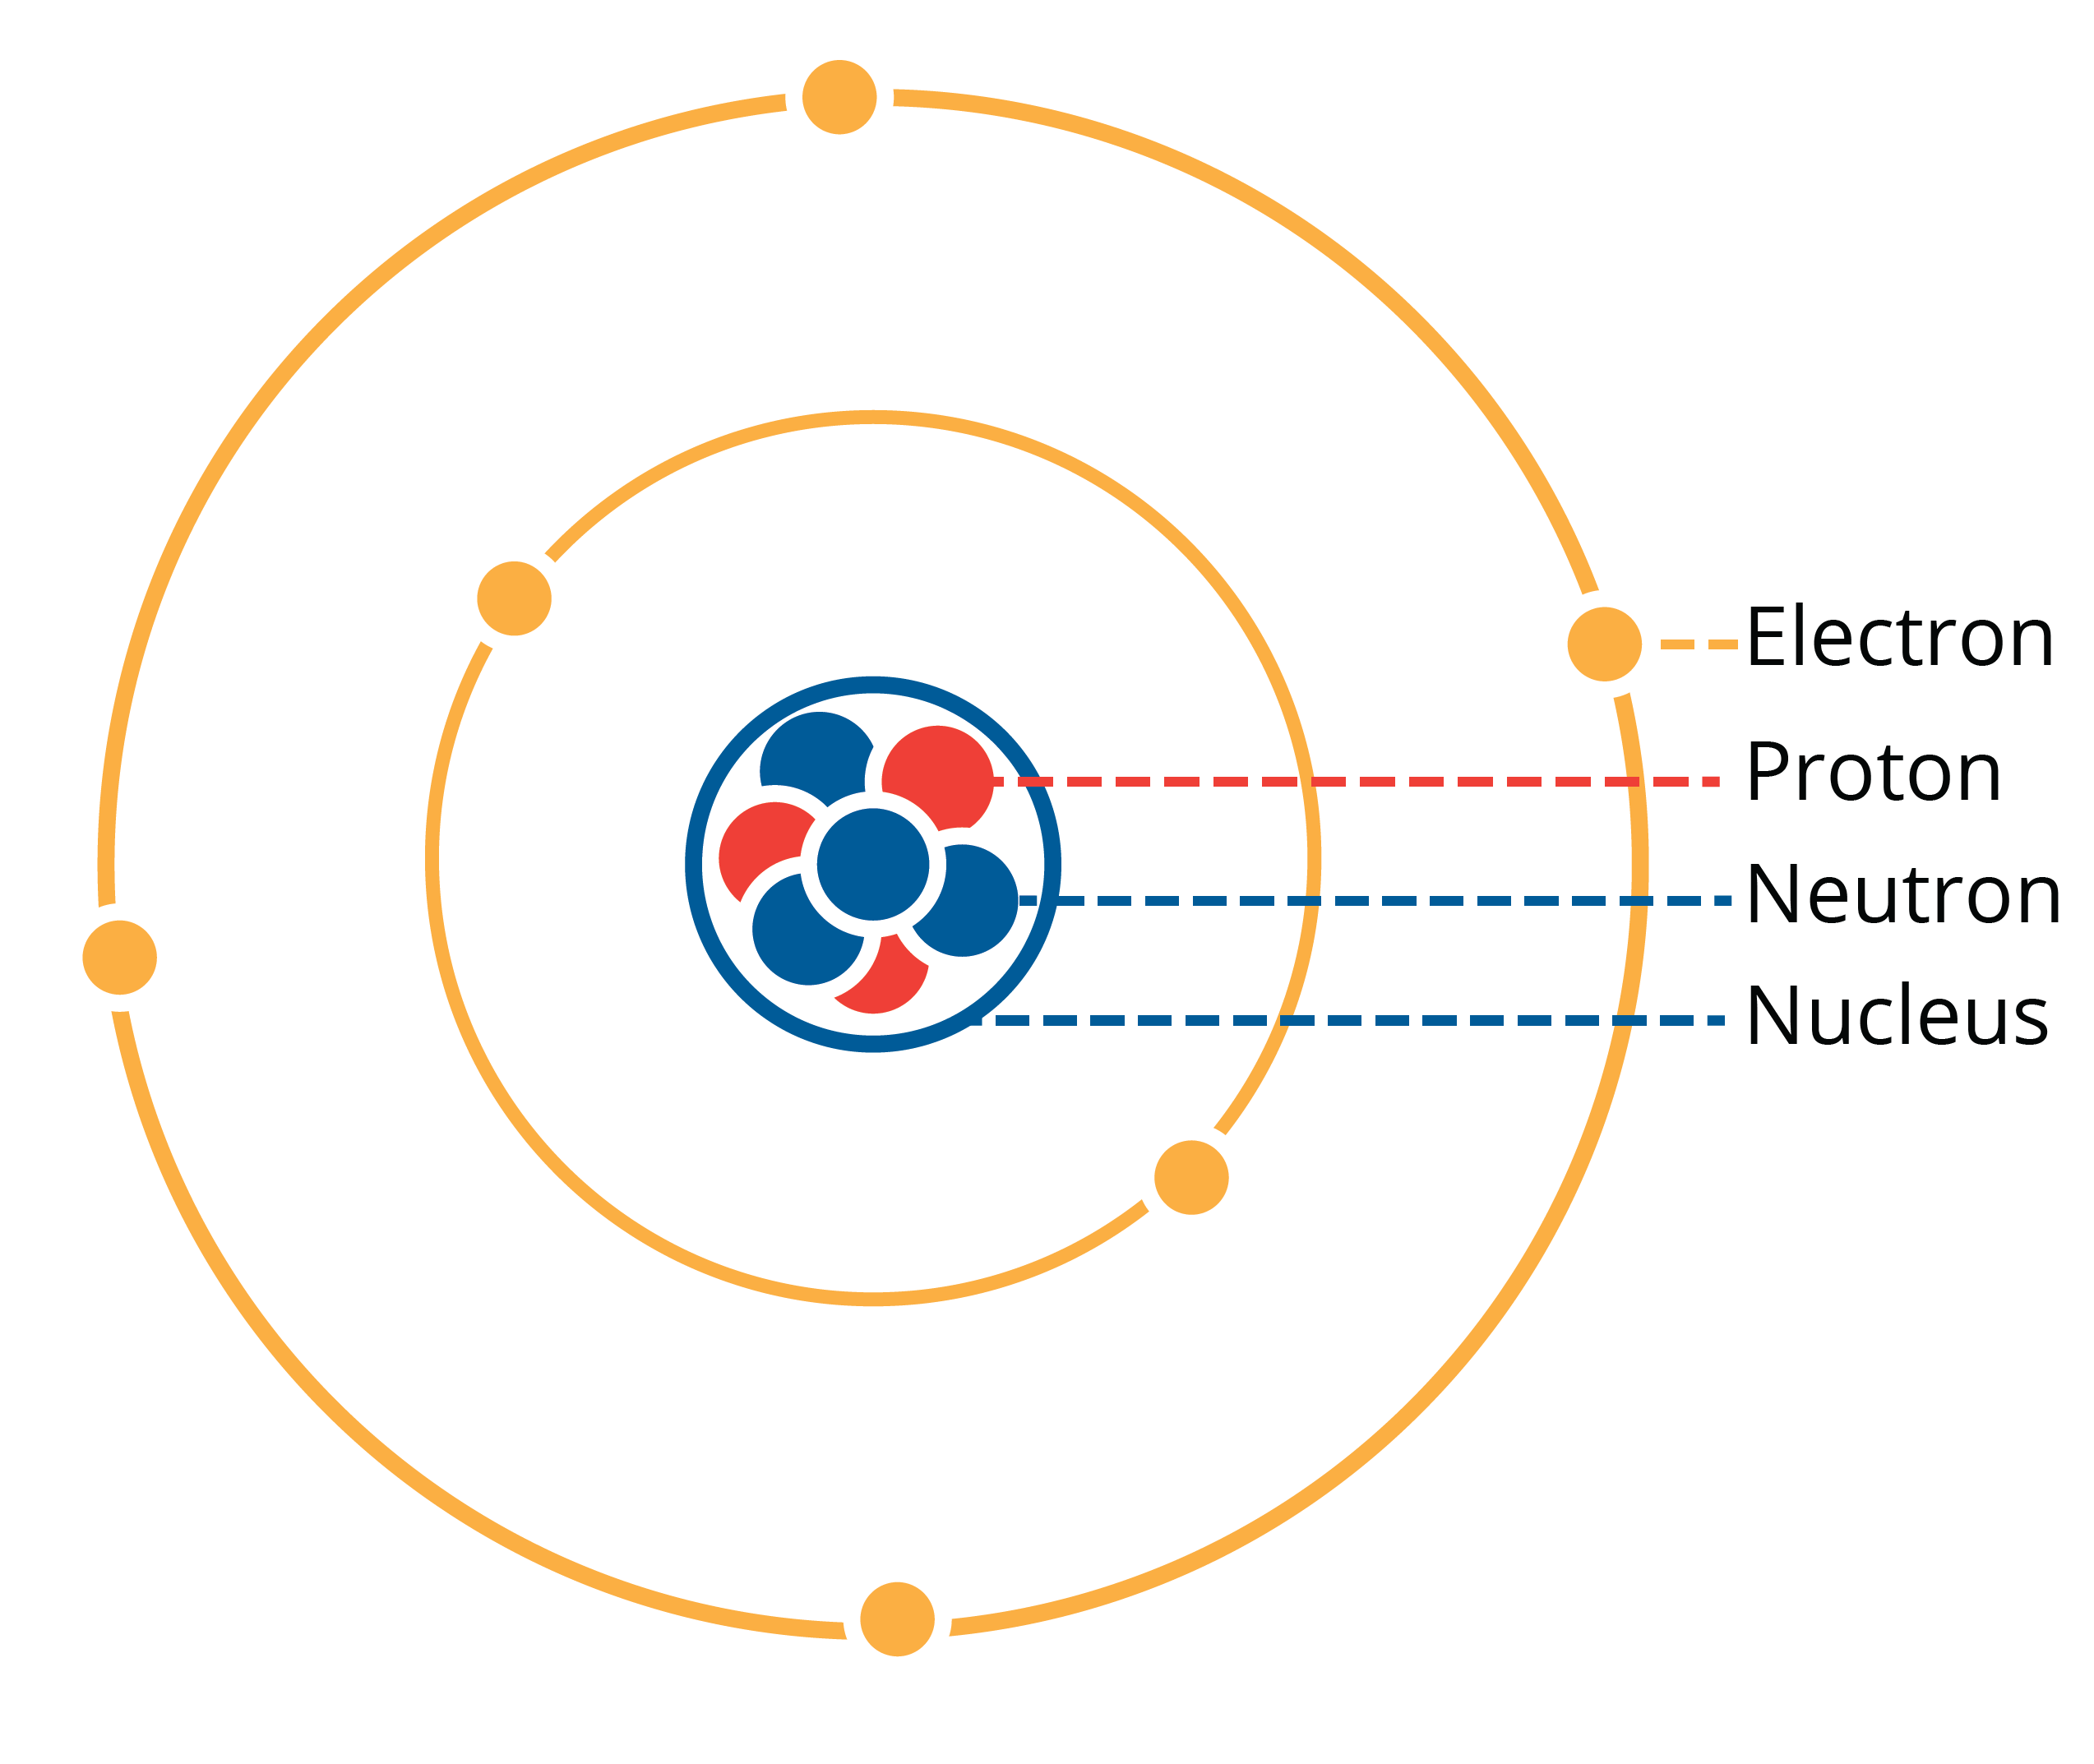
\includegraphics[width=2.5in]{atom1.png}
\caption{}
\label{fig:atom1}
\end{wrapfigure}

What is this ordinary matter made of? All things (including the air around you) 
are made of atoms. Atoms are incredibly tiny --- there are more atoms in a drop 
of water than there are drops of water in all the oceans.
% ADD: If you want a better visual of the scale: https://htwins.net/scale2/, start at around 10^-8

Every atom has a nucleus that contains protons and neutrons. Orbiting around the
nucleus is a cloud of electrons. However, the mass of the atom comes mainly from 
the protons and neutrons, since they are about 2000 times as massive as an 
electron! These three particles, protons, neutrons, and electrons, are called
\textit{subatomic particles}. (See figure \ref{fig:atom1}.) \index{protons} 
\index{neutrons} \index{electrons} \index{subatomic particle}

\section{Atoms and Their Models}
Over the history of science, there have been many ideas about the structure of
atoms. This history is a good example of how science develops: unexpected
results drive scientists to update their models, moving us closer and closer to
a true model of the atom.

During his investigations into the behavior of gases, John Dalton noted that 
different elements combine in strict ratios. For example, he noted that nitrogen 
and oxygen combine in a 1:1 and 1:2 fashion, but no ratio in between.

\begin{wrapfigure}{l}{3in}
\noindent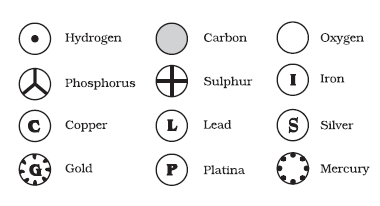
\includegraphics[width=2.5in, trim={0 0.5cm 0 0.5cm}, clip=true]{daltons_model.png}
\caption{Dalton modeled atoms as indivisible and unique.}
\end{wrapfigure}

This first model of the atom is rudimentary; each element is a unique atom,
and those atoms cannot be subdivided. The atom is modeled as one large, solid,
uniform, and neutral object. British physicist J.J. Thomson discovered that
atoms could be split into a light, negatively charged particle and a heavier,
positively charged particle (we now know this is the nucleus, the dense
grouping of protons and neutrons in the center of an atom).

Suddenly, the atom went from neutral and indivisible to made of different types
of charged particles. Further experiments by Ernest Rutherford showed the atom
to be mainly empty space, further updating scientists' model of the atom.
Subsequently, Bohr explained the phenomena of spectral lines (we will discuss
this further in Sequence 2) by modeling electrons as being restricted to
orbiting specific distances from the nucleus.

\begin{wrapfigure}{r}{3in}
\noindent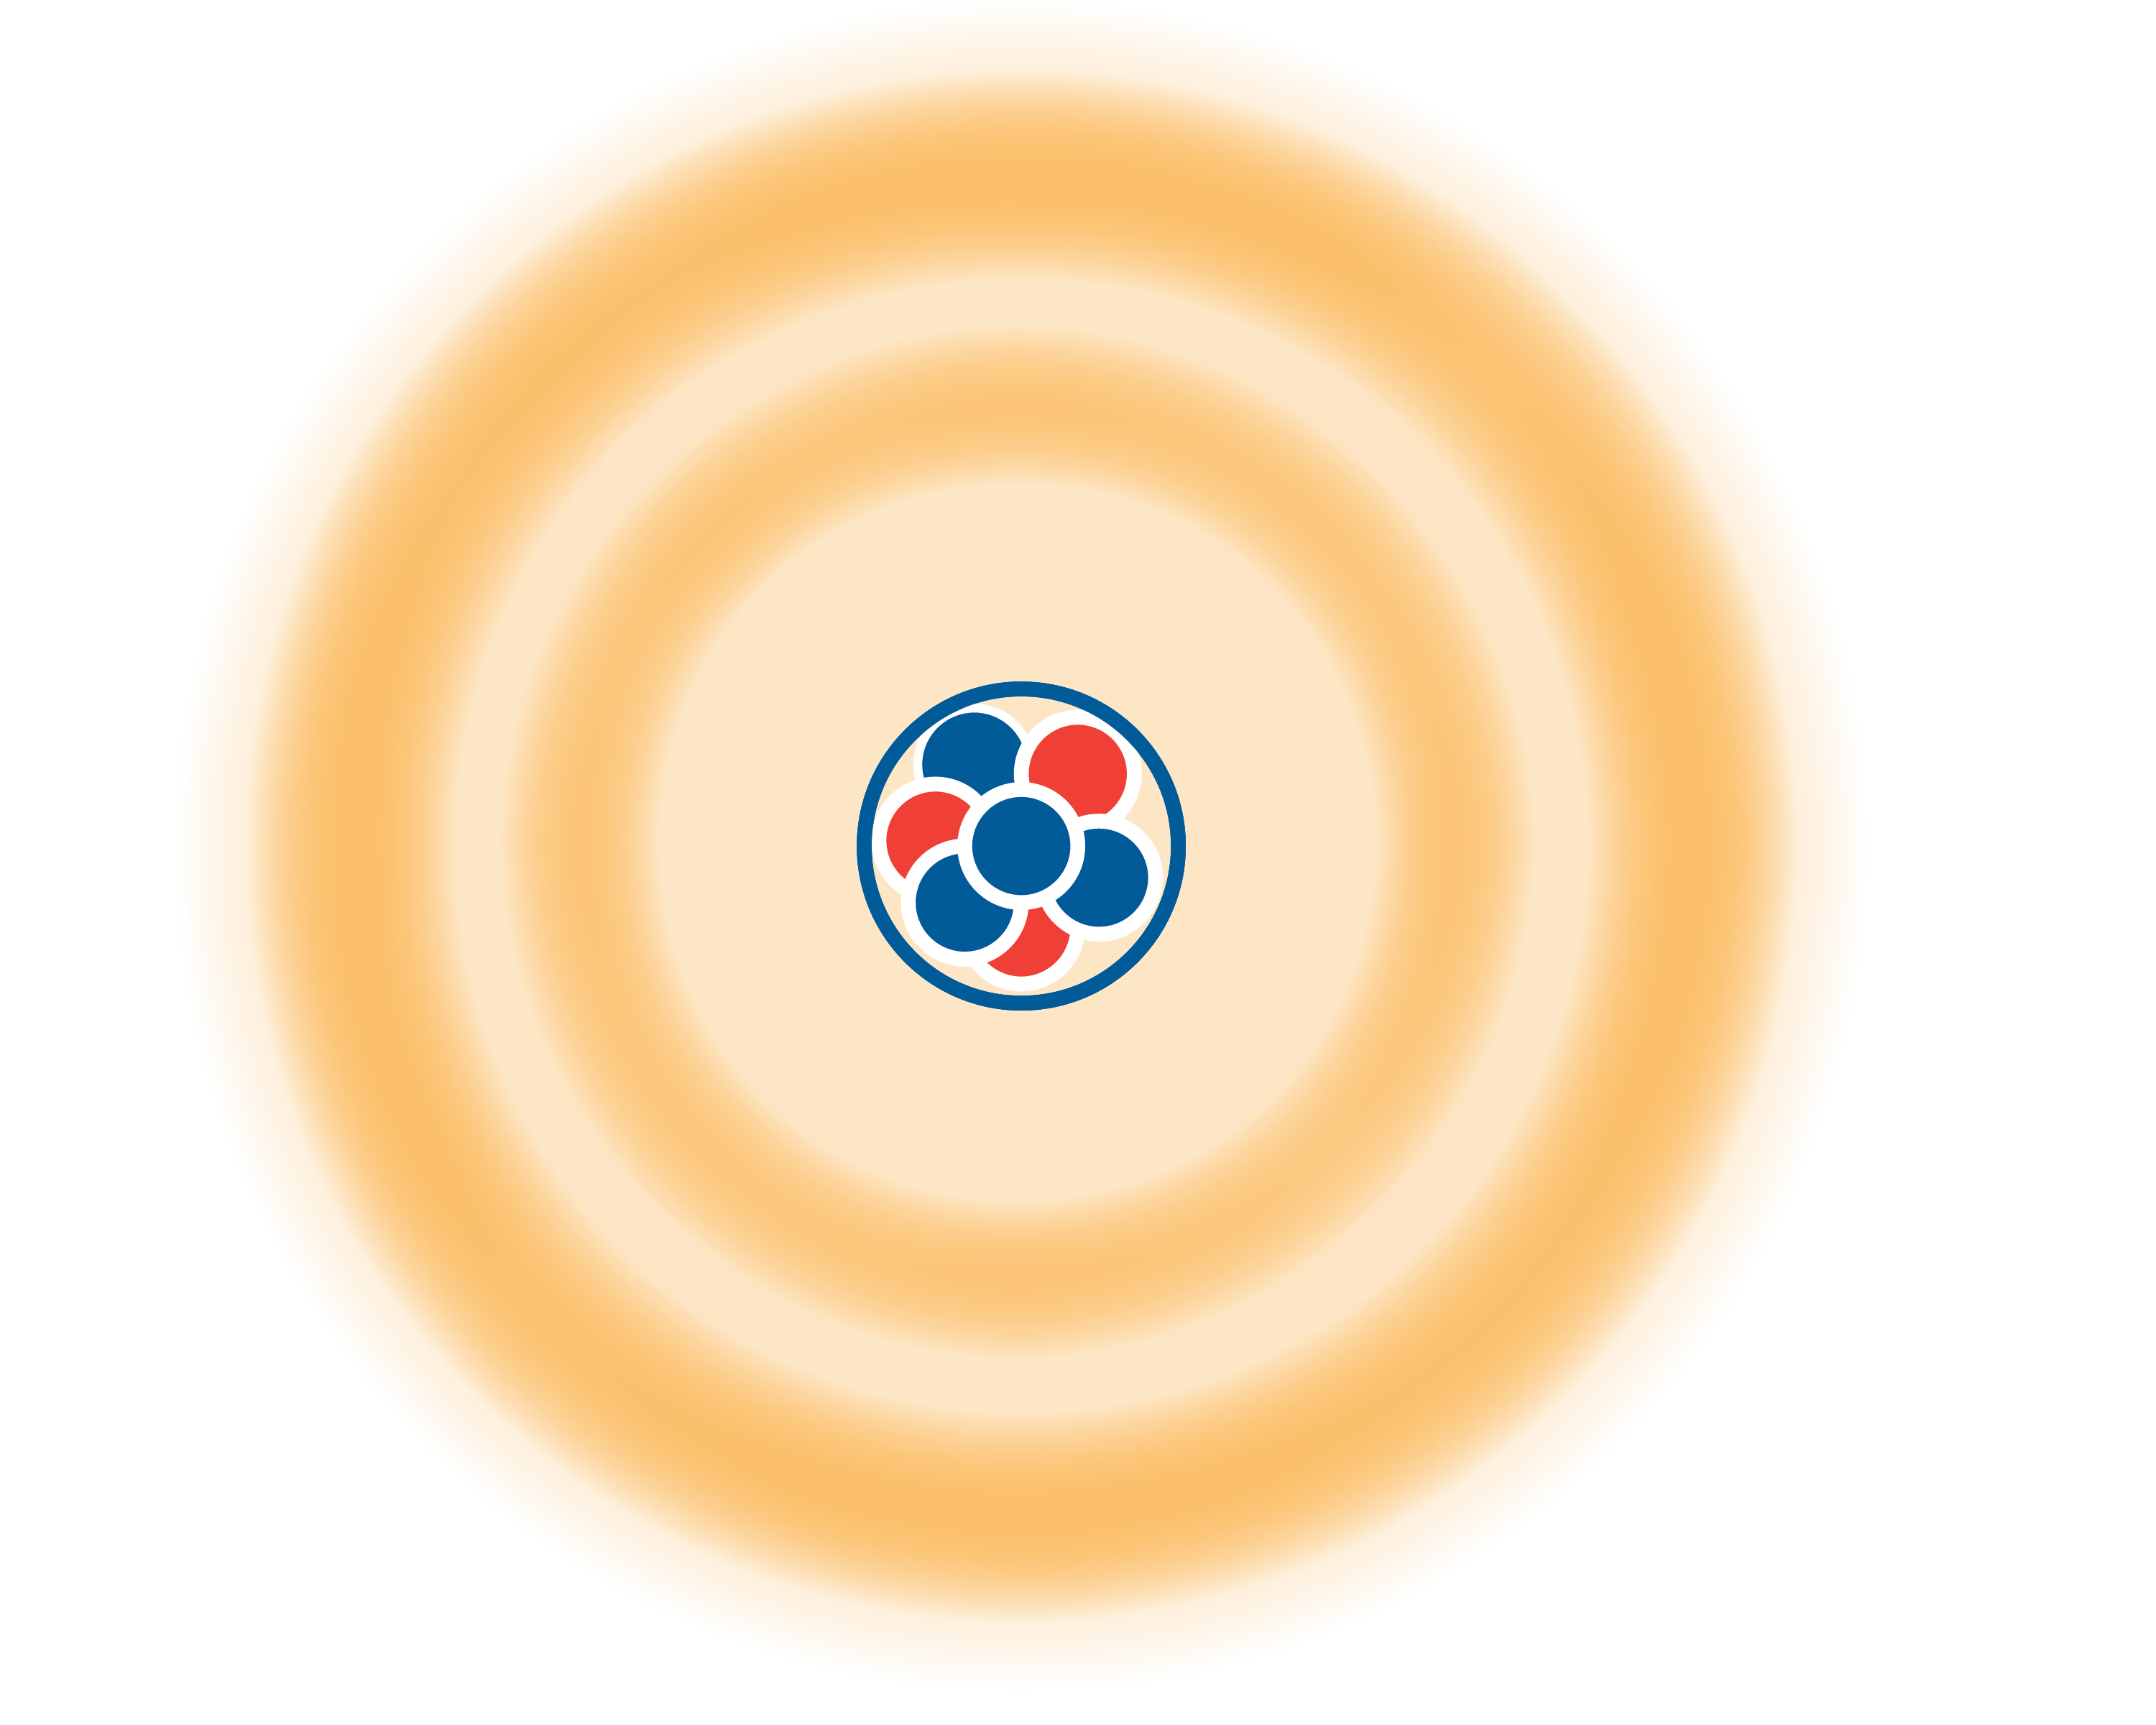
\includegraphics[width=3in]{atomCloud.png}
\caption{}
\label{fig:atomCloud}
\end{wrapfigure}

This is likely the model you are most familiar with seeing, and it is the one we
will use most often in this text. The first figure shown in this chapter is a Bohr
model: it shows the protons and neutrons in the nucleus, and models the electrons 
as moving in discrete orbits around the nucleus. 

However, the Bohr model is slightly inaccurate. While it is a convenient model for
thinking about atoms, in reality, electrons don't neatly orbit the nucleus.
Scientists don't know exactly where an electron will be in relation to the
nucleus, but they do know where it is most likely to be. They use a cloud that is
thicker in the center but fades out at the edges to represent an electron's
position (see figure \ref{fig:atomCloud}).

\begin{wrapfigure}{r}{3in}
\noindent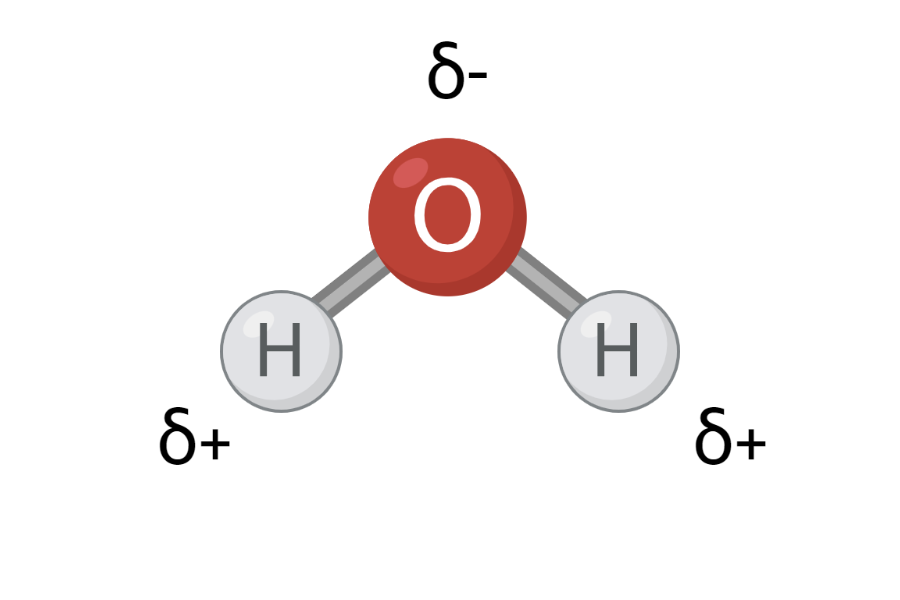
\includegraphics[width=3in]{water_polar.png}
\caption{}
\label{fig:water_polar}
\end{wrapfigure}

While the cloud model is more accurate, we will use the Bohr model as it
allows the viewer to easily and quickly assess the number and arrangement of
electrons.

\subsection{Classifying Atoms}

We classify atoms by the numbers of protons they have. An atom with one proton
is a hydrogen atom, an atom with two protons is a helium atom, and so forth
(refer to periodic table on pg..). We say that hydrogen and helium are \textit{
elements} because the classification of elements is based on the proton number.
And we give each element an atomic symbol. Hydrogen gets $H$, helium gets $He$,
oxygen gets $O$, carbon gets $C$\index{elements}, and so on.

\subsection{When Atoms Combine}
When atoms of different elements combine, they make \textit{compounds}. Compounds
are substances made up of more than one element. Compounds can be 
\textit{molecules} or \textit{crystal lattices}. In the next section you'll learn
\textit{why} these different structures form. 

There are many kinds of compounds. You know a few:
\begin{itemize}
\item Table salt is crystals made of $Na^{+}$ and $Cl^{-}$ ions: a sodium atom 
that as lost an electron and a chlorine atom that gained an electron
\item Baking soda, or sodium bicarbonate, is $NaHCO_3$.
\item $O_2$ is the oxygen molecules that you breathe out of the air (air, a
blend of gases, is mostly $N_2$.).
\item Common quartz is $SiO_2$: silicon dioxide
\end{itemize}

The subscripts indicate what ratio of the elements are present in the compound. 
Each number indicates the ratio for the preceding element. A drop of water, 
$H_2O$, has twice as many hydrogen atoms as oxygen atoms. 

\textbf{Example}: What is the ratio of elements present in Epsom salt?

\textbf{Solution}: Epsom salt, chemical name magnesium sulfate, has the chemical formula $MgSO_4$. Therefore, the ratio of Mg:S:O is 1:1:4. 

%fixme molecule vs formula unit, ordering of bonds versus formulas

\begin{Exercise}[title = {Numbers of Atoms in Molecules}, label = num_atom]
Give the elemental ratio for each compound. 
\begin{enumerate}
\item methane, $CH_4$
\item copper (II) sulfate, $CuSO_4$
\item glucose, $C_6H_{12}O_6$
\end{enumerate}
\end{Exercise}

\begin{Answer}[ref = num_atom]
\begin{enumerate}
\item C:H = 1:4
\item Cu:S:O = 1:1:4
\item C:H:O = 6:12:6 = 1:2:1
\end{enumerate}
\end{Answer}

\section{Types of Matter}
One way to classify matter is by the types of chemical bonds that hold a 
material's atoms together. The nature of these bonds, in turn, affects the 
properties of the material. For now, all you need to know is there are three types
of chemical bonds: metallic, covalent, and ionic. Materials held together with the
same type of bonds tend to have similar properties. For example, copper, bronze, 
iron, and steel (all containing metallic bonds) are all shiny, ductile, malleable,
and good conductors of heat and electricity. On the other hand, Epsom salt and 
table salt for large crystals, have very high melting points, and are poor 
conductors of electricity in their pure form. These two substances (Epsom and 
table salt) both contain ionic bonds. 

\subsection{Ionic Compounds}
Ionic bonds are the electrical attraction between opposite-charged ions. When a 
neutral atom gains or loses an electron it becomes an \textit{ion} (a charged 
atom), and oppositely-charged ions are attracted to each other. Which atom gets 
the electron and which loses it is based on their relative 
\textit{electronegativities}.\index{electronegativity} Electronegativity is simply
a measure of how strongly an atom can attract electrons to itself. In general, 
elements on the right side of the periodic table are more electronegative than 
elements on the left side. There are also polyatomic ions: groups of atoms held 
together with covalent bonds that have an overall charge (figure ... shows a Bohr 
model of a phosphate polyatomic ion, as an example). For now, we'll focus just on 
ionic bonds between monoatomic ions, like in table salt. You'll learn more about 
polyatomic ions and the compounds they form in Sequence 2. 

\begin{wrapfigure}{l}{3in}
\noindent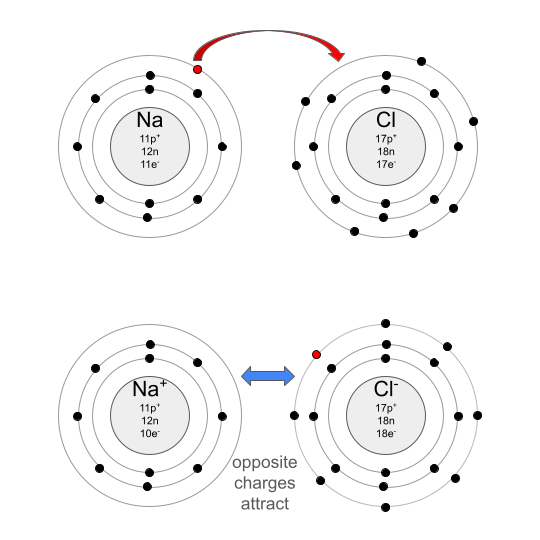
\includegraphics[width=3in]{NaCl_xfer.png}
\caption{}
\label{fig:NaCl_xfer}
\end{wrapfigure}

Let's examine how a simple ionic compound is formed: sodium chloride, also known 
as table salt, is made up of sodium and chlorine atoms (see figure 
\ref{fig:NaCl_xfer}). When sodium and chlorine come in contact with each other, 
electrons move from the sodium to the chlorine, making a sodium \textit{cation} 
(positively-charged ion) and a chloride \textit{anion} (negatively-charged ion). 
Yes --- chlor\textit{ide} is correct! When naming an anion, the ending of the 
element name changes to \textit{-ide}. Once the sodium cation and chloride anion 
are formed, their opposite charges attract them to each other, like north and 
south magnet poles. 

\begin{wrapfigure}{l}{3in}
\noindent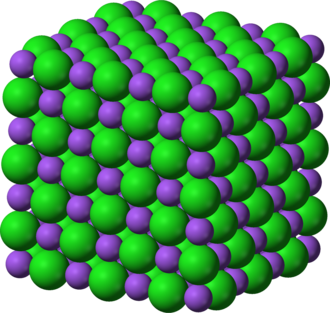
\includegraphics[width=2in]{NaCl_lattice.png}
\caption{}
\label{fig:NaCl_lattice}
\end{wrapfigure}

When there are many, many sodium and chloride ions around, they spontaneously 
arrange themselves in a pattern, giving ionic compounds their characteristic 
crystal structure (see figure \ref{fig:NaCl_lattice}). Because the electrons are 
tightly held be each ion, ionic substances don't conduct electricity well as 
solids. The atomic crystal lattice also determines the shape of the macroscopic 
crystals. Salt crystals are generally cubic, while other crystals (like quartz) 
form hexagonal prisms. You'll learn how to predict the atomic and macroscopic 
crystal structure of different compounds in Sequence 2. 

\subsection{Covalent Compounds}
Water is an example of a covalent compound: it is made of two hydrogen atoms 
covalently bonded one oxygen atom (see figure \ref{fig:water_polar}). The result 
is a water molecule\index{molecules}. The different atoms cluster together 
because they share electrons in their clouds. This is the nature of a 
\textit{covalent bond}\index{covalent bond}: it is formed when atoms share electrons.
Sometimes, electrons are shared evenly, but in water, they are shared unevenly. 
Due to the difference in electronegativity between hydrogen and oxygen, the 
shared electrons are more attracted to the oxygen atom than the hydrogen atoms, 
so they spend more time on the oxygen atom. As a result, the oxygen side of a 
water molecule has a slight negative charge, while the hydrogen atoms have a 
slight positive charge. The slight charges are represented with a lower case 
Greek letter delta, $\delta$. When electrons are shared unevenly, we call this a
\textit{polar} covalent bond, because there are positive and negative poles at 
either end of the bond. \index{polar bond} \index{non-polar bond}

When covalent bonds form between two elements of similar electronegativities, 
the electrons are shared evenly. We call this a \textit{non-polar} covalent bond. 
Oil is an example of a non-polar covalent substance. Different oils have different
combinations, but all oils are made mainly of carbon and hydrogen, which have similar
electronegativities. For both polar and non-polar covalent bonds, the electrons 
are still held tightly, even if they are shared. Those electrons don't move to 
another molecule: they move around within the molecule they are already a part 
of. Since electrons don't flow freely in covalent substances, they are also poor 
conductors of electricity. But, they generally have lower melting and boiling 
points than ionic compounds. 

What happens when you try to mix oil and water? They don't mix well! This is due 
to the difference between their bond types. Polar substances, like water, mix best
with other polar substances, while non-polar substances, like oils, mix best with 
non-polar substances. You'll learn more about why this is in Sequence 2.

\subsection{Metallic Compounds}
You may already know that metals (both pure and alloyed) are excellent conductors of electricity and heat. This is a consequence of their metallic bonds. 
%fixme complete section, pure vs alloys, free flowing electrons



\section{Energy and Work}

Energy is defined as the ability to do work, but what does this mean? First, we 
need to understand what \textit{work} is. When you lift an object into the air, 
you are doing work on that object. When water turns a turbine in a hydroelectric 
plant, the water is doing work on the turbine. And when you hit the brakes on your
car, the brake pads are doing work on the tires (albeit, negative work). 
\textit{Energy} is being transferred between these pairs of objects when work is 
done. 

Some everyday examples of energy include:
\begin{enumerate}
\item The Calories in your food
\item The light from the Sun
\item Heat in the Earth's mantle
\item The motion of a spinning wheel
\end{enumerate}

Some types of energy are easy to visualize, while others are not. Energy is what 
moves from one object to another when work is being done. When you lift 
something, the energy stored in your body (in the form of sugar and fat) is 
transferred to the object, accelerating it upwards. Your body continues to 
transfer energy as you lift the object against gravity. When you've lifted it as 
high as you can, most of the energy your body lost (we call this "burning 
Calories" colloquially) is stored as \textit{potential energy}, due to the 
object's height. 

Another example is a simple circuit connecting a battery and a light bulb. The 
battery has stored potential energy. When the circuit is complete, the potential 
energy in the battery is transferred to electrons in the light bulb, causing them 
to move and gain kinetic energy. In the light bulb's filament (we are referencing 
old, non-LED light bulbs here!), the electrons encounter resistance, which slows 
them down. The energy the electrons lose in this process is being transformed into 
light and heat, lighting your room. 

%fixme edit/rehome material below



\section{Chemical Reactions}

\begin{wrapfigure}{l}{3in}
\noindent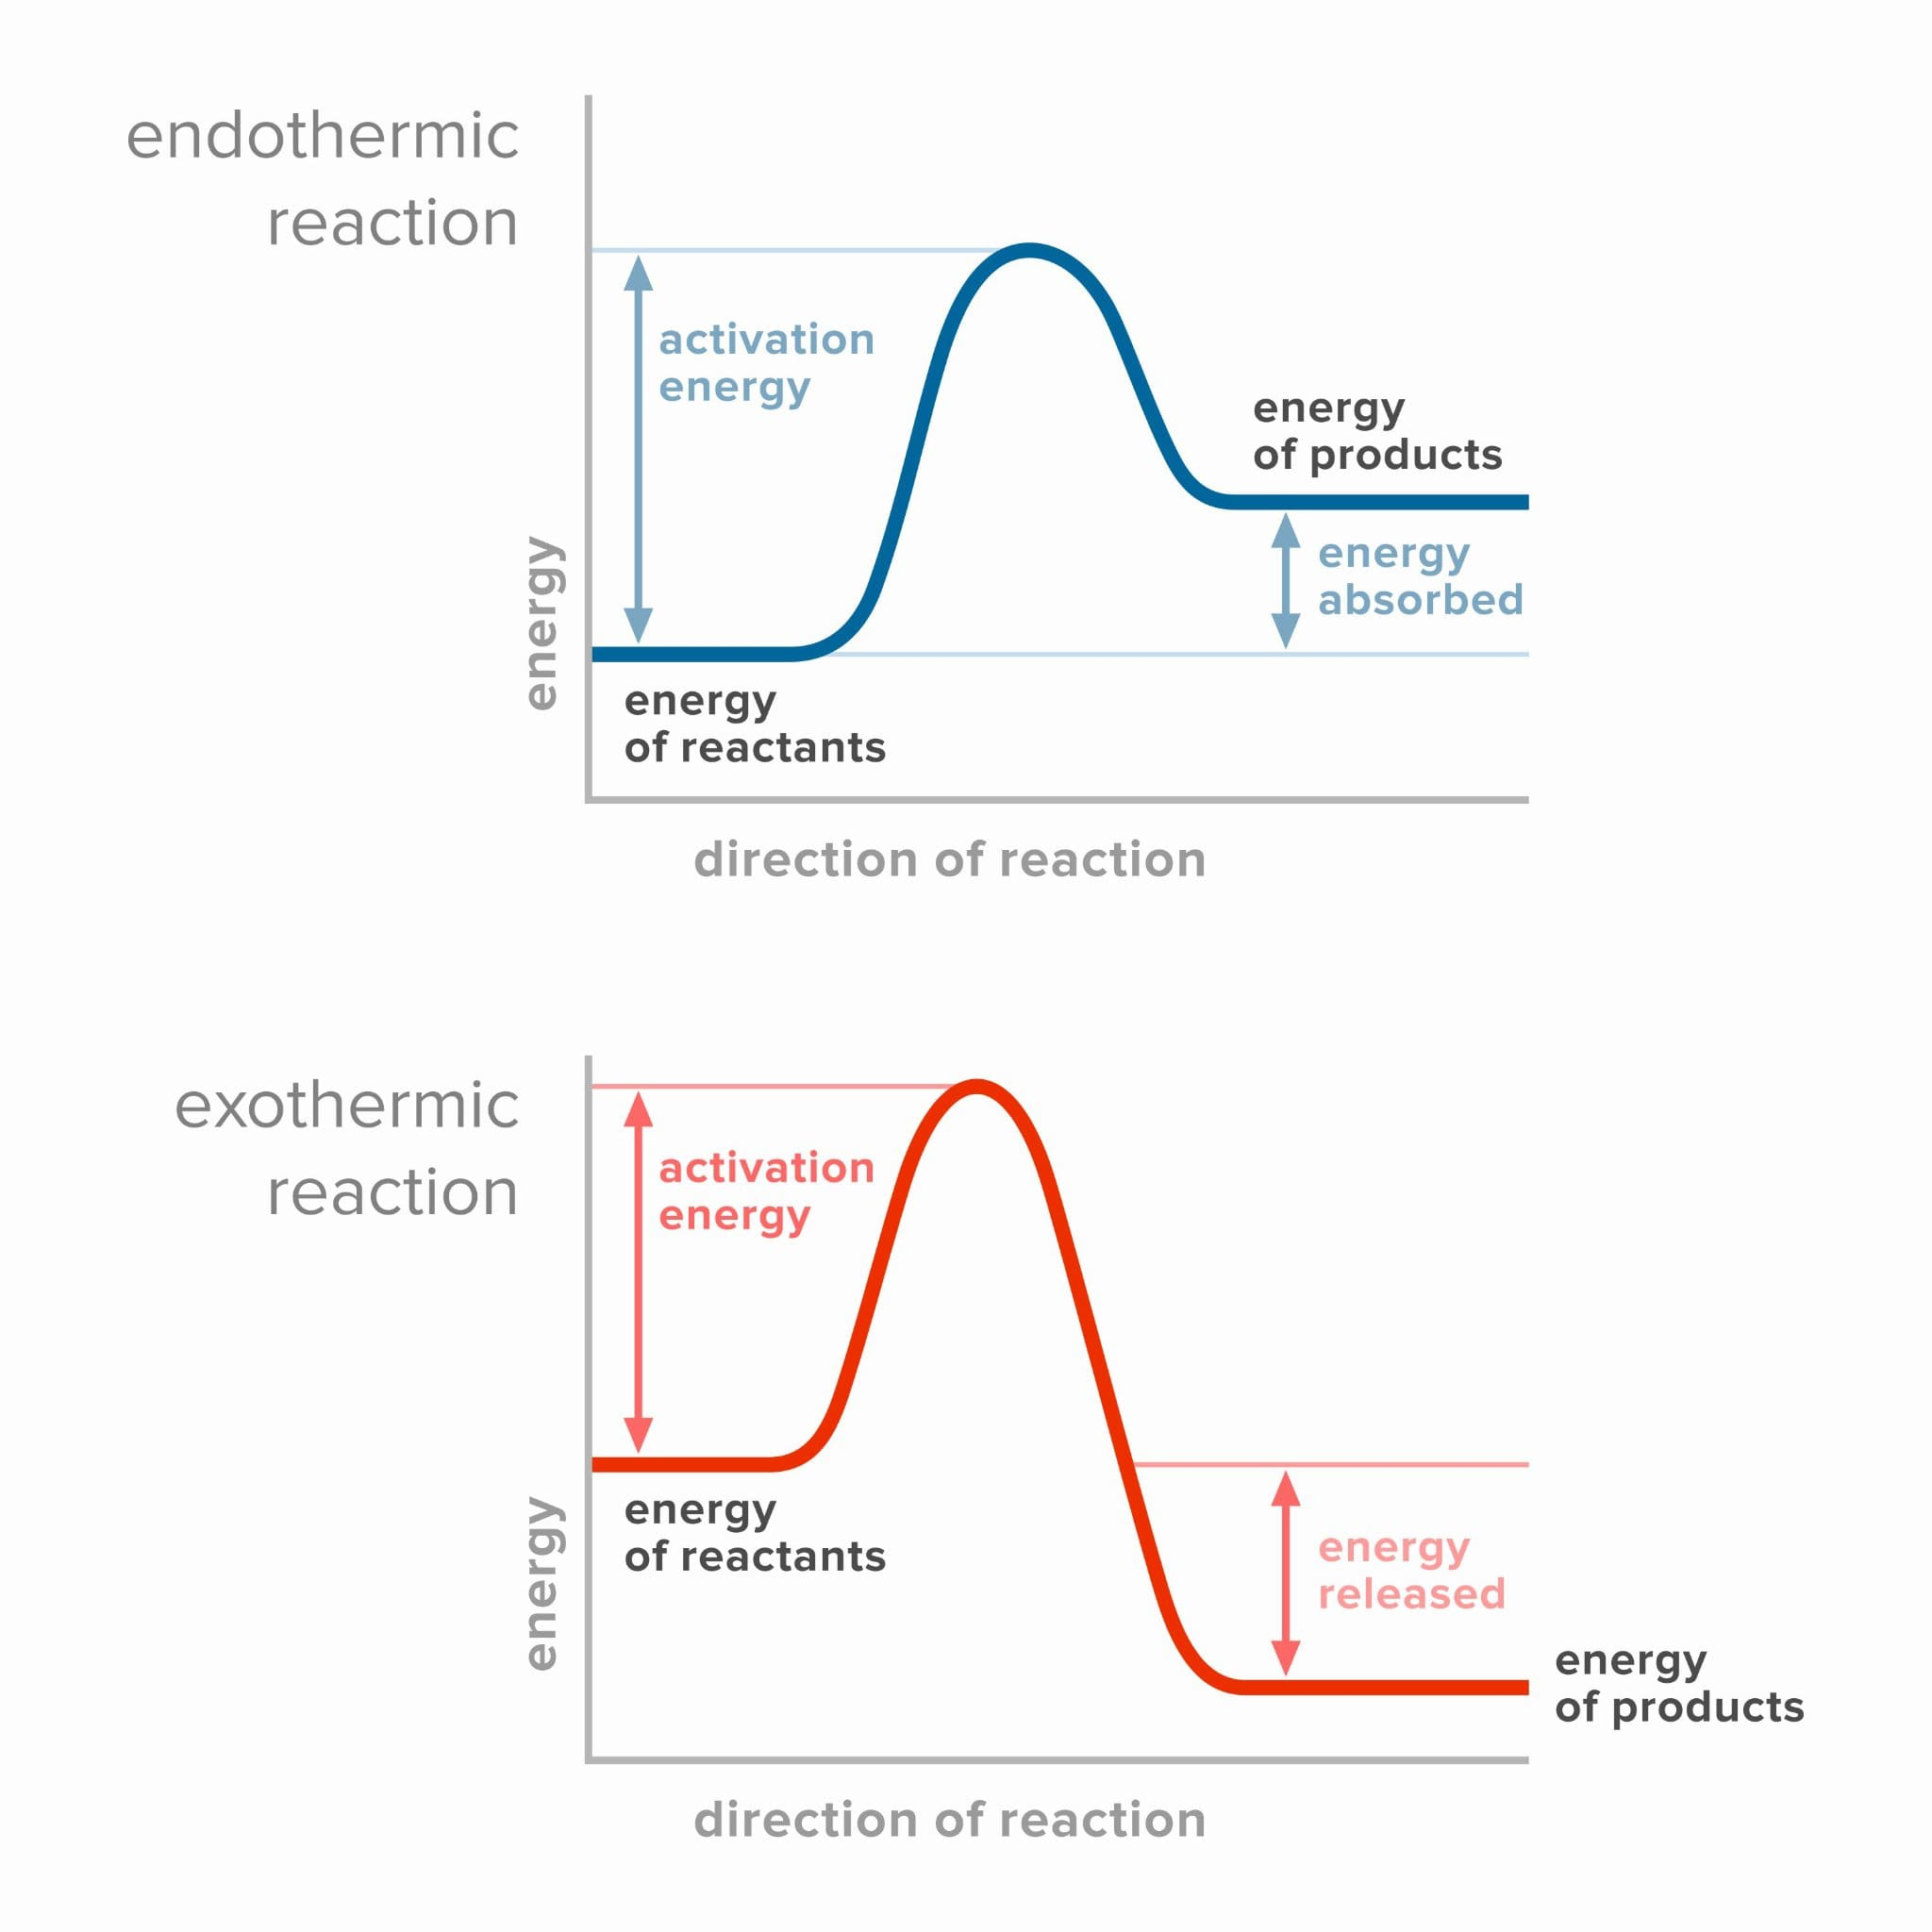
\includegraphics[width=3in]{exo_endo_diagrams.png}
\caption{}
\label{fig:exo_endo_diagrams}
\end{wrapfigure}

Sometimes two hydrogen atoms form a molecule ($H_2$). Sometimes two oxygen
atoms form a molecule ($O_2$). If you mix these together and light a match,
they will rearrange themselves into water molecules. This is called a \textit{
chemical reaction}. In any chemical reaction, the atoms are rearranged into new
molecules.\index{chemical reaction}

Some chemical reactions (like the burning of hydrogen gas described above) are
\textit{exothermic} --- that is, they give off energy. Burning hydrogen gas
happens quickly and gives off a lot of energy. If you have enough, it will make
quite an explosion! \index{exothermic}

Other chemical reactions are \textit{endothermic} --- they consume energy.
Photosynthesis, the process by which plants consume energy from the sun to make
sugar from $CO_2$ and $H_2O$ requires an endothermic chemical reaction.\index{endothermic}

Examine the diagrams in figure \ref{fig:exo_endo_diagrams}. The $x$-axis 
represents time - time passes as wemove from left to right across the diagram. 
At the far left, the energy of the reactants (the ingredients that go into the 
reaction) is shown. At the far right, the energy of the products (what is made in 
the chemical reaction) is shown. The red diagrams shows an exothermic reaction: 
the products (what is made) have less energy than the reactants (the "ingredients"
that start the reaction). Since energy is never created or destroyed, where did 
the energy go? It is released as heat. So, exothermic reactions release heat.

Now, look at the endothermic reaction diagram (the blue one). Based on the
relative energies of the reactants and products, do you expect and endothermic
reaction to release or absorb heat? Absorb! Since the products have more
energy, they must have absorbed energy, in the form of heat, from the surroundings.

What does this look and feel like in real life? If an exothermic reaction were
happening in a glass beaker, you would feel warmth if you held the beaker. The
heat is leaving the beaker and entering your hand, which feels warm. What
about an endothermic reaction? Many students think that since an endothermic
reaction absorbs heat, it must be getting hot. This is incorrect:
\textit{exothermic} reactions feel hot. If an endothermic reaction were
happening in a beaker and you touched the beaker, it would feel \textbf{cold}.
Why? Well, if the reaction is absorbing heat, then heat must be leaving it
surroundings (your hand) and entering the reaction (this heat energy is turned
into chemical energy that is stored in the new chemical bonds that are
forming). So your hand feels cold. %fixme: models showing flow of heat in/out of system for chemical reactions.

\section{Mass and Acceleration}

Each atom has a mass, which means everything made up of those atoms has mass as 
well (and that's pretty much everything!). We measure mass in grams. A paper clip 
is about 1 gram of steel. An adult human can have a mass of 70,000 grams, so for 
larger things, we often talk about kilograms, which is 1000 grams.

The first interesting thing about mass is that objects with more mass
require more force to accelerate. For example, pushing a bicycle so
that it accelerates from a standstill to jogging speed in 2 seconds
requires much less force than pushing a train so that it accelerates
at the same rate.


\begin{mdframed}[style=important, frametitle={Newton's Second Law of Motion}]

The force necessary to accelerate an object of mass $m$ at an acceleration of
$a$ is given by:
$$F = m a$$

This means the force is equal to the mass times the acceleration.

\end{mdframed}

What are the units here? We already know that mass is measured in
kilograms. We can measure velocity in meters per second, but that is
different from acceleration. Acceleration is the rate of change in
velocity. So if we want to go from 0 to 5 meters per second (that's
jogging speed) in two seconds, that is a change in velocity of 2.5
meters per second every second. We would say this acceleration is $2.5
m/s^2$.

\subsection{Calculating Acceleration}
As suggested above, acceleration is a change in velocity. It is calculated by
dividing the change in velocity by the time it takes to make that change.

\begin{mdframed}[style = important, frametitle = {Calculating Acceleration}]
The acceleration of an object from an initial velocity, $v_i$, to a final
velocity, $v_f$, over a period of time, $t$, is given by:

$$a = \frac{v_f - v_i}{t}$$
\end{mdframed}

\textbf{Example}: Your car can go from zero to 60 mph in 3 seconds. What is the
acceleration in $m / s^2$?

\textbf{Solution}: First, let's convert from the imperial units of miles per
hour to the SI units of meters per second. You can do this using a search engine, 
but we will show how to do it by hand below. (You will learn more about this 
method in the Units chapter).

$$\frac{60 \text{ miles}}{1 \text{ hour}} \cdot \frac{1.61 \text{ km}}{1 
\text{ mile}} \cdot \frac{1000\text{ m}}{1\text{ km}} \cdot \frac{1\text{ hour}}{
3600\text{ seconds}} \approx \frac{26.82\text{ m}}{s}$$

Now we have the starting velocity (0 m/s), the ending velocity (26.82 m/s), and 
the time (3 s), and we can find the acceleration:
$$a = \frac{v_f - v_i}{t} = \frac{26.82\frac{m}{s} - 0\frac{m}{s}}{3s} \approx 
8.94 \frac{m}{s^2}$$

\subsection{Determining Force}
What about measuring force? Newton decided to name the unit after himself: The
force necessary to accelerate one kilogram at $1 m/s^2$ is known as \textit{a
newton}. It is often denoted by the symbol $N$.

$$1 N = 1 \frac{kg \cdot m}{s^2}$$

\textbf{Example}: If the car in the above example has a mass of 1500 kg, how much 
force does the engine use to accelerate the car?

\textbf{Solution}: We have already found the car's acceleration: 8.94 $m/s^2$. 
With the mass and acceleration, we can use Newton's Second Law to find the force 
needed to accelerate the car:
$$F = m \cdot a = 1500\text{ kg} \cdot 8.94 \frac{m}{s^2} = 13410\text{ N}$$

\begin{Exercise}[title={Acceleration}, label=acceleration_train]

While driving a bulldozer, you come across a train car (with no brakes
and no locomotive) sitting on a track in the middle of a city. The train car
has a label telling you that it has a mass of 2,400 kg. There is a time-bomb
welded to the interior of the train car, and the timer tells you that
you can safely push the train car for 120 seconds. To get the train
car to where it can explode safely, you need to accelerate it to 20 meters per
second. Fortunately, the track is level and the train car's wheels have
almost no rolling resistance.

With what force, in newtons, do you need to push the train for those 120 seconds?

\end{Exercise}
\begin{Answer}[ref=acceleration_train]
If you accelerate to 20 m/s in 120 s, the acceleration is:
$$a = \frac{v_f - v_i}{t} = \frac{20\text{ m/s} - 0\text{ m/s}}{120\text{ s}} = 
\frac{1}{6} \frac{m}{s^2}$$

To achieve this acceleration, you will need to apply a force of:
$$F = m \cdot a = 2400\text{ kg} \cdot \frac{1}{6} \frac{m}{s^2} = 400\text{ }N$$
\end{Answer}



%FIXME Global layout note: Let's discuss adding Title's and Captions to all graphics.\\

%For example:\\
%TITLE: Mass versus Weight\\
%CAPTION: Human Earth weight: 150lbs / Moon weight:??lbs\\
%Potato Earth weight: .25lbs / Moon weight: ??lbs \\

%FIXME:
%Allison thinks it would be funny if the person in the graphic were holding a potato and we also added the weight and mass of the potato to the caption. No worries if this type of edit isn't in the budget!

%FIXME: What are your thoughts about using the metric system consistently -- in which case we'll replace pounds here with kilos. Max notes: we should explicitly use kilos for mass and pounds or newtons for weight. Kilos are a scalar measure of the amount of matter and pounds are a vector force of gravity on a particular piece of matter. Many students struggle to differentiate between mass and weight at a theoretical level due to casual comparison between pounds and kilos.

\graphicspath{{../../Chapters/atomic_mass/en_US}}
\chapter{Atomic and Molecular Mass}

%fixme add hook

\section{Reading a Periodic Tile}

Let's look at the different information shown on a periodic tile:

\begin{center}
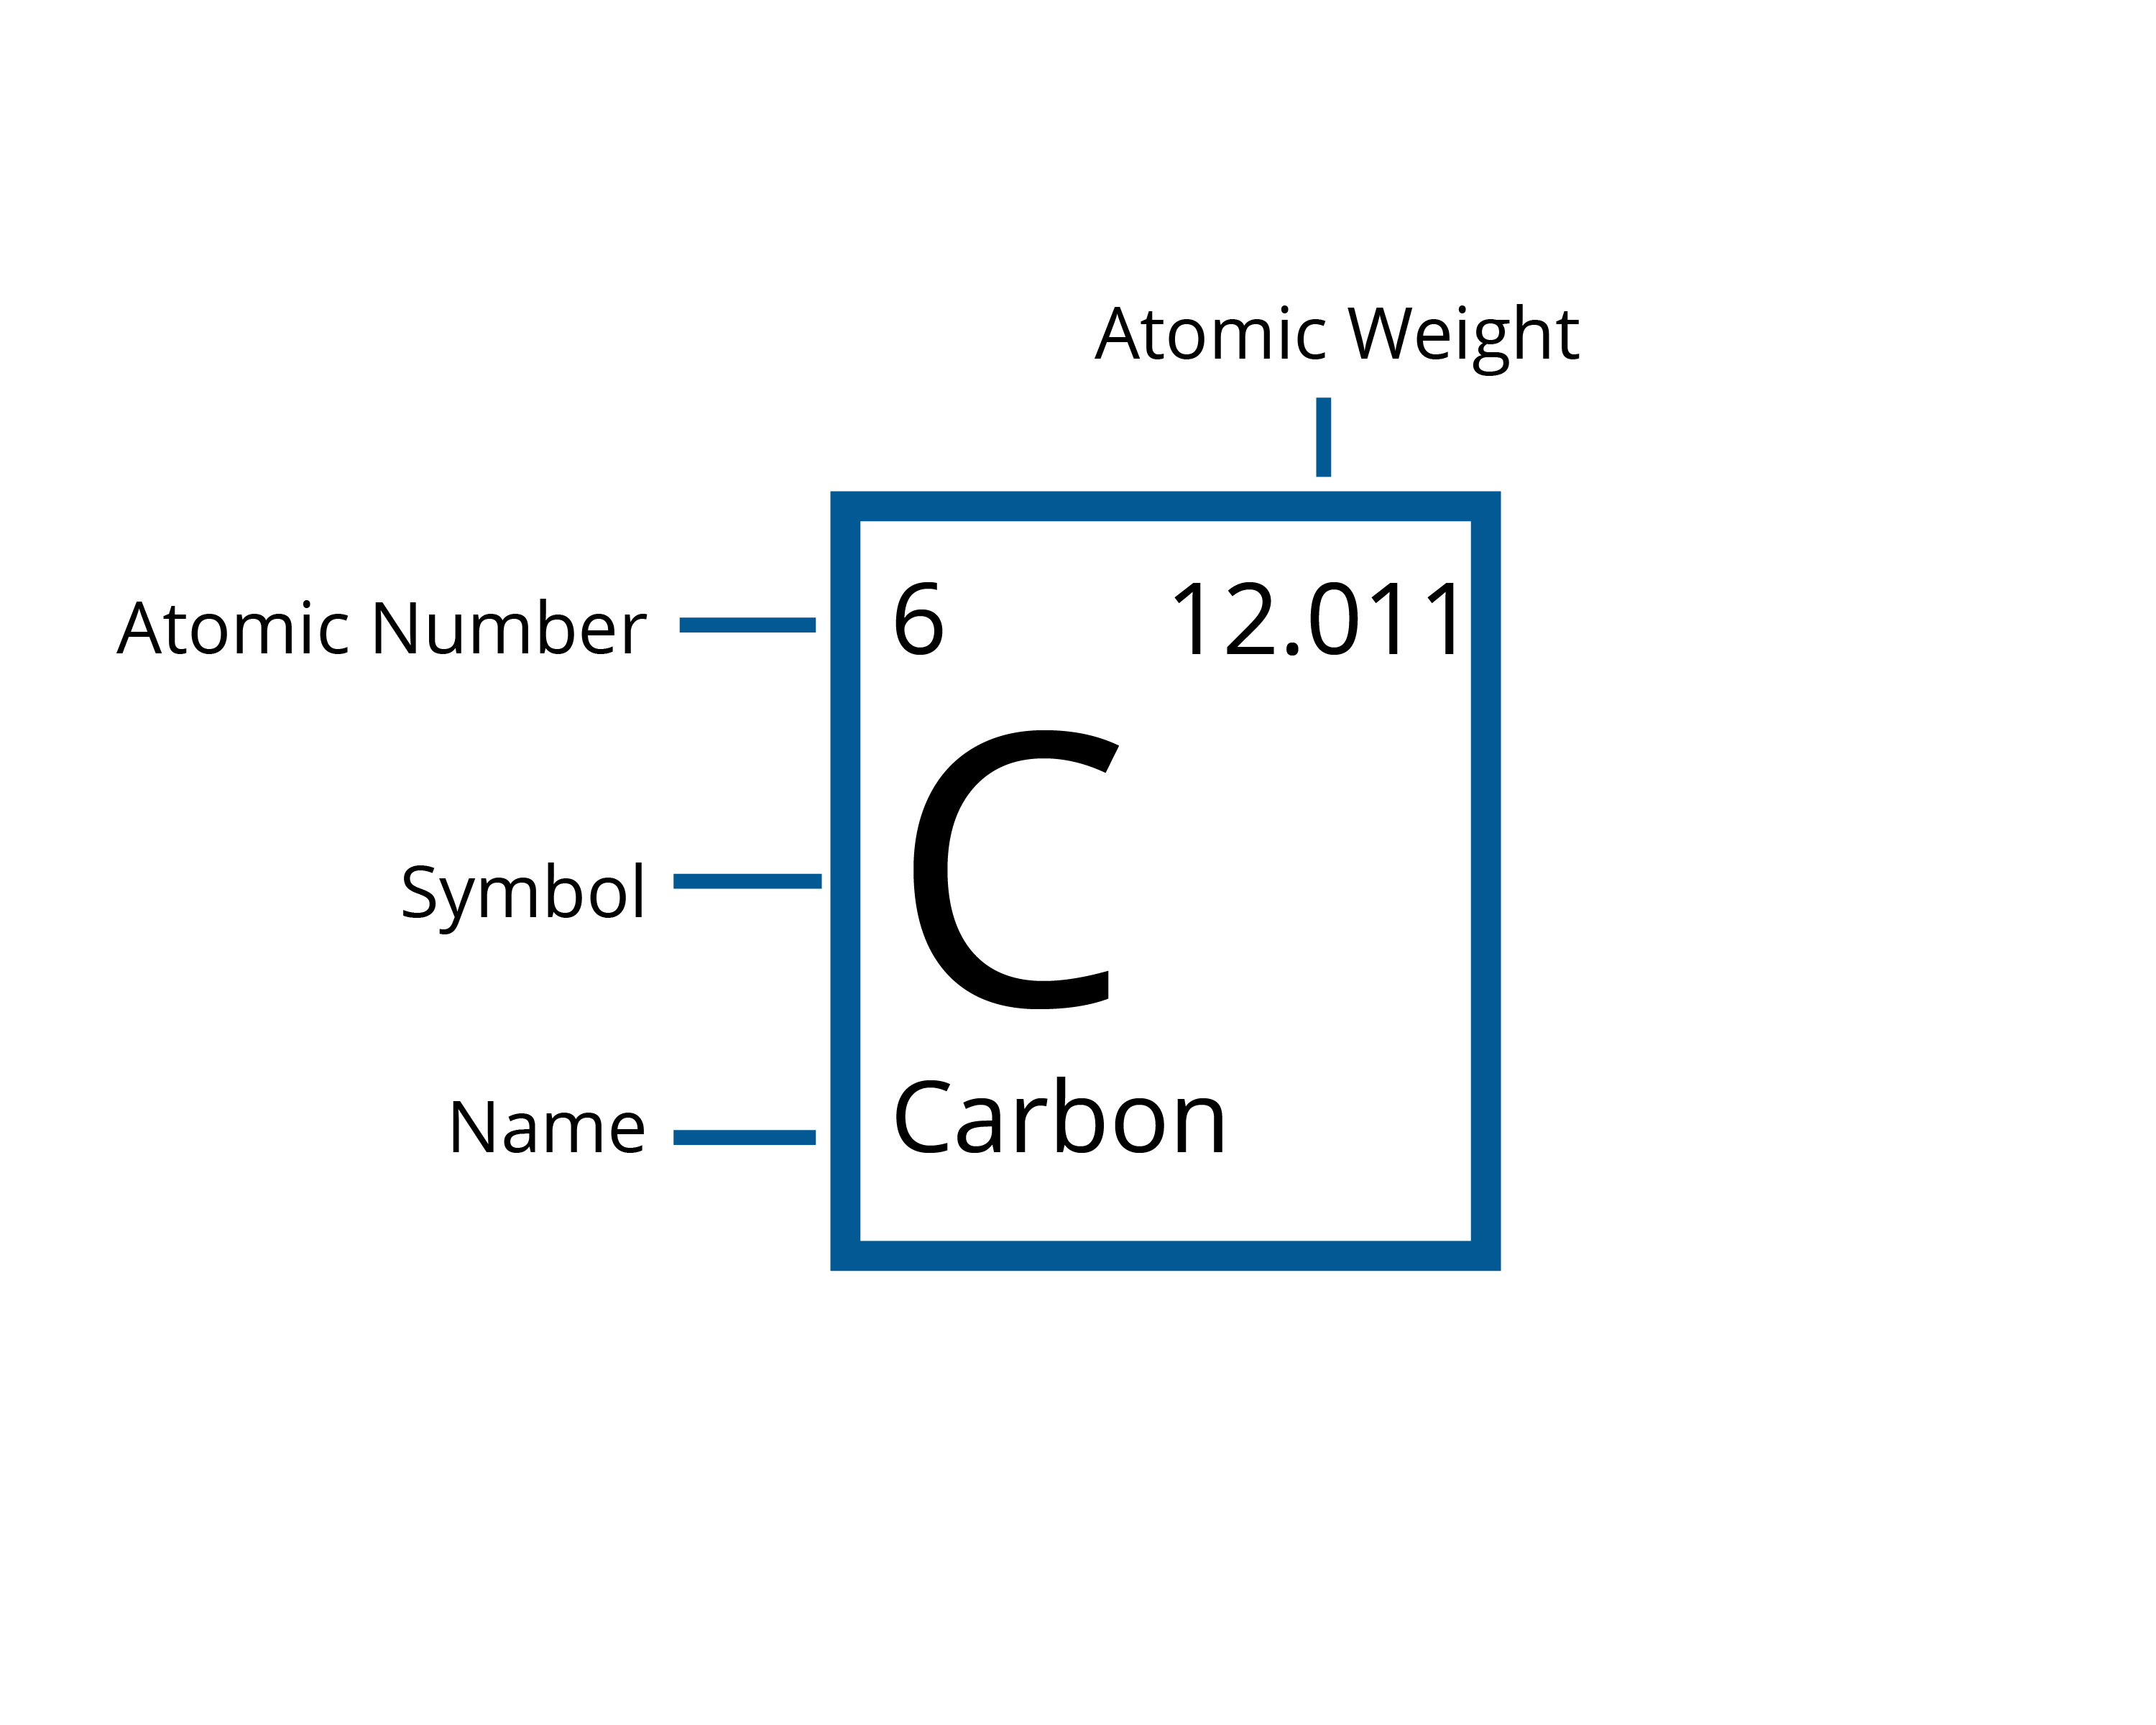
\includegraphics[width = 4in]{element.png}
%fixme change "weight" to "mass" or remake image
\end{center}

The four things we learn from a periodic tile are:
\begin{enumerate}
\item the symbol: as discussed in the previous chapter, each element has a 
unique symbol. Element symbols are used when showing the structure of a molecule
and modeling chemical reactions. 
\item the atomic number: this is also unique for each element. Take a look at the
periodic table a few pages forward. Every tile has a unique atomic number, and 
the tiles are laid out in a generally increasing atomic number (you'll learn why
the periodic table is arranged this way in Sequence 2). 
\item the atomic weight: this is the average mass of all the atoms of that element
in existence. Just like your overall grade in a class is the weighted average of
all the individual grades you earned, atomic weight is the weighted average of the
masses of all the individual atoms of that element. This is also sometimes referred to as atomic mass.
\item the name: not all periodic tables show the name of an element on its tile.
This is why it is useful to know the symbols of common elements. 
\end{enumerate}

Recall from the previous chapter that we classify atoms by the number of protons
they have. What this means is that if we want to know what element an atom is, we
have to look at the number of protons. Take a look at the three carbon atoms below
and note what is the same and what is different among them:

\begin{center}
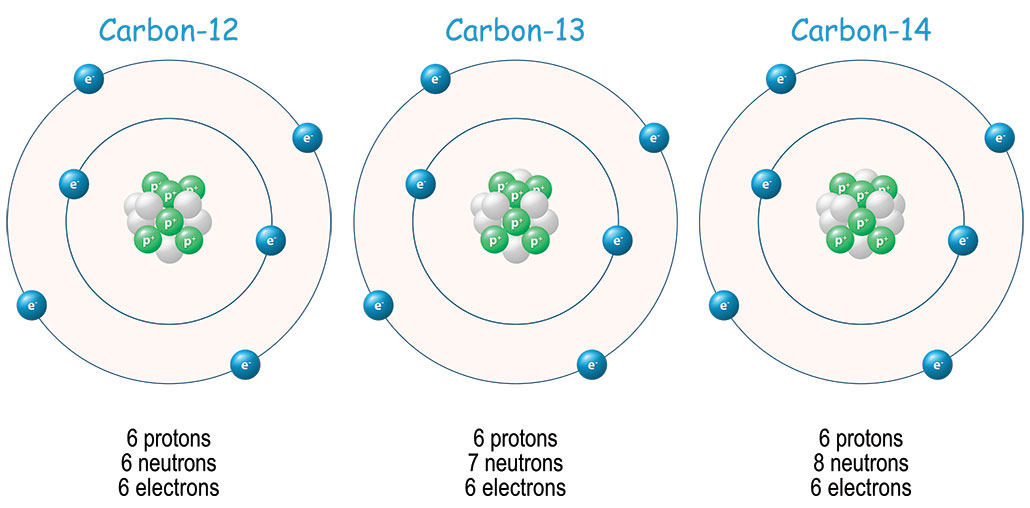
\includegraphics[scale=0.35]{carbon_iso.png}
\end{center}

These different versions of carbon all have 6 protons, which is also carbon's 
atomic number. This isn't a coincidence: the atomic number \textit{is} the number
of protons in every atom of an element. If I tell you an atom has 4 protons, you 
would find atomic number 4 and see that the element is beryllium. To know how many
protons an oxygen atom has, you would find its tile and see that it has atomic 
number 8. 

Ok, so now we know atoms of the same element have the same number of protons, and
that number is given by the element's atomic number. The difference between these
carbon atoms explains the other number on a periodic tile: the atomic mass. 

A proton and a neutron have about the same mass. An electron, on the other hand,
has much less mass: One neutron weighs about the same amount as 2000 electrons. 
This means that the mass of any object comes mostly from the protons and neutrons
in the nucleus of its atoms. \index{proton} \index{neutron}

We know how many protons an atom has by what element it is, but how do we know the 
number of neutrons?

\section{Mass of Atoms and Molecules}
As you've seen, a periodic tile for an element tells us the average mass of an 
atom of that element in Daltons or amus (atomic mass units). The average mass of a
carbon atom is 12.011 amu, and the average mass of an iron atom is 55.845 amu. 
Using the periodic table, determining the average mass of an atom is 
straightforward. What about molecules?

Consider water: $H_2 O$. It is made of 2 hydrogen atoms, each with an average 
mass of 1.008 amu, and one oxygen atom, with an average mass of 15.999 amu. To 
find the mass of the molecule, called \textit{molecular mass}, you simply add the 
masses of each of the atoms in the molecule. So, the molecular mass of water is 
1.008 amu + 1.008 amu + 15.999 amu = 18.015 amu. 

\begin{Exercise}[title = {Determining Molecular Mass}, label = molecular]
Find the molecular mass, in amu, of the following substances:
\begin{enumerate}
\item $CH_4$
\item $CuSO_4$
\item $C_6H_{12}O_6$
\end{enumerate}
\end{Exercise} 

\begin{Answer}[ref = molecular]
\begin{enumerate}
\item 12.011 amu + 4(1.008 amu) = 16.043 amu
\item 63.546 amu + 32.06 amu + 4(15.999 amu) = 159.602 amu
\item 6(12.011 amu) + 12(1.008 amu) + 6(15.999) amu = 180.156 amu
\end{enumerate}
\end{Answer}

\section{Mole Concept}

An atomic mass unit is a very, very, very small unit; we would much rather work in
grams. Grams are a large enough unit that you can develop a natural sense for how 
much a gram is. Additionally, while you can't see a single carbon atom with your 
eyes, you can see 10 grams of carbon (about enough to fill a pen cap). To convert
between the very, very, very small unit of amus to the tangible unit of grams, we 
use \textit{Avogadro's Number} (sometimes called \textit{Avogadro's Constant}).
\index{Avogadro's number}

Since 1 amu is defined as $1/12^{th}$ of the mass of a carbon-12 atom, carbon-12 
by definition has a mass of 12 amu. Additionally, Avogadro's number is the number 
of carbon atoms in 12.000 grams of pure carbon-12. This amount is called \textit{a
mole}. If you have 12 doughnuts, that's a dozen doughnuts. If you have 20 donuts, 
you have a score of donuts. 500 donuts: a ream of donuts. If you have $6.02214076 
\times 10^{23}$ doughnuts, you have a \textit{mole} of doughnuts. This isn't 
really a practical measurement, as a mole of doughnuts would be about the size of 
the earth. We use moles for small things like molecules.\index{mole} However, a mole is a not an abbreviation for a molecule. For a better 
idea about how large of a number Avogadro's number is, you can watch this video: 
\url{https://www.youtube.com/watch?v=TEl4jeETVmg}. 
A mole of carbon-12 has a mass of 12.000 g, but a mole of natural carbon (which
includes all the isotopes of carbon) has a mass of 12.011 g. The mole is defined 
such that one mole of an element is the same mass in grams as one atom is in amus.
Let's say you want to know how much a mole of $NaCl$ weighs. From the periodic 
table, you see that $Na$ has an atomic mass of 22.990 atomic mass units, and $Cl$ 
has 35.453 atomic mass units. One atom of $NaCl$ has a mass of $22.990 + 35.453 = 
58.443$ atomic mass units. This means a mole of $NaCl$ has a mass of $58.443$ 
grams. Handy, right? This is called the \textit{molar mass}. It is the mass of one
mole of a substance, and is given in units of $g/mol$ (grams per mole). The molar 
mass of NaCl is 58.443 g/mol. The molar mass of carbon is 12.011 g/mol. Using 
dimensional analysis and the molar mass, you can determine the mass of a given 
number of moles of a substance. 
% ADD: clarify here that g/mol is numerically equivalent to amus but conceptually different

\textbf{Example}: What is the mass of 2 moles of copper?

\textbf{Solution}: The conversion we will use is 1 mol Cu = 63.546 g Cu.
$$\frac{2 \text{ mol Cu}}{} \times \frac{63.546\text{ g Cu}}{1\text{ mol Cu}} = 
127.092\text{ g Cu}$$

Therefore, 2 moles of copper has a mass of 127.092 grams. 

You can also find the molar mass of a molecule, like methane. Just like with 
elements, a mole of a molecule has the same mass in grams as a single molecule has
in amus. 

\textbf{Example}: What is the mass of 3.5 moles of methane?

\textbf{Solution}: Methane ($CH_4$) has a molecular mass of 16.043 amu, which 
means 1 mole of methane has a mass of 16.043 grams. 

$$\frac{3.5\text{ mol }CH_4}{} \times \frac{16.043{ g }CH_4}{1\text{ mol }CH_4} = 
56.151\text{ g }CH_4$$

You can also use the molar mass to determine how many moles of a substance there 
are in a given mass of that substance.

\textbf{Example}: A standard AAA battery contains about 7.00 g of zinc. How many 
moles of zinc are in a AAA battery?

\textbf{Solution}: Zinc's molar mass is 65.38 g/mol. 
$$\frac{7.00\text{ g Zn}}{} \times \frac{1\text{ mol Zn}}{65.38\text{ g Zn}} 
\approx 0.107\text{ g Zn}$$

In summary, a mole of a substance contains approximately $6.02 \times 10^{23}$ 
particles (atoms or molecules) of that substance and has a mass equal to the 
molecular mass in grams. 

\begin{mdframed}[frametitle = {The Mole Concept}, style = important]
For a substance, X, with a molar mass of $x$ g/mol,
$$1\text{ mol X } = 6.02 \times 10^{23}\text{ particles of X }= x\text{ g of X}$$
\end{mdframed}

\begin{Exercise}[title = {Grams, Moles, Molecules, and Atoms}, label = convert]
Complete the table.

\begin{tabular}{|c|c|c|c|}
\hline
Substance & num. of particles & num. of moles & grams\\\hline
$NaHCO_3$ & & & 35\\\hline
$HCl$ & & 1.2 & \\\hline
$KH_2PO_4$ & $12.5 \times 10^{24}$ & & \\\hline
\end{tabular}
\vspace{75mm}
\end{Exercise}

\begin{Answer}[ref = convert]
\begin{tabular}{|c|c|c|c|}
\hline
Substance & num. of particles & num. of moles & grams \\\hline
$NaHCO_3$ & $2.509 \times 10^{23}$ & 0.4166 & 35.00 \\\hline
$HCl$ & $7.53 \times 10^{23}$ & 1.25 & 45.58 \\\hline
$KH_2PO_4$ & $12.5 \times 10^{24}$ & 20.8 & 2820 \\\hline
\end{tabular}

$$\frac{35.00\text{ g }NaHCO_3}{} \times 
\frac{1\text{ mol } NaHCO_3}{84.007\text{ g }NaHCO_3} = 0.4166\text{ mol }NaHCO_3$$

$$\frac{0.4166\text{ mol }NaHCO_3}{} \times \frac{6.02214076 
\times 10^{23}\text{ molec }NaHCO_3}{1\text{ mol }NaHCO_3} = 
2.509 \times 10^{23}\text{ molec }NaHCO_3$$

$$\frac{1.25\text{ mol }HCl}{} \times 
\frac{36.46\text{ g }HCl}{1\text{ mol }HCl} = 45.58\text{ g }HCl$$

$$\frac{1.25\text{ mol }HCl}{} \times 
\frac{6.02214076 \times 10^{23}\text{ molec }HCl}{1\text{ mol }HCl} 
= 7.53 \times 10^{23}\text{ molec }HCl$$

$$\frac{12.5 \times 10^{24}\text{ molec }KH_2PO_4}{} \times 
\frac{1\text{ mol }KH_2PO_4}{6.02214076 \times 10^{23}\text{ molec }KH_2PO_4} 
= 20.8\text{ mol }KH_2PO_4$$

$$\frac{20.8\text{ mol }KH_2PO_4}{} \times 
\frac{136.086\text{ g }KH_2PO_4}{1\text{ mol }KH_2PO_4} = 
2820\text{ g }KH_2PO_4$$
\end{Answer}

% ADD: Conversions should probably come before this

\begin{Exercise}[title={Burning Methane}, label=burning_methane]

Natural gas is mostly methane ($CH_4$). When one molecule of methane
burns, two oxygen molecules ($O_2$) are consumed. One molecule of
$H_2O$ and one molecule of $CO_2$ are produced.
% ADD: Need to explain mole to mole ratios first, Law of Divine Proportion
% ADD: Include Significant Figures

If you need 200 grams of water, how many grams of methane do you need
to burn?

(This is how the hero in ``The Martian'' made water for his garden.)
\vspace{50mm}
\end{Exercise}

\begin{Answer}[ref=burning_methane]

From the last exercise, you know that 1 mole of water weighs 18.01528
grams, meaning 200 grams of water is about 11.1 moles. So you need to burn
11.1 moles of methane.

What does one mole of methane weigh? Using the periodic table:
$12.0107 + 4 \times 1.00794 = 16.04246$ grams.

$16.0424 \times 11.10 = 178.1$ grams of methane.

\end{Answer}


%final above, pieces below
If you fill a balloon with helium, it will have two different
kinds of helium atoms. Most of the helium atoms will have 2 neutrons, but a
few will have only 1 neutron. We say that these are two different
\textit{isotopes} of helium. We call them helium-4 (or $^4He$) and
helium-3 (or $^3He$). Isotopes are named for the sum of protons and
neutrons the atom has: helium-3 has 2 protons and 1 neutron.\index{isotopes}

A hydrogen atom nearly always has just 1 proton and no neutrons. A
helium atom nearly always has 2 protons and 2 neutrons. So, if you
have a 100 hydrogen atoms and 100 helium atoms, the helium will have
about 4 times more mass than the hydrogen. We say ``Hydrogen is about
1 atomic mass unit (amu), and helium-4 is about 4 atomic mass
units.''\index{atomic mass unit}

What, precisely, is an atomic mass unit? It is defined as 1/12 of
the mass of a carbon-12 atom. Scientists have measured the mass of
helium-4, and it is about 4.0026 atomic mass units. (By the way, an
atomic mass unit is also called a \textit{dalton}.)

\pagebreak


Now you are ready to take a good look at the periodic table of
elements. Here is the version from Wikipedia:\index{periodic table of elements}

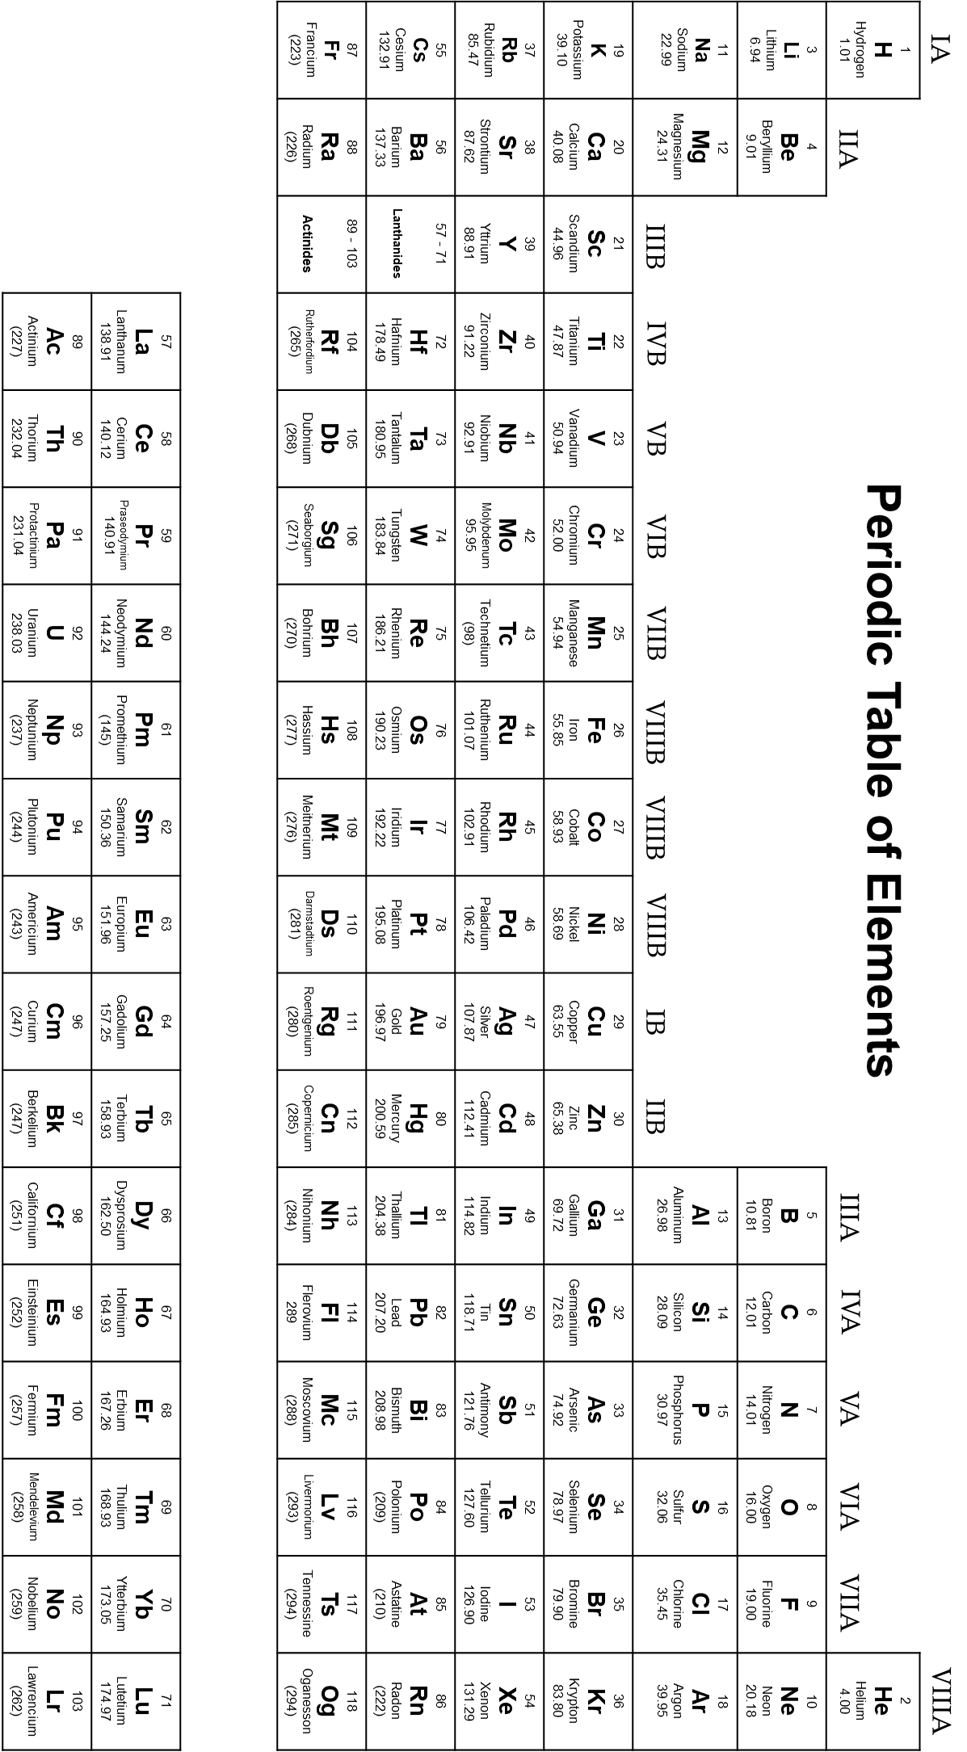
\includegraphics[width=0.75\textwidth]{periodic.png}

% ADD: Periodic Trends, Periods, Collums, Atomic Radius, Electronegativity,

\pagebreak
There is a square for each element. In the middle, you can see the atomic
symbol and the name of the element. In the upper-right corner is the
atomic number --- the number of protons in the atom.

In the upper-left corner is the atomic mass in atomic mass units.\index{atomic mass}

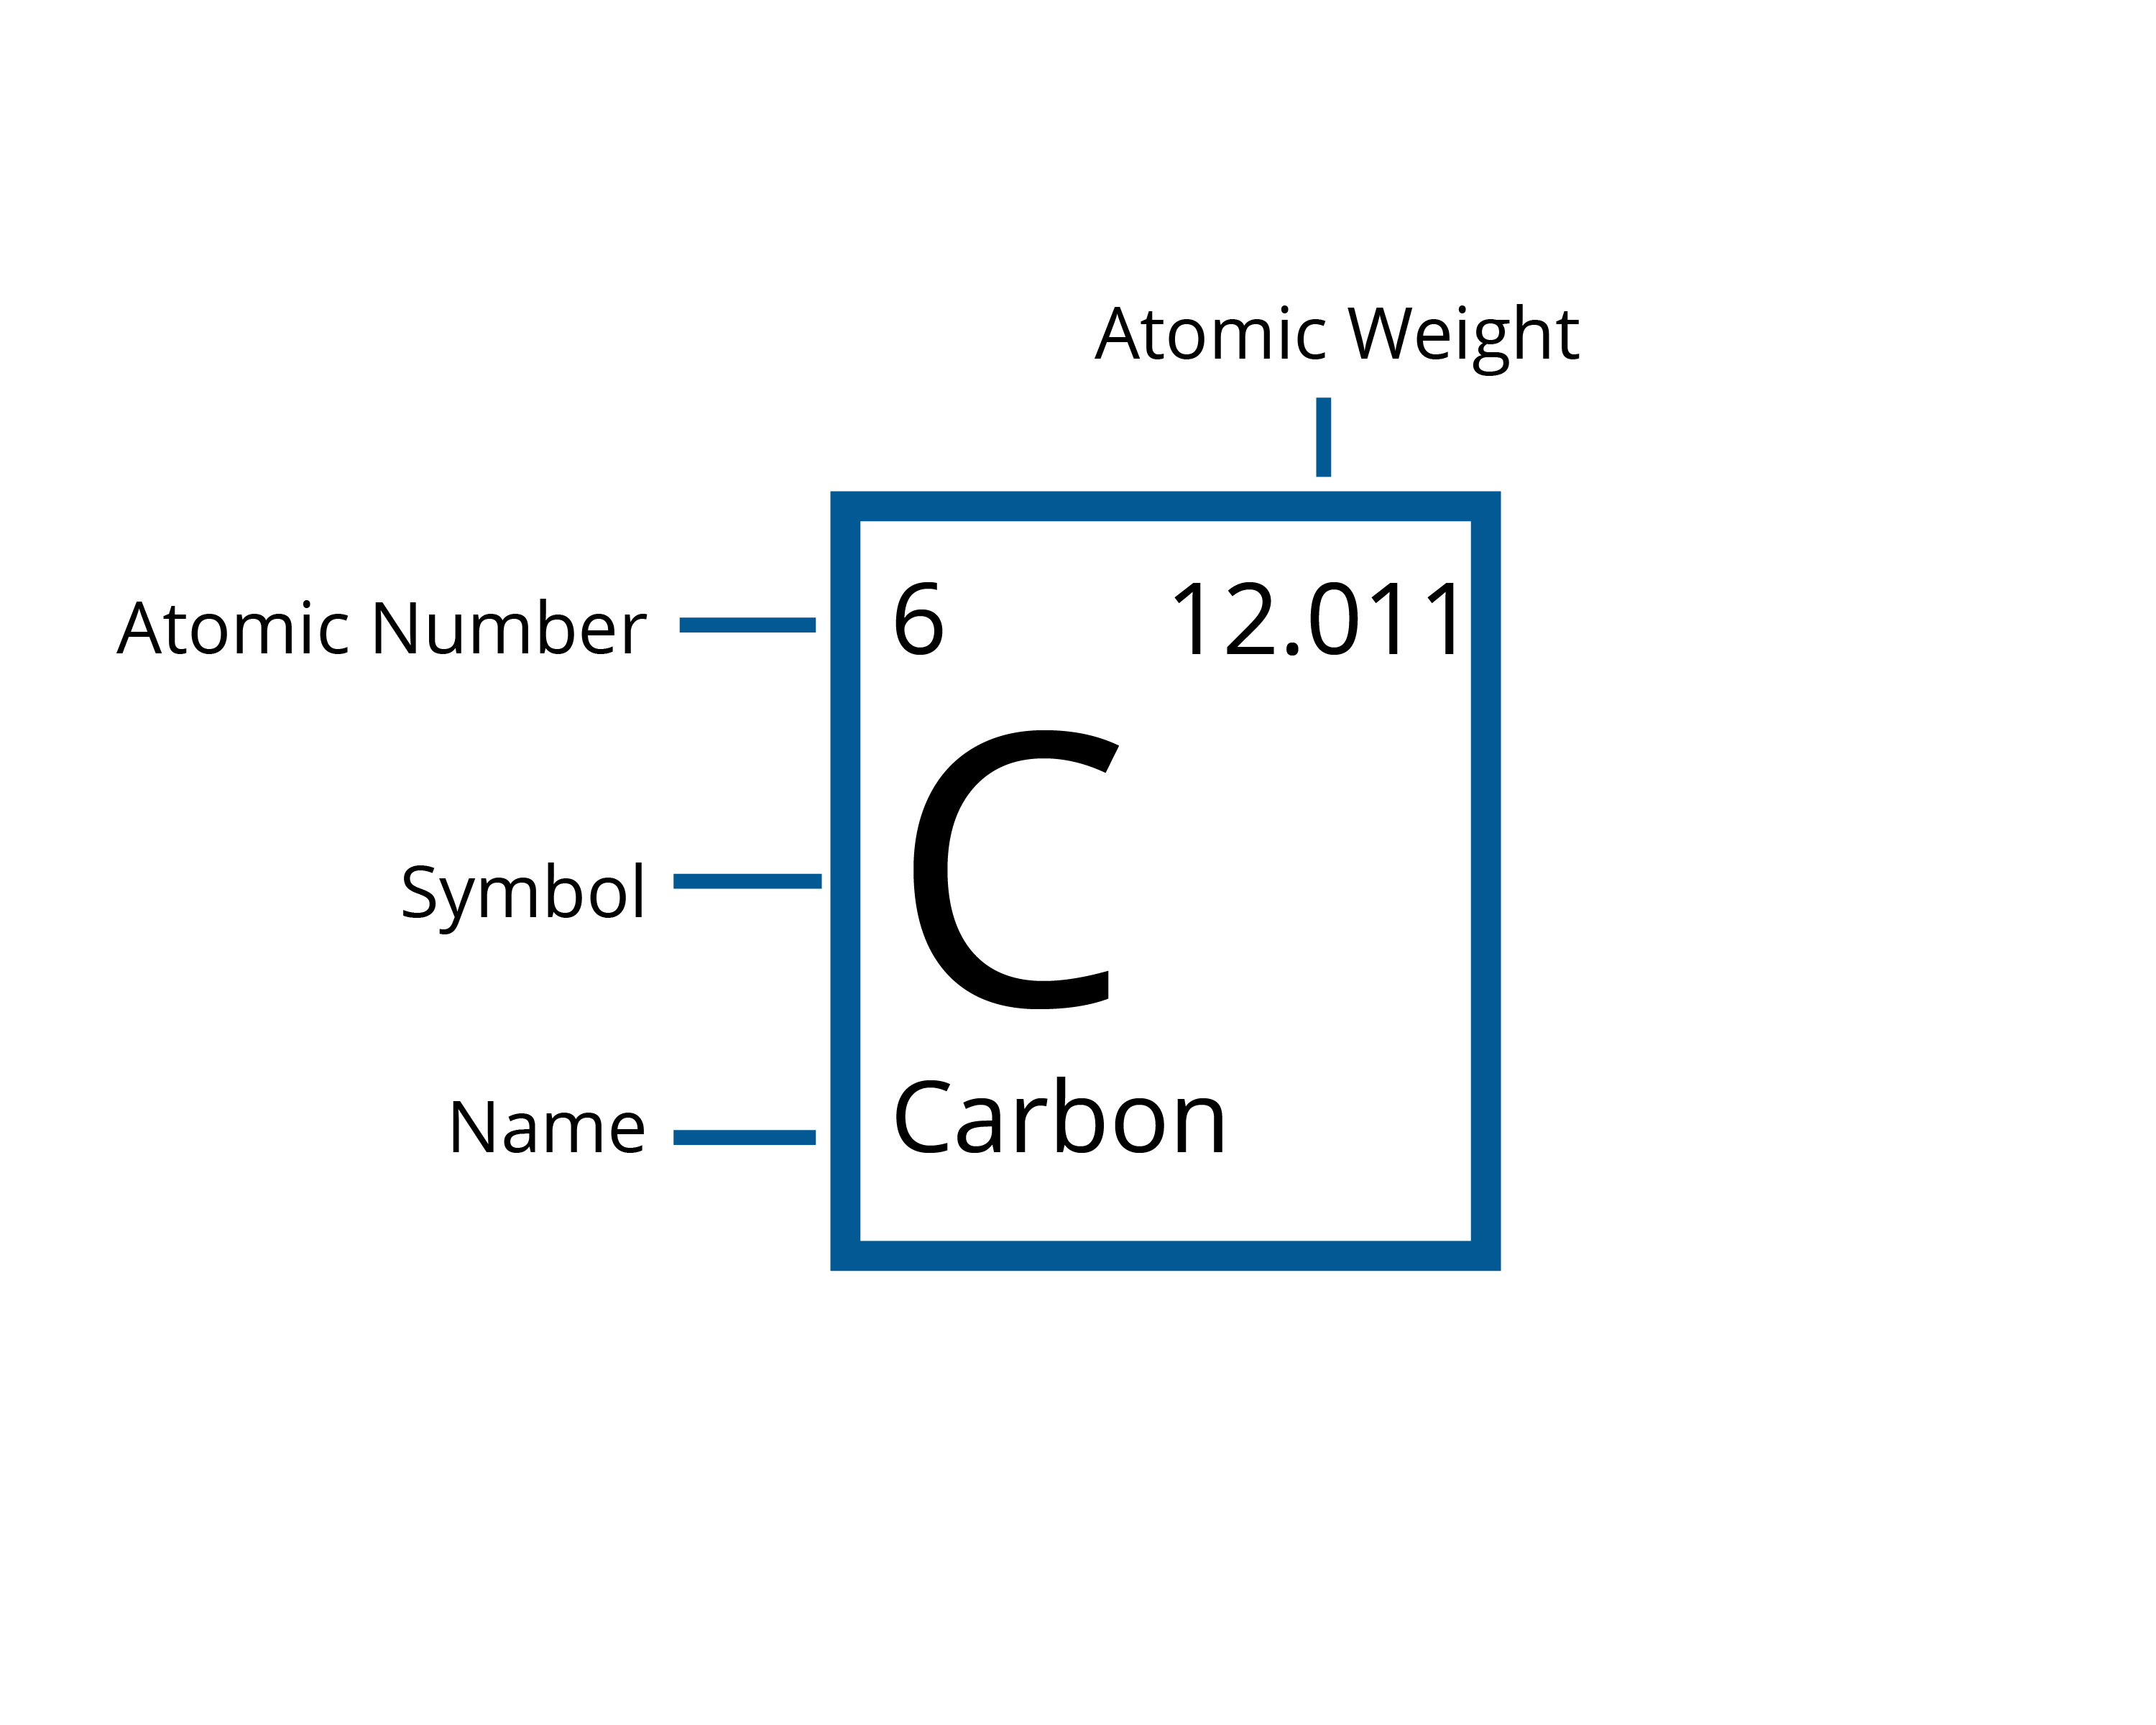
\includegraphics[width=0.8\textwidth]{element.png}

Look at the atomic mass of boron. About 80\% of all boron atoms have
six neutrons. The other 20\% have only 5 neutrons. This difference is why most boron atoms
have a mass of about 11 atomic mass units, but some have a mass of
about 10 atomic mass units. The atomic mass of boron is equivalent to the average
mass of a boron atom: 10.811.
% ADD: Talk about mass spectroscopy
%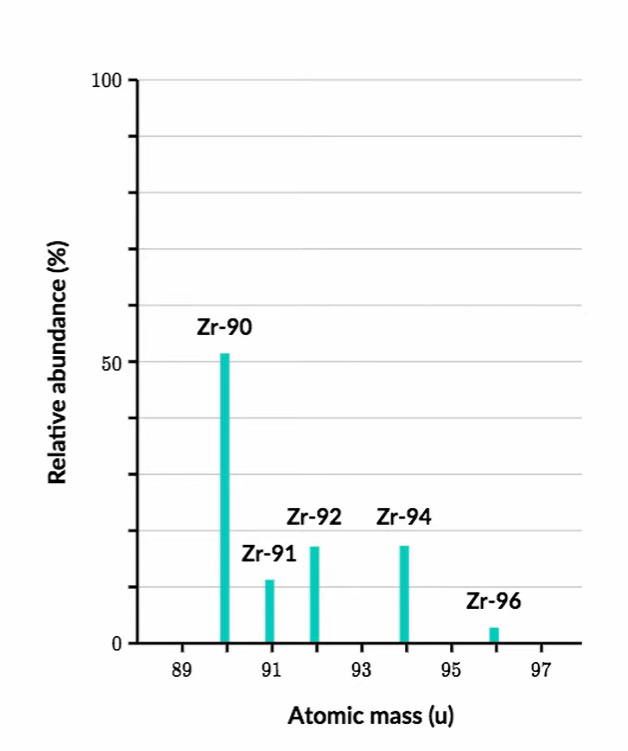
\includegraphics[width=0.75\textwidth]{KA_Mass_Spectroscopy_Zr.png}

\begin{Exercise}[title={Mass of a Water Molecule}, label=water_mass]

Using the periodic table, what is the average mass of one water molecule in atomic mass units?

\end{Exercise}
\begin{Answer}[ref=water_mass]

  The average hydrogen atom has a mass of 1.00794 atomic mass units.

  The average oxygen atom has a mass of 15.9994.

  $2 \times 1.00794 + 15.9994 = 18.01528$ atomic mass units.

\end{Answer}

\section{xfer from intro chapter} 
fixme integrate into this chapter
\subsection{Reading the Periodic Table}
The Periodic Table organizes what we know about the structure of different
elements. Each element has its own block or tile on the Periodic Table, and the
information on the tile tells us about the structure of that atom. Take a look at
the tile for carbon:

\begin{center}
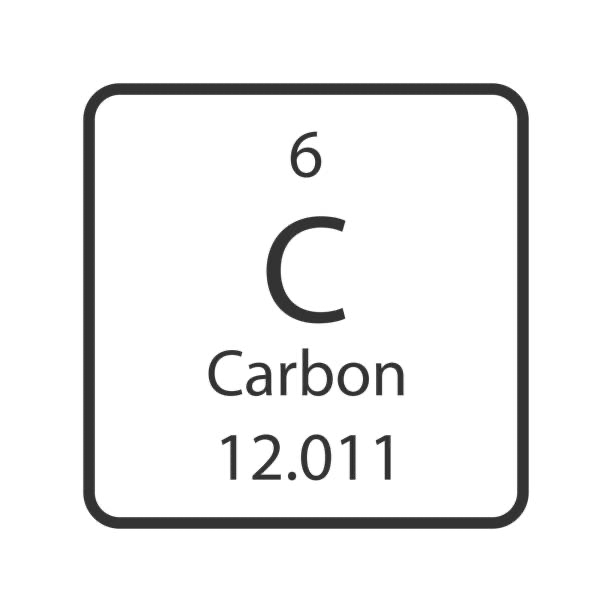
\includegraphics[width=2in]{carbon_tile.png}
\end{center}

The letter (or letters, as is the case for other elements) is the atomic symbol
for the element. There are two key numbers: the atomic number and the average
atomic mass. For carbon, the atomic number is 6 and the average atomic mass is
12.011. The atomic number tells us how many protons there are in the nucleus of
any atom of carbon. Since every element has a unique number of protons, every
element has a unique atomic number. All carbon atoms have 6 protons. The other
number is the average atomic mass - it tells us the weighted average of the
mass of all the carbons in the universe. When the average atomic mass is in
a whole number, as it is for polonium, it means that the element is very unstable.
As a result, the mass given is the mass of the most stable isotope (we'll talk
more about stability and isotopes below). On some periodic tables, the mass
number of the most stable isotope will be in parentheses or brackets. In
summary, if the larger number is a whole number, it is the mass number; if it
is a decimal (even if the decimal ends in .00), it is the average atomic mass,
which we will discuss further below.

\begin{center}
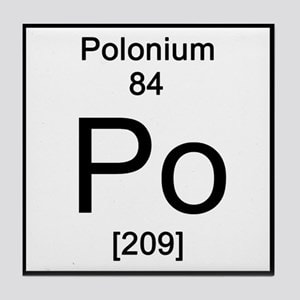
\includegraphics[width=2in]{polonium_tile.png}
\end{center}

The Royal Society of Chemistry has a very useful interactive periodic table:
periodic-table.rsc.org. We can use the periodic tile for an element to
determine the number of protons, electrons, and most common number of neutrons
for a neutral atom of that element (we'll explain why the periodic tile tells
us the "most common number of neutrons" below).

\textbf{Example}: State the atomic symbol for and the number of protons,
neutrons, and electrons in a neutral atom of plutonium.

\textbf{Solution}: The plutonium tile on your periodic table should look
something like this:
\begin{center}
   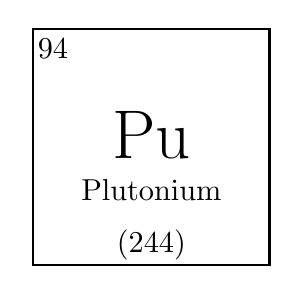
\begin{tikzpicture}
        \draw[black, thick] (-1.5, -1.5) rectangle (1.5,1.5);
        \node[font = \Huge] at (0,0.15) {Pu};
        \node[] at (-1.25, 1.25) {$94$};
        \node[] at (0, -0.55) {Plutonium};
        \node[] at (0, -1.25) {$(244)$};
    \end{tikzpicture}
\end{center}

[The information may be arranged differently, but you should at least see the
symbol and two numbers.] As you can see, the atomic symbol for plutonium is Pu.
Since its atomic number is 94, we know every atom of plutonium has 94 protons.
To know the number of electrons, we will take advantage of the fact that the
question is asking about a \textit{neutral} atom. This means there are the same
number of positive charges as negative charges. So, since there are 94 protons,
a neutral atom of plutonium must have 94 electrons (each proton has a +1 charge
and each electron has a -1 charge). Lastly, let's determine the number of
neutrons. The other number, 244, is the mass number. It represents the total
number of protons and neutrons in the nucleus. Since we know plutonium has 94
protons, we can find the number of neutrons by subtracting the atomic number
from the mass number:

\begin{center}
   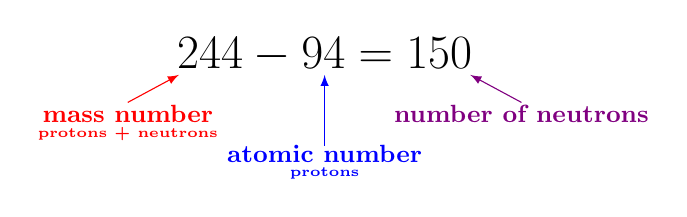
\begin{tikzpicture}
        \node[font = \LARGE] at (0,0) {$244 - 94 = 150$};
        \node[font = \small, red] at (-2.5, -0.75) {\textbf{mass number}};
        \node[font = \tiny, red] at (-2.5, -1) {\textbf{protons + neutrons}};
        \draw[red, -latex] (-2.5, -0.6) -- (-1.85, -0.25);
        \node[font = \small, blue] at (0, -1.25) {\textbf{atomic number}};
        \node[font = \tiny, blue] at (0, -1.5) {\textbf{protons}};
        \draw[blue, -latex] (0, -1.15) -- (0, -0.25);
        \node[font = \small, violet] at (2.5, -0.75) {\textbf{number of neutrons}};
        \draw[violet, -latex] (2.5, -0.6) -- (1.85, -0.25);
    \end{tikzpicture}
\end{center}

Therefore, an atom of plutonium has 150 neutrons. Now let's address how to find
the number of neutrons when the periodic tile shows an average atomic mass,
instead of a mass number. This occurs when there is more than one "version" of
an element. In the case of plutonium, there is only one version, which is why
the periodic tile shows a mass number instead of an average atomic mass. To
learn about average atomic mass, we will use carbon as an example.

Have you heard of carbon-14 dating? The phrase "carbon-14" refers to a rare
type of carbon that decays radioactively. By seeing how much carbon-14 has
decayed, scientists can estimate the age of organic materials, such as bone or
ash. Carbon-14 is a radioactive isotope (or version) of carbon. The 14 refers to
the mass number - the total amount of protons and neutrons in the nucleus
(sometimes, we shorten the isotope name by just using the atomic symbol, in
this case C-14). Isotopes are versions of an element with different numbers of
neutrons. The atomic number is the same for them all - they all have the same
number of protons. But the different number of neutrons causes different
isotopes to have different masses. Examine the models of carbon-12, carbon-13,
and carbon-14 below. What is different between them? What is the same?



You should have noticed that all three atoms have 6 protons and 6 electrons,
while they have differing numbers of neutrons. The most common isotope of carbon
is carbon-12, with 6 protons and 6 neutrons in its nucleus. Carbon-14, on the
other hand, has 8 neutrons, which makes the nucleus unstable, leading to
radioactive decay. The average atomic mass
is the weighted average of all the carbon atoms in existence. Since the vast
majority of carbon is carbon-12, the average atomic mass is very close to 12.
You cannot determine the mass number of an individual atom from the periodic
table; it only tells you the average of all the isotopes. However, especially
for light atoms (atoms in the first two rows of the periodic table), you can
usually determine the mass number of the most common isotope by rounding the
average atomic mass to the nearest whole number.

\textbf{Example}: Germanium has atomic symbol Ge. State the number of protons,
number of electrons, and most common number of neutrons in a neutral atom of
germanium.

\textbf{Solution}: Examining the periodic table, we see that germanium has an
atomic number of 32, which means a neutral atom of germanium has 32 protons and
32 electrons. The average atomic mass is 72.630, which rounds up to 73. So, the
most common isotope of germanium is Ge-73, which has $73 - 32 = 41$ neutrons.

\begin{Exercise}[title = {Determining Numbers of Subatomic Particles}, label = pne]
Use a periodic table to complete the table below (assume neutral atoms): %fixme wrap text for neutrons column

\begin{tabular}{|c|c|c|c|c|}
\hline\\
Element Name & Atomic Symbol & Protons & Most Common Number of Neutrons & Electrons\\\hline
 & Fr & & & \\\hline
 & & & & 33\\\hline
 Erbium & & & & \\\hline
  & & 48 & & \\\hline
\end{tabular}
\end{Exercise}

\begin{Answer}[ref = pne]
\begin{tabular}{|c|c|c|c|c|}
\hline\\
Element Name & Atomic Symbol & Protons & Most Common Number of Neutrons & Electrons\\\hline
 Francium & Fr & 87 & 136 & 87 \\\hline
 Arsenic & As & 33 & 42 & 33 \\\hline
 Erbium & Er & 68 & 99 & 68 \\\hline
 Cadmium & Cd & 48 & 64 & 48 \\\hline
\end{tabular}
\end{Answer}




\section{Heavy atoms aren't stable}

When you look at the periodic table, there are a surprisingly large
number of elements. You might be told to ``Drink milk so that you can
get the calcium you need.'' However, no one has told you ``You should
eat kale so that you get enough copernicium in your diet.''

Copernicium, with 112 protons and 173 neutrons, has only been observed
 in a lab. It is highly radioactive and unstable (meaning it decays). A copernicium
atom usually lives for less than a minute before decaying.
% ADD: Half Life

The largest stable element is lead, which has 82 protons and between
122 and 126 neutrons. Elements with lower atomic numbers than lead,
have at least one stable isotope, while elements with higher atomic numbers
than lead don't.

Bismuth, with an atomic number of 83, is \textit{almost} stable. In fact, most
bismuth atoms will live for billions of years before decaying!

\graphicspath{{../../Chapters/work_energy/en_US}}
\chapter{Work and Energy}

In this chapter, we are going to talk about how engineers define work
and energy. It frequently takes force to get work done. Let's start with thinking about the relationship between force and energy. As we learned earlier, Force is measured in
newtons, and one newton is equal to the force necessary to accelerate one
kilogram at a rate of $1 m/s^2$.

When you lean on a wall, you are exerting a force on the wall, but you
aren't doing any work. On the other hand, if you push a car for a mile,
you are clearly doing work. Work, to an engineer, is the force you
apply to something, as well as the distance that it moves, in the direction
of the applied force. We measure work in \textit{joules}. A joule is one
newton of force over one meter.\index{Joule}

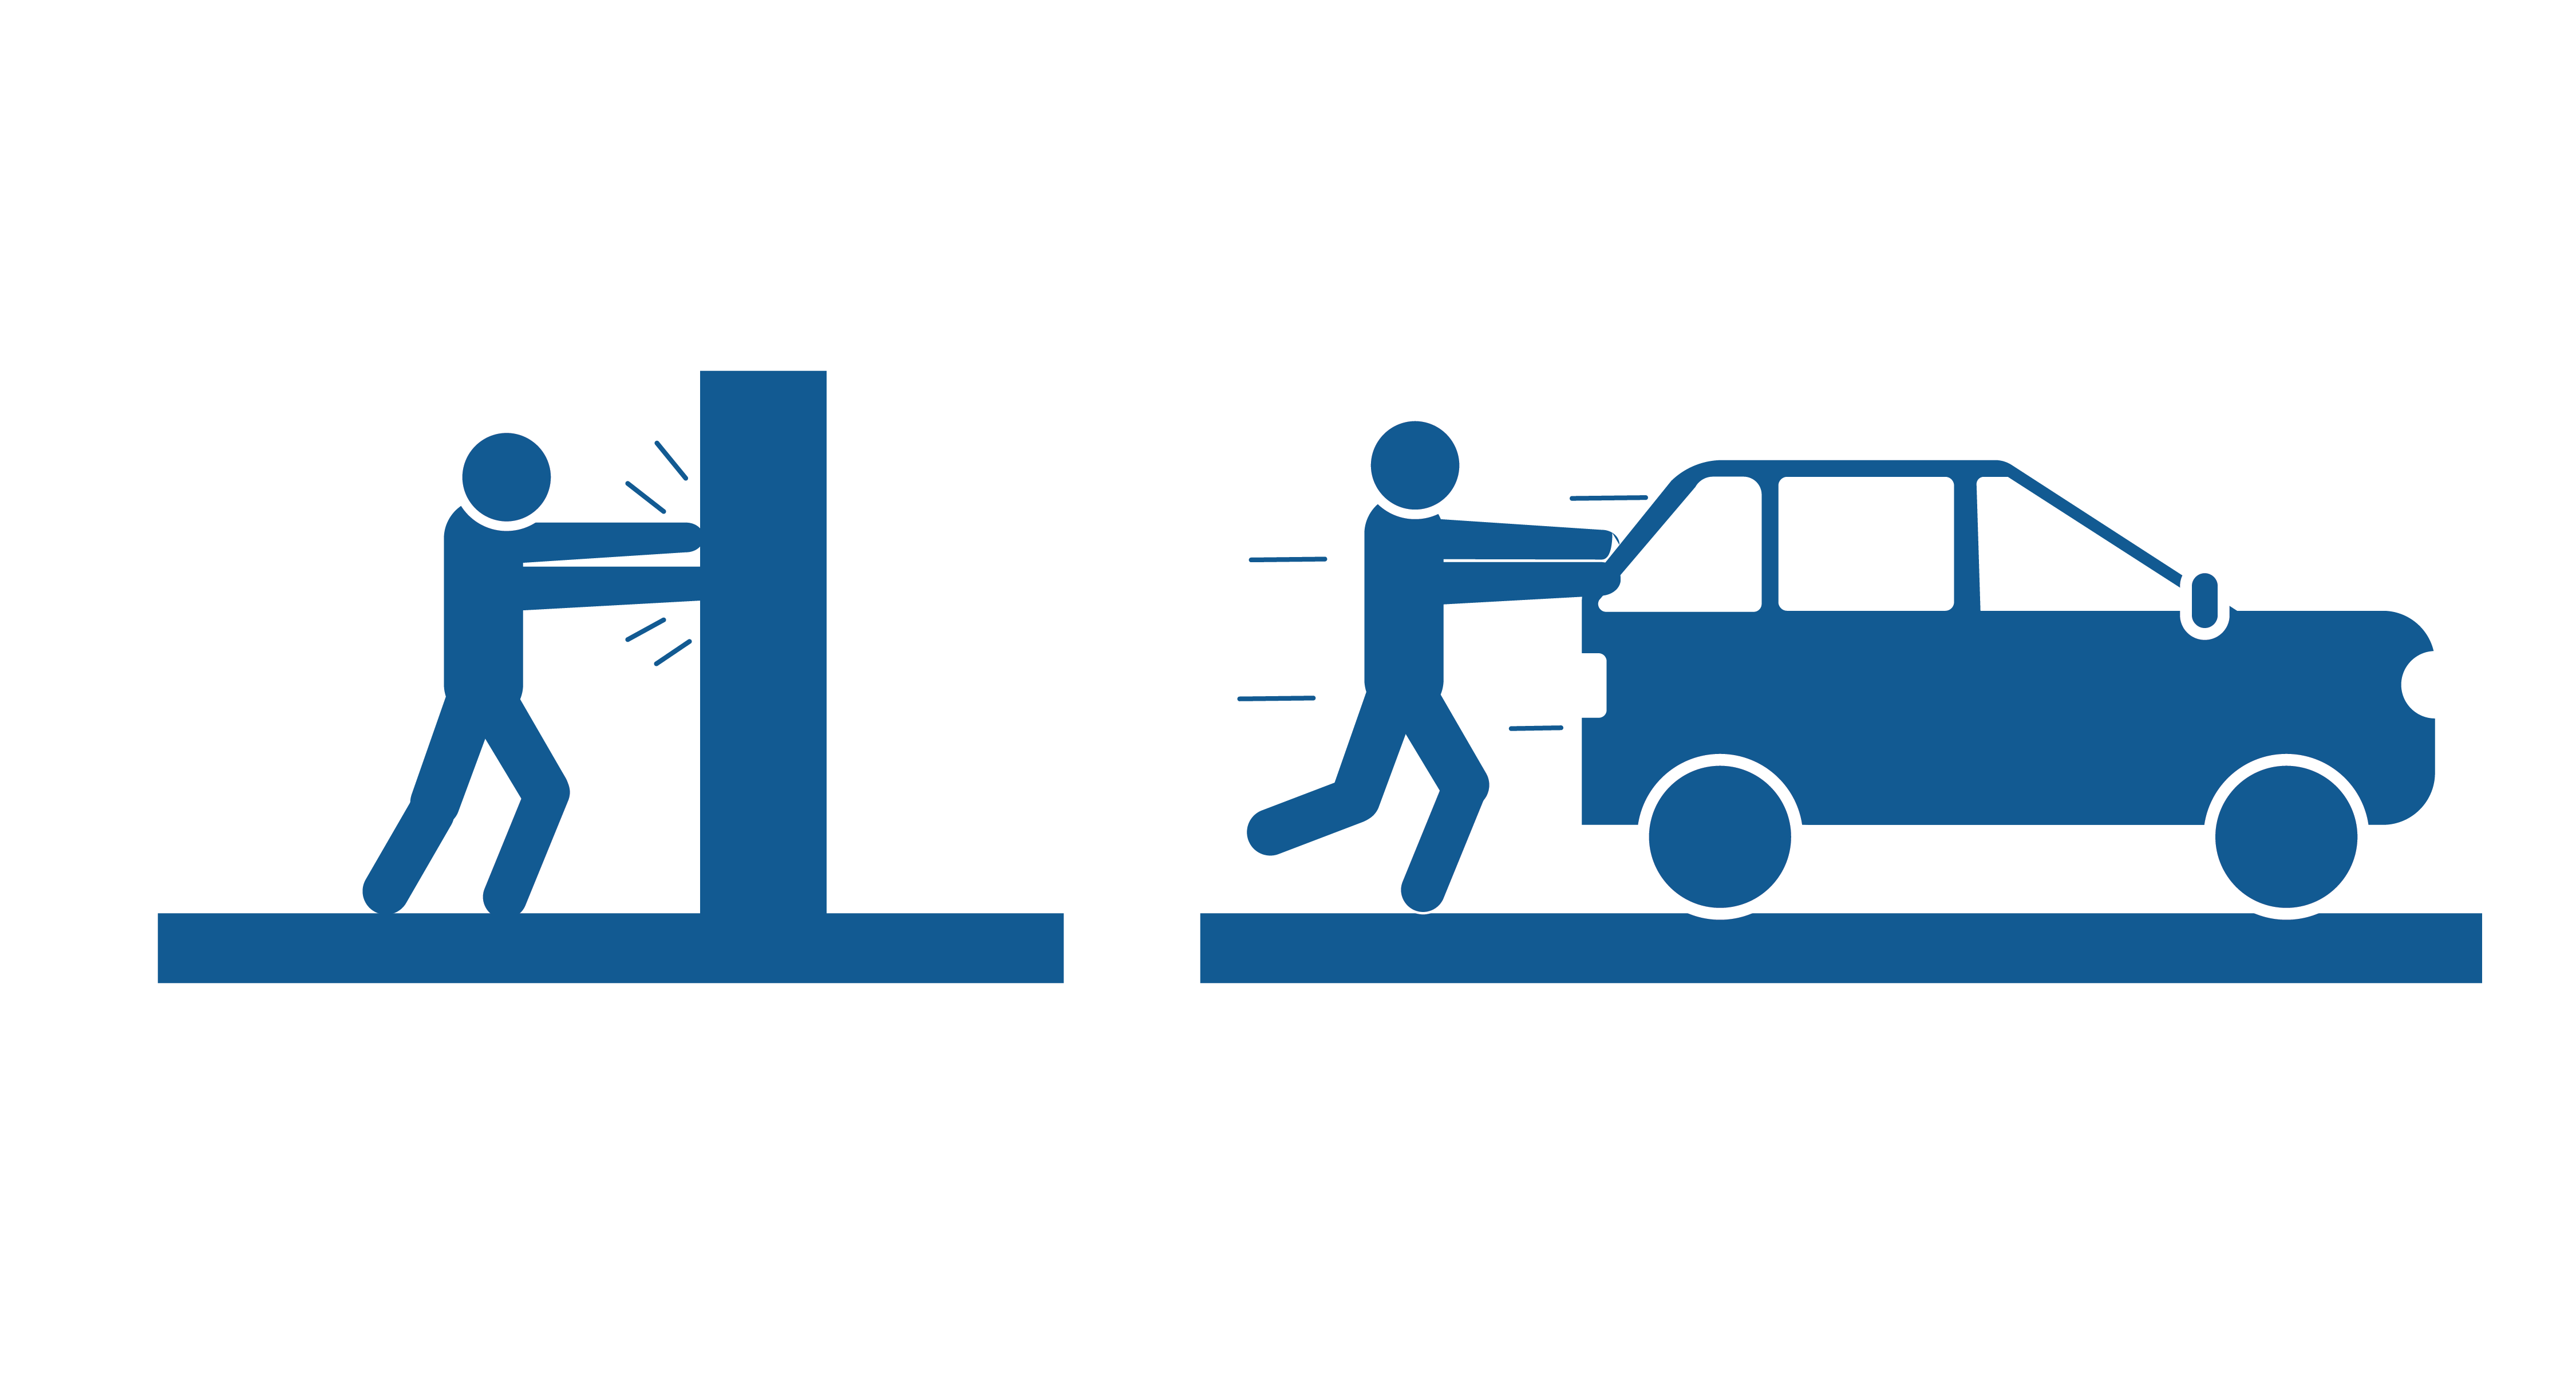
\includegraphics[width=1\textwidth]{workvsforce.png}

For example, if you push a car uphill with a force of 10 newtons for 12
meters, you have done 120 joules of work.\index{work}
% ADD: We can represent this with the equations, Work Energy Therom

Work is how energy is transferred from one thing to another. When you
push the car, you also burn sugars(energy of the body) in your blood. That energy is then
transferred to the car: after it has been pushed uphill.

Thus, we measure the energy something consumes or generates in 
units of work: joules, kilowatt-hours, horsepower-hours, foot-pounds,
BTUs( British Thermal Unit), and calories.

Let's go over a few different forms that energy can take.

Watch Khan Academy's \textbf{Changes in energy} at \url{https://www.khanacademy.org/science/ms-physics/x1baed5db7c1bb50b:energy/x1baed5db7c1bb50b:changes-in-energy/a/changes-in-energy}

\section{Forms of Energy}\index{energy!Forms of}

In this section we are going to learn about several different types of energy:
\begin{itemize}
\item Heat
\item Chemical Energy
\item Kinetic Energy
\item Gravitational Potential Energy
\end{itemize}

\subsection{Heat}\index{heat}

When you heat something, you are transferring energy to it. The BTU
 is a common unit for heat: One BTU is the
amount of heat required to raise the temperature of one pound of water,
by one degree. One BTU is about 1,055 joules. In fact, when you buy and sell
natural gas as fuel, it is priced by the BTU.\index{heat} \index{BTU}

\subsection{Electricity}\index{electricity}

Electricity is the movement of electrons. When you push electrons
through a space that resists their passage (like a light bulb),
energy is transferred from the power source ( a battery)
 into the source of the resistance.

Let's say your lightbulb consumes 60 watts of electricity, and you leave it on for 24 hours.
We would say that you have consumed 1.44 kilowatt hours or 3,600,000 joules.

Watch Khan Academy's \textbf{Introduction to charge} at \url{https://www.khanacademy.org/science/in-in-class10th-physics/in-in-electricity/in-in-electric-current-circuit/v/intro-to-charge}

\subsection{Chemical Energy}\index{chemical energy}

As mentioned early, some chemical reactions consume energy and some
produce energy. Thus, energy can be stored in the structure of a
molecule. When a plant uses photosynthesis to rearrange water and
carbon dioxide into a sugar molecule, it converts the energy in
the sunlight( solar energy) into chemical energy. Remember photosythesis is a process that releases energy.
Therefore, the sugar molecule has more chemical energy than the carbon dioxide and water molecules that were
used in its creation.
% ADD: photosythesis equation 
% KA: https://www.khanacademy.org/science/ap-biology/cellular-energetics/photosynthesis/a/intro-to-photosynthesis

In our diet, we measure this energy in \textit{kilocalories}. A
calorie is the energy necessary to raise one gram of water one degree
Celsius: it is about 4.19 joules. This is a very small unit: an apple
has about 100,000 calories( 100 kilocalories), so people working with food started
measuring everything in kilocalories.\index{calories}
% ADD: Conversion chapter should come before this chapter

Here is where things get confusing: People who work with food got tired of
saying ``kilocalories'', so they just started using ``Calorie'' to
mean 1,000 calories.  This has created terrible confusion over the
years. So if the C is capitalized, ``Calorie'' probably means kilocalorie.

\subsection{Kinetic Energy}\index{kinetic energy}

A mass in motion has energy. For example, if you are in a moving car
and you slam on the breaks, the energy from the motion of the
car will be converted into heat in the breaks and under the tires.

How much energy does the car have?
% ADD: section specifically about KE AND U, use roller coaster diagram

\begin{mdframed}[style=important, frametitle={Formula for Kinetic Energy}]

$$E = \frac{1}{2} m v^2$$

where $E$ is the energy in joules, $m$ is the mass in kilograms, and
$v$ is the speed in meters per second.

\end{mdframed}

\subsection{Gravitational Potential Energy}\index{potential energy!gravitational}

Watch Khan Academy's \textbf{Potential energy} at \url{https://youtu.be/oGzwVYPxKjg}

When you lift something heavy onto a shelf, you are giving it
\textit{potential energy}. The amount of energy that you transferred
to it is proportional to its weight and the height that you lifted it.

On the surface of the earth, gravity will accelerate a heavy object downward at
a rate of $9.8 m/s^2$.

\begin{mdframed}[style=important, frametitle={Formula for Gravitational Potential Energy}]
On earth, then, gravitational potential energy is given by

$$E = (9.8)mh$$


where $E$ is the energy in joules, $m$ is the mass of the object you
lifted, and $h$ is the height that you lifted it.

\end{mdframed}


There are other kinds of potential energy. For example, when you draw
a bow, you have given that bow potential energy. When you release it,
the potential energy is transferred to the arrow, which expresses it
as kinetic energy.
% ADD: section about KE and U

\section{Conservation of Energy}

The first law of thermodynamics says ``Energy is neither created nor
destroyed.''\index{energy!conservation of}

Energy can change forms: Your cells consume chemical energy to give
gravitational potential energy to a car you push up a hill. However, the total amount of
energy in a closed system stays constant.
% ADD: Create Systems chapter before introducing concept here

\begin{Exercise}[title={The Energy of Falling}, label=energy_falling]
  
A 5 kg cannonball falls off the top of a 3 meter ladder. Just before
it hits the floor, all of its gravitational potential energy has been
converted into kinetic energy.  How fast is the cannonball going when
it hits the floor?

\end{Exercise}
\begin{Answer}[ref=energy_falling]

  At the top of the ladder, the cannonball has $(9.8)(5)(3) = 147$ joules of potential energy.

  At the bottom, the kinetic energy $\frac{1}{2}(5)v^2$ must be equal
  to 147 joules. So $v^2 = \frac{294}{5}$.  Thus it is going about
  $7.7$ meters per second.

  (Yes, a tiny amount of energy is lost to air resistance. For a dense
  object moving at these relatively slow speeds, this energy is
  neglible.)
  
\end{Answer}


\section{Efficiency}


Watch Khan Academy's \textbf{Laws of thermodynamics} at \url{https://www.khanacademy.org/science/ap-biology/cellular-energetics/cellular-energy/a/the-laws-of-thermodynamics}

Although energy is always conserved as it moves through different
forms, scientists aren't always that good at controlling it.\index{efficiency}

For example, a car engine consumes the chemical energy in gasoline. Only
about 20\% of the energy consumed is used to turn the wheels.  Most of
the energy is actually lost as heat. If you run a car for a while, the engine
gets very hot and the exhaust going out the tailpipe turns hot.

A human is about 25\% efficient. Most of the loss is in the heat produced
during the chemical reactions that turns food into motion.
% ADD: Cellular Respiration
 
In general, if you are trying to increase efficiency in any system,
the solution is usually easy to identify because heat is produced. Reduce heat, Increase efficiency.

Light bulbs are an interesting case. To get the light of a 60 watt
incandescent bulb, you can use an 8 watt LED or a 16 watt fluorescent
light. Thus, we say that the LED light is much more efficient: If you
run both, the incandescent bulb will consume 1.44 kilowatt-hours. The
LED will consume only 0.192 kilowatt-hours.

Besides light, the incandescent bulb is producing a lot of heat. If it
is inside your house, what happens to the heat? It warms your house.

In the winter, when you want light and heat, the incandescent bulb is
100\% efficient!

In the summer, if you are running the air conditioner, the
incandescent bulb is worse than just ``inefficient at making light'' --
it is actually counteracting the air conditioner! 


\graphicspath{{../../Chapters/units_conversions/en_US}}
\chapter{Units and Conversions}

At this point, you are working with a lot of units: grams for weight,
joules for energy, newtons for force, meters for distance, seconds for
time, etc. For each type of measurement, there are several different
units; for example, distance can be measured in feet, miles,
and light-years.

\begin{mdframed}[style=important, frametitle={Some Equalencies}]

\begin{tabular}{r | l}
  \hline
  \multicolumn{2}{c}{\textbf{Distance}}\\
  1 mile & 1.6093 kilometers \\
  1 foot & 0.3048 meters \\
  1 inch & 2.54 centimeters \\
  1 light-year & $9.461 \times 10^{12}$ kilometers\\
  \hline
  \multicolumn{2}{c}{\textbf{Volume}}\\
  1 milliliter & 1 cubic centimeter \\
  1 quart & 0.9461 liters \\
  1 gallon & 3.7854 liters \\
  1 fluid ounce & 29.6 milliliters \\
  \hline
  \multicolumn{2}{c}{\textbf{Mass}}\\
  1 pound & 0.4535924 kilograms\\
  1 ounce & 0.4535924 grams\\
  1 metric ton & 1000 kilograms \\
  \hline
  \multicolumn{2}{c}{\textbf{Force}}\\
  1 newton & 1 kilogram meter per sec$^2$\\
  \hline
  \multicolumn{2}{c}{\textbf{Pressure}}\\
  1 pascal & 1 newton per square meter \\
  1 bar & 0.98692 atmosphere \\
  1 pound per square inch & 6897 pascals \\
  \hline
  \multicolumn{2}{c}{\textbf{Energy}}\\
  1 joule & 1 newton meter \\
  1 calorie & 4.184 joules \\
  1 kilowatt-hour & $3.6 \times 10^{6}$ joules  \\
\end{tabular}\index{units table}

(You don't need to memorize these! Just remember that this page is here.)
% Suggest putting this in the front or back of the book, maybe create a print out

\end{mdframed}

In the metric system, prefixes are often used to express a multiple. Here are the common prefixes:\index{metric system!prefixes}

\begin{mdframed}[style=important, frametitle={Common Prefixes for Metric Units}]

\begin{tabular}{r | l}
giga  & $\times 10^{9}$\\
mega  & $\times 10^{6}$\\
kilo  & $\times 10^{3}$\\
milli  & $\div 10^{3}$\\
micro  & $\div 10^{6}$\\
nano  & $\div 10^{9}$\\
\end{tabular}

(These are worth memorizing. Here's a mnemonic: ``King Henery Doesn't Usually Drink Chocolate Milk.'')
\end{mdframed}

\section{Conversion Factors}

Here is a really handy trick to remembering how to do conversions
between units.\index{conversion factors}

Often, you will be given a table like the one above, and someone will ask you
``How many miles are in 0.23 light-years?''  You know that 1 mile = 1.6093
kilometers and that 1 light-year is $9.461 \times 10^{12}$ kilometers.
How do you do the conversion?

The trick is to treat the two parts of the equality as a fraction that equals 1.  That is, you think:

$$\frac{1 \text{ miles}}{1.6093 \text{ km}} = \frac{1.6093 \text{ km}}{1 \text{ miles}} = 1$$

and

$$\frac{1 \text{ light-years}}{9.461 \times 10^{12} \text{ km}} = \frac{9.461 \times 10^{12} \text{ km}}{1 \text{ light-years}} = 1$$

We call these fractions \textit{conversion factors}.

Now, your problem is

$$0.23 \text{ light-years} \times \textit{ Some conversion factors} = ? \text{ miles}$$

Note that when you multiply fractions together, things in the numerators can cancel with things in the denominator:

$$\left( \frac{31\pi}{47} \right) \left( \frac{11}{37\pi}\right) = \left(\frac{31\cancel{\pi}}{47}\right) \left( \frac{11}{37\cancel{\pi}}\right) = \left(\frac{31}{47} \right) \left( \frac{11}{37} \right)$$

When working with conversion factors, you will do the same with the units:

\begin{multline*}
  0.23 \text{ light-years} \left( \frac{9.461 \times 10^{12} \text{ km}}{1 \text{ light-years}} \right) \left( \frac{1 \text{ miles}}{1.6093 \text{ km}} \right) = \\
  0.23 \text{ \cancel{light-years}} \left( \times \frac{9.461 \times 10^{12} \text{ \cancel{km}}}{1 \text{ \cancel{light-years}}} \right) \left( \frac{1 \text{ miles}}{1.6093 \text{ \cancel{km}}}\right) = \frac{(0.23)(9.461 \times 10^{12})}{1.6093} \text{ miles}$$
\end{multline*}

\begin{Exercise}[title={Simple Conversion Factors}, label=simple_conversion_factors]

  How many calories are in 4.5 kilowatt-hours?
  
\end{Exercise}
\begin{Answer}[ref=simple_conversion_factors]

  $$4.5 \text{ \cancel{kWh}} \left( \frac{3.6 \times 10^{6} \text{ \cancel{joules}}}{1 \text{ \cancel{kWh}}} \right) \left( \frac{1 \text{ calories}}{4.184 \text{ \cancel{joules}}}\right) = \frac{(4.5)(3.6 \times 10^6)}{4.184} = 1.08 \times 10^6 \text {calories}$$
  
\end{Answer}

\section{Conversion Factors and Ratios}

Conversion factors also work on ratios.  For example, if you are told
that a bug is moving 0.5 feet every 120 milliseconds. What is that in
meters per second?

The problem then is

$$\frac{0.5 \text{ feet}}{120 \text{ milliseconds}} = \frac{\text{? m}}{second}$$

So you will need conversion factors to replace the ``feet'' with ``meters'' and to replace ``milliseconds'' with ``seconds'':

\begin{multline*}
\left(\frac{0.5 \text{ \cancel{feet}}}{120 \text{ \cancel{milliseconds}}}\right) \left( \frac{0.3048 \text{ meters}}{1 \text{ \cancel{feet}}} \right) \left( \frac{ 1000 \text{ \cancel{milliseconds}}} {1 \text{ second}}\right) = \frac{(0.5)(0.3048)(1000)}{120}\text{ m/second}
\end{multline*}

\begin{Exercise}[title={Conversion Factors}, label=conversion_factors]

The hole in the bottom of the boat lets in 0.1 gallons every 2 minutes.  How many milliliters per second is that?
  
\end{Exercise}
\begin{Answer}[ref=onversion_factors]

  \begin{multline*}
    \frac{0.1 \text{ \cancel{gallons}}}{2 \text{ \cancel{minutes}}}
  \left( \frac{3.7854 \text{ \cancel{liters}}}{1 \text{ \cancel{gallons}}} \right)
  \left( \frac{1000 \text{ milliliters}}{1\text{ \cancel{liters}}}\right)
  \left( \frac{1 \text{ \cancel{minutes}}}{60 \text{ seconds}} \right) = \\
  \frac{(0.1)(3.7854)(1000)}{(2)(60)} \text{ ml/second} = 3.1545 \text{ ml/second}
  \end{multline*}
  
\end{Answer}

\section{When Conversion Factors Don't Work}

Conversion factors only work when the units being converted are
proportional to each other. Gallons and liters, for example, are
proportional to each other: If you have $n$ gallons, you have $n
\times 3.7854$ liters.

Degrees celsius and degrees farenheit are \textit{not} proportional to
each other.  If your food is $n$ degrees celsius, it is $n \times
\frac{9}{5} + 32$ degrees farenheit.  You can't use conversion factors
to convert celsius to farenheit.

Watch Khan Academy's video on this at \url{https://www.khanacademy.org/test-prep/sat/x0a8c2e5f:untitled-652/x0a8c2e5f:problem-solving-and-data-analysis-lessons-by-skill/a/gtp--sat-math--article--units--lesson}


\graphicspath{{../../Chapters/simple_machines/en_US}}
\chapter{Simple Machines}

As mentioned earlier, physicists define work as the force applied times the distance over which it is applied. For example, if you push your car 100 meters with a force of 17 newtons, you have done 1700 joules of work.

Humans have long needed to move heavy objects, so many centuries ago, we developed simple machines to reduce the amount of force necessary to perform such tasks. These include:

\begin{itemize}
    \item Levers
    \item Pulleys
    \item Inclined planes
    \item Gears
    \item Hydraulics
    \item Screws
\end{itemize}

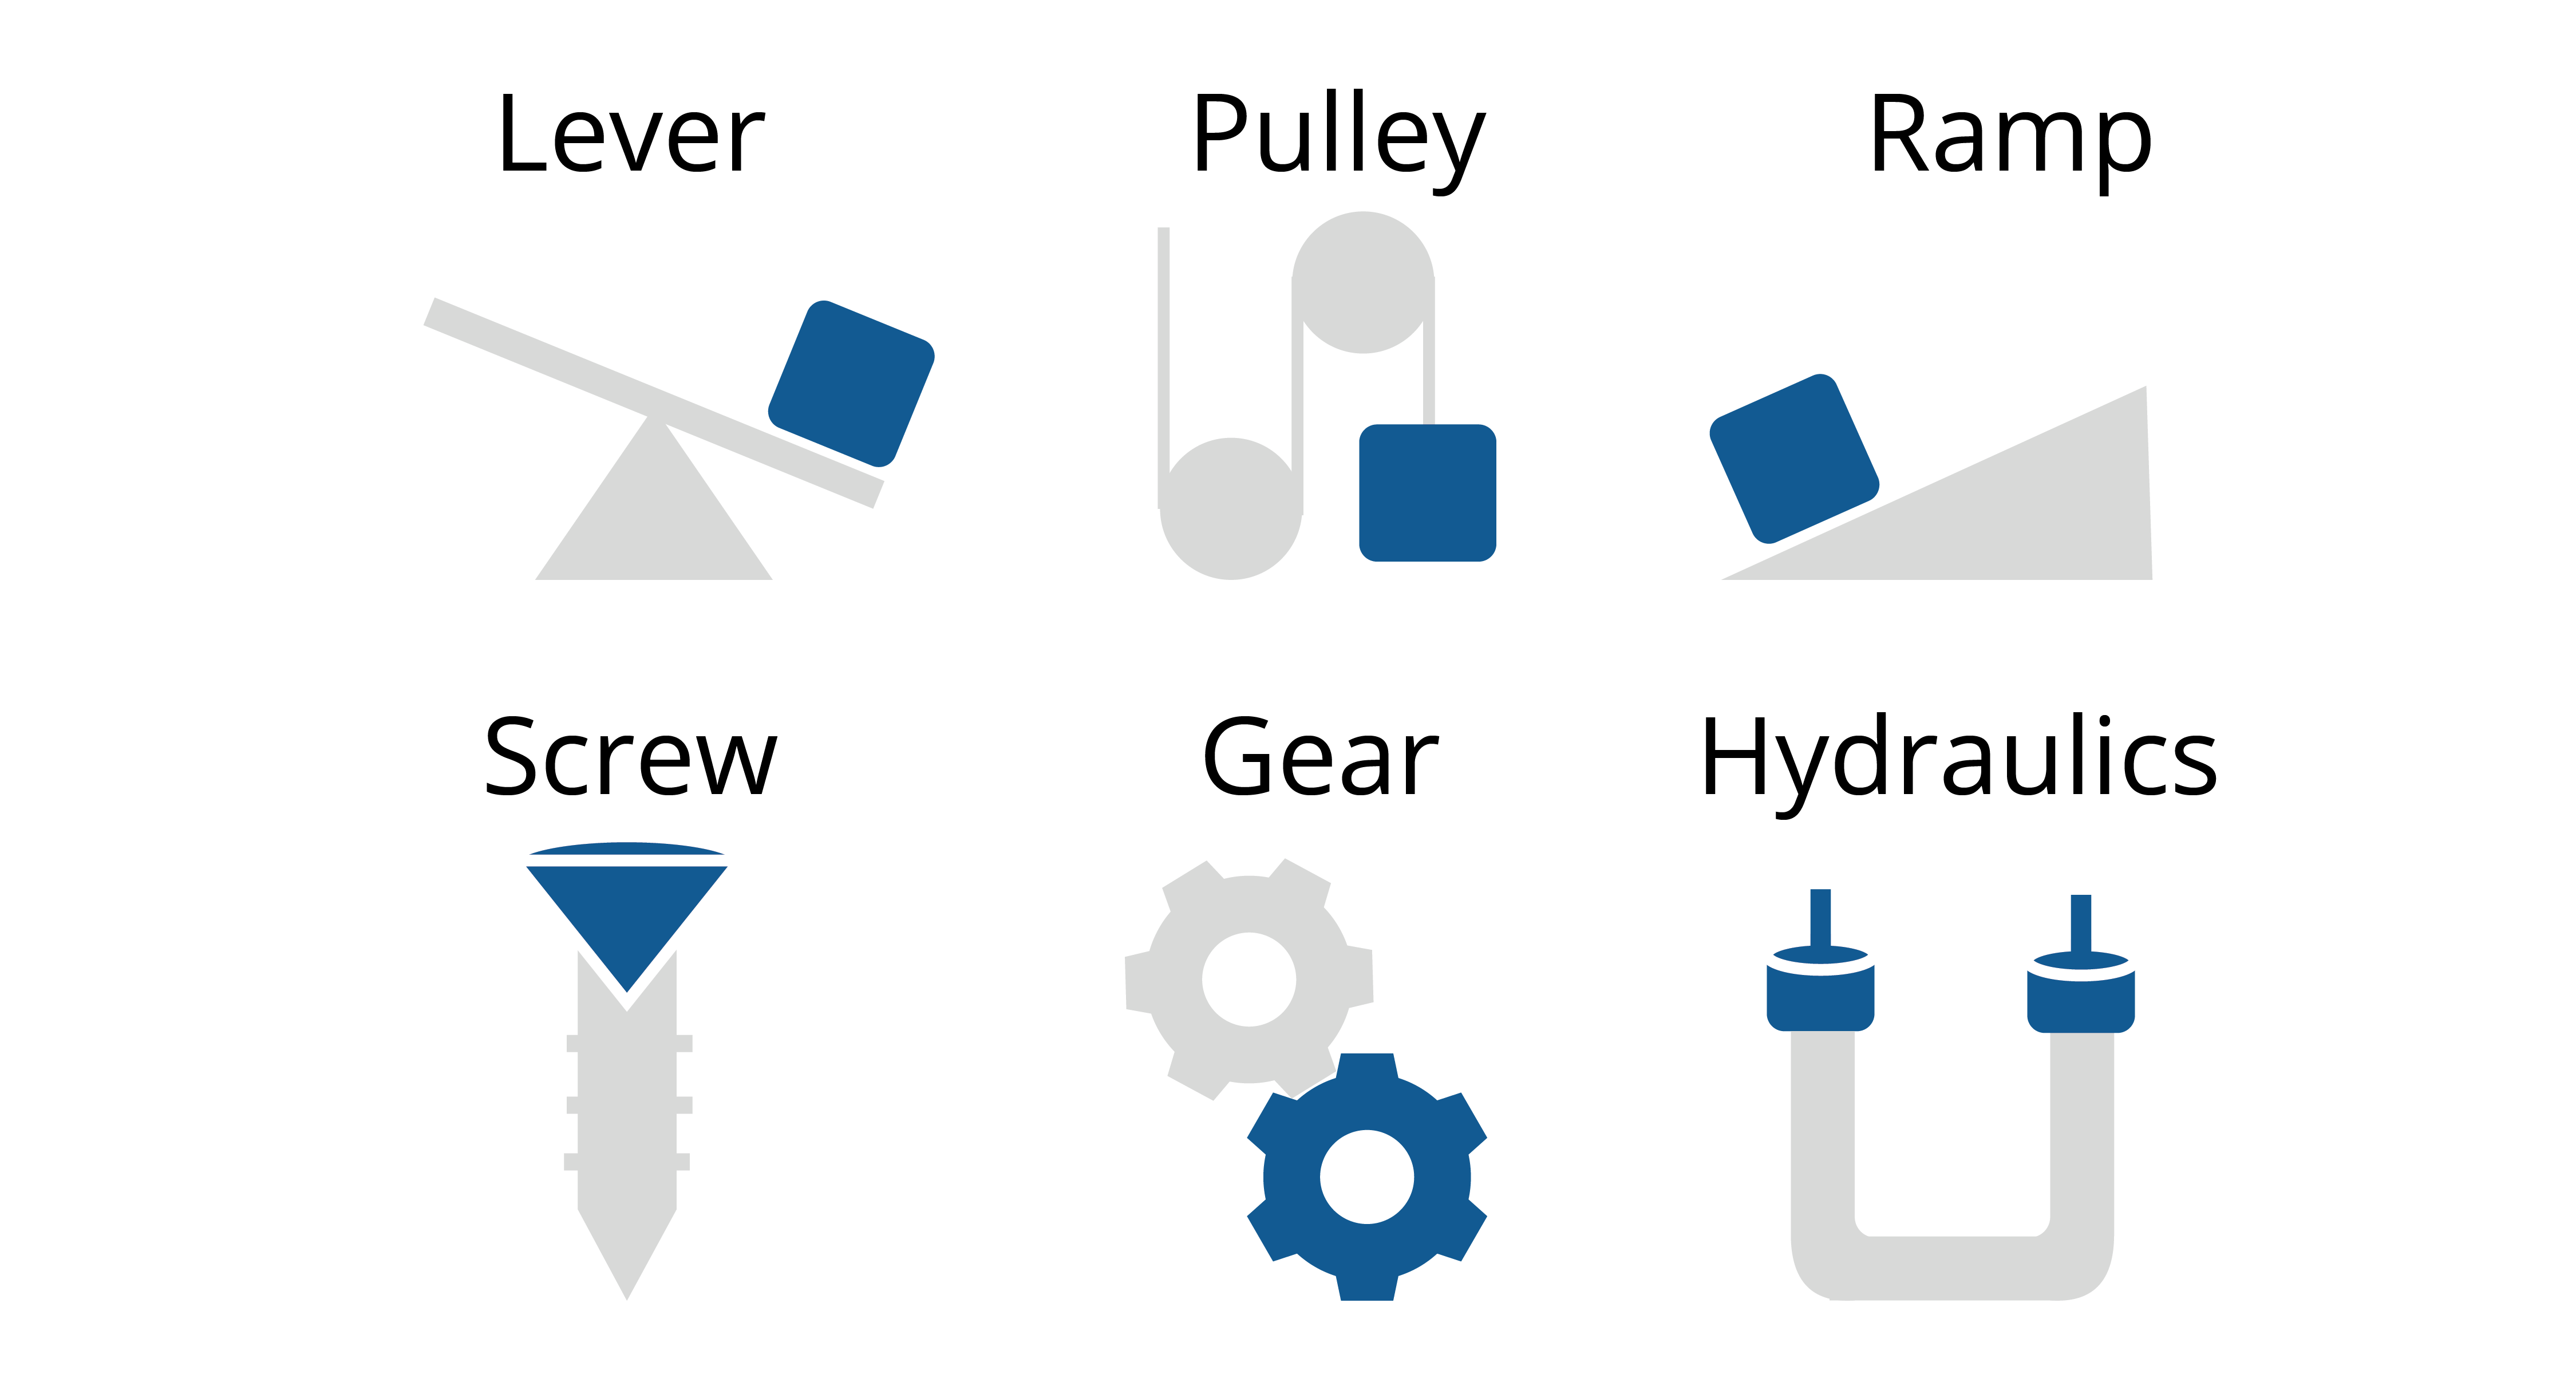
\includegraphics[width=\textwidth]{simplemachines.png}

While these machines can reduce the force needed, they do not change the total amount of work that must be done. For instance, if the force is reduced by a factor of three, the distance over which the force must be applied increases by the same factor.

The term \textit{mechanical advantage} refers to the increase in force achieved by using these machines.

\section{Levers}

A lever pivots on a fulcrum. To decrease the necessary force, the load is placed closer to the fulcrum than where the force is applied.

Physicists also discuss the concept of \newterm{torque} created by a force. When you apply force to a lever, the torque is the product of the force you exert and the distance from the point of rotation.

Torque is typically measured in newton-meters.

To balance two torques, the products of force and distance must be equal. Thus, assuming the forces are applied in the correct direction, the equation becomes:

\[
R_L F_L = R_A F_A
\]

where \( R_L \) and \( R_A \) represent the distances from the fulcrum to where the load’s force and the applied force are exerted, respectively, and \( F_L \) and \( F_A \) are the magnitudes of the forces.

\begin{Exercise}[title={Lever}, label=lever]
Paul, who weighs 70 kilograms, sits on a see-saw 4 meters from the fulcrum. Jan, who weighs 50 kilograms, wishes to balance the see-saw. How far should Jan sit from the fulcrum?
\end{Exercise}
\begin{Answer}[ref=lever]
Paul exerts a force of \( 70 \times 9.8 = 686 \) newtons at a distance of 4 meters from the fulcrum, creating a torque of \( 686 \times 4 = 2744 \) newton-meters. Jan exerts a force of \( 50 \times 9.8 = 490 \) newtons.

Let \( r \) be the distance from the fulcrum to Jan's seat. To balance the torques:

\[
490 \times r = 2744
\]

Solving for \( r \), we find \( r = \frac{2744}{490} \approx 5.6 \) meters.
\end{Answer}

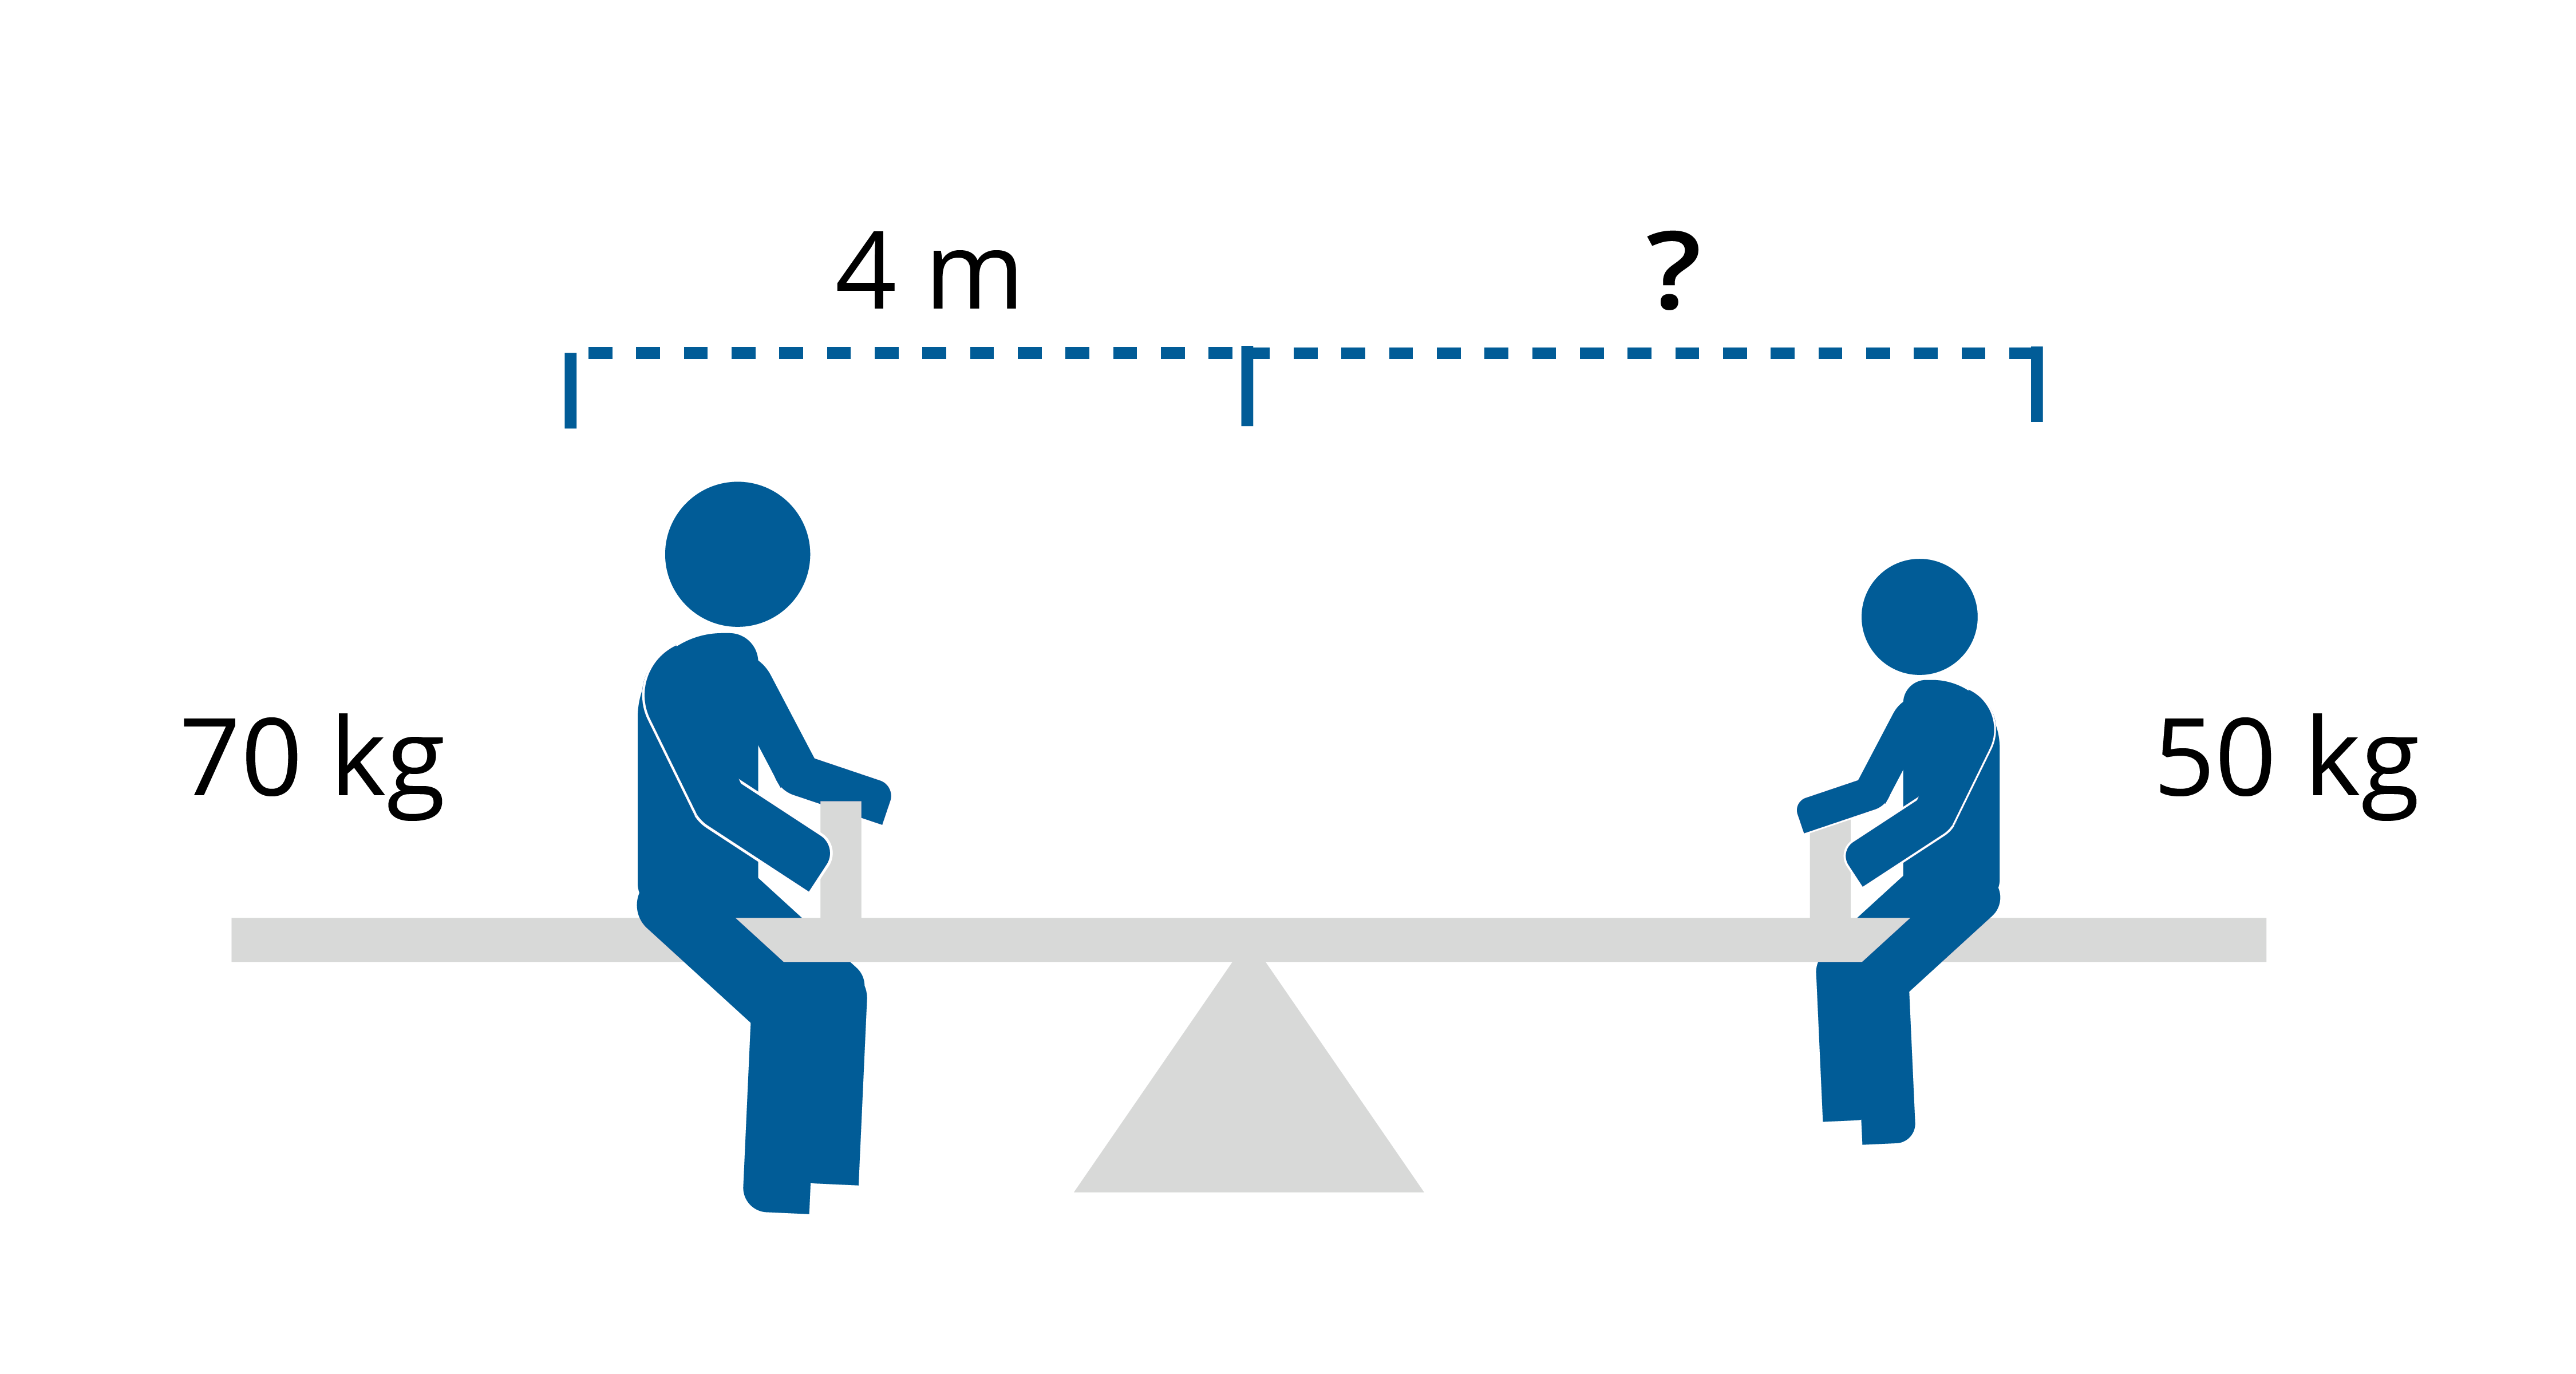
\includegraphics[width=0.6\textwidth]{seesaw.png}

\section{Inclined Planes}

Inclined planes, or ramps, allow you to roll or slide objects to a higher level. Steeper ramps require less mechanical advantage. For instance, it is much easier to roll a ball up a wheelchair ramp than a skateboard ramp.

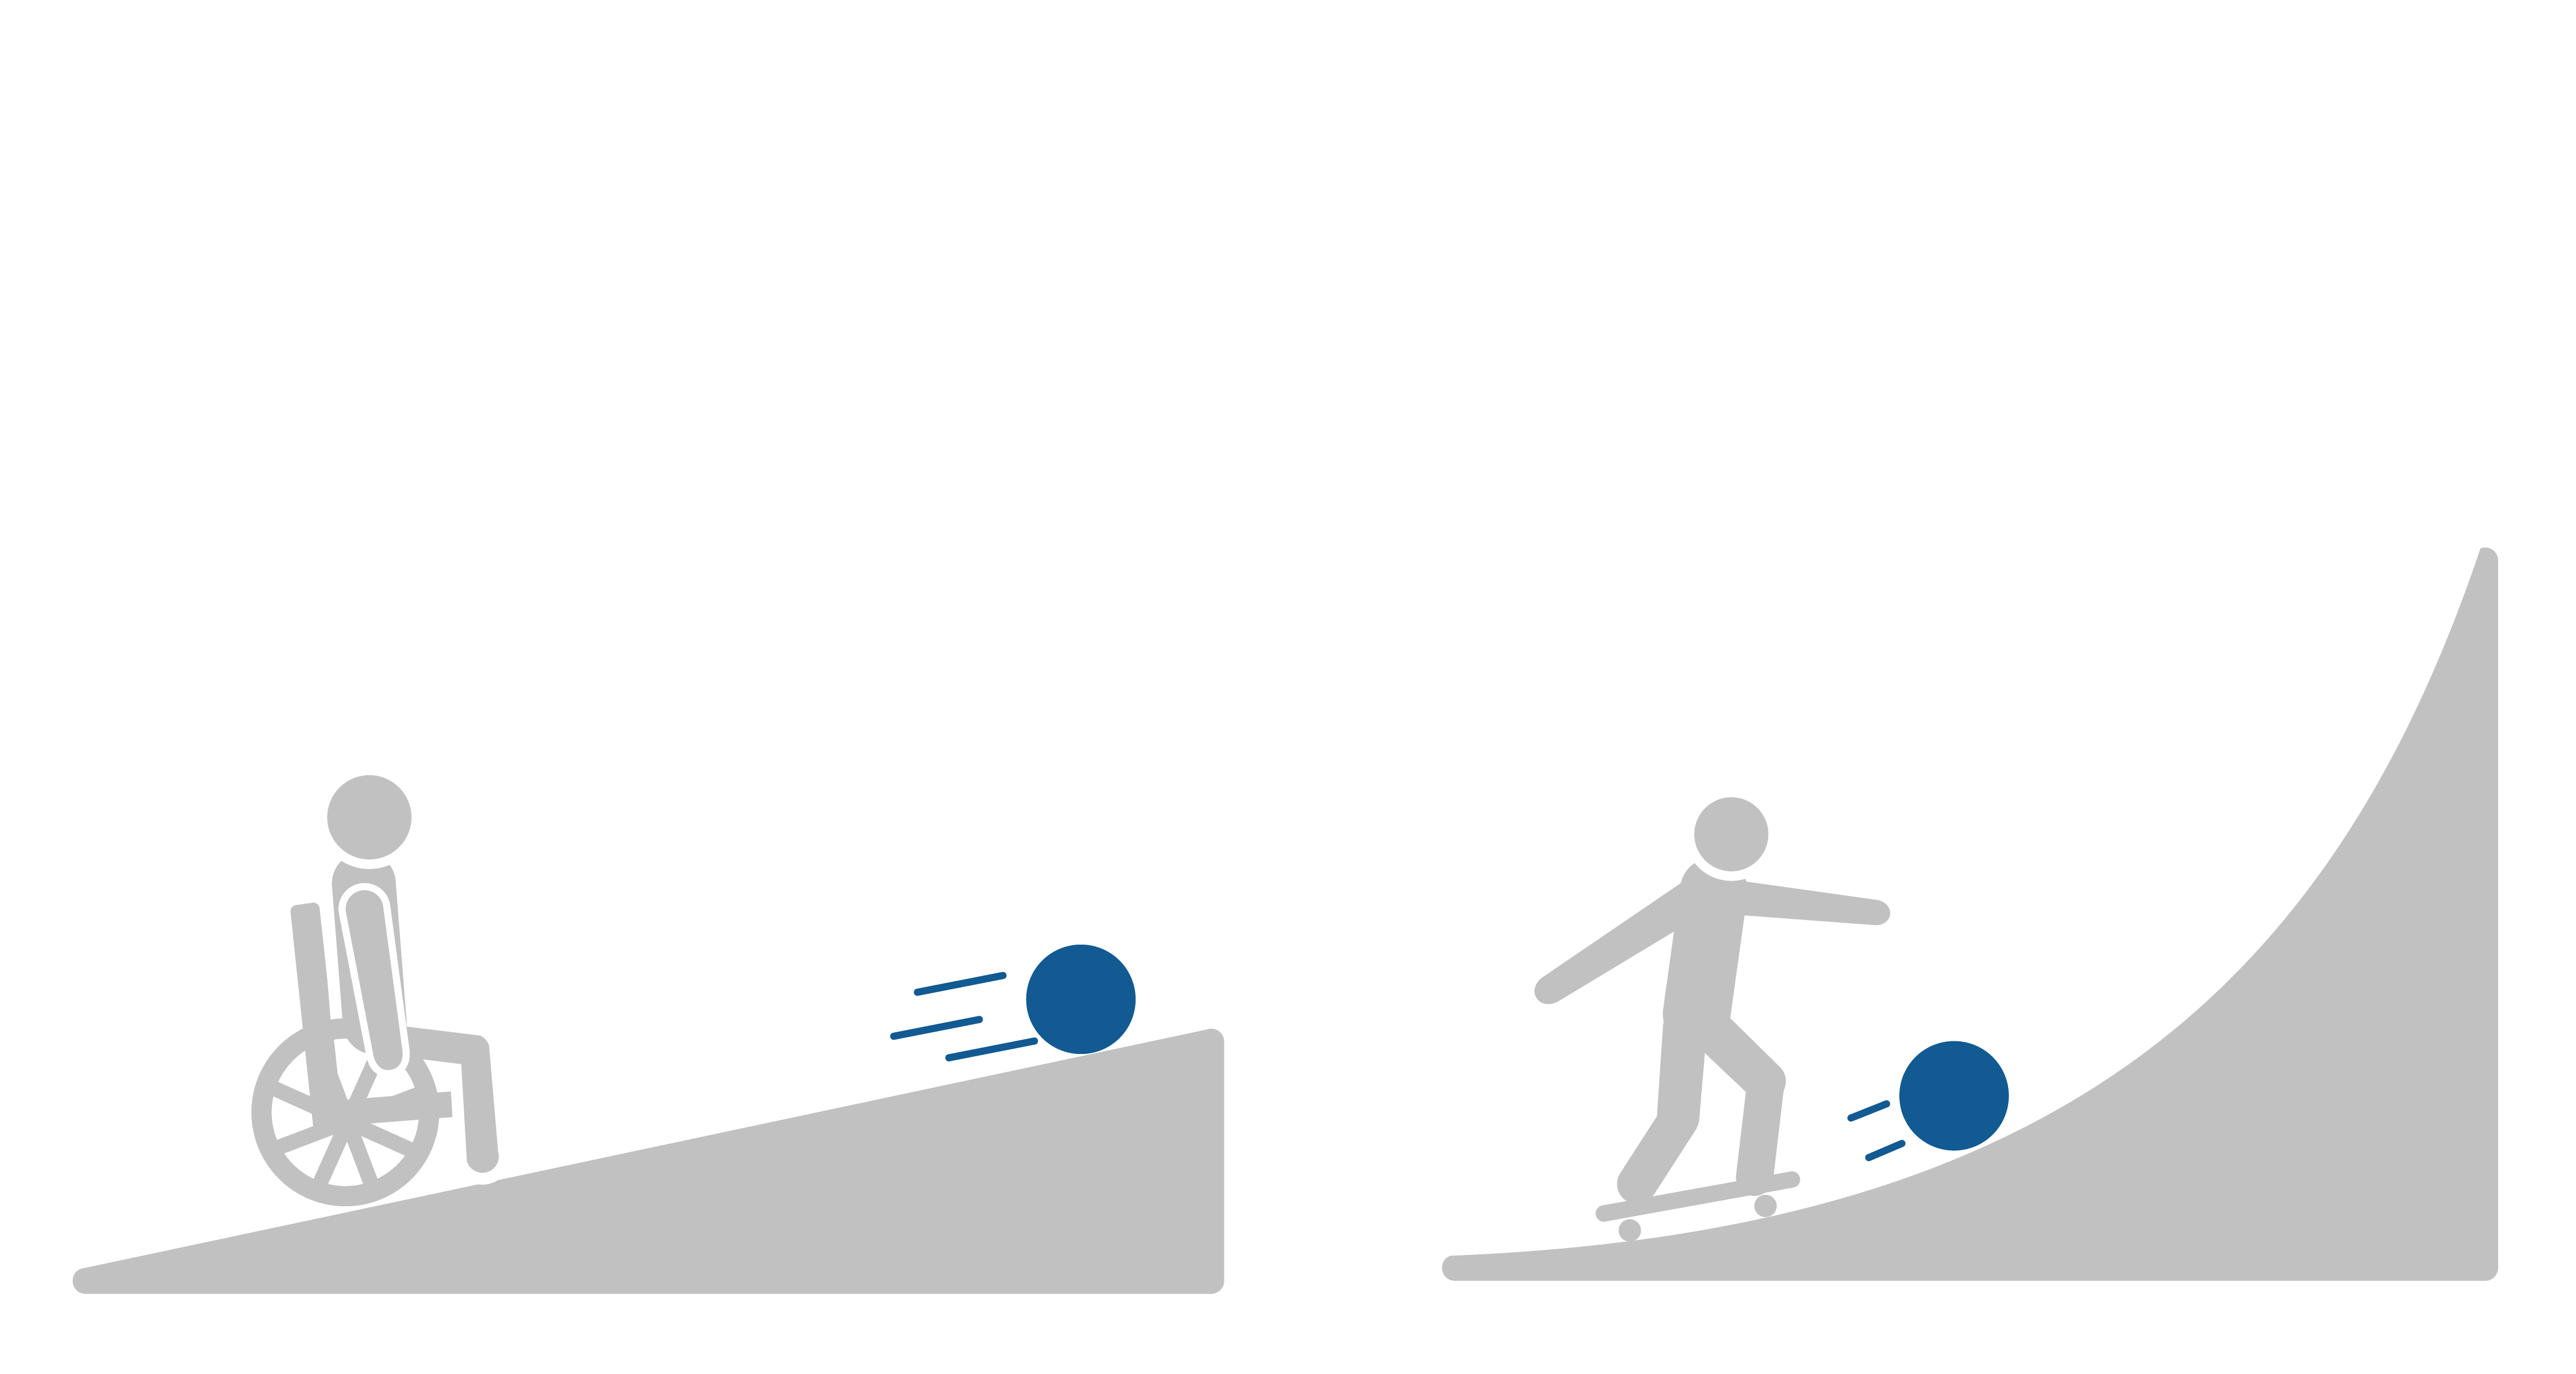
\includegraphics[width=\textwidth]{rampcomparison.png}

Assuming the incline has a constant steepness, the mechanical advantage is equal to the ratio of the length of the inclined plane to the height it rises.

If friction is neglected, the force required to push a weight up the inclined plane is given by:

\[
F_A = \frac{V}{L} F_G
\]

where \( F_A \) is the applied force, \( L \) is the length of the inclined plane, \( V \) is the vertical rise, and \( F_G \) is the gravitational force acting on the mass.

(We will discuss sine function later, but in case you're familiar with it, note that:

\[
\frac{V}{L} = \sin{\theta}
\]

where \( \theta \) is the angle between the inclined plane and the horizontal surface.)

\begin{Exercise}[title={Ramp}, label=ramp]
A barrel of oil weighs 136 kilograms. You can apply a force of up to 300 newtons. You need to get the barrel onto a platform that is 2 meters high. What is the shortest length of inclined plane you can use?
\end{Exercise}
\begin{Answer}[ref=ramp]
The weight of the barrel is \( 136 \times 9.8 = 1332.8 \) newtons.

Let \( L \) be the length of the inclined plane. The force needed to push the barrel up is related by:

\[
300 = \frac{2}{L} \times 1332.8
\]

Solving for \( L \), we find \( L = \frac{2 \times 1332.8}{300} \approx 8.885 \) meters.
\end{Answer}

\section{Gears}

Gears have teeth that mesh with each other. When you apply torque to one gear, it transfers torque to the other. The resulting torque is increased or decreased depending on the ratio of the number of teeth on the gears.

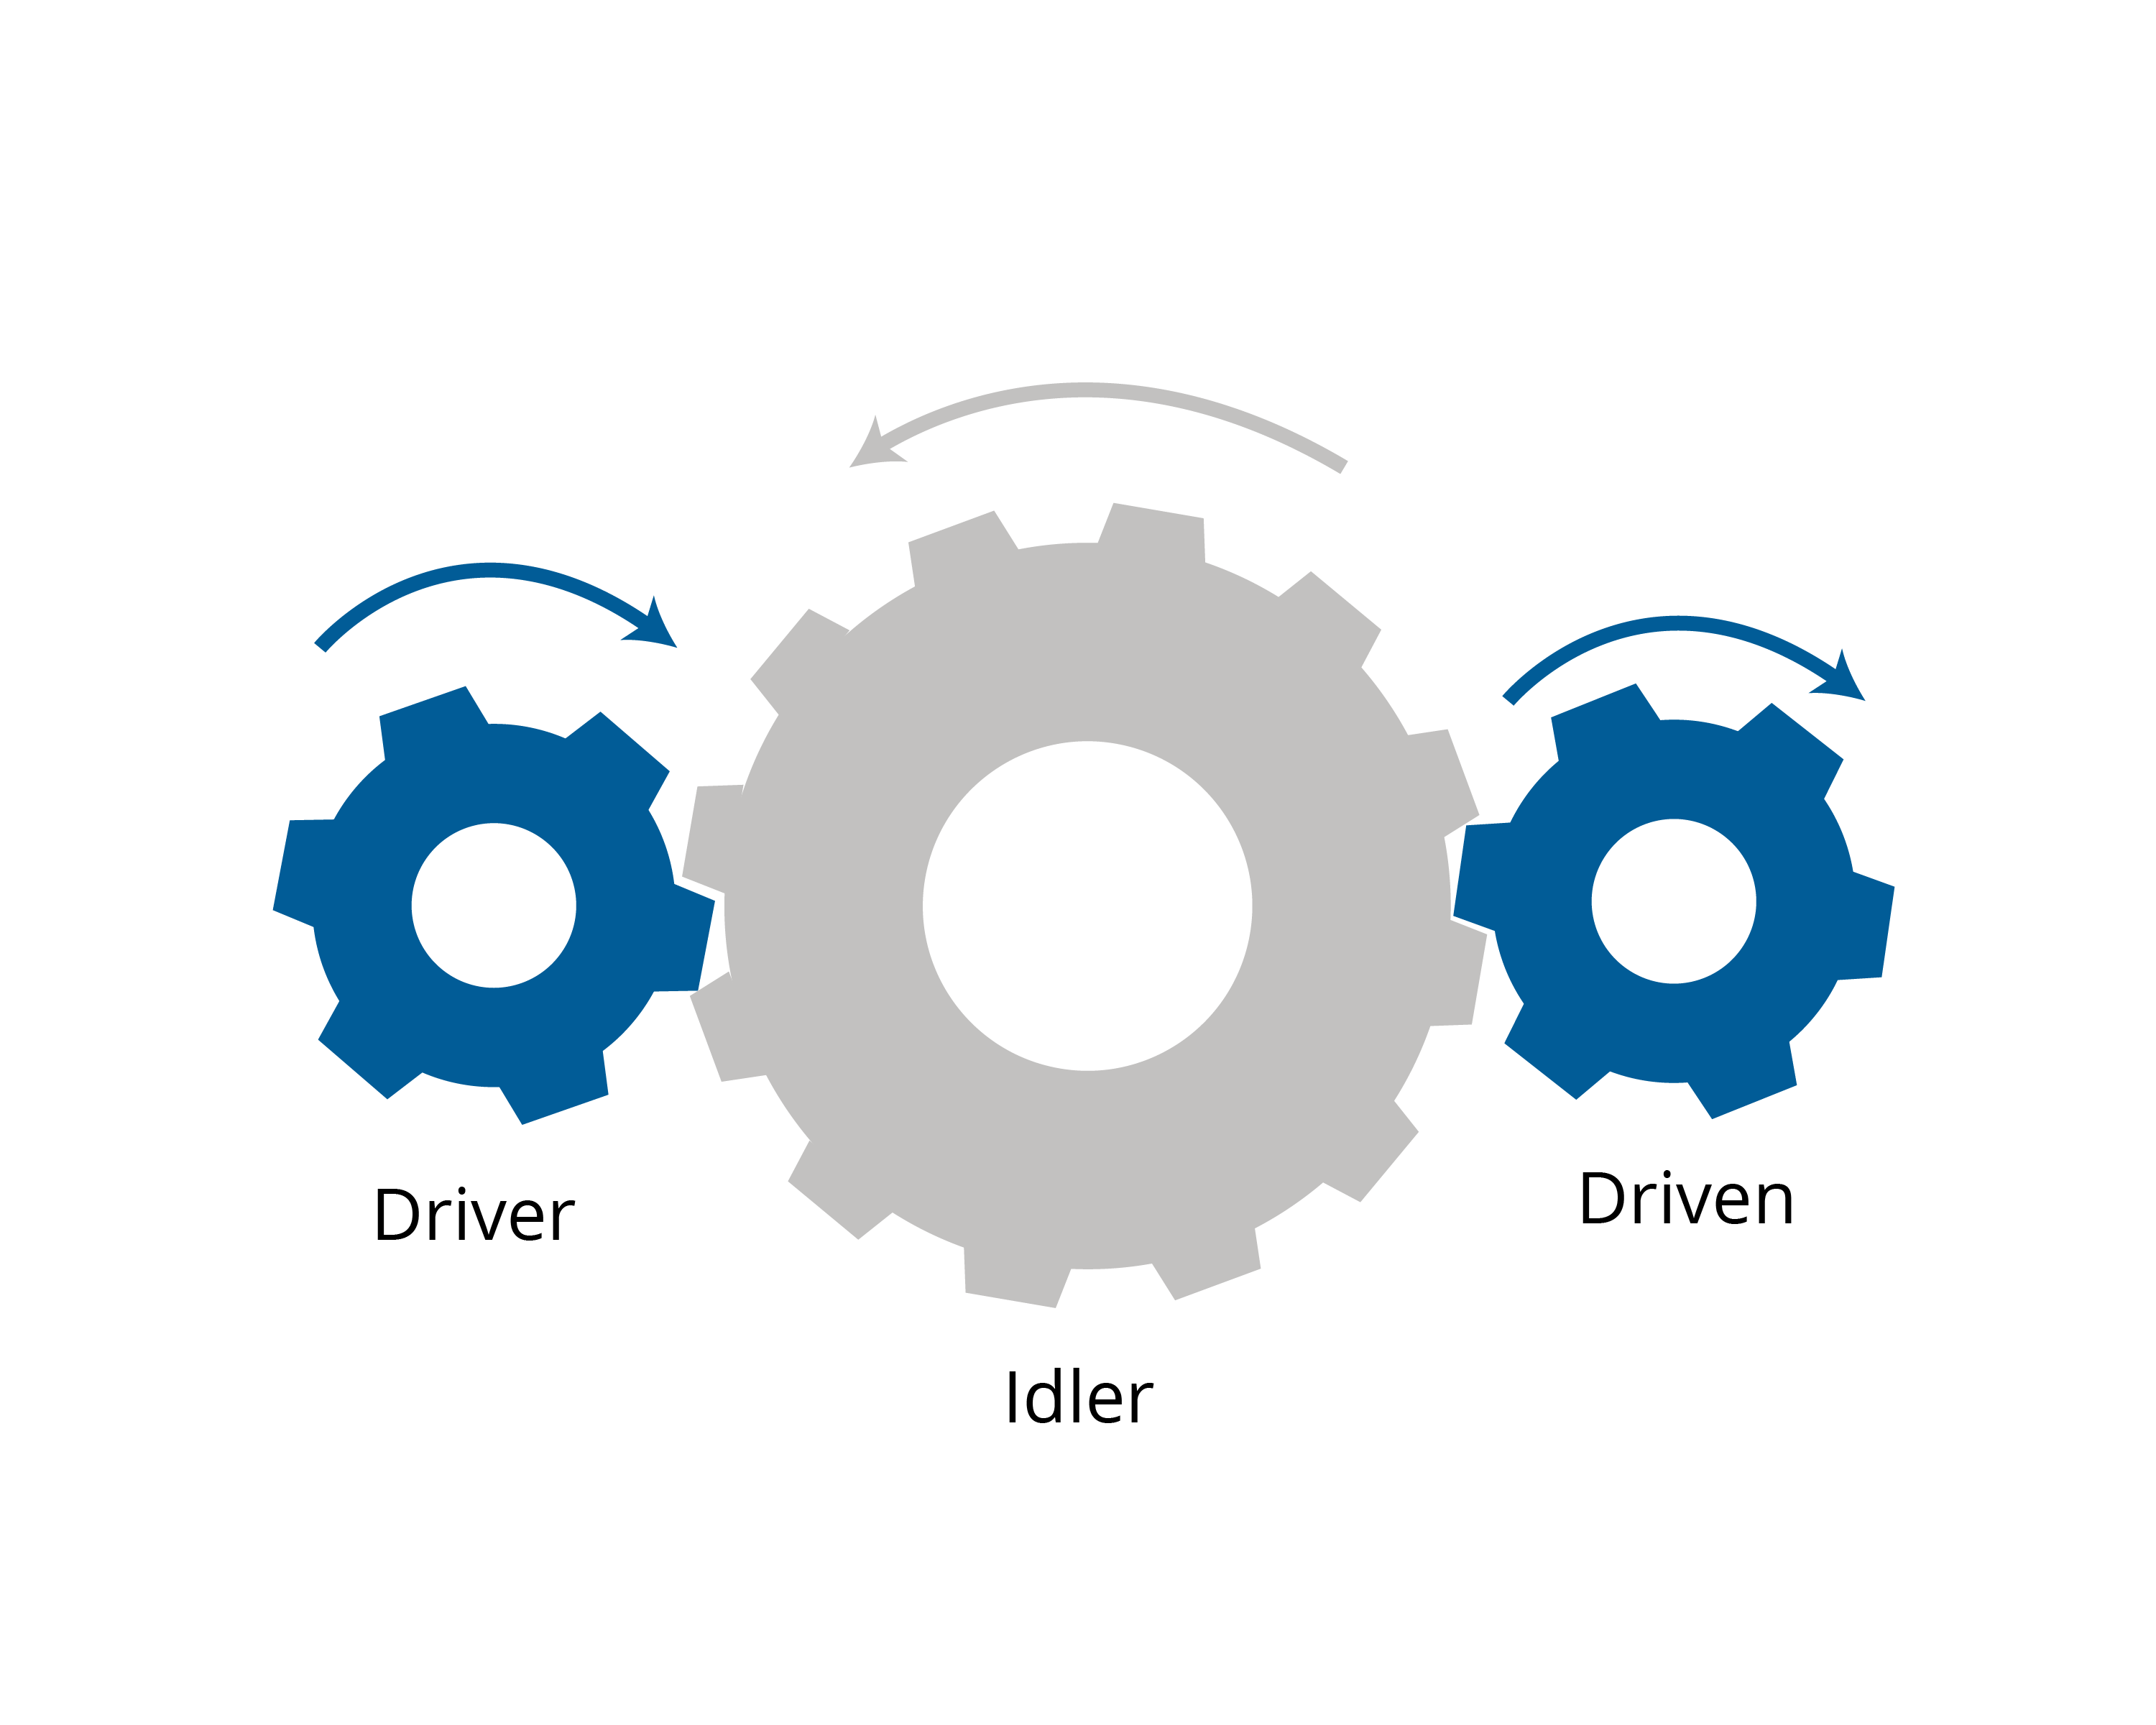
\includegraphics[width=0.7\textwidth]{gearsNew.png}

If \( N_A \) is the number of teeth on the gear you are turning with a torque of \( T_A \), and \( N_L \) is the number of teeth on the gear it is turning, the resulting torque is:

\[
T_L = \frac{N_A}{N_L} T_A
\]

\begin{Exercise}[title={Gears}, label=gear]
In a bicycle, the goal is not always to gain mechanical advantage, but to spin the pedals slower while applying more force.

You like to pedal your bike at 70 revolutions per minute. The chainring connected to your pedals has 53 teeth. The circumference of your tire is 2.2 meters. You want to ride at 583 meters per minute.

How many teeth should the rear sprocket have?
\end{Exercise}
\begin{Answer}[ref=gear]
The equation relating these quantities is:

\[
583 = 70 \times 2.2 \times \frac{53}{n}
\]

Solving for \( n \), we find \( n = 14 \) teeth.
\end{Answer}

\section{Hydraulics}

In a hydraulic system, such as a car's braking system, you exert force on a piston filled with fluid. The fluid transmits this pressure into another cylinder, where it pushes yet another piston that moves the load.

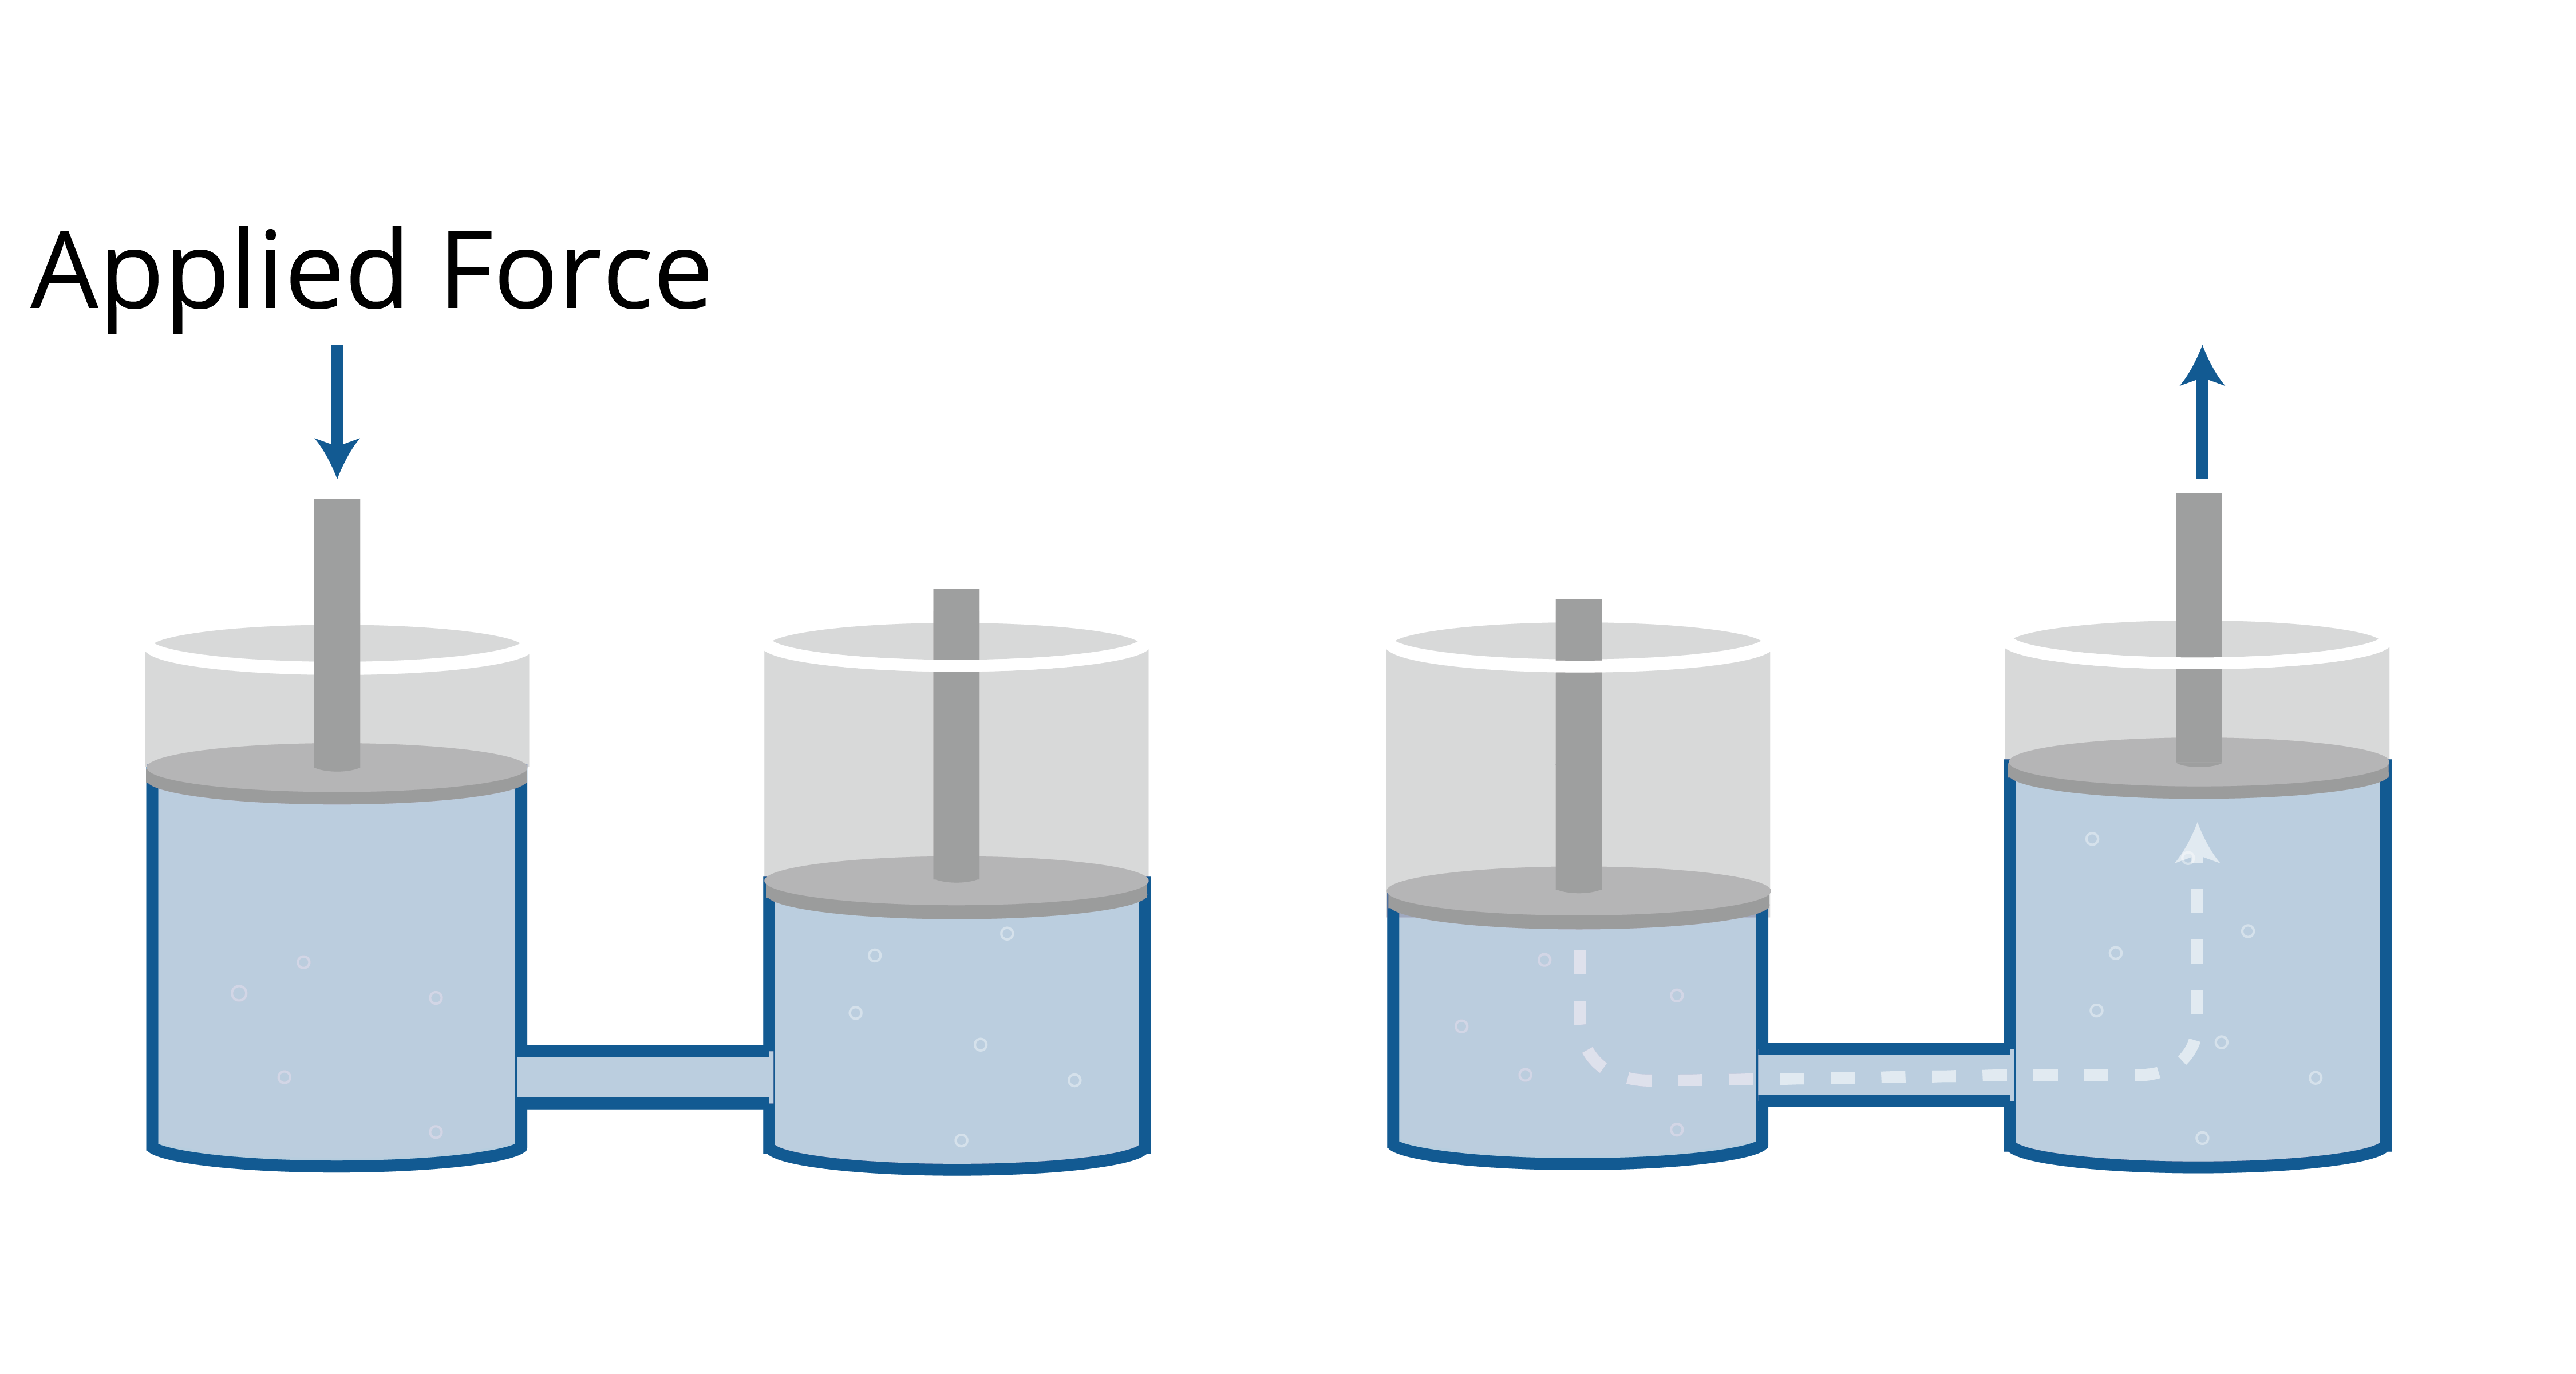
\includegraphics[width=\textwidth]{hydraulicsNew.png}

The pressure in the fluid is typically measured in pascals (Pa), which is equivalent to \(N / m^2\). We will use pascals for this calculation.

To calculate the pressure you create, divide the force applied by the area of the piston head. To determine the force on the other piston, multiply the pressure by the area of the second piston.

\begin{Exercise}[title={Hydraulics}, label=hydraulics]
Your car has disc brakes. When you apply 2,500,000 pascals of pressure to the brake fluid, the car stops quickly. As the car designer, you want this to require only 12 newtons of force from the driver's foot.

What should the radius of the master cylinder (the piston the driver pushes) be?
\end{Exercise}
\begin{Answer}[ref=hydraulics]
We are solving for the radius \( r \) of the piston. The area of the piston is \( \pi r^2 \), so the pressure is:

\[
\text{Pressure} = \frac{12}{\pi r^2}
\]

Setting the pressure equal to 2,500,000 pascals:

\[
2,500,000 = \frac{12}{\pi r^2}
\]

Solving for \( r \), we find:

\[
r = \sqrt{\frac{12}{\pi \times 2.5 \times 10^6}} \approx 0.00124 \text{ meters}.
\]
\end{Answer}

\graphicspath{{../../Chapters/biases1/en_US}}
\chapter{Cognitivie Biases 1}


Our brains were designed over millions of years by the evolutionary
process. The resulting mind is an amazing and powerful tool, but it is
not flawless. The human brain has tendencies (or biases) that nudge us
toward bad judgment and poor decisions.

It would be irresponsible for us to teach you powerful ideas without
also teaching you about these cognitive biases. There are about 50
that you should know about, so we will have a few that introduce them.

\section{Fundamental Attribution Error}

You tend to attribute
the mistakes of another person to their character, but attribute your
own mistakes to the situation.

Let's say you are at lunch and someone asks you ``Why was Larry late
for class ?''  You are likely to say ``Larry is lazy
and disorganized.''

If someone asks you ``Why were you late for class last week?''  You
are likely to say, ``I don't remember; The class before it must have
run long.''

The solution? Cut people some slack. You probably don't know the whole
story, so assume that their character is as strong as yours.

Or maybe you also need to hold yourself to a higher standard? Do you find
yourself frequently rationalizing your bad judgment, lateness, or
rudeness?  This could be an opportunity for you to become a better
person whose character is stronger regardless of the situation.

\section{Self-Serving Bias}

\newterm{Self-serving bias} is when you blame the situation for your
failures, but attribute your successes to your strengths.

For example, when asked ``Why did you lose the match?'' you are likely
to answer ``The referee wasn't fair.''  When you are asked ``Why did
you win the match?'' you are likely to answer ``Because I have been
training for weeks, and I was very focused.''

This bias tends to make us feel better about ourselves, but it makes it
difficult for us to be objective about our strengths and weaknesses.

\section{In-group favoritism}

\newterm{In-group favoritism}: We tend to favor people who are in
a group with us over people who are not in groups with us.

When asked ``Who is the better goalie, Ted or John?''

If Ted is a Star Trek fan like you, you are likely to think he is also
a good goalie.

As you might imagine, this unconscious tendency is the source of a lot
of subtle discrimination based on race, gender, age, and religion.

\section{The Bandwagon Effect and Groupthink}

\newterm{The bandwagon effect} is our tendency to believe the same
things that the people around us believe. This is how fads spread so
quickly: one person buys in, and then the people they know have a
strong tencdency to buy in as well.

\newterm{Groupthink} is similar: To create harmony with the
people around us, we go along with things we disagree with.

It takes a lot of perspective to recognize when those around us are
wrong. And it takes even more courage to disagree with them.

\section{The Curse of Knowledge}

Once you know something, you tend to assume everyone else knows it too.

This is why teaching is sometimes difficult: a teacher will assume
that everyone in the audience already knows the same things the
teacher knows.

Also, when we learn that a friend doesn't know something that we know,
we are often very surprised.  This surprise can sometimes manifest as
hurtful behavior.

When I find a gap in a friend's knowledge, I try to remind myself that
the friend certainly knows many things that I don't.  I also try to
imagine how it would feel if they teased me for my ignorance.

\section{False Consensus}

You tend to believe that more people agree with us than is actually
the case. For example, if you are a member of a particular religion,
you tend to overestimate the percentage of people in the world who are
members of that religion.

When people vote in elections, they are often surprised when their
preferred candidate loses. ``Everyone, and I mean EVERYONE, voted for
Smith!'' they yell.  ``There must have been a mistake in counting the
votes.''

\section{The Spotlight Effect}

You tend to overestimate how much other people are paying attention to
your behavior and appearance.

Think of six people that you talked to today.  Can you even remember what
shoes most of them were wearing? Do you care? Do you think any of them
remember which shoes you wore today?

There is an old saying ``You would worry a lot less about how people
think of you if you realized how rarely they do.''

\section{The Dunning-Kruger Effect}

The less you know, the more confident you are.

When a person doesn't know all the nuance and context in which a question is
asked, the question seems simple. Thus the person tends to be confident in
their answer.  As they learn more about the complexity of the space in
which the question lives, they often realize the answer is not nearly so
obvious.

For example, a lot of people will confidently proclaim ``Taxes are too
high! We need to lower taxes.''  An economist who has studied
government budgets, deficits, history, and monetary policy, might say
something like ``Maybe taxes \emph{are} too high.  Or maybe they are
too low. Or maybe we are taxing the wrong things. It is a 
complex question.''

When I am talking with people about a particular topic, I do my best
to defer to the person in the conversation who I think has the most
knowledge in the area. If I disagree with the person, I try to figure
out why our opinions are different.

Similarly, you should assume that any opinion that is voiced in an
internet discussion is wildly over-simplified.  If you really care
about the subject, read a book by a respected expert. Yes, a whole
book -- there are few interesting topics that can be legitimately
explained in less than 100 pages.

\section{Confirmation Bias}

You tend to find and remember information that supports
beliefs you already have. You tend to avoid and dismiss information
that contradicts your beliefs.

If you believe that intelligent creatures have visited from other
planets, you will tend to look for data to support your beliefs. When
you find data that shows that it is just too far for any creature to
travel, you will try to find a reason why the data is incorrect.

Confirmation bias is one reason why people don't change their beliefs
more often.

Confirmation bias wrecks many, many studies. The person doing the
study often has a hypothesis that they believe and very much want to
prove true. It is very tempting to discard data that doesn't support
the hypothesis. Or maybe the person throws all the data away and experiments again and again until they get the result they want.

When you design an experiment, you must describe it explicitly before
you start. You must tell someone: ``If the hypothesis I love is
incorrect, the results will look like this.  If the hypothesis I love
is correct, the results will look like that. And if the results look
any other way, I have neither proved nor disproved the hypothesis.''

Once the experiment is underway, you must not change the plan and you
must not discard any data.

This is scientific integrity. You should demand it from yourself, and
you should expect it from others.

\section{Survivorship bias}

You will pay more attention to those that survived a process than
those who failed.

After looking at a lot of old houses, you might say ``In the 1880s,
they built great houses.'' However, you haven't seen the houses that
were built in the 1880s and didn't survive.  Which houses tended to
survive for a long time? Only the great houses -- you are
basing your opinion on a very skewed sample.


\graphicspath{{../../Chapters/buoyancy/en_US}}
\chapter{Buoyancy}

The word buoyancy probably brings to mind images of floating in water. Before we dive in, let's zoom out for a better understanding of everything buoyancy entails. You may be thinking: I want to be a computer programmer, why do I need to know about buoyancy? You might be surprised! This topic is much bigger than it seems at first glance. 

Buoyancy concerns the ways in which liquids and gasses interact with gravity. The concept of buoyancy is connected to fundamental concepts about how the universe works. The \newterm{buoyant force}, as it is known in engineering, is an important concept that has wide ranging applications. A big part of engineering is moving stuff around, and understanding buoyancy helps us solve problems where we need to move things in and through fluids. Even if you don't have plans to build a robotic submarine, these are incredibly useful ideas to be familiar with. We will start exploring the topic with familiar scenarios around boats and water.

When you put a boat into water, it will sink into the water until
the mass of the water it displaces is equal to the mass of the
boat. We think of this in terms of forces. Gravity pulls the mass of
the boat down; the \newterm{buoyant force} pushes the boat up. A boat
dropped into the water will bob up and down at first before reaching an
\newterm{equilibrium} where the two forces are equal.
% FIXME: Define displacement, and velocity. It is not defined in workbook one or this chapter (I think that would help) - Arjan
% ADD: Explain Action Reaction Pairs in previous chapter
% ADD: Archimedes principle

The buoyant force pushes things up, fighting against the force of
gravity. The force is equal to the weight of the fluid being
replaced. For example, a cubic meter of freshwater has a mass of
about 1000kg. If you submerge anything with a volume of one meter in
freshwater on earth, the buoyant force will be about 9800 newtons ($\text{mass} \times \ \text{gravity})$.

For some things, like a block of styrofoam, this buoyant force will be
sufficient to carry it to the surface. Once it reaches the surface, it
will continue to rise (displacing less water) until the mass of the
water it displaces is equal to its mass. And then we say ``It floats!''

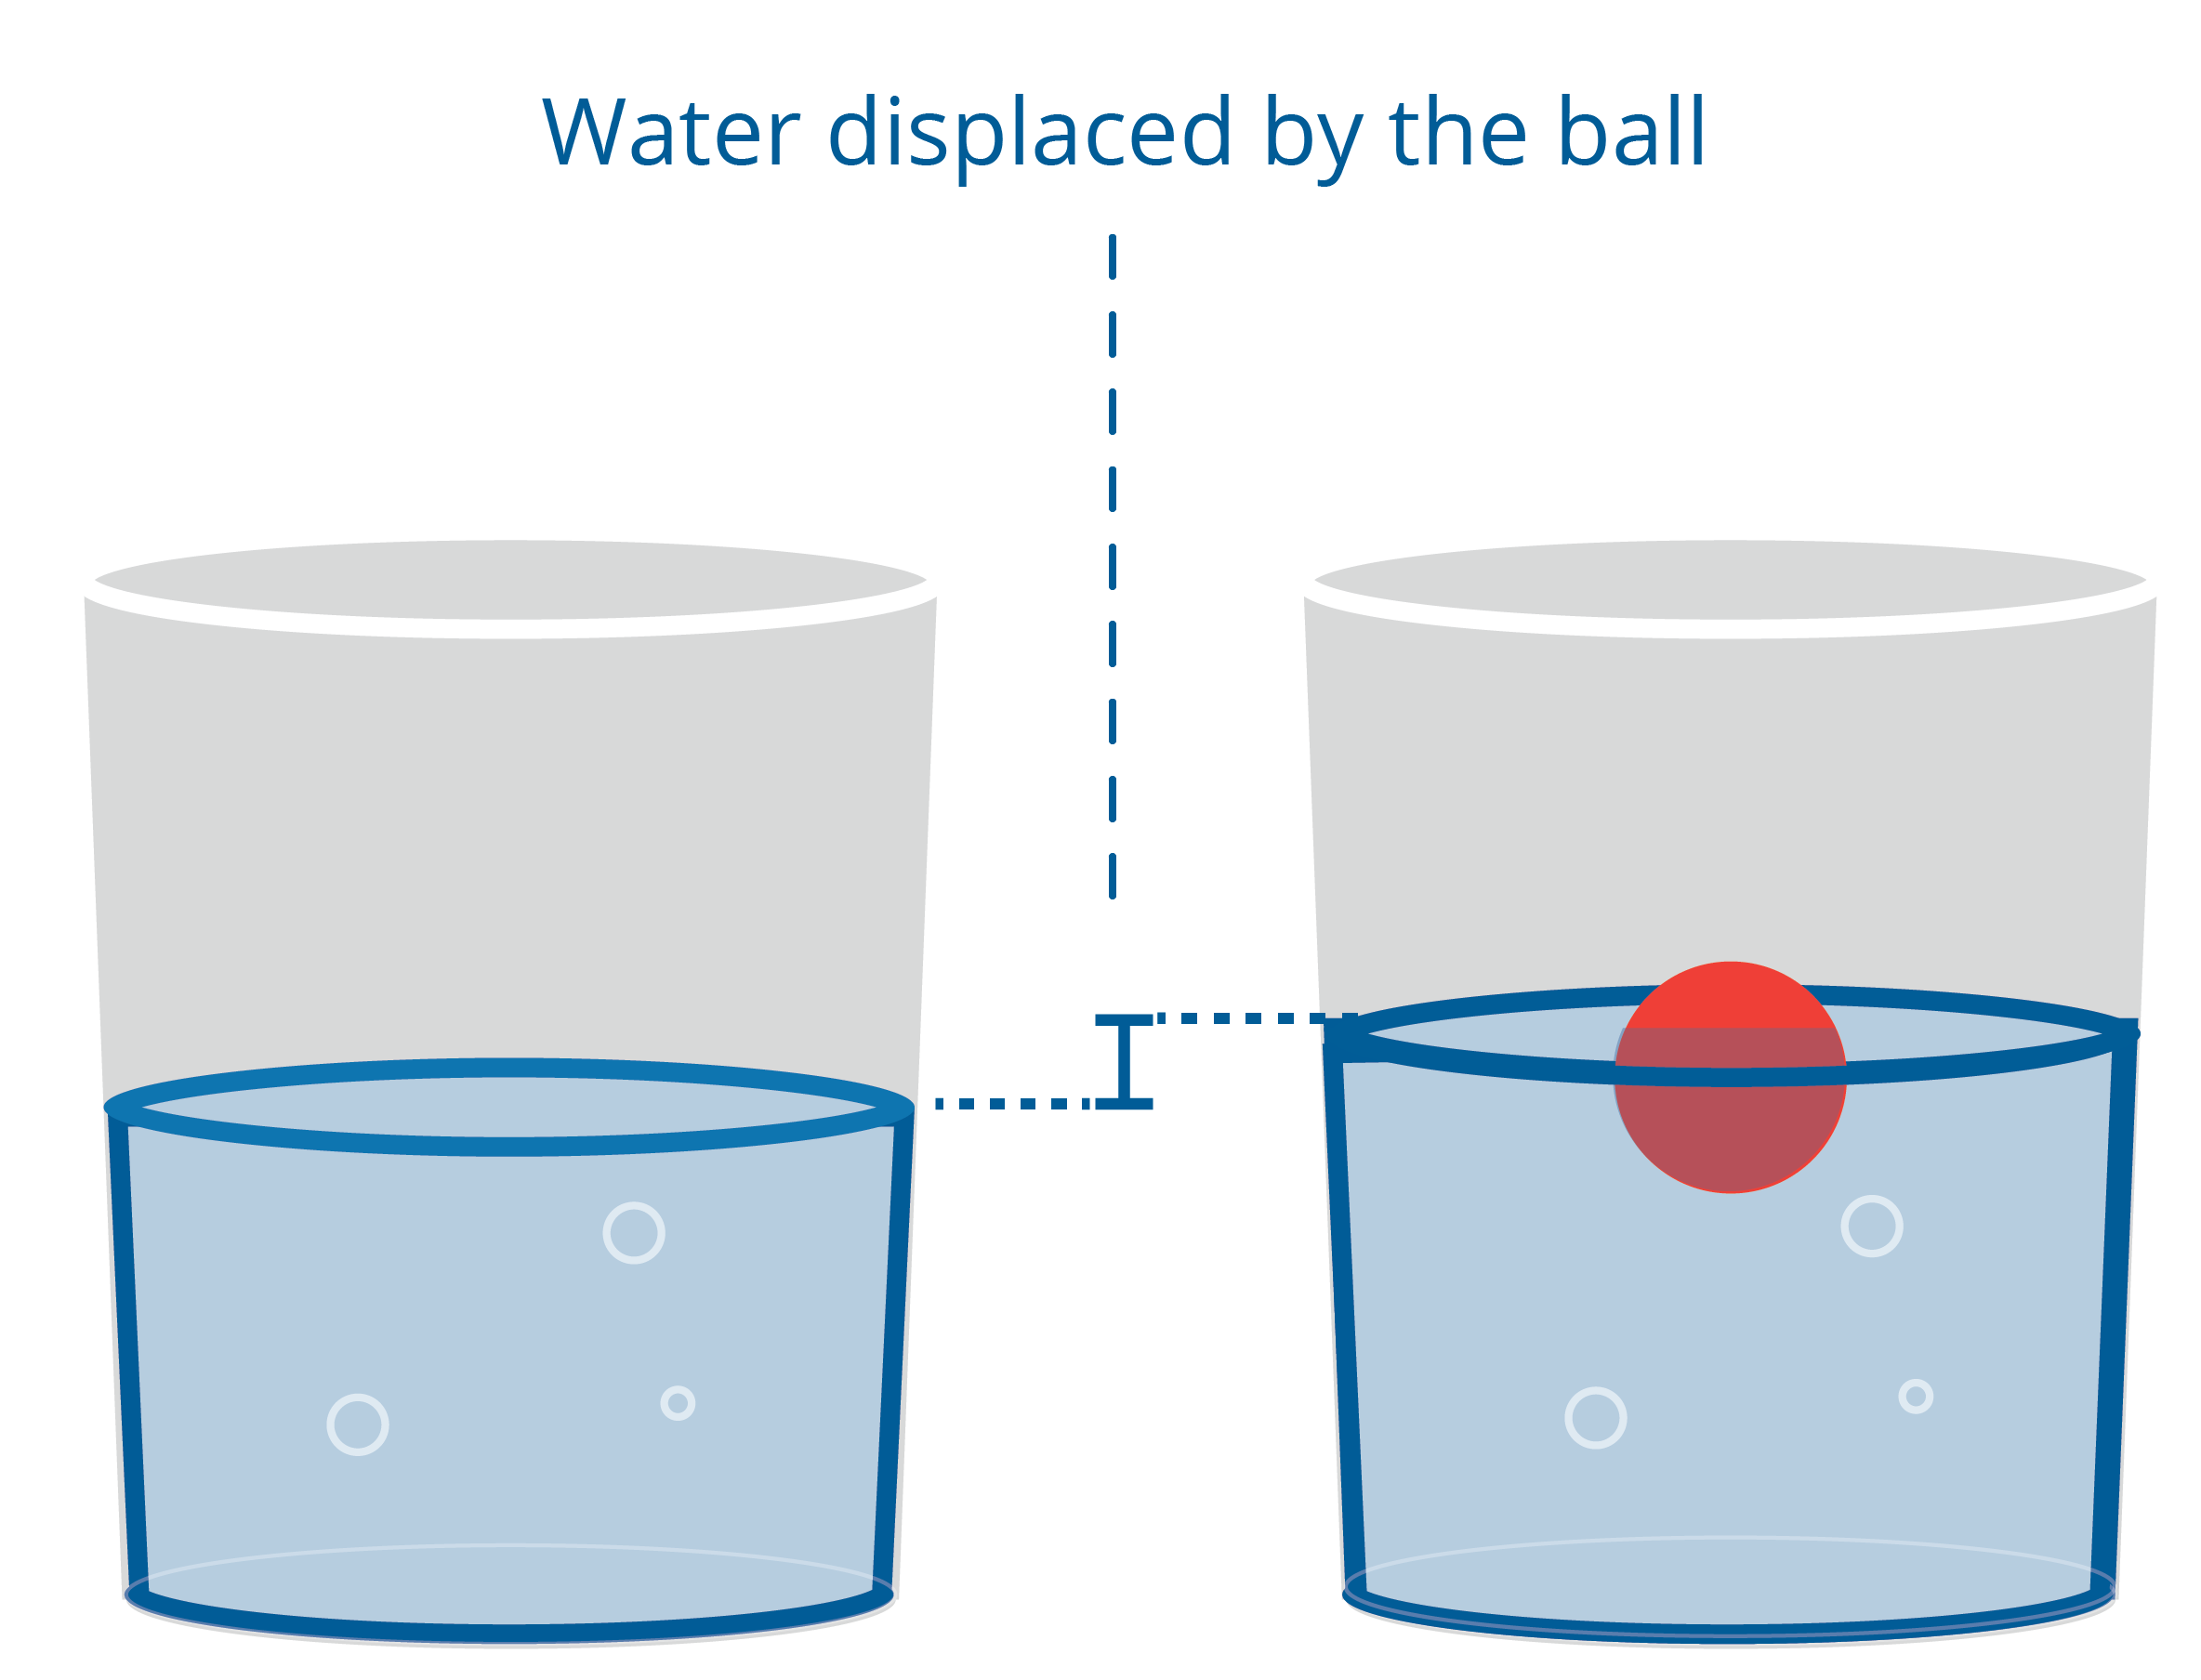
\includegraphics[width=.6\textwidth]{waterDisplacement.png}

For some things, like a block of lead, the buoyant force is not
 sufficient to lift it to the surface, and then we say ``It sinks!''

This is why a helium balloon floats through the air. The air
that it displaces weighs more than the balloon and the helium itself. (It is easy to forget that air has a mass, but it does.)

\begin{Exercise}[title={Buoyancy}, label=buoyancy]
  You have an aluminum box that has a heavy base, so it will always
  float upright. The box and its contents weigh 10 kg. Its base is 0.3 m x 0.4 m. It is 1m tall.

  When you drop it into freshwater ($1000 kg/m^3$), how far will it sink
  before it reaches equilibrium?\index{equilibrium}

\end{Exercise}
\begin{Answer}[ref=buoyancy]
  Equilibrium will be achieved when the box has displaced 10 kg of water. In other words, when it has displaced $0.01$ cubic meters.

  The area of the base of the box is 0.12 square meters. So if the
  box sinks $x$ meters into the water it will displace $0.12 x$ cubic
  meters.

  Thus at equilibrium $x = \frac{0.01}{0.12} \approx 0.083$ m. So
  the box will sink 8.3 cm into the water before reaching equilibrium.
\end{Answer}

\section{The Mechanism of Buoyancy: Pressure}

As you dive down in the ocean, you will experience greater and
greater pressure from the water. And if you take a balloon with you, you
will gradually see it get smaller as the water pressure compresses the
air in the balloon.

Let's say you are 3 meters below the surface of the water. What is the
pressure in Pascals (newtons per square meter)? You can think of the
water as a column of water crushing down upon you. The pressure over
a square meter is the weight of 3 cubic meters of water pressing down.

$$p = (3)(1000)(9.8) = 29,400 \text{ Pa }$$

This is called \newterm{hydrostatic pressure}. The general rule for
hydrostatic pressure in Pascals $p$ is

$p = d g h$

where $d$ is the density of the fluid
in kg per cubic meter, $g$ is the acceleration due to gravity in
$m/s^2$, and $h$ is the height of the column of fluid above you.

So where does buoyant force come from? Basically, the pressure pushing up on the
deepest part of the object is higher than the pressure pushing down on
the shallowest part of the object. That is where bouyancy comes from.

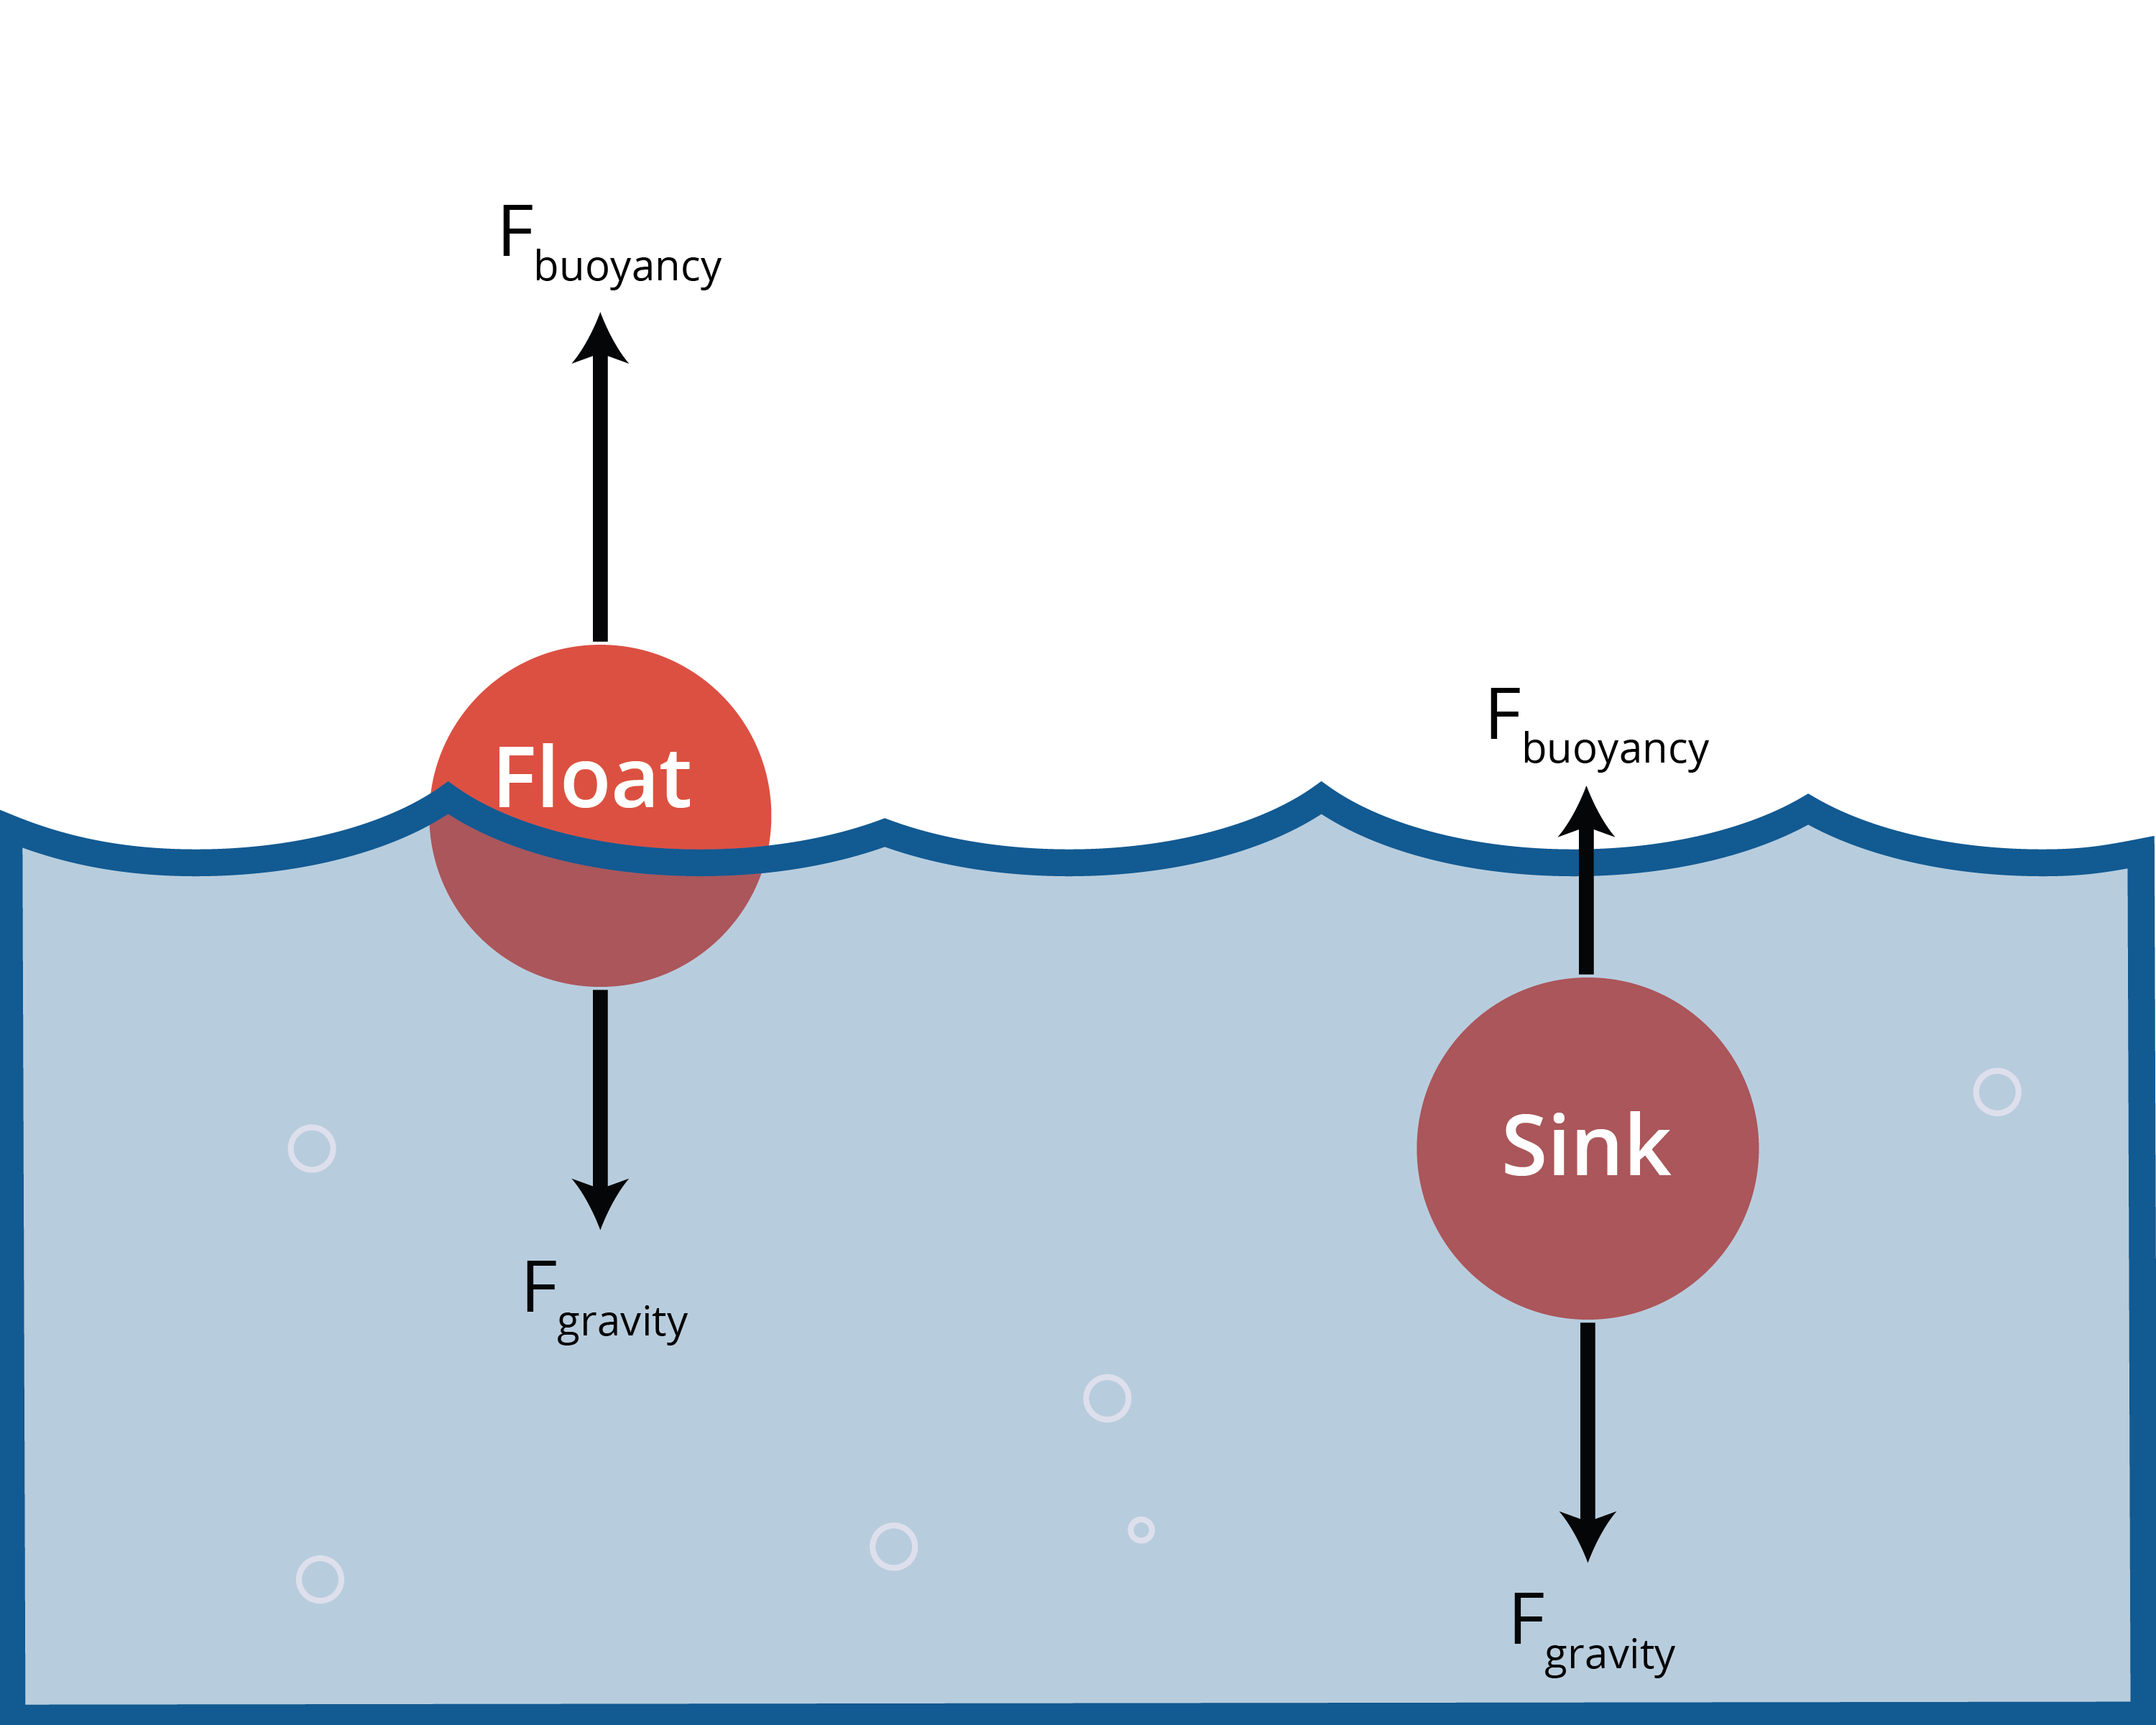
\includegraphics[width=.6\textwidth]{buoyancy.png}

\begin{Exercise}[title={Hydrostatic Pressure}, label=mars_pressure]

  You dive into a tank of olive oil on Mars. How much more
  hydrostatic pressure does your body experience at 5 meters deep than
  it did at the surface?

  The density of olive oil is about 900 kg per square meter. The
  acceleration due to gravity on Mars is 3.721 $m/s^2$.

\end{Exercise}
\begin{Answer}[ref=mars_pressure]
$$p = d g h = (900)(3.721)(5) = 16,744.5 \text{ Pa}$$
\end{Answer}

\section{The Mechanism of Buoyancy: Density}
Keep in mind that although the pressure is increasing as you go deeper, the
buoyant force will \emph{not increase}, because the buoyant force is always equal
to the weight of the fluid that is displaced, regardless whether that is 1
meter or 100 meters underwater.

Due to the added minerals, saltwater is denser than freshwater. This causes objects to float
better in the sea than they do in a river. Lipids, like fats and
oils, are less dense than water, allowing them to float on top of a glass of water.
When you're facing a grease fire, you're told not to put water on it. That's because
the water sinks below the grease, then boils, throwing burning grease everywhere.

\graphicspath{{../../Chapters/heat/en_US}}
\chapter{Heat}

All mass in the universe has heat, whether you're looking at a block of dry ice (frozen $CO_2$, $-78.5^\circ$ C)
or the surface of the sun ($5,600^\circ$ C). As long as the mass is above absolute zero --- the coldest possible
temperature in the universe --- there is some amount of heat in it.

\section{How Heat Works}

As you heat up an object, you are imparting energy into it. Where does this energy go? The atoms take this energy
and they begin to move, vibrating and bumping into each other, causing the heat to spread throughout. Everytime the
atoms collide and bounce off of each other, they emit a tiny amount of energy as light. In most cases, that light is
in the infrared spectrum, but in extreme cases can be visible, such as with molten lava or hot metal.

As objects interact, they either put heat into colder objects or take heat from warmer objects. That's what allows you to heat up
anything in the first place. The hot air from a stove or bunsen burner interacts with the pan or test tube you're heating,
passing the air's heat on. How could you model this?

\section{Specific Heat Capacity}

If you are heating something, the amount of energy you need to
transfer to it depends on three things: the mass of the thing you are
heating, the amount of temperature change you want, and the
\textit{specific heat capacity} of that substance.\index{specific heat capacity}

\begin{mdframed}[style=important, frametitle={Energy in Heat Transfer}]

  The energy moved in a heat transfer is given by

  $$E = m c \Delta_T$$

  where $m$ is the mass, $\Delta_T$ is the change in temperature, and
  $c$ is the specific heat capacity of the substance.
% ADD: q=mcat

  (Note that this
  assumes there isn't a phase change. For example, this formula works nicely on
  warming liquid water, but it gets more complicated if you warm the
  water past its boiling point.)

\end{mdframed}

Can we guess the specific heat capacity of a substance? It is very,
very difficult to guess the specific heat of a substance, so we determine
it by experimentation.

For example, it takes 0.9 joules to raise
the temperature of solid aluminum one degree Celsius. So we say ``The
specific heat capacity of aluminum is 0.9 J/g $^\circ$C.''

The specific heat capacity of liquid water is about 4.2 J/g $^\circ$C.

Let's say you put a 1 kg aluminum pan that is $80^\circ$ C into
3 liters of water that is $20^\circ$ C. Energy, in the form of heat,
will be transferred from the pan to the water until they are at the same
temperature. (We call this ``thermal equilibrium.'')\index{thermal equilibrium}

What will the temperature of the water be?

To answer this question, the amount of energy given off by the
pan must equal the amount of energy absorbed by the water. They also
need to be the same temperature at the end. Let $T$ be the final
temperature of both.

3 liters of water weighs 3,000 grams, so the
change in energy in the water will be:

$$E_W = m c \Delta_T = (3000)(4.2)(T - 20) = 12600T - 252000 \text{ joules}$$

The pan weighs 1000 grams, so the change in energy in the pan will be::

$$E_P = m c \Delta_T = (1000)(0.9)(T - 80) = 900T - 72000 \text{ joules}$$

The total energy stays the same, so $E_W + E_P = 0$. This means you need to solve

$$(12600T - 252000) + (900T - 72000) = 0$$

And find that the temperature at equilibrium will be

$$T = 24^\circ \text{C}$$

\begin{Exercise}[title={Thermal Equilibrium}, label=thermal_equilibrium]

Just as you put the aluminium pan in the water as described above,
someone also puts a 1.2 kg block of copper cooled to 10 $^\circ$ C.
The specific heat of solid copper is about 0.4 J/g $^\circ$C.

What is the new temperature at equilibrium?

\end{Exercise}
\begin{Answer}[ref=thermal_equilibrium]

  $$E_C = (1200)(0.4)(T - 10) = 480T - 4800$$

Total energy stays constant:

$$0 = (12600T - 252000) + (900T - 72000) + (480T - 4800)$$

Solving for $T$ gets you $T = 23.52^\circ$ C.

\end{Answer}

\section{Getting to Equilibrium}

When two objects with different temperatures are touching, the speed
at which they exchange heat is proportional to the differences in
their temperatures. As their temperatures get closer together,
the heat exchange slows down.
% ADD: explain which object, water or metal has a greater tempature change

In our example, the pan and the water will get close to equilibrium
quickly, but they may never actually reach equilibrium.

\begin{tikzpicture}
    \begin{axis}[
        xmin=0,xmax=4.25,
        ymin=15,ymax=85,
        axis x line=middle,
        axis y line=middle,
        axis line style=<->,
        xlabel={minutes},
        ylabel={degrees celsius},
        ]
        \addplot[no marks,sdkblue] expression[domain=0:4,samples=100]{24 + 56 * pow(2,-1.5 * x)} node[above, xshift=-1cm, yshift=0.1cm]{Pan};
        \addplot[no marks,sdkblue] expression[domain=0:4,samples=100]{24 - 4 * pow(2,-0.8 * x)} node[below, xshift=-2.5cm]{Water};
        \addplot[no marks,dashed,gray] coordinates {(0,24)(6,24)} node[above, xshift=-8cm]{equilibrium};
    \end{axis}
\end{tikzpicture}

\begin{Exercise}[title={Cooling Your Coffee}, label=cool_coffee]

  You have been given a ridiculously hot cup of coffee and a small pitcher of chilled milk.

  You need to start chugging your coffee in three minutes, and you want it as cool as possible at that time. When should you add the milk to the coffee?

\end{Exercise}
\begin{Answer}[ref=cool_coffee]

  During the 3 minutes, you want the coffee to give off as much of its
  heat as possible, so you want to maximize the difference between the
  temperature of the coffee and the temperature of the room around
  it.

  You wait until the last moment to put the milk in.

\end{Answer}

\section{Specific Heat Capacity Details}

For any given substance, the specific heat capacity often changes a
great deal when the substance changes state. For example, ice is 2.1 J/g
$^\circ$C, whereas liquid water is 4.2 J/g$^\circ$C.

Even within a given state, the specific heat capacity varies a bit
based on the temperature and pressure. If you are trying to do these
sorts of calculations with great accuracy, you will want to find the
specific heat capacity that matches your situation. For example, I
might look for the specific heat capacity for water at $22^\circ$C at
1 atmosphere of pressure (atm).

\graphicspath{{../../Chapters/basic_statistics/en_US}}
\chapter{Basic Statistics}

You live near a freeway, and someone asks you, ``How fast do cars on that freeway drive?''

You say, ``Pretty fast.''

They reply, ``Can you be more specific?''

So, you pull out your radar gun you happen to always keep on you, and tell them, ``That one is going 32.131 meters per second.''

To which they say, ``I don't want to know about that specific car. I want to know about all the cars.''

So, you spend the day beside the freeway measuring the speed of every
car that goes by. And you get a list of a thousand numbers, including:

\begin{tabular}{c | c | c}
30.462 m/s  & 29.550 m/s & 29.227 m/s \\
37.661 m/s  & 27.899 m/s & 28.113 m/s \\
24.382 m/s & 35.668 m/s & 43.797 m/s \\
31.312 m/s & 37.637 m/s & 30.891 m/s
\end {tabular}

There are 12 numbers here. We say that there are 12 \textit{samples}.\index{samples}

\section{Mean}

We often talk about the \textit{average} of a set of samples, which is the 
same as the \textit{mean}. To get the mean, sum up the
samples and divide that number by the number of samples.\index{mean}

The numbers in that table sum to $388.599$.  If you divide that by 12,
you find that the mean of those samples is 32.217 m/s.

We typically use the greek letter $\mu$ (``mu'') to represent the mean.

\begin{mdframed}[style=important, frametitle={Definition of Mean}]
  
If you have a set of samples $x_1, x_2, \ldots, x_n$, the mean is:

$$ \mu = \frac{1}{n} \sum_{i=1}^n x_i$$

\end{mdframed}

This may be the first time you are seeing a summation ($\sum$). The equation above is equivalent to:\index{summation symbol}

$$ \mu = \frac{1}{n} \left(x_1 + x_2 + \ldots + x_n\right)$$

\begin{Exercise}[title={Mean Grade}, label=grades_mean]

  Teachers often use the mean for grading. For example, if you took
  six quizzes in a class, your final grade might be the mean of the six
  scores. Find the mean of these six grades: 87, 91, 98, 65, 87, 100.

\end{Exercise}
\begin{Answer}[ref=grades_mean]

  $$\mu =\frac{1}{6} \left(87 + 91 + 98 + 65 + 87 + 100 \right) = 88$$

\end{Answer}

If you tell your friend, ``I measured the speed of 1000 cars, and the
mean is 31.71 m/s'', your friend will wonder, ``Are most of the speeds
clustered around 31.71? Or are they all over the place and just happen
to have a mean of 31.71?'' To answer this question, we use variance.

\section{Variance}

\begin{mdframed}[style=important, frametitle={Definition of Variance}]

If you have $n$ samples $x_1, x_2, \ldots, x_n$ that have a mean of $\mu$, the \textit{variance} is defined to be:\index{variance}

$$v = \frac{1}{n}\sum_{i = 1}^{n} \left(x_i - \mu\right)^2$$
% ADD: Maybe connect to Chi-squared test
\end{mdframed}

That is, you figure out how far each sample is from the median, you
square that, and then you take the mean of all those squared
distances.

\begin{tabular} {c | c | c}

  $x$ & $x - \mu$ & $(x - \mu)^2$\\
  \hline
30.462 & -1.755 & 3.079 \\
29.550 & -2.667 & 7.111\\
29.227 & -2.990 & 8.938\\
37.661 & 5.444 & 29.642\\
27.899 & -4.318 & 18.642\\
28.113 & -4.104 & 16.839 \\
24.382 & -7.835 & 61.381 \\
35.668 & 3.451 & 11.912 \\
43.797 & 11.580 & 134.106\\
31.312 & -0.905 & 0.818\\
37.637 & 5.420 & 29.381\\
30.891 & -1.326 & 1.757\\
\hline
$\sum x = 386.599$ & & $\sum (x - \mu)^2 = 323.605$\\
mean = 32.217 & & variance = 26.967
\end{tabular}

Thus, the variance of the 12 samples is 26.967. The bigger the variances, 
the farther the samples are spread apart; the smaller the variances, the closer
samples are clustered around the mean.

Notice that most of the data points deviate from the mu by 1 to 5
m/s. Isn't it odd that the variance is a big number like 26.967?
Remember that it represents the average of the squares. Sometimes, to
get a better feel for how far the samples are from the mean, we use
the square root of the variance, which is called \textit{the standard
  deviation}.

The standard deviation of your 12 samples would be $\sqrt{26.9677} =
  5.193$ m/s.
% ADD: Bell curve, KA: https://www.khanacademy.org/computer-programming/spin-off-of-galton-board-exploration/1930953307/embedded?embed=yes&article=yes&editor=no&buttons=no&author=no&width=400&height=400

The standard deviation is used to figure out a data point is an
outlier. For example, if you are asked, ``That car that just sped
past. Was it going freakishly fast?'' You might respond, ``No, it was
within a standard deviation of the mean.'' or ``Yes, its speed was 2
standard deviations more than the mean. They will probably get a ticket.''
% ADD: Box and whiskers plot?

A singular $\mu$ usually represents the mean. $\sigma$ usually represents
the standard deviation. So $\sigma^2$ represents the variance.

\begin{Exercise}[title={Variance of Grades}, label=grades_variance]

  Now, find the variance for your six grades. As a reminder, they were: 87, 91, 98, 65, 87, 100.

  What is your standard deviation?

\end{Exercise}
\begin{Answer}[ref=grades_variance]

  The mean of your grades is $88$.

  The variance, then, is

  $$\sigma^2 = \frac{1}{6} \left((87 - 88)^2 + (91 - 88)^2 + (98 - 88)^2 + (61 - 88)^2 + (87 - 88)^2 + (100 - 88)^2 \right) = \frac{784}{6} = 65 \frac{1}{3}$$

  The standard deviation is the square root of that: $\sigma = 8.083$ points.
  
\end{Answer}


\section{Median}

Sometimes you want to know where the middle is. For example, you want
to know the speed at which half the cars are going faster and half are
going slower. To get the median, you sort your samples from smallest
to largest. If you have an odd number of samples, the one in the
middle is the median. If you have an even number of samples, we take
the mean of the two numbers in the middle.\index{median}
% KA: https://www.khanacademy.org/math/cc-sixth-grade-math/cc-6th-data-statistics/mean-and-median/v/statistics-intro-mean-median-and-mode

In our example, you would sort your numbers and find the two in the middle:

\begin{tabular}{c}
24.382\\
27.899\\
28.113\\
29.227\\
29.550\\
\hline
\textbf{30.462}\\
\textbf{30.891}\\
\hline 
31.312\\
35.668\\
37.637\\
37.661\\
43.797\\
\end{tabular}

You take the mean of the two middle numbers: $(30.462 + 30.891)/2 =
30.692$. The median speed would be 30.692 m/s.

Medians are often used when a small number of outliers majorly skew the
mean. For example, income statistics usually use the median income
because a few hundred billionares raise the mean a great deal.

\begin{Exercise}[title={Median Grade}, label=grades_median]

  Find the median of your six grades: 87, 91, 98, 65, 87, 100.

\end{Exercise}
\begin{Answer}[ref=grades_median]

  In order the grades are 65, 87, 87, 91, 98, 100.  The middle two are 87
  and 91. The mean of those is 89. (Speed trick: The mean of two numbers is the
  number that is halfway between.)
  
 \end{Answer}


\section{Histograms}

A histogram is a bar chart that shows how many samples are in each
group. In our example, we group cars by speed. Maybe we count the
number of cars going between 30 and 32 m/s. Next, we count the
cars going between 32 and 34 m/2. Finally, we make a bar chart from
that data.\index{histograms}
% ADD: Have not explained histograms yet

Your 1000 cars would break up into these groups:

\begin{tabular}{ c | c }
0 - 2 m/s & 0 cars \\
2 - 4 m/s & 0 cars \\
4 - 6 m/s & 0 cars \\
\ldots & \ldots \\
20 - 22 m/s & 0 cars \\
22 - 24 m/s & 0 cars \\
24 - 26 m/s & 65 cars \\
26 - 28 m/s & 160 cars \\
28 - 30 m/s & 175 cars \\
30 - 32 m/s & 168 cars \\
32 - 34 m/s & 150 cars \\
34 - 36 m/s & 114 cars \\
36 - 38 m/s & 79 cars \\
38 - 40 m/s & 52 cars \\
40 - 42 m/s & 20 cars \\
42 - 44 m/s & 12 cars \\
44 - 46 m/s & 4 cars \\
46 - 48 m/s & 1 cars \\
48 - 50 m/s & 0 cars \\
\end{tabular}

Next, we make a bar chart from that:

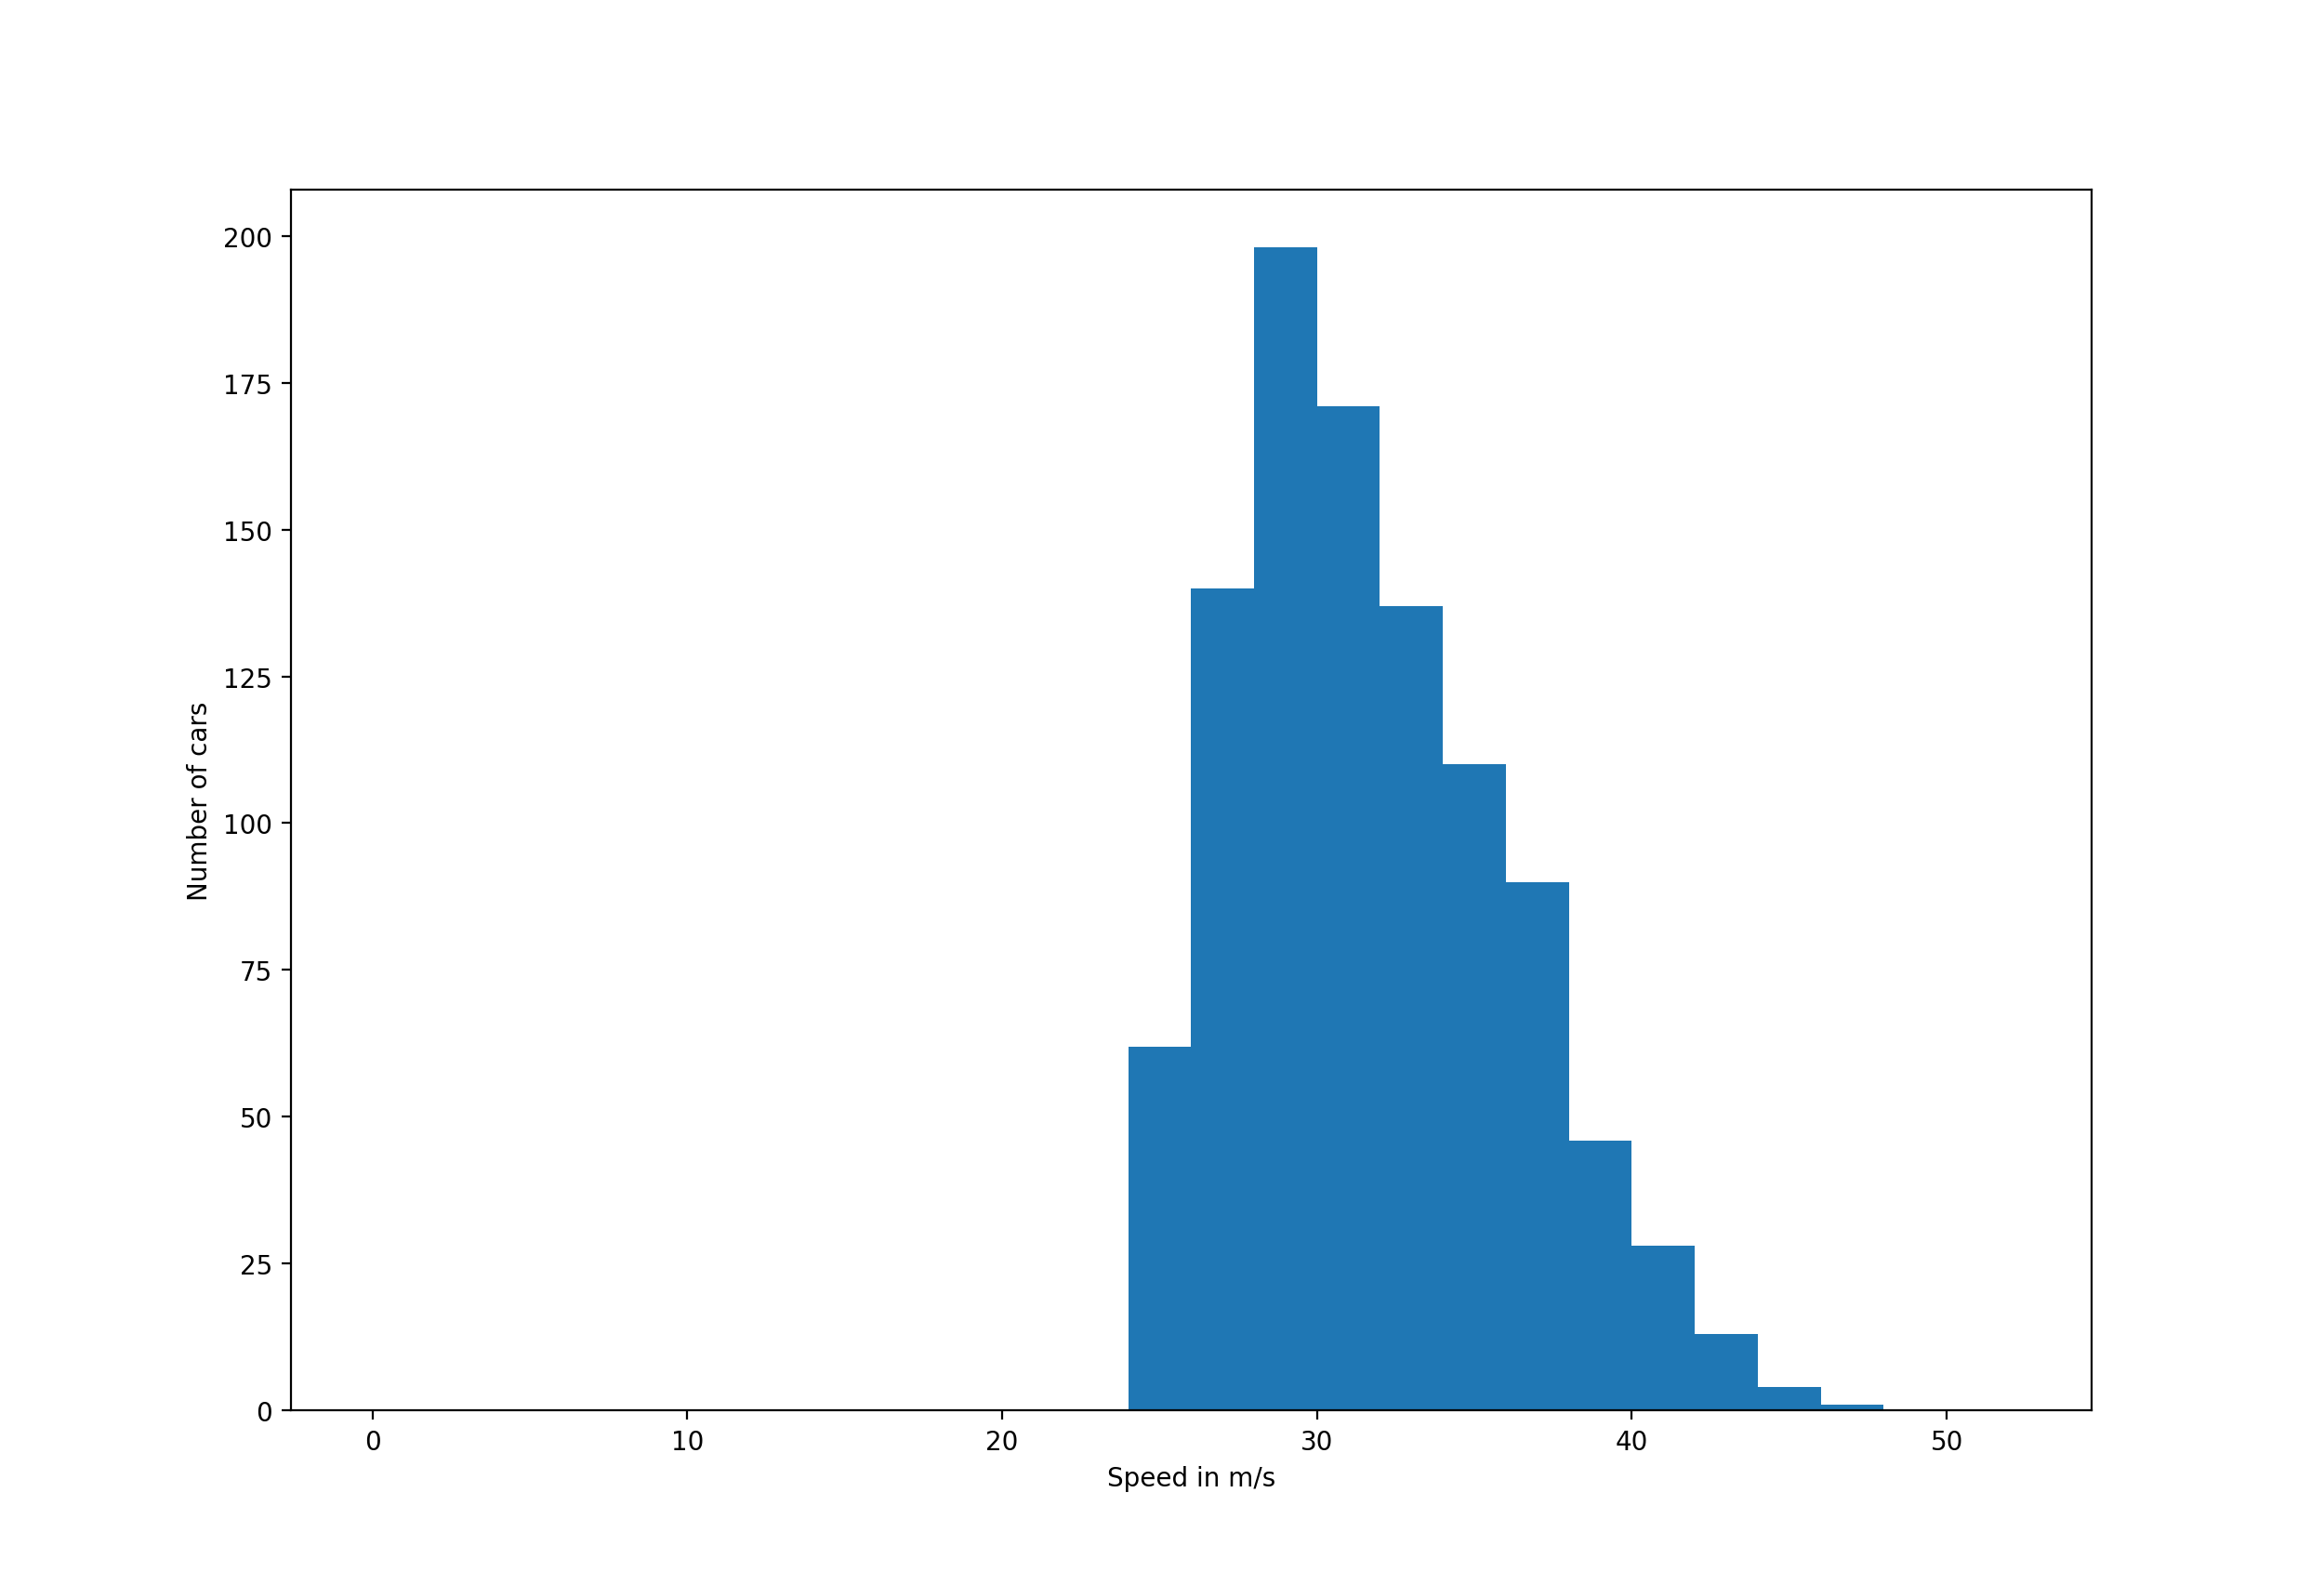
\includegraphics[width=\textwidth] {speed_histo.png}

Often, a histogram will tell the story of the data. Here, you can see
that no one is going less than 24 m/s, but a lot of people travel at
30 m/s. There are a few people who travel over 40 m/s, but there are also a
couple of people who drive much faster than anyone else.

\section{Root-Mean-Squared}

Scientists have a mean-like statistic that they love. It is named
quadratic mean, but most just calls it Root-Mean-Squared, or
RMS.

\begin{mdframed}[style=important, frametitle={Definition of RMS}]

If you have a list of numbers $x_1, x_2, \ldots, x_n$, their RMS
is \index{quadratic mean} \index{root-mean-squared} \index{RMS}

$$\sqrt{\frac{1}{n}\left( x_1^2 + x_2^2 + \ldots + x_n^2 \right)}$$

\end{mdframed}

You are taking the square root of the mean of squares of the samples,
thus the name Root-Mean-Squared.

Using your 12 samples:

\begin{tabular}{c |  c}
  $x$ & $x^2$ \\
  \hline
30.462 & 927.933 \\
29.550 & 873.203\\
29.227 & 854.218\\
37.661 & 1418.351\\
27.899 & 778.354\\
28.113 & 790.341\\
24.382 & 594.482\\
35.668 & 1272.206\\
43.797 & 1918.177\\
31.312 & 980.441\\
37.637 & 1416.544\\
30.891 & 954.254\\
\hline
\multicolumn{1}{r}{Mean of $x^2$} & {1064.875}\\
\multicolumn{1}{r}{RMS} & {32.632}
  \end{tabular}

Why is RMS useful? Let's say that all cars had the same mass $m$, and
you need to know what the average kinetic energy per car is. If you
know the RMS of the speeds of the cars is $v_{rms}$, the average kinetic energy for
each car is

$$k = \frac{1}{2}m v_{rms}^2$$

(You don't believe me? Let's prove it. Substitute in the RMS:

$$k = \frac{1}{2}m \sqrt{\frac{1}{n}\left( x_1^2 + x_2^2 + \ldots + x_n^2 \right)}^2$$

The square root and the square cancel each other out:

$$k = \frac{1}{2}m \frac{1}{n}\left( x_1^2 + x_2^2 + \ldots + x_n^2 \right)$$

Use the distributive property:

$$k = \frac{1}{n} \left( \frac{1}{2} m x_1^2 + \frac{1}{2}m x_2^2 + \ldots + \frac{1}{2}m x_n^2 \right)$$


That is all the kinetic energy divided by the number of cars, which is
the mean kinetic enegy per car. Quod erat demonstrandum! (That is a
Latin phrase that means ``which is what I was trying to
demonstrate''. You will sometimes see ``QED'' at the end of a long
mathematic proof.)

Now you are ready for the punchline: Kinetic energy and heat are the
same thing. Instead of cars, heat is the kinetic energy of molecules
moving around. More on this soon.

Video: Mean, Median, Mode: https://www.youtube.com/watch?v=5C9LBF3b65s



\graphicspath{{../../Chapters/stat_spreadsheets/en_US}}
\chapter{Basic Statistics in Spreadsheets}

When you completed the problems in the last section, you probably noticed
how long it took to compute statistics like the mean, the median,
and variance by hand. Luckily, computers were designed to free us from these
sorts of tedious tasks. The most basic tool for automating
calculations is the spreadsheet program.\index{spreadsheet}

There are lots of spreadsheet programs including Microsoft's Excel and
Apple's Numbers. Any spreadsheet program will work; they are all very
similar. The instructions and screenshots here will be from Google
Sheets -- a free spreadsheet program you use through your web browser.

\section{Your First Spreadsheet}

In whatever spreadsheet program you are using, create a new spreadsheet document.

A spreadsheet is essentially a grid of cells. In each cell you can put data (like numbers or text) and formulas.

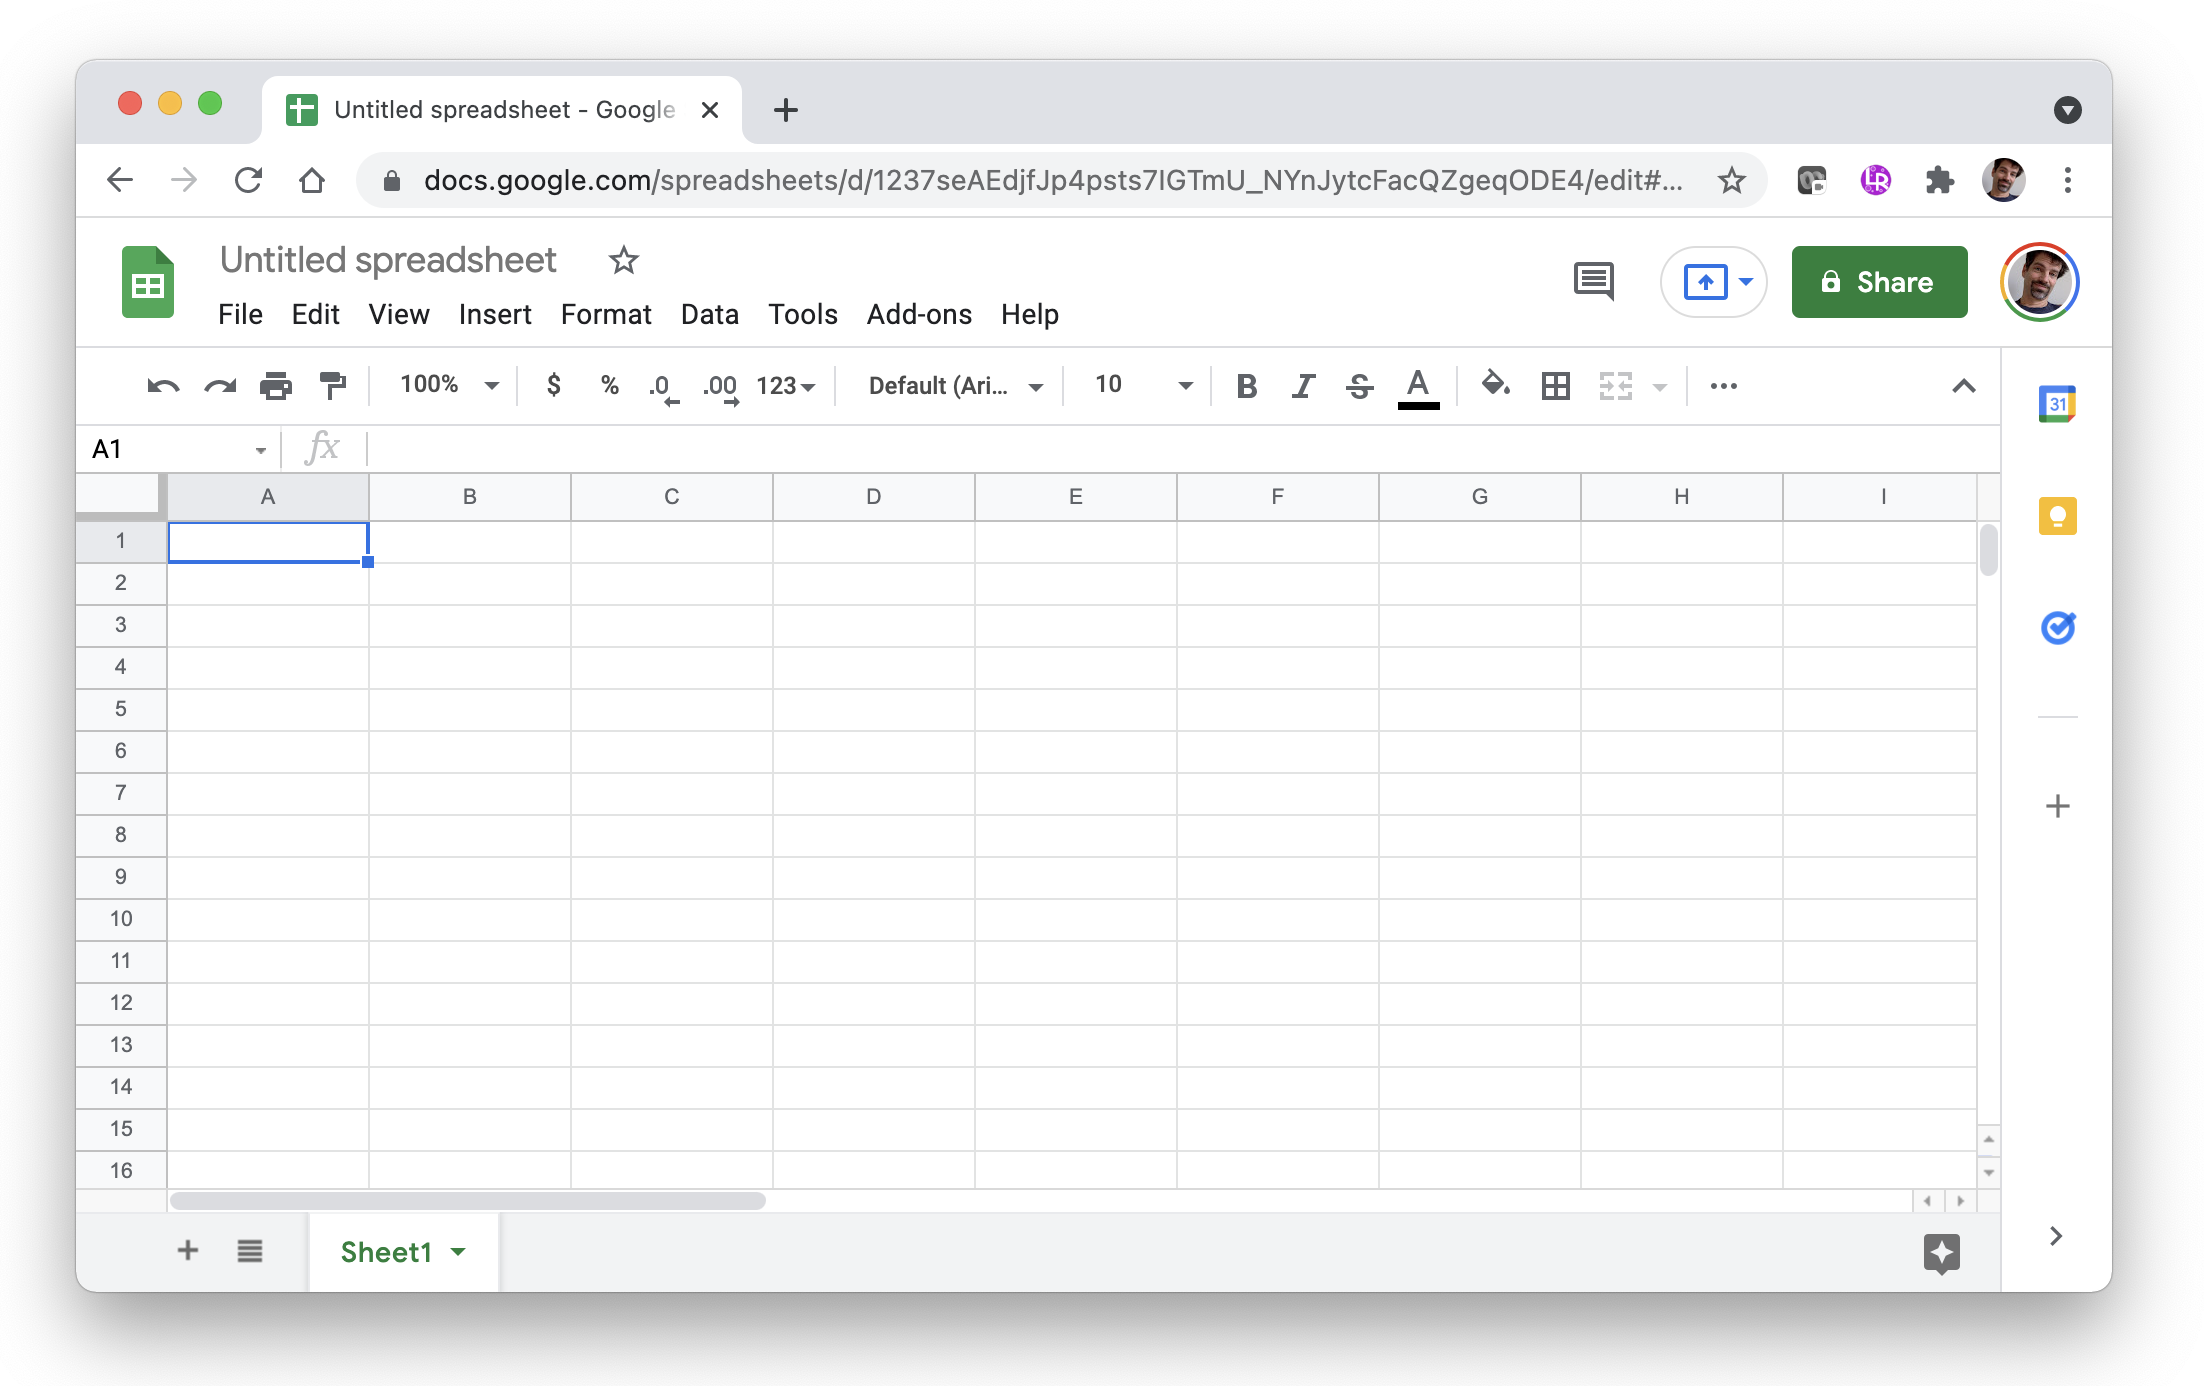
\includegraphics[width=0.6\textwidth]{BlankSheet.png}

Let's put some labels in the column:
\begin{itemize}
\item Select the first cell (A1) and type ``A number''.
\item Select the cell below it (A2) and type ``Another number''.
\item Select the cell below that one (A3) and type ``Their product''.
\item In the next column, type the number 5 in B1 and 7 in B2.
\end{itemize}

It should look like this:

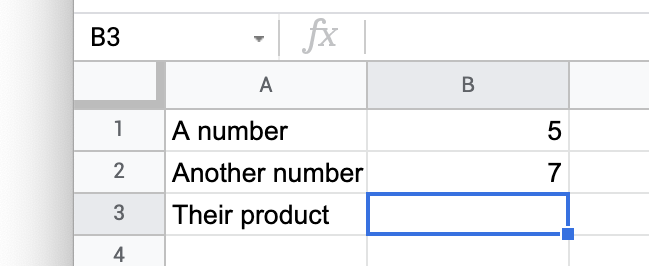
\includegraphics[width=0.5\textwidth]{NoFormulas.png}

Now put a formula in cell B3. Select B3, and type ``= B1 + B2''. The spreadsheet knows this is a formula because it starts with `=`. It will look like this as you type:\index{Spreadsheet!Entering formula}

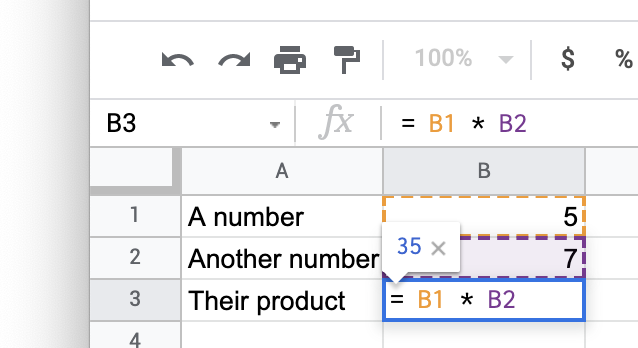
\includegraphics[width=0.5\textwidth]{TypingFirstFormula.png}

When you press Return or Tab, the spreadsheet will remember the formula, but display its value:

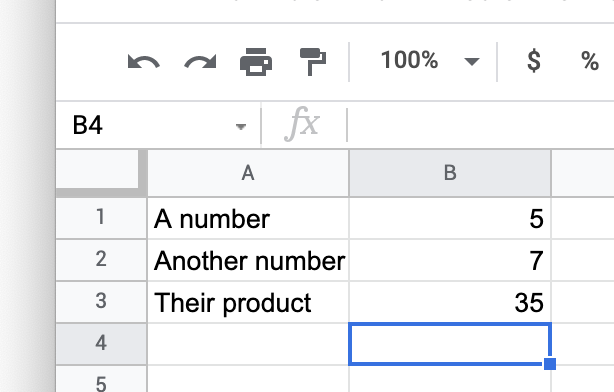
\includegraphics[width=0.5\textwidth]{FirstCalc.png}

If you change the values of cell B1 or B2, the cell B3 will automatically be recalculated. Try it.

\section{Formatting}

Every spreadsheet lets you change the formatting of your columns and cells. They are all a little different, so play with your spreadsheet a little now. Try to do the following:
\begin{itemize}
\item Set the background of the first column to light gray.
\item Right-justify the text in the first column.
\item Make the text in the first column bold.
\item Make the numbers in the second column have one digit after the decimal point.
\end{itemize}

It should look something like this:

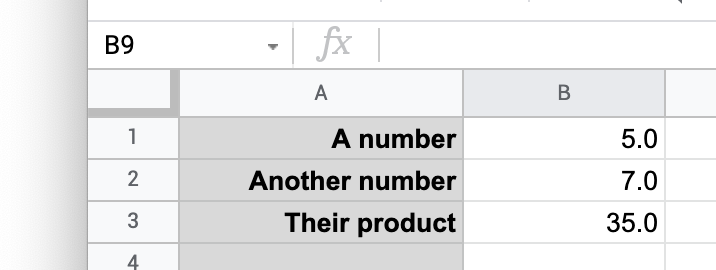
\includegraphics[width=0.6\textwidth]{FirstFormatting.png}

That's a spreadsheet. You have a grid of cells. Each cell can hold a
value or a formula that uses values from other cells. The cells with
formulas automatically update as you edit the values in the other
cells.

\section{Comma-Separated Values}

A lot of data is exchanged in a file format called
\textit{Comma-Separated Values} or just CSV. Each CSV file holds one
table of data. It is a text file, and each line of text corresponds to
one row of data in the table. The data in each column is separated by
a comma. The first line of a CSV is usually the names of the
columns. A CSV might look like this:

\begin{Verbatim}
studentID,firstName,lastName,height,weight
1,Marvin,Sumner,260,45.3
2,Lucy,Harris,242,42.2
3,James,Boyd,261,44.2
\end{Verbatim}

In your digital resources for this module, you should have a file
called \path{1000cars.csv}. It is a CSV with only one column called
``speed''. The first few lines look like this:

\begin{Verbatim}
speed
33.8000
29.9920
34.8699
27.9936
\end{Verbatim}

There is a title line and 1000 data lines.

Import this CSV into your spreadsheet program. In Google Sheets, it looks like this:

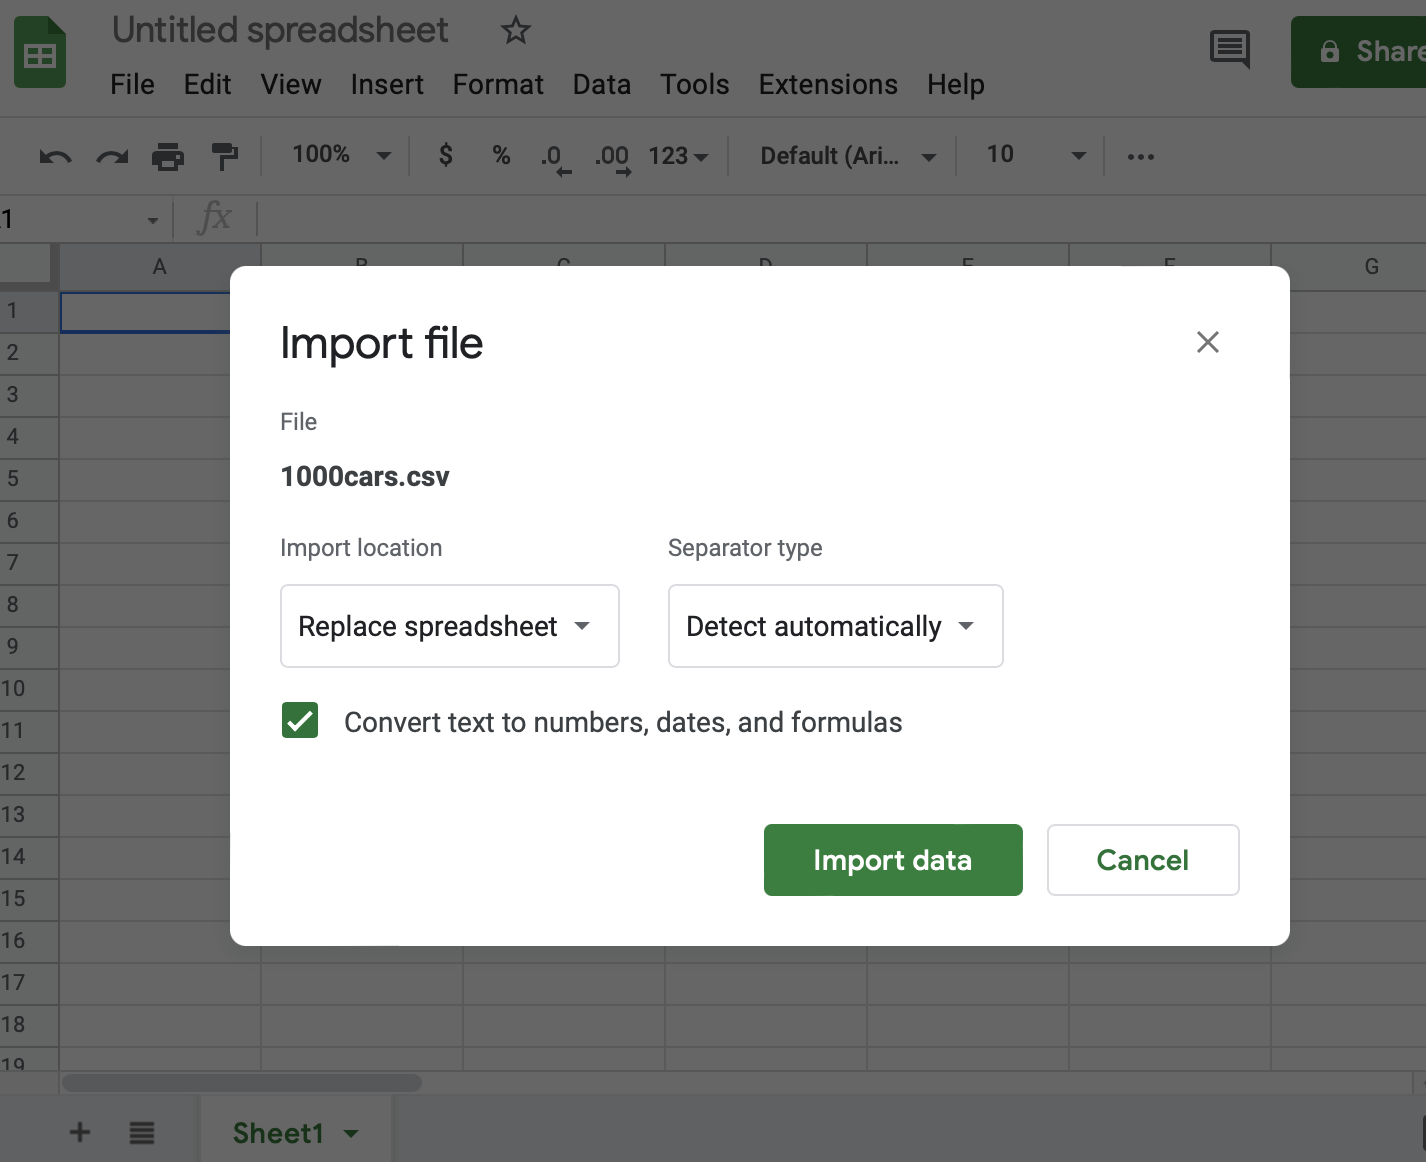
\includegraphics[width=0.5\textwidth]{ImportingCSV.png}

You should see a long, long column of data appear. (Mine goes from cell A2 through A1001.)

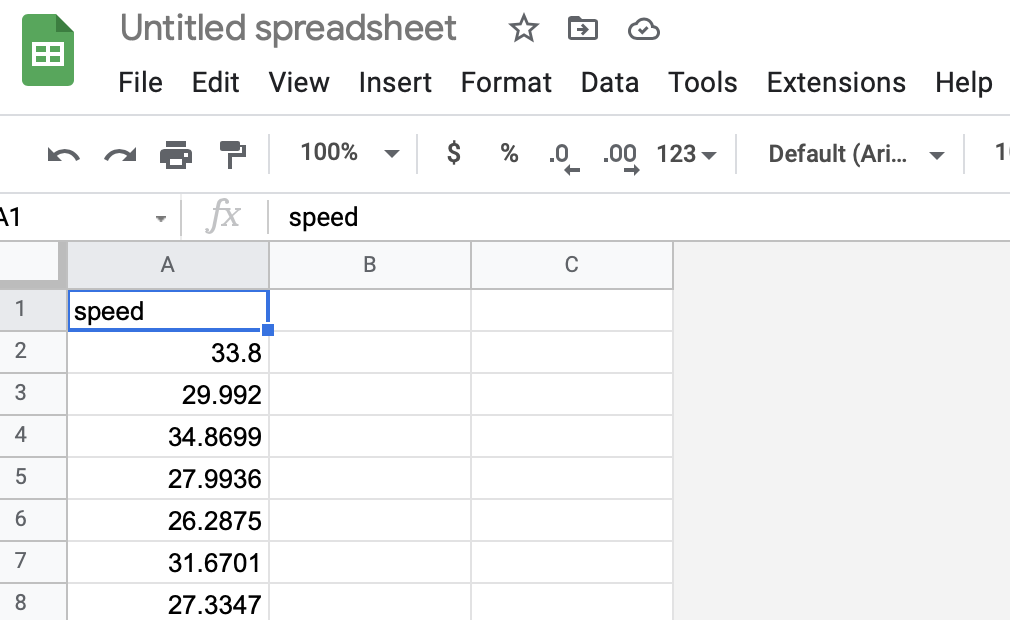
\includegraphics[width=0.5\textwidth]{ImportedCSV.png}

\section{Statistics in Spreadsheets}

Let's take the mean of all 1000 numbers.  In cell B2, type in a label:
``Mean''. (Feel free to format your labels as you wish. Bolding is recommended.)

In cell C2, enter the formula ``=AVERAGE(A2:A1001)''. When
you press return, the cell will show the mean: 31.70441, if done correctly.

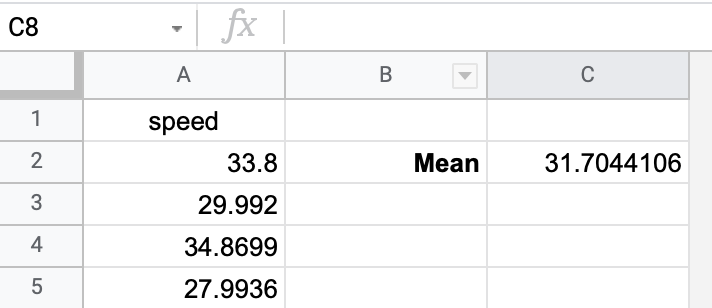
\includegraphics[width=0.4\textwidth]{Spread_mean.png}

Notice that by specifying that the function \pyfunction{AVERAGE} was to
be performed on a range of cells: cells A2 through A1001.

Do the calculations for variance, standard deviation, and median.

\begin{itemize}
\item The function for variance is \pyfunction{VAR}.
\item The function for standard deviation is \pyfunction{STDEV}.
\item The function for median is \pyfunction{MEDIAN}.
\end{itemize}

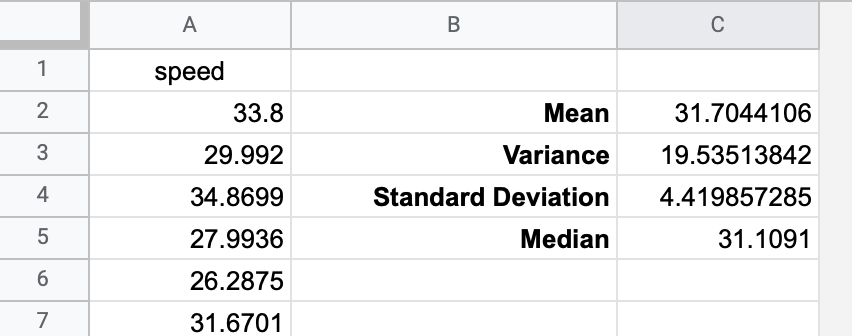
\includegraphics[width=0.4\textwidth]{var_stdev_median.png}

\section{Histogram}

Most spreadsheets have the ability to create a histogram. In Google
Sheets, you select the entire range A2:A1001 by selecting the first
cell and then shift-clicking the last. Then you choose
Insert$\rightarrow$Chart. In the inspector, change the type of the
chart to a histogram. This will get you a basic histogram.
% Add: Define histogram or give example, defined in basic statistics, must come previous

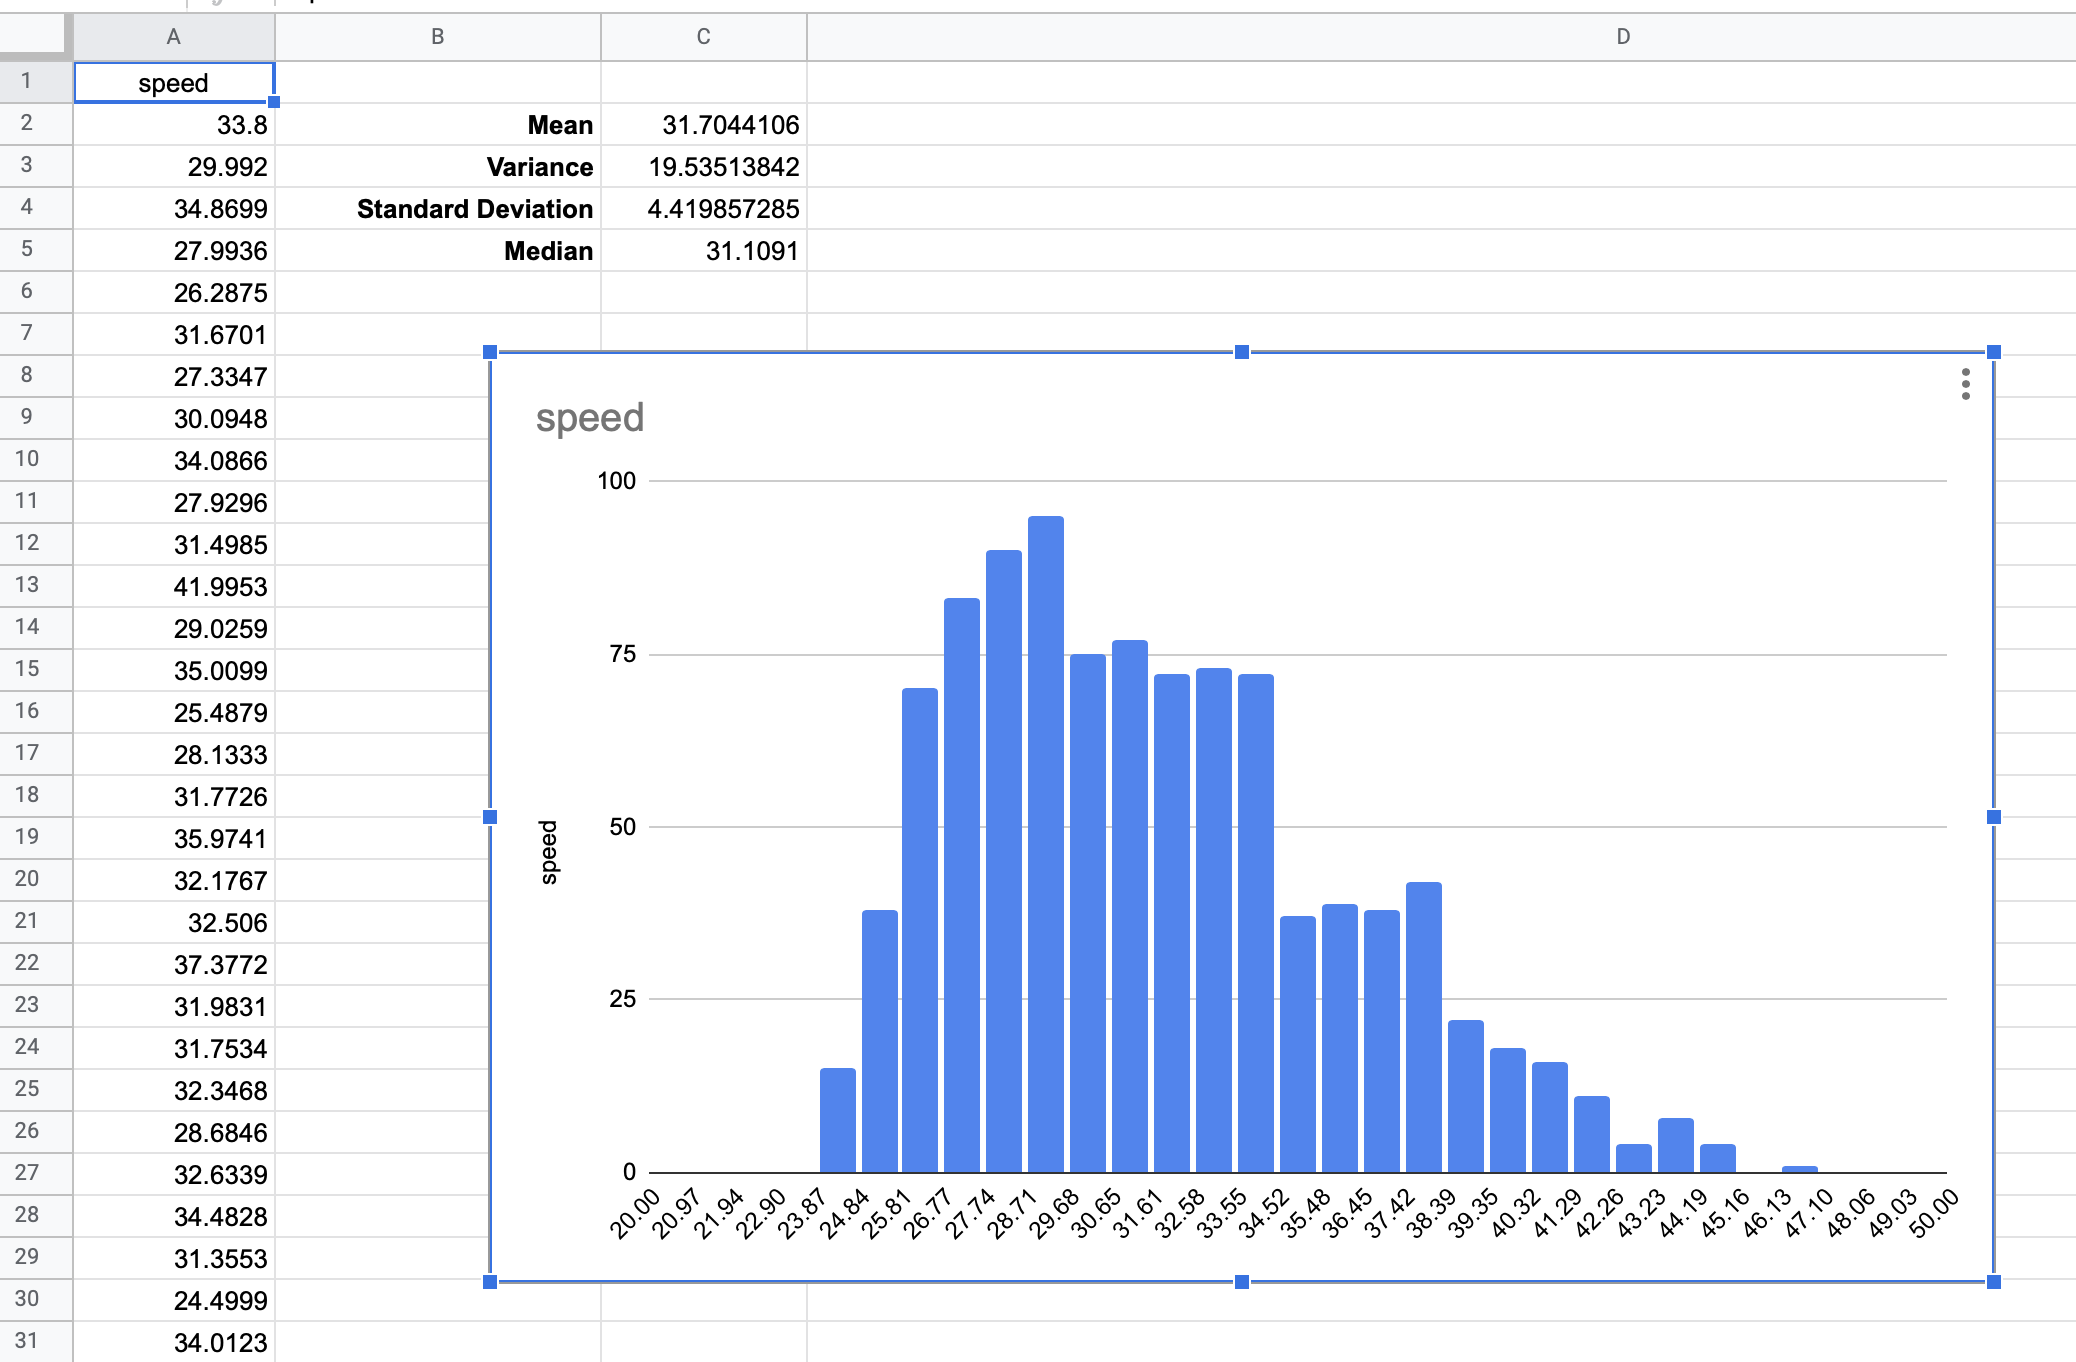
\includegraphics[width=0.7\textwidth]{default_histogram.png}

Play with the formatting to see how unique you can make data. Here is an example:

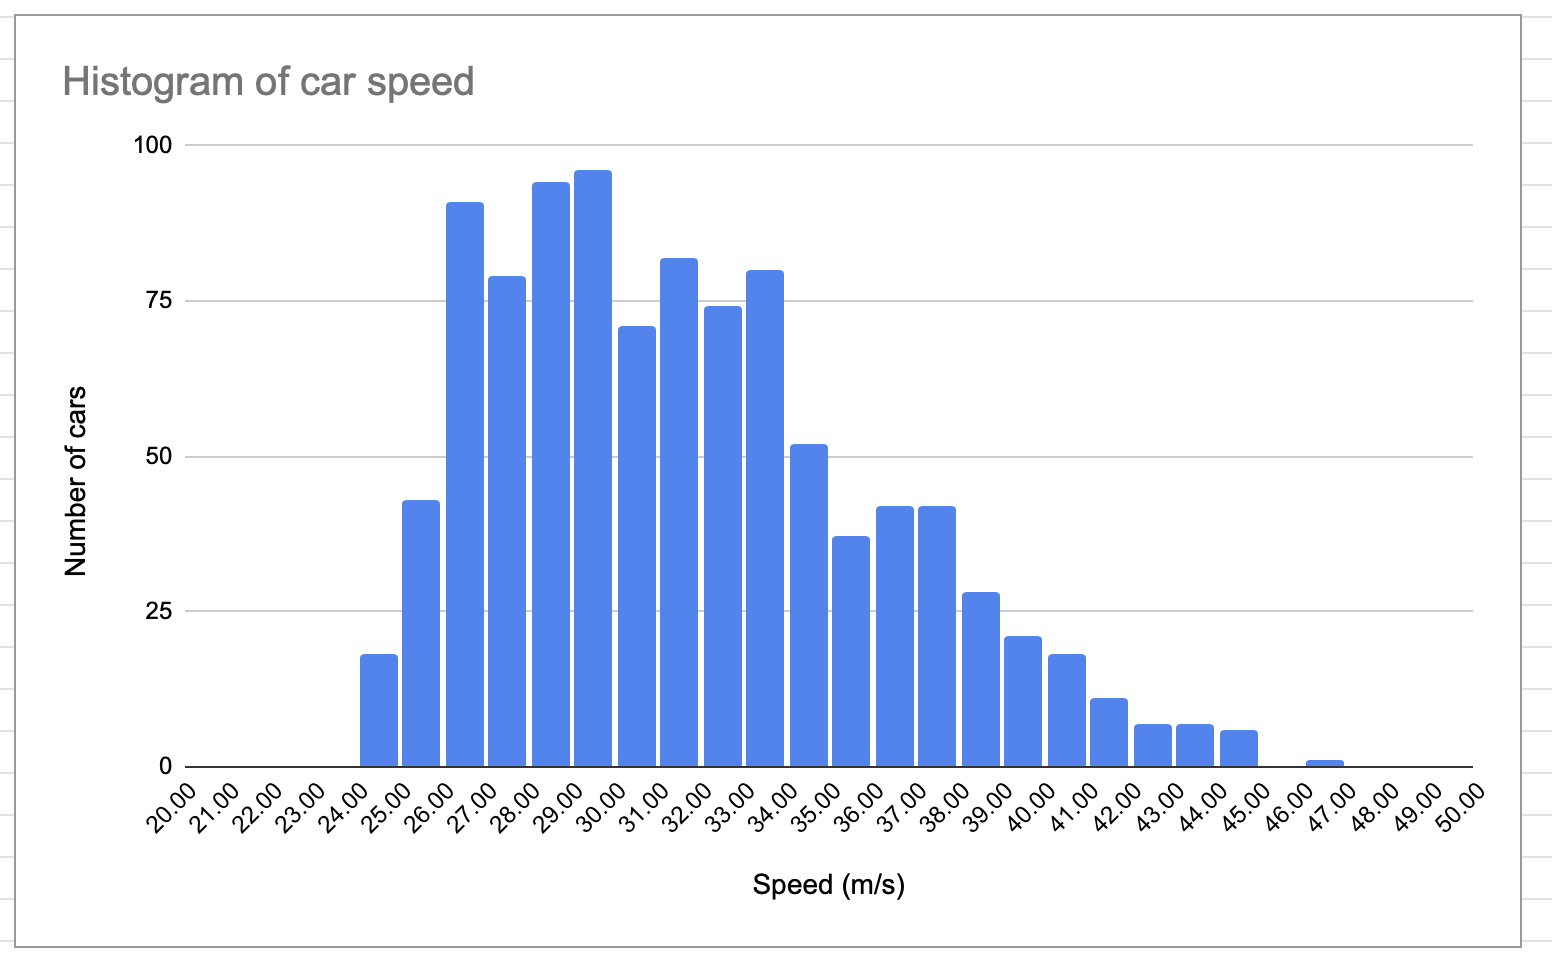
\includegraphics[width=0.8\textwidth]{final_histogram.png}

\begin{Exercise}[title={RMS}, label=rms_spreadsheet]

  In your spreadsheet, calculate the quadratic mean (the root-mean-squared) of the speeds.

  You will need the following three functions:
  \begin{itemize}
  \item \pyfunction{SUMSQ} returns the sum of the squares of a range of cells.
  \item \pyfunction{COUNT} returns the number of cells in a range that contains numbers.
  \item \pyfunction{SQRT} returns the square root of a number.
  \end{itemize}


\end{Exercise}
\begin{Answer}[ref=rms_spreadsheet]

The formula for the RMS is ``=SQRT(SUMSQ(A2:A1001)/COUNT(A2:A1001))''.
% KA: https://www.khanacademy.org/computing/ap-computer-science-principles/data-analysis-101/data-tools/a/learning-from-data-sets

\end{Answer}


\graphicspath{{../../Chapters/dc1/en_US}}
\chapter{Introduction to Electricity}

What happens when you turn on a flashlight? The battery in the
flashlight acts as an electron pump. The electrons flow through the
wires to the lightbulb (or LED). As the electrons pass through the
lightbulb, they excite the molecules within, which gives off light and
heat. (LEDs also give off light and heat, but they give off a lot less
heat.) Then the electrons return to the battery to be pumped around
again.

When electricity is flowing through a copper wire, the protons and
neutrons of the copper stay put while the electrons jump between the
atoms on their way from the battery to the lightbulb and back again.

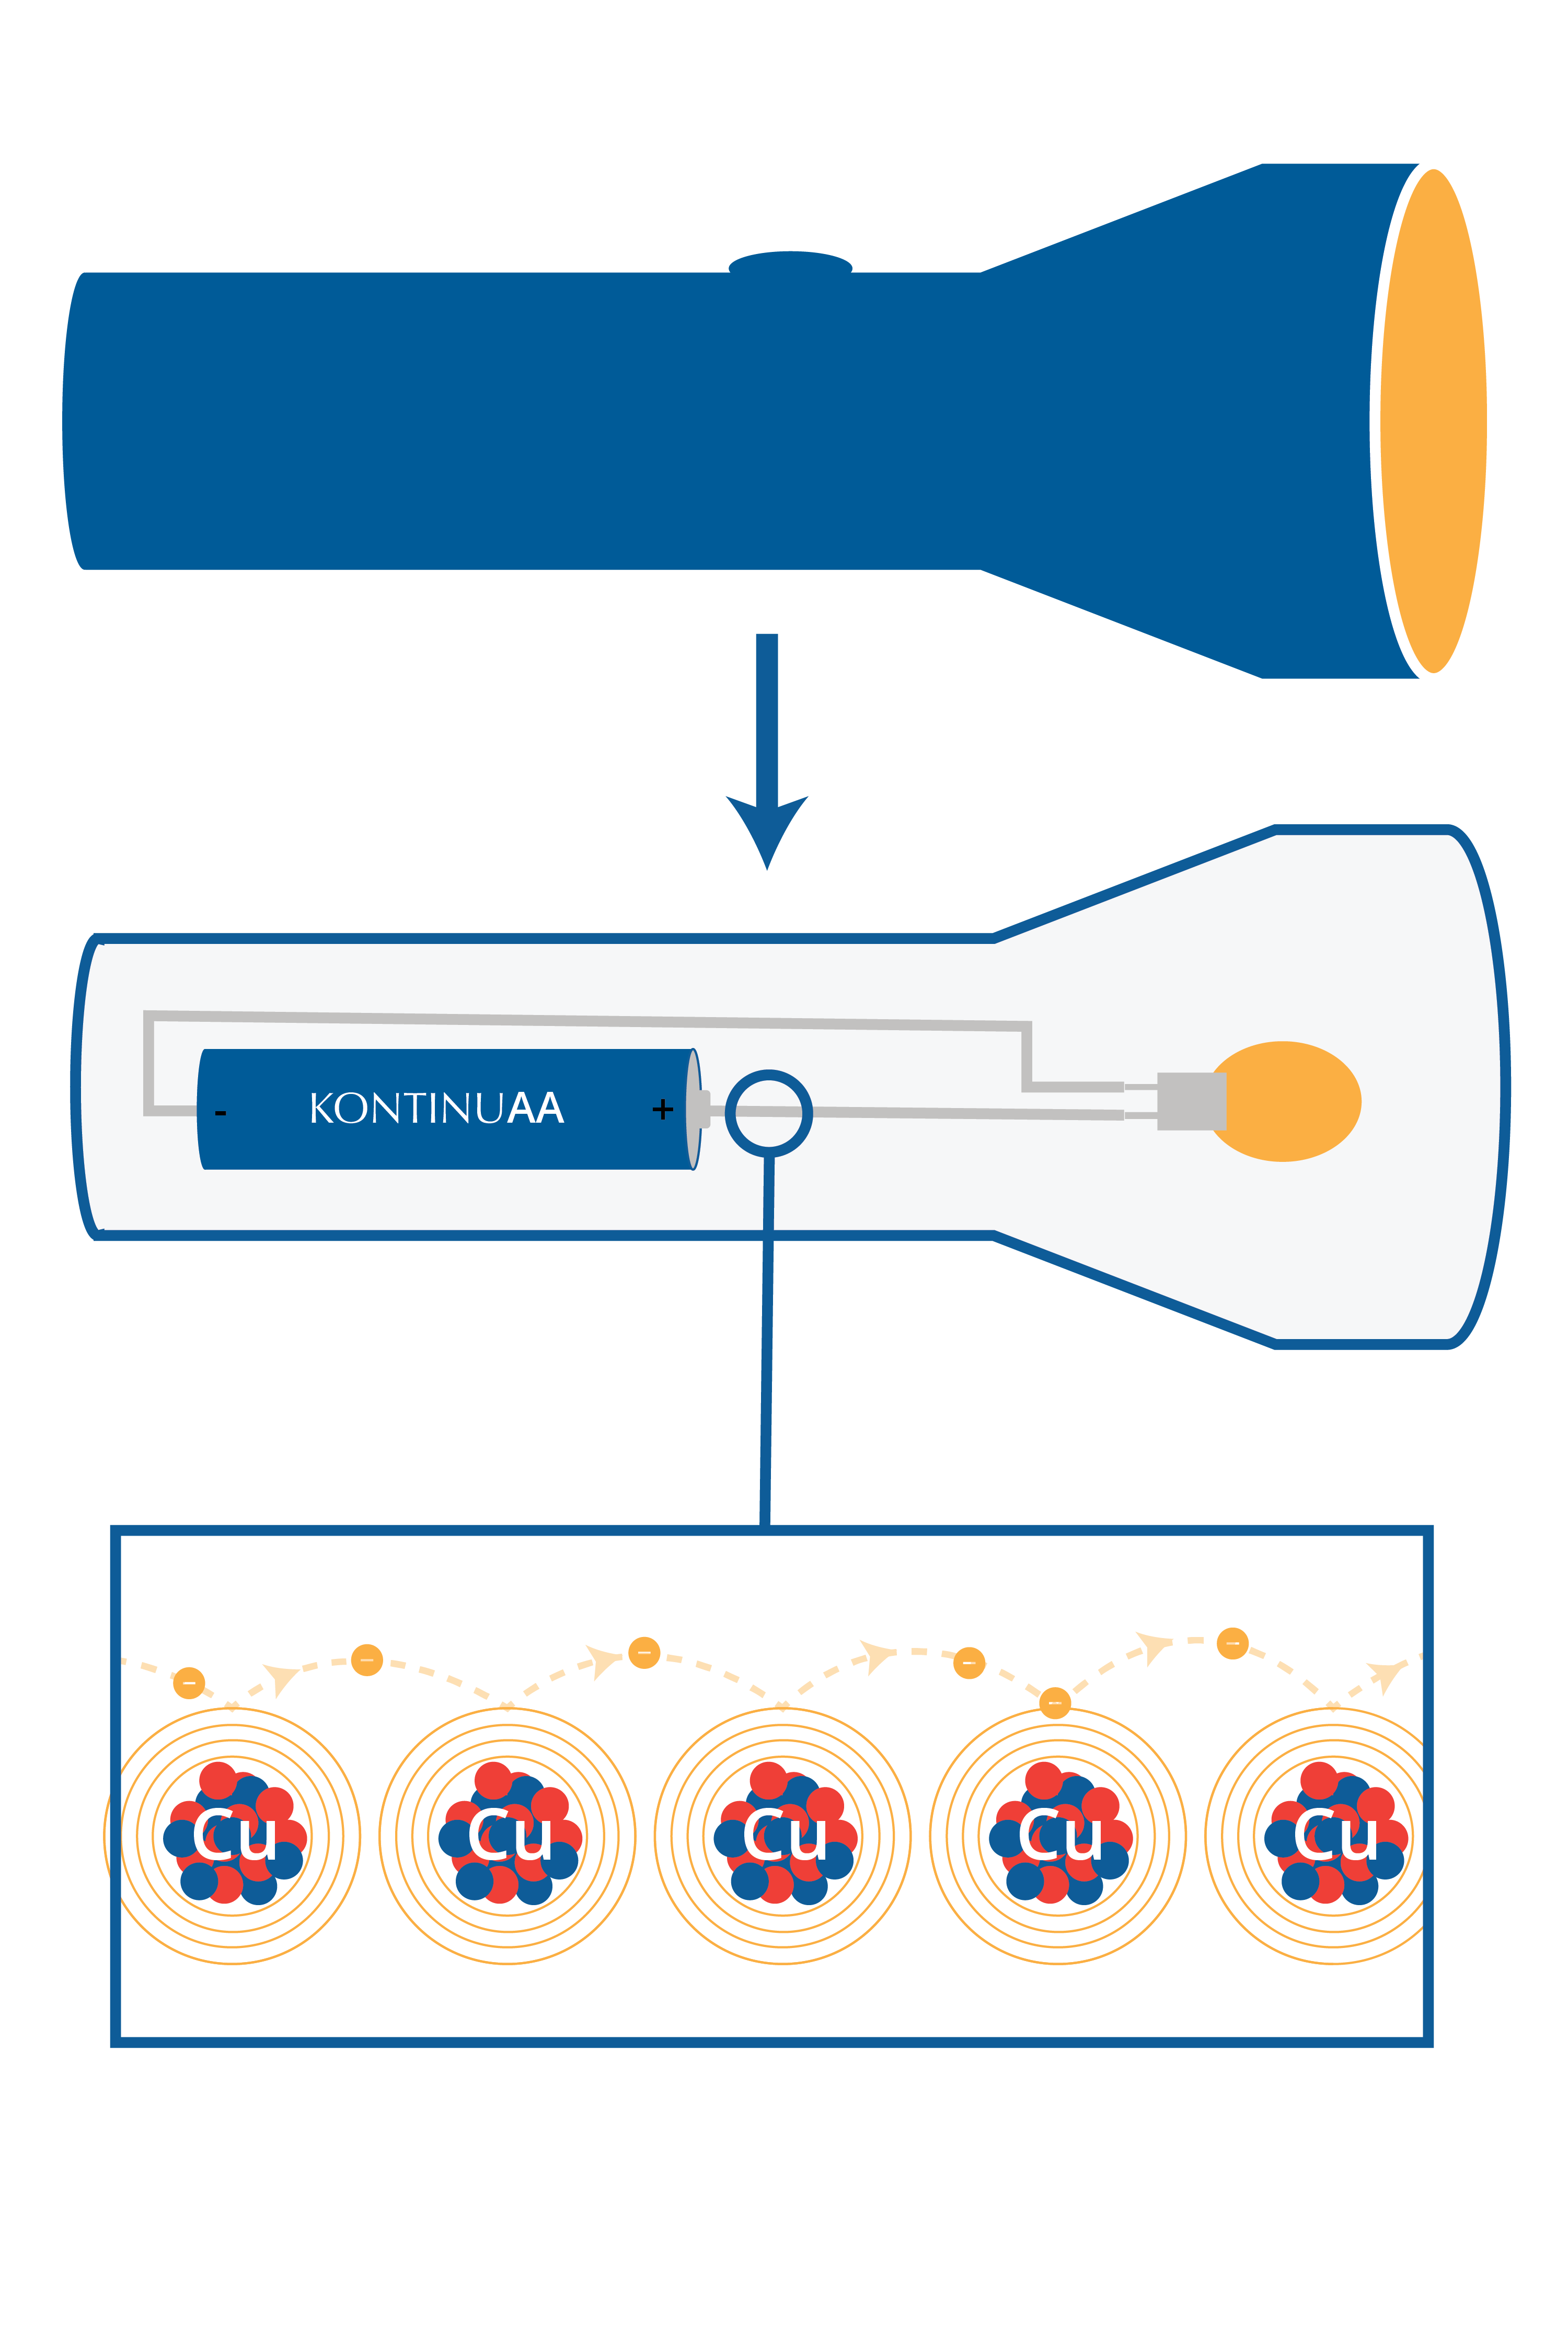
\includegraphics[width=.5\textwidth]{flashlight.png}


In some materials, like copper and iron, electrons are loosely bound
to their nuclei, forming a sea of electrons, which allows energy to flow. These are good \textit{electrical conductors}. In
other materials, like glass and plastic, electrons don't leave their
nuclei easily. Thus, they are terrible electrical conductors -- we call
them \textit{electrical insulators}. For example, the plastic around a
wire is electrical insulation.

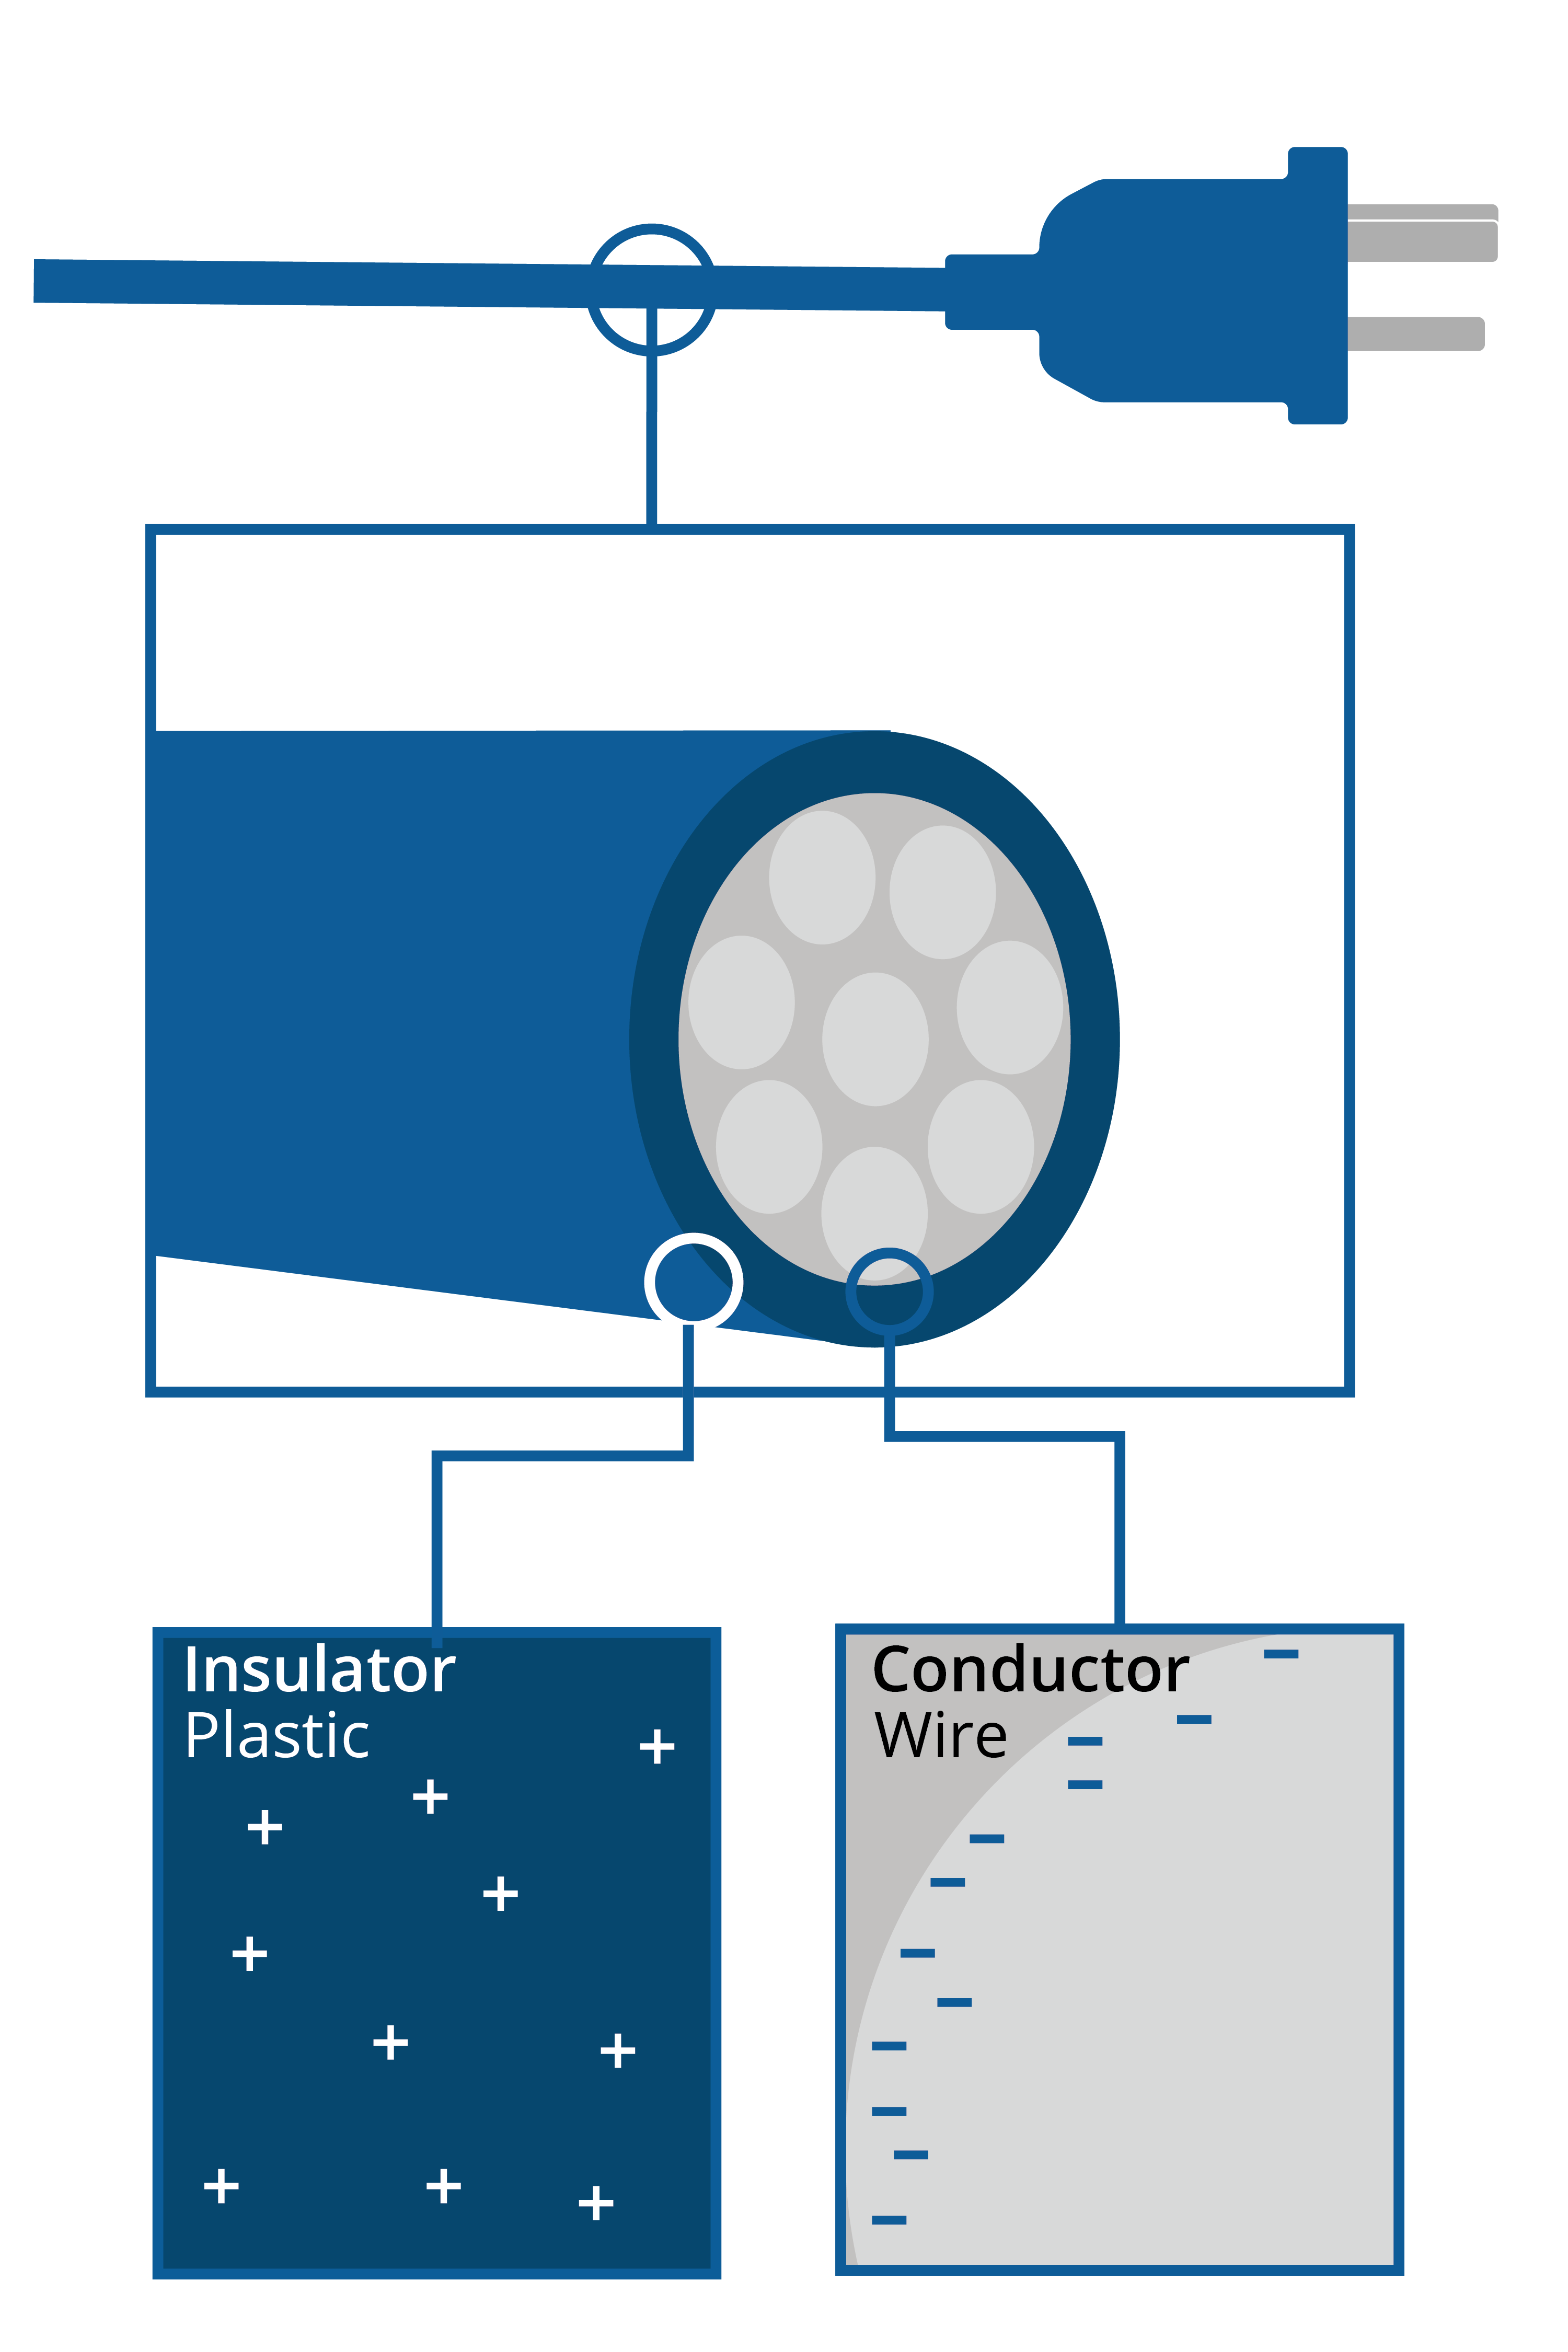
\includegraphics[width=.8\textwidth]{plug.png}

% KA: https://www.khanacademy.org/science/physics/electric-charge-electric-force-and-voltage/charge-electric-force/v/conductors-and-insulators

\section{Units}

Electrons are very small, so to study them, scientists came up with a
unit that represents \textit{a lot} of electrons. 1 \textit{coulomb}
is about 6,241,509,074,460,762,608 electrons.  When 5 coulombs enter one end of the wire every second (and simultaneously 5 coulombs exit the other end), we say ``This wire is carrying 5 amperes of current.''\index{coulombs}

(Truthfully, we usually shorten ampere to just ``amp''.  This is
sometimes a little awkward because we often shorten the word
``amplifier'' to ``amp''. You should be able to tell which is which
from the context.)\index{amp or ampere}

If you look at the circuit breakers or fuses for your home's
electrical system, you'll see that each one is rated in amps.  For
example, maybe the circuit that supplies power to your kitchen has a 10
amp circuit breaker. If for some reason, more than 10 amps tries to
pass through that wire, the circuit breaker will turn off the whole
circuit.

When it is on, your flashlight pushes about 1 amp of current
through the lightbulb(When it is off, there is no current in the
lightbulb).

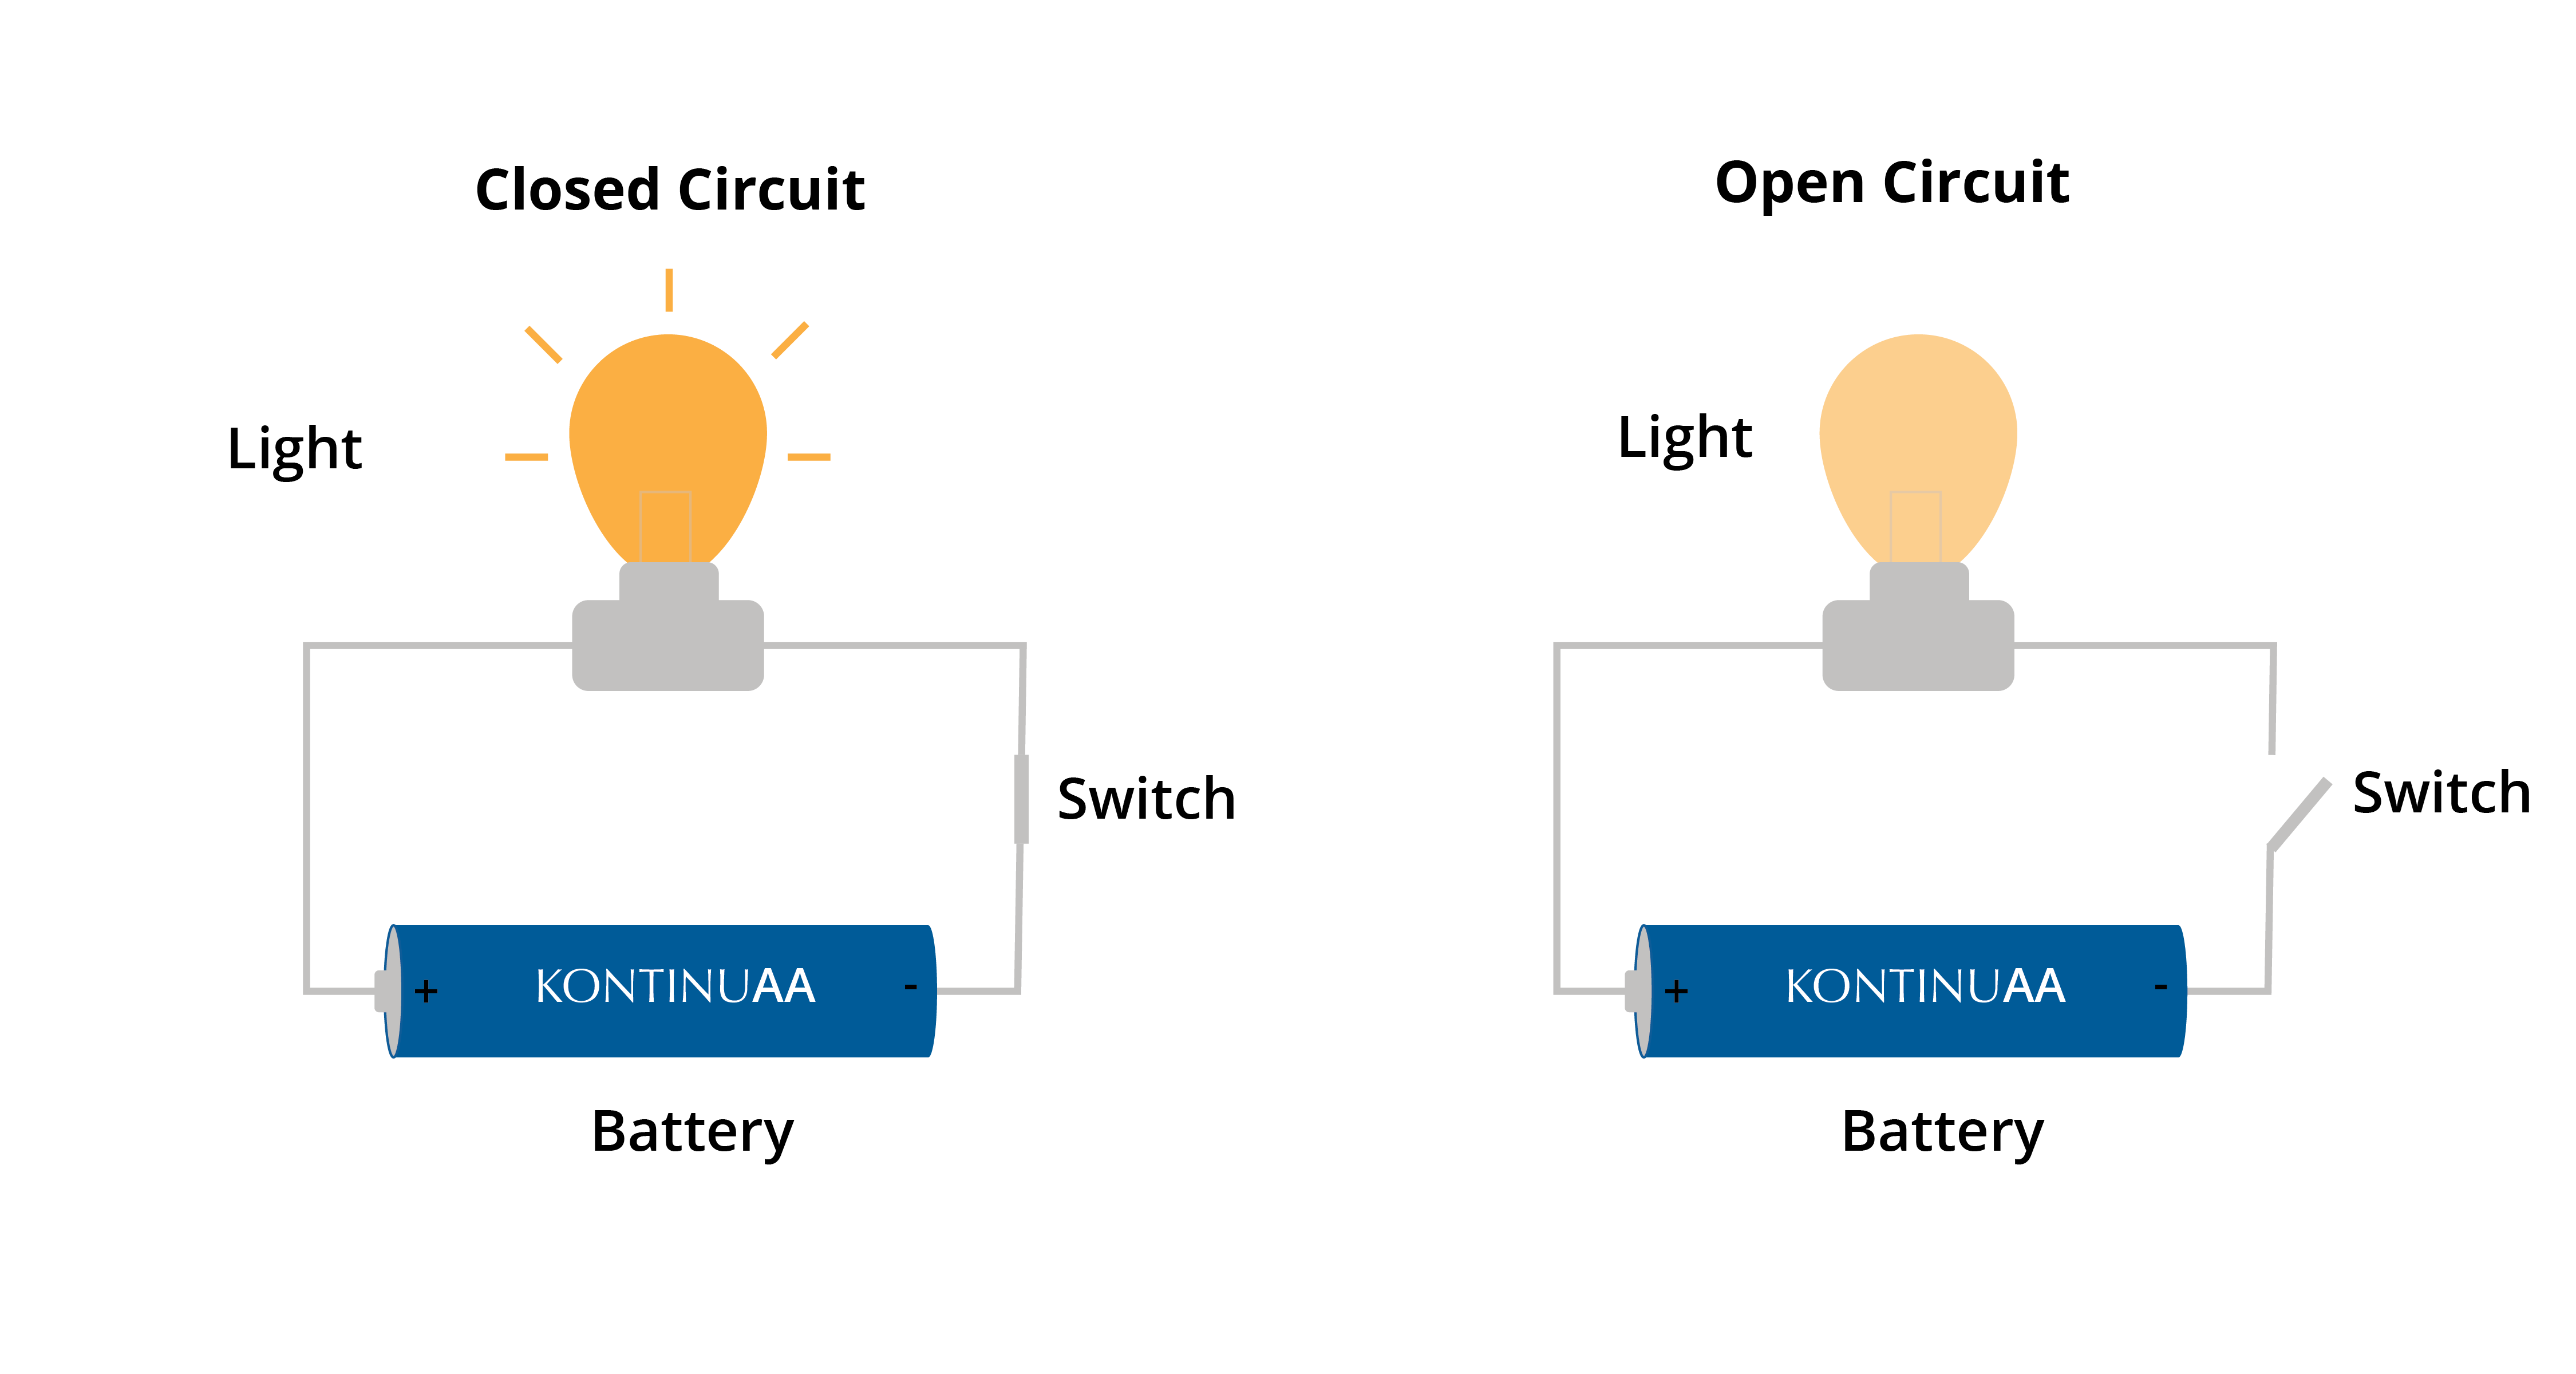
\includegraphics[width=0.8\textwidth]{Circuit_OnOff.png}

The lightbulb creates \textit{Resistance} that the current pushes
through.\index{resistance} Think of it like plumbing: The current is the amount of water
passing through a pipe. The resistance is something that tries to stop
the current -- like a ball of hair. The battery is what allows
 the current to push through the resistance; we call that
pressure \textit{voltage}.\index{voltage}

\section{Circuit Diagrams}

Here is a circuit diagram of your flashlight:

\begin{circuitikz}
\draw (0,0) to[battery1,invert,l=$3V$] ++(0,3)
to [switch,i=1A] ++(3,0)
to [lamp=$1\Omega$,bipoles/length=0.9cm] ++(0,-3) -- (0,0);
\end{circuitikz}

The lines are wires.  The symbols that we  will use:

\begin{tabular}{c c c c}
  Battery & Switch & Lamp & Resistor \\
\begin{circuitikz}
\draw (0,0) to[battery1] (2,0); 
\end{circuitikz}
&
\begin{circuitikz}
\draw (0,0) to[lamp,bipoles/length=0.9cm,l=$3 \Omega$] (2,0); 
\end{circuitikz}
&
\begin{circuitikz}
\draw (0,0) to[switch,/tikz/circuitikz/bipoles/length=1.0cm] (2,0); 
\end{circuitikz}
&
\begin{circuitikz}
\draw (0,0) to[R,  l=$3 \Omega$] (2,0); 
\end{circuitikz} \\
\end{tabular}

The battery pushes the electrons from one end and pulls them back in at the other, so the circuit must go around in a circle for the current to flow. This is why the current stops flowing when the switch breaks the circuit.

You can think of a switch as having zero resistance when it is closed and infinite resistance when it is open.


For our purposes, a lamp is just a resistor that gives off light.
% KA: https://www.khanacademy.org/science/high-school-physics/dc-circuits/electric-power-and-dc-circuits/a/circuit-introduction

\section{Ohm's Law}

Resistance is measured in \textit{ohms}, and we use a Greek capital omega for that: $\Omega$  

Voltage is measured in
\textit{volts}.\index{ohms}\index{volts}

\begin{mdframed}[style=important, frametitle={Ohm's Law}]\index{Ohm's law}
  Whenever a voltage $V$ is pushing a current $I$ through a resistance of $I$, the following is true:

  $$V = IR$$

  where $V$ is in volts, $I$ is in amps, and $R$ is in ohms.
\end{mdframed}
% KA: https://www.khanacademy.org/science/physics/circuits-topic/circuits-resistance/v/circuits-part-1

\section{Power and Watts}

\begin{mdframed}[style=important, frametitle={Joule's Law}]\index{Joule's law}

  When a current $I$ is passing through a resistance $R$, the power consumed is
  
  $$W = I^2 R$$

  where $W$ is in watts, $I$ is in amps, and $R$ is in ohms.
\end{mdframed}

Of course $V = IR$, so we can extend this to:

$$W = I^2 R = I V = \frac{V^2}{R}$$

Your flashlight's batteries provide about 3 volts. How much
battery power is the flashlight using when it is on? The power (in
watts) produced by the battery is the product of the voltage (in
volts) and the current (in amps). So your flashlight is giving off $3
volts \times 1 amp = 3 watts$ of power. Some of that power is given
off as light, some as heat.\index{watts}

A watt is 1 joule of energy per second. We say that a watt is a
measure of \textit{power}.

When we talk about how much energy is stored in a battery, we use a
unit like a kilowatt-hour. A kilowatt-hour is equivalent to 3.6 million
joules.

\section{Another great use of RMS}

In many electrical problems, the voltage fluctuates a lot.  For
example, the fluctuations in voltage makes the sound that comes out of an
audio speaker.

You can use the root-mean-squared of the voltage to figure out the average power
your speaker is consuming.

Let's say that the RMS of the voltage you are sending to the speaker is $V_{rms}$
and the resistance of the speaker is $R$ ohms, then the power consumed
by the speaker is:

$$P = \frac{V_{rms}^2}{R}$$

Similarly, if you know the RMS of the current you are pushing through
the speaker is $I_{rms}$, then the power consumed by the speaker is:

$$P = I_{rms} R$$

\section{Electricity Dangers}

Large amounts of electricity moving through your body can hurt or even kill
you. You must be careful around electricity.

However, your body is not a very good conductor, so low-voltage
systems (like a flashlight) don't have enough voltage to move significant amounts of
current through your body.

However, the  electricity in a power outlet has much more voltage. The voltage
in these outlets is fluctuating between positive and negative, so we
call it \textit{Alternating Current} or AC.
% ADD: Introduce difference between AC and dc

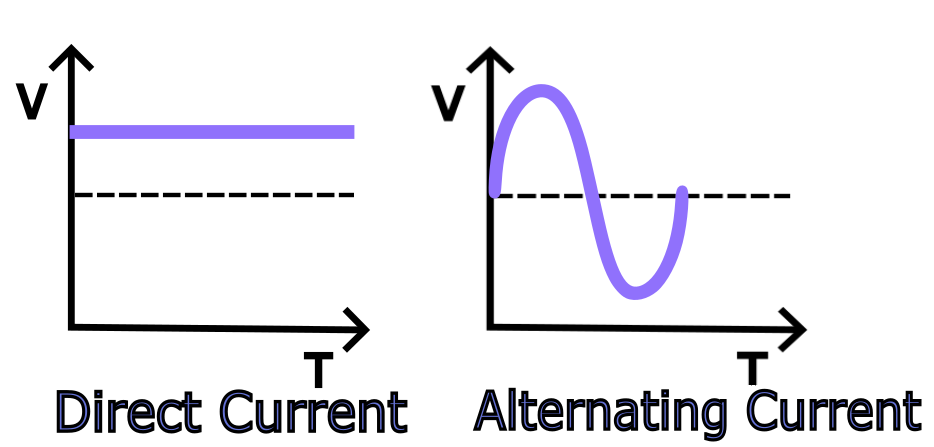
\includegraphics[width=1\textwidth]{AC_vs_DC.png}

In most countries, the RMS of the voltage between 110 and 240 V. (The
peak voltage is always $\sqrt{2}$ times the RMS value. In the US, for
example, people say ``Our outlets supply 120 V.'' They mean that the
RMS of the voltage difference between the wire and the earth is 120V.
The peak voltage is almost 170V.)

How much current can a human handle? Not much. You can barely feel 1
mA moving through your body, but at 16 mA, your muscles will clench
and you won't be able to relax them -- many people die from
electrocution because they grab a wire which pushes enough current
through their body to prevent them from letting go of the wire.  At 20
mA, a human's respiratory muscles become paralyzed.

The fuse breaker in a house will often allow 20 A to flow through the
circuit before it shuts off the power: Always, always, always shut off
the power before touching any of the wiring in your house.

While water is actually a mediocre conductor, it can still deliver enough current
to kill you. If you see a wire in a puddle, you should not touch the
puddle. Interestingly, because of the salt, sea water is more than
100 times better at conducting electricity than the water you drink.
% ADD: Sea of electrons makes a good conductor

% 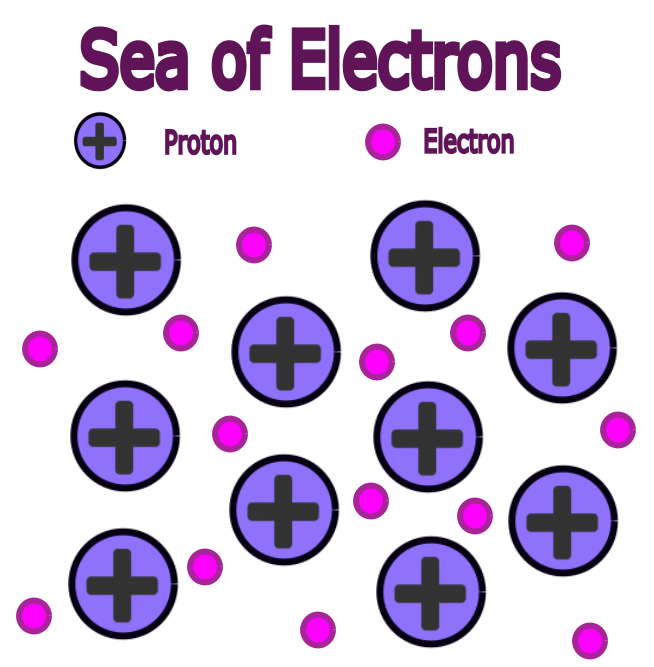
\includegraphics[width=0.8\textwidth]{Sea_Electrons.png}

If you hold a wire in each hand, how many Ohms of resistance will your
body have? Once it gets past your skin, you will look like a bag of
salt water to the electricity. After the skin, your body will have a
resistance of about 300$\Omega$. However, the skin is a pretty good
insulator. If you have dry, calloused hands, your skin may add a
100,000$\Omega$ to the resistance.

% KA: https://www.khanacademy.org/science/in-in-class10th-physics/in-in-electricity/in-in-electric-power-and-heating-effect-of-current/v/electric-power-energy


\graphicspath{{../../Chapters/dc_circuits/en_US}}
\chapter{DC Circuit Analysis}

In the most basic circuit, you have only a battery and a resistor:



\begin{circuitikz}
\draw (0,0) to[battery1,invert,l=$6V$] ++(0,3)
to ++(3,0)
to [R=$3\Omega$, /tikz/circuitikz/bipoles/length=1.0cm,i=2A] ++(0,-3) -- (0,0);
\end{circuitikz}

For this situation, you only need Ohm's Law: $V = I R$.  In this case, $6V = 3\Omega \times 2A$.
% ADD: Define Ohm's Law
\begin{Exercise}[title={Ohm's Law}, label=ohms_check]

  How many amps are going around the circuit?
  
  \vspace{1cm}

\begin{circuitikz}
\draw (0,0) to[battery1,invert,l=$24V$] ++(0,3)
to ++(3,0)
to [R=$6\Omega$, /tikz/circuitikz/bipoles/length=1.0cm,i={? A}] ++(0,-3) -- (0,0);
\end{circuitikz}

  
\end{Exercise}
\begin{Answer}[ref=ohms_check]

  $V = I R$ so $I = \frac{V}{R} = \frac{24V}{6\Omega} = 4A$.
  
\end{Answer}
% KA: https://youtu.be/F_vLWkkOETI

\section{Resistors in Series}

When you have two resistors wired together in a long line, we say they
are ``in series.''  If you have two resistors $R_1$ and $R_2$ wired in
series, the total resistance is $R_1 + R_2$.

In this diagram, for example, the total resistance is $5\Omega$.

\begin{circuitikz}
\draw (0,0) to[battery1,invert,l=$10V$] ++(0,5)
to ++(3,0)
to [R=$3\Omega$] ++(0,-2.5)
to [R=$2\Omega$] ++(0,-2.5) -- (0,0);
\end{circuitikz}

The current flowing through the circuit, then, is $10/5 = 2A$.

By Ohm's law, the voltage drop across the upper resistor is $I R = 2A \times 3\Omega = 6V$.

The voltage drop across the lower resistor is $I R = 2A \times 2\Omega = 4V$.

Notice that the battery pumps the voltage up to $10V$, then the two
resistors drop it by exactly $10V$. This is known as ``Kirchhoff's
Voltage Law'':
% KA: https://youtu.be/4rsswT_Rv1M

\begin{mdframed}[style=important, frametitle={Kirchhoff's Voltage Law}]\index{Kirchhoff's voltage law}
As you make a loop around a circuit, the sum of the voltage increase
must equal the sum of the voltage decrease.
\end{mdframed}

The negative end of the battery is connected to ``ground''\index{index} (it has zero voltage). We can then draw a diagram with the
voltages (That symbol in the lower right represents a connection to ground).

\begin{circuitikz}
\draw (0,0) to[battery1,invert,l=$6V$] ++(0,5) 
to [-*] ++(3,0) node[anchor=west] {10V}
to [R=$3\Omega$,-*] ++(0,-2.5) node[anchor=west] {4V}
to [R=$2\Omega$,-*] ++(0,-2.5) node[anchor=west]{0V} node[ground]{} --(0,0);
\end{circuitikz}


\begin{Exercise}[title={Resistors In Series}, label=series_resistor]

  What is the current going around the circuit?
  
  What is the voltage drop across each resistor?
  
  \vspace{1cm}
\begin{circuitikz}
\draw (0,0) to[battery1,invert,l=$16V$] ++(0,5) 
to [-*] ++(3,0) node[anchor=west] {16V}
to [R=$5\Omega$,-*] ++(0,-2.5) node[anchor=west] {?}
to [R=$3\Omega$,-*] ++(0,-2.5) node[anchor=west]{0V} node[ground]{} --(0,0);
\end{circuitikz}


\end{Exercise}
\begin{Answer}[ref=series_resistors]

  There is a total resistance of $8\Omega$, so your 16V will push 2A
  of current around the circuit.

  2A going through a $5\Omega$ resistor represents a 10V drop.

  2A going through a $3\Omega$ resitor represents a 6V drop.
  
\end{Answer}


\section{Resistors in Parallel}

Observe the following circuit. Note that the current can go two different paths.

\begin{circuitikz}
\draw (0,0) to[battery1,invert,l=$12V$] ++(0,3)
to ++(3,0)
to [R=$2\Omega$, /tikz/circuitikz/bipoles/length=1.0cm] ++(0,-3) -- (0,0);
\draw (3,3) -- (5,3)
to [R=$3\Omega$, /tikz/circuitikz/bipoles/length=1.0cm] ++(0,-3) -- (3,0);
\end{circuitikz}

There is 12 volts pushing current through both resistors. So 6A will
go through the 2$\Omega$ resistor and 4A will go through the 3$\Omega$
resistor. Note that even though there is a path of least resistance (2$\Omega$), the current is still devided evenly among both branches.

\begin{circuitikz}
\draw (0,0) to[battery1,invert,l=$12V$] ++(0,3)
to ++(3,0)
to [R=$2\Omega$, /tikz/circuitikz/bipoles/length=1.0cm,i=6A] ++(0,-3) -- (0,0);
\draw (3,3) -- (5,3)
to [R=$3\Omega$, /tikz/circuitikz/bipoles/length=1.0cm,i=4A] ++(0,-3) -- (3,0);
\end{circuitikz}

Thus, a total of 10 A will be going through the battery.

Imagine you are a battery. You can't see that you have two resistors.
What does it feel like to you? $\frac{V}{I} = R$, and $V= 12$ and $I =
10$. This means the effective resistance of the two resistors in parallel is
$\frac{12}{10}$ or $\frac{6}{5} \Omega$.

\begin{mdframed}[style=important, frametitle={Resistance in Parallel}]\index{resistance!in parallel}
If you have several resistances $R_1, R_2, \ldots, R_n$ wired in
parallel, their effective resistance $R_t$ is given by

$$\frac{1}{R_t} = \frac{1}{R_1} + \frac{1}{R_2} + \ldots + \frac{1}{R_n}$$

\end{mdframed}

In our example:

$$\frac{1}{R_t} = \frac{1}{2} + \frac{1}{3} = \frac{5}{6}$$

Thus, $R_t =  \frac{6}{5}\Omega$.

\begin{Exercise}[title={Resistors In Parallel}, label=parallel_resistors]

  What is the current going through the battery?
  What is the drop over the $4\Omega$ resistor?
  What is the current in each branch?

  \vspace{1cm}

  \begin{circuitikz}
\draw (0,0) to[battery1,invert,l=$12V$] ++(0,3)
to [R=$4\Omega$, /tikz/circuitikz/bipoles/length=1.0cm] ++(3,0) node [yshift=0.3cm] {? V}
to [R=$6\Omega$, /tikz/circuitikz/bipoles/length=1.0cm,i={? A}] ++(0,-3) node[ground]{} -- (0,0);
\draw (3,3) -- (5,3)
to [R=$3\Omega$, /tikz/circuitikz/bipoles/length=1.0cm,i={? A}] ++(0,-3) -- (3,0);
\end{circuitikz}

\end{Exercise}
\begin{Answer}[ref=parallel_resistors]
  The effective resistance of the $6\Omega$ and the $3\Omega$ is $2\Omega$ because 

  $$\frac{1}{R_T} = \frac{1}{6} + \frac{1}{3} == \frac{1}{2}$$

  This means the battery experiences a resistance of $4\Omega + 2\Omega =
  6\Omega$.  A $12V$ will push 2A through a resistance of $6\Omega$.

  The voltage drop across the $4\Omega$ resistor is $2A \times 4\Omega
  = 8V$. Thus there will be a 4V drop across the two resistors in
  parallel.  So 2/3 A will flow through the $6\Omega$ resistor. 4/3 A
  will flow through the $3\Omega$ resistor.

    \begin{circuitikz}
\draw (0,0) to[battery1,invert,l=$12V$] ++(0,3)
to [R=$4\Omega$, /tikz/circuitikz/bipoles/length=1.0cm] ++(3,0) node [yshift=0.3cm] {8 V}
to [R=$6\Omega$, /tikz/circuitikz/bipoles/length=1.0cm,i={2/3 A}] ++(0,-3) node[ground]{}-- (0,0);
\draw (3,3) -- (5,3)
to [R=$3\Omega$, /tikz/circuitikz/bipoles/length=1.0cm,i={4/3 A}] ++(0,-3) -- (3,0);
\end{circuitikz}
  
\end{Answer}


\graphicspath{{../../Chapters/charge/en_US}}
\chapter{Charge}

If you rub a balloon against your hair, then place it next to a wall, it will stick. This is because it stole some
electrons from your hair, and now the ballon has slightly more
electrons than protons. We say that it has gotten an \textit{electrical charge}. In this case, the balloon has a negative electrical
charge.

Objects with slightly more protons than electrons have a positive charge.

This charge is measured in coulombs. The charge of a single proton is
about $1.6 \times 10^{-19}$ coulombs.

An object with a negative charge and an object with a positive charge
will be attracted to each other. Two objects with the same charge will
be repelled by each other.
% ADD: Good place for culloms law
% KA: https://www.khanacademy.org/science/hs-physics/x215e29cb31244fa1:types-of-interactions/x215e29cb31244fa1:coulomb-s-law/v/coulombs-law

\begin{mdframed}[style=important, frametitle={Coulomb's Law}]\index{Coulomb's law}

  If two objects with charge $q_1$ and $q_2$ (in coulombs) are $r$ meters from each other, the force of attraction or repulsion is given by

  $$F = K\frac{\lvert q_1 q_2 \rvert}{r^2}$$

    where $F$ is in newtons and $K$ is Coulomb's constant: about $8.988 \times 10^9$.
  
\end{mdframed}


\begin{Exercise}[title={Coulomb's Law}, label=charged_balloons]

Two balloons are charged with an identical quantity and type of
charge: $-5 \times 10^{-9}$ coulombs. They are held apart at a
separation distance of 12 cm. Determine the magnitude of the
electrical force of repulsion between them. 
  
\end{Exercise}
\begin{Answer}[ref=charged_balloons]

  $$F = K\frac{\lvert q_1 q_2 \rvert}{r^2} = (8.988 \times 10^9) \frac{(-5 \times 10^{-9})(-5 \times 10^{-9})}{0.12^2} = \frac{224.7 \times 10^{-9}}{0.0144} = 15.6 \times 10^{-6}$$

  15.6 micronewtons.
  
\end{Answer}

At this point, you might ask ``If the wall has zero
charge, why is the balloon attracted to it?'' The answer: the
electrons in the wall move away from the balloon. The negative charge
on the balloon pushes electrons into the wall, so the surface of the
wall gets a mild positive charge. The surface is close to the balloon,
so the attraction is stronger than the repulsion.

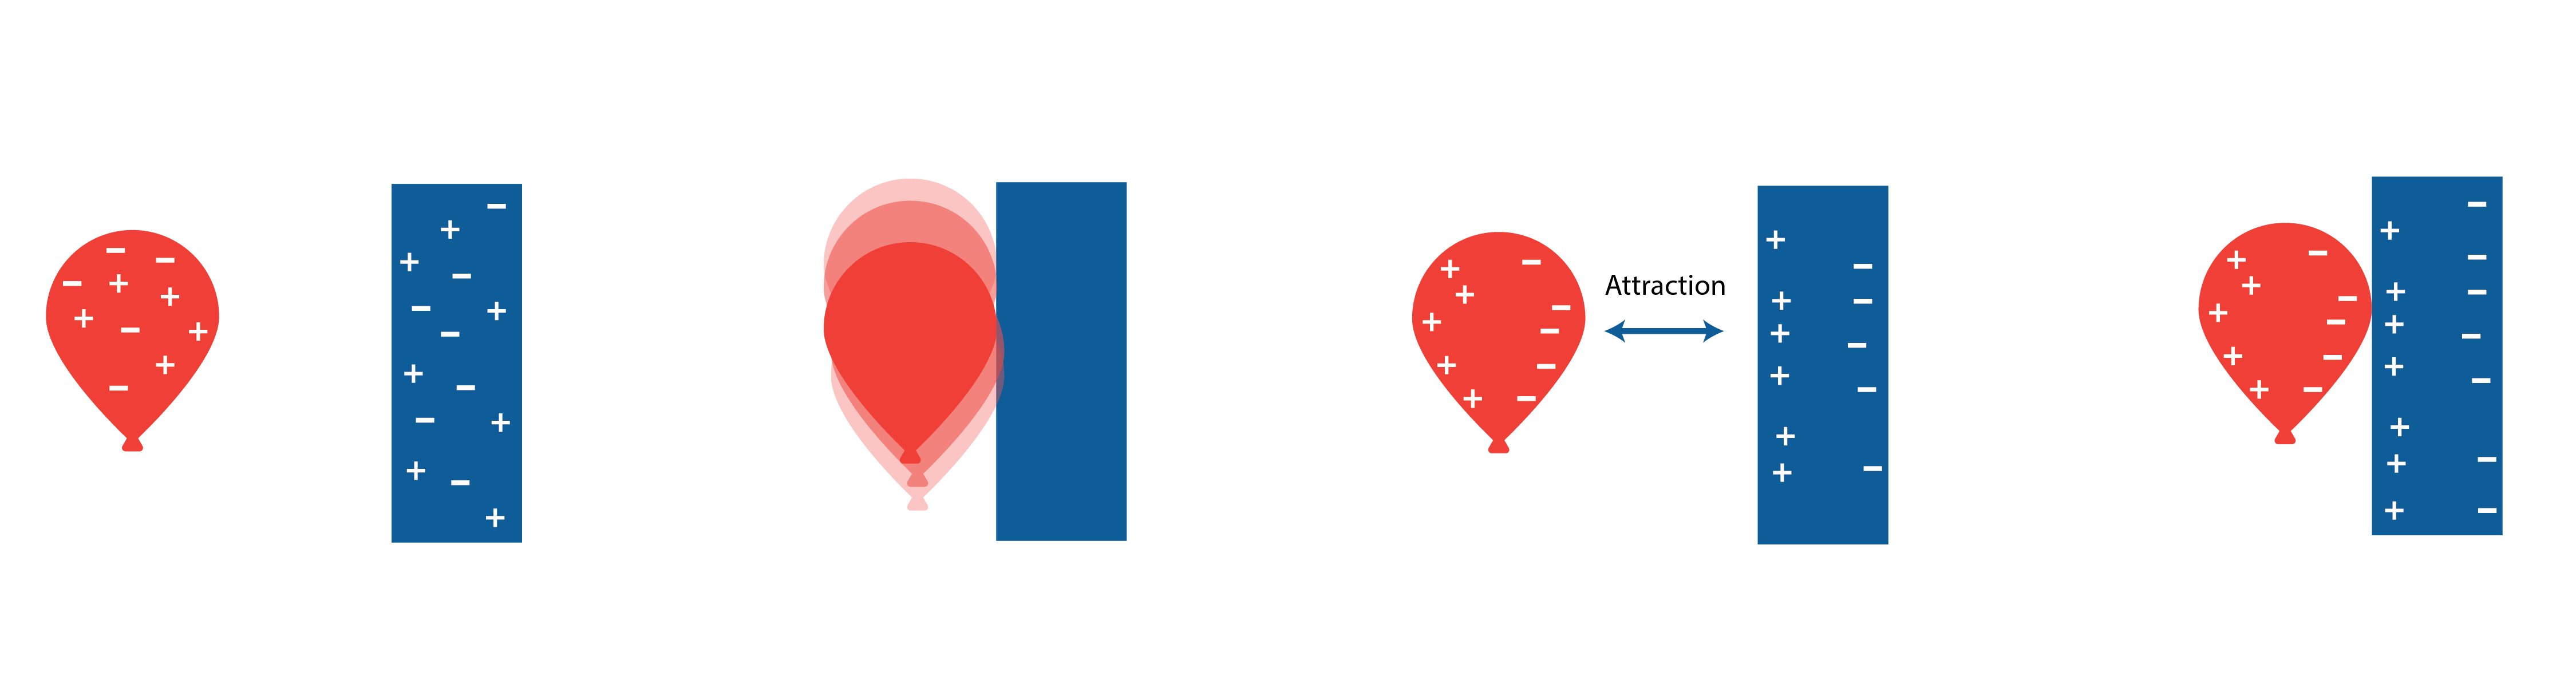
\includegraphics[width=1\textwidth]{balloon2.png}

\section{Lightning}

A cloud is a cluster of water droplets and ice particles. These
droplets and ice particles are always moving up and down through the
cloud. In this process, electrons get stripped off and end up on the
water droplets at the bottom of the cloud (water droplets collect at the bottom because they are denser). The air between the
droplets is a pretty good insulator, which means the electrons are reluctant
to jump anywhere. However, eventually, the charge gets so strong that
even the insulating properties of the air is not enough to prevent
the jump, causing lightning.
% ADD: Add water density explanation. ice less dense than liquid water due to crystaline structure.

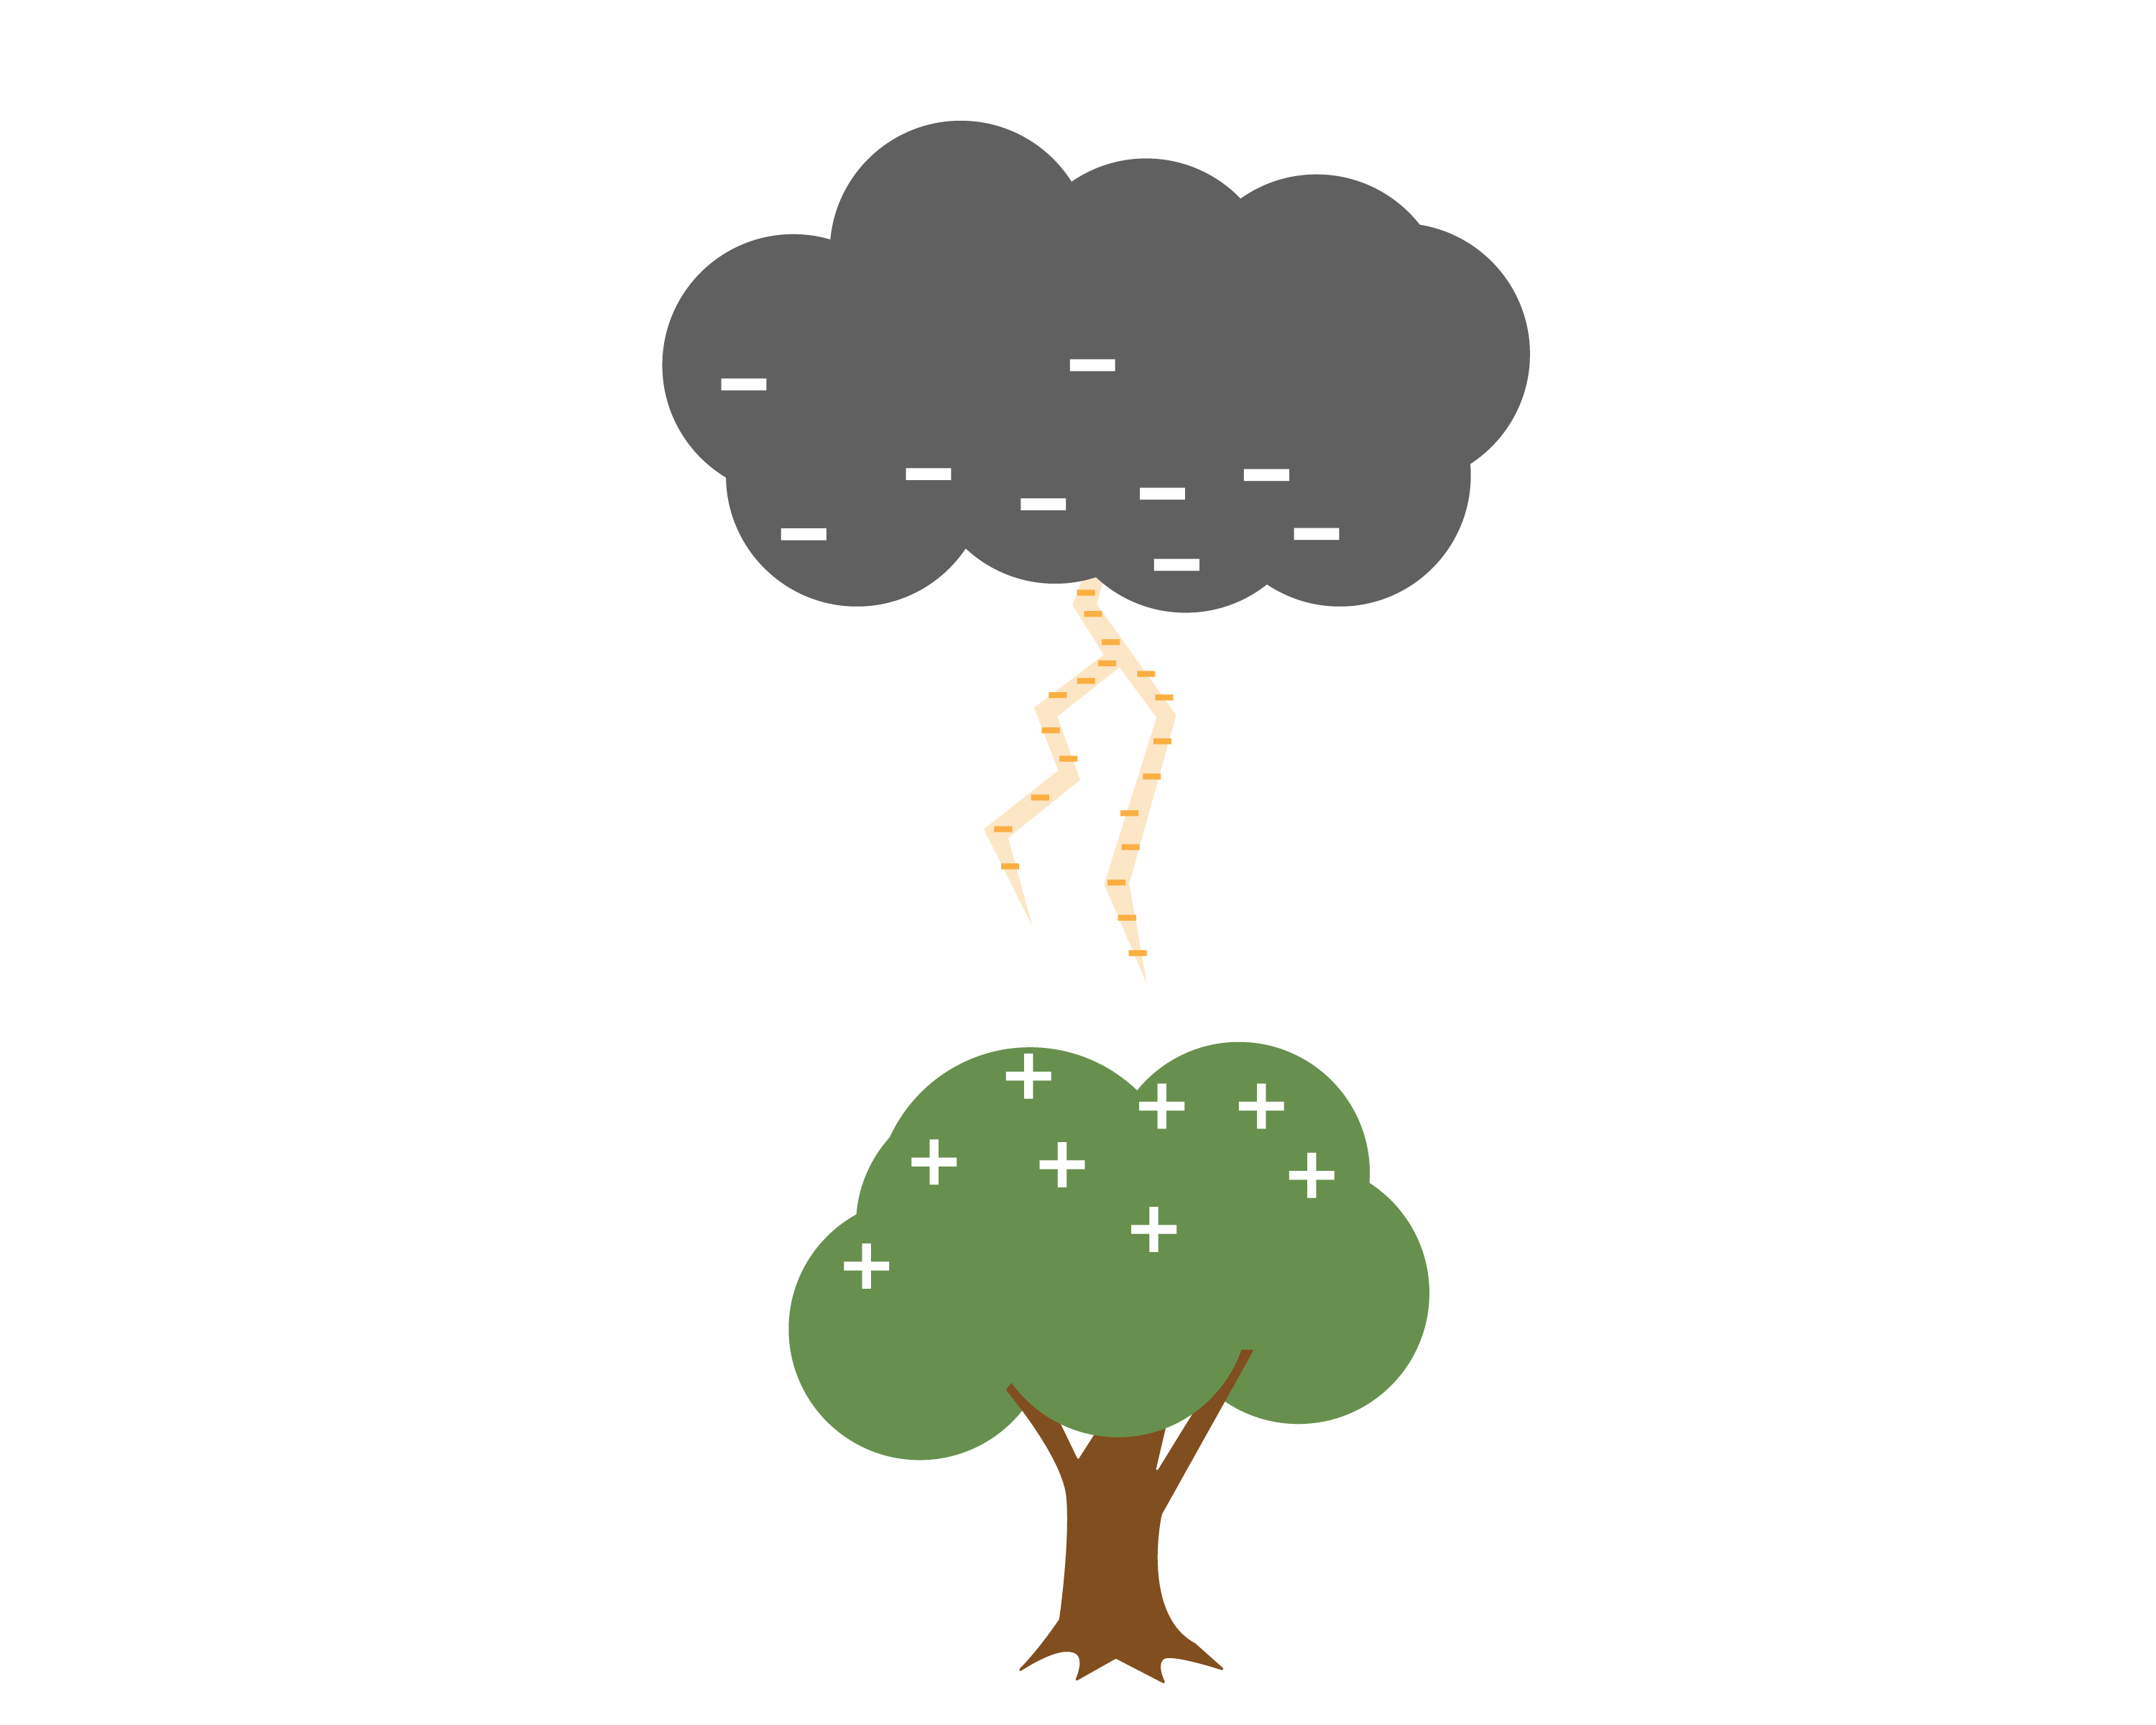
\includegraphics[width=1\textwidth]{lightning.png}

A great deal of lightning moves within a cloud or between clouds. However, sometimes it jumps to the earth. These bolts of lightning vary in the amount of
electrons they carry, but the average is about 15 coulombs.

Thunder occurs because the electrons heat the air they pass through, 
causing the air to expand suddenly. Tthe resulting shockwave is the sound we know as thunder.
% ADD: Relate speed of light and sound 
\section{But...}

This idea that opposite charges attract creates some heavy questions
that you do not yet have the tools to work with. So to these questions, the answer is
basically ``Don't ask that yet!''

However, you probably have these questions, so we will point you in
the direction of the answers.

The first is ``In any atom bigger than hydrogen, there are multiple
protons in the nucleus. Why don't the protons push each other out of
the nucleus?''

We aren't ready to talk about it, but there is a force called \textit{the
 nuclear force}, which pulls the protons and neutrons in the nucleus
of the atom toward each other. At very, very small distances, it is
strong enough to overpower the repulsive force due to the protons'
charges.
% ADD: Effective nuclear charge

Another question is ``Why do the electrons whiz around in a cloud so
far from the nucleus of the atom? Negatively charged electrons should
cling to the protons in the center, right?''

We aren't ready to talk about this either, but quantum mechanics tells us that
electrons like to live in a certain specific energy level. Hugging
protons isn't one of those levels.


\graphicspath{{../../Chapters/volume_solids/en_US}}
\chapter{Volumes of Common Solids}
\section{Rectangular Prism}
The volume of a rectangular solid is the product of its three
dimensions. If a block of ice is 5 cm tall, 3 cm wide, and 2 cm
deep, its volume is $5 \times 3 \times 2 = 30$ cubic centimeters.

\begin{mdframed}[style=important, frametitle={Volume of a rectangular solid.}]

A rectangular solid with height $h$, width $w$ and length/depth $l$ has volume:
$$V = lwh$$
\end{mdframed}

\tdplotsetmaincoords{80}{130} 
\begin{tikzpicture} [scale=1, tdplot_main_coords, axis/.style={->,sdkblue}, 
light vector/.style={-stealth,dashed,very thick, black}, 
vector/.style={-stealth,black,very thick}, 
vector guide/.style={dashed,sdkblue}]

%standard tikz coordinate definition using x, y, z coords
\coordinate (O) at (0,0,0);

%draw axes
\draw[axis] (0,0,0) -- (3,0,0) node[anchor=north east]{$x$};
\draw[axis] (0,0,0) -- (0,4,0) node[anchor=north west]{$y$};
\draw[axis] (0,0,0) -- (0,0,5.2) node[anchor=south]{$z$};

%draw a vector from O to P
\draw[thick,black] (0,0,0) -- (0,0,5);
\draw[thick,black] (0,3,5) -- (0,0,5);
\draw[thick,black] (2,0,5) -- (0,0,5);

\draw[thick,black] (0,0,0) -- (0,3,0);
\draw[thick,black] (0,3,5) -- (0,3,0) node[midway, right]{$5$ cm};
\draw[thick,black] (2,3,0) -- (0,3,0) node[midway, below]{$2$ cm};;

\draw[thick,black] (0,0,0) -- (2,0,0);
\draw[thick,black] (2,0,5) -- (2,0,0);
\draw[thick,black] (2,3,0) -- (2,0,0) node[midway,below]{$3$ cm};

\draw[thick,black] (2,3,5) -- (2,0,5);
\draw[thick,black] (2,3,5) -- (0,3,5);
\draw[thick,black] (2,3,5) -- (2,3,0);

\end{tikzpicture}


A
cubic centimeter is the same as a milliliter. A milliliter of ice
weighs about 0.92 grams.  This means the block of ice would have a mass of $30
\times 0.92 = 27.6$ grams. \index{volume ! rectangular solid}
\section{Triangular Prism}\index{volume ! triangular prism}
Triangular prisms are 3D versions of triangles (imagine stretching a triangle out of the page). 
It has 2 triangular faces and 3 rectangular faces.
\begin{mdframed}[style=important, frametitle={Volume of a triangular prism.}]
Recall the area of a triangle is $V=\frac{1}{2}wh$ where w is the width or base and h is the height of the triangle.
A triangular prism with height $h$, width $w$ and length/depth $l$ has volume:
$$V = \frac{1}{2}lwh$$
\end{mdframed}

%FIXME image is basic, match with other format
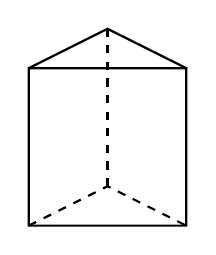
\begin{tikzpicture}
 \draw[dashed,thick] (-1,0) -- (0,0.5) edge (0,2.5) -- (1,0);
 \draw[thick] (-1,0) rectangle (1,2) -- (0,2.5) -- (-1,2);
\end{tikzpicture}

\section{Spheres}
\begin{mdframed}[style=important, frametitle={Volume of a Sphere}]

A sphere with a radius of $r$ has a volume of \index{volume ! sphere}

$$v = \frac{4}{3} \pi r^3$$

(For completeness, the surface area of that sphere would be

$$a  = 4 \pi r^2$$

Note that a circle of radius $r$ is one quarter of this: $\pi r^2$.)

\end{mdframed}

\begin{Exercise}[title={Flying Sphere}, label=flying_sphere]

An iron sphere is traveling at 5 m/s (and is not spinning).  The
sphere has a radius of 1.5 m.  Iron has a density of 7,800 kg per
cubic meter.  How much kinetic energy does the sphere have?
\end{Exercise}
\begin{Answer}[ref=flying_sphere]
  The volume of the sphere (in cubic meters) is

  $$\frac{4}{3}\pi (1.5)^3 = 4.5 \pi \approx 14.14$$

  The mass (in kg) is $14.14 \times 7800 \approx 110,269$

  The kinetic energy (in joules) is

  $$k = \frac{110269 \times 5^2}{2} = 1,378,373$$

  About 1.4 million joules.
\end{Answer}

\section{Cylinders}

The base and the top of a right cylinder are identical circles. The
circles are on parallel planes.  The sides are perpendicular to those
planes.

\tdplotsetmaincoords{75}{0} 
\begin{tikzpicture} [scale=4, tdplot_main_coords, axis/.style={->,sdkblue}]
\draw[dashed, sdkblue] (0.5,0,0) -- (0.5,0,0.7) node[midway, right]{$h$};
\draw[dashed, sdkblue] (0.5,0,0) -- (1,0,0) node[midway, below]{$r$};
\draw[black] (0.5, 0, 0) circle (0.5);
\draw[black] (0.5, 0, 0.7) circle (0.5);
\draw[black] (0,0,0) -- (0,0,0.7);
\draw[black] (1,0,0) -- (1,0,0.7);
\draw[black] (0.5,0,0) circle (0.02);
\draw[black] (0.5,0,0.7) circle (0.02);
\end{tikzpicture}

\begin{mdframed}[style=important, frametitle={Volume of a cylinder}]\index{volume ! right cylinder}


The volume of the right cylinder of radius $r$ and height
$h$ is given by:

$$v = \pi r^2 h$$

In other words, it is the area of the base times the height.

\end{mdframed}

\begin{Exercise}[title={Tablet}, label=tablet]

  A drug company needs to create a tablet with volume of 90 cubic millimeters.

  The tablet will be a cylinder with half spheres on each end.  The radius will be 2mm.

  How long do they need to make the tablet to be?

  \vspace{2mm}
  
\tdplotsetmaincoords{90}{20} 
\begin{tikzpicture} [scale=6.5, tdplot_main_coords, axis/.style={->,sdkblue}]
\draw[dashed, sdkblue] (-0.2,0,0) -- (0,0,0);
\draw[dashed, sdkblue] (0,0,0) -- (0,0,0.2) node[midway, right]{2 mm};
\draw[dashed, sdkblue] (0, 0, 0) [x={(0,0,1)}] circle (0.2);
\draw[dashed, sdkblue] (0.5, 0, 0) [x={(0,0,1)}] circle (0.2);
\draw[dashed, sdkblue] (0.5,0,0) -- (0.7,0,0);
\draw[black] (0, 0, -0.2) [y={(0,0,-1)}] arc (90:270:0.2);
\draw[black] (0.5, 0, 0.2) [y={(0,0,-1)}] arc (-90:90:0.2);
\draw[black] (0,0,0.2) -- (0.5,0,0.2);
\draw[black] (0,0,-0.2) -- (0.5,0,-0.2);
\draw[dashed, sdkblue] (-0.2, 0, 0) -- (-0.2, 0, -0.3);
\draw[dashed, sdkblue] (0.7, 0, 0) -- (0.7, 0, -0.3);
\draw[dashed, sdkblue] (-0.2, 0, -0.3) -- (0.7, 0, -0.3) node[midway, below]{?};
\end{tikzpicture}
  

\end{Exercise}
\begin{Answer}[ref=tablet]
  In your mind, you can disassemble the tablet into a sphere (made up of
  the two ends) and a cylinder (between the two ends).
  
  The volume of the sphere (in cubic millimeters) is

  $$\frac{4}{3}\pi (2)^3 =\frac{32}{3}\pi \approx 33.5$$

  Thus, the cylinder part has to be $90 - 33.5 = 56.5$ cubic mm. The
  cylinder part has a radius of 2 mm. If the length of the cylinder
  part is $x$, then

  $$\pi 2^2 x = 56.5$$

  Thus $x = \frac{56.5}{4 \pi} \approx 4.5$ mm.

  The cylinder part of the table needs to be 4.5mm.  Thus the entire tablet is 8.5mm long.
  
\end{Answer}

What if the base and top are identical, but the sides aren't
perpendicular to the base? This is called \newterm{oblique cylinder}.

\tdplotsetmaincoords{75}{0} 
\begin{tikzpicture} [scale=4, tdplot_main_coords, axis/.style={->,sdkblue}]
\draw[dashed, sdkblue] (0.7,0,0) -- (0.7,0,0.7) node[midway, right]{$h$};
\draw[dashed, sdkblue] (0.5,0,0) -- (1,0,0) node[midway, below]{$r$};
\draw[black] (0.5, 0, 0) circle (0.5);
\draw[black] (0.7, 0, 0.7) circle (0.5);
\draw[black] (0,0,0) -- (0.2,0,0.7);
\draw[black] (1,0,0) -- (1.2,0,0.7);
\draw[black] (0.5,0,0) circle (0.02);
\draw[black] (0.7,0,0.7) circle (0.02);
\end{tikzpicture}

The volume is still the height times the area of the base.  Note,
however, that the height is measured perpendicular to the bottom and
top. \index{volume ! oblique cylinder}

Why is this the case?


\section{Pyramids}

On a solid with a flat base, the line that we use to measure height is
always perpendicular to the plane of the base. We can take slices
through the solid that are parallel to that base plane.  For example,
if we have a pyramid with a square base, each slice will be a square
--- small squares near the top, larger squares near the bottom. 
The sides of the pyramids are all triangles, so these are referred to as Triangular Pyramids, just pyramids, or sometimes, Tetrahedrons.
\tdplotsetmaincoords{80}{17} 
\begin{tikzpicture} [scale=4, tdplot_main_coords, axis/.style={->,sdkblue}]
  
\draw[dashed, sdkblue] (0.5,0.5,0) -- (0.5,0.5, 1.0) node[midway, right]{$h$};

\draw[black] (0,0,0) -- (0.5,0.5,1.0);
\draw[black] (1,0,0) -- (0.5,0.5,1.0);
\draw[black] (0,1,0) -- (0.5,0.5,1.0);
\draw[black] (1,1,0) -- (0.5,0.5,1.0);

\draw[black] (0,0,0) -- (1,0,0);
\draw[black] (0,0,0) -- (0,1,0);
\draw[black] (1,0,0) -- (1,1,0)node[midway,below]{$w$};
\draw[black] (0,1,0) -- (1,1,0);

\fill[sdkblue,,opacity=0.4] (0.125, 0.125, 0.25) -- (0.875, 0.125, 0.25) -- (0.875, 0.875, 0.25) -- (0.125, 0.875, 0.25);

\draw[dashed,sdkblue] (0.125, 0.125, 0.25) -- (0.875, 0.125, 0.25);
\draw[dashed,sdkblue] (0.125, 0.125, 0.25) -- (0.125, 0.875, 0.25);
\draw[dashed,sdkblue] (0.875, 0.125, 0.25) -- (0.875, 0.875, 0.25);
\draw[dashed,sdkblue] (0.125, 0.875, 0.25) -- (0.875, 0.875, 0.25);

\draw[dashed,sdkblue] (-0.1, -0.1, 0.25) -- (1.1, -0.1, 0.25);
\draw[dashed,sdkblue] (-0.1, -0.1, 0.25) -- (-0.1, 1.1, 0.25);
\draw[dashed,sdkblue] (1.1, -0.1, 0.25) -- (1.1, 1.1, 0.25);
\draw[dashed,sdkblue] (-0.1, 1.1, 0.25) -- (1.1, 1.1, 0.25);

\end{tikzpicture}

We can figure out the area of the slice at every height $z$.  For
example, at $z = 0$, the slice would have area $w^2$.  At $z = h$, the
slice would have zero area.  What about an arbitrary $z$ in between?
The edge of the square would be $w (1 - \frac{z}{h})$.  The area of
the slice would be $w^2 (1 - \frac{z}{h})^2$

The graph of this would look like this:

\begin{tikzpicture}[scale=5]

\draw [sdkblue,->,thick] (0,0) -- (1.1,0) node[right]{$z$};
\draw [sdkblue,->,thick] (0,0) -- (0,1.1) node[above]{slice area};
\draw [sdkblue,dashed] (1, 1) -- (0,1) node[left] {$w^2$};
\draw [sdkblue,dashed] (1, 1) -- (1,0) node[below] {$h$};
 \fill [sdkblue, opacity=0.4, domain=0:1, variable=\x]
      (0, 0) 
      -- plot ({\x}, {(1.0 - \x)^2})
      -- (1, 0)
      -- cycle;
\draw[thick,draw=black,
      domain=0:1,samples=300,variable=\x] 
      plot (\x,{(1.0 - \x)^2});
\end{tikzpicture}

The volume is given by the area under the curve and above the
axis. Once you learn integration, you will be extra good at finding
the area under the curve.  In this case, we will just tell you that the colored region in the picture is one third of the rectangle.

Thus, the area of a square-based pyramid is $\frac{1}{3} h w^2$.

In fact:

\begin{mdframed}[style=important, frametitle={Volume of a pyramid}]\index{volume ! pyramid}

  The volume of pyramid whose base has an area of $b$ and height $h$ is given by:

  $$V = \frac{1}{3} h b$$

  Regardless of the shape of the base.
\end{mdframed}

Note that this is true even for oblique pyramids:

\tdplotsetmaincoords{80}{30} 
\begin{tikzpicture} [scale=4, tdplot_main_coords, axis/.style={->,sdkblue}]
  
\draw[dashed, sdkblue] (1.6,0.5,0) -- (1.6,0.5, 1.0) node[midway, right]{$h$};
\fill[sdkblue] (1.6, 0.5, 0) circle (.02);

\draw[black] (0,0,0) -- (1.6,0.5,1.0);
\draw[black] (1,0,0) -- (1.6,0.5,1.0);
\draw[black] (0,1,0) -- (1.6,0.5,1.0);
\draw[black] (1,1,0) -- (1.6,0.5,1.0);

\draw[black] (0,0,0) -- (1,0,0);
\draw[black] (0,0,0) -- (0,1,0);
\draw[black] (1,0,0) -- (1,1,0);
\draw[black] (0,1,0) -- (1,1,0);

\fill[sdkblue,opacity=0.4] (0.4, 0.125, 0.25) -- (1.15, 0.125, 0.25) -- (1.15, 0.875, 0.25) -- (0.4, 0.875, 0.25);

\draw[dashed,sdkblue] (0, -0.1, 0.25) -- (1.3, -0.1, 0.25);
\draw[dashed,sdkblue] (0, -0.1, 0.25) -- (0, 1.1, 0.25);
\draw[dashed,sdkblue] (1.3, -0.1, 0.25) -- (1.3, 1.1, 0.25);
\draw[dashed,sdkblue] (0, 1.1, 0.25) -- (1.3, 1.1, 0.25);

\end{tikzpicture}


\begin{Exercise}[title={Hexagon-based Pyramid}, label=pyramid_volume]

There is a pyramid with a regular hexagon for a base. Each edge is 5 cm long.  The pyramid is 13 cm tall.  What is its volume?

\tdplotsetmaincoords{70}{17} 
\begin{tikzpicture} [scale=.5, tdplot_main_coords]
  
\draw[dashed, sdkblue] (0,0,0) -- (0,0,13) node[right]{13 cm};

\draw[black] (-5,0,0) -- (-2.5,4.33,0) -- (2.5,4.33,0) -- (5,0,0)
-- (2.5, -4.33, 0) -- (-2.5, -4.33,0) -- cycle;

\draw[black] (0, -4.5, 0) node {5 cm};

\draw[black] (-5,0,0) -- (0,0,13);
\draw[black] (0,0,13)--(5,0,0);
\draw[black] (-2.5,4.33,0) -- (0,0,13);
\draw[black] (2.5,4.33,0) -- (0,0,13);
\draw[black] (-2.5,-4.33,0) -- (0,0,13);
\draw[black] (2.5,-4.33,0) -- (0,0,13);
\end{tikzpicture}

\end{Exercise}
\begin{Answer}[ref=pyramid_volume]
  First, you need to find the area of the base, which is a regular hexagon:
  
\begin{tikzpicture}[scale=0.5]
  \draw[black] (-5,0) -- (-2.5,4.33) -- (2.5,4.33) -- (5,0)
-- (2.5, -4.33) -- (-2.5, -4.33) -- cycle node[midway,left]{5 cm};
\draw[sdkblue,dashed] (-5,0) -- (0,0);
\draw[sdkblue,dashed] (5,0) -- (0,0);
\draw[sdkblue,dashed] (-2.5,4.33) -- (0,0);
\draw[sdkblue,dashed] (2.5,4.33) -- (0,0);
\draw[sdkblue,dashed] (-2.5,-4.33) -- (0,0);
\draw[sdkblue,dashed] (2.5,-4.33) -- (0,0);
\end{tikzpicture}

All the angles in this picture are $60^\circ$ or $\frac{\pi}{3}$
radians. This means each line is 5 cm long.

This tells us that we need to find the area of one of these triangles and multiply that by six.

Every triangle has a base of 5cm. How tall are they?

\begin{tikzpicture}
  \draw[black] (-2.5,0) -- (2.5,0) -- (0,4.33) -- cycle node[midway,left]{5 cm};
  \draw[sdkblue,dashed] (0,0) -- (0,4.33) node[midway,right]{?};
  \draw[black] (-2.0, 0.0) node [right, above] {$60^\circ$};
\end{tikzpicture}

$$5 \sin{60^\circ} = 5\frac{\sqrt{3}}{2}$$

Which is about 4.33 cm.

So, the area of single triangle is 

$$\frac{1}{2} (5) \left( 5\frac{\sqrt{3}}{2} \right) = 25 \frac{\sqrt{3}} {4}$$

And the area of the whole hexagon is six times that:

$$75 \frac{\sqrt{3}}{2}$$

Thus, the volume of the pyramid is:

$$\frac{1}{3}h b = \frac{1}{3} 13 \left(75 \frac{\sqrt{3}}{2}\right)$$

About 281.46 cubic centimeters.

\end{Answer}

Note that plotting the area of each slice and finding the area under
the curve will let you find the area of many things.  For example,
let's say that you have a four-sided spiral, where each face has the
same width $w$:

\tdplotsetmaincoords{80}{17} 
\begin{tikzpicture} [scale=4, tdplot_main_coords, axis/.style={->,sdkblue}]

  \def\h{1.570796326794897}
  \def\gap{0.2}
  \def\srad{0.707106781186548}

\fill[sdkblue,opacity=.7] (0,-1,0) -- (-1,0,0) -- (0,1,0) -- (1,0,0) -- cycle;

\draw[black,thick] (0,-1,0) -- (-1,0,0) -- (0,1,0) -- (1,0,0) -- cycle;
\draw[black,thick] (0,-1,\h) -- (-1,0,\h) -- (0,1,\h) -- (1,0,\h) -- cycle;

\foreach \x in {0.0, 0.1, 0.2, 0.3, 0.4, 0.5, 0.6, 0.7, 0.8, 0.9, 1.0, 1.1, 1.2, 1.3, 1.4, 1.5}{
%        \fill[sdkblue, opacity=0.3] ({sin(deg(\x) + 0)},{cos(deg(\x)+ 0)},\x) -- ({sin(deg(\x) + 90)},{cos(deg(\x)+ 90)},\x) --
%        ({sin(deg(\x + \gap) + 90)},{cos(deg(\x + \gap) + 90)},\x + \gap) -- ({sin(deg(\x + \gap) + 0},{cos(deg(\x + \gap)+ 0)},\x + \gap) -- cycle;
        
%        \fill[gray, opacity=0.8] ({sin(deg(\x) + 90)},{cos(deg(\x)+ 90)},\x) -- ({sin(deg(\x) + 180)},{cos(deg(\x)+ 180)},\x) --
%        ({sin(deg(\x + \gap) + 180)},{cos(deg(\x + \gap)+ 180)},\x + \gap) -- ({sin(deg(\x + \gap) + 90)},{cos(deg(\x + \gap)+ 90)},\x + \gap) -- cycle;
        
%        \fill[sdkblue,opacity=0.3] ({sin(deg(\x) + 180)},{cos(deg(\x)+ 180)},\x) -- ({sin(deg(\x) + 270)},{cos(deg(\x)+ 270)},\x) --
%        ({sin(deg(\x + \gap) + 270)},{cos(deg(\x + \gap)+ 270)},\x+\gap) -- ({sin(deg(\x + \gap) + 180)},{cos(deg(\x + \gap)+ 180)},\x + \gap) -- cycle;
        
%        \fill[gray] ({sin(deg(\x) + 270)},{cos(deg(\x)+ 270)},\x) -- ({sin(deg(\x) + 0)},{cos(deg(\x)+ 0)},\x) --
  %        ({sin(deg(\x + \gap) + 0)},{cos(deg(\x + \gap)+0)},\x + \gap) -- ({sin(deg(\x + \gap) + 270)},{cos(deg(\x + \gap)+ 270)},\x +\gap) -- cycle;

  \draw[sdkblue] ({sin(deg(\x) + 0)},{cos(deg(\x)+ 0)},\x) -- ({sin(deg(\x) + 90)},{cos(deg(\x)+ 90)},\x) --
  ({sin(deg(\x) + 180)},{cos(deg(\x)+ 180)},\x) -- ({sin(deg(\x) + 270)},{cos(deg(\x)+ 270)},\x);
      }

\draw[thick,draw=black,
      domain=0:\h,samples=100,variable=\x] 
      plot ({sin(deg(\x) + 0)},{cos(deg(\x)+ 0)}, \x);

\draw[dashed,draw=sdkblue,
      domain=0:\h,samples=100,variable=\x] 
      plot ({\srad * sin(deg(\x) + 45)},{\srad * cos(deg(\x)+ 45)}, \x);

\draw[thick,draw=black,
      domain=0:\h,samples=100,variable=\x] 
      plot ({sin(deg(\x) + 90)},{cos(deg(\x)+ 90)}, \x);
\draw[dashed,draw=sdkblue,
      domain=0:\h,samples=100,variable=\x] 
      plot ({\srad * sin(deg(\x) + 135)},{\srad * cos(deg(\x)+ 135)}, \x);
      
\draw[thick,draw=black,
      domain=0:\h,samples=100,variable=\x] 
      plot ({sin(deg(\x) + 180)},{cos(deg(\x) + 180)}, \x);
%\draw[dashed,draw=sdkblue,
%      domain=0:\h,samples=100,variable=\x] 
%      plot ({\srad * sin(deg(\x) + 225)},{\srad * cos(deg(\x)+ 225)}, \x);

      
\draw[dashed, thick,draw=black,
      domain=0:\h,samples=100,variable=\x] 
      plot ({sin(deg(\x) + 270)},{cos(deg(\x) + 270)}, \x);

%\draw[dashed,draw=sdkblue,
%      domain=0:\h,samples=100,variable=\x] 
%      plot ({\srad * sin(deg(\x) + 315)},{\srad * cos(deg(\x)+ 315)}, \x);


      \fill[sdkblue,opacity=.9] (0,-1,\h) -- (-1,0,\h) -- (0,1,\h) -- (1,0,\h) -- cycle;
      \draw (0.7,-0.6,0) node [below] {$w$};
      \draw[dashed, sdkblue] (-1.1,0,0) -- (-1.1,0,\h) node[midway,left]{$h$};


\end{tikzpicture}

Every slice still has an area of $w^2$,  which means this figure has a volume of $h w^2$.


\begin{Exercise}[title={Volume of a building}, label=building_volume]

An architect is designing a hotel with a right triangular base; the base is 30
meters on each leg.  The building gets narrower as you get closer to
the top, and finally shrinks to a point.  The spine of the building is
where the right angle is. That spine is straight and perpendicular to the ground.

Each floor has a right isosceles triangle as its floor plan.  The
length of each leg is given by this formula:

$$w = 30 \sqrt{1 - \frac{z}{100}}$$

So, the width of the building is 30 meters at height $z=0$.  At 100
meters, the building comes to a point.  It will look like this:
\hspace{8mm}

\tdplotsetmaincoords{75}{120}
\begin{tikzpicture} [scale=1, tdplot_main_coords]
\def\h{10}
\draw[dashed, sdkblue] (0,3,0) -- (0,3.2,0) -- (0,3.2,\h) node[midway, right]{100m} -- (0,0,\h);

\draw[black] (0,0,0) -- (3,0,0) -- (0,3,0) -- cycle node [midway, above]{30m};
\draw[black] (0,0,0) -- (0,0,\h);
\draw[black] (0.5, 0, 0) -- (0.5, 0.5, 0) -- (0, 0.5, 0);
\draw[thick,draw=black,
      domain=0:\h,samples=100,variable=\x] 
      plot ({3 * sqrt(1 - (\x/\h)}, 0, \x);

\draw[thick,draw=black,
      domain=0:\h,samples=100,variable=\x] 
      plot (0, {3 * sqrt(1 - (\x/\h))}, \x);

\foreach \n in {1,...,\h}{
  \draw [dashed, draw=sdkblue] (0,0,\n) -- ({3 * sqrt(1 - \n/\h)}, 0, \n) -- (0, {3 * sqrt(1 - \n/\h)},\n) -- cycle;
  \draw [draw=sdkblue] (0.5,0,\n) -- (0.5, 0.5, \n) -- (0, 0.5,\n);
};
      
\end{tikzpicture}

What is the volume of the building in cubic meters?
\end{Exercise}
\begin{Answer}[ref=building_volume]

  The area at height $z$ is given by:

  $$a = \frac{1}{2} w^2 =\frac{1}{2} \left(30 \sqrt{1 - \frac{z}{100}}\right)^2 = \frac{1}{2} 900 \left(1 - \frac{z}{100}\right)$$

  If we plot that, it looks like this:

\begin{tikzpicture}
  \def\h{5}
  \draw[sdkblue, ->] (0,0) -- (0, \h + 0.5) node[above] {area};
  \draw[sdkblue, ->] (0,0) -- (3.5, 0) node[right] {$z$};
 \fill [sdkblue, opacity=0.4]
      (0, 0) -- (0,\h) node [left] {$900 m^2$} -- (3,0) node[below] {$100 m$} -- cycle;
\end{tikzpicture}

What is the area of the blue region? $\frac{1}{2} (900)(100) = 45,000$

The building will be 45 thousand cubic meters.


\end{Answer}
% FIXME
% volume of ellipse? 
% and cone since it is included in quiz questions and heavily in the next chapter
\graphicspath{{../../Chapters/angles/en_US}}
\chapter{Angles}

In the following recommend videos, the narrator talks about
lines, line segments, and rays. When mathematicians talk about
\emph{lines}\index{lines}, they mean a straight line that goes forever in two 
directions. And if you pick any two points on that line; the space between 
them is a \emph{line segment}\index{line segment}. If you take any line, pick 
a point on that line and discard all the points on one side of the point, that 
is a \emph{ray}\index{ray}. All three have no width.

\begin{center}
\begin{tikzpicture}[scale=1.5]
  \coordinate (a) at (-0.3, -0.6);
  \coordinate (d) at (1.3, 2.6);
  \draw [<->](a)--node [right]{"Line"}(d);
\end{tikzpicture}
\hspace{10mm}
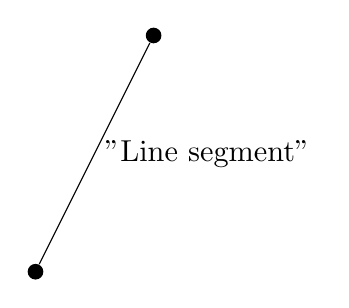
\begin{tikzpicture}[scale=1.5]
  \coordinate [circle, fill, inner sep=2pt] (b) at (0,0) ;
  \coordinate [circle, fill, inner sep=2pt] (c) at (1, 2) ;
  \draw (b)--node [right]{"Line segment"}(c);
\end{tikzpicture}
\hspace{6mm}
\begin{tikzpicture}[scale=1.5]
  \coordinate [circle, fill, inner sep=2pt] (b) at (0,0) ;
  \coordinate (d) at (1.3, 2.6);
  \coordinate (lab) at (0.8, 1.0);
  \draw [->](b)--node[right] {"Ray"} (d)  ;
\end{tikzpicture}
\end{center}



Watch the following videos from Khan Academy:
\begin{itemize}
\item Introduction to angles: \url{https://youtu.be/H-de6Tkxej8}
\item Measuring angles in degrees: \url{https://youtu.be/92aLiyeQj0w} 
\end{itemize}

When two lines cross, they form four angles:

\begin{center}
\begin{tikzpicture}[scale=3]
  \coordinate (a) at (0, 1.5);
  \coordinate (b) at (1.6, 2);
  \coordinate (c) at (1.6, 1.5);
  \coordinate (d) at (0, 1);
  \coordinate [circle, fill, inner sep=1pt](e) at (0.8, 1.5) ;
  \draw [->](e)--(a) node[left] {$A$}  ;
  \draw [->](e)--(b) node[right] {$B$}  ;
  \draw [->](e)--(c) node[right] {$C$}  ;
  \draw [->](e)node[above]{$E$}--(d) node[left] {D} ;
  \pic [draw, <->, "$\scriptstyle  \angle AEB$ ", angle radius = 0.8cm, 
  angle eccentricity=1.3] {angle = b--e--a};
  \pic [draw, <->, "$\scriptstyle  \angle BEC$ ", angle radius = 1.1cm, 
  angle eccentricity = 1.5] {angle = c--e--b};
  \pic [draw, <->, "$\scriptstyle  \angle CED$ ", angle radius = 0.8cm, 
  angle eccentricity=1.3] {angle = d--e--c};
  \pic [draw, <->, "$\scriptstyle  \angle DEA$ ", angle radius = 1.1cm, 
  angle eccentricity=1.5] {angle = a--e--d};
\end{tikzpicture}
\end{center}


What do we know about those angles?
\begin{itemize}
\item The sum of any two adjacent angles add to be $180^\circ$.  So, for 
example, $m \angle AEB + m \angle BEC = 180^\circ$. We use the phrase ``add to 
be $180^{\circ}$'' so often that we have a special word for it: 
\emph{supplementary}.\index{supplementary angles}
\item The sum of all four angles is $360^\circ$.
\item Angles opposite each other are equal. So, for example, $m \angle AEB = m 
\angle CED$.
\end{itemize}

In a diagram, to indicate that two angles are equal we often put hash marks in 
the angle:

\begin{center}
\begin{tikzpicture}[scale=3]
  \coordinate (a) at (0, 1.5);
  \coordinate (b) at (1.6, 2);
  \coordinate (c) at (1.6, 1.5);
  \coordinate (d) at (0, 1);
  \coordinate [circle, fill, inner sep=1pt](e) at (0.8, 1.5) ;
  \draw [->](e)--(a) node[left] {$A$}  ;
  \draw [->](e)--(b) node[right] {$B$}  ;
  \draw [->](e)--(c) node[right] {$C$}  ;
  \draw [->](e)node[above]{$E$}--(d) node[left] {D} ;
  \tkzMarkAngle[size = 0.2cm,mark = |](b,e,a)
  \tkzMarkAngle[size = 0.3cm,mark = ||](c,e,b)
  \tkzMarkAngle[size = 0.2cm,mark = |](d,e,c)
  \tkzMarkAngle[size = 0.3cm,mark = ||](a,e,d)
\end{tikzpicture}
\end{center}


Here the two angles with a single hash mark are equal and the two angles with 
double hash marks are equal.

When two lines are perpendicular, the angle between them is $90^\circ$ and we 
say they meet at a \emph{right angle}. When drawing diagrams, we indicate right
angles with an elbow:

\begin{center}
\begin{tikzpicture}[scale=1.5]
  \coordinate (a) at (0, 1.5);
  \coordinate (b) at (0, 0);
  \coordinate (c) at (1.5, 0);
  \draw [->](b)--(a)  ;
  \draw [->](b)--(c)  ;
  \pic [draw,thick,angle eccentricity=.5]{right angle = a--b--c};
\end{tikzpicture}
\end{center}

 
When an angle is less than $90^\circ$, it is said to be
\emph{acute}. When an angle is more than $90^\circ$, it is said to be
\emph{obtuse}.
% Add: Complementary Angles

\begin{center}
\begin{tikzpicture}[scale=3]
  \coordinate (a) at (0.4, 0.6);
  \coordinate (b) at (0, 0);
  \coordinate (c) at (0.9, 0);
  \draw [->](b)--(a)  ;
  \draw [->](b)--(c)  ;
  \pic [draw, <->, "acute", angle radius = 1cm, angle eccentricity=1.5] {
  angle = c--b--a};
  \end{tikzpicture}
\hspace{2cm}
\begin{tikzpicture}[scale=3]
  \coordinate (a) at (1, 0.6);
  \coordinate (b) at (0.5, 0);
  \coordinate (c) at (0, 0);
  \draw [->](b)--(a)  ;
  \draw [->](b)--(c)  ;
  \pic [draw, <->, "obtuse", angle radius = 0.6cm, angle eccentricity=1.5] {
  angle = a--b--c};
\end{tikzpicture}
\end{center}


If two lines are parallel, line segments that intersect both lines, form the 
same angles with each line:

\begin{center}
\begin{tikzpicture}[scale=3]
  \coordinate (a) at (0, 1);
  \coordinate [circle, fill, inner sep=1pt](b) at (1.5, 1.5);
  \coordinate (c) at (1.5, 1);
  \coordinate (d) at (0.5, 0.5);
  \coordinate (e) at (1, 1);
  \coordinate (f) at (0, 0.5);
  \coordinate (g) at (1.5, 0.5);
  \coordinate [circle, fill, inner sep=1pt](h) at (0, 0);
  \draw [->](e)--(a);
  \draw [-](e)--(b);
  \draw [->](e)--(c);
  \draw [-](e)--(d);
   \draw [->](d)--(f);
  \draw [->](d)--(g);
  \draw [-](d)--(h);
  \tkzMarkAngle[size = 0.15cm,mark = |](b,e,a)
  \tkzMarkAngle[size = 0.2cm,mark = ||](c,e,b)
  \tkzMarkAngle[size = 0.15cm,mark = |](d,e,c)
  \tkzMarkAngle[size = 0.2cm,mark = ||](a,e,d)
  
   \tkzMarkAngle[size = 0.15cm,mark = |](e,d,f)
  \tkzMarkAngle[size = 0.2cm,mark = ||](g,d,e)
  \tkzMarkAngle[size = 0.15cm,mark = |](h,d,g)
  \tkzMarkAngle[size = 0.2cm,mark = ||](f,d,h)
\end{tikzpicture}
\end{center}


\section{Radians}
As you've seen above, angles can be measured in degrees. Just like you can 
measure length in more than one unit (inches, meters, etc.), there is more 
than one unit to measure angles in. Angles can also be measured in \textit{
radians}\index{radians}. Radians are unitless (that is, you don't have to put 
a letter after the number) and there are $\pi$ radians across a straight line. 
This means $180^\circ$ is the same as $\pi$ radians. 

\textbf{Example}: An angle is measured to be $\frac{\pi}{2}$ radians. What is 
the angle in degrees?

\textbf{Solution}: Since we know that $\pi$ radians is the same as $180^\circ$,
we can set up the unit conversion:
$$\frac{\pi}{2} \cdot \frac{180^\circ}{\pi} = 90^o$$

Therefore, a $\frac{\pi}{2}$ angle is $90^\circ$. 

\begin{Exercise}[label = radians]
Convert the following angles from degrees to radians or from radians to degrees. 
\begin{enumerate}
\item $360^\circ$
\item $\frac{\pi}{3}$
\item $225^\circ$
\item $\frac{3\pi}{4}$
\item $30^\circ$
\item $45^\circ$
\end{enumerate}
\end{Exercise}

\begin{Answer}[ref = radians]
\begin{enumerate}
\item $2\pi$
\item $60^\circ$
\item $\frac{5\pi}{4}$
\item $135^\circ$
\item $\frac{\pi}{6}$
\item $\frac{\pi}{4}$
\end{enumerate}
\end{Answer}




\graphicspath{{../../Chapters/triangles_circles/en_US}}
\chapter{Introduction to Triangles}

Connecting any three points with three line segments will get you a
triangle. Here is the triangle $ABC$ which was created by connecting three points $A$, $B$, and $C$:\index{triangle}

\begin{tikzpicture}[scale=1.5]
  \coordinate [circle, fill, inner sep=2pt] (a) at (0,0) ;
  \coordinate [circle, fill, inner sep=2pt] (b) at (1, 2) ;
  \coordinate [circle, fill, inner sep=2pt] (c) at (3,0) ;
  \draw (a)--(b) node [outer sep=3pt, above]{$B$};
  \draw (b)--(c) node[outer sep=3pt, right]{$C$};
  \draw (c)--(a) node[outer sep=3pt, left]{$A$};
\end{tikzpicture}

\section{Equilateral and Isosceles Triangles}
% Add scalene Triaganle
We talk a lot about the length of the sides of triangles. If all three sides of the triangle are the same length, we say it is an \emph{equilateral triangle}:\index{equilateral triangle}

\begin{tikzpicture}[scale=1.5]
  \coordinate [circle, fill, inner sep=2pt] (a) at (0,0) ;
  \coordinate [circle, fill, inner sep=2pt] (b) at (1.5, 2.6) ;
  \coordinate [circle, fill, inner sep=2pt] (c) at (3,0) ;
  \draw (a)--(b) node [outer sep=3pt, above]{$B$};
  \draw (b)--(c) node[outer sep=3pt, right]{$C$};
  \draw (c)--(a) node[outer sep=3pt, left]{$A$};
  \tkzMarkSegment[pos=.5,mark=||](a,b)
  \tkzMarkSegment[pos=.5,mark=||](b,c)
  \tkzMarkSegment[pos=.5,mark=||](c,a)
\end{tikzpicture}

If only two sides of the triangle are the same length, we say it is an \emph{isosceles triangle}:\index{isoscelese triangle}

\begin{tikzpicture}[scale=1.3]
  \coordinate [circle, fill, inner sep=2pt] (a) at (0,0) ;
  \coordinate [circle, fill, inner sep=2pt] (b) at (1.5, 4) ;
  \coordinate [circle, fill, inner sep=2pt] (c) at (3,0) ;
  \draw (a)--(b) node [outer sep=3pt, above]{$B$};
  \draw (b)--(c) node[outer sep=3pt, right]{$C$};
  \draw (c)--(a) node[outer sep=3pt, left]{$A$};
  \tkzMarkSegment[pos=.5,mark=||](a,b)
  \tkzMarkSegment[pos=.5,mark=||](c,b)
\end{tikzpicture}

The shortest distance between two points is always the straight line
between them. Thus, you can be certain that the length of one side
will \emph{always} be less than the sum of the lengths of the
remaining two sides. This is known as the \emph{triangle inequality}.\index{triangle inequality}

For example, in this diagram $c$ must be less than $a + b$.

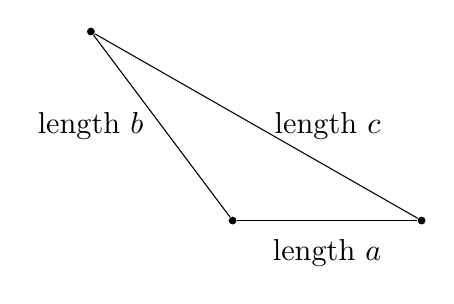
\begin{tikzpicture}[scale=1.2]
  \coordinate [circle, fill, inner sep=1pt] (a) at (1.5,0) ;
  \coordinate [circle, fill, inner sep=1pt] (b) at (0,2) ;
  \coordinate [circle, fill, inner sep=1pt] (c) at (3.5,0) ;
  \draw (a)--node[outer sep=3pt, left]{length $b$}(b) ;
  \draw (b)--node[outer sep=3pt, right]{length $c$}(c) ;
  \draw (c)--node[outer sep=3pt, below]{length $a$}(a) ;
\end{tikzpicture}

\section{Interior Angles of a Triangle}

We also talk a lot about the interior angles of a triangle:

\begin{tikzpicture}[scale=2]
  \coordinate [circle, fill, inner sep=2pt] (a) at (0,0) ;
  \coordinate [circle, fill, inner sep=2pt] (b) at (1, 2) ;
  \coordinate [circle, fill, inner sep=2pt] (c) at (3,0) ;
  \draw (a)--(b) node [outer sep=3pt, above]{$B$};
  \draw (b)--(c) node[outer sep=3pt, right]{$C$};
  \draw (c)--(a) node[outer sep=3pt, left]{$A$};
  \pic [draw, <->, "$a$", angle eccentricity=1.5] {angle = c--a--b};
  \pic [draw, <->, "$b$", angle eccentricity=1.5] {angle = a--b--c};
  \pic [draw, <->, "$c$", angle eccentricity=1.5] {angle = b--c--a};
\end{tikzpicture}

A triangle where one of the interior angles is a right angle is said to be a \emph{right triangle}:\index{right triangle}

\begin{tikzpicture}[scale=1.2]
  \coordinate [circle, fill, inner sep=2pt] (a) at (0,0) ;
  \coordinate [circle, fill, inner sep=2pt] (b) at (0,4) ;
  \coordinate [circle, fill, inner sep=2pt] (c) at (3,0) ;
  \draw (a)--(b) node [outer sep=3pt, above]{$B$};
  \draw (b)--(c) node[outer sep=3pt, right]{$C$};
  \draw (c)--(a) node[outer sep=3pt, left]{$A$};
  \pic [draw,angle eccentricity=1.5] {right angle = c--a--b};
\end{tikzpicture}

If a triangle has an obtuse interior angle, it is said to be an \emph{obtuse triangle}:\index{obtuse triange}

\begin{tikzpicture}[scale=1.2]
  \coordinate [circle, fill, inner sep=2pt] (a) at (1.5,0) ;
  \coordinate [circle, fill, inner sep=2pt] (b) at (0,2) ;
  \coordinate [circle, fill, inner sep=2pt] (c) at (3.5,0) ;
  \draw (a)--(b) node [outer sep=3pt, above]{$B$};
  \draw (b)--(c) node[outer sep=3pt, right]{$C$};
  \draw (c)--(a) node[outer sep=3pt, left]{$A$};
  \pic [draw, <->, "obtuse", angle eccentricity=1.7] {angle = c--a--b};
\end{tikzpicture}

If all three interior angles of a triangle are less than $90^\circ$, it is said to be an \emph{acute triangle}.\index{acute triangle}

The measures of the interior angles of a triangle always add up to
$180^\circ$. For example, if we know that a triangle has interior
angles of $37^\circ$ and $56^\circ$, we know that the third
interior angle is $87^\circ$.

\begin{Exercise}[title={Missing Angle}, label=missing_angle]
One interior angle of a triangle is $92^\circ$. The second angle is $42^\circ$. What is the measure of the third interior angle?
\end{Exercise}
\begin{Answer}[ref=missing_angle]
$180^\circ - (92^\circ + 42^\circ) = 46^\circ$
\end{Answer}

% Needs Diagram
How can you know that the sum of the interior angles is $180^\circ$?
Imagine that you started on the edge of a triangle and walked all the
way around to where you started. ( going
counter-clockwise.) You would turn three times to the left:

\begin{tikzpicture}[scale=1.7]
  \coordinate [circle, fill, inner sep=2pt] (a) at (1.5,0) ;  
   \node at (a) [outer sep=3pt, left]{$A$};
  \coordinate [circle, fill, inner sep=2pt] (b) at (0.5,2) ;
  \node at (b) [outer sep=3pt, above]{$B$} ;
  \coordinate [circle, fill, inner sep=2pt] (c) at (3.5,0) ;
    \node at (c)[outer sep=3pt, below]{$C$};
    
    \coordinate [circle, fill, inner sep=2pt](start) at (2.75,0);
    \node at (start)[outer sep=3pt, below]{Start};

   \coordinate (aa) at (1.75,-0.5) ;  
  \coordinate (bb) at (-0.25,2.5) ;
  \coordinate (cc) at (4.2,0) ;
  \draw [->](a)--(cc);
  \draw [->](b)--(aa);
  \draw [->](c)--(bb);
  \pic [draw, ->, "$T_C$", angle eccentricity=1.7] {angle = cc--c--b};
  \pic [draw, ->, "$T_B$", angle eccentricity=2] {angle = bb--b--a};
  \pic [draw, ->, "$T_A$", angle eccentricity=2] {angle = aa--a--c};
\end{tikzpicture}

After these three turns, you would be facing the same direction that
you started in. Thus $T_A + T_B + T_C = 360^\circ$. The
measures of the interior angles are $a$, $b$, and $c$. Notice that $a$ and
$T_A$ are supplementary. So we know that:
\begin{itemize}
\item $T_A = 180 - a$
\item $T_B = 180 - b$
\item $T_C = 180 - c$
\end{itemize}
So we can rewrite the equation above as
\begin{equation*}
  (180 - a) + (180 - b) + (180 - c) = 360^\circ
\end{equation*}
Which is equivalent to
\begin{equation*}
  a + b + c = 360^\circ
\end{equation*}

\begin{Exercise}[title={Interior Angles of a Quadrilateral}, label=interior_of_quad]
  Any four-sided polygon is a \emph{quadrilateral}. Using the same
  ``walk around the edge'' logic, what is the sum of the interior
  angles of any quadrilateral?
\end{Exercise}
\begin{Answer}[ref=interior_of_quad]
$360^\circ$
\end{Answer}


\graphicspath{{../../Chapters/pythagorean_theorem/en_US}}
\chapter{Pythagorean Theorem}

Watch's Khan Academy's Intro to the Pythagorean Theorem video at \url{https://youtu.be/AA6RfgP-AHU}.

If you have a right triangle, the edges that touch the right angle are
called \emph{the legs}.  The third edge, which is always the longest and opposite the right angle,
is known as \emph{the hypotenuse}. The Pythagorean Theorem gives us
the relationship between the length of the legs and the length of the
hypotenuse.

\begin{tikzpicture}[scale=1.2]
  \coordinate [circle, fill, inner sep=1pt] (a) at (0,0) ;
  \coordinate [circle, fill, inner sep=1pt] (b) at (0,4) ;
  \coordinate [circle, fill, inner sep=1pt] (c) at (3,0) ;
  \draw (a)--node [outer sep=3pt, left]{Length $a$}(b);
  \draw (b)--node[outer sep=3pt, right]{Length $c$}(c) ;
  \draw (c)--node[outer sep=3pt, below]{Length $b$}(a) ;
  \pic [draw, angle eccentricity=1.5] {right angle = c--a--b};
\end{tikzpicture}

The Pythagorean Theorem tells us that $a^2 + b^2 = c^2$.\index{Pythagorean theorem}

For example, if one leg has a length of 3 and the other has a length of 4, then
$a^2 + b^2 = 3^2 + 4^2 = 25$. Thus, $c^2$ must equal 25. This means you know
the hypotenuse must be of length 5. This works for any right triangle

In reality, it rarely works out to be such a tidy number. For
example, what is the length of the hypotenuse if the two legs are 3
and 6? $a^2 + b^2 = 3^2 + 6^2 = 45$.  The length of the hypotenuse is
the square root of that: $\sqrt{45} = \sqrt{9 \times 5} = 3 \sqrt{5}$,
which is approximately 6.708203932499369.

Common side lengths for these triangles are referred to as \emph{Pythagorean triples}\index{Pythagorean triples}, meaning they evaluate to a whole number. Some common examples are $(3, 4, 5)$, $(5, 12, 13)$, and $(8, 15, 17)$. Multiples of right triangles are also triangles ie. $(3, 4, 5) \implies (6, 8, 10)$, which we will touch on next chapter.

There are also angle-based right triangles, consisting of ratios of the angles of the triangles. The most common ones are $45^\circ$-$45^\circ$-$90^\circ$ and the $30^\circ$-$60^\circ$-$90^\circ$. We will discuss these further in depth, but know for now that they are vital in trigonometry, and consist of Pythagorean triples as side lengths. 

\begin{Exercise}[title={Find the Missing Length}, label=missingsides]
  What is the missing measure?
  % this formatting seems to be messed up
  \begin{multicols}{2}
Leg 1 = 6, Leg 2 = 8, Hypotenuse = ? \\(It should be a whole number.)

Leg 1 = 5, Leg 2 = ?, Hypotenuse = 13 \\(It should be a whole number.)
  
Leg 1 = ?, Leg 2 = 15, Hypotenuse = 17 \\(It should be a whole number.)

Leg 1 = 3, Leg 2 = 3, Hypotenuse = ? \\(It is an irrational number. Give the exact answer and then use a calculator to get an approximation.)
\end{multicols}
\end{Exercise}
\begin{Answer}[ref=missingsides]
  10 because $6^2 + 8^2 = 10^2$

  12 because $5^2 + 12^2 = 13^2$

  8 because $8^2 + 15^2 = 17^2$

  $3\sqrt{2} \approx 4.24$ because $3^2 + 3^2 = \left(3 \sqrt{2}\right)^2$
\end{Answer}


\section{Distance between Points}

What is the distance between these two points?\index{distance using Pythagorean theorem}

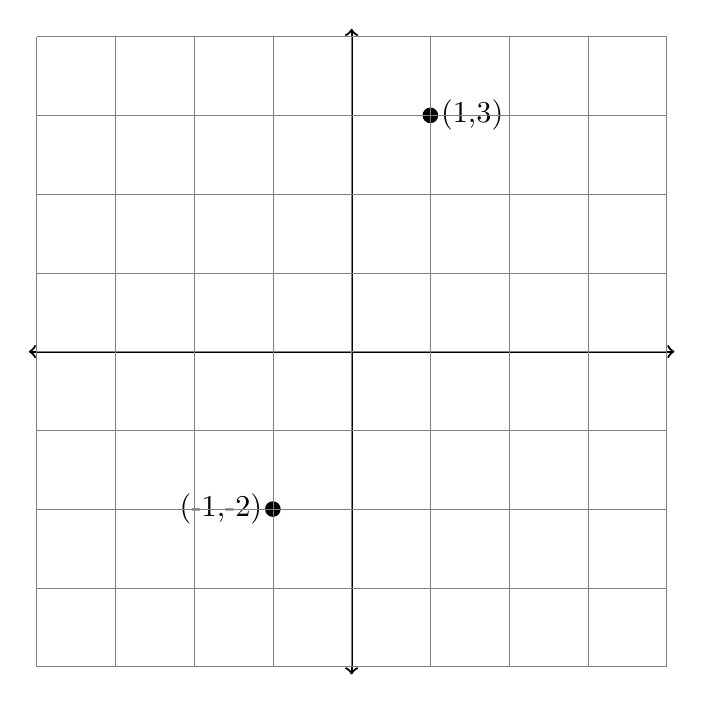
\begin{tikzpicture}
  % axis
  \draw[thick, <->] (0, -4.1) -- (0, 4.1);
  \draw[thick, <->] (-4.1, 0) -- (4.1, 0);
  \coordinate [circle, fill, inner sep=2pt] (a) at (-1,-2) ;
  \coordinate [circle, fill, inner sep=2pt] (b) at (1,3) ;
  \node [left] at (a) {(-1,-2)};
  \node [right] at (b) {(1,3)};
  % grid
  \draw[help lines, step = 1cm] (-4, -4) grid (4, 4);
  
\end{tikzpicture}

We can draw a right triangle and use the Pythagorean Theorem:

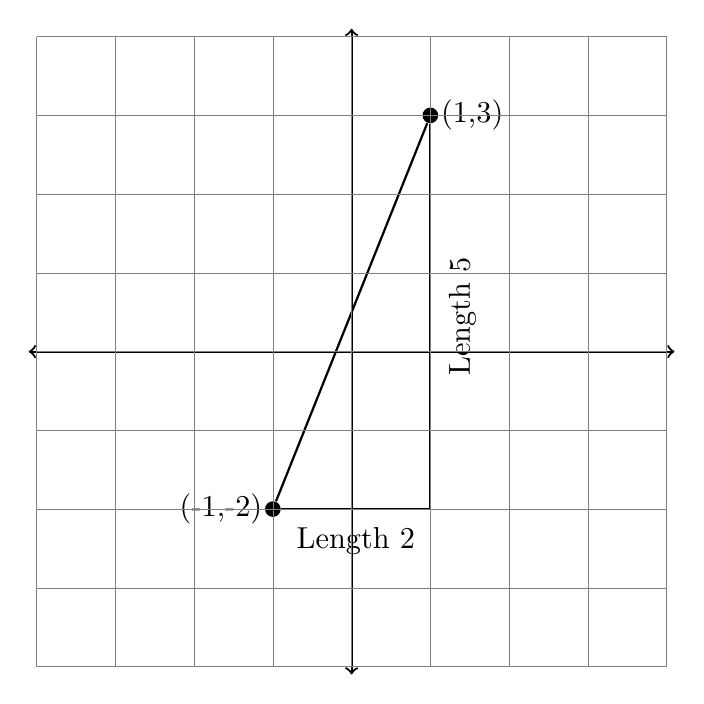
\begin{tikzpicture}
  % axis
  \draw[thick, <->] (0, -4.1) -- (0, 4.1);
  \draw[thick, <->] (-4.1, 0) -- (4.1, 0);
  \coordinate [circle, fill, inner sep=2pt] (a) at (-1,-2) ;
  \coordinate [circle, fill, inner sep=2pt] (b) at (1,3) ;
    \node [left] at (a) {(-1,-2)};
  \node [right] at (b) {(1,3)};
  \coordinate (c) at (1, -2);

  \draw [thick] (a) -- (b);
  \draw [thick] (a) -- node[outer sep = 3pt, below]{Length 2}(c);
  \draw [thick] (c) -- node[rotate=90, outer sep = 3pt, below]{Length 5}(b);
  \draw[help lines, step = 1cm] (-4, -4) grid (4, 4);
 
\end{tikzpicture}


The distance between the two points is $\sqrt{2^2 + 5^2} = \sqrt{29}
\approx 5.385165$. In other words, you square the change in $x$ and add it to
the square of the change in $y$. The distance is the square root of
that sum.

\section{Distance in 3 Dimensions}

What if the point is in three-dimensional space?  For example, you move 2
meters East, 8 meters North, and 4 meters up in the air. How far are
you from where you started?  You just square each, sum them, and take the square root:
$\sqrt{2^2 + 8^2 + 4^2} = \sqrt{84} = 2\sqrt{21} \approx 9.165$ meters.\index{distance!in 3 dimensions}

\begin{tikzpicture}
  \draw [thick, ->] (0,0,0) -- (9,0,0) node[outer sep = 1pt, right]{North} ; 
  \draw [thick, ->]  (0,0,0) -- (0,3,0) node[outer sep = 1pt, above]{Up} ; 
  \draw [thick, ->] (0,0,0) -- (0,0,4) node[outer sep = 1pt, below]{East} ; 

    \draw [dashed]  (8,0,0) -- node[outer sep = 1pt, right]{2}  (8,0,2); 

  \draw [dashed]  (0,0,2) -- node[outer sep = 1pt, below]{8} (8,0,2); 
  \draw [dashed]  (8,0,2) -- node[outer sep = 1pt, right]{4} (8,4,2); 
  \draw [thick]  (0,0,0) --  (8,4,2) node[circle, fill, inner sep=2pt]{}; 
  \node [left] at (5, 2.7, 1){$\sqrt{2^2 + 8^2 + 4^2} \approx 9.165$};

\end{tikzpicture}

This leads us to a formal definition of the distance formula:
\[
d = \sqrt{(x_2 - x_1)^2 + (y_2 - y_1)^2}
\]
Or in 3D space:
\[
d = \sqrt{(x_2 - x_1)^2 + (y_2 - y_1)^2 + (z_2 - z_1)^2}
\]

\graphicspath{{../../Chapters/congruence/en_US}}
\chapter{Congruence}
% Add: simple triangles
%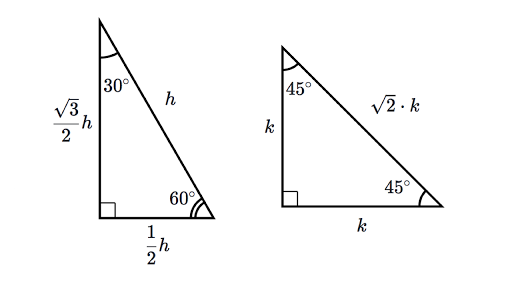
\includegraphics[width=0.8\textwidth]{KA_Special_Triangles.png}
Look at this picture of two geometric figures.

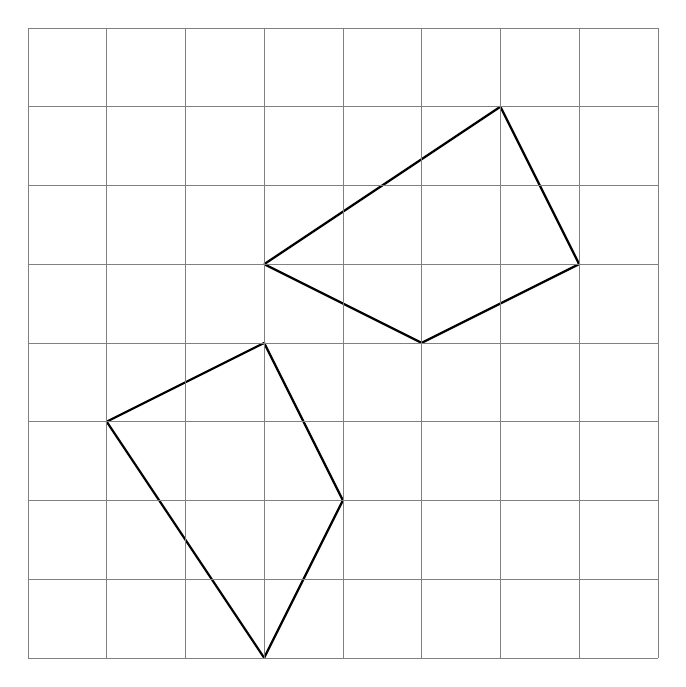
\begin{tikzpicture}
 
  	\draw [thick] (-1,-4) --  (0, -2);
	\draw [thick] (0,-2) --  (-1, 0) ;
	\draw [thick] (-1,0) --  (-3, -1); 
	\draw [thick] (-3,-1) --  (-1, -4);
	
	\draw [thick] (-1,1) --  (1, 0);
	\draw [thick] (1,0) --  (3, 1) ;
	\draw [thick] (3,1) --  (2, 3); 
	\draw [thick] (2,3) --  (-1, 1);

  \draw[help lines, step = 1cm] (-4, -4) grid (4, 4);
 
\end{tikzpicture}

They are the same shape, right? If you cut one out with scissors, it
would lay perfectly on top of the other. In geometry, we say they are
\emph{congruent}.

What is the official definition of ``congruent''? 
Two geometric figures are congruent if you can transform one into the other using
only rigid transformations. 

You might be wondering now, what are rigid transformations?
A transformation is \emph{Rigid} if it doesn't change the distances
between the points or the measure of the angles between the lines, they
form. These are all rigid transformations:
\begin{itemize}
\item Translations
\item Rotations
\item Reflections 
\end{itemize}

Once again imagine cutting out one figure with scissors and trying to match it with the second figure, your actions are rigid transformations:
\begin{itemize}
\item Translations - sliding the cutout left and right and up and down
\item Rotations	- rotating the cutout clockwise and counterclockwise
\item Reflection - flipping the piece of paper over
\end{itemize}

A transformation is rigid if it is some combination of translations, rotations, and reflections.

\section{Triangle Congruency}

If the sides of two triangles have the same length, the triangles must be congruent:

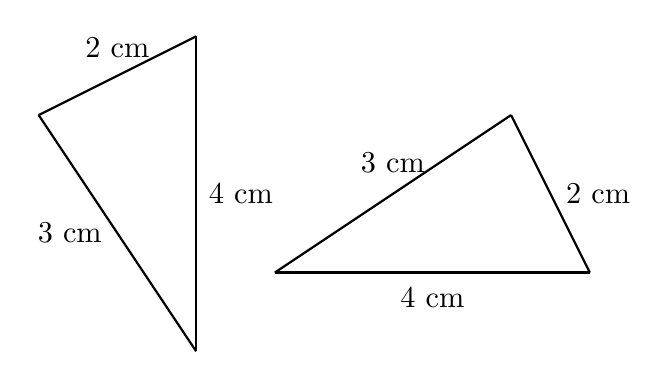
\begin{tikzpicture} 
  	\draw [thick] (-2,0) -- node[outer sep = 1pt, right]{4 cm}  (-2, 4) ;
	\draw [thick] (-2,4) --  node[outer sep = 3pt, above]{2 cm} (-4, 3); 
	\draw [thick] (-4,3) --  node[outer sep = 2pt, left]{3 cm} (-2, 0);
	
	\draw [thick] (-1,1) --  node[outer sep = 2pt, below]{4 cm}  (3, 1) ;
	\draw [thick] (3,1) --  node[outer sep = 2pt, right]{2 cm} (2, 3); 
	\draw [thick] (2,3) --  node[outer sep = 4pt, above]{3 cm} (-1, 1);
\end{tikzpicture}

To be precise, the Side-Side-Side Congruency Test says that two triangles are
congruent if three sides in one triangle are the same length as the
corresponding sides in the other. We usually refer to this as the SSS test.
% Explain with a^2 + b^2 = c^2

Note that two triangles with all three angles equal are not necessarily congruent.
For example, here are two triangles with the same interior angles, but they are
different sizes:

\begin{tikzpicture}
  \coordinate [circle, fill, inner sep=1pt] (a1) at (0,0) ;
  \coordinate [circle, fill, inner sep=1pt] (b1) at (4,0) ;
  \coordinate [circle, fill, inner sep=1pt] (c1) at (3,2) ;
  
   \coordinate [circle, fill, inner sep=1pt] (a2) at (5,0) ;
  \coordinate [circle, fill, inner sep=1pt] (b2) at (11,0) ;
  \coordinate [circle, fill, inner sep=1pt] (c2) at (9.5,3) ;
        \draw (a1) --   (b1);
        \draw (b1) -- (c1);
        \draw (c1)--  (a1);
        \pic [draw, "$63^\circ$", angle eccentricity=1.5] {angle = c1--b1--a1};
        \pic [draw, "$34^\circ$", angle eccentricity=2.0] {angle = b1--a1--c1};
        \pic [draw, "$83^\circ$", angle eccentricity=1.5] {angle = a1--c1--b1};

       \draw (a2) --  (b2);
        \draw (b2) -- (c2);
        \draw (c2)--  (a2);
        \pic [draw, "$63^\circ$", angle eccentricity=1.5] {angle = c2--b2--a2};
        \pic [draw, "$34^\circ$", angle eccentricity=2.0] {angle = b2--a2--c2};
        \pic [draw, "$83^\circ$", angle eccentricity=1.5] {angle = a2--c2--b2};

\end{tikzpicture}

These triangles are not congruent, but they are \emph{similar}. Meaning
 they have the same shape, but are not necessarily the same
size.

Therefore, if you know two angles of a triangle, you can calculate the third. So it makes sense
to say ``If two triangles have two angles that are equal, they are
similar triangles.''  And if two similar triangles have one side that
is equal in length, they must be the same size -- so they are
congruent. Thus, the Side-Angle-Angle Congruency Test says that
two triangles are congruent if two angles and one side match.

What if you know that two triangles have two sides that are the same
length and that the angle between them is also equal?

\begin{tikzpicture}
  \coordinate [circle, fill, inner sep=1pt] (a1) at (0,0) ;
  \coordinate [circle, fill, inner sep=1pt] (b1) at (4,0) ;
  \coordinate [circle, fill, inner sep=1pt] (c1) at (3,2) ;
  
  \coordinate [circle, fill, inner sep=1pt] (a2) at (5,0) ;
  \coordinate [circle, fill, inner sep=1pt] (b2) at (9,0) ;
  \coordinate [circle, fill, inner sep=1pt] (c2) at (8,2) ;
  
  \draw (a1) --  node[outer sep = 0.5pt, below]{4}  (b1);
  \draw [dashed] (b1) -- (c1);
  \draw (c1)--  node[outer sep = 5pt, above]{3.5} (a1);
  \pic [draw, "$34^\circ$", angle eccentricity=2.0] {angle = b1--a1--c1};

  \draw (a2) --  node[outer sep = 0.5pt, below]{4}  (b2);
  \draw [dashed] (b2) -- (c2);
  \draw (c2)--  node[outer sep = 5pt, above]{3.5} (a2);
  \pic [draw, "$34^\circ$", angle eccentricity=2.0] {angle = b2--a2--c2};
\end{tikzpicture}

Yes, they must be congruent. This is the Side-Angle-Size Congruency Test.

What if the angle isn't the one between the two known sides? If it is
a right angle, you can be certain the two triangles are congruent.
(How do I know? Because the Pythagorean Theorem tells us that we can
calculate the length of the third side. There is only one possibility,
thus all three sides must be the same length.)

\begin{tikzpicture}
  \coordinate [circle, fill, inner sep=1pt] (a1) at (0,0) ;
  \coordinate [circle, fill, inner sep=1pt] (b1) at (4,0) ;
  \coordinate [circle, fill, inner sep=1pt] (c1) at (4,2) ;
  
   \coordinate [circle, fill, inner sep=1pt] (a2) at (5,0) ;
  \coordinate [circle, fill, inner sep=1pt] (b2) at (9,0) ;
  \coordinate [circle, fill, inner sep=1pt] (c2) at (9,2) ;
        \draw (a1) --  node[outer sep = 0.5pt, below]{3.5}  (b1);
        \draw [dashed] (b1) -- (c1);
        \draw (c1)--  node[outer sep = 5pt, above]{4} (a1);
        \pic [draw] {right angle = a1--b1--c1};

        \draw (a2) --  node[outer sep = 0.5pt, below]{3.5}  (b2);
        \draw [dashed] (b2) -- (c2);
        \draw (c2)--  node[outer sep = 5pt, above]{4} (a2);
        \pic [draw] {right angle = a2--b2--c2};
\end{tikzpicture}

In this case, the third side of each triangle must be $\sqrt{4^2 - 3.5^2} \approx 1.9$.

What if the know angle is less than $90^\circ$? \emph{The triangles
  are not necessarily congruent.} For example, let's say that there are
two triangles with sides of length 5 and 7 and that the corresponding
angle (at the end of the side of length 7) on each is $45^\circ$. Two
different triangles satisfy this:

\begin{tikzpicture}
  \coordinate [circle, fill, inner sep=1pt] (a1) at (0,0) ;
  \coordinate [circle, fill, inner sep=1pt] (b1) at (7,0) ;
  \coordinate [circle, fill, inner sep=1pt] (c1) at (4,3) ;
  \coordinate [circle, fill, inner sep=1pt] (a2) at (8,0) ;
  \coordinate [circle, fill, inner sep=1pt] (b2) at (15,0) ;
  \coordinate [circle, fill, inner sep=1pt] (c2) at (11,4) ;
  \draw (a1) --  node[outer sep = 0.5pt, below]{7}  (b1);
  \draw [dashed] (b1) -- (c1);
  \draw (c1)--  node[outer sep = 5pt, above]{5}(a1);
  \pic [draw, "$45^\circ$", angle eccentricity=1.5] {angle = c1--b1--a1};
  \draw (a2) --  node[outer sep = 0.5pt, below]{7}  (b2);
  \draw [dashed] (b2) -- (c2);
  \draw (c2)--  node[outer sep = 5pt, above]{5} (a2);
  \pic [draw, "$45^\circ$", angle eccentricity=1.5] {angle = c2--b2--a2};
\end{tikzpicture}

Let's see this another way by laying one triangle on top of the other:

\begin{tikzpicture}
  \coordinate [circle, fill, inner sep=1pt] (a1) at (0,0) ;
  \coordinate [circle, fill, inner sep=1pt] (b1) at (7,0) ;
  \coordinate [circle, fill, inner sep=1pt] (c1) at (4,3) ;
  \coordinate [circle, fill, inner sep=1pt] (c2) at (3,4) ;
  \coordinate (d) at (2,5);
  \coordinate (e) at (3.5,3.5);

  \draw (a1) --  node[outer sep = 0.5pt, below]{7}  (b1);
  \draw [dashed,->] (b1) -- (d);
  \draw [dashed] (a1) -- (e);
  \draw (c1)--  node[outer sep = 5pt, below]{5}(a1);
  \draw (c2)--  node[outer sep = 5pt, above]{5}(a1);
  \pic [draw, "$45^\circ$", angle eccentricity=1.5] {angle = c1--b1--a1};
   \pic [draw, angle radius=8] {right angle = b1--e--a1};
\end{tikzpicture}


So there is \emph{not} a general Side-Side-Angle Congruency Test.

Here, then, is the list of common congruency tests:
\begin{itemize}
\item Side-Side-Side: All three sides have the same measure
\item Side-Angle-Angle: Two angles and one side have the same measure
\item Side-Angle-Side: Two sides and the angle between them have the same measure
\item Side-Side-Right: They are right triangles and have two sides have the same measure
\end{itemize}

\begin{Exercise}[title={Congruent Triangles}, label=con_triangles]
  Ted is terrible at drawing triangles: he always draws them exactly
  the same. Fortunately, he has marked these diagrams with the sides
  and angles that he measured. For each pair of triangles, write if
  you know them to be congruent and which congruency test proves
  it. For example:

\begin{tikzpicture}[scale=0.7]
  \coordinate [circle, fill, inner sep=1pt] (a1) at (0,1) ;
  \coordinate [circle, fill, inner sep=1pt] (b1) at (5,0) ;
  \coordinate [circle, fill, inner sep=1pt] (c1) at (4,2) ;
  
  \coordinate [circle, fill, inner sep=1pt] (a2) at (6,1) ;
  \coordinate [circle, fill, inner sep=1pt] (b2) at (11,0) ;
  \coordinate [circle, fill, inner sep=1pt] (c2) at (10,2) ;
  \draw (a1) --  node[outer sep = 0.5pt, below]{3.5}  (b1);
  \draw (b1) -- node[outer sep = 2pt, right]{4} (c1);
  \draw (c1)--  node[outer sep = 2pt, above]{} (a1);
  \pic [draw,  "$120^\circ$", angle eccentricity=2.0] {angle = c1--b1--a1};

  \draw (a2) --  node[outer sep = 0.5pt, below]{3.5}  (b2);
  \draw  (b2) -- node[outer sep = 2pt, right]{4} (c2);
  \draw (c2) -- node[outer sep = 2pt, above]{} (a2);
  \pic [draw,  "$120^\circ$",, angle eccentricity=2.0] {angle = c2--b2--a2};
\end{tikzpicture}

  (These drawings are clearly not accurate, but you are told the measurements are.) The answer is ``Congruent by the Side-Angle-Side test.''

  \begin{multicols}{2}

\begin{tikzpicture}[scale=0.6]
  \coordinate [circle, fill, inner sep=1pt] (a1) at (0,1) ;
  \coordinate [circle, fill, inner sep=1pt] (b1) at (5,0) ;
  \coordinate [circle, fill, inner sep=1pt] (c1) at (4,2) ;
  
  \coordinate [circle, fill, inner sep=1pt] (a2) at (6,1) ;
  \coordinate [circle, fill, inner sep=1pt] (b2) at (11,0) ;
  \coordinate [circle, fill, inner sep=1pt] (c2) at (10,2) ;
  \draw (a1) --  node[outer sep = 0.5pt, below]{3.5}  (b1);
  \draw (b1) -- node[outer sep = 2pt, right]{} (c1);
  \draw (c1)--  node[outer sep = 2pt, above]{6} (a1);
  \pic [draw,  "$90^\circ$", angle eccentricity=2.0] {angle = c1--b1--a1};

  \draw (a2) --  node[outer sep = 0.5pt, below]{3.5}  (b2);
  \draw  (b2) -- node[outer sep = 2pt, right]{} (c2);
  \draw (c2) -- node[outer sep = 2pt, above]{6} (a2);
  \pic [draw,  "$90^\circ$",, angle eccentricity=2.0] {angle = c2--b2--a2};
\end{tikzpicture}

\hspace{3cm}

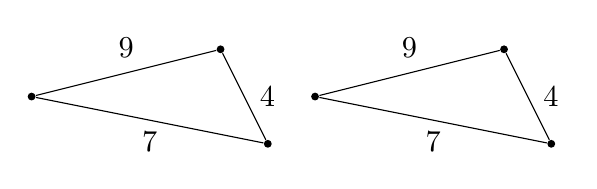
\begin{tikzpicture}[scale=0.6]
  \coordinate [circle, fill, inner sep=1pt] (a1) at (0,1) ;
  \coordinate [circle, fill, inner sep=1pt] (b1) at (5,0) ;
  \coordinate [circle, fill, inner sep=1pt] (c1) at (4,2) ;
  
  \coordinate [circle, fill, inner sep=1pt] (a2) at (6,1) ;
  \coordinate [circle, fill, inner sep=1pt] (b2) at (11,0) ;
  \coordinate [circle, fill, inner sep=1pt] (c2) at (10,2) ;
  \draw (a1) --  node[outer sep = 0.5pt, below]{7}  (b1);
  \draw (b1) -- node[outer sep = 2pt, right]{4} (c1);
  \draw (c1)--  node[outer sep = 2pt, above]{9} (a1);

  \draw (a2) --  node[outer sep = 0.5pt, below]{7}  (b2);
  \draw  (b2) -- node[outer sep = 2pt, right]{4} (c2);
  \draw (c2) -- node[outer sep = 2pt, above]{9} (a2);
\end{tikzpicture}


\begin{tikzpicture}[scale=0.6]
  \coordinate [circle, fill, inner sep=1pt] (a1) at (0,1) ;
  \coordinate [circle, fill, inner sep=1pt] (b1) at (5,0) ;
  \coordinate [circle, fill, inner sep=1pt] (c1) at (4,2) ;
  
  \coordinate [circle, fill, inner sep=1pt] (a2) at (6,1) ;
  \coordinate [circle, fill, inner sep=1pt] (b2) at (11,0) ;
  \coordinate [circle, fill, inner sep=1pt] (c2) at (10,2) ;
  \draw (a1) --  node[outer sep = 0.5pt, below]{7}  (b1);
  \draw (b1) -- node[outer sep = 2pt, right]{} (c1);
  \draw (c1)--  node[outer sep = 2pt, above]{} (a1);
  \pic [draw,  "$35^\circ$",, angle eccentricity=2.0] {angle = c1--b1--a1};
  \pic [draw,  "$62^\circ$",, angle eccentricity=2.0] {angle = b1--a1--c1};

  \draw (a2) --  node[outer sep = 0.5pt, below]{7}  (b2);
  \draw  (b2) -- node[outer sep = 2pt, right]{} (c2);
  \draw (c2) -- node[outer sep = 2pt, above]{} (a2);
  \pic [draw,  "$35^\circ$",, angle eccentricity=2.0] {angle = c2--b2--a2};
  \pic [draw,  "$62^\circ$",, angle eccentricity=2.0] {angle = b2--a2--c2};

\end{tikzpicture}

\hspace{3cm}


\begin{tikzpicture}[scale=0.6]
  \coordinate [circle, fill, inner sep=1pt] (a1) at (0,1) ;
  \coordinate [circle, fill, inner sep=1pt] (b1) at (5,0) ;
  \coordinate [circle, fill, inner sep=1pt] (c1) at (4,2) ;
  
  \coordinate [circle, fill, inner sep=1pt] (a2) at (6,1) ;
  \coordinate [circle, fill, inner sep=1pt] (b2) at (11,0) ;
  \coordinate [circle, fill, inner sep=1pt] (c2) at (10,2) ;
  \draw (a1) --  node[outer sep = 0.5pt, below]{8}  (b1);
  \draw (b1) -- node[outer sep = 2pt, right]{6} (c1);
  \draw (c1)--  node[outer sep = 2pt, above]{} (a1);
  \pic [draw,  "$28^\circ$",, angle eccentricity=2.0] {angle = b1--a1--c1};

  \draw (a2) --  node[outer sep = 0.5pt, below]{8}  (b2);
  \draw  (b2) -- node[outer sep = 2pt, right]{6} (c2);
  \draw (c2) -- node[outer sep = 2pt, above]{} (a2);
  \pic [draw,  "$28^\circ$",, angle eccentricity=2.0] {angle = b2--a2--c2};

\end{tikzpicture}


\end{multicols}
\end{Exercise}

\begin{Answer}[ref=con_triangles]
\begin{multicols}{2}
Congruent by the Side-Side-Right Congruency Test.

Congruent by the Side-Side-Side Congruency Test.

Congruent by the Side-Angle-Angle Congruency Test.

We don't know if they are congruent. The measured angle is not between the measured sides.

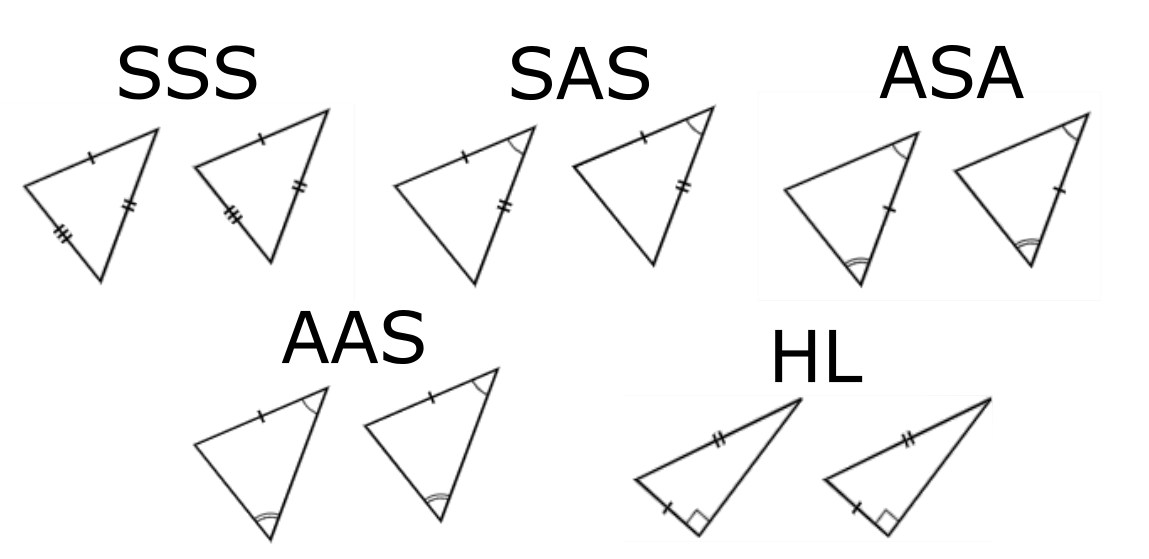
\includegraphics[width=0.8\textwidth]{Triangle_Congruence.png}
\end{multicols}

\end{Answer}




\graphicspath{{../../Chapters/vectors/en_US}}
\chapter{Vectors}

We have talked a some about forces, but in the calculations that we
have done, we have only talked about the magnitude of a force. It is
equally important to talk about its direction. To do the math on
things with a magnitude and a direction (like forces), we need vectors.\index{vectors}

For example, if you jump out of a plane (hopefully with a parachute), 
several forces with different magnitudes and directions will be acting upon 
you. Gravity will push you straight down. That force will be proportional to your weight.
If there were a wind from the west, it would push you toward the east. That force
will be proportional to the square of the speed of the wind and approximately proportional to 
your size. Once you are falling, there will be resistance from the air 
that you are pushing through -- that force will point in the opposite direction
from the direction you are moving and will be proportional to the square of your
speed.

To figure out the net force (which will tell us how we will accelerate), we will 
need to add these forces together. So we need to learn to do math with vectors.

\section{Adding Vectors}

A vector is typically represented as a list of numbers, with each
number representing a particular dimension. For example, if I am
creating a 3-dimensional vector representing a force, it will have
three numbers representing the amount of force in each of the three
axes. For example, if a force of one newton is in the direction of the
$x$-axis, I might represent the vector as $v = [1, 0, 0]$. 
Another vector might be $u = [0.5, 0.9, 0.7]$ \index{vectors!adding}

\tdplotsetmaincoords{80}{130} 
\begin{tikzpicture} [scale=4, tdplot_main_coords, axis/.style={->,sdkblue}, 
vector/.style={-stealth,black,very thick}, 
vector guide/.style={dashed,sdkblue}]

%standard tikz coordinate definition using x, y, z coords
\coordinate (O) at (0,0,0);

%draw axes
\draw[axis] (0,0,0) -- (1.5,0,0) node[anchor=north east]{$x$};
\draw[axis] (0,0,0) -- (0,0.9,0) node[anchor=north west]{$y$};
\draw[axis] (0,0,0) -- (0,0,0.9) node[anchor=south]{$z$};

%draw a vector from O to P
\draw[vector] (O) -- (1,0,0);
\draw[vector] (O) -- (0.5,0.9,0.7);
\draw (0.2,0.0,0.05) node[left] {v};
\draw (0.2,0.35,0.3) node[right] {u};

\draw[vector guide] (0.5,0,0) -- (0.5,0.9,0);
\draw[vector guide] (0.0,0.9,0) -- (0.5,0.9,0);
\draw[vector guide] (0.5,0.9,0) -- (0.5,0.9,0.7);
\end{tikzpicture}

Thinking visually, when we add to vectors, we put the starting point 
second vector at the ending point of the first vector.


\tdplotsetmaincoords{80}{130} 
\begin{tikzpicture} [scale=4, tdplot_main_coords, axis/.style={->,sdkblue}, 
light vector/.style={-stealth,dashed,very thick, black}, 
vector/.style={-stealth,black,very thick}, 
vector guide/.style={dashed,sdkblue}]

%standard tikz coordinate definition using x, y, z coords
\coordinate (O) at (0,0,0);

%draw axes
\draw[axis] (0,0,0) -- (1.5,0,0) node[anchor=north east]{$x$};
\draw[axis] (0,0,0) -- (0,0.9,0) node[anchor=north west]{$y$};
\draw[axis] (0,0,0) -- (0,0,0.9) node[anchor=south]{$z$};

%draw a vector from O to P
\draw[light vector] (0,0,0) -- (0.5,0.9,0.7);
\draw[light vector] (0.5, 0.9, 0.7) -- (1.5, 0.9, 0.7);
\draw[vector] (0,0,0) -- (1.5,0.9,0.7) node[left] {u + v};
\draw (0.7,0.9,0.75) node[left] {v};
\draw (0.2,0.35,0.3) node[right] {u};

\draw[vector guide] (0.5,0,0) -- (0.5,0.9,0);
\draw[vector guide] (0.0,0.9,0) -- (0.5,0.9,0);
\draw[vector guide] (0.5,0.9,0) -- (0.5,0.9,0.7);
\draw[vector guide] (0.5,0.9,0) -- (1.5,0.9,0.0);
\draw[vector guide] (1.5,0.9,0.0) -- (1.5,0.9,0.7);
\draw[vector guide] (1.5,0.0,0.0) -- (1.5,0.9,0.0);

\end{tikzpicture}

If you know the vectors, you will just add them element-wise:

$$ u + v = [0.5, 0.9, 0.7] + [1.0, 0.0, 0.0] = [1.5, 0.9. 0.7] $$

These vectors have 3 components, so we say they are \newterm{3-dimensional}. 
Vectors can have any number of components. For example, the vector
 $[-12.2, 3, \pi, 10000]$ is 4-dimensional.

 You can only add two vectors if they have the same dimension.

 $$ [12, -4] + [-1, 5] = [11,1] $$

 Addition is commutative: If you have two vectors $a$ and $b$, then
 $a + b$ is the same as $b + a$.

 Addition is also associative: If you have three vectors $a$, $b$, and $c$,
 it doesn't matter which order you add them in. 
 That is, $a + (b + c) = (a + b) + c$.

 A 1-dimensional vector is just a number.  We say it is a 
 \newterm{scalar}, not a vector.

 \begin{Exercise}[title={Adding vectors}, label=adding_vectors]
Add the following vectors:
\begin{itemize}
    \item $[1, 2, 3] + [4, 5, 6]$
    \item $[-1, -2, -3, -4] + [4, 5, 6, 7]$
    \item $[\pi, 0, 0] + [0, \pi, 0] + [0, 0, \pi]$
\end{itemize}
\end{Exercise}
\begin{Answer}[ref=adding_vectors]
    \begin{itemize}
        \item $[1, 2, 3] + [4, 5, 6] = [5, 7, 9]$
        \item $[-1, -2, -3, -4] + [4, 5, 6, 7] = [3, 3, 3, 3]$
        \item $[\pi, 0, 0] + [0, \pi, 0] + [0, 0, \pi] = [\pi, \pi, \pi]$ 
    \end{itemize}
\end{Answer}

    \begin{Exercise}[title={Adding Forces}, label=adding_forces]
        You are adrift in space. You are near two different stars. 
        The gravity of one star is pulling you towards it with a 
        force of $[4.2, 5.6, 9.0]$ newtons.
        The gravity of the other star is pulling you towards it with
        a force of $[-100.2, 30.2, -9.0]$ newtons. What is the net force?
        \end{Exercise}
        \begin{Answer}[ref=adding_forces]
            To get the net force, you add the two forces:

            $$F = [4.2, 5.6, 9.0] + [-100.2, 30.2, -9.0] = [-96, 35.8, 0.0] \text{ newtons}$$
   
\end{Answer}

\section{Multiplying a vector with a scalar}

It is not uncommon to multiply a vector by a scalar.  For example, a rocket engine
might have a force vector $v$.  If you fire 9 engines in the exact same direction,
the resulting force vector would be $9v$.\index{vectors!multipying by a scalar}

Visually, when we multiply a vector $u$ by a scalar $a$, we get a new vector that
goes in the same direction as $u$ but has a magnitude $a$ times as long as $u$.

\tdplotsetmaincoords{80}{130} 
\begin{tikzpicture} [scale=3, tdplot_main_coords, axis/.style={->,sdkblue}, 
vector/.style={-stealth,black,very thick}, 
vector guide/.style={dashed,sdkblue}]

%standard tikz coordinate definition using x, y, z coords
\coordinate (O) at (0,0,0);

%draw axes
\draw[axis] (0,0,0) -- (1.6,0,0) node[anchor=north east]{$x$};
\draw[axis] (0,0,0) -- (0,2.8,0) node[anchor=north west]{$y$};
\draw[axis] (0,0,0) -- (0,0,1.9) node[anchor=south]{$z$};

%draw a vector from O to P
\draw[vector] (O) -- (0.5,0.9,0.7);
\draw (0.2,0.35,0.3) node[right] {$u$};

\draw[vector] (O) -- (1.5,2.7,2.1) node[right] {$3u$};


\draw[vector guide] (0.5,0,0) -- (0.5,0.9,0);
\draw[vector guide] (0.0,0.9,0) -- (0.5,0.9,0);
\draw[vector guide] (0.5,0.9,0) -- (0.5,0.9,0.7);

\draw[vector guide] (1.5,0,0) -- (1.5,2.7,0);
\draw[vector guide] (0.0,2.7,0) -- (1.5,2.7,0);
\draw[vector guide] (1.5,2.7,0) -- (1.5,2.7,2.1);
\end{tikzpicture}

When you multiply a vector by a scalar, you just multiply each of the components by the scalar:

$$ 3 \times [0.5, 0.9, 0.7] = [1.5, 2.7, 3.6] $$

\begin{Exercise}[title={Multiplying a vector and a scalar}, label=mult_scalar]
    Simplify the following expressions:
    \begin{itemize}
        \item $2 \times [1, 2, 3]$
        \item $[-1, -2, -3, -4] \times -2$
        \item $\pi[\pi, 2\pi, 3\pi]$
    \end{itemize}
    \end{Exercise}
    \begin{Answer}[ref=mult_scalar]
        \begin{itemize}
            \item $2 \times [1, 2, 3] = [2, 4, 6]$
            \item $[-1, -2, -3, -4] \times -3 = [3, 6, 9, 12]$
            \item $\pi[\pi, 2\pi, 3\pi]  = \pi^2, 2\pi^2, 3\pi^2]$ 
        \end{itemize}
    \end{Answer}

Note that when you multiply a vector times a negative number, the new vector points 
in the opposite direction.

\tdplotsetmaincoords{80}{130} 
\begin{tikzpicture} [scale=5, tdplot_main_coords, axis/.style={->,sdkblue}, 
vector/.style={-stealth,black,very thick}, 
vector guide/.style={dashed,sdkblue}]

%standard tikz coordinate definition using x, y, z coords
\coordinate (O) at (0,0,0);

%draw axes
\draw[axis] (0,0,0) -- (0.55,0,0) node[anchor=north east]{$x$};
\draw[axis] (0,0,0) -- (0,0.95,0) node[anchor=north west]{$y$};
\draw[axis] (0,0,0) -- (0,0,0.6) node[anchor=south]{$z$};

%draw a vector from O to P
\draw[vector] (O) -- (0.5,0.9,0.7);
\draw (0.2,0.36,0.3) node[right] {$u$};

\draw[vector] (O) -- (-0.25,-0.45,-0.35) node[right] {$(-0.5)u$};

\draw[vector guide] (0.5,0,0) -- (0.5,0.9,0);
\draw[vector guide] (0.0,0.9,0) -- (0.5,0.9,0);
\draw[vector guide] (0.5,0.9,0) -- (0.5,0.9,0.7);

\draw[vector guide] (-0.25,0,0) -- (-0.25,-0.45,0);
\draw[vector guide] (0,0,0) -- (-0.25,0,0);
\draw[vector guide] (0.0,-0.45,0) -- (-0.25,-0.45,0);
\draw[vector guide] (0,0,0) -- (0,-0.45,0);

\draw[vector guide] (-.25,-0.45,0) -- (-0.25,-0.45,-0.35);
\end{tikzpicture}

\section{Vector Subtraction}

As you might guess, when you subtract one vector from another, 
you just do element-wise subtraction:\index{vectors!subtraction}

$$[4,2,0] - [3,-2, 9] = [1, 4, -9]$$

So, $u - v = u + (-1v)$.

So visually, you reverse the one that is being subtracted:


\tdplotsetmaincoords{80}{130} 
\begin{tikzpicture} [scale=5, tdplot_main_coords, axis/.style={->,sdkblue}, 
light vector/.style={-stealth,dashed,very thick, black}, 
vector/.style={-stealth,black,very thick}, 
vector guide/.style={dashed,sdkblue}]

%standard tikz coordinate definition using x, y, z coords
\coordinate (O) at (0,0,0);

%draw axes
\draw[axis] (0,0,0) -- (0.55,0,0) node[anchor=north east]{$x$};
\draw[axis] (0,0,0) -- (0,1.0,0) node[anchor=north west]{$y$};
\draw[axis] (0,0,0) -- (0,0,0.75) node[anchor=south]{$z$};

%draw a vector from O to P
\draw[light vector] (0,0,0) -- (0.5,0.9,0.7);
\draw[light vector] (0.5, 0.9, 0.7) -- (-0.5, 0.9, 0.7);
\draw[vector] (0,0,0) -- (-0.5,0.9,0.7) node[right] {u - v};
\draw (0.1,0.9,0.75) node[left] {-v};
\draw (0.29,0.34,0.32) node[right] {u};

\draw[vector guide] (0.5,0,0) -- (0.5,0.9,0);
\draw[vector guide] (0.0,0.9,0) -- (0.5,0.9,0);
\draw[vector guide] (0.5,0.9,0) -- (0.5,0.9,0.7);
\draw[vector guide] (0.5,0.9,0) -- (-0.5,0.9,0.0);
\draw[vector guide] (-0.5,0.9,0.0) -- (-0.5,0.9,0.7);
\draw[vector guide] (-0.5,0.0,0.0) -- (-0.5,0.9,0.0);
\draw[vector guide] (0,0.0,0.0) -- (-0.5,0.0,0.0);

\end{tikzpicture}

\section{Magnitude of a Vector}

The \newterm{magnitude} of a vector is just its length. We write the 
magnitude of a vector $v$ as $|v|$.\index{vectors!magnitude of}

We compute the magnitude using the pythagorean theorem.  If $v = [3,4,5]$, 
then

\begin{equation*}
    |v| = \sqrt{3^2 + 4^2 + 5^2} = \sqrt{50} \approx 7.07
\end{equation*}

(You might notice that the notation for the magnitude is exactly like the notation for absolute value.
If you think of a scalar as a 1-dimensional vector, the absolute value and the magnitude are the same. 
For example, the absolute value of -5 is 5.  If you take the magnitude of the one-dimenional vector $[-5]$,
you get $\sqrt{25} = 5$.)

Notice that if you scale up a vector, its magnitude scales by the same amount.  For example:

\begin{equation*}
|7[3,4,5]| = 7 \sqrt{50} \approx 7 \times 7.07    
\end{equation*}

The rule then is: If you have any vector $v$ and any scalar $a$:
\begin{equation*}
    |a v| = |a| |v|
\end{equation*}


\begin{Exercise}[title={Magnitude of a Vector}, label=vector_mag]
    Find the magnitude of the following vectors:
    \begin{itemize}
        \item $[1, 1, 1]$
        \item $[-5, -5, -5]$ (that is the same as $-5 \times [1, 1, 1]$)
        \item $[3, 4, -4] + [-2, -3, 5]$
    \end{itemize}
    \end{Exercise}
    \begin{Answer}[ref=vector_mag]
        \begin{itemize}
            \item $|[1, 1, 1]| = \sqrt{3} \approx 1.73 $
            \item $|[-5, -5, -5]| = |-5 \times [1,1,1]| = 5 \sqrt{3} \approx 8.66$
            \item $|[3, 4, 5] + [-2, -3, -4]| = | [1,1,1] | = \sqrt{3} \approx 1.73$ 
        \end{itemize}
    \end{Answer}

\section{Vectors in Python}

NumPy is a library that allows you to work with vectors in Python.  
You might need to install it on your computer. This is done with \pyfunction{pip}. 
\pyfunction{pip3} installs things specifically for Python 3.\index{vectors!in python}

\begin{Verbatim}
pip3 install NumPy
\end{Verbatim}

We can think of a vector as a list of numbers.  
There are also grids of numbers known as \newterm{matrices}. NumPy deals with both in the same way, 
so it refers to both of them as arrays.\index{NumPy}

The study of vectors and matrices is known as \newterm{Linear Algebra}. Some of the functions we need
are in a sublibrary of NumPy called \pyfunction{linalg}. \index{linalg}

As a convention, everyone who uses NumPy, imports it as \textit{np}. \index{np}

Create a file called \filename{first\_vectors.py}:

\begin{Verbatim}
import NumPy as np

# Create two vectors
v = np.array([2,3,4])
u = np.array([-1,-2,3])
print(f"u = {u}, v = {v}")

# Add them
w = v + u
print(f"u + v = {w}")

# Multiply by a scalar
w = v * 3
print(f"v * 3 = {w}")

# Get the magnitude
# Get the magnitude
mv = np.linalg.norm(v)
mu = np.linalg.norm(u)
print(f"|v| = {mv}, |u| = {mu}")
\end{Verbatim}

When you run it, you should see:

\begin{Verbatim}
> python3 first_vectors.py
u = [-1 -2  3], v = [2 3 4]
u + v = [1 1 7]
v * 3 = [ 6  9 12]
|v| = 5.385164807134504, |u| = 3.7416573867739413
\end{Verbatim}

\subsection{Formatting Floats}

The numbers 5.385164807134504 and 3.7416573867739413 are pretty long.  You probably want it 
rounded off after a couple of decimal places.

Numbers with decimal places are called \newterm{floats}. In the placeholder for your float, you 
can specify how you want it formatted, including the number of decimal places.

Change the last line to look like this:\index{floats!formatting}
\begin{Verbatim}
    print(f"|v| = {mv:.2f}, |u| = {mu:.2f}")
\end{Verbatim}

When you run the code, it will be neatly rounded off to two decimal places:
\begin{Verbatim}
|v| = 5.39, |u| = 3.74
\end{Verbatim}

\graphicspath{{../../Chapters/momentum/en_US}}
\chapter{Momentum}

Let's say a 2 kg block of putty is flying through space at 5 meters
per second, and it collides with a larger 3 kg block of putty that is not
moving at all. When the two blocks deform and stick to each other, how
fast will the resulting big block be moving?

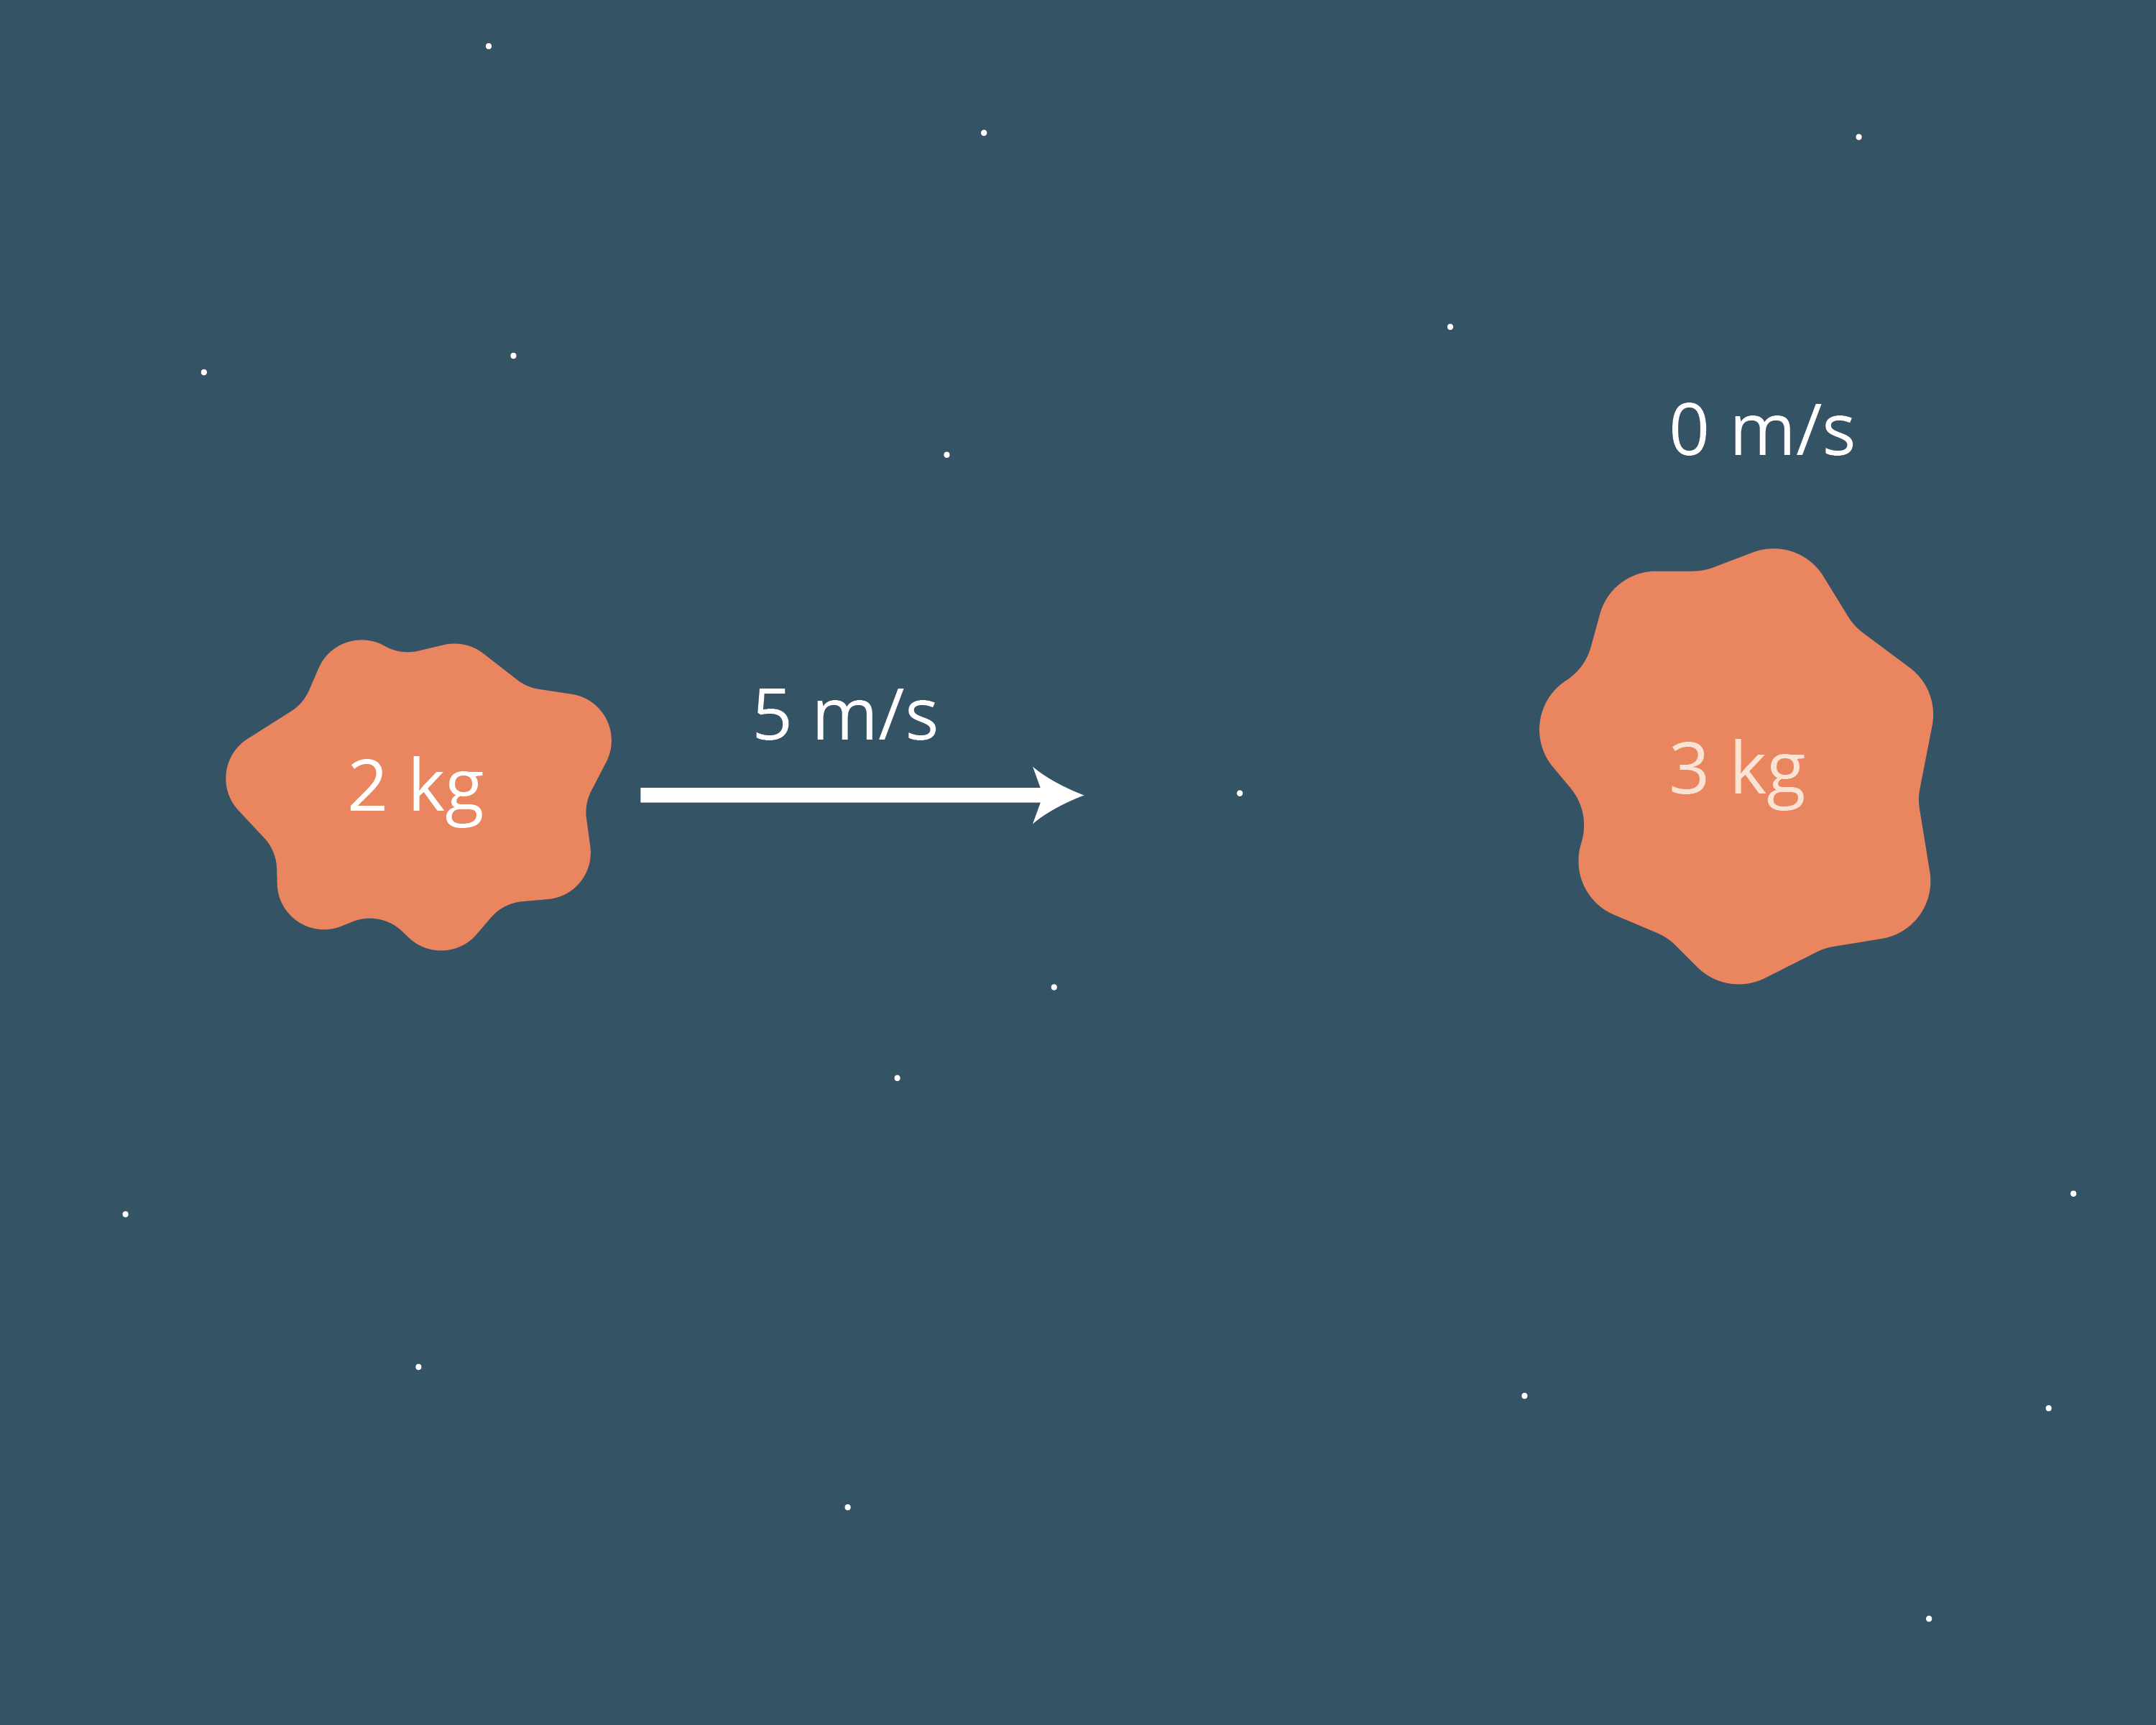
\includegraphics[width=0.4\textwidth]{putty1.png}
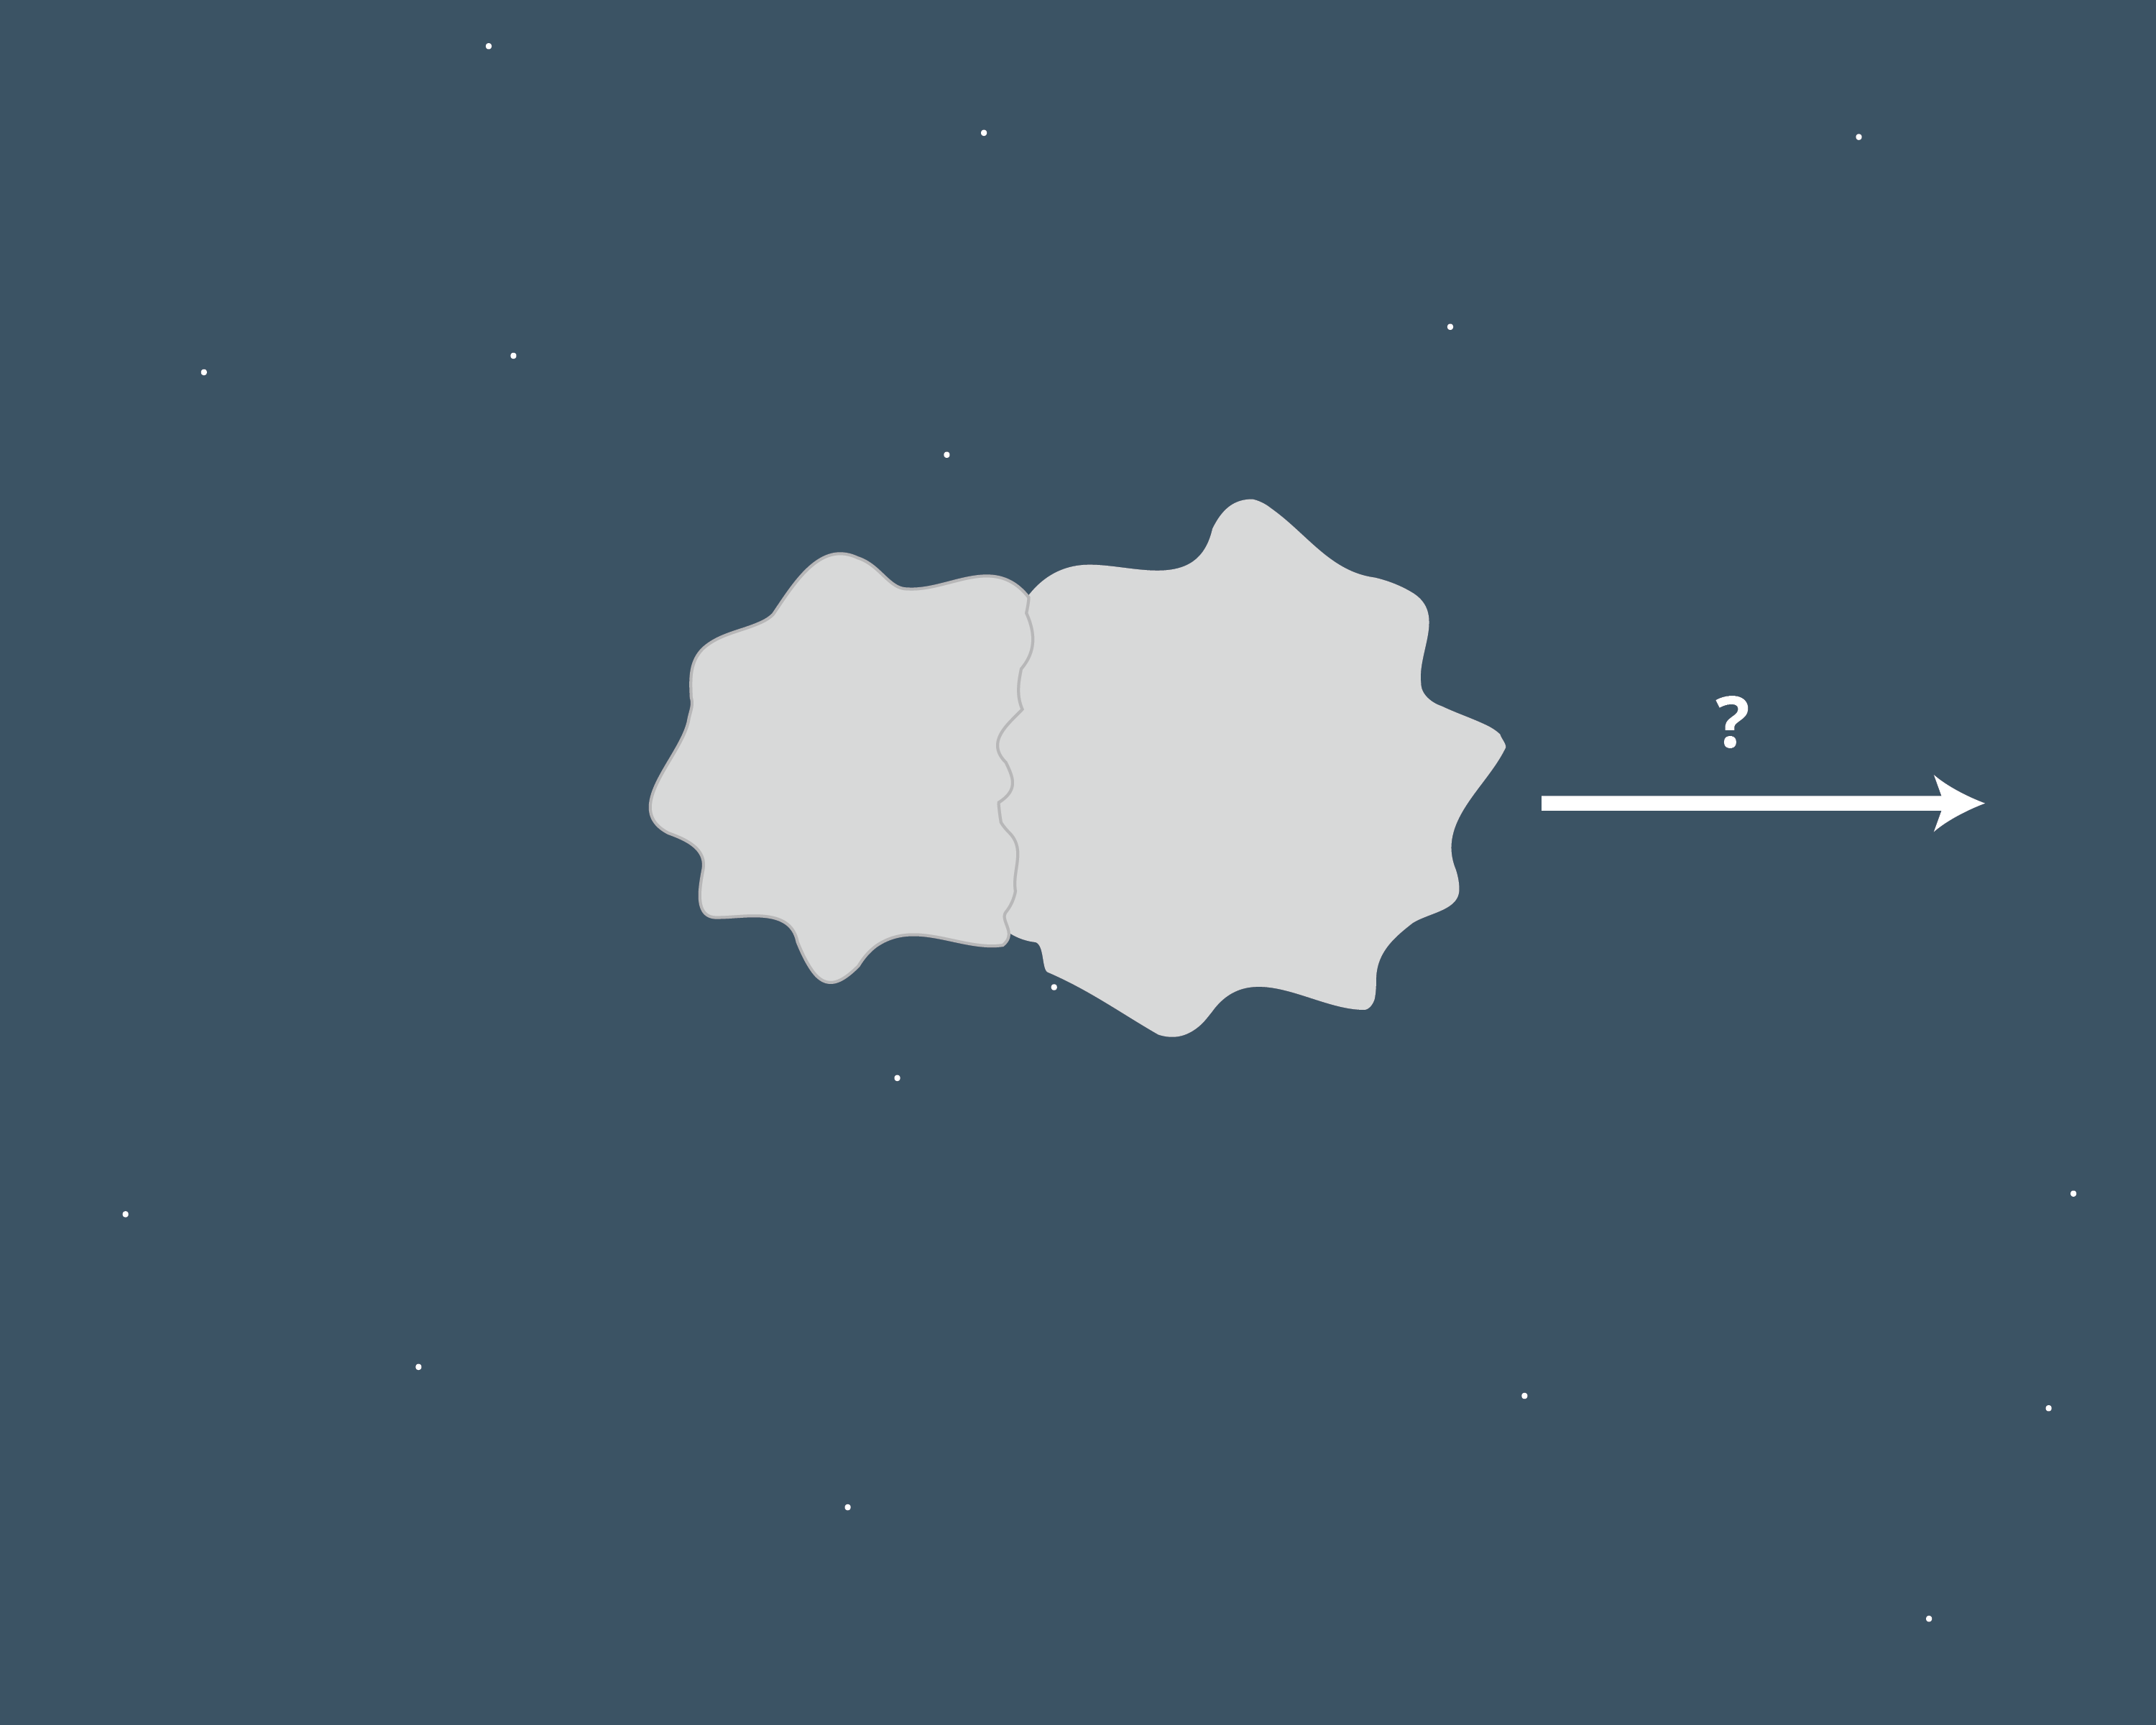
\includegraphics[width=0.4\textwidth]{putty2.png}


Every object has \newterm{momentum}.  The momentum is a vector
quantity: It points in the direction that the object is moving and has
a magnitude equal to its mass times its speed.

Given a set of objects that are interacting, we can sum all their
momentum vectors to get the total momentum.  In such a set, the total
momentum will stay constant.

So, in our example, one object has a momentum vector of magnitude of
10 kg m/s, the other has a momentum of magnitude 0.  Once they have
merged, they have a combined mass of 5 kg.  Thus, the velocity vector
must have magnitude 2 m/s and pointing in the same direction that the
first mass was moving.

\begin{Exercise}[title={Cars on Ice}, label=cars_on_ice]
A car weighing 1000 kg is going north at 12 m/s.  Another car weighing
1500 kg is going east at 16 m/s.  They both hit a patch of ice (with
zero friction) and collide.  Steel is bent and the two objects become
one.  How what is the velocity vector (direction and magnitude) of the
new object sliding across the ice?
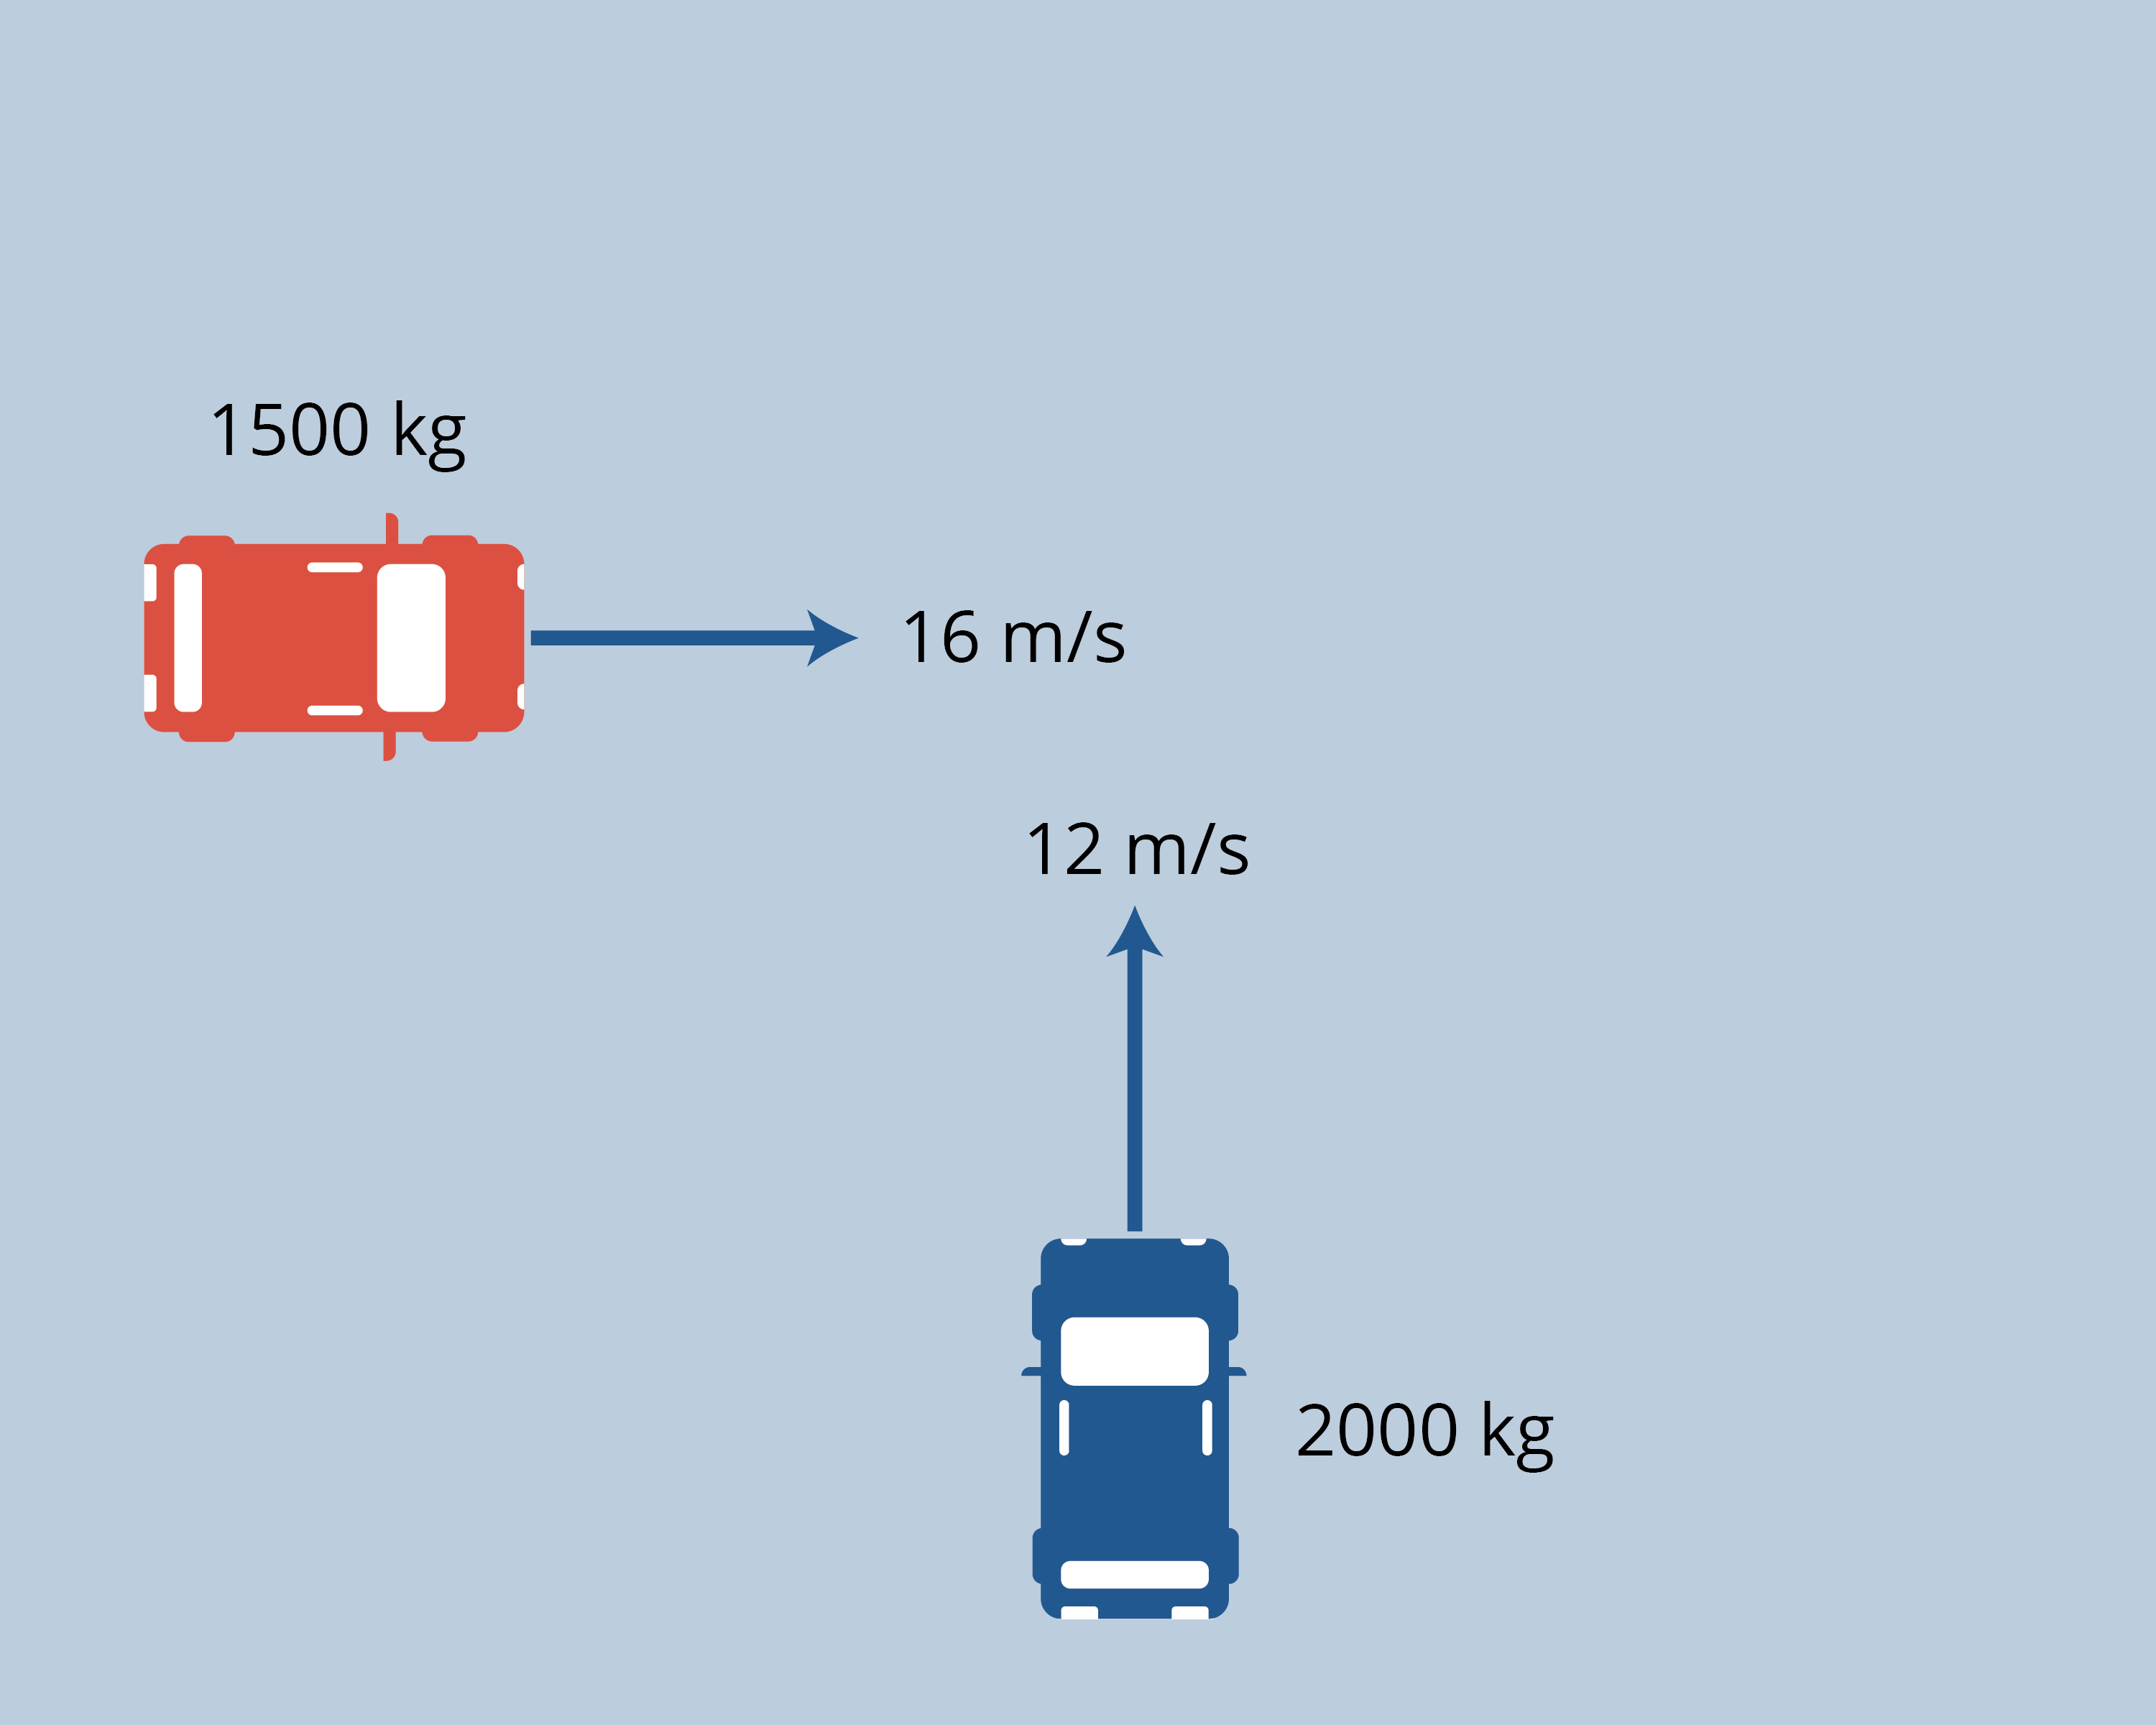
\includegraphics[width=0.4\textwidth]{icecar.png}
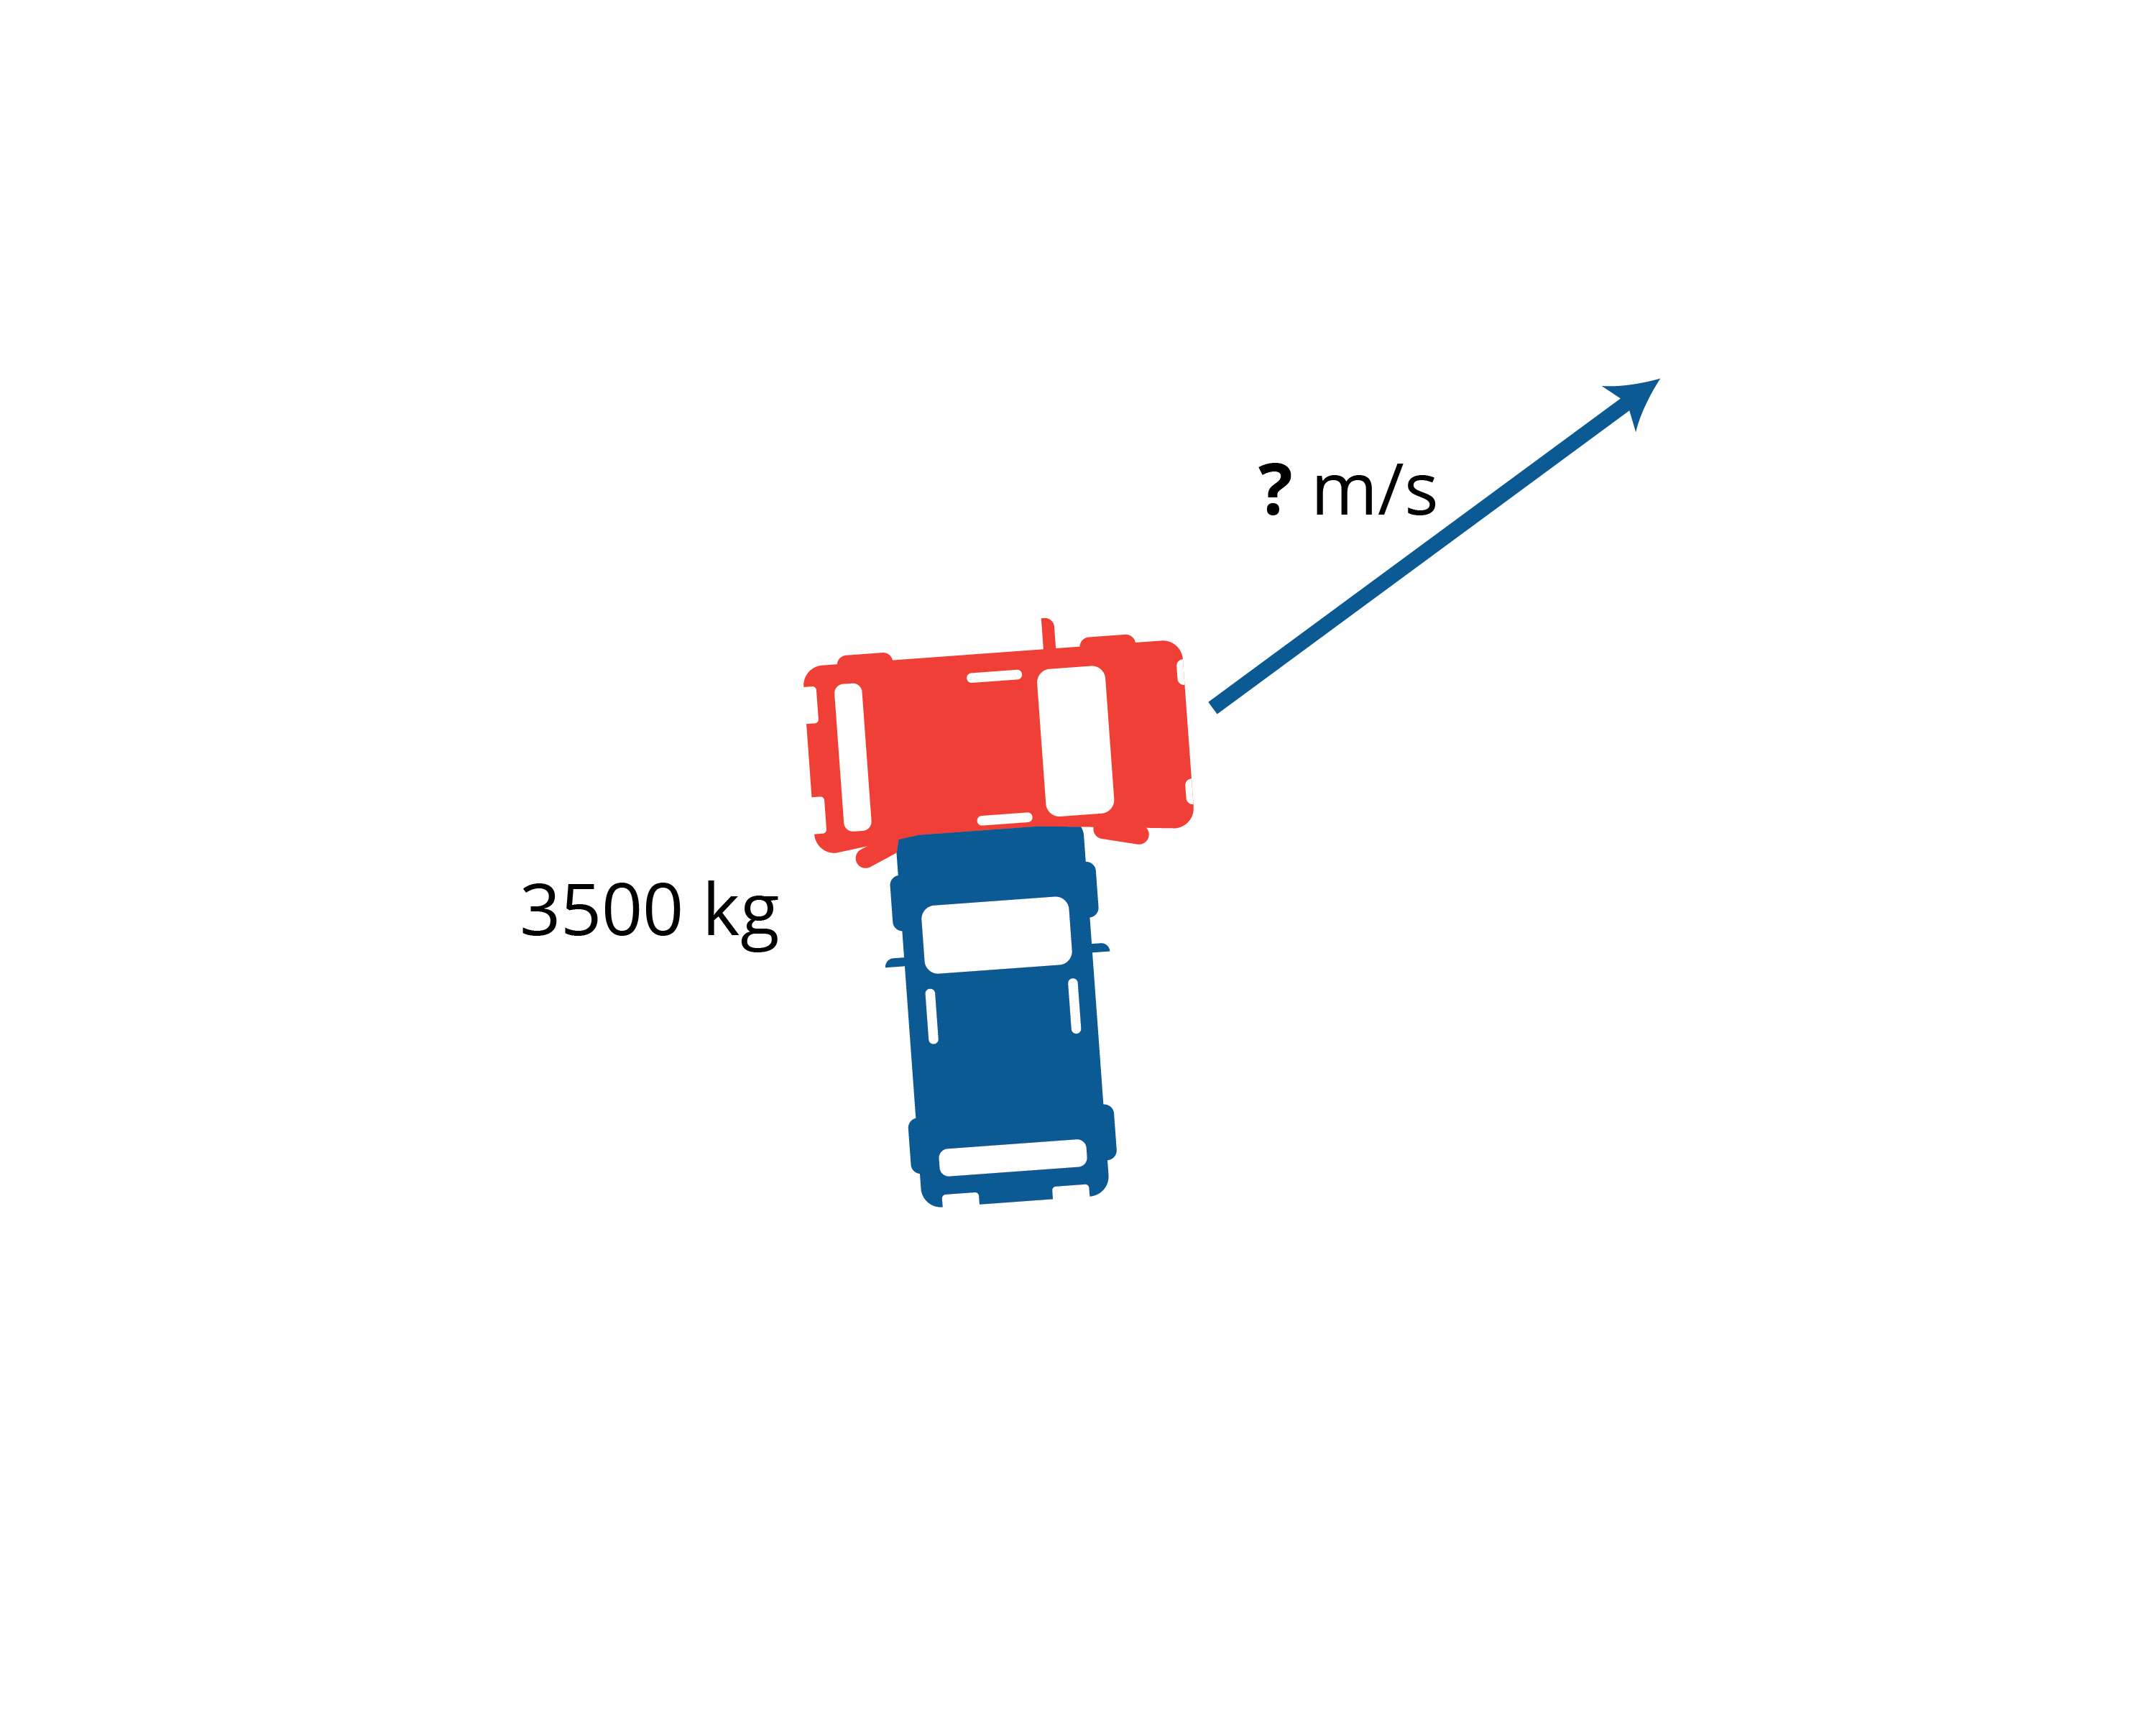
\includegraphics[width=0.4\textwidth]{icecar2.png}

\end{Exercise}
\begin{Answer}[ref=cars_on_ice]
  The momentum of the first car is 12,000 kg m/s in the north direction.

  The momentum of the second car is 24,000 kg m/s in the east direction.

  The new object will be moving northeast. What angle is the angle compared with the east?

  $$\theta = \arctan{\frac{12,000}{24,000}} \approx 0.4636 \text{ radians } \approx 26.565\text{ degrees north of east}$$

  The magnitude of the momentum of the new object is $\sqrt{12,000^2 + 24,000^2} \approx 26,833\text{ kg m/s}$

  Its new mass is 2,5000 kg.  So the speed will be $26,833/2,500 = 10.73$ m/s.
\end{Answer}


Notice that kinetic energy ($1/2 m v^2$) is \emph{not} conserved
here.  Before the collision, the moving putty block has $(1/2)(2)(5^2) = 25$
joules of kinetic energy.  Afterward, the big block has $(1/2)(5)(2^2)
= 10$ joules of kinetic energy.  What happened to the energy that was
lost? It was used up deforming the putty.

What if the blocks were marble instead of putty?  Then there would be
very little deforming, so kinetic energy \emph{and} momentum would be
conserved. The two blocks would end up having different velocity
vectors.

Let's assume for a moment that they strike each other straight on, so
there is motion in only one direction, both before and after the
collision.  Can we solve for the speeds of the first block ($v_1$) and
the second block ($v_2$)?

We end up with two equations. Conservation of momentum says:

$$2 v_1 + 3 v_2 = 10$$

Conservation of kinetic energy says:

$$(1/2)(2)(v_1^2) + (1/2)(3)(v_2^2) = 25$$

Using the first equation, we can solve for $v_1$ in terms of $v_2$:

$$v_1 = \frac{10 - 3 v_2}{2}$$

Substituting this into the second equation, we get:

$$\left(\frac{10 - 3 v_2}{2}\right)^2 + \frac{3 v_2^2}{2} = 25$$

Simplifying, we get:

$$v_2^2 - 4 v_2 + 0 = 0$$

This quadratic has two solutions: $v_2 = 0$ and $v_2 = 4$.  $v_2 = 0$
represents the situation before the collision.  Substituting in $v_2 = 4$:

$$v_1 = \frac{10 - 3(4)}{2} = -1$$

Thus, if the blocks are hard enough that kinetic energy is conserved,
after the collision, the smaller block will be heading in the opposite
direction at 1 m/s.  The larger block will be moving at 4 m/s in the
direction of the original motion.

\begin{Exercise}[title={Billiard Balls}, label=billiards]
  
A billiard ball weighing 0.4 kg and traveling at 3 m/s hits a billiard
ball (same weight) at rest. It strikes obliquely so that the ball at rest starts to
move at a 45 degree angle from the path of the ball that hit it.

Assuming all kinetic energy is conserved. How what is the velocity
vector of each ball after the collision?

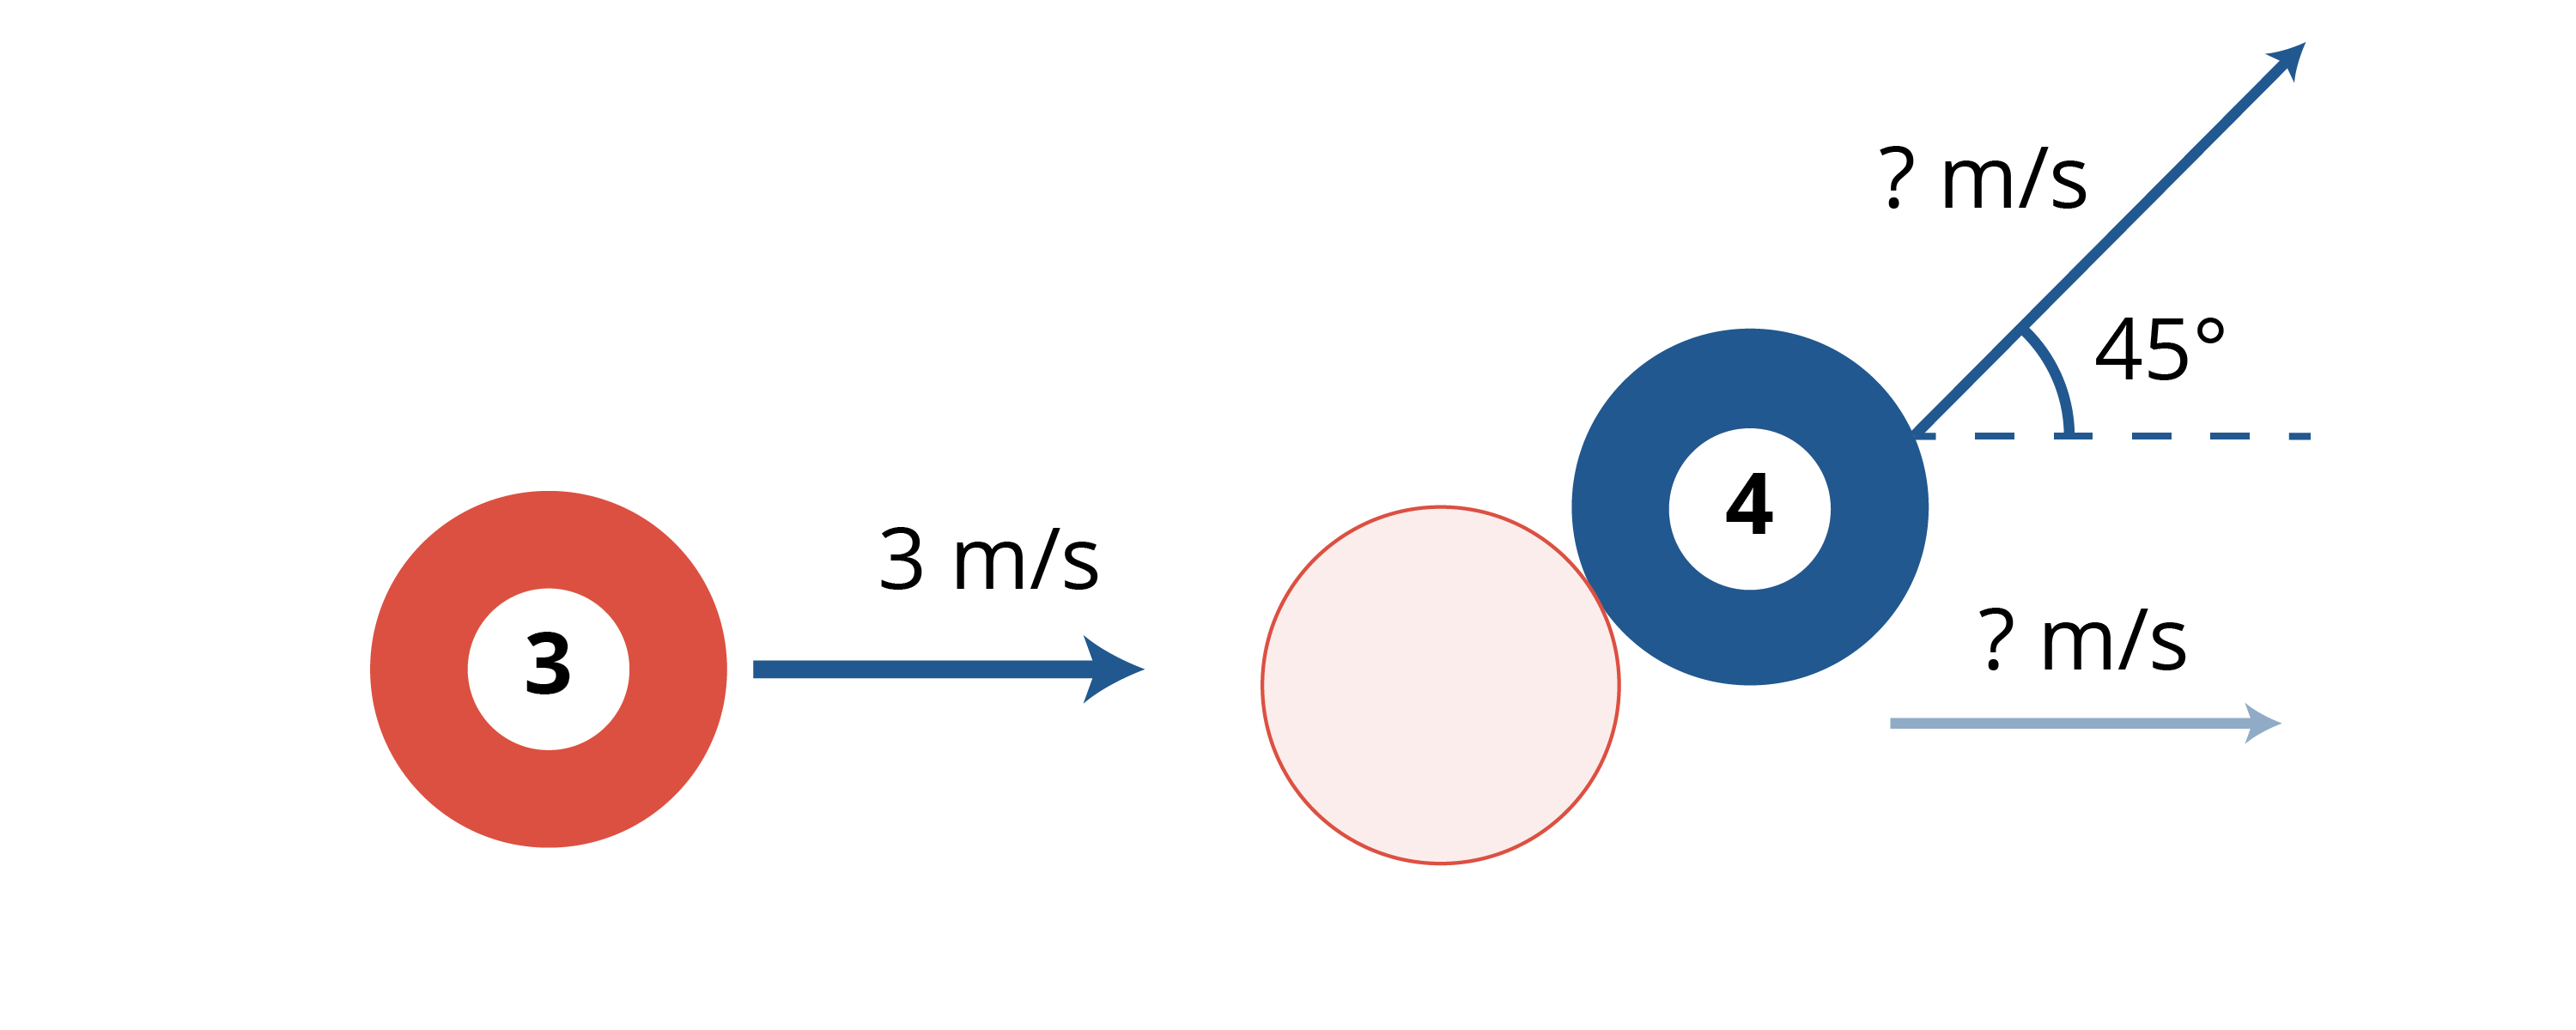
\includegraphics[width=1\textwidth]{poolball.png}

\end{Exercise}
\begin{Answer}[ref=billiards]

  The original forward momentum was 1.2 kg m/s.  The original kinetic energy is $(1/2)(0.4)(3^2)$ = 1.8 joules. 

  Let $s$ be the post-collision speed of the ball that had been at
  rest.  Let $x$ and $y$ be the forward and sideways speeds
  (post-collision) of the other ball. Conservation of kinetic energy says

  $$(1/2)(0.4)(s^2) + (1/2)(0.4)(x^2+y^2) = 1.8$$

  Forward momentum is conserved:

  $$0.4\frac{s}{\sqrt{2}} + 0.4 x = 1.2$$

  Which can be rewritten:

  $$x = 3 - \frac{s}{\sqrt{2}}$$
  
  Sideways momentum stays zero:

  $$(0.4)\frac{s}{\sqrt{2}} - 0.4 y = 0.0$$

  Which can be rewritten:

  $$y = \frac{s}{\sqrt{2}}$$

  Substituting into to the conservation of kinetic energy equation above:

  $$(1/2)(0.4)(s^2) + (1/2)(0.4)(\left(3 - \frac{s}{\sqrt{2}}\right)^2+\left(\frac{s}{\sqrt{2}}\right)^2 = 1.8$$

  Which can be rewritten:

  $$s^2 - \frac{3}{\sqrt{2}} s + 0 = 0$$

  There are two solutions to this quadratic: $s = 0$ (before collision) and $s = \frac{3}{\sqrt{2}}$. Thus,

  $$y = \frac{3}{2}$$

  and

  $$x = 3 - \frac{3}{2} = \frac{3}{2}$$

  So both balls careen off at $45^\circ$ angles at the exact same speed. 

  
\end{Answer}




\graphicspath{{../../Chapters/dot/en_US}}
\chapter{The Dot Product}
% Reference for diagrams:https://www.mathsisfun.com/algebra/vectors-dot-product.html

If you have two vectors $\textbf{u} = [u_1, u_2, \dots, u_n]$ and $\textbf{v} 
= [v_1, v_2,\dots, v_n]$, we define the \newterm{dot product} $\textbf{u} 
\cdot \textbf{v}$ as 
\begin{equation*}
     \textbf{u} \cdot \textbf{v} = (u_1 \times v_1) + (u_2 \times v_2) + \dots 
     + (u_n \times v_n)
\end{equation*} 
The output of the dot product is a \emph{scalar} quantity.


For example, 
\begin{equation*}
    [2,4, -3] \cdot [5, -1, 1] = 2 \times 5 + 4 \times -1 + -3 \times 1 = 3
\end{equation*}\index{dot product}

This may not seem like a very powerful idea, but dot products are 
\emph{incredibly} useful. The enormous GPUs (Graphics Processing Units) that 
let video games render scenes so quickly? They primarily function by computing 
huge numbers of dot products at mind-boggling speeds. 

\begin{Exercise}[title={Basic dot products}, label=dot_products]
    Compute the dot product of each pair of vectors:
    \begin{itemize}
        \item $[1, 2, 3]$, $[4, 5, -6]$
        \item $[\pi, 2\pi]$, $[2, -1]$
        \item $[0,0,0,0]$, $[10,10,10,10]$
    \end{itemize}
\end{Exercise}
\begin{Answer}[ref=dot_products]
        \begin{itemize}
            \item $[1, 2, 3] \cdot [4, 5, -6] = 4 + 10 - 18 = -4$
            \item $[\pi, 2\pi] \cdot [2, -1] = 2\pi - 2\pi = 0$
            \item $[0,0,0,0] \cdot [10,10,10,10] = 0 + 0 + 0 + 0 = 0$ 
        \end{itemize}
\end{Answer}

\section{Properties of the dot product}

Sometimes we need an easy way to say ``The vector of appropriate length is 
filled with zeros.'' We use the notation $\vec{0}$ to represent this. Then, 
for any vector $\textbf{v}$, this is true:

$$\textbf{v} \cdot \vec{0} = 0$$

The dot product is commutative:

$$\textbf{v} \cdot \textbf{u} = \textbf{u} \cdot \textbf{v}$$

The dot product of a vector with itself is its magnitude squared:

$$ \textbf{v} \cdot \textbf{v} = |\textbf{v}|^2 $$

If you have a scalar $a$, then:

    $$(\textbf{v}) \cdot (a \textbf{u}) = a (\textbf{v} \cdot \textbf{u})$$

So, if $\textbf{v}$ and $\textbf{w}$ are vectors that go in the same direction,

    $$\textbf{v} \cdot \textbf{w} = |\textbf{v}| |\textbf{w}|$$

If $\textbf{v}$ and $\textbf{w}$ are vectors that go in opposite directions,

    $$\textbf{v} \cdot \textbf{w} = -|\textbf{v}| |\textbf{w}|$$
    
If $\textbf{v}$ and $\textbf{w}$ are vectors that are perpendicular to each 
other, their dot product is zero:

  $$ \textbf{v} \cdot \textbf{w} = 0 $$

\section{Cosines and dot products}

Furthermore, dot products' interaction with cosine makes them even more useful 
is what makes them so useful: 
If you have two vectors $\textbf{v}$ and $\textbf{u}$,

$$\textbf{v} \cdot \textbf{u} = |\textbf{v}| |\textbf{u}| \cos \theta$$

where $\theta$ is the angle between them.

So, for example, if two vectors $\textbf{v}$ and $\textbf{u}$ are 
perpendicular, the angle between them is $\pi/2$. The cosine of $\pi/2$ is 0. 
The dot product of any two perpendicular vectors is always 0. In fact, if the 
dot product of two non-zero vectors is 0, the vectors \textit{must be} 
perpendicular (see figure \ref{fig:perpendicular} for an example of 
perpendicular 2-dimensional vectors). 

\begin{figure}[htbp]
    \centering
    \begin{tikzpicture}
        \begin{axis}[xmin = -2, xmax = 5, ymin = 0, ymax = 5, 
        axis lines = center]
            \draw[blue, thick, -latex] (0, 0) -- (-1, 4) 
            node[above, black, font = \scriptsize] {$\left[ -1, 4 \right]$};
            \draw[blue, thick, -latex] (0, 0) -- (4, 1) 
            node[above, black, font = \scriptsize] {$\left[ 4, 1 \right]$};
        \end{axis}
    \end{tikzpicture}
    \caption{The dot product of any two perpendicular vectors is zero.}
    \label{fig:perpendicular}
\end{figure}
% cosine is not introduced before here
If you have two non-zero vectors $\textbf{v}$ and $\textbf{u}$, you can always 
compute the angle between them:\index{vectors!angle between}

$$\theta = \arccos{ \left( \frac{\textbf{v} \cdot \textbf{u}}{|\textbf{v}| 
|\textbf{u}|} \right)}$$

Arccos is short for arccosine, or $\cos^-1$, and it is a function that is the 
inverse of cosine. Cosine takes an angle and gives back the scaled 
$x$-component of the angle. Arccosine takes the $x$-component of an angle and 
returns an angle with that $x$-component. However, there is a limit to what 
arccos can return. Let's look at cosine and its inverse, arccos (see figures 
\ref{fig:cosine} and \ref{fig:arccos}). 

\begin{figure}[htbp]
    \centering
        \begin{tikzpicture}
            \begin{axis}[xmin = -0.5, xmax = 7, ymin = -1.25, ymax = 1.25, 
            axis lines = center, xlabel = $x$, ylabel = $y$]
                \addplot[blue, thick, samples = 150, domain = -0.5:7] 
                {cos(deg(x))};
            \end{axis}
        \end{tikzpicture}
        \caption{Cosine is a function: there is exactly one output for every 
        input.}
    \label{fig:cosine}
\end{figure}

\begin{figure}[htbp]
    \centering
    \begin{tikzpicture}
            \begin{axis}[xmin = -1.25, xmax = 1.25, ymin = -0.5, ymax = 7, 
            axis lines = center, xlabel = $x$, ylabel = $y$]
                \addplot[domain = -1:1, samples = 50, blue, thick]
                {-1*rad(acos(x))};
                \addplot[domain = -1:1, samples = 100, blue, thick]
                {rad(acos(x))};
                \addplot[domain = -1:1, samples = 100, blue, thick]
                {-1*rad(acos(x)) + 6.28319};
                \draw[red, thin, dashed] (0.5, 0) -- (0.5, 7);
            \end{axis}
        \end{tikzpicture}
    \caption{Arccos is not a function: there are many angles with the same 
    $x$-component. Notice that one input value has many output values (see the 
    red dashed line).}
    \label{fig:arccos}
\end{figure}

When you use a calculator to evaluate arccos, the calculator automatically 
restricts the results to between $0$ and $\pi$. Let's look at an example of 
using the dot product to determine the angle between two vectors:

\textbf{Example}: What is the angle between $\textbf{u} = \left[ \sqrt{3}, 1 
\right]$ and $\textbf{v} = \left[ 0, -1 \right]$?

\textbf{Solution}: We know that $\textbf{u} \cdot \textbf{v} = \left| 
\textbf{u} \right| \left| \textbf{v} \right| \cos{\theta}$. Therefore, we also 
know that:
$$\cos{\theta} = \frac{\textbf{u} \cdot \textbf{v}}{\left| \textbf{u} \right| 
\left| \textbf{v} \right|}$$

First, let's compute the dot product:
$$\textbf{u} \cdot \textbf{v} = \sqrt{3} \cdot 0 + 1 \cdot -1 = -1$$

And therefore:
$$\cos{\theta} = \frac{-1}{\left| \textbf{u} \right| \left| \textbf{v} 
\right|}$$

Now, let's find the magnitudes of both vectors:
$$\left| \textbf{u} \right| = \sqrt{\left( \sqrt{3} \right)^2 + \left( 1 
\right)^2} = 2$$
$$\left| \textbf{v} \right| = \sqrt{\left( 0 \right)^2 + \left( -1 \right)^2} 
= 1$$

Substituting for the magnitudes, we find that:
$$\cos{\theta} = \frac{-1}{2 \cdot 1} = \frac{-1}{2}$$

To solve for $\theta$, we take the $\arccos$ of both sides:
$$\arccos{ \left( \cos{\theta} \right)} = \theta = \arccos{ \frac{-1}{2} }$$

What angles have a cosine of $-1 / 2$? We know that $2\pi / 3$, $4 \pi / 3$, 
$8 \pi / 3$, etc., all have a cosine of $-1 / 2$. Because the range of 
$\arccos$ is restricted to between $0$ and $\pi$, our result is:
$$\theta = \arccos{ \frac{-1}{2}} = \frac{2\pi}{3}$$.

Therefore, the angle between \textbf{u} and \textbf{v} is $2\pi / 3$ (or $120^{
\circ}$). 

\begin{Exercise}[title={Using dot products}, label=cos_dot_products]
    What is the angle between these each pair of vectors:
    \begin{itemize}
        \item $[1, 0]$, $[0, 1]$
        \item $[3,4]$, $[4,3]$
        \item $[ 2, -1, 2 ]$, $[-1, 2, -2 ]$
        \item $[-5, 0, -1]$, $[2, 3, -4]$
    \end{itemize}
\end{Exercise}
\begin{Answer}[ref=cos_dot_products]
        \begin{itemize}
            \item $[1,0] \cdot [0,1] = 0$.  The angle must be $\pi/2$.
            \item $[3,4] \cdot [4, 3] = 24$. $|[3,4]| |[4,3]| \cos(\theta) = 24$. 
            $\cos(\theta) = \frac{24}{(5)(5)}$. $\theta = \arccos(\frac{24}{25}) 
            \approx 0.284 \text{ radians}$.
            \item $[2, -1, 2] \cdot [-1, 2, -2] = 4 - 2 - 4 = -2$. $|[2, -1, 2]| = \sqrt{4 + 1 + 4} = \sqrt{9} = 3$. $|[-1, 2, -2]| = \sqrt{1 + 4 + 4} = \sqrt{9} = 3$. $3(3) \cos{\theta} = -2$. $\theta = \arccos{ (-2 / 9)} \approx 1.795 \text{ radians}$.
            \item $[ -5, 0, -1] \cdot [2, 3, -4] = -10 + 0 + 4 = -6$. $|[-5, 0, 1]| = \sqrt{25 + 0 + 1} = \sqrt{26}$. $|[2, 3, -4]| = \sqrt{4 + 9 + 16} = \sqrt{29}$. $\sqrt{26} (\sqrt{29}) \cos{\theta} = -6$. $\theta = \arccos{(\frac{-6}{\sqrt{26}\sqrt{29}})} \approx 1.791 \text{ radians}$.
        \end{itemize}
\end{Answer}

\section{Dot products in Python}

NumPy will let you do dot products using the the symbol @.  Open \filename{first\_vectors.py} 
and add the following to the end of the script:

\begin{Verbatim}
    # Take the dot product
    d = v @ u
    print("v @ u =", d)
    
    # Get the angle between the vectors
    a = np.arccos(d / (mv * mu))
    print(f"The angle between u and v is {a * 180 / np.pi:.2f} degrees")    
\end{Verbatim}

When you run it you should get:
\begin{Verbatim}
v @ u = 4
The angle between u and v is 78.55 degrees
\end{Verbatim}

\section{Work and Power}
%diagram here
Earlier, we mentioned that mechanical work is the product of the 
force you apply to something and the amount it moves. For example, if you 
push a train with a force of 10 newtons as it moves 5 meters, you have done 50 joules of work.

What if you try to push the train sideways? It moves down the track 5 meters, 
but you push it as if you were trying to derail it --- perpendicular to its motion.  
You have done no work, because the train didn't move at all in the direction you were pushing.

% 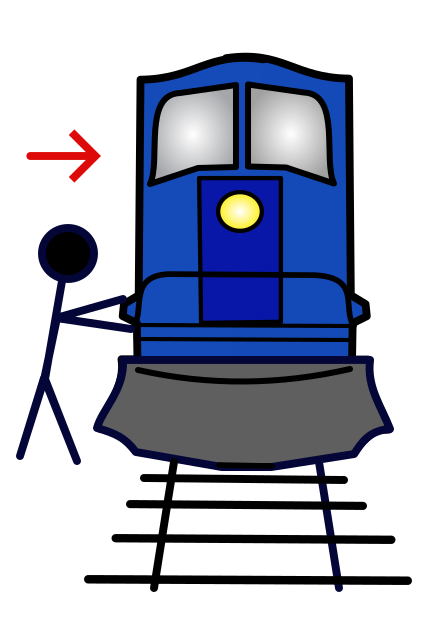
\includegraphics[width=0.8\textwidth]{train.png}


Now that you know about dot products: The work you do is the dot
product of the force vector you apply and the displacement vector of the train. (The displacement
vector is the vector that tells how the train moved while you pushed it.) \index{work}

Similarly, we mentioned that power is the product of the force you apply and the velocity of the
mass you are applying it to. It is actually the dot product of the force vector and the velocity vector.\index{power}

For example, if you are pushing a sled with a force of 10 newtons and it is moving 2 meters per second, 
but your push is 20 degrees off, you aren't transferring 20 watts of power to the sled.  
You are transferring $10 \times 2 \times \cos(20 \text{ degrees}) \approx 18.8$ watts of power.
%add ramps and sin

\graphicspath{{../../Chapters/functions/en_US}}
\chapter{Functions and Their Graphs}

Functions are a major part of science, engineering, and math. You can think of a function as a machine: you put something into the
machine, it processes it, and out comes something else: a product. Just as we
often use the variable $x$ to stand in for a number, we often use the
variable $f$ to stand in for a function. $f(x)$ is said as ``f of x``.
% One of my teachers told me half of understanding math is understanding mathmaticions are just lazy, maybe a good add in somewhere

For example, we might ask, ``Let the function $f$ be defined like this:

\begin{equation*}
f(x) = -5x^2 + 12x + 2
\end{equation*}

What is the value of $f(3)$, said as ``f of 3``?

You would run the number 3 through ``the machine'': $-5(3^2) + 12(3) + 2 = -7$. The answer would be ``$f(3)$ is $7$''.

However, some functions are not defined for every possible input. For example:

\begin{equation*}
  f(x) = \frac{1}{x}
\end{equation*}

  This is defined for any $x$ except 0, because you can't divide 1 by 0. The set of values that a function can process is called its \textit{domain}, and resulting output values are called the range.
  It is important to note that functions have only one \emph{output} for each \emph{input}. However, multiple inputs can have the same output. 
  A relationship where one input can result in the more than one output is not a function, but a relation. This can be proven by the \hyperref[sec:vertical]{vertical line test}.
% some good images could be found here: https://www.ck12.org/book/ck-12-algebra-i-honors/section/3.1/ 

\begin{Exercise}[title={Domain of a function}, label=function_domain]

  Let the function $f$ be given by $f(x) = \sqrt{x - 3}$.  What is its domain?

\end{Exercise}
\begin{Answer}[ref=function_domain]
  You can only take the square root of nonnegative numbers, so the
  function is only defined when $x - 3 \geq 0$.  Thus, the domain is
  all real numbers greater than or equal to 3.
\end{Answer}

\section{Graphs of Functions}

If you have a function, $f$, its graph is the set of pairs $(x, y)$
such that $y = f(x)$.  We usually draw a picture of this set, called a \textit{graph}. 
The graph not only includes the picture, but also the values of x and y used to create it.

Here is the graph of the function $f(x) = -5x^2 + 12x + 2$:

\begin{tikzpicture}
    \begin{axis}[
        xmin=-1,xmax=3.5,
        ymin=-10,ymax=11,
        axis x line=middle,
        axis y line=middle,
        axis line style=<->,
        xlabel={$x$},
        ylabel={$y$},
        ]
        \addplot[no marks,sdkblue,<->] expression[domain=-0.7:3.05,samples=100]{(-5)*(x^2) + (12 * x) + 2}; 
    \end{axis}
\end{tikzpicture}

(Note that this is just part of the graph; it goes infinitely in both
directions. Remember your vectors!)

Here is the graph of the function $f(x) = \frac{1}{x}$:

\begin{tikzpicture}
    \begin{axis}[
        xmin=-7,xmax=7,
        ymin=-7,ymax=7,
        axis x line=middle,
        axis y line=middle,
        axis line style=<->,
        xlabel={$x$},
        ylabel={$y$},
        ]
        \addplot[no marks,sdkblue,<->] expression[domain=-6.5:-0.15,samples=100]{1/x}; 
        \addplot[no marks,sdkblue,<->] expression[domain=0.15:6.5,samples=100]{1/x}; 
    \end{axis}
\end{tikzpicture}
To draw a graph, take each x value (usually in increments of 1) and determine its corresponding y value. 
Then, plot those points on a graph, using the origin as the starting point. 
% do we assume students know how to graph?
\begin{Exercise}[title={Draw a graph}, label=draw_graph]

  Let the function $f$ be given by $f(x) = -3x + 3$. Sketch its graph.
% More space needed in exercise box
\end{Exercise}
\begin{Answer}[ref=draw_graph]

  The graph of this function is a line, its slope is -3, and it intersects the y axis at $(0, 3)$.

\begin{tikzpicture}
    \begin{axis}[
        xmin=-1,xmax=3,
        ymin=-7,ymax=7,
        xtick={1},
        ytick={3},
        axis x line=middle,
        axis y line=middle,
        axis line style=<->,
        xlabel={$x$},
        ylabel={$y$},
        ]
        \addplot[no marks,sdkblue,<->] expression[domain=-0.75:2.74,samples=100]{-3 * x + 3}; 
    \end{axis}
\end{tikzpicture}
  
  
\end{Answer}


\section{Can this be expressed as a function?}
\label{sec:vertical}

Note that not all sets can be expressed as graphs of functions.  For
example, here is the set of points $(x,y)$ such that $x^2 + y^2 = 9$:

\begin{tikzpicture}
    \begin{axis}[
        xmin=-3.5,xmax=3.5,
        ymin=-3.5,ymax=3.5,
        ytick={-3,-2,-1,0,1,2,3},
        axis x line=middle,
        axis y line=middle,
        axis line style=<->,
        xlabel={$x$},
        ylabel={$y$},
        ]
        \addplot[no marks,sdkblue] expression[domain=-3:3,samples=100]{sqrt(9 - x^2)}; 
        \addplot[no marks,sdkblue] expression[domain=-3:3,samples=100]{-1 * sqrt(9 - x^2)}; 
    \end{axis}
\end{tikzpicture}

This cannot be the graph of a function, because what would $f(0)$ be? 3
or -3?  This set fails what we call ``the vertical line test'': If any
vertical line contains more than one point from the set, it isn't the graph
of a function.  For example, the vertical line $x = 2$ would cross the graph twice:
\begin{center}
  
  \begin{tikzpicture}
    \begin{axis}[
      xmin=-3.5,xmax=3.5,
      ymin=-3.5,ymax=3.5,
      ytick={-3,-2,-1,0,1,2,3},
      axis x line=middle,
      axis y line=middle,
      axis line style=<->,
      xlabel={$x$},
      ylabel={$y$},
      ]
      \addplot[no marks,sdkblue] expression[domain=-3:3,samples=100]{sqrt(9 - x^2)}; 
      \addplot[no marks,sdkblue] expression[domain=-3:3,samples=100]{-1 * sqrt(9 - x^2)};
      \addplot [thick, dashed] coordinates {(2,-2.5)(2,2.5)};
      
    \end{axis}
    
  \end{tikzpicture}
\end{center}
%might be a good place to talk about even vs odd functions
\index{vertical line test}

\section{Inverses}

Some functions have inverse functions. If a function $f$ is a machine that turns
number $x$ into $y$, the inverse (usually denoted $f^{-1}$) is the machine that turns $y$ back
into $x$.

For example, let $f(x) = 5x + 1$. Its inverse is
$f^{-1}(x) = (x - 1)/5$. (Spot check it: $f(3) = 16$ and $f^{-1}(16) = 3$)

Does the function $f(x) = x^3$ have an inverse? Yes, $f^{-1}(x) =
\sqrt[3]{x}$. Let's plot the function (solid line) and its inverse (dashed):

\begin{tikzpicture}
    \begin{axis}[
        xmin=-3.5,xmax=3.5,
        ymin=-3.5,ymax=3.5,
        ytick={-3,-2,-1,0,1,2,3},
        axis x line=middle,
        axis y line=middle,
        axis line style=<->,
        xlabel={$x$},
        ylabel={$y$},
        ]
        \addplot[no marks,sdkblue] expression[domain=-3:3,samples=100]{x^3}; 
        \addplot[no marks,sdkblue,dashed] expression[domain=0:3,samples=100]{x^(1/3)}; 
        \addplot[no marks,sdkblue,dashed] expression[domain=-3:0,samples=100]{-1 * (-1 * x)^(1/3)}; 
    \end{axis}
\end{tikzpicture}

The inverse is the same as the function, just with its axes swapped.
The inverse function is \emph{reflected} across the line $y=x$. \index{reflections}
This tells us how to solve for an inverse: We swap $x$ and $y$ and
solve for $y$.

For example, if you are given the function $f(x) = 5x + 1$, its graph
is all $(x,y)$ such that $y = 5x + 1$.  The graph of its inverse is
all $(x, y)$, such that $x = 5y + 1$. Solving for $y$ gives you $y = (x -
1)/5$. So we can say that $f^{-1}(x) = (x - 1)/5$, QED.

Not every function has an inverse.  For example, $f(x) = x^2$.  Note
that $f(2) = f(-2) = 4$.  What would $f^{-1}(4)$ be? 2 or -2?  This
implies the ``horizontal line test'': If any horizontal line contains
more than one point of a function's graph, that function has no
inverse. If a function passes the horizontal line test, it is called 
"one-to-one", meaning there is exactly one $x$ that gives each $y$. \\
\index{horizontal line test}
\begin{center}
  \begin{tikzpicture}
    \begin{axis}[
      xmin=-3.5,xmax=3.5,
      ymin=-1, ymax=6,
      ytick={-1,0,1,2,3,4,5,6},
      axis x line=middle,
      axis y line=middle,
      axis line style=<->,
      xlabel={$x$},
      ylabel={$y$},
      ]
      \addplot[no marks,sdkblue] expression[domain=-3:3,samples=100]{x^2};
      \addplot [thick, dashed] coordinates {(-3,4)(3,4)};
    \end{axis}
  \end{tikzpicture}
\end{center}

In some problems, you need an inverse, but you don't need the
whole domain, so you trim the domain to a set you can define an
inverse on. This allow you to make claims such as ``If we restrict the domain to
the nonnegative numbers, the function $f(x) = x^2 - 5$ has an inverse:
$f^{-1}(x) =\sqrt{x + 5}$.

This raises the question: What is the domain of the inverse function $f^{-1}$?

If we let $X$ be the domain of $f$, we can run every member of $X$
through ``the machine'' and gather them in a set on the other
side. This set would be the \textit{image} of the $f$ "machine". (This is the \textit{range} of $f$.)

What is the image of $f(x) = x^2 - 5$? It is the set of all real
numbers greater than or equal to -5. We write this:

\begin{equation*}
  \{ x \in {\rm I\!R} | x \geq -5 \}
  \end{equation*}

Now we can say: \textbf{The range (or image) of the function is the domain
  of the inverse function.}

In inverse functions, the domain and range get swapped: 
the domain of the function is the range of the inverse function, and visa versa.
In our example, we can use any number greater
than or equal to -5 as input into the inverse function.

\begin{tikzpicture}
    \begin{axis}[
        xmin=-5.5,xmax=7.5,
        ymin=-6, ymax=5,
        xtick={-3, 2},
        ytick={-5, 1},
        axis x line=middle,
        axis y line=middle,
        axis line style=<->,
        ]
      \addplot[no marks,sdkblue, ->] expression[domain=0:3,samples=100]{x^2 - 5} node[right] {$y = x^2 - 5$};
      \addplot [thick, dashed, red, ->] coordinates {(-0.05,-5)(-0.05,4.5)}
      node [draw, red, left, align=left, yshift=-0.6cm, xshift=-0.1cm] {image of $f$ \textit{or}\\ domain of $f^{-1}$};
      \addplot [thick, dashed, blue, ->] coordinates {(-0,-5.1)(6.75,-5.1)}
      node [draw, align=left, above, blue, yshift=0.1cm, xshift=-1.3cm] {domain of $f$ \textit{or}\\image of $f^{-1}$};
    \end{axis}
\end{tikzpicture}


\begin{Exercise}[title={Find the inverse}, label=simple_inverse]

  Let $f(x) = (x - 3)^2 + 2$.  Sketch the graph.

  Using all the real numbers as a domain, does this function have an inverse?

  How would you restrict the domain to make the function invertible?

  What is the inverse of that restricted function?

  What is the domain of the inverse?

\end{Exercise}
\begin{Answer}[ref=simple_inverse]

  This graph is the graph of $y = x^2$ that has been moved to the right by three units and up two units:
 
\begin{tikzpicture}
    \begin{axis}[
        xmin=-1,xmax=7,
        ymin=-1,ymax=7,
        xtick={3, 6},
        ytick={2, 4},
        axis x line=middle,
        axis y line=middle,
        axis line style=<->,
        xlabel={$x$},
        ylabel={$y$},
        ]
      \addplot[no marks,sdkblue,<->] expression[domain=-2.5:6.5,samples=100]{(x - 3)^2 + 2};
      \addplot[dashed] coordinates {(-1, 2)(4,2)};
      \addplot[dashed] coordinates {(3, -1)(3, 3)};
    \end{axis}
\end{tikzpicture}

To prevent any horizontal line from containing more than one point of
the graph, you would need to use the left or the right side --- either
$\{x \in {\rm I\!R}  | x \leq 3\}$ or $\{x {\rm I\!R}| x \geq 3\}$. Most people will choose the
right side; the rest of the solution will assume that you did too.

To find the inverse we swap $x$ and $y$: $x = (y -3)^2 + 2$

Next, we solve for $y$ to get the inverse: $y = \sqrt{x - 2} + 3$

You can take the square root of nonnegative numbers. So the function
$f^{-1}(x) = \sqrt{x - 2} + 3$ is defined whenever $x$ is greater than
or equal to 2.

\end{Answer}

\begin{Exercise}[label=invfunc1]
A function is given by a table of values, a graph, or a written description. 
Determine whether it is one-to-one. 
	\begin{enumerate}
	\item
	\begin{tabular}{|c|c|c|c|c|c|c|}\hline
	$x$ & 1 & 2 & 3 & 4 & 5 & 6\\
	\hline
	$f(x)$ & 1.5 & 2.0 & 3.6 & 5.3 & 2.8 & 2.0\\
	\hline	
	\end{tabular}
	\item
	\begin{tabular}{|c|c|c|c|c|c|c|}\hline
	$x$ & 1 & 2 & 3 & 4 & 5 & 6\\
	\hline
	$f(x)$ & 1.0 & 1.9 & 2.8 & 3.5 & 3.1 & 2.9\\
	\hline	
	\end{tabular}
	\item
	\begin{tikzpicture}[scale=0.5]
		\begin{axis}
		[xmin=-2, xmax=2, xlabel=$x$,
		ymin=-0.5, ymax=4, ylabel=$y$,
		axis lines = center, ticks=none]
		\addplot[blue, thick, samples=100]{e^(-1*x^2)+1};
		\end{axis}
	\end{tikzpicture}
	\item
	\begin{tikzpicture}[scale=0.5]
		\begin{axis}
		[xmin=-1, xmax=3, xlabel=$x$,
		ymin=-2, ymax=2, ylabel=$y$,
		axis lines = center, ticks=none]
		\addplot[blue, thick, samples=100]{-ln(x+1)};
		\end{axis}
	\end{tikzpicture}
	\item $f(t)$ is the height of a football $t$ seconds after kickoff
	\item $v(t)$ is the velocity of a dropped object
	\end{enumerate}
\end{Exercise}

\begin{Answer}[ref=invfunc1]
	\begin{enumerate}
	\item This function is not one-to-one. From $x=3$ to $x=4$, the 
	function increases from 3.6 to 5.3, which means it must pass through 
	$f(x_1)=4.0$. From $x=4$ to $x=5$, the function decreases from 5.3 to 
	2.8, which means it must pass through $f(x_2) = 4.0$ again. 
	\item This function is not one-to-one by a similar argument in the 
	above solution
	\item This function is not one-to-one, because it fails the horizontal 
	line test
	\item This function is one-to-one, because it passes the horizontal 
	line test
	\item $f(t)$ would not be one-to-one because the football must pass 
	through each height (except the peak height) both on the way up and 
	on the way back down
	\item $v(t)$ would be one-to-one because a falling object only speeds 
	up. Therefore, every time has a unique speed. 
	\end{enumerate}
\end{Answer}

\section{Graphing Calculators}

One really easy way to understand your function better is to use a graphing
calculator. Desmos is a great, free online graphing calculator. 

In a web browser, go to Desmos: \url{https://www.desmos.com/calculator}

In the field on the left, enter the function $y = x^2 - x - 6$. (For
the exponent, just prefix it with a caret symbol: ``x\^{}2''.)

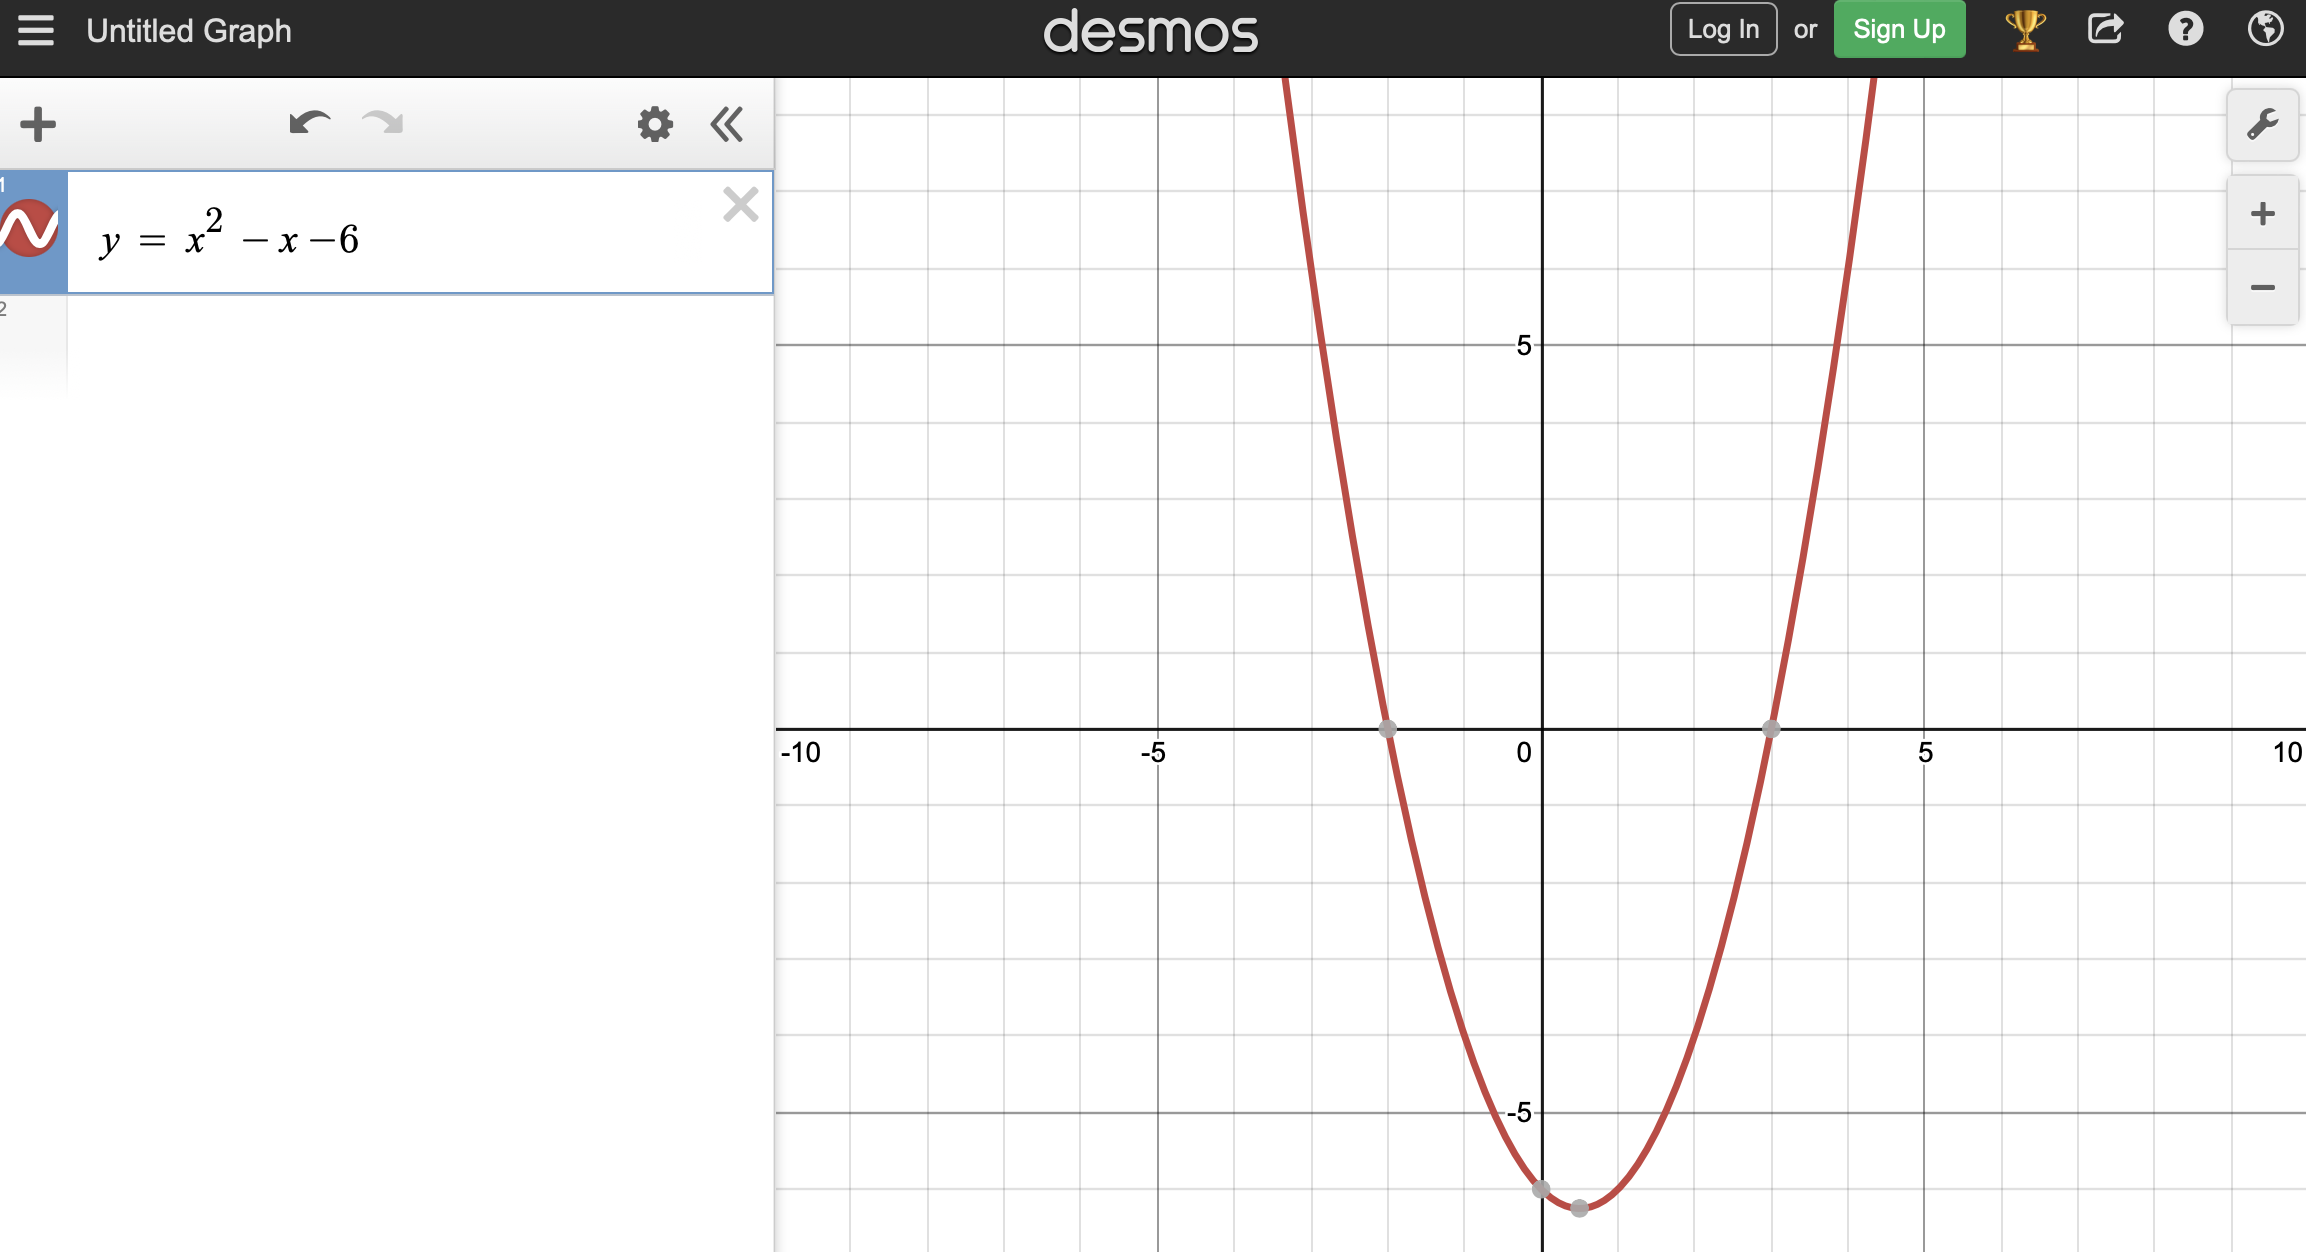
\includegraphics[width=0.85\textwidth]{Desmos.png}

\section{Even and Odd Functions}


\subsection{Even Functions}

An even function is symmetric about the y-axis. That means if you fold the graph along the y-axis, both sides will match perfectly. Note that the input value yields the same output regardless of whether the input value is positive or negative. 


\begin{mdframed}[style=important, frametitle={Even Functions}]

A function \( f(x) \) is even if  
\[
f(-x) = f(x)
\]  
for all \( x \) in its domain.
\end{mdframed}
Examples:
\begin{itemize}
  \item \( f(x) = x^2 \)  
  \item \( f(x) = \cos(x) \)  
  \item any \( f(x) = x^n \) where \( n \) is an even number
  \item \( f(x) = |x| \)
\end{itemize}

On a graph, a function will be a mirror image across the y-axis.

\subsection{Odd Functions}

An odd function is symmetric about the origin. That means if you rotate the graph $180^\circ$ about the origin, it lands on itself. Algebraically, when you input a value $k$, you get some output $n$; if you negate that input as $-k$, the output is also negated resulting in $-n$.


\begin{mdframed}[style=important, frametitle={Odd Functions}]

A function \( f(x) \) is odd if  
\[
f(-x) = -f(x)
\]
for all \( x \) in its domain.

Equivallently, 

\[ f(x) + f(-x) = 0 \]
for all \( x \) in its domain.
\end{mdframed}

\begin{itemize}

  \item \( f(x) = x^3 \)  
  \item \( f(x) = \sin(x) \)  
  \item \( f(x) = \tan(x) \)  
  \item any \( f(x) = x^n \) where \( n \) is an odd number
\end{itemize} 

On a graph, rotating the graph $180^\circ$ about the origin will yield the same graph.
\subsection{Neither Even Nor Odd}
Some functions are neither even nor odd. 

For example, \( f(x) = x^3 + 1 \) does not satisfy either condition.
% FIXME do we need to talk about end behavior, limits, symetry, etc
\graphicspath{{../../Chapters/falling_bodies/en_US}}
\chapter{Falling Bodies}

Because of gravity, if you throw a hammer straight up in the air, from
the moment it leaves your hand until it hits the ground, it is
accelerating toward the center of the earth at a constant rate.

\emph{Acceleration} can be defined as change in velocity. If the hammer leaves your
hand with a velocity of 12 meters per second upward, one second later
it will be rising, and its velocity will have slowed to 2.2 meters per
second. One second after that, the hammer will be falling at a rate of
7.6 meters per second. Every second the hammer's velocity is changing by
9.8 meters per second, and that change is always toward the center of
the earth. When the hammer is going up, gravity is slowing it down by
9.8 meters per second, each second it is in the air.  When the hammer is coming down,
gravity is speeding it up by 9.8 meters per second.\index{acceleration}
% Connect to vectors
\includegraphics[width=1\textwidth]{hammerFall.png}


\includegraphics[width=1\textwidth]{hammerTime.png}

Acceleration due to gravity on earth is a constant negative 9.8 meters per second per second:
\begin{equation*}
a = -9.8   
\end{equation*}
(Why is it negative? We are talking about height, which increases as
you go away from the center of the earth. Acceleration is changing the
velocity in the opposite direction.)

\section{Calculating the Velocity}

Given that the acceleration is constant, it makes sense that the
velocity is a straight line. Assuming once again that the hammer
leaves your hand at 12 meters per second, then the upwards velocity at
time $t$ is given by:
\begin{equation*}
  v = 12 - 9.8t
\end{equation*}

Note that the velocity of the hammer is being given as a function. Here is its graph:

\begin{tikzpicture}
    \begin{axis}[
        xmin=-0.25,xmax=2.75,
        ymin=-13,ymax=13,
        axis x line=middle,
        axis y line=middle,
        axis line style=<->,
        xlabel={$t$},
        ylabel={$v$},
        ]
        \addplot[no marks,sdkblue] expression[domain=0:2.25,samples=100]{x * (-9.8) + 12} node[left] {$12 - 9.8t$}; 
    \end{axis}
\end{tikzpicture}

\begin{Exercise}[title={When is the apex of flight?}, label=vapex]
  Given the hammer's velocity is given by $12 - 9.8t$, at what time (in seconds)
  does it stop rising and begin to fall?
\end{Exercise}
\begin{Answer}[ref=vapex]
  Solve for when the velocity is zero.

  $t = \frac{12}{9.8} = 1.22$ seconds after release.
\end{Answer}

At this point, we need to acknowledge air resistance. Gravity
is not the only force on the hammer; as it travels through the air,
the air tries to slow it down. This force is called \emph{air resistance},
and for a large, fast-moving object (like an airplane) it is GIGANTIC force. For a
dense object (like a hammer) moving at a slow speed (what you generate
with your hand), air resistance doesn't significantly affect acceleration.
% Relate to f=ma

\section{Calculating Position}

If you let go of the hammer when it is 2 meters
above the ground, the height of the hammer is given by:
\begin{equation*}
  p = -\frac{9.8}{2}t^2 + 12t + 2
\end{equation*}

Here is a graph of this function:

\begin{tikzpicture}
    \begin{axis}[
        xmin=-1.2,xmax=3.5,
        ymin=-13,ymax=13,
        axis x line=middle,
        axis y line=middle,
        axis line style=<->,
        xlabel={$t$},
        ylabel={$p$},
      ]
      \addplot[no marks,sdkblue,dashed,<-] expression [domain=-0.7:0,samples=100] {(-4.9)*(x^2) + 12 * x + 2};
      \addplot[no marks,sdkblue] expression [domain=0:2.58,samples=100] {(-4.9)*(x^2) + 12 * x + 2};
      \addplot[no marks,sdkblue,dashed,->] expression [domain=2.58:3,samples=100] {(-4.9)*(x^2) + 12 * x + 2};
    \end{axis}
\end{tikzpicture}


How do we know? \textbf{The change in position between time
  $0$ and any time $t$ is equal to the area under the velocity graph
  between $x = 0$ and $x = t$.}

Let's use the velocity graph to figure out how much the position has
changed in the first second of the hammer's flight. Here's the
velocity graph with the area under the graph for the first second filled
in:

\usepgfplotslibrary{fillbetween}

\begin{tikzpicture}
    \begin{axis}[
        xmin=-0.25,xmax=2.75,
        ymin=-13,ymax=13,
        axis x line=middle,
        axis y line=middle,
        axis line style=<->,
        xlabel={$t$},
        ylabel={$v$},
      ]
      \addplot[no marks,sdkblue, name path=f] expression[domain=0:2.25,samples=100]{x * (-9.8) + 12} node[left] {$12 - 9.8t$};
      \path[name path=xaxis] (axis cs:0,0) -- (axis cs:1,0);
      \addplot[
        thick,
        color=sdkblue,
        fill=sdkblue, 
        fill opacity=0.05
    ]
    fill between[
        of=f and xaxis,
        soft clip={domain=0:1},
    ];
    \addplot[dashed,gray] coordinates {(0,12)(1,12)};
    \addplot[dashed,gray] coordinates {(1,12)(1,0)};
    \end{axis}
\end{tikzpicture}

The blue filled region is the area of the dashed rectangle minus that
empty triangle in its upper left.  The height of the rectangle is
twelve and its width is the amount of time the hammer has been in
flight ($t$). The triangle is $t$ wide and $9.8t$ tall. Thus, the
area of the blue region is given by $12t - \frac{1}{2}9.8 t^2$.

That's the change in position. Where was it originally? 2 meters off
the ground. So the height is given by $p = 2 + 12t - \frac{1}{2}9.8t^2$.
We usually write terms so that the exponent decreases, so:

$$p = - \frac{1}{2}9.8t^2 + 12t + 2$$

Finding the area under the curve like this is called
\textit{integration}. We say ``To find a function that gives the
change in position, we just integrate the velocity function.''  A lot
of the study of calculus is learning to integrate different sorts of
functions.\index{integration}

One important note about integration: Any time the curve drops under
the $x$-axis, the area is considered negative. (Which makes sense,
right? If the velocity is negative, the hammer's position is
decreasing.)


\begin{tikzpicture}
    \begin{axis}[
        xmin=-0.25,xmax=2.75,
        ymin=-13,ymax=13,
        axis x line=middle,
        axis y line=middle,
        axis line style=<->,
        xlabel={$t$},
        ylabel={$v$},
      ]
      \addplot[no marks,sdkblue, name path=f] expression[domain=0:2.25,samples=100]{x * (-9.8) + 12} node[left] {$12 - 9.8t$};
      \path[name path=xaxis] (axis cs:0,0) -- (axis cs:2.25,0);
      \addplot[
        thick,
        color=sdkblue,
        fill=sdkblue, 
        fill opacity=0.05
      ]
      fill between[
        of=f and xaxis,
        soft clip={domain=0:1.2245},
      ];
      \addplot[
        thick,
        color=red,
        fill=red, 
        fill opacity=0.07
      ]
      fill between[
        of=f and xaxis,
        soft clip={domain=1.2245:2.1},
      ];
    \end{axis}
\end{tikzpicture}


\section{Quadratic functions}

Functions of the form $f(x) = a x^2 + b x + c$ are called \newterm{quadratic functions}. 
If $a > 0$, the ends go up.
If $a < 0$, the ends go down.\index{quadratic functions}


\begin{tikzpicture}
  \begin{axis}[
      xmin=-2.2,xmax=1.2,
      ymin=-2,ymax=3,
      axis x line=middle,
      axis y line=middle,
      axis line style=<->,
    ]
    \addplot[no marks,sdkblue] expression [domain=-2:1,samples=100] {(2)*(x^2) + 2 * x - 1};
  \end{axis}
  \node[right] at (1,4) {$2x^2 + 2x - 1$};
\end{tikzpicture}
\hspace{4mm}
\begin{tikzpicture}
  \begin{axis}[
    xmin=-1.5,xmax=1.5,
    ymin=-2,ymax=1.5,
    axis x line=middle,
    axis y line=middle,
    axis line style=<->,
  ]
  \addplot[no marks,sdkblue] expression [domain=-1.5:1.5,samples=100] {(-1.2)*(x^2) + 0.5 * x + 1};
\end{axis}
\node[right] at (0.5,1) {$-1.2 x^2 + 0.5 x + 1$};
\end{tikzpicture}

The graph of a quadratic function is a \newterm{parabola}.

\section{Simulating a falling body in Python}

Now you are going to write some Python code that simulates the flying hammer. First, we are just going to print out the position, speed, and acceleration of the hammer for every 1/100th of a second after it leaves your hand. (Later we will make a graph.)

Create a file called \filename{falling.py} and type this into it:

\begin{Verbatim}
# Acceleration on earth
acceleration = -9.8 # m/s/s

# Size of time step
time_step = 0.01 # seconds

# Initial values
speed = 12  # m/s upward
height = 2  # m above the ground
current_time = 0.0  # seconds after release

# Is the hammer still aloft?
while height > 0.0:

    # Show the values
    print(f"{current_time:.2f} s:")
    print(f"\tacceleration: {acceleration:.2f} m/s/s")
    print(f"\tspeed: {speed:.2f} m/s")
    print(f"\theight: {height:.2f} m")

    # Update height
    height = height + time_step * speed

    # Update speed
    speed = speed + time_step * acceleration

    # Update time
    current_time = current_time + time_step


print(f"Hit the ground: Complete")
\end{Verbatim}

When you run it, you will see something like this:
\begin{Verbatim}
0.00 s:
	acceleration: -9.80 m/s/s
	speed: 12.00 m/s
	height: 2.00 m
0.01 s:
	acceleration: -9.80 m/s/s
	speed: 11.90 m/s
	height: 2.12 m
0.02 s:
	acceleration: -9.80 m/s/s
	speed: 11.80 m/s
	height: 2.24 m
0.03 s:
	acceleration: -9.80 m/s/s
	speed: 11.71 m/s
	height: 2.36 m
...
2.60 s:
	acceleration: -9.80 m/s/s
	speed: -13.48 m/s
	height: 0.20 m
2.61 s:
	acceleration: -9.80 m/s/s
	speed: -13.58 m/s
	height: 0.07 m
Hit the ground: Complete
\end{Verbatim}

Note that the acceleration isn't changing at all, but it is changing
the speed, and the speed is changing the height.

We can see that the hammer in our simulation hits the ground just
after 2.61 seconds.

\subsection{Graphs and Lists}

Now, we are going to graph the acceleration, speed, and height using a
library called matplotlib. However, to make the graphs, we
need to gather all the data into lists.\index{matplotlib}

For example, we will have a list of speeds, and the first three
entries will be 12.0, 11.9, and 11.8.\index{lists, python}

We create an empty list and assign it to a variable like this:
\begin{Verbatim}
x = []
\end{Verbatim}

Then we can add items like this:
\begin{Verbatim}
x.append(3.14)
\end{Verbatim}

To get the first time back, we can ask for the object at index 0.
\begin{Verbatim}
y = x[0]
\end{Verbatim}
Note that the list starts at 0.  So if you have 32 items in the list,
the first item is at index 0. The last item is at index 31.

Duplicate the file \filename{falling.py} and name the new copy \filename{falling\_graph.py}

We are going to make a plot of the height over time. At the start of the program, you will import the
matplotlib library.  At the end of the program, you will create a plot and show it to the user.

In \filename{falling\_graph.py}, add the bold code:

\begin{Verbatim}[commandchars=\\\{\}]
\textbf{import matplotlib.pyplot as plt}

# Acceleration on earth
acceleration = -9.8 # m/s/s

# Size of time step
time_step = 0.01 # seconds

# Initial values
speed = 12  # m/s upward
height = 2  # m above the ground
current_time = 0.0  # seconds after release

\textbf{# Create empty lists}
\textbf{accelerations = []}
\textbf{speeds = []}
\textbf{heights = []}
\textbf{times = []}

# Is the hammer still aloft?
while height > 0.0:

    \textbf{# Add the data to the lists}
    \textbf{times.append(current_time)}
    \textbf{accelerations.append(acceleration)}
    \textbf{speeds.append(speed)}
    \textbf{heights.append(height)}
    
    # Update height
    height = height + time_step * speed

    # Update speed
    speed = speed + time_step * acceleration

    # Update time
    current_time = current_time + time_step

\textbf{# Make a plot}
\textbf{fig, ax = plt.subplots()}
fig.suptitle("Falling Hammer")
\textbf{ax.set_xlabel("Time (s)")}
\textbf{ax.set_ylabel("Height (m)")}
\textbf{ax.plot(times, heights)}
\textbf{plt.show()}
\end{Verbatim}

When you run the program, you should see a graph of the height over time.

\includegraphics[width=0.7\linewidth]{heightplot.png}

It is more interesting if we can see all three: acceleration, speed, and height. 
So lets make three stacked plots.  Change the plotting code in \filename{falling\_graph.py} to:\index{matplotlib!subplots}

\begin{Verbatim}
# Make a plot with three subplots
fig, ax = plt.subplots(3,1)
fig.suptitle("Falling Hammer")

# The first subplot is acceleration
ax[0].set_ylabel("Acceleration (m/s/s)")
ax[0].plot(times, accelerations)

# Second subplot is speed
ax[1].set_ylabel("Speed (m/s)")
ax[1].plot(times, speeds)

# Third subplot is height
ax[2].set_xlabel("Time (s)")
ax[2].set_ylabel("Height (m)")
ax[2].plot(times, heights)
plt.show()
\end{Verbatim}

Now you will get plots of all three variables:

\includegraphics[width=0.8\linewidth]{stackedplot.png}

This is what we expected, right?  The acceleration is a constant negative number.  The speed is a
straight line with a negative slope.  The height is a parabola.

A natural question at this point is ``When exactly will the hammer hit the
ground?''  That is, when does $height = 0$? The values of $t$ where a function is zero are
known as its \textit{roots}. Height is given by a quadratic function. In the next
chapter, you will get the trick for finding the roots of any quadratic
function.

\graphicspath{{../../Chapters/solving_quadratics/en_US}}
\chapter{Solving Quadratics}

A quadratic function has three terms: $ax^2 + bx + c$. $a$, $b$, and
$c$ are known as the \textit{coeffcients}. The coefficients can be any
constant, except that $a$ can never be zero. (If $a$ is zero, it is a linear
function, not a quadratic.)

When you have an equation with a quadratic function on one side and a
zero on the other, you have a quadratic equation. For example:

$$72x^2 - 12x + 1.2 = 0$$

How can you find the values of $x$ that will make this equation true?

You can always reduce a quadratic equation so that the first
coefficient is 1, so that your equation looks like this:

$$x^2 +bx + c = 0$$

For example, if you are asked to solve $4x^2 + 8x - 19 = -2x^2 - 7$
\begin{multline*}
  4x^2 + 8x - 19 = -2x^2 - 7 \\
  6x^2 + 8x -12 = 0 \\
  x^2 + \frac{4}{3}x - 2 = 0
\end{multline*}
Here, $b = \frac{4}{3}$ and $c = -2$.
% This looks a little wonky, maybe add explanations too

\begin{mdframed}[style=important]
$x^2 + bx + c = 0$ when
\begin{equation*}
x = -\frac{b}{2} \pm \frac{\sqrt{b^2 - 4c}}{2}  
\end{equation*}
Only when $a=1$
\end{mdframed}

What does this mean?

For any $b$ and $c$, the graph of $x^2 + bx + c$ is a parabola
that goes up on each end. Its low point is at $x = -\frac{b}{2a}$. This is referred to as the vertex formula.\index{Vertex Formula}

If there are no real roots ($b^2 - 4c < 0$), which means the
parabola never gets low enough to cross the $x$-axis:
\begin{center}
  \begin{tikzpicture}
      \begin{axis}[
          xmin=-0.5,xmax=2.75,
          ymin=-1,ymax=5,
          axis x line=middle,
          axis y line=middle,
          axis line style=<->,
          xlabel={$x$},
          ylabel={$y$},
        ]
        \addplot[no marks,sdkblue] expression[domain=-0.25:2.5,samples=100]{x^2 - 2* x + 3} node[above, xshift=-1cm] {$x^2 - 2x + 3$};
        \addplot[dashed,gray] coordinates {(1,-1)(1,3)};
      \end{axis}
  \end{tikzpicture}
\end{center}

If there is one real root ($b^2 - 4c = 0$), it means that the parabola only touches the x-axis.
\begin{center}
  
  \begin{tikzpicture}
      \begin{axis}[
          xmin=-0.5,xmax=3.75,
          ymin=-0.5,ymax=5,
          axis x line=middle,
          axis y line=middle,
          axis line style=<->,
          xlabel={$x$},
          ylabel={$y$},
        ]
        \addplot[no marks,sdkblue] expression[domain=-0.25:3.5,samples=100]{x^2 - 4*x + 4} node[above, xshift=-1cm] {$x^2 - 4x + 4$};
        \addplot[dashed,gray] coordinates {(2,-0.5)(2,1)};
      \end{axis}
  \end{tikzpicture}
\end{center}

If there are two real roots ($b^2 - 4c > 0$), it means that the parabola crosses the x-axis twice as it dips below and then returns:
\begin{center}
  
  \begin{tikzpicture}
    \begin{axis}[
      xmin=-0.5,xmax=3.75,
      ymin=-2,ymax=5,
      axis x line=middle,
      axis y line=middle,
      axis line style=<->,
      xlabel={$x$},
      ylabel={$y$},
      ]
      \addplot[no marks,sdkblue] expression[domain=-0.25:3.5,samples=100]{x^2 - 3*x + 1} node[above, xshift=-1cm] {$x^2 - 4x + 4$};
      \addplot[dashed,gray] coordinates {(1.5,-2)(1.5,1)};
    \end{axis}
  \end{tikzpicture}
  
\end{center}
\begin{Exercise}[title={Roots of a Quadratic}, label=solve_quadratic]

  In the last chapter, you found that the function for the height of your flying hammer is:

  $$p = -\frac{1}{2}9.8 t^2 + 12t + 2$$

  At what time will the hammer hit the ground?

  
\end{Exercise}
\begin{Answer}[ref=solve_quadratic]

  For what $t$ is  $-4.9 t^2 + 12t + 2 = 0$?  Start by dividing both sides of the equation by -4.9.

  $$t^2 - 2.45 t - 0.408 = 0$$

  The roots of this are at

  $$x = -\frac{b}{2} \pm \frac{\sqrt{b^2 - 4c}}{2} = -\frac{-2.45}{2} \pm \frac{\sqrt{(-2.45)^2 - 4(-0.408)}}{2} = 1.22 \pm 1.36$$

  We only care about the root after we release the hammer ($t > 0$).

  $1.22 + 1.36 = 2.58$ seconds after releasing the hammer, it will hit the ground.

  
\end{Answer}


\section{The Traditional Quadratic Formula}

If the last explanation was a little tricky to understand, the quadratic formula is a nifty tool.

\begin{mdframed}[style=important, frametitle={The Quadratic Formula}]

$ax^2 + bx + c = 0$ when
\begin{equation*}
  x = \frac{-b \pm \sqrt{b^2 - 4ac}}{2a}
\end{equation*}

\end{mdframed}
%FIXME there should be more after this, and an example


\section{Factoring Quadratics}

%FIXME intro section on quadratics, may need some editing and expansion

Sometimes, the quadratic gets a bit clunky and hard so solve, especially without a calculator. That's when factoring quadratics becomes a good tool to use as well.

Factoring quadratics is a way to seperate a quadratic, usually in the form $x^2 + bx + c$ where $(a=1)$, into two multiplied equations in the form $(px + q)(rx + s) = 0$. Solving these for x also gives the roots of the equation. 

\subsection*{Types of Factoring Techniques}

\begin{enumerate}
  \item Factoring out the GCF (Greatest Common Factor) \\
  Always check for a common factor first:
  \[
  2x^2 + 4x = 2x(x + 2)
  \]

  \item Factoring Trinomials: \( a = 1 \) \\
  For expressions like \( x^2 + bx + c \), find two numbers that:
  \begin{itemize}
    \item Multiply to \( c \)
    \item Add to \( b \)
  \end{itemize}
  \[
  x^2 + 5x + 6 = (x + 2)(x + 3)
  \]

  \item Factoring Trinomials: \( a \neq 1 \) \\
  Use the "AC method":
  \begin{enumerate}
    \item Multiply \( a \times c \)
    \item Find two numbers that multiply to \( ac \) and add to \( b \)
    \item Split the middle term and factor by grouping
  \end{enumerate}
  \[
  6x^2 + 11x + 4 = 6x^2 + 3x + 8x + 4 = (3x + 2)(2x + 2)
  \]

  \item Special Cases:
  \begin{itemize}
    \item Perfect Square Trinomials: \\
    \( a^2 + 2ab + b^2 = (a + b)^2 \) \\
    \( x^2 + 6x + 9 = (x + 3)^2 \)

    \item Difference of Squares: \\
    \( a^2 - b^2 = (a - b)(a + b) \) \\
    \( x^2 - 16 = (x - 4)(x + 4) \)
  \end{itemize}
\end{enumerate}

\subsection*{Tips}
\begin{itemize}
  \item Always factor out the GCF first.
  \item Check your result by expanding (FOIL). The inverse of factoring is expanding using the FOIL method.
  \item Not all quadratics are factorable over real integers.
\end{itemize}


%FIXME completing the square section? 

% we should have all 3 factoring methods at least mentioned or taught
\graphicspath{{../../Chapters/drag/en_US}}
\chapter{Drag}

The very first computers were created to do calculations of how
artillery would fly when shot at different angles. The calculations
were similar to the ones you just did for the flying
hammer with two important differences:
\begin{itemize}
\item They were interested in two dimensions: the height and the distance across the ground.
\item However, artillery flies a lot faster than a hammer, so they had to worry about drag from the air.
\end{itemize}
\includegraphics[width=0.8\textwidth]{arrows.png}
\section{Wind resistance}

The first thing they did was put one of the shells in a wind tunnel.
They measured how much force was created when they pushed 1 m/s of
wind over the shell. Let's say it was 0.1 newtons.

One of the interesting things about the drag from the air (often
called \newterm{wind resistance}) is that it increases with the
\emph{square} of the speed. Thus, if the wind pushing on the shell is
3 m/s, instead of 1 m/s, the resistance is $3^2 \times 0.1 = 0.9$
newtons.

(Why? Intuitively, three times as many air molecules are hitting the
shell and each molecule is hitting it three times harder.)

So, if a shell is moving with the velocity vector $v$, the force
vector of the drag points in the exact opposite direction. If $\mu$ is
the force of wind resistance of the shell at 1 m/s, then the magnitude
of the drag vector is $\mu |v|^2$.

\section{Initial velocity and acceleration due to gravity}

Let's say a shell is shot out of a tube at $s$ m/s, and let's say the tube
is tilted $\theta$ radians above level.  Then, the initial velocity
will be given by the vector $[s \cos(\theta), s \sin(\theta)]$

(The velocity of the shell is actually a 3-dimensional vector, but we
are only going to worry about height and horizontal distance; we are
assuming that the operator pointed it in the right direction.)

To figure out the path of the shell, we need to compute its acceleration. We remember that

$$F = m a$$

(Note that $F$ and $a$ are vectors.)  Dividing both sides by $m$ we get:

$$a = \frac{F}{m}$$

So let's figure out the net force on the shell so that we can calculate the acceleration vector.

If the shell has a mass of $b$, the force due to gravity will be in the
downward direction with a magnitude of $9.8 b$ newtons.

To get the net force, we will need to add the force due to gravity
with the force due to wind resistance.

\section{Simulating artillery in Python}

Create a file called \filename{artillery.py}.

\begin{Verbatim}
    import numpy as np
    import matplotlib.pyplot as plt
    
    # Constants
    mass = 45 # kg
    start_speed = 300.0 # m/s
    theta = np.pi/5 # radians (36 degrees above level)
    time_step = 0.01 # s
    wind_resistance = 0.05 # newtons in 1 m/s wind
    force_of_gravity = np.array([0.0, -9.8 * mass]) # newtons
    
    # Initial state
    position = np.array([0.0, 0.0]) # [distance, height] in meters
    velocity = np.array([start_speed * np.cos(theta), start_speed * np.sin(theta)])
    time = 0.0 # seconds
    
    # Lists to gather data
    distances = []
    heights = []
    times = []
    
    # While shell is aloft
    while position[1] >= 0:
        # Record data
        distances.append(position[0])
        heights.append(position[1])
        times.append(time)
    
        # Calculate the next state
        time += time_step
        position += time_step * velocity
    
        # Calculate the net force vector
        force = force_of_gravity - wind_resistance * velocity**2
    
        # Calculate the current acceleration vector
        acceleration = force / mass
    
        # Update the velocity vector   
        velocity += time_step * acceleration
    
    print(f"Hit the ground {position[0]:.2f} meters away at {time:.2f} seconds.")
    
    # Plot the data
    fig, ax = plt.subplots()
    ax.plot(distances, heights)
    ax.set_title("Distance vs. Height")
    ax.set_xlabel("Distance (m)")
    ax.set_ylabel("Height (m)")
    plt.show()        
\end{Verbatim}

When you run it, you should get a message like:
\begin{Verbatim}
Hit the ground 1696.70 meters away at 20.73 seconds.
\end{Verbatim}

You should also see a plot of the shell's path:

\includegraphics[width=0.8\textwidth]{artillery.png}

\section{Terminal velocity}

If you shot the shell very, very high in the sky, it would keep accelerating 
toward the ground until the force of gravity and the force of the wind resistance were equal.
The speed at which this happens is called the \newterm{terminal velocity}.  The terminal velocity of a
falling human is about 53 m/s.

\begin{Exercise}[title={Terminal velocity}, label=terminal_velocity]
    What is the terminal velocity of shell described in our example?
\end{Exercise}
\begin{Answer}[ref=terminal_velocity]
The force of gravity is $9.8 \times 45 = 441$ newtons.

At any speed $s$, the force of wind resistance is $0.05 \times s^2 = 0.05 s^2$ newtons.

At terminal velocity, $0.05 s^2 = 441$. 

Solving for $s$, we get $s = \sqrt{\frac{441}{0.05}}$

Thus, terminal velocity should be about 94 m/s.

\end{Answer}

\graphicspath{{../../Chapters/vector_functions/en_US}}
\chapter{Vector-valued Functions}

In the last chapter, you calculated the flight of the shell.  For any
time $t$, you could find a vector $[distance, height]$. This can be
thought of as a function $f$ that takes a number and returns a
2-dimensional vector.  We call this a \newterm{vector-valued} function
from $\mathbb{R} \rightarrow \mathbb{R}^2$.
% Define the R symbol

We often make a vector-valued function by defining several real-valued
functions.  For example, if you threw a hammer with an initial upward
speed of 12 m/2 and a horizontal speed of 4 m/s along the $x$ axis from
the point $(1, 6, 2)$, its position at time $t$ (during its flight) would be given by:
% Format 12/ m2
$$f(t) = [4t + 1, 6, -4.8t^2 + 12t + 2]$$

That is, $x$ is increasing with $t$, $y$ is constant, and $z$ is a parabola.

\tdplotsetmaincoords{80}{20} 
\begin{tikzpicture} [scale=0.5, tdplot_main_coords, axis/.style={->,sdkblue}, 
vector/.style={-stealth,black,very thick}, 
vector guide/.style={dashed,sdkblue}]

%standard tikz coordinate definition using x, y, z coords
\coordinate (O) at (0,0,0);

%draw axes
\draw[axis] (0,0,0) -- (12,0,0) node[anchor=north east]{$x$};
\draw[axis] (0,0,0) -- (0,7,0) node[above]{$y$};
\draw[axis] (0,0,0) -- (0,0,10) node[anchor=south]{$z$};

\draw[thick,draw=black,
      domain=0:2.60563,samples=300,variable=\t] 
      plot ({4*\t + 1},6, {-4.9*\t^2 + 12*\t + 2});
\draw[dashed,draw=sdkblue] (1, 6, 0) -- (11.42252, 6, 0);
\draw[dashed,draw=sdkblue] (11.42252, 0, 0) -- (11.42252, 6, 0);
\draw[dashed,draw=sdkblue] (1, 6, 0) -- (1, 6, 2);
\draw[dashed,draw=sdkblue] (1, 6, 0) -- (1, 6, 2);
\draw[dashed,draw=sdkblue] (1, 6, 0) -- (1, 0, 0);

\filldraw[black] (1,6,2) circle(4pt) node [left]{$f(0) = [1,6,2]$};
\filldraw[black] (5,6,9.1) circle(4pt) node [above]{$f(1) = [5, 6, 9.1]$};
\draw[dashed,draw=sdkblue] (5, 6, 0) -- (5, 6, 9.1);
\filldraw[black] (9,6,6.4) circle(4pt) node [right]{$f(2) = [9, 6, 6.4]$};
\draw[dashed,draw=sdkblue] (9, 6, 0) -- (9, 6, 6.4);
\filldraw[black] (11.42252,6,0) circle(4pt) node [right] {$f(2.6) = [11.4, 6, 0]$};
\end{tikzpicture}

\section{Finding the velocity vector}


Now that we have its position vector, we can differentiate each
component separately to get its velocity as a vector-valued function:

$$f'(t) = [4, 0, -9.8t + 12]$$

That is, the velocity is constant along the $x$-axis, zero along the
$y$-axis, and decreasing with time along the $z$ axis.

\tdplotsetmaincoords{80}{20} 
\begin{tikzpicture} [scale=0.5, tdplot_main_coords, axis/.style={->,sdkblue}, 
vector/.style={-stealth,black,very thick}, 
vector guide/.style={dashed,sdkblue}]

%standard tikz coordinate definition using x, y, z coords
\coordinate (O) at (0,0,0);

%draw axes
\draw[axis] (0,0,0) -- (14,0,0) node[anchor=north east]{$x$};
\draw[axis] (0,0,0) -- (0,7,0) node[above]{$y$};
\draw[axis] (0,0,0) -- (0,0,10) node[anchor=south]{$z$};

\draw[thick,dashed,draw=black,
      domain=0:2.60563,samples=300,variable=\t] 
      plot ({4*\t + 1},6, {-4.9*\t^2 + 12*\t + 2});

\filldraw[black] (1,6,2) circle(4pt);
\draw[->, thick, draw=black] (1,6,2) -- (5, 6, 14) node [right] {$f'(0) = [4,0,12]$};
\draw[dashed, draw=sdkblue] (1,6,2) -- (5,6,2) -- (5,6,14);
\filldraw[black] (5,6,9.1) circle(4pt);
\draw[->, thick, draw=black] (5,6,9.1) -- (9, 6, 11.3) node [right] {$f'(1) = [4,0,2.2]$};
\draw[dashed, draw=sdkblue] (6,6,9.1) -- (9,6,9.1) -- (9,6,11.3);
\filldraw[black] (9,6,6.4) circle(4pt);
\draw[->, thick, draw=black] (9,6,6.4) -- (13, 6, -1.2) node [right] {$f'(2) = [4,0,-7.6]$};
\filldraw[black] (11.42252,6,0) circle(4pt);
\draw[dashed, draw=sdkblue] (9,6,6.4) -- (13,6,6.4) -- (13,6,-1.2);
\end{tikzpicture}


\section{Finding the acceleration vector}


Now that we have its velocity, we can get its acceleration as a vector-valued function:

$$f''(t) = [0, 0, -9.8]$$

There is no acceleration along the $x$ or $y$ axes. It is accelerating
down at a constant $9.8 m/s^2$.

\tdplotsetmaincoords{80}{20} 
\begin{tikzpicture} [scale=0.5, tdplot_main_coords, axis/.style={->,sdkblue}, 
vector/.style={-stealth,black,very thick}, 
vector guide/.style={dashed,sdkblue}]

%standard tikz coordinate definition using x, y, z coords
\coordinate (O) at (0,0,0);

%draw axes
\draw[axis] (0,0,0) -- (14,0,0) node[anchor=north east]{$x$};
\draw[axis] (0,0,0) -- (0,7,0) node[above]{$y$};
\draw[axis] (0,0,0) -- (0,0,10) node[anchor=south]{$z$};

\draw[thick,dashed,draw=black,
      domain=0:2.60563,samples=300,variable=\t] 
      plot ({4*\t + 1},6, {-4.9*\t^2 + 12*\t + 2});

\filldraw[black] (1,6,2) circle(4pt);
\draw[->, thick, draw=black] (1,6,2) -- (1, 6, -7.8) node [right] {$f''(0) = [0,0,-9.8]$};
\filldraw[black] (5,6,9.1) circle(4pt);
\draw[->, thick, draw=black] (5,6,9.1) -- (5, 6, -0.7) node [below] {$f''(1) = [0,0,-9.8]$};
\filldraw[black] (9,6,6.4) circle(4pt);
\draw[->, thick, draw=black] (9,6,6.4) -- (9, 6, -3.4) node [right] {$f''(2) = [0,0,-9.8]$};
\filldraw[black] (11.42252,6,0) circle(4pt);
\end{tikzpicture}


\graphicspath{{../../Chapters/fertilizer/en_US}}
\chapter{Fertilizer}

FIXME 
First, Allison has learned she does not need a colon after FM

\textit{Here are some thoughts on expanding the introduction to the Fertilizer Chapter. This might be a good moment to discuss the multidisciplinary nature of Kontinua. 
In a regular science class I'm guessing you wouldn't get electricity and Fertilizer in the same textbook. Why is there a chapter on Fertilizer here? Are you introducing us to the major ways science has given us more power and allowed population to grow? Can we discuss your thoughts on why problem solvers need a basic understanding of Fertilizer and I'll write up a new introduction to this chapter based on the discussion?}


\textit{What do you think about adding a conclusion that talks about the connection between fertilizer (nitrogen), dynamite and the origin of the Nobel peace prize? I know you don't want too much history and philosophy but this seems like a great moment to add a little narrative spice}.

\textit{Can we work POTATOES into this chapter!?!}

Chapter text starts here: 

One of the biggest problems humans face is: how can we get enough food to feed everyone?
In 1950, there were 2.5 billion people on the planet, and about 65\%
were malnourished. In 2019, there were 7.7 billion people on the
planet, and only 15\% are malnourished. How did crop yields increase
so much? There were several factors: better crop varieties,
reliable irrigation, increased mechanization, and affordable fertilizers.\index{fertilizer}

When a plant grows, it takes molecules out of the soil and uses them
to build proteins. It primarily needs the elements nitrogen ($N$),
phosphorus ($P$), and potassium ($K$).\index{nitrogen} \index{phosphorus} \index{potassium}

When you buy a bag of fertilizer at the store, it typically has
three numbers on the front. For example, you might buy a bag of
``24-22-4''.  This means that 24\% of the mass of the bag is nitrogen,
22\% is phosphorus, and 4\% is potassium.

Potassium comes as potassium carbonate ($K_2CO_3$), potassium chloride
($KCl$), potassium sulfate ($K_2 SO_4$), and potassium nitrate
($KNO_3$). Any blend of these chemicals is known as ``potash''. Potash
is dug up out of mines. \index{potash}

Phosphorus is also mined, but is refined into phosphoric acid
($H_3PO_4$) before it is put into fertilizer.

Nitrogen is an especially interesting case for 2 reasons:
\begin{itemize}
\item Worldwide, farmers apply more nitrogen to their soil than potassium or phosphorous combined.
\item 78\% of the air we breathe is nitrogen in the form of $N_2$, but
  neither plants nor animals can utilize nitrogen in that form.
\end{itemize}

\section{The Nitrogen Cycle}

Converting the $N_2$ in the air into a form that a plant can use
is known as \newterm{nitrogen fixation}. For billions of years, there
were only two ways that nitrogen fixation occurred on earth:
\begin{itemize}
\item The energy from lightning causes $N_2$ and $H_2O$ to reconfigure as ammonia ($NH_3$) and nitrate ($NO_3$). This accounts for about 10\% of all naturally occurring nitrogen fixation.
\item Cyanobacteria are responsible for the rest. They convert $N_2$ into ammonia.
\end{itemize}\index{nitrogen cycle} \index{nitrogen fixation}

Let's say that you are eating soybeans. There is a cyanobacteria
called \newterm{rhizobia} that has a symbiotic relationship with
soybean plants. Rhizobia fixes nitrogen for the soybean plant. The
soybean plant performs photosynthesis, then gives sugars to the
rhizobia.

The proteins in the soybeans contain nitrogen from the rhizobia. When
you eat them, you use some of the nitrogen to build new proteins. You
probably don't use all the nitrogen, so your cells release ammonia into your blood.

Ammonia likes to react with things, so your liver combines the ammonia
with carbon dioxide to make urea ($CO(NH_2)_2$). Your kidneys take
the urea out of your blood and mix it with a bunch of water and salts
in your bladder.  When you urinate, the urea leaves your body.\index{urea}

If you urinate on the ground, the nearby plants can take the nitrogen out of
the urea.\index{urine}

When you die, the nitrogen in your proteins will return to the soil as
ammonia and nitrate.

For centuries, farms got their nitrogen from urine, feces, and rotting
organic material. There were two challenges with this:
\begin{itemize}
\item Human pathogens had to be kept away from human food.
\item There was simply not enough to support 7.7 billion people.
\end{itemize}

This meant we had to figure out how to do nitrogen fixation at an industrial
level.

\section{The Haber-Bosch Process}

During World War I, two German scientists, Fritz Haber and Carl Bosch,
figured out how to make ammonia from $N_2$ and $H_2$ using high
temperatures and pressures. This is how nearly all nitrogen fertilizer
is created today.\index{Haber-Bosch process}

Where do we get the $H_2$? From methane ($CH_4$) in natural gas. Today, 3-5\%
of the world's natural gas production is consumed in the Haber-Bosch
process.

The ammonia is converted into ammonium nitrate ($NH_4NO_3$) or urea
before it is shipped to farms.

\section{Other nutrients}

Healthy plants require several other elements that are sometimes
applied as fertilizer: calcium, magnesium, and sulfur.

Finally, tiny amounts of copper, iron, manganese, molybdenum, zinc, and
boron are sometimes needed.

%FIXME add photosynthesis process here?
\graphicspath{{../../Chapters/concrete/en_US}}
\chapter{Concrete}

To make concrete, you mix cement with water and an aggregate (sand or
rock).  The cement is usually only about 10 to 15 percent of the
mixture. The cement reacts with the water, and the resulting solid
binds the aggregate together. In 2019, the world consumed 4.5 billion
tons of cement.\index{concrete} \index{cement}

Concrete is hard and durable. The mortar between the pyramids at Giza
is concrete --- it is now 5000 years old. Today, we use concrete to
build many structures including buildings, bridges, airport runways,
and dams. Grout and mortar are related materials but different in that 
they are used as bonding or filler materials within construction.


There are many kinds of cement, but the most common is Portland
cement. It is made by heating limestone (calcium carbonate) with clay
(for silicon) in a kiln. Two things come out of the kiln: Carbon
dioxide and a hard substance called ``clinker''.  The clinker is
ground up with some gypsum before it is sent to market. 

The carbon dioxide is released into the atmosphere, making it an exothermic reaction. Cement manufacturing
is responsible for about 8\% of the world's $CO_2$ emissions; it is a
major contributor to climate change.

Especially hard concrete, like that used in a nuclear power plant, can
support 3,000 kg per centimeter without being crushed. However, if
you pull on two ends of a piece of concrete, it comes apart relatively
easily. We say that concrete can handle a lot of \newterm{compressive
  stress}, but not much \newterm{tensile} stress.

\section{Steel reinforced concrete}

Many places where we use concrete (like in a bridge), we need both
compressive and tensile stress. Often, the top of a beam is undergoing
compression and the bottom of the beam is undergoing tension.

FIXME Picture here
% https://letstalkscience.ca/educational-resources/backgrounders/why-a-triangle-a-strong-shape

Steel has tremendous tensile strength, but not as much compressive
strength as concrete. To get both tensile \emph{and} compressive
strength, we often bury steel bars or cables inside the concrete.
This is known as \newterm{steel-reinforced concrete}. The concrete
generally does a very good job protecting the steel, which keeps it
from rusting.\index{steel reinforced concrete}

You may have heard of \newterm{rebar} before. That is just short for
``reinforcing bar''.  Typically, rebar has bumps and ridges that keep
the bar and the concrete from moving independently.\index{rebar}

\section{Recycling concrete}

Many concrete structures only last about 100 years. When they are
demolished, the concrete can be reused as aggregate in other projects.
Often, the concrete bits are mixed with cement and made into concrete once more.

If the concrete to be reused is reinforced with steel, the steel has
to be removed and recycled separately.  The concrete is then crushed
into small pieces.

\graphicspath{{../../Chapters/metals/en_US}}
\chapter{Metals}

Elements that transmit electricity well, even at low temperatures, are
called \newterm{metals}. Many metals are likely familiar to you, such as
aluminum, iron, copper, tin, gold, silver, and platinum. Aluminum and
iron are particularly common; together they make up about 14\% of the
earth's crust.

An \newterm{alloy} is a mixture of elements that includes at least one
metal. Brass, for example, is an alloy of copper and zinc.  Bronze is
an alloy of copper and tin.



\section{Steel}

One of the most common alloys is steel, which is an alloy of iron and carbon.
In pure iron, the molecules slip past each other easily, so pure iron
is relatively soft and easily deformed. The carbon in steel prevents
that slipping, which is why steel is much, much harder than iron.

How much carbon does steel have? If you have less than 0.002\% by weight, you end up
with something very much like pure iron.  As you increase the carbon,
it gets harder and harder. Once it gets above about 2\%, the result
is very brittle.

If you add about 11\% chromium to steel, you get \newterm{stainless
  steel}, which resists rusting.

\begin{Exercise}[title={Tensile Strength}, label=tensile-mpa]

The tensile strength of steel is usually between 400 MPa and 1200
MPa. A Mega Pascal (MPa) is the strength necessary to hold 1,000,000 newtons of
force with a cable that has a 1 square meter cross section. Or,
equivalently, to hold 1 newton of force with a cable that has a 1
square millimeter cross section. 

If you have are buying a round cable that has a tensile strength of
700 Mpa and must hold a 100 kg man aloft, what is the diameter of the
smallest cable you can use?
  
\end{Exercise}
\begin{Answer}[ref=tensile-mpa]
On earth, holding a 100 kg man aloft requires 980 Newtons of force.

$980/700 = 1.4$, so you need a cable with a cross-section area of 1.4
square millimeters.

$$\pi r^2 = 1.4$$

$r = \sqrt{1.4/\pi} \approx .67$ millimeters. This means the cable would
have to have a diameter of at least 1.34 millimeters.

\end{Answer}

Here are some approximate tensile strengths of other materials:

\begin{tabular}{c|c}
  Material & Tensile strength (MPa) \\
  \hline
  Iron & 3 \\
  Concrete & 4 \\
  Rubber & 16 \\
  Glass & 33 \\
  Wood & 40 \\
  Nylon & 100 \\
  Human hair & 200 \\
  Aluminum  & 300 \\
  Steel & 700 \\
  Spider webs & 1000 \\
  Carbon fiber & 4000
\end{tabular}

\section{What metal for what task?}

Copper is often used for electrical wires in your house and
appliances. This is because it is very efficient at moving electricity (very
little power is lost as heat). It is also very good a transmitting
heat, so you will often see copper pots and pans.

Aluminum is less dense than copper, and is still a relatively good
conductor of electricity. This combination of lighter weight and conductivity is why the overhead wires in a power system
are often made of aluminum.

Aluminum is not as strong as steel, but considerably lighter. It is
often used structurally where weight is a concern, such as in skyscrapers, cars,
airplanes, and ships.

Titanium is about as strong as steel, but it weights about half as
much. Titanium is very difficult to work with, so it is used in places
where weight and strength are very important and cost is not, such as in
airplanes and bicycles.
FIXME: We mention airplanes in both examples. Maybe we should clarify the role each one plays?

(Carbon fiber, which is light, strong, and very easy to work with, is
replacing aluminum and titanium in many applications. 20 years ago,
many expensive bicycles were made of titanium. These days the vast
majority are made with carbon fiber.)

Zinc and tin are very resistant to corrosion, so they are often used
as a coating to prevent steel from rusting. They are also used in many
alloys for the same reason.  In the United States, the penny is 97.5\%
zinc and only 2.5\% copper.


\graphicspath{{../../Chapters/basic_spreadsheet/en_US}}
\chapter{Introduction to Spreadsheets}

Spreadsheets are the perfect
tool for many real world problems. In this chapter, you will be introduced to how to use a
spreadsheet. There are numerous spreadsheet programs, such as Google Sheets,
Microsoft Excel, Apple Numbers, and OpenOffice Calc.  All of them are
relatively similar. This instruction will use Google Sheets, but if you are using one
of the others, you should be able to follow along.

The first spreadsheet program (VisiCalc) was introduced in 1979 as a
tool for finance people to play ``what if'' games.  For example, a
company might make a spreadsheet that told them how much more profit
they would make if they changed from using an expensive metal to using
a cheaper alloy.\index{Spreadsheet}

In honor of this history, let's start by studying a business question:
You have a friend who dreams of quitting her job to become a cooper. (A
cooper makes barrels that are used for aging wine and whiskey.)  According to her:
\begin{itemize}
\item It costs \$45 dollars in materials to build one barrel.
\item A barrel sells for \$100 dollars.
\item The workshop/warehouse she wants to rent costs \$2000 per month.
\item Taxes take 20\% of her profits.
\item She needs to make \$4000 monthly after taxes.
\end{itemize}

She has asked you, ``How many barrels do I need to make each month?''


\section{Solving It Symbolically}

Many problems can be solved two ways: symbolically or
numerically.\index{symbolic vs. numeric solutions} To solve this
problem symbolically, you would write out the facts as equations or
inequalities, then do symbol manipulations until you ended up with
an answer. In this case, you would let $b$ be the number of barrels
and create the following inequality:

$$(1.0 - 0.2)\left(b(100 - 45) - 2000\right) \geq 4000$$

You would simplify it:

$$(0.8)\left(55 b - 2000\right) \geq 4000$$

And simplify it more:

$$44b - 1600 \geq 4000$$

If that is true, then:

$$44b \geq 5600$$

And if that is true, then:

$$b \geq \frac{1400}{11}$$

$1400/11$ is about 127.27, so she needs to make and sell 128 barrels
each month.

That is a perfect answer, and we didn't need a spreadsheet at all. However:
\begin{itemize}
\item As problems get larger and more realistic, it gets much more difficult to solve them symbolically.
\item As soon as you say ``Yes, you need to make and sell 128 barrels
  each month.'' Your friend will ask ``What if I make and sell 200
  barrels? How much money will I make then?''
\end{itemize}

So, we use a spreadsheets to solve the problem numerically.

\section{Solving It Numerically (with a spreadsheet)}


Let's get back to our example. Put labels in the A column:
\begin{itemize}
\item{Barrels produced (per month)}
\item{Materials cost (per barrel)}
\item{Sale price (per barrel)}
\item{Pre-tax earnings (per month)}
\item{Taxes (per month)}
\item{Take home pay (per month)}
\end{itemize}

Format them any way you like. It should look something like this:

\includegraphics[width=0.4\textwidth]{BarrelLabels.png}

In the B column, the first four cells are values (not formulas):
\begin{itemize}
\item{115 formatted as a number with no decimal point}
\item{45 formatted as currency}
\item{100 formatted as currency}
\item{2000 formatted as currency}
\end{itemize}

It should look something like this:

\includegraphics[width=0.5\textwidth]{BarrelValues.png}

The next three cells in the B column will have formulas:
\begin{itemize}
\item{B1 * (B3 - B2) - B4}
\item{0.2 * B5}
\item{B5 - B6}
\end{itemize}

It should look something like this:

\includegraphics[width=0.5\textwidth]{BarrelFormulas.png}

Now you can share this spreadsheet with your friend, and she can put
different values into the cells for what-if games, such as ``If I can
get my materials cost down to \$42 per barrel, what happens to my take
home pay?''

Sometimes it is nice to show a range of values for a variable or two.
In this case, it might be nice to show your friend what the numbers
look like if she produces 115, 120, 125, 130, 135, or 140 barrels per
month.

We have one column, and now we need six. How do we duplicate cells?
\begin{enumerate}
\item Click B1 to select it, then shift-click on B7 to select all seven cells.
\item Copy them. (Depending on what program you are using, there is likely a menu item for this.)
\item Click C1 to select it
\item Paste them.
\end{enumerate}

\includegraphics[width=0.5\textwidth]{BarrelCopyPaste.png}

We want the first cell in the new column to be 120. You could just
type in 120, but let's do something more clever. Put a formula into that
cell: = B1 + 5.  Now, the cell should show 120.

Why did we put in a formula? When we duplicate this column, this cell
will always have 5 more barrels than the cell to its left.

Next, let's duplicate the second column a few times. The easy way to do
this is to select the cells as you did before, then drag the lower-right
corner to the right until column G is in the selection. When you end
the drag, the copies will appear:

\includegraphics[width=0.8\textwidth]{BarrelDragPaste.png}

Nice, right? Now your friend can easily see how many barrels
correspond to how much take-home pay. But do you know what would be even more helpful? A graph.

\section{Graphing}

Graphing is a little different on every different platform.  Here is what you want the graph to look like:

\includegraphics[width=0.8\textwidth]{BarrelGraph.png}

On Google Sheets:\index{spreadsheet!graphs}

\begin{enumerate}
\item Select cells B7 through G7. 
\item Choose the menu item Insert -> Chart.
\item Choose the chart type (Line)
\item Add the X-axis to be B1 through G1.
\item Under the Customize tab, Set the label for the X-axis to be ``Barrels Made and Sold''.
\item Delete the chart title (which is the same as the Y-axis label).
\end{enumerate}

\section{Other Things You Should Know About Spreadsheets}

Your spreadsheet document can have several ``Sheets''.  Each has its
own grid of cells.  The sheet has a name; usually, you call it
something like ``Salaries''.  When you need to use a value from the
``Salaries'' sheet in another sheet, you can specify ``Salaries!A2''
--- that is, cell A2 on sheet ``Salaries''.  To flip between the sheets,
there is usually a tab for each at the bottom of the document.

\includegraphics[width=0.5\textwidth]{Sheets.png}

By default, the cell references are relative. In other words, when you write
a formula in cell H5 that references the value in cell G4, the cell
remembers ``The cell that is one up and one to the left of me.''
Thus, if you copy that formula into B9, now that formula reads the
value from A8.

If you want an absolute reference, you use \$. If H5 references
\$G\$4, G4 will be used no matter where on the sheet the formula is
copied to.

You can use the \$ on the row or column. In \$A4, the column is
absolute and the row is relative.  In A\$4, the row is absolute and
the column is relative.

\section{Challenge: Make a spreadsheet}

You have a company that bids on painting jobs. Make a
spreadsheet to help you do bids. Here are the parameters:
\begin{itemize}
\item The client will tell you how many square meters of wall needs to be painted.
\item Paint costs \$0.02 per square meter of wall
\item On average, a square meter of wall takes 0.02 hours to paint.
\item You can hire painters at \$15 per hour.
\item You add 20\% to your estimated costs for a margin of error and profit.
\end{itemize}

Make a spreadsheet such that when you type in the square meters to be
painted, the spreadsheet tells you how much you will spend on paint
and labor.  It should also tell you what your bid should be.

\graphicspath{{../../Chapters/compound_interest/en_US}}
\chapter{Compound Interest}

When you loan money to someone, you typically charge them some sort of
interest. The most common loan of this sort is what the bank calls a
``savings account''.  Any money you put in the account is loaned to
the bank. The bank then lends it to someone else, who pays interest to
the bank. The bank gives some of that interest to you.
% Diagram needed
However, what if you leave the interest in your account? And you start
making \textit{interest on the interest}? This is known as
\textit{compound interest}.\index{compound interest}

\section{An example with annual interest payments}

Let's say that you put \$1000 in a savings account that pays 6\%
interest every year. How much money would you have after 12 years?
Let's make a spreadsheet.

\includegraphics[width=0.4\textwidth]{StartInterest.png}

Create a new spreadsheet and edit the cells to look like this.  All
the cells in rows 1 - 4 are just values: just type in what you
see.

The fifth row is all formulas:

\begin{tabular}{c | c | c}
  After year & Interest & Balance \\
  \hline 
  = A4 + 1 & = B\$1 * C4 & = C4 + B5 \\
\end{tabular}

The interest rate field should be formatted as a percentage. One thing
to know when dealing with percentages in the spreadsheet: If the field
says ``600\%'', its value is 6. 

The cells in the Interest and Balance column should be formatted as currency.

You are about to make several copies of the cells in the fifth row,
so make sure they look right.

Click on A5 and shift-click on C5 to select all three cells. Drag the
lower-right corner down to fill the rows 6 - 15.

\includegraphics[width=0.5\textwidth]{CopiedCellsInterest.png}

Look at the numbers.  The first interest payment is \$60, but the last
is \$113.90. Your balance has more than doubled!

\section{Exponential Growth}

We figured this out numerically by repeatedly multiplying the balance
by the interest rate. What if you wanted to know what the balance
would be $n$ years after investing $P_0$ dollars with an annual interest
rate of $r$? (Note that $r$ in our example would be 0.06, not 6.0.)

Each year, the balance is multiplied by $1 + r$, so after one year,
$P_0$ would become $P_0 \times (1 + r)$.  The next year you would multiply
this number by $(1 + r)$ again: $P_0 \times (1 + r) \times (1 + r)$. The
next year? $P_0 \times (1 + r) \times (1 + r) \times (1 + r)$ See the
pattern? $P_n$ is this balance after $n$ years, then

$$P_n = P_0 (1+r)^n$$

Because $n$ is an exponent, we call this \textit{exponential growth}.
There are few things as terrifying to a scientist as
the phrase ``The population is undergoing exponential growth''.\index{exponential growth}
% Diagram/ Explain

\section{Sensitivity to interest rate}

For most people, the first surprising thing about compound interest is
how quickly your money grows after a few years.  The second thing that
is surprising is how much difference a small change in the percentage
rate makes.

Let's add another set of columns that shows what happens to your money
if you convince the bank to pay you 8\% instead of 6\%.

Copy everything from columns B and C:

\includegraphics[width=0.6\textwidth]{CopyForSecondInterest.png}

Now edit the second interest rate to be 8\%:

\includegraphics[width=0.6\textwidth]{AtBiggerInterestRate.png}


\graphicspath{{../../Chapters/intro_dataviz/en_US}}
\chapter{Introduction to Data Visualization}

It is difficult for the human mind to look at a list of numbers and
identify the patterns in them, so we often use these numbers to make a picture. These pictures are called \textit{graphs},
\textit{charts}, or \textit{plots}. Often, the right picture can make
the meaning in the data obvious. \textit{Data visualization} is the
process of making pictures from numbers.

\section{Common Types of Data Visualizations}

Depending on the type of data and what you are trying to demonstrate
about it, you will use different types of data visualizations.  How
many types of data visualizations are there? Hundreds, but we will
concentrate on just four: The bar chart, the line graph, the pie
chart, and the scatter plot.

\subsection{Bar Chart}

Here is an example of a bar chart.\index{bar chart}

\includegraphics[width=0.7\textwidth]{CookieChart.png}

Each bar represents the cookie sales of one person. For example,
Charlie has sold 6 boxes of cookies, so the bar goes over Charlie's
name and reaches to the number 6.

Looking at this chart, you probably think, ``Wow, Debra has sold a lot
more cookies than anyone else, and Francis has sold a lot fewer.''

The same data could be in a table like this:

\begin{tabular}{c | c}
  Salesperson & Boxes Sold \\
  \hline
  Allison & 4 \\
  Becky & 5 \\
  Charlie & 6\\
  Debra & 12\\
  Elias & 5\\
  Francis & 1\\
  Glenda & 7
\end{tabular}

A table (especially a large table) is often just a bunch of
numbers. A chart helps our brains understand what the numbers mean.

Bar charts can also go horizontally.

\includegraphics[width=0.7\textwidth]{HorizontalBarCookies.png}

Sometimes we use colors to explain what contributed to the number.

\includegraphics[width=0.7\textwidth]{TypesCookieBar.png}

This tells us that Becky sold more boxes of chocolate chip cookies
than boxes of oatmeal cookies.

\subsection{Line Graph}

Here is a line graph:\index{line graph}

\includegraphics[width=0.7\textwidth]{SharksLine1.png}

These are often used to show trends over time. Here, for example, you
can see that the number of shark attacks has been increasing over
time.

You can have more than one line on a graph.

\includegraphics[width=0.7\textwidth]{SharksVsMosquitoes.png}

\subsection{Pie Chart}

You use a pie chart when you are looking at the comparative size of numbers.\index{pie chart}

\includegraphics[width=0.4\textwidth]{AirPie.png}

\subsection{Scatter Plot}

Sometimes, you have a large number of data points with two values, and you are
looking for a relationship between them.  For example, maybe you write
down the average temperature and the total sales for your lemonade
stand on the 15th of every month:\index{scatter plot}

\begin{tabular}{c | c | c}
  Date &	Avg. Temp. &	Total Sales \\
  \hline
15 January 2022 & 2.6º C & \$183.85 \\
15 February 2022 & -4.2º C & \$173.56\\
15 March 2022 & 13.3º C & \$195.22\\
15 April 2022 & 26.2º C & \$207.61\\
15 May 2022 & 27.5º C & \$210.88\\
15 June 2022 & 31.3º C & \$214.18\\
15 July 2022 & 33.5º C & \$215.23\\
15 Aug 2022 & 41.7º C & \$224.07\\
15 September 2022 & 20.7º C & \$198.94\\
15 October 2022 & 17.2º C & \$196.10\\
15 November 2022 & 1.7º C & \$185.10\\
15 December 2022 & 0.2º C & \$188.70 \\
\end{tabular}

You may wonder, "Do I sell more lemonade on hotter days?''

To figure this out, you might create a scatter plot.  For each day, you put a mark that
represents that temperature and the sales that day:

\includegraphics[width=\textwidth]{LemonadeScatter.png}

From this scatter plot, you can easily see that you do sell more
lemonade as the temperature goes up.


\section{Make Bar Graph}

Go back to your compound interest spreadsheet and make a bar graph
that shows both balances over time:

\includegraphics[width=0.9\textwidth]{InterestGraph.png}

The year column should be used as the x-axis. There are two series of
data that come from C4:C16 and E4:E16.  Tidy up the titles and legend
as much as you like.\index{spreadsheet!graphing multiple series}

Looking at the graph, you can see the balances start the same, but
balance of the account with the larger interest rate quickly pulls
away from the account with the smaller interest rate.


\graphicspath{{../../Chapters/exponents_review/en_US}}
\chapter{Exponents}

Let's quickly review exponents. Ancient scientists started coming up
with a lot of formulas that involved multiplying the same number
several times. For example, if they knew that a sphere was $r$
centimeters in radius, its volume in milliliters was

$$V = \frac{4}{3} \times \pi \times r \times r \times r$$

They did two things to make the notation less messy. First, they
decided that if two numbers were written next to each other, the
reader would assume that meant ``multiply them''. Second, they came
up with the exponent, a little number that was lifted off the
baseline of the text, that meant ``multiply it by itself''. For
example $5^3$ was the same as $5 \times 5 \times 5$.\index{exponents}

Now the formula for the volume of a sphere is written

$$V = \frac{4}{3} \pi r^3$$

Tidy, right? In an exponent expression like this, we say that $r$ is
\textit{the base} and $3$ is \textit{the exponent}.

\section{Identities for Exponents}

What about exponents of exponents?  What is $\left(5^3\right)^2$?

$$\left(5^3\right)^2 = (5 \times 5 \times 5)^2 = (5 \times 5 \times 5)(5 \times 5 \times 5) = 5^6$$

In general, for any $a$, $b$, and $c$:

$$\left(a^b\right)^c = a^{(bc)}$$

If you have $\left( 5^3 \right) \left(5^4 \right)$ that is just $5 \times 5 \times 5 \times 5 \times 5 \times 5 \times 5$ or $5^7$

The general rule is, for any $a$, $b$, and $c$

$$\left(a^b\right)\left(a^c\right) = a^{(b + c)}$$

Mathematicians \textit{love} this rule, so we keep extending the idea
of exponents to keep this rule true. For example, at some point,
someone asked ``What about $5^0$?'' According to the rule, $5^{2}$
must equal $5^{(2 + 0)}$ which must equal
$\left(5^2\right)\left(5^0\right)$.  Thus, $5^2$ must be 1. So
mathematicians declared ``Anything to the power of 0 is 1''.\index{exponents!zero}

We don't typically assume that $0^0 = 1$. It is just too
weird. So we say, that for any $a$ not equal to zero,

$$a^0 = 1$$

What about $5^{(-2)}$?  By our beloved rule, we know that
$\left(5^{-2}\right)\left(5^5\right)$ must be equal to $5^3$, right?
So $5^{-2}$ must be equal to $\frac{1}{5^2}$.\index{exponents!negative}

We say, for any $a$ not equal to zero and any $b$,

$$a^{-b} = \frac{1}{a^{b}}$$

This makes dividing one exponential expression by another (with the same base) easy:

$$\frac{a^b}{a^c} = a^{(b-c)}$$

We often say ``cancel out'' for this. Here I can ``cancel out'' $x^2$:

$$\frac{x^5}{x^2} = x^3$$

What about $5^{\frac{1}{3}}$? By the beloved rule, we know that $5^{\frac{1}{3}}5^{\frac{1}{3}}5^{\frac{1}{3}}$ must equal $5^1$. Thus $5^{\frac{1}{3}} = \sqrt[3]{5}$.\index{exponents!fractions}

We say, for any $a$ and $b$ not equal to zero and any $c$ greater than zero,

$$a^{\frac{b}{c}} = a^b \sqrt[c]{a}$$

Before you go on to the exercises, note that the beloved rule demands a common base.
\begin{itemize}
\item We can combine these: $\left(5^2\right)\left(5^4\right) = 5^6$
\item We cannot combine: $\left(5^2\right)\left(3^5\right)$
\end{itemize}

With that said, we note for any $a$,$b$, and $c$:

$$\left(ab\right)^c = \left(a^c\right) \left(b^c\right)$$

So, for example, if I were asked to simplify
$\left(3^4\right)\left(6^2\right)$, I would note that $6 = 2 \times
3$, so

$$\left(3^4\right)\left(6^2\right) = \left(3^4\right)\left(3^2\right)\left(2^2\right)  = \left(3^6\right)\left(2^2\right)$$


If these ideas are new to you (or maybe they have been forgotten),
watch the Khan Academy's \textbf{Intro to rational exponents} video at
\url{https://youtu.be/lZfXc4nHooo}.

%https://www.pinterest.com/pin/800796377464592621/

\graphicspath{{../../Chapters/exponential_decay/en_US}}
\chapter{Exponential Decay}

In a previous chapter, we saw that an investment of $P$ getting
compound interest with an annual interest rate of $r$, grows
exponentially. At the end of year $t$, your balance would be

$$P\left(1 + r\right)^t$$

Because $r$ is positive, this number grows as time passes. You get a
nice exponential growth curve that looks something like this:

\includegraphics[width=0.7\textwidth]{exponential_growth.png}

This is \$30 invested with a 10\% annual interest rate. So, the formula
for the balance after $t$ years would be

$$(30)(1.1)^t$$

What if $r$ were negative? This would be \textit{exponential decay}.

\section{Radioactive Decay}

Until around 1970, there were companies making watches whose faces and
hands were coated with radioactive paint. The paint usually contained
radium. When a radium atom decays, it gives off some energy, loses two
protons and two neutrons, and becomes becomes a different element
(radon). Some of the energy given off is visible light. Thus, these
watches glow in the dark.\index{radioactive decay}

How many of the radium atoms in the paint decay each century? About 4.24\%.

Notice the quantity of atoms lost is proportional to the number of
atoms you have. This is exponential decay. If we assume that we start
with a million radium atoms, the number of atoms decreases over time like this:

\includegraphics[width=0.7\textwidth]{radium_decay.png}
 
\begin{itemize}
\item We start with 1,000,000 atoms.
\item At 16 centuries, we have only 500,000 (half as many) left.
\item 16 centuries after that, we have only 250,000 (half again) left.
\item 16 centuries after that, we have only 125,000 (half again) left.
\end{itemize}

A nuclear chemist would say that radium has a \textit{half-life} of
1,600 years. Note that this means that if you bought a watch with
glowing hands in 1960, it will be glowing half as brightly in the year
3560.\index{half-life}

How do we calculate the amount of radium left at the end of century
$t$? If you start with $P$ atoms, at the end of the $t$-th century, you
will have

$$P\left(1 - 0.0424\right)^t$$

This is exponential decay.\index{exponential decay}
\includegraphics[width=0.7\textwidth]{radium_decay.png}

\section{Model Exponential Decay}

Let's say you get hired to run a company with 480,000
employees. Each year, $1/8$ of your employees leave the company for
one reason or another (retirement, quitting, etc.). For some reason, you never
hire any new employees.

Make a spreadsheet that indicates how many of the original 480,000
employees will still be around at the end of each year for the next 12. Next, make a
bar graph from that data.

\graphicspath{{../../Chapters/logs/en_US}}
\chapter{Logarithms}

After the world created exponents, it needed the opposite. We
could talk about the quantity $? = 2^3$, that is, ``What is the
product of 2 multiplied by itself three times?''  We needed some way
to talk about $2^? = 8$, that is, ``2 to the what is 8?'' This is why we
developed the logarithm.\index{logarithm} \index{log}

Here is an example:

$$\log_{2}8 = 3$$

In English, you would say, ``The logarithm base 2 of 8 is 3.''

The base (2, in this case) can be any positive number. The argument
(8, in this case) can also be any positive number.

Try this one: What is the logarithm base 2 of 1/16?

You know that $2^{-4} = \frac{1}{16}$, so $\log_{2} \frac{1}{16} = -4$.

\section{Logarithms in Python}

Most calculators have pretty limited logarithm capabilities, but
python has a nice \pyfunction{log} function that lets you specify both
the argument and the base. Start python, import the math module, and try taking a few logarithms:\index{log!in python}

\begin{Verbatim}
>>> import math
>>> math.log(8,2)
3.0
>>> math.log(1/16, 2)
-4.0
\end{Verbatim}

Let's say that a friend offers you 5\% interest per year on your
investment for as long as you want. You wonder, ``How many years
before my investment is 100 times as large?'' You can solve this problem with logarithms:

\begin{Verbatim}
>>> math.log(100, 1.05)
94.3872656381287
\end{Verbatim}

If you leave your investment with your friend for 94.4 years, the
investment will be worth 100 times what you put in.

\section{Logarithm Identities}

The logarithm is defined this way:\index{logarithm!identities}

$$\log_b a = c \iff b^c = a$$

Notice that the logarithm of 1 is always zero, and $\log_b b = 1$.

The logarithm of a product:

$$\log_b a c = \log_b a + \log_b c$$

This follows from the fact that $b^{a + c} = b^a b^c$. What about a quotient?

$$\log_b \frac{a}{c} = \log_b a - \log_b c$$

Exponents?

$$\log_b \left(a^c\right) = c \log_b a$$

Notice that because logs and exponents are the opposite of each other, they can cancel each other out:

$$b^{\log_b a} = a$$

and

$$\log_b \left(b^a\right) = a$$

\section{Changing Bases}

We mentioned that most calculators have pretty limited logarithm
capabilities. Most calculators don't allow you to specify what base
you want to work with. All scientific calculators have a button for
``log base 10''.  So, you need to know how to use that button to get
logarithms for other bases. Here is the change-of-base identity:\index{logarithm!change of base}

$$\log_b a = \frac {\log_c a}{\log_c b}$$

For example, if you wanted to find $\log_2 8$, you would ask the
calculator for $\log_{10} 8$, then divide that by $\log_{10} 2$.
You should get 3.

\section{Natural Logarithm}

When you learn about circles, you are told that the circumference of a
circle is about 3.141592653589793 times its diameter.  Because we use
this unwieldy number a lot, we give it a name: We say ``The
circumference of a circle is $\pi$ times its diameter.''

There is a second unwieldy number that we will eventually use a great deal in
solving problems. It is about 2.718281828459045 (but the digits
actually go on forever, just like $\pi$). We call this number $e$. (We are
not going to talk about why $e$ is special quite yet, but we will soon.)\index{e}\index{logarithm!natural}

Most calculators have a button labeled ``ln''. That is the
\textit{natural logarithm} button. It takes the log in base $e$.\index{ln}

Similarly, in python, if you don't specify a base, the logarithm is done in base $e$:

\begin{Verbatim}
>>> math.log(10)
2.302585092994046
>>> math.log(math.e)
1.0
\end{Verbatim}

\section{Logarithms in Spreadsheets}

Spreadsheets have three log functions:
\begin{itemize}
\item \pyfunction{LOG} takes both the argument and the base. \pyfunction{LOG(8,2)} returns 3.
\item \pyfunction{LOG10} takes just the argument and uses 10 as the base.
\item \pyfunction{LN} takes just the argument and uses $e$ as the base.
\end{itemize}

Here is a plot from a spreadsheet of a graph of $y = LOG(x, 2)$.

\includegraphics[width=0.8\textwidth]{log_graph.png}

Spreadsheets also have the function \pyfunction{EXP(x)}, which returns
$e^x$.  For example, \pyfunction{EXP(2)} returns 7.38905609893065.


\graphicspath{{../../Chapters/trig_functions/en_US}}
\chapter{Trigometric Functions}

As mentioned in an earlier chapter, in a right triangle where one angle is $\theta$,
the sine of $\theta$ is the length of the side opposite $\theta$
divided by the length of the hypotenuse.

The sine function is defined for any real number. We treat that real number
$\theta$ as an angle, we draw a ray from the origin out to the unit
circle. The $y$ value of that point is the sine. For example,
the $\sin(\frac{4\pi}{3})$ is $-\sqrt{3}/2$ (see figure \ref{fig:sine}).

\begin{figure}[htbp]
\centering
\begin{tikzpicture}[declare function={angle=240;},bullet/.style={inner
    sep=1pt,fill,draw,circle,solid}, scale=3]
    % Axis
    \draw[thick,-stealth,black] (-1.2,0)--(1.2,0) node[right] {$x$}; % x axis
    \draw[thick,-stealth,black] (0,-1.2)--(0,1.2) node[left] {$y$}; % y axis
    % Rest
    \draw (0,0) circle (1);
    \draw[thick] (0,0) -- (angle:1.0) node [midway, right] {1};
    \draw[sdkblue] (-0.1, 0.32) node[above] {$\theta = \frac{4\pi}{3}\text{ radians} = 240^\circ$};
    \draw[-stealth,sdkblue] (0.3,0) arc (0:angle:0.3);
    \draw[dashed, black] (-0.7, -0.866) -- (0.05, -0.866) node[right] {$\sin(\theta) = -\sqrt{3}/2$}; % horizontal
    \filldraw[black] (angle:1.0) circle(1pt);
\end{tikzpicture}
\caption{$\sin{\frac{4\pi}{3}} = \frac{-\sqrt{3}}{2}$}
\label{fig:sine}
\end{figure}


(Note that in this section, we will be using radians instead of
degrees unless otherwise noted. While degrees are more familiar to most
people, engineers and mathematicians nearly always use radians when
solving problems. Your calculator should have a radians mode and a
degrees mode; you want to be in radians mode.)

Similarly, we define cosine using the unit circle. To find the cosine
of $\theta$, we draw a ray from the origin at the angle $\theta$. The
$x$ component of the point where the ray intersects the unit circle is
the cosine of $\theta$ (shown in figure \ref{fig:cosine}).

\begin{figure}
\centering
\begin{tikzpicture}[declare function={angle=240;},bullet/.style={inner
    sep=1pt,fill,draw,circle,solid}, scale=3]
    % Axis
    \draw[thick,-stealth,black] (-1.2,0)--(1.2,0) node[right] {$x$}; % x axis
    \draw[thick,-stealth,black] (0,-1.2)--(0,1.2) node[left] {$y$}; % y axis
    % Rest
    \draw (0,0) circle (1);
    \draw[thick] (0,0) -- (angle:1.0) node [midway, right] {1};
    \draw[sdkblue] (0.1, 0.32) node[above] {$\theta = \frac{4\pi}{3}
    \text{ radians} = 240^\circ$};
    \draw[-stealth,sdkblue] (0.3,0) arc (0:angle:0.3);
    \draw[dashed, black]  (-0.5, -0.95) -- (-0.5, 0.05) node[left, above] 
    {$\cos(\theta) = \frac{-1}{2}$}; % horizontal
    \filldraw[black] (angle:1.0) circle(1pt);
\end{tikzpicture}
\caption{$\cos{\frac{4\pi}{3}} = \frac{-1}{2}$}
\label{fig:cosine}
\end{figure}

From this description, it is easy to see why $\sin(\theta)^2 +
\cos(\theta)^2 = 1$. They are the legs of a right triangle with a
hypotenuse of length 1.

It should also be easy to see why $\sin(\theta) = \sin(\theta +
2\pi)$: Each time you go around the circle, you come back to where
you started.

Can you see why $\cos(\theta) = \sin(\theta + \pi/2)$? Turn the picture sideways.

\section{Graphs of sine and cosine}

Here is a graph of $y = \sin(x)$:
\begin{figure}[htbp]
    \centering

\begin{tikzpicture}[
tl/.style = {% tick labels
    fill=white, inner sep=1pt, font=\scriptsize,
            },                        ]
% grid
\draw[sdkblue, very thin, xstep=0.5235, ystep=0.5] (-6.6,-1.2) grid (6.6,1.2);

% y tick label
\foreach \y in {-1, -1/2, 1/2, 1}{\node[tl,left=1mm] at (0,\y) {$\y$};}
% x tick label
\foreach \x [count=\xx from -4] in 
       {-2\pi,
        -\frac{3\pi}{2},
        -\pi,           
        -\frac{\pi}{2}, 
        { },
         \frac{\pi}{2},
         \pi, 
         \frac{3\pi}{2}, 
         2\pi
        }{\node[tl,below=1mm] at (3*0.5235*\xx,0) {$\x$};}
% axes
    \draw[->,thick] (-6.5,0) -- (6.5,0) node[right] {$x$};
    \draw[->,thick] (0,-1.25) -- (0, 1.25) node[above] {$y$};
% curve
\draw[<->,thick,draw=black,
      domain=-6.5:6.5,samples=300,variable=\x] 
      plot (\x,{sin(deg{\x})});
    \end{tikzpicture}
    \caption{$y=\sin(x)$.}
    \label{fig:sineGraph}
\end{figure}
It looks like waves, right? It goes forever to the left and
right. Remembering that $\cos(\theta) = \sin(\theta + \pi/2)$, we can
guess what the graph of $y = \cos(x)$ looks like:
\begin{figure}[htbp]
    
\centering
\begin{tikzpicture}[
tl/.style = {% tick labels
    fill=white, inner sep=1pt, font=\scriptsize,
            },                        ]
% grid
\draw[sdkblue, very thin, xstep=0.5235, ystep=0.5] (-6.6,-1.2) grid (6.6,1.2);

% y tick label
\foreach \y in {-1, -1/2, 1/2, 1}{\node[tl,left=1mm] at (0,\y) {$\y$};}
% x tick label
\foreach \x [count=\xx from -4] in 
       {-2\pi,
        -\frac{3\pi}{2},
        -\pi,           
        -\frac{\pi}{2}, 
        { },
         \frac{\pi}{2},
         \pi, 
         \frac{3\pi}{2}, 
         2\pi
        }{\node[tl,below=1mm] at (3*0.5235*\xx,0) {$\x$};}
% axes
    \draw[->,thick] (-6.5,0) -- (6.5,0) node[right] {$x$};
    \draw[->,thick] (0,-1.25) -- (0, 1.25) node[above] {$y$};
% curve
\draw[<->,thick,draw=black,
      domain=-6.5:6.5,samples=300,variable=\x] plot (\x,{cos(deg{\x})});
\end{tikzpicture}
    \caption{$y=\cos(x)$.}
    \label{fig:sineGraph}
\end{figure}
\section{Plot cosine in Python}

Create a file called \filename{cos.py}:

\begin{Verbatim}
import numpy as np
import matplotlib.pyplot as plt

until = 8.0

# Make a plot of cosine
thetas = np.linspace(0, until, 32)
cosines = []
for theta in thetas:
    cosines.append(np.cos(theta))

# Plot the data
fig, ax = plt.subplots()
ax.plot(thetas, cosines, 'r.', label="Cosine")
ax.set_title("Cosine")
plt.show()
\end{Verbatim}

This will plot 32 points on the cosine wave between 0 and 8. When you
run it, you should see something like this:

\includegraphics[width=0.8\textwidth]{cospy.png}

\section{Derivatives of trigonometic functions}

Here is a wonderful property of sine and cosine functions: At any point 
$\theta$, the slope of the sine graph at $\theta$ equals $cos(\theta)$.

For example, we know that $\sin(4\pi/3) = -(1/2)\sqrt{3}$ and
$\cos(4\pi/3) = -1/2$. If we drew a line tangent to the sine curve at
this point, it would have a slope of -1/2:

\begin{tikzpicture}[
tl/.style = {% tick labels
    fill=white, inner sep=1pt, font=\scriptsize,
            },                        ]
% grid
\draw[sdkblue, very thin, xstep=0.5235, ystep=0.5] (-1.25,-1.7) grid (6.6,1.2);

% y tick label
\foreach \y in {-3/2, -1, -1/2, 1/2, 1}{\node[tl,left=1mm] at (0,\y) {$\y$};}
% x tick label
\foreach \x [count=\xx from -1] in 
       {-\frac{\pi}{2}, 
        { },
         \frac{\pi}{2},
         \pi, 
         \frac{3\pi}{2}, 
         2\pi
        }{\node[tl,below=1mm] at (3*0.5235*\xx,0) {$\x$};}
% axes
    \draw[->,thick] (-1.25,0) -- (6.5,0) node[right] {$x$};
    \draw[->,thick] (0,-1.5) -- (0, 1.25) node[above] {$y$};
% curve
\draw[<->,thick,draw=black,
      domain=-1.75:6.5,samples=300,variable=\x] 
      plot (\x,{sin(deg{\x})});
\filldraw[black] (4.188790204786391,-0.866025403784439) circle(2pt);
\draw[->, thick, draw=red] (4.188790204786391,-0.866025403784439) -- 
(5.188790204786391,-1.366025403784439) node [right] {slope = -1/2} ;
\end{tikzpicture}

We say ``The derivative of the sine function is the cosine function.''

Can you guess the derivative of the cosine function? For any $\theta$, the 
slope of the graph of the $\cos(\theta)$ is $-\sin(\theta)$.

\begin{Exercise}
    [title=Derivatives of Trig Functions Practice 1, label=trigderiv1]
    Use the limit definition of a derivative to show that $\frac{d}{dx} \cos{x} 
    = -\sin{x}$
\end{Exercise}
\begin{Answer}
    [ref=trigderiv1]
    We start by writing out the limit: 
    $$\frac{d}{dx}\cos{x}=\lim_{h \to 0}\frac{\cos{x+h}-\cos{x}}{h}$$

    Applying the sum formula for $cos(x+h)$, we get:
    $$=\lim_{h \to 0}\frac{\cos{x}\cos{h}-\sin{x}\sin{h}-\cos{x}}{h}$$

    Rearranging to group the $\cos{x}$ and applying the Difference Rule:
    $$=\lim_{h \to 0}\frac{\cos{x}\cos{h}-\cos{x}}{h} - \lim_{h \to 0}\frac{\sin{x}\sin{h}}{h}$$

    Applying the Constant Multiple Rule:
    $$=\cos{x}\lim_{h \to 0}\frac{\cos{h}-1}{h} - \sin{x}\lim_{h \to 0}\frac{\sin{h}}{h}$$

    Recalling that $\lim_{h \to 0}\frac{\sin{h}}{h} = 1$,
    $$=\cos{x}\lim_{h \to a}\frac{\cos{h}-1}{h}-\sin{x} \cdot 1$$

    Recalling that $\lim_{h \to 0}\frac{\cos{h}-1}{h}=0$:
    $$=\cos{x} \cdot0 -\sin{x} = -\sin{x}$$

    Therefore, $\frac{d}{dx}\cos{x}=-\sin{x}$
\end{Answer}

The derivatives of all the trigonometric functions are presented below:
\begin{center}
\begin{tabular}{ |c|c| } 
 \hline
 $\frac{d}{dx}\sin{x}=\cos{x}$ & $\frac{d}{dx}\csc{x}=-\csc{x} \cdot \cot{x}$ \\ 
 $\frac{d}{dx}\cos{x}=-\sin{x}$ & $\frac{d}{dx}\sec{x}\= \sec{x} \cdot \tan{x}$  \\ 
 $\frac{d}{dx}\tan{x}=\sec^2{x}$ & $\frac{d}{dx}\cot{x}=-\csc^2{x}$  \\ 
 \hline
\end{tabular}
\end{center}

\textbf{Example}: Find the derivative of $f(x)$ if $f(x) = x^2\sin{x}$
\textbf{Solution}: Using the product rule, we find that: 
$$\frac{d}{dx}f(x)=(x^2)\frac{d}{dx}(\sin{x})+(\sin{x})\frac{d}{dx}(x^2)$$

Taking the derivatives:
$$=x^2(\cos{x})+2x(\sin{x})$$
% this seems a bit too difficult if the student has not learned derivative rules before this
\begin{Exercise}[title = Derivatives of Trig Functions 2, label=trigderiv2]
    Find the derivative of the following functions:
    \begin{enumerate}
        \item $f(x) = \frac{\sec{x}}{1+\tan{x}}$
        \item $y=\sec{t}\tan{t}$
        \item $f(\theta) = \frac{\theta}{4-\tan{\theta}}$
        \item $f(t) = 2\sec{t} - \csc{t}$
        \item $f(\theta) = \frac{\sin{\theta}}{1+\cos{\theta}}$
        \item $f(x) = \sin{x}\cos{x}$
    \end{enumerate}
\end{Exercise}

\begin{Answer}
    [ref=trigderiv2]
    \begin{enumerate}
        \item $\frac{\sec{x}(\tan{x}-1)}{(1+\tan{x})^2}$
        \item $\sec{t}[\sec^2{t}+\tan^2{t}]$
        \item $\frac{4-\tan{\theta}+\theta \sec^2{\theta}}{(4-\tan{\theta})^2}$
        \item $2\sec{t}\tan{t}+\csc{t}\cot{t}$
        \item $\frac{2}{(1+\cos{\theta})^2}$
        \item $\cos^2{x} - \sin^2{x}$
    \end{enumerate}
\end{Answer}


\section{A weight on a spring}

Let's say you fill a rollerskate with heavy rocks and attach it to the
wall with a stiff spring.  If you push the skate toward the wall and
release it, it will roll back and forth. Engineers would say ``The skate will oscillate.''
%FIXME diagram
Intuitively, you can probably guess:
\begin{itemize}
\item If the spring is stronger, the skate will oscillate more times per minute.
\item If the rocks are lighter, the skate will oscillate more times per minute.
\end{itemize}

The force that the spring exerts on the skate is proportional to how
far its length is from its relaxed length. When you buy a spring, the
manufacturer advertises its ``spring rate'', which is in pounds per
inch or newtons per meter.  If a spring has a rate of 5 newtons per
meter, that means that if you stretch or compress it 10 cm, it will push
back with a force of 0.5 newtons. If you stretch or compress it 20 cm,
it will push back with a force of 1 newton.

Let's write a simulation of the skate-on-a-spring. Duplicate \filename{cos.py}, and name the new copy \filename{spring.py}.  Add code to implement the simulation:

\begin{Verbatim}[commandchars=\\\{\}]
import numpy as np
import matplotlib.pyplot as plt

until = 8.0

\textbf{# Constants}
\textbf{mass = 100 # kg}
\textbf{spring_constant = -1 # newtons per meter displacement}
\textbf{time_step = 0.01 # s}

\textbf{# Initial state}
\textbf{displacement = 1.0 # height above equilibrium in meters}
\textbf{velocity = 0.0}
\textbf{time = 0.0 # seconds}

\textbf{# Lists to gather data}
\textbf{displacements = []}
\textbf{times = []}

\textbf{# Run it for a little while}
\textbf{while time <= until:}
\textbf{    # Record data}
\textbf{    displacements.append(displacement)}
\textbf{    times.append(time)}

\textbf{    # Calculate the next state}
\textbf{    time += time_step}
\textbf{    displacement += time_step * velocity}
\textbf{    force = spring_constant * displacement }
\textbf{    acceleration = force / mass}
\textbf{    velocity += acceleration}

# Make a plot of cosine
thetas = np.linspace(0, until, 32)
cosines = []
for theta in thetas:
    cosines.append(np.cos(theta))

# Plot the data
fig, ax = plt.subplots()
\textbf{ax.plot(times, displacements, 'b', label="Displacement")}
ax.plot(thetas, cosines, 'r.', label="Cosine")

\textbf{ax.set_title("Weight on Spring vs. Cosine")}
\textbf{ax.set_xlabel("Time (s)")}
\textbf{ax.set_ylabel("Displacement (m)")}
\textbf{ax.legend()}
plt.show()
\end{Verbatim}
When you run it, you should get a plot of your spring and the cosine graph on the same plot.

\includegraphics[width=0.8\textwidth]{springpy.png}

The position of the skate is following a cosine curve. Why?

Because a sine or cosine waves happen whenever the acceleration of 
an object is proportional to -1 times its displacement. Or in symbols:

$$a \propto - p$$

where $a$ is acceleration and $p$ is the displacement from equilibrum.

Remember that if you take the derivative of the displacement, you get
the velocity. And if you take the derivative of that, you get
acceleration. So, the weight on the spring must follow a function $f$ such that

$$f(t) \propto - f''(t)$$

Remember that the derivative of the $\sin(\theta)$ is $\cos(\theta)$.

And the derivative of the $\cos(\theta)$ is $- \sin(\theta)$

These sorts of waves have an almost-magical power: Their
acceleration is proportional to -1 times their displacement.

Thus, sine waves of various magnitudes and frequencies are ubiquitous
in nature and technology.

\section{Integral of sine and cosine}

If we take the area between the graph and the $x$ axis of the cosine
function (and if the function is below the $x$ axis, it counts as
negative area), from 0 to $4\pi/3$, we find that it is equal to
$-(1/2)\sqrt{3}$.

\begin{tikzpicture}[
tl/.style = {% tick labels                                                                                               
    fill=white, inner sep=1pt, font=\scriptsize,
            },                        ]

% y tick label                                                                                                           
\foreach \y in {-1, -1/2, 1/2, 1}{\node[tl,left=1mm] at (0,\y) {$\y$};}
% x tick label                                                                                                           
\foreach \x [count=\xx from -1] in
       {-\frac{\pi}{2},
        { },
         \frac{\pi}{2},
         \pi,
         \frac{3\pi}{2},
         2\pi
        }{\node[tl,below=1mm] at (3*0.5235*\xx,0) {$\x$};}
       % axes
       \draw[->,thick] (-1.25,0) -- (6.5,0) node[right] {$x$};
       \draw[->,thick] (0,-1.25) -- (0, 1.25) node[above] {$y$};
       % curve
       \draw[<->,thick,draw=black, domain=-1.75:6.5,samples=300,variable=\x] plot (\x,{cos(deg{\x})});
       \fill[sdkblue, domain=0:1.57,samples=100, variable=\b]
       (0, 1)
       -- plot (\b,{cos(deg(\b))})
       -- (0, 0)
       -- cycle;
       \fill[red, domain=1.57:4.188790204786391,samples=100, variable=\b]
       (1.57, 0)
       -- plot (\b,{cos(deg(\b))})
       -- (4.188790204786391, 0)
       -- cycle;
       \draw[thick, draw=black] (4.188790204786391, 1) -- (4.188790204786391,-1) node [right]{area=$-(1/2)\sqrt{3}$};
\end{tikzpicture}

We say ``The integral of the cosine function is the sine function.'' 

% again, might be too difficult having not introduced 
\subsection{Integrals of Trig Functions Practice}

\begin{Exercise}[label=inttrig1]
	Evaluate the following integrals:
	\begin{enumerate}
		\item $\int \sec{x}\tan{x} \,dx$
	\end{enumerate}
\end{Exercise}

\begin{Answer}[ref=inttrig1]
	\begin{enumerate}
		\item $\sec{x}+C$
	\end{enumerate}
\end{Answer}
\graphicspath{{../../Chapters/transforms/en_US}}
\chapter{Transforming Functions}

Let's say I gave you the graph of a function $f$, like this:

\begin{tikzpicture}
    \begin{axis}[
        xmin=-2.2,xmax=2.2,
        ymin=-1,ymax=5,
        axis x line=middle,
        axis y line=middle,
        axis line style=<->,
        xlabel={$x$},
        ylabel={$y$},
      ]
      \addplot[no marks,sdkblue] expression[domain=-2:2,samples=100]{x^2} node[below, yshift=-6mm] {$f(x)$};
    \end{axis}\end{tikzpicture}

And then I tell you that the function $g(x) = f(x) + 1.5$.  Can you guess what the graph of $g$ would look like? It is the same graph, just translated up 1.5:

\begin{tikzpicture}
    \begin{axis}[
        xmin=-2.2,xmax=2.2,
        ymin=-1,ymax=5,
        axis x line=middle,
        axis y line=middle,
        axis line style=<->,
        xlabel={$x$},
        ylabel={$y$},
      ]
      \addplot[dashed,sdkblue] expression[domain=-2:2,samples=100]{x^2} node[below, yshift=-6mm] {$f(x)$};
      \addplot[no marks,sdkblue] expression[domain=-2:2,samples=100]{x^2 + 1.5} node[below, yshift=-6mm] {$g(x)$};
    \end{axis}\end{tikzpicture}

There are four kinds of transformations that we do all the time:
\begin{itemize}
\item Translation up and down in the direction of $y$ axis (the one you just saw)
\item Translation left and right in the direction of the $x$ axis
\item Scaling up and down along the $y$ axis
\item Scaling up and down along the $x$ axis
\end{itemize}

Now I will demonstrate each of the four using the graph of $\sin(x)$.

\section{Translation up and down}

When you add a positive constant to a function, you translate the
whole graph up that much. A negative constant translates it down.

Here is the graph of $\sin(x) - 0.5$:

\begin{tikzpicture}[
tl/.style = {% tick labels
    fill=white, inner sep=1pt, font=\scriptsize,
            },                        ]
% grid
\draw[sdkblue, very thin, xstep=0.5235, ystep=0.5] (-6.6,-1.7) grid (6.6,1.2);

% y tick label
\foreach \y in {-1, -1/2, 1/2, 1}{\node[tl,left=1mm] at (0,\y) {$\y$};}
% x tick label
\foreach \x [count=\xx from -4] in 
       {-2\pi,
        -\frac{3\pi}{2},
        -\pi,           
        -\frac{\pi}{2}, 
        { },
         \frac{\pi}{2},
         \pi, 
         \frac{3\pi}{2}, 
         2\pi
        }{\node[tl,below=1mm] at (3*0.5235*\xx,0) {$\x$};}
% axes
    \draw[->,thick] (-6.5,0) -- (6.5,0) node[right] {$x$};
    \draw[->,thick] (0,-1.25) -- (0, 1.25) node[above] {$y$};
% curve
\draw[<->,dashed,draw=black,
      domain=-6.5:6.5,samples=300,variable=\x] 
      plot (\x,{sin(deg{\x})});
\draw[<->,thick,draw=black,
      domain=-6.5:6.5,samples=300,variable=\x] 
      plot (\x,{sin(deg{\x}) - 0.5});
\end{tikzpicture}

\section{Translation left and right}

When you add a positive number to $x$ before running it through $f$,
you translate the graph to the left that much. Adding a negative
number translates the graph to the right.

Here is the graph of $\sin(x - \pi/6)$:

\begin{tikzpicture}[
tl/.style = {% tick labels
    fill=white, inner sep=1pt, font=\scriptsize,
            },                        ]
% grid
\draw[sdkblue, very thin, xstep=0.5236, ystep=0.5] (-6.6,-1.2) grid (6.6,1.2);

% y tick label
\foreach \y in {-1, -1/2, 1/2, 1}{\node[tl,left=1mm] at (0,\y) {$\y$};}
% x tick label
\foreach \x [count=\xx from -4] in 
       {-2\pi,
        -\frac{3\pi}{2},
        -\pi,           
        -\frac{\pi}{2}, 
        { },
         \frac{\pi}{2},
         \pi, 
         \frac{3\pi}{2}, 
         2\pi
        }{\node[tl,below=1mm] at (3*0.5235*\xx,0) {$\x$};}
% axes
    \draw[->,thick] (-6.5,0) -- (6.5,0) node[right] {$x$};
    \draw[->,thick] (0,-1.25) -- (0, 1.25) node[above] {$y$};
% curve
\draw[<->,dashed,draw=black,
      domain=-6.5:6.5,samples=300,variable=\x] 
      plot (\x,{sin(deg{\x})});
\draw[<->,thick,draw=black,
      domain=-6.5:6.5,samples=300,variable=\x] 
      plot (\x,{sin(deg{\x} - 30)});
\end{tikzpicture}

Notice the sign:
\begin{itemize}
\item Add to $x$ before processing with the function translates the graph to the \emph{left}.
\item Subtract from $x$ before processing with the function translates the graph to the \emph{right}
\end{itemize}

\section{Scaling up and down in the $y$ direction}

To scale the function up and down, you multiply the result of the
function by a constant.  If the constant is larger than 1, it
stretches the function up and down.

Here is $y = 2\sin(x)$:

\begin{tikzpicture}[
tl/.style = {% tick labels
    fill=white, inner sep=1pt, font=\scriptsize,
            },                        ]
% grid
\draw[sdkblue, very thin, xstep=0.5236, ystep=0.5] (-6.6,-2.2) grid (6.6,2.2);

% y tick label
\foreach \y in {-1, -1/2, 1/2, 1}{\node[tl,left=1mm] at (0,\y) {$\y$};}
% x tick label
\foreach \x [count=\xx from -4] in 
       {-2\pi,
        -\frac{3\pi}{2},
        -\pi,           
        -\frac{\pi}{2}, 
        { },
         \frac{\pi}{2},
         \pi, 
         \frac{3\pi}{2}, 
         2\pi
        }{\node[tl,below=1mm] at (3*0.5235*\xx,0) {$\x$};}
% axes
    \draw[->,thick] (-6.5,0) -- (6.5,0) node[right] {$x$};
    \draw[->,thick] (0,-1.25) -- (0, 1.25) node[above] {$y$};
% curve
\draw[<->,dashed,draw=black,
      domain=-6.5:6.5,samples=300,variable=\x] 
      plot (\x,{sin(deg{\x})});
\draw[<->,thick,draw=black,
      domain=-6.5:6.5,samples=300,variable=\x] 
      plot (\x,{sin(deg{\x}) * 2.0});
\end{tikzpicture}

With a wave like this, we speak of its \newterm{Amplitude}, which you
can think of as its height. The baseline that this wave oscillates
around is zero. The maximum distance that it gets from that baseline
is its amplitude.  Thus, the amplitude here has been increased from 1
to 2.

If you multiply by a negative number, the function gets flipped.  Here is $y = -0.5 \sin(x)$

\begin{tikzpicture}[
tl/.style = {% tick labels
    fill=white, inner sep=1pt, font=\scriptsize,
            },                        ]
% grid
\draw[sdkblue, very thin, xstep=0.5236, ystep=0.5] (-6.6,-1.2) grid (6.6,1.2);

% y tick label
\foreach \y in {-1, -1/2, 1/2, 1}{\node[tl,left=1mm] at (0,\y) {$\y$};}
% x tick label
\foreach \x [count=\xx from -4] in 
       {-2\pi,
        -\frac{3\pi}{2},
        -\pi,           
        -\frac{\pi}{2}, 
        { },
         \frac{\pi}{2},
         \pi, 
         \frac{3\pi}{2}, 
         2\pi
        }{\node[tl,below=1mm] at (3*0.5235*\xx,0) {$\x$};}
% axes
    \draw[->,thick] (-6.5,0) -- (6.5,0) node[right] {$x$};
    \draw[->,thick] (0,-1.25) -- (0, 1.25) node[above] {$y$};
% curve
\draw[<->,dashed,draw=black,
      domain=-6.5:6.5,samples=300,variable=\x] 
      plot (\x,{sin(deg{\x})});
\draw[<->,thick,draw=black,
      domain=-6.5:6.5,samples=300,variable=\x] 
      plot (\x,{sin(deg{\x}) * -0.5});
\end{tikzpicture}

Amplitude is never negative.  Thus, the amplitude of this wave is 0.5.

\section{Scaling up and down in the $x$ direction}

If you multiply $x$ by a number larger than 1 before running it
through the function, the graph gets compressed toward zero.

Here is $y = \sin(3x)$:

\begin{tikzpicture}[
tl/.style = {% tick labels
    fill=white, inner sep=1pt, font=\scriptsize,
            },                        ]
% grid
\draw[sdkblue, very thin, xstep=0.5236, ystep=0.5] (-6.6,-1.2) grid (6.6,1.2);

% y tick label
\foreach \y in {-1, -1/2, 1/2, 1}{\node[tl,left=1mm] at (0,\y) {$\y$};}
% x tick label
\foreach \x [count=\xx from -4] in 
       {-2\pi,
        -\frac{3\pi}{2},
        -\pi,           
        -\frac{\pi}{2}, 
        { },
         \frac{\pi}{2},
         \pi, 
         \frac{3\pi}{2}, 
         2\pi
        }{\node[tl,below=1mm] at (3*0.5235*\xx,0) {$\x$};}
% axes
    \draw[->,thick] (-6.5,0) -- (6.5,0) node[right] {$x$};
    \draw[->,thick] (0,-1.25) -- (0, 1.25) node[above] {$y$};
% curve
\draw[<->,dashed,draw=black,
      domain=-6.5:6.5,samples=300,variable=\x] 
      plot (\x,{sin(deg{\x})});
\draw[<->,thick,draw=black,
      domain=-6.5:6.5,samples=300,variable=\x] 
      plot (\x,{sin(deg{\x} * 3)});
\end{tikzpicture}

The distance between two peaks of a wave is known as its
\newterm{wavelength}.  The original wave had a wavelength of $2\pi$.
The compressed wave has a wavelength of $2\pi/3$.

If you multiply $x$ by a number smaller than 1, it will stretch the function out, away from the $y$ axis.

If you multiply $x$ by a negative number, it will flip the function around the $y$ axis.

Here is $y = 2^{(-0.5x)}$. Notice that it has flipped around the $y$ axis and is stretched out along the $x$ axis.

\begin{tikzpicture}
    \begin{axis}[
        xmin=-3.1,xmax=3.1,
        ymin=-0.5,ymax=8,
        axis x line=middle,
        axis y line=middle,
        axis line style=<->,
        xlabel={$x$},
        ylabel={$y$},
      ]
      \addplot[dashed,sdkblue] expression[domain=-3.0:3.0,samples=100]{2^x} node[left, xshift=-1mm,yshift=-6mm] {$2^x$};
      \addplot[no marks,sdkblue] expression[domain=-3.0:3.0,samples=100]{2^(-0.5 * x)}
      node[above, xshift=-6mm] {$2^{-0.5x}$};
    \end{axis}\end{tikzpicture}
    \includegraphics[width=0.8\textwidth]{transformation_r.png}

\section{Order is important!}

We can combine these transformations. This allows us, for example, to
translate a function up 2 and then scale along the $y$ axis by 3.

Here is $y = 2.0 (\sin(x) + 1)$:

\begin{tikzpicture}[
tl/.style = {% tick labels
    fill=white, inner sep=1pt, font=\scriptsize,
            },                        ]
% grid
\draw[sdkblue, very thin, xstep=0.5236, ystep=0.5] (-6.6,-1.2) grid (6.6,4.2);

% y tick label
\foreach \y in {-1, -1/2, 1/2, 1, 2, 3, 4}{\node[tl,left=1mm] at (0,\y) {$\y$};}
% x tick label
\foreach \x [count=\xx from -4] in 
       {-2\pi,
        -\frac{3\pi}{2},
        -\pi,           
        -\frac{\pi}{2}, 
        { },
         \frac{\pi}{2},
         \pi, 
         \frac{3\pi}{2}, 
         2\pi
        }{\node[tl,below=1mm] at (3*0.5235*\xx,0) {$\x$};}
% axes
    \draw[->,thick] (-6.5,0) -- (6.5,0) node[right] {$x$};
    \draw[->,thick] (0,-1.25) -- (0, 4.25) node[above] {$y$};
% curve
\draw[<->,dashed,draw=black,
      domain=-6.5:6.5,samples=300,variable=\x] 
      plot (\x,{sin(deg{\x})});
\draw[<->,thick,draw=black,
      domain=-6.5:6.5,samples=300,variable=\x] 
      plot (\x,{2.0 * (sin(deg{\x}) + 1)});
\end{tikzpicture}

A function is often a series of steps. Here are the steps in $f(x) = 2(\sin(x) + 1)$:
\begin{enumerate}
\item Take the sine of $x$
\item Add 1 to that
\item Multiply that by 2
\end{enumerate}

What if we change the order? Here are the steps in $g(x) = 2\sin(x) + 1$:
\begin{enumerate}
\item Take the sine of $x$
\item Multiply that by 2
\item Add 1 to that
\end{enumerate}

\begin{tikzpicture}[
tl/.style = {% tick labels
    fill=white, inner sep=1pt, font=\scriptsize,
            },                        ]
% grid
\draw[sdkblue, very thin, xstep=0.5236, ystep=0.5] (-6.6,-2.2) grid (6.6,4.2);

% y tick label
\foreach \y in {-2, -1, -1/2, 1/2, 1, 2, 3, 4}{\node[tl,left=1mm] at (0,\y) {$\y$};}
% x tick label
\foreach \x [count=\xx from -4] in 
       {-2\pi,
        -\frac{3\pi}{2},
        -\pi,           
        -\frac{\pi}{2}, 
        { },
         \frac{\pi}{2},
         \pi, 
         \frac{3\pi}{2}, 
         2\pi
        }{\node[tl,below=1mm] at (3*0.5235*\xx,0) {$\x$};}
% axes
    \draw[->,thick] (-6.5,0) -- (6.5,0) node[right] {$x$};
    \draw[->,thick] (0,-2.25) -- (0, 4.25) node[above] {$y$};
% curve
\draw[<->,dashed,draw=black,
      domain=-6.5:6.5,samples=300,variable=\x] 
plot (\x,{2.0 * (sin(deg{\x}) + 1)});
\draw (4, 3) node{$2(\sin(x) + 1)$};
\draw[<->,thick,draw=black,
      domain=-6.5:6.5,samples=300,variable=\x] 
      plot (\x,{2.0 * sin(deg{\x} + 1)});
\draw (2.5, -1.5) node{$2\sin(x) + 1$};
\end{tikzpicture}

The moral: You can do multiple transformations of your function, but
the order in which you do them is important.

\begin{Exercise}[title={Transforms}, label=sine_transform]

Find a function that creates a sine wave such that the top of the first crest is
at the point $(\frac{\pi}{2}, 5)$ and the bottom of the trough that follows is at $(\pi, 1)$.


\begin{tikzpicture}[
tl/.style = {% tick labels
    fill=white, inner sep=1pt, font=\scriptsize,
            },                        ]
% grid
\draw[sdkblue, very thin, xstep=0.5236, ystep=0.5] (-1,-0.6) grid (6.6,5.2);

% y tick label
\foreach \y in {1/2, 1, 2, 3, 4, 5}{\node[tl,left=1mm] at (0,\y) {$\y$};}
% axes
    \draw[->,thick] (-0.9,0) -- (6.5,0) node[right] {$x$};
    \draw[->,thick] (0,-0.25) -- (0, 5.25) node[above] {$y$};
    % curve
    \filldraw[black] (1.570796326794897, 5)  circle(3pt) node [right, yshift=1mm]{$(\pi/2,5)$};
    \filldraw[black] (3.141592653589793, 1)  circle(3pt) node[below]{$(\pi,1)$};
    \draw[<->,thick,draw=black,
      domain=-0.5:6.5,samples=300,variable=\x] 
      plot (\x,{2.0 * sin(deg{2*\x} - 90) + 3});
\end{tikzpicture}

  
\end{Exercise}
\begin{Answer}[ref=sine_transform]

\begin{tikzpicture}[
tl/.style = {% tick labels
    fill=white, inner sep=1pt, font=\scriptsize,
            },                        ]
% grid
\draw[sdkblue, very thin, xstep=0.5236, ystep=0.5] (-1,-0.6) grid (6.6,5.2);

% y tick label
\foreach \y in {1/2, 1, 2, 3, 4, 5}{\node[tl,left=1mm] at (0,\y) {$\y$};}
% axes
    \draw[->,thick] (-0.9,0) -- (6.5,0) node[right] {$x$};
    \draw[->,thick] (0,-0.25) -- (0, 5.25) node[above] {$y$};
    % curvet
    \filldraw[black] (0.785398163397448, 3)  circle(3pt) node[right, yshift=1mm]{$(\pi/4, 3)$};
    \filldraw[black] (1.570796326794897, 5)  circle(3pt) node [right, yshift=1mm]{$(\pi/2, 5)$};
    \filldraw[black] (3.141592653589793, 1)  circle(3pt) node[below]{$(\pi, 1)$};
    \filldraw[black] (4.71238898038469, 5)  circle(3pt) node[right, yshift=1mm]{$(3\pi/2, 5)$};
    \draw[<->,thick,draw=black,
      domain=-0.5:6.5,samples=300,variable=\x] 
      plot (\x,{2.0 * sin(deg{2*\x} - 90) + 3});
    \draw[dashed,thick, draw=black] (0,3) -- (6,3);
\end{tikzpicture}

This wave has an amplitude of 2.  Its baseline has been translated up to 3.

This wave has wavelength of $\pi$. A sine wave usually has a
wavelength of $2\pi$, so we need to compress the $x$ axis by a factor of 2.

The wave first crosses its baseline at $pi/4$.  The sine wave starts
by crossing its baseline, so we need to translate the curve right by
$\pi/4$.

$$f(x) = 2 \sin(2x - \frac{\pi}{4}) + 3$$

\end{Answer}


\graphicspath{{../../Chapters/sound/en_US}}
\chapter{Sound}

When you set off a firecracker, it makes a sound.

Let's break that down a little more. Inside the cardboard wrapper of
the firecracker, there is potassium nitrate ($KNO_3$), sulfur ($S$),
and carbon($C$).  These are all solids. When you trigger the chemical
reactions with a little heat, these atoms rearrange themselves to be
potassium carbonate ($K_2CO_3$), potassium sulfate ($K_2SO_4$), carbon
dioxide ($CO_2$), and nitrogen ($N_2$). Note that the last two are
gasses.

The molecules of a solid are much more tightly packed than the
molecules of a gas. So after the chemical reaction, the molecules
expand to fill a much bigger volume. The air molecules nearby get
pushed away from the firecracker.  They compress the molecules beyond
them, and those compress the molecules beyond them.

This compression wave radiates out as a sphere; its radius growing at
about 343 meters per second (``The speed of sound'').

The energy of the explosion is distributed around the surface of this
sphere. As the radius increases, the energy is spread more and more
thinly around. This is why the firecracker seems louder when you are
closer to it. (If you set off a firecracker in a sewer pipe, the sound
will travel much, much farther.)

\includegraphics[width=1\textwidth]{firecracker.png}


This compression wave will bounce off of hard surfaces. If you set off
a firecracker 50 meters from a big wall, you will hear the explosion
twice. We call the second one an ``echo''.

The compression wave will be absorbed by soft surfaces. If you covered
that wall with pillows, there would be almost no echo.

The study of how these compression waves move and bounce is called
\newterm{acoustics}. Before you build a concert hall, you hire an
acoustician to look at your plans and tell you how to make it sound
better.

\section{Pitch and frequency}

The string on a guitar is very similar to the weighted spring
example. The farther the string is displaced, the more force it feels
pushing it back to equilibrium. Thus, it moves back and forth in a
sine wave. (OK, it isn't a pure sine wave, but we will get to that later.)

The string is connected to the center of the boxy part of the guitar,
which is pushed and pulled by the string. That creates compression
waves in the air around it.

If you are in the room with the guitar, those compression waves enter
your ear and push and pull your eardrum, which is attached to bones that
move a fluid that tickles tiny hairs, called \newterm{cilia}, in your
inner ear. This is how you hear.

We sometimes see plots of sound waveforms.  The $x$-axis represents
time. The $y$-axis represents the amount the air is compressed at the
microphone that converted the air pressure into an electrical signal.

\includegraphics[width=0.8\linewidth]{soundwave.png}

If the guitar string is made tighter (by the tuning pegs) or shorter
(by the guitarist's fingers on the strings), the string vibrates more
times per second.  We measure the number of waves per second and we
call it the \newterm{frequency} of the tone. The unit for frequency is
\newterm{Hertz}: cycles per second.

Musicians have given the different frequencies names. If the guitarist
plucks the lowest note on his guitar, it will vibrate at 82.4
Hertz. The guitarist will say ``That pitch is low E.'' If the string is made
half as long (by a finger on the 12th fret), the frequency will be
twice as fast (164.8 Hertz), and the guitarist will say ``That is E an
octave up.''

For any note, the note that has twice the frequency is one octave
up. The note that has half the frequency is one octave down.

The octave is a very big jump in pitch, so musicians break it up into
12 smaller steps. If the guitarist shortens the E string by one fret,
the frequency will be $82.4 \times 1.059463 \approx 87.3$ Hertz. 

Shortening the string one fret always increases the frequency by a factor of 1.059463. Why?

Because $1.059463^12 = 2$. That is, if you take 12 of these hops, you
end up an octave higher.

This, the smallest hop in western music, is referred to as a \newterm{half step}.

\begin{Exercise}[title={Notes and frequencies}, label=note_to_frequency]

The note A near the middle of the piano, is 440Hz. The note E is 7 half steps above A.  What is its frequency?
 
\end{Exercise}
\begin{Answer}[ref=note_to_frequency]

  A is 440 Hz.  Each half-step is a multiplication by $\sqrt[12]{2} = 1.059463094359295$
  So the frequency of E is $(440)(2^{7/12}) = 659.255113825739859$

\end{Answer}


\section{Chords and harmonics}

Of course, a guitarist seldom plays only one string at a
time. Instead, they use the frets to pick a pitch for each string and
strums all six strings.

Some combinations of frequencies sound better than others. We have
already talked about the octave: If one string vibrates twice for each
vibration of another, they sound sweet together.

Musicians speak of ``the fifth''.  If one string vibrates three times
and the other vibrates twice in the same amount of time, they sound
sweet together.

Likewise, if one string vibrates 4 times while the other vibrates 3 times, they
sound sweet together. Musicians call this ``the third.''

Each of these different frequencies tickle different cilia in the
inner ear, so you can hear all six notes at the same time when
the guitarist strums their guitar.

When a string vibrates, it doesn't create a single sine wave. Yes, the
string vibrates from end-to-end, and this generates a sine wave at what
we call \newterm{the fundamental frequency}. However, there are also
``standing waves'' on the string. One of these standing waves is
still at the centerpoint of the string, but everything to the left of
the centerpoint is going up, while everything to the right is going
down. This creates \newterm{an overtone} that is twice the frequency
of the fundamental.

\begin{tikzpicture}[
tl/.style = {% tick labels
    fill=white, inner sep=1pt, font=\scriptsize,
            },                        ]

  \draw[dashed,draw=black,
      domain=-0:6.283,samples=300,variable=\x] 
      plot (\x,{0.7 * sin(deg{\x}/2)});
  \draw[thick,draw=black,
      domain=0:6.283,samples=300,variable=\x] 
  plot (\x,{0.7 * sin(deg{-1 * \x}/2)});
  
  \draw[dashed,draw=black,
      domain=-0:6.283,samples=300,variable=\x] 
      plot (\x,{0.2 * sin(deg{\x})});
  \draw[thick,draw=black,
      domain=0:6.283,samples=300,variable=\x] 
      plot (\x,{0.2 * sin(deg{-1 * \x})});

 \filldraw[black] (0, 0)  circle(3pt);
 \filldraw[black] (6.283, 0)  circle(3pt);

\end{tikzpicture}

The next overtone has two still points --- it divides the string into
three parts.  The outer parts are up, while the inner part is
down. Its frequency is three times the fundamental frequency.

\begin{tikzpicture}[
tl/.style = {% tick labels
    fill=white, inner sep=1pt, font=\scriptsize,
            },                        ]

  \draw[dashed,draw=black,
      domain=-0:6.283,samples=300,variable=\x] 
      plot (\x,{0.7 * sin(deg{\x}/2)});
  \draw[thick,draw=black,
      domain=0:6.283,samples=300,variable=\x] 
  plot (\x,{0.7 * sin(deg{-1 * \x}/2)});
  
  \draw[dashed,draw=black,
      domain=-0:6.283,samples=300,variable=\x] 
      plot (\x,{0.2 * sin(1.5 * deg{\x})});
  \draw[thick,draw=black,
      domain=0:6.283,samples=300,variable=\x] 
      plot (\x,{0.2 * sin(1.5 * deg{-1 * \x})});

 \filldraw[black] (0, 0)  circle(3pt);
 \filldraw[black] (6.283, 0)  circle(3pt);

\end{tikzpicture}

And so on. 4 times the fundamental, 5 times the fundamental, etc.

In general, tones with many overtones tend to sound bright. Tones
with just the fundamental sound thin.

Humans can generally hear frequencies from 20Hz to 20,000Hz (or
20kHz).  Young people tend to be able to hear very high sounds better
than older people.

Dogs can generally hear sounds in the 65Hz to 45kHz range.

\section{Making waves in Python}

Let's make a sine wave and add some overtones to it.  Create a file named \filename{harmonics.py}.

\begin{Verbatim}
import matplotlib.pyplot as plt
import math

# Constants: frequency and amplitude
fundamental_freq = 440.0 # A = 440 Hz
fundamental_amp = 2.0

# Up an octave
first_freq = fundamental_freq * 2.0 # Hz
first_amp = fundamental_amp * 0.5

# Up a fifth more
second_freq = fundamental_freq * 3.0 # Hz
second_amp = fundamental_amp * 0.4

# How much time to show
max_time = 0.0092 # seconds

# Calculate the values 10,000 times per second
time_step = 0.00001 # seconds

# Initialize 
time = 0.0
times = []
totals = []
fundamentals = []
firsts = []
seconds = []

while time <= max_time:
    # Store the time
    times.append(time)
    
    # Compute value each harmonic
    fundamental = fundamental_amp * math.sin(2.0 * math.pi * fundamental_freq * time)
    first = first_amp * math.sin(2.0 * math.pi * first_freq * time)
    second = second_amp * math.sin(2.0 * math.pi * second_freq * time)

    # Sum them up
    total = fundamental + first + second

    # Store the values
    fundamentals.append(fundamental)
    firsts.append(first)
    seconds.append(second)
    totals.append(total)

    # Increment time
    time += time_step

# Plot the data
fig, ax = plt.subplots(2, 1)

# Show each component
ax[0].plot(times, fundamentals)
ax[0].plot(times, firsts)
ax[0].plot(times, seconds)
ax[0].legend()

# Show the totals
ax[1].plot(times, totals)
ax[1].set_xlabel("Time (s)")

plt.show()
\end{Verbatim}

When you run it, you should see a plot of all three sine waves and another plot of their sum:

\includegraphics[width=0.9\linewidth]{harmonicspy.png}

\subsection{Making a sound file}

The graph is pretty to look at, but make let's a file that we can listen to.

The WAV audio file format is supported on pretty much any device, and
a library for writing WAV files comes with Python. Let's write some
sine waves and some noise into a WAV file.

Create a file called \filename{soundmaker.py}

\begin{Verbatim}
import wave
import math
import random

# Constants
frame_rate = 16000 # samples per second
duration_per = 0.3 # seconds per sound
frequencies = [220, 440, 880, 392] # Hz
amplitudes = [20, 125]
baseline = 127 # Values will be between 0 and 255, so 127 is the baseline
samples_per = int(frame_rate * duration_per) # number of samples per sound

# Open a file
wave_writer = wave.open('sound.wav', 'wb')

# Not stereo, just one channel
wave_writer.setnchannels(1)

# 1 byte audio means everything is in the range 0 to 255
wave_writer.setsampwidth(1)

# Set the frame rate
wave_writer.setframerate(frame_rate)

# Loop over the amplitudes and frequencies
for amplitude in amplitudes:
    for frequency in frequencies:
        time = 0.0
        # Write a sine wave
        for sample in range(samples_per):
            s = baseline + int(amplitude * math.sin(2.0 * math.pi * frequency * time))
            wave_writer.writeframes(bytes([s]))
            time += 1.0 / frame_rate
            
        # Write some noise after each sine wave
        for sample in range(samples_per):
            s = baseline + random.randint(0, 15)
            wave_writer.writeframes(bytes([s]))
            
# Close the file
wave_writer.close()
\end{Verbatim}

When you run it, it should create a sound file with several tones of
different frequencies and volumes. Each tone should be followed by
some noise.

\graphicspath{{../../Chapters/ac/en_US}}
\chapter{Alternating Current}

We have discussed the voltage and current created by a battery.  A
battery pushes the electrons in one direction at a constant voltage;
this is known as \newterm{Direct Current} or DC. A battery typically
provides between 1.5 and 9 volts.

The electrical power that comes into your home on wires is
different. If you plotted the voltage over time, it would look like
this:

\begin{tikzpicture}[
tl/.style = {% tick labels fill=white, inner sep=1pt,
  font=\scriptsize, }, ]
% grid
\draw[sdkblue, very thin, xstep=0.5235, ystep=0.425] (0,-1.85) grid
(6.6,1.85);

% y tick label
\foreach \y in {-170, -85, 85, 170}{\node[tl,left=1mm] at (0,{\y/100})
  {$\y$};}

% x tick label
\foreach \x in {0.004,0.008, 0.012, 0.016}{\node[tl,below=1mm] at
  ({392.67*\x},0) {$\x$};}

% axes
\draw[->,thick] (0,0) -- (6.5,0) node[right] {$seconds$};
\draw[->,thick] (0,-1.8) -- (0, 1.8) node[above] {$volts$};
% curve
\draw[<->,thick,draw=black,domain=0:6.5,samples=300,variable=\x] plot
(\x,{sin(deg(\x)) * 1.7});
\end{tikzpicture}

The $x$ axis here represents ground. When you insert a two-prong plug
into an outlet, one is ``hot'' and the other is ``ground''. Ground
represents 0 volts and should be the same voltage as the dirt under
the building.

The voltage is a sine wave at 60Hz. Your voltage fluctuates between
-170v and 170v. Think for a second what that means: The power company
pushes electrons at 170v and then pulls electrons at 170v.  It
alternates back and forth this way 60 times per second.

\section{Power of AC}

Let's say you turn on your toaster which has a resistance of 14.4
ohms. How much energy (in watts) does it change from electrical energy
to heat?  We know that $I = V/R$ and we know that watts of power is
$IV$. So given a voltage of $V$, the toaster is consuming $V^2/R$
watts.

However, $V$ is fluctuating. Let's plot the power the toaster is consuming:

\begin{tikzpicture}[
tl/.style = {% tick labels
    fill=white, inner sep=1pt, font=\scriptsize,
            },                        ]
% grid
\draw[sdkblue, very thin, xstep=0.5235, ystep=0.5] (0,0) grid (6.6,2.1);

% y tick label
\foreach \y in {500, 1000, 1500, 2000}{\node[tl,left=1mm] at (0,{\y/1000}) {$\y$};}

% x tick label
\foreach \x in {0.004,0.008, 0.012, 0.016}{\node[tl,below=1mm] at ({392.67*\x},0) {$\x$};}

% axes
\draw[->,thick] (0,0) -- (6.5,0) node[right] {$seconds$};
\draw[->,thick] (0,0) -- (0, 2.1) node[above] {$watts$};
% curve
\draw[<->,thick,draw=black,domain=0:6.5,samples=300,variable=\x]
      plot (\x,{sin(deg(\x))^2 * 2.007});
\end{tikzpicture}

Another sine wave! Here is a lesser-known trig identity: $\left( \sin(x) \right)^2 = \frac{1}{2} - \frac{1}{2}\cos(2x)$

So this is actually a cosine wave flipped upside down, scaled down by
half the peak power and translated up so that it is never
negative. Note that it is also twice the frequency of the voltage sine
wave.

If we say the peak voltage is $V_p$ and the resistance of the toaster
is $R$, the power is given by

$$\frac{V_p^2}{2R} - \frac{V_p^2}{2R} \cos \left(\frac{2\pi t}{120} \right)$$

As a toaster user and as someone who pays a power bill, you are mostly
interested in the average power.  To get the average power, you take
the area under the power graph and divide it by the amount of time.

We can think of the area under the curve as two easy-to-integrate quantites summed:
\begin{itemize}
\item A constant function of $y = frac{V_p^2}{2R}$
\item A wave $y = - \frac{V_p^2}{2R} \cos \left(\frac{2\pi t}{120} \right)$
\end{itemize}

\begin{tikzpicture}[
tl/.style = {% tick labels
    fill=white, inner sep=1pt, font=\scriptsize,
            },                        ]
% grid
\draw[sdkblue, very thin, xstep=0.5235, ystep=0.5] (0,-1.1) grid (6.6,1.1);

% y tick label
\foreach \y in {-1000, -500, 500, 1000}{\node[tl,left=1mm] at (0,{\y/1000}) {$\y$};}

% x tick label
\foreach \x in {0.004,0.008, 0.012, 0.016}{\node[tl,below=1mm] at ({392.67*\x},0) {$\x$};}

% axes
\draw[->,thick] (0,0) -- (6.5,0) node[right] {$seconds$};
\draw[<->,thick] (0,-1.1) -- (0, 1.1) node[above] {$watts$};
% curve
\draw[<->,thick,draw=black] (0,1.003) -- (6.5, 1.003) node[right] {Constant: $\frac{V_p^2}{2R}$};
\draw[<->,thick,draw=black,domain=0:6.5,samples=300,variable=\x]
      plot (\x,{-1 * cos(deg(\x) * 2) * 1.003}) node[right]{Wave:$- \frac{V_p^2}{2R} \cos \left(\frac{2\pi t}{120} \right)$};
\end{tikzpicture}
    
When we integrate that constant function we get $\frac{t V_p^2}{2R}$

When we integrate that wave for a complete cycle we get...zero! The
positive side of the wave is canceled out by the negative side.

So, the average power is $\frac{V_p^2}{2R}$ watts.

Someone at some point said ``I'm used to power being $V^2/R$. Can
we define a voltage measure for AC power such that this is always true?''

So we started using $V_{rms}$ which is just
$\frac{V_p}{\sqrt{2}}$. If you look on the back of anything that plugs
into a standard US power outlet, it will say something like ``For
120v''.  What they mean is ``For 120v RMS, so we expect the voltage to
fluctuate back and forth from 170v to -170v.''

Notice that this is the same Root-Mean-Squared that we defined
earlier, but now we know that if $y = \sin(x)$, the RMS of $y$ is
$1/\sqrt{2} \approx 0.707$.

For current, we do the same thing: If the current is AC, the power
consumed by a resistor is $I_{RMS}^2 R$, where $I_{RMS}$ is the peak
current divided by $sqrt{2}$.

\section{Power Line Losses}

A wire has some resistance. Thinner wires tend to have more resistance
than thicker ones. Aluminum wires tend to have more resistance than
copper wires.

Let's say that the power that comes to your house has to travel 20 km
from the generator in a cable that has about $1 \Omega$ of resistance
per km.  Let's say that your home is consuming 12 kilowatts of power.

If that power is 120v RMS from the generator to your home, what
percentage of the power is lost heating the power line? 10 amps RMS
flow through your home. When that current goes through the wire, $I^2
R = (100)(20) = 2000 watts$ is lost to heat.

So the power company would need to supply 14 kilowatts of power,
knowing that 2 kilowatts would be lost on the wires.

What if the power company moved the power at 120,000 volts RMS? Now
only 0.01 amps RMS flow through your home. When that current goes
through the wire $I^2R = (0.0001)(20) = .002$ watts of power are lost
on the power lines.

It is much, much more efficent. The only problem is that 120,000 volts
would be incredibly dangerous.  So the power company moves power long
distances at very high voltages, like 765 kV.  Before the power is
brought into your home, it is converted into a lower voltage using a
\newterm{transformer}.

\section{Transformers}

A transformer is a device that converts electrical power from one
voltage to another. A good tranformer is more than 95\% efficient. The
details of magnetic fields, flux, and inductance are beyond this scope
of this chapter, so I am going to give a relatively simple explanation
and admit that it is incomplete.

A transformer is a ring with two sets of coils wrapped around it.

\includegraphics[width=0.5\textwidth]{transformer.png}

(Diagram from Wikipedia)

When AC current is run through the primary winding, it create magnetic
flux in the ring.  The magnetic flux induces current in the secondary
winding.

If $V_P$ is the voltage across the primary winding and $V_S$ is the
voltage across the secondary winding, they are related by the
following equation:

$$\frac{V_P}{V_S} = \frac{N_P}{N_S}$$

where $N_P$ and $N_S$ are the number of turns in the primary and
secondary windings.

There are usually at least two transformers between you and the very
high voltage lines.  There are tranformers at the substation that make
the voltage low enough to travel on regular utility poles. On the
utility poles, you will see cans that contain smaller
transformers. Those step the voltage down to make the power safe to
enter your home.

\section{Phase and 3-phase power}

If two waves that are ``in sync'' we say they have the same \newterm{phase}.

\begin{tikzpicture}[
tl/.style = {% tick labels fill=white, inner sep=1pt,
  font=\scriptsize, }, ]
% grid
\draw[sdkblue, very thin, xstep=0.5235, ystep=0.425] (0,-1.85) grid
(13,1.85);

% axes
\draw[->,thick] (0,0) -- (13,0);
% curve
\draw[thick,draw=black,domain=0:13,samples=500,variable=\x] plot
(\x,{sin(deg(\x)) * 1.7});
\draw[thick,dashed, draw=black,domain=0:13,samples=500,variable=\x] plot
(\x,{sin(deg(\x)) * 0.9});
\end{tikzpicture}

If they are the same frequency, but are not in-sync, we can talk about
the difference in their phase.

\begin{tikzpicture}[
tl/.style = {% tick labels fill=white, inner sep=1pt,
  font=\scriptsize, }, ]
% grid
\draw[sdkblue, very thin, xstep=0.5235, ystep=0.425] (0,-1.85) grid
(13,1.85);

% axes
\draw[->,thick] (0,0) -- (13,0);
% curve
\draw[thick,draw=black,domain=0:13,samples=500,variable=\x] plot
(\x,{sin(deg(\x)) * 1.7});
\draw[thick,dashed, draw=black,domain=0:13,samples=500,variable=\x] plot
(\x,{sin(deg(\x) - 90) * 0.9});
\end{tikzpicture}

Here we see that the smaller wave is lagging by $\pi/2$ or $90^\circ$.

In most power grids, there are usually 3 wires carrying the power.
The voltage on each is $2\pi/3$ out of phase with the other two:

\begin{tikzpicture}[
tl/.style = {% tick labels fill=white, inner sep=1pt,
  font=\scriptsize, }, ]
% grid
\draw[sdkblue, very thin, xstep=0.5235, ystep=0.425] (0,-1.85) grid
(13,1.85);

% axes
\draw[->,thick] (0,0) -- (13,0);
% curve
\draw[thick,draw=black,domain=0:13,samples=500,variable=\x] plot
(\x,{sin(deg(\x)) * 1.7});
\draw[thick,dashed, draw=black,domain=0:13,samples=500,variable=\x] plot
(\x,{sin(deg(\x) - 120) * 1.7});
\draw[thick,draw=sdkblue,domain=0:13,samples=500,variable=\x] plot
(\x,{sin(deg(\x) + 120) * 1.7});
\end{tikzpicture}

This is nice in two ways:
\begin{itemize}
\item While the power in each wire is fluctuating, the total power is not fluctuating at all.
\item While the power plant is pushing and pulling electrons on each
  wire, the total number number of electrons leaving the load is zero.
\end{itemize}
(Both these assume that there each wire is attached to a load with the same constant resistance.)

In big industrial factories, you will see all three wires enter the
building. Large amounts of smooth power delivery means a lot to an
industrial user.

In residential settings, each home gets its power from one of the three
wires. However two wires typically carry power into the home. Each
one carries 120V RMS, but they are out of phase by 180 degree. Lights
and small appliances are connected to one of the wires and ground, so
they get 120V RMS.  Large appliances, like air conditioners and
washing machines, are connected across the two wires so they get 240V
RMS.

\begin{tikzpicture}[
tl/.style = {% tick labels fill=white, inner sep=1pt,
  font=\scriptsize, }, ]
% grid
\draw[sdkblue, very thin, xstep=0.5235, ystep=0.425] (0,-1.85) grid
(13,1.85);

% axes
\draw[->,thick] (0,0) -- (13,0);
% curve
\draw[thick,draw=black,domain=0:13,samples=500,variable=\x] plot
(\x,{sin(deg(\x)) * 1.7});
\draw[thick,dashed, draw=black,domain=0:13,samples=500,variable=\x] plot
(\x,{sin(deg(\x) + 180) * 1.7});
\draw[<->, thick, draw=black] (7.85398, 0) -- (7.85398, 1.7) node [midway, right] {120V};
\draw[<->, thick, draw=black] (4.712, -1.7) -- (4.712, 1.7);
\draw (4.712, 0.8) node[right] {240V};
\end{tikzpicture}


How do you get two circuits, 180 degrees out of phase, from one
circuit?  Using a center-tap transformer.

FIXME: Diagram here





\graphicspath{{../../Chapters/circular/en_US}}
\chapter{Circular Motion}

Let's say you tie a 0.16 kg billard ball to a long string and begin to swing
it around in a circle above your head. The string is 3
meters long, and the ball returns to where it started every 4
seconds. If you start your stopwatch as the ball crosses the
$x$-axis, the position of the ball at any time $t$ given by:

$$p(t) = [3 \cos{\left( \frac{2 \pi} {4}t\right)}, 3 \sin{ \left( \frac{2 \pi}{4}t\right) }, 2]$$

(This assumes that the ball would be going counter-clockwise if viewed
from above. The spot you are standing on is considered the origin $[0, 0, 0]$.)

Notice that the height is a constant --- 2 meters in this
case. That isn't very interesting, so we will talk just about the
first two components.  Here is what it would look like from above:

% 3sin = 1.267854785222098
% 3cos = 2.71892336110995
\begin{tikzpicture}[declare function={angle=25;},bullet/.style={inner
    sep=1pt,fill,draw,circle,solid}, scale=1.7]
    % Axis
    \draw[thick,-stealth,black] (-3.2,0)--(3.2,0) node[right] {$x$}; % x axis
    \draw[thick,-stealth,black] (0,-3.2)--(0,3.2) node[left] {$y$}; % y axis
    % Rest
    \draw [dashed, sdkblue] (0,0) circle (3);
    \draw[thick] (0,0) -- (angle:3.0) node [midway, above] {3};
    \draw[sdkblue] (1.05, 0.2) node[right] {$\theta = \frac{2\pi t}{4}\text{ radians}$};
    \draw[-stealth,sdkblue] (1,0) arc (0:angle:1);
    \draw[dashed, black] (2.71892336110995, 1.267854785222098) -- (2.71892336110995, 0)
    node[below] {$3 \cos(\theta)$}; % vertical
    \draw[dashed, black] (2.71892336110995, 1.267854785222098) -- (0, 1.267854785222098)
    node[left] {$3 \sin(\theta)$}; % horizontal
    \filldraw[black] (angle:3.0) circle(4pt);
    \draw[->, thick] (2.71892336110995, 1.267854785222098) --
    (2.71892336110995 - 3 * 0.1267, 1.267854785222098 + 3 * 0.2718);
\end{tikzpicture}

In this case, the radius, $r$, is 3 meters.  The period, $T$, is 4
seconds.  In general, we say that circular motion is given by:

$$p(t) = \left[ r \cos{\frac{2 \pi t}{T}}, r \cos{\frac{2 \pi t}{T}}\right]$$

A common question is ``How fast is it turning right now?''  If you
divide the $2\pi$ radians of a circle by the 4 seconds it takes, you
get the answer ``About 1.57 radians per second.''  This is known as
\newterm{angular velocity} and we typically represent it with the
lowercase Omega: $\omega$. (Yes, it looks a lot like a ``w''.)  To be
precise, in our example, the angular velocity is $\omega = \frac{\pi}{2}$.

Notice that this is different from the question ``How fast is it
going?''  This ball is traveling the circumference of $6\pi \approx
18.85$ meters every 4 seconds.  This means the speed of the ball is about
4.71 meters per second.

\section{Velocity}

The velocity of the ball is a vector, and we can find that vector by
differentiating each component of the position vector.

For any constants $a$ and $b$:

\begin{tabular}{c | c }
  Expression & Derivative \\
  \hline
  $a \sin{b t}$ & $ab \cos{b t}$ \\
  $a \cos{b t}$ & $-ab \sin{b t}$  \\
\end{tabular}

Thus, in our example, the velocity of the ball at any time $t$ is given by:

$$v(t) = \left[ -\frac{3 (2\pi)}{4} \sin{\frac{2\pi t}{4}}, \frac{3(2\pi)}{4} \cos{\frac{2\pi t}{4}}, 0 \right]$$

Notice that the velocity vector is perpendicular to the position vector.  It has a constant magnitude.

In general, an object traveling in a circle at a constant speed has the velocity vector:

$$v(t) = \left[ -r\omega \sin{\omega t}, r\omega \cos{\omega t}\right]$$

where $t = 0$ is the time that it crosses the $x$ axis.  If \omega is
negative, that means the motion would be clockwise when viewed from
above.

The magnitude of the velocity vector is $r\omega$. 

\begin{tikzpicture}[declare function={angle=25;},bullet/.style={inner
    sep=1pt,fill,draw,circle,solid}, scale=1.7]
    % Axis
    \draw[thick,-stealth,black] (-3.2,0)--(3.2,0) node[right] {$x$}; % x axis
    \draw[thick,-stealth,black] (0,-3.2)--(0,3.2) node[left] {$y$}; % y axis
    % Rest
    \draw [dashed, sdkblue] (0,0) circle (3);
    \filldraw[black] (angle:3.0) circle(4pt);
    \draw[->, thick] (2.71892336110995, 1.267854785222098) --
    (2.71892336110995 - 0.6 * 1.267, 1.267854785222098 + 0.6 * 2.718) node[right]{$v(t)=\left[ -r\omega \sin{\omega t}, r\omega \cos{\omega t}\right]$};
\end{tikzpicture}

\section{Acceleration}

We can get the acceleration by differentiating the components of the velocity vector.

$$a(t) = \left[-r \omega^2 \cos{\omega t}, -r \omega^2 \sin{\omega t} \right]$$

Notice that the acceleration vector points toward the center of the
circle it is traveling on.  That is, when an object is traveling on a
circle at a constant speed, its only acceleration is toward the center
of the circle.

\begin{tikzpicture}[declare function={angle=25;},bullet/.style={inner
    sep=1pt,fill,draw,circle,solid}, scale=1.7]
    % Axis
    \draw[thick,-stealth,black] (-3.2,0)--(3.2,0) node[right] {$x$}; % x axis
    \draw[thick,-stealth,black] (0,-3.2)--(0,3.2) node[left] {$y$}; % y axis
    % Rest
    \draw [dashed, sdkblue] (0,0) circle (3);
    \filldraw[black] (angle:3.0) circle(4pt);
    \draw[->, thick] (2.71892336110995, 1.267854785222098) --
    (2.71892336110995 * 0.2 , 1.267854785222098 * 0.2) node[midway, right]{$a(t) = \left[-r \omega^2 \cos{\omega t}, -r \omega^2 \sin{\omega t} \right]$};
\end{tikzpicture}

The magnitude of the acceleration vector is $r \omega^2$.

\section{Centripetal force}

How hard is the ball pulling against your hand?  That is, if you let
go, the ball would fly in a straight line.  The force you are exerting
on the string is what causes it to accelerate toward the center of the
circle. We call this the \newterm{centripetal force}.

Recall that $F = m a$.  The magnitude of the acceleration is $r
\omega^2 = 3 \left(\frac{2 pi}{4}\right)^2 \approx 7.4$ m/s.  The mass
of the ball is 0.16 kg.  So, the force pulling against your hand is
about 1.18 newtons.

The general rule is that when something is traveling in a circle at a
constant speed, the centripetal force needed to keep it traveling in a
circle is:

$$F = m r \omega^2$$

If you know the radius $r$ and the speed $v$ of the object, here is the rule:

$$F = \frac{m v^2}{r}$$

\begin{Exercise}[title={Circular Motion}, label=circular]
Just as your car rolls onto a circular track with a radius of 200 m,
you realize your 0.4 kg cup of coffee is on the slippery dashboard of your
car.  While driving 120 km/hour, you hold the cup to keep it from sliding.

What is the maximum amount of force you would need to use? (The friction of
the dashboard helps you, but the max is when the friction is zero.)

\end{Exercise}
\begin{Answer}[ref=circular]
  $$\frac{120 \text{ km}}{1 hour} = \frac{1000 \text{ m}}{1 \text{ km}}\frac{120 \text{ km}}{1 hour} \frac{1 \text{ hour}}{3600 \text{ seconds}}= 33.3 \text{ m/s}$$

  $$F = \frac{m v^2}{r} = \frac {0.4 (33.3)^2}{200} = 2.2 \text{ newtons}$$
\end{Answer}

\graphicspath{{../../Chapters/orbits/en_US}}
\chapter{Orbits}

A satellite stays in orbit around the planet because the pull of the
planet's gravity causes it to accelerate toward the center of the
planet. 

\begin{figure}[htbp]
    \centering
    \includegraphics[width=.75\textwidth]{satellite.png}
    \caption{A satellite's centripetal force is gravity.}
    \label{fig:satellite}
\end{figure}


The satellite must be moving at a very particular speed to keep a
constant distance from the planet --- to travel in a circular orbit.
If it is moving too slowly, it will get closer to the planet.  If it
is going too fast, it will get farther from the planet.
\begin{figure}[htbp]
    \centering
    \includegraphics[width=.75\textwidth]{orbitSpeeds.png}
    \caption{A diagram showing the required speeds for entering orbit.}
    \label{fig:orbitSpeeds}
\end{figure}



The radius of the earth is about 6.37 million meters. A satellite that
is in a low orbit is typically about 2 million meters above the
ground. At that distance, the acceleration due to gravity is more like
$6.8 m/s^2$, instead of the $9.8 m/s^2$ that we experience on the
surface of the planet.

How fast does the satellite need to be moving in a circle with a
radius of 8.37 million meters to have an acceleration of $6.8 m/s^2$? Real fast.

Recall that the acceleration vector is

$$a = \frac{v^2}{r}$$

Thus the velocity $v$ needs to be:

$$v = \sqrt{a r} = \sqrt{6.8(8.37 x 10^6)} = 7,544 \text{ m/s}$$

(That's 16,875 miles per hour.)

When a satellite falls out of orbit, it enters the atmosphere at that
7,544 m/s.  The air rushing by generates so much friction that the
satellite gets very, very hot, and usually disintegrates.

\section{Astronauts are \emph{not} weightless}

Some people see astronauts floating inside an orbiting spacecraft and
think there is no gravity: that the astronauts are so far away that
the gravity of the planet doesn't affect them. This is incorrect.  The
gravity might be slightly less (Maybe 6 newtons per kg instead of 9.8
newtons per kg), but the weightless they experience is because they
and the spacecraft is in free fall.  They are just moving so fast (in
a direction perpendicular to gravity) that they don't collide with the
planet.

% \includegraphics[width=1\textwidth]{satellite.png}


\begin{Exercise}[title={Mars Orbit}, label=mars_orbit]
  
  The radius of Mars is 3.39 million meters. The atmosphere goes up
  another 11 km.  Let's say you want to put a satellite in a circular
  orbit around Mars with a radius of 3.4 million meters.

  The acceleration due to gravity on the surface of Mars is $3.721
  m/s^2$. We can safely assume that it is approximately the same 11 km
  above the surface.

  How fast does the satellite need to be traveling in its orbit?  How
  long will each orbit take?

\end{Exercise}
\begin{Answer}[ref=circular]
  $$v = \sqrt{3.721(3.4 \times 10^6)} = 3,557\text{ m/s}$$

  The circular orbit is $2\pi(3.4 \times 10^6) = 21.4 \times 10^6$ meters in circumference.

  The period of the orbit is $(21.4 \times 10^6)/3,557 \approx 6,000$ seconds.
\end{Answer}

\section{Geosynchronous Orbits}
\index{geosynchronous orbits}
The planet earth rotates once a day.  Satellites in low orbits circle
the earth many times a day. Satellites in very high orbits circle
less than once per day. There is a radius at which a satellite orbits
exactly once per day.  Satellites at this radius are known as
``geosynchronous'' or ``geostationary'', because they are always
directly over a place on the planet.
\begin{figure}[htbp]
    \centering
    \includegraphics[width=.75\textwidth]{geoSync.png}
    \caption{A satellite in geosynchronous orbit.}
    \label{fig:geoSync}
\end{figure}

The radius of a circular geosynchronous orbit is 42.164 million
meters. (About 36 km above the surface of the earth.)

A geosynchronous satellite travels at a speed of 3,070 m/s.

Geosynchronous satellites are used for the Global Positioning
Satellite system, weather monitoring system, and communications
system.
\section{Escape velocity}
\index{escape velocity}
FIXME: Add text for escape velocity
\begin{figure}[htbp]
    \centering
    \includegraphics[width=.75\textwidth]{escape.png}
    \caption{A satellite can reach a speed at which it "escapes" earth's orbit (centripetal force).}
    \label{fig:escape}
\end{figure}


%FIXME introduce gravitation (outside of earth gravity) here? Would be good
\graphicspath{{../../Chapters/emwaves/en_US}}
\chapter{Electromagnetic Waves}

Sound is a compression wave -- to travel, it needs a medium to
compress: air, water, etc. (Regardless of what you have seen in
movies, sound does not travel through a vacuum)

Light is an electromagnetic wave -- it causes fluctuations in the
electric and magnetic fields that are everywhere. It can cross a
vacuum, as it does to reach us from the sun.

Electromagnetic waves travel at about 300 million meters per second in a
vacuum. The waves travel slower through things. For example, an
electromagnetic wave travels at 225 million meters in water.

Electromagnetic waves come in different frequencies. For example, the
light coming out of a red laser pointer is usually about $4.75 \times
10^{14}$ Hz.  The wifi data sent by your computer is carried on an
electromagnetic wave too. It is usually close to $2.4 \times 10^6$ Hz
or $5 \times 10^6$ Hz.

Because we know how fast the waves are moving, we sometimes talk about
their wavelengths instead of their frequencies.  The light coming out
of a laser pointer is $300 \times 10^6 / 4.76 \times 10^{14} = 630
\times 10^{-9}$ m, or 630 nm.

\begin{Exercise}[title={Wavelengths}, label=wave_length_green]

  A green laser pointer emits light at $5.66 \times
10^{14}$ Hz. What is its wavelength in a vacuum?
  
\end{Exercise}
\begin{Answer}[ref=wave_length_green]
$$\frac{300 \times 10^6}{5.66 \times 10^{14}} = 530 \times 10^{-9} = 530\text{ nm}$$
\end{Answer}

We have given names to different ranges of the electromagnetic spectrum:

\begin{tabular}{r | l | l}
  Name & Hertz & Meters \\
  \hline
Gamma rays  & $  \times 10^{}$ &$ \times 10^{}$\\
X-rays  & $ \times 10^{}$&$ \times 10^{}$\\
Ultraviolet  & $ \times 10^{}$&$ \times 10^{}$\\
Blue & $ \times 10^{}$&$ \times 10^{}$\\
Red  & $ \times 10^{}$&$ \times 10^{}$\\
Infrared  & $ \times 10^{}$&$ \times 10^{}$\\
Microwaves  & $ \times 10^{}$&$ \times 10^{}$\\
Radio waves  & $ \times 10^{}$&$ \times 10^{}$\\
\end{tabular}

(You may have heard of ``cosmic rays'' and wonder why they are
not listed in this table. Cosmic rays are actually the nuclei of atoms
that have been stripped of their electron cloud. These particles come
flying out of the sun at very high speeds. They were originally
thought to be electromagnetic waves, and they were mistakenly named
``rays''.)

In general, the lower frequency the wave is, the better it passes
through a mass.  A radio wave, for example, can pass through the walls
of your house, but visible light cannot.  The people who designed the
microwave oven, chose the frequency of 2.45 GHz because the energy
from those waves tended to get absorbed in the first few inches of
food that it passed through.

\section{The greenhouse effect}

Humans have dug up a bunch of long carbon-based molecules (like oil
and coal) and burned them, releasing large amounts of $CO_2$ into the
atmosphere. It is not obvious why that has made the planet warmer. The
answer is electromagnetic waves.

A warm object gives off infrared electromagnetic waves. That's why,
for example, motion detectors in security systems are actually
infrared detectors: even in a dark room, your body gives off a lot of
infrared radiation.

You may have heard of ``heat-seeking missiles.'' These are more
accurately called ``Infrared homing missiles'' because they follow
objects giving off infrared radiation -- hot things like jet engines.

The sun beams a lot of energy to our planet in the form of
electromagnetic radiation: visible light, infrared, ultraviolet. (How
much? At the top of the atmosphere directly facing the sun, we get
1,360 watts of radiation per square meter. That is a lot of power!)

Some of that radiation just reflects back into space.  23\% is
reflected by the clouds and the atmosphere, 7\% makes it all the way
to the surface of the planet and is reflected back into space.

The other 71\% is absorbed: 48\% is absorbed by the surface and 23\%
is absorbed by the atmosphere. All of that energy warms the planet and
the atmosphere so that it gives off infrared radiation. The planet
lives in equilibrium: The infrared radiation leaving our atmosphere is
exactly the same amount of energy as that 71\% of the radiation that
it absorbs.

(If the planet absorbs more energy than it releases, the planet gets
hotter.  Hotter things release more infrared. When the planet is in
equilibrium again, it stops getting hotter.)

So what is the problem with $CO_2$ and other large molecules in the
atmosphere? They absorb the infrared radiation instead of letting it
escape into space. Thus the planet must be hotter to maintain
equilibrium.
\includegraphics[width=1\textwidth]{ghgEffect.png}

\includegraphics[width=1\textwidth]{ghgClose.png}

The planet is getting hotter, and it is creating a multitude of
problems:
\begin{itemize}
\item Weather patterns are changing, which leads to extreme floods and
  droughts.
  
\item Ice and snow in places like Greenland are melting and flowing
  into the oceans. This is raising sea-levels.
  
\item Biomes with biodiversity are resilient. Rapidly changing climate
  is destroying biodiversity everywhere, which is making these ecosystems
  very fragile.
  
\item In many places, permafrost, which has trapped large amounts of
  methane in the ground for millenia, is melting.
\end{itemize}

That last item is particularly scary because methane is a large gas
molecule -- it absorbs even more infrared radiation than $CO_2$. As it is
escapes the permafrost, the problem will get worse.

Scientists are working on four kinds of solutions:
\begin{itemize}
  \item \textbf{Stop increasing the amount of greenhouse gases in our
    atmosphere.} It is hoped that non-carbon based energy systems like
    solar, wind, hydroelectric, and nuclear could let us stop burning
    carbon. Given the methane already being released, it maybe too
    late for this solution to work on its own.

  \item \textbf{Take some of greenhouse gases out of our atmosphere and
    sequester them somewhere.} The trunk of a tree is largely carbon
    molecules. When you grow a tree where there had not been one
    before, you are sequestering carbon inside the tree.  There are
    also scientists that are trying to develop process that pull
    greenhouse gases out of the air and turn them into solids.

  \item \textbf{Decrease the amount of solar radiation that is
    absorbed by our planet and its atmosphere.} Clouds reflect a lot of radiation back into
    space. Could we increase the cloudiness of our atmosphere? Or
    maybe  mirrors in orbit around our planet?

  \item \textbf{Adapt to the changing climate.} These scientists are
    assuming that global warming will continue, and are working to
    minimize future human suffering. How will we relocate a billion
    people as the oceans claim their homes?  When massive heat waves
    occur, how will we keep people from dying?  As biodiversity
    decreases, how can we make sure that species that are important to
    human existence survive?
    
\end{itemize}

What are the greenhouse gases and how much does each contribute to
keeping the heat from exiting to space?  These numbers are still being
debated, but this will give you a feel:
\begin{tabular}{c | c | c}
  Water vapor & $H_2O$ & 36 - 72 \% \\
  Carbon dioxide & $CO_2$ & 9 - 26 \% \\
  Methane & $CH_4$ & 4 - 9 \% \\
  Ozone & $O_3$ & 3 - 7 \%
\end{tabular}

Notice that while we talk a lot about carbon dioxide, the most
important greenhouse gas is actually water.  Why don't we talk about
it? Given the enormous surfaces of the oceans, it is difficult to
imagine any way to permanently decrease the amount of water in the
air. Also, a lot of water in the air is in the form of clouds that
help reflect radiation before it is absorbed.


\graphicspath{{../../Chapters/camera/en_US}}
\chapter{How Cameras Work}

Let's say it is a sunny day and you are standing in field a few meters
from a cow. You use the camera on your phone to take a picture of the
cow. How does that whole process work?

\section{The Light That Shines On the Cow}

The sun is a sphere of hot gas. About 70\% of the gas is
hydrogen. About 28\% is helium. There's also a little carbon, nitroge,
and oxygen.

Gradually, the sun is converting hydrogen into helium through a
process known as ``nuclear fusion''. (We will talk more about nuclear
fusion in a later chapter.) A lot of heat is created in this
process. The heat makes the gases glow.

How does heat make things glow? The heat pushes the electrons into
higher orbitals.  When the fall back down to a lower orbital, they
release a photon of energy, which travels away from the atam as an
electromagnetic wave.

Heat isn't the only way to push the electrons into a higher
orbital. For example, a flourescent lightbulb is filled with gas.
When we pass electricity through the gas, its electrons are moved to a
higher orbital.  When they fall, light is created.

What is the frequency of the wave that the photon travels on?
Depending on what orbital it falls from and how far it falls, the
photon created has different amounts of energy. The amount of energy
determines the frequency of the electromagnetic wave.

\begin{mdframed}[style=important, frametitle={Formula for enegy of a photon}]

If you want to know the amount of energy $E$ in a photon, here is the formula:

$$E = \frac{h c}{\lambda}$$

where $c$ is the speed of light, $\lambda$ is the wavelength of the
electromagnetic wave, and $h$ Planck's constant: $6.63 \times 10^{-34} m^2 kg/s$

For example, a red laser light has a wavelength of about 630 nm. So the energy in each photon is:

$$\frac{(300 \times 10^6) (6.63 \times 10^{-34})}{630 \times 10^{-9}} = 3.1 \times 10^{-19} \text{ joules}$$

\end{mdframed}

In the sun, there are several kinds of molecules and each has a few
different orbitals that the electrons can live in.  Thus, the light
coming from the sun is made up of electromagnetic waves of many
different frequencies.

We can see some of these frequencies as different colors, but some are
invisible to humans, for example ultraviolet and infrared.

\section{Light Hits the Cow}

When these photons from the sun hit the cow, the hide and hairs of the
cow will absorb some of the photons. These photons will become heat
and make the cow feel warm.  Some of the photons will not be absorbed
-- they will leave the cow.  When you say ``I see the cow,'' what you are
really saying is ``I see some photons that were not absorbed by the cow.''

Different materials absorb different amounts of each wavelength. A
plant, for example, absorbs large percentage of all blue and red
photons that hit it, but it absorbs only a small percentage of the
green photons that hit it.  Thus we say ``That plant is green.''

White things absorb very small percentages of photons of any visible
wavelength.  Black things absorb very \emph{large} percentages of
photons of any visible wavelength.

Before we go on, let's review: The sun creates photons that travel as
electromagnetic waves of assorted wavelengths to the cow.  Many of
those photons are absorbed, but some are not.  Some of those photons
that are not absorbed go into the lens of our camera.

\section{Pinhole camera}

The simplest cameras have no lenses. They are just a box.  The box has
a tiny hole that allows photons to enter.  The side of the box
opposite the hole is flat and covered with film or some other
photo-sensitive material.

The photons entering the box continue in the same direction they were
going when they passed through the hole.  Thus, the photons that
entered from high, hit the back wall low.  The photons that came from
the left, hit the back wall on the right. Thus the image is projected
onto the back wall rotated 180 degrees: What was up is down, what was
on the left is on the right.

FIXME: picture here

\begin{Exercise}[title={Height of the image}, label=image_height]

Let's say that that the pinhole is exactly the same height as the
shoulder of the cow and that the shoulder is directly above one hoof.
Than the pinhole, the shoulder, and the hoof form a right triangle.

Now, let's say that the camera is being held perpendicular to the
ground.  Now, the pinhole, the image of the shoulder, and the image of
the hoof on the back wall of the camera also form a right triangle.

These two triangles are similar.

The shoulder is 2 meters from the hoof.  The cow is standing 3 meters
from the camera.  The distance from the pinhole to the back wall of
the camera is 3 cm.  How tall is the image of the cow on the back wall
of the camera?

\end{Exercise}
\begin{Answer}[ref=image_height]

The two triangles are similar, one is 2 m and 3m.  The other is $x$ cm and 3 cm.

The image of the cow is 2 cm tall.

\end{Answer}

\section{Lenses}

Quick review: A photon leaves the sun in some random direction. It
travels 150 million km from the sun and hits a cow.  It is not
absorbed by the cow, and heads off in a new direction.  It passes
through the pinhole and hits the back wall of the camera.  That seems
incredibly improbable, right?

It actually is kind of improbable, especially if there isn't a lot of
light -- like you are taking the picture at dusk.  To increase the
odds, we added a \newterm{lens} to the camera.

If you focus a lens on a wall, and then you draw a dot on the
wall. The lens is designed such that all the photons from the dot that
hit the lens get redirected to the same spot on the back wall of the
camera -- regardless of which path it took to get to the lens.

FIXME: illustration here

Note that the image still gets flipped.  There is a \newterm{ focal
point } that all the photons pass through.

FIXME: illustration here

The distance from the lens to its focal point is called the lens's
\newterm{focal length}. Telephoto lenses, that let you take big
pictures of things that are far away, have long focal lengths.
Wide-angle lenses have short focal lengths.

\section{Sensors}

The camera on your phone has a sensor on the back wall of the
camera. The sensor is broken up into tiny rectangular regions called
pixels.  When you say a sensor is 6000 by 4000 pixels, we are saying
the sensor is a grid of 24,000,000 pixels: 6000 pixels wide and
4000 pixels tall.

Each pixel has three types of cavities that take in photos. One of the
cavities measures the amount of short wavelength light, like blues and
violets. One of the cavities measures the long wavelength light, like
reds and oranges. One of the cavities measures the intensity of
wavelengths in the middle, like greens.

Thus, if your camera has a resolution of $6000 \times 4000$, the image
is 72,000,000 numbers: Every one of the 24,000,000 pixels yeilds three
numbers: intensity of long wavelength, mid wavelength, and long
wavelength light. We call these numbers ``RGB'' for Red, Green, and
Blue.




\graphicspath{{../../Chapters/eye/en_US}}
\chapter{How Eyes Work}

Dr. Craig Blackwell has made a great video on the mechanics of the
eye. You should watch it: \url{https://youtu.be/Z8asc2SfFHM}

Mechanically, your eye works a lot like a camera.  The eye is a sphere
with two lenses on the front: The outer lens is called the \newterm{cornea}, and the
second lens is just called ``the lens.''

Between the two lenses is an aperture that opens wide when there is
very little light, and closes very small when there is bright light.
The opening is called the \newterm{pupil} and the tissue that forms
the pupil is called the \newterm{iris}. When people talk of the color
of your eyes, they are talking about the color of your iris. The
blackness at the center of your iris is your pupil.

There are two types of photoreceptor cells in your retina: rods and
cones. The rods are more sensitive; in very dark conditions, most of
our vision is provided by the rods. The cones are used when there is
plenty of light, and they let us see colors.

The white part around the outside of the eyeball? That is called the
\newterm{sclera}.

\includegraphics[width=0.8\textwidth]{eye.png}

The walls of the eye are lined inside with the \newterm{retina}, which has
 sensors that pick up the light and send impulses down the optic
nerve to your brain.

Just like a camera, the images are flipped when they get projected on
the back of the eye.

\section{Eye problems}

Now that you know the mechanics of the eye, let's enumerate a few
things that commonly go wrong with the eye.

\subsection{Glaucoma}

The space between your cornea and lens is filled with a fluid called
\newterm{aqueous humor}. To feed the cells of the cornea and lens,
the aqueous humor carries oxygen and nutrients like blood would, but
it is transparent so you can see. Aqueous humor is constantly being
pumped into and out of that chamber.  If aqueous humor has trouble
exiting, the pressure builds up and can damage the eye. This is known
as \newterm{glaucoma}.

\subsection{Cataracts}

The lens should be clear. As a person ages (and it can be accelerated
by diabetes, too much exposure to sunlight, smoking, obesity, and high
blood pressure), the proteins in the lens break down and clump
together, becoming opaque. From the outside, the eye will look
cloudy. This is called a \newterm{cataract}, and it makes it difficult
for the person to see.

The problem can be corrected: The person's cloudy lens is removed and
replaced with a clear, manufactured lens.

\subsection{Nearsightedness, farsightedness, and astigmatism}

If you are in a dark room and a tiny LED is turned on, the photons
from that LED can pass through your cornea in many different places.
If your eye is focusing on that light correctly, all the photons
should meet up at the same place on the retina.

FIXME: Diagram here

If the lenses are bending the light too much, the photons meet up before they hit the
retina and get smeared a bit across the retina. To the person, the LED
would appear blurry. The eye is said to be \newterm{nearsighted} or
\newterm{myopic}.

If the lenses are not bending it enough, the photons would meet up
behind the retina.  Once again, they get smeared a bit across the
retina and the LED looks blurry to the person. The eye is said to be
\newterm{farsighted} or \newterm{hyperoptic}.

Your lenses are supposed to bend the photons the same amount
vertically and horizontally. If one dimension is focused, but the
other is myopic or hyperoptic, the eye is said to have \newterm{astigmatism}.

Myopia, hyperoptia, and astigmatism can be corrected with glasses or contact
lenses. Doctors can also do surgical corrections, usually by changing
the shape of the cornea.

\section{Seeing colors}

TED-Ed has made a good video on how we see color. Watch it here: \url{https://youtu.be/l8_fZPHasdo}

When a rainbow forms, you are seeing different wavelengths separating from each other. In the rainbow:
\begin{itemize}
\item Red is about 650 nm.
\item Orange is about 600 nm.
\item Yellow is about 580 nm.
\item Green is about 550 nm.
\item Cyan is about 500 nm.
\item Blue is about 450 nm.
\item Violet is about 400 nm.
\end{itemize}

If you shine a light with a wavelength of 580 nm on a white piece of
paper, you will see yellow.

However, if you shine two lights with wavelengths of 650 nm (red) and
550 nm (green), you will also see yellow.

Why? Our ears can hear two different frequencies at the same time.
Why can't our eyes see two colors in the same place?

As mentioned above, the cone photoreceptors in our eyes let us see
colors. There are three kinds of cones:
\begin{itemize}
  \item Blue: Cones that are most sensitive to frequencies near 450nm.
  \item Green: Cones that are most sensitive to frequencies near 550nm.
  \item Red: Cones that let us see the frequencies up to about 700nm.
\end{itemize}

When a wavelength of 580 nm hits your retina, it excites the red
and green receptors, and your brain interprets that mix as yellow.

Similarly, when light that contains both 650 nm and 550 nm waves hits
your retina, it excites the red and green receptors, and your brain
interprets that mix as yellow.

You can't tell the difference!

Now we know why the sensors on the camera are RGB. The camera is
recording the scene as closely as necessary to fool your eye.

A TV or a color computer monitor only has three colors of pixels: red,
green, and blue.  By controlling the mix of them, it creates the
sensation of thousands of colors to your eye.

\section{Pigments}

A color printer works oppositely: Instead of radiating
colors, it puts pigments on the paper that absorb certain frequencies.
A pigment that absorbs only frequencies near 650 nm (red) will appear
to your eye as cyan. This makes sense because the sensation of cyan is
created when your blue and green receptors are activated.

Thus, pigment colors come in:
\begin{itemize}
\item Cyan: absorbs frequencies around red
\item Magenta: absorbs freqencies around green
\item Yellow: absorbs frequencies around blue
\end{itemize}

If you buy ink for a color printer, you know there is typically a
fourth ink: black. If you put cyan, magenta, and yellow pigments on
paper, the mix won't absorb all the visible spectrum in a consistent
manner, and our eyes are pretty sensitive to that, so we would see
brown. So we add black ink to get pretty grays and blacks.

We call this approach to color CMYK (as opposed to RGB). If an artist
is creating an image to be viewed on a screen, they will typically
make an RGB image.  If they are creating an image to be printed using
pigments, they typically create a CMYK image. (Most of us don't care
so much -- we just let the computer do conversions between the two
color spaces for us.)


\graphicspath{{../../Chapters/py_images/en_US}}
\chapter{Images in Python}

An image is usually represented as a three-dimensional array of 8-bit
integers. NumPy arrays are the most commonly used library for this
sort of data structure.

If you have an RGB image that is 480 pixels tall and 640 pixels wide,
you will need a $480 \times 640 \times 3$ NumPy array.

There is a separate library (imageio) that:
\begin{itemize}
\item Reads an image file (like JPEG files) and creates a NumPy array.
\item Writes a NumPy array to a file in standard image formats
\end{itemize}

Let's create a simply python program that creates a file containing an
all-black image that is 640 pixels wide and 480 pixels tall. Create a
file called \filename{create\_image.py}:

\begin{Verbatim}
import NumPy as np
import imageio
import sys

# Check command-line arguments
if len(sys.argv) < 2:
    print(f"Usage {sys.argv[0]} <outfile>")
    sys.exit(1)

# Constants
IMAGE_WIDTH = 640
IMAGE_HEIGHT = 480

# Create an array of zeros
image = np.zeros((IMAGE_HEIGHT, IMAGE_WIDTH, 3), dtype=np.uint8)

# Write the array to the file
imageio.imwrite(sys.argv[1], image)
\end{Verbatim}

To run this, you will need to supply the name of the file you are
trying to create. The extension (like .png or .jpeg) will tell imageio
what format you want written. Run it now:

\begin{Verbatim}
python3 create_image.py blackness.png
\end{Verbatim}

Open the image to confirm that it is 640 pixels wide, 480 pixels tall, and completely black.

\section{Adding color}

Now, let's walk through through the image, pixel-by-pixel, adding some
red. We will gradually increase the red from 0 on the left to 255 on
the right.

\begin{Verbatim}[commandchars=\\\{\}]
import NumPy as np
import imageio
import sys

# Check command-line arguments
if len(sys.argv) < 2:
    print(f"Usage {sys.argv[0]} <outfile>")
    sys.exit(1)

# Constants
IMAGE_WIDTH = 640
IMAGE_HEIGHT = 480

# Create an array of zeros
image = np.zeros((IMAGE_HEIGHT, IMAGE_WIDTH, 3), dtype=np.uint8)

\textbf{for col in range(IMAGE_WIDTH):}

    \textbf{# Red goes from 0 to 255 (left to right)}
    \textbf{r = int(col * 255.0 / IMAGE_WIDTH)}

    \textbf{# Update all the pixels in that column}
    \textbf{for row in range(IMAGE_HEIGHT):}
        \textbf{# Set the red pixel}
        \textbf{image[row, col, 0] = r}

# Write the array to the file
imageio.imwrite(sys.argv[1], image)
\end{Verbatim}

When you run the function to create a new image, it will be a fade
from black to red as you move from left to right:

\includegraphics[width=0.4\linewidth]{red.png}

Now, inside the inner loop, update the blue channel so that it goes
from zero at the top to 255 at the bottom:

\begin{Verbatim}[commandchars=\\\{\}]
    # Update all the pixels in that column
    for row in range(IMAGE_HEIGHT):

        # Update the red channel
        image[row,col,0] = r
        
        \textbf{# Blue goes from 0 to 255 (top to bottom)}
        \textbf{b = int(row * 255.0 / IMAGE_HEIGHT)}
        \textbf{image[row,col,2] = b}

imageio.imwrite(sys.argv[1], image)
\end{Verbatim}

When you run the program again, you will see the color fades from
black to blue as you go down the left side. As you go down the right
side, the color fades from red to magenta.

\includegraphics[width=0.4\linewidth]{rb.png}

Notice that red and blue with no green looks magenta to your eye.

Now let's add some stripes of green:

\begin{Verbatim}[commandchars=\\\{\}]
import NumPy as np
import imageio
import sys

# Check command line arguments
if len(sys.argv) < 2:
    print(f"Usage {sys.argv[0]} <outfile>")
    sys.exit(1)

# Constants
IMAGE_WIDTH = 640
IMAGE_HEIGHT = 480
\textbf{STRIPE_WIDTH = 40}
\textbf{pattern_width = STRIPE_WIDTH * 2}

# Create an image of all zeros
image = np.zeros((IMAGE_HEIGHT, IMAGE_WIDTH, 3), dtype=np.uint8)

# Step from left to right
for col in range(IMAGE_WIDTH):

    # Red goes from 0 to 255 (left to right)
    r = int(col * 255.0 / IMAGE_WIDTH)

    \textbf{# Should I add green to this column?}
    \textbf{should_green = col % pattern_width > STRIPE_WIDTH}

    # Update all the pixels in that column
    for row in range(IMAGE_HEIGHT):

        # Update the red channel
        image[row,col,0] = r

        \textbf{# Should I add green to this pixel?}
        \textbf{if should_green:}
            \textbf{image[row,col,1] = 255}

        # Blue goes from 0 to 255 (top to bottom)
        b = int(row * 255.0 / IMAGE_HEIGHT)
        image[row,col,2] = b

imageio.imwrite(sys.argv[1], image)
\end{Verbatim}

When you run this version, you will see the previous image in half the
stripes.  In the other half, you will see that green fades to cyan
down the left side and yellow fades to white down the right side.

\includegraphics[width=0.4\linewidth]{rgb.png}

\section{Using an existing image}

imageio can also be used to read in any common image file
format. Let's read in an image and save each of the red, green, and blue
channels out as its own image.

Create a new file called \filename{separate\_image.py}:

\begin{Verbatim}
import imageio
import sys
import os

# Check command line arguments
if len(sys.argv) < 2:
    print(f"Usage {sys.argv[0]} <infile>")
    sys.exit(1)

# Read the image
path = sys.argv[1]
image = imageio.imread(path)

# What is the filename?
filename = os.path.basename(path)

# What is the shape of the array?
original_shape = image.shape

# Log it
print(f"Shape of {filename}:{original_shape}")

# Names of the colors for the filenames
colors = ['red','green','blue']

# Step through each of the colors
for i in range(3):

    # Create a new image
    newimage = np.zeros(original_shape, dtype=np.uint8)

    # Copy one channel
    newimage[:,:,i] = image[:,:,i]

    # Save to a file
    new_filename = f"{colors[i]}_{filename}"
    print(f"Writing {new_filename}")
    imageio.imwrite(new_filename, newimage)
\end{Verbatim}

Now you can run the program with any common RGB image type:

\begin{Verbatim}
python3 separate_image.py dog.jpg
\end{Verbatim}

This will create three images: \filename{red\_dog.jpg},
\filename{green\_dog.jpg}, and \filename{blue\_dog.jpg}.

\graphicspath{{../../Chapters/polynomials_intro/en_US}}
\chapter{Introduction to Polynomials}

Watch Khan Academy's \textbf{Polynomials intro} video at \url{https://youtu.be/Vm7H0VTlIco}\index{polynomial}

A \emph{monomial}\index{monomial} is the product of a number and a variable raised to a non-negative (but possibly zero) integer power. Here are some examples of monomials:
\begin{multicols}{4}
  \begin{equation*}
    3 x^2
  \end{equation*}

  \begin{equation*}
    -2 x^{15}
  \end{equation*}

  \begin{equation*}
    \pi x^2
  \end{equation*}

  \begin{equation*}
    (3.33)x^{100}
  \end{equation*}

  \begin{equation*}
    7x
  \end{equation*}

  \begin{equation*}
    3
  \end{equation*}

  \begin{equation*}
    -\frac{2}{3}x^{12}
  \end{equation*}

  \begin{equation*}
    0
  \end{equation*}

  
\end{multicols}

The exponent is called the \emph{degree} of the monomial\index{monomial!degree}. For example, $3x^{17}$
has degree 17, $-7x$ has degree 1, and $3.2$ has degree 0 (because you can think of it as $(3.2)x^0$).\index{degree!polynomial}

The number in the product is called the \emph{coefficient}\index{monomial!coefficient}.  Example: $3x^{17}$ has a coefficient of 3, $-2x$ has a coefficient of -2, and $(3.4)x^{1000}$ has a coefficient of 3.4.\index{coefficient!polynomial}

A \emph{polynomial} \index{polynomial!definition of} is the sum of one or more monomials.  Here are some polynomials:
\begin{multicols}{3}
  \begin{equation*}
    4 x^2 + 9x + 3.9
  \end{equation*}

  \begin{equation*}
    -2 x^{10} + (3.4)x - 45x^{900} - 1
  \end{equation*}

  \begin{equation*}
    \pi x^2 + \pi x + \pi
  \end{equation*}

  \begin{equation*}
    3.3
  \end{equation*}

  \begin{equation*}
   7x + 2
  \end{equation*}

  \begin{equation*}
    3x^{20}
  \end{equation*}
\end{multicols}
We say that each monomial is a \emph{term} of the polynomial.

$x^{-5} + 12$ is \emph{not} a polynomial because the first term has a negative exponent.

$x^{2} - 32x^{\frac{1}{2}} + x$ is \emph{not} a polynomial because the second term has a non-integer exponent.

$\frac{x + 2}{x^2 + x + 5}$ is \emph{not} a polynomial because it is not just a sum of monomials.

\begin{Exercise}[title={Identifying Polynomials}, label=findpolynomials]
    Circle only the polynomials.
\begin{multicols}{3}
  \begin{equation*}
    -2 x^3 + \frac{1}{2}x + 3.9
  \end{equation*}

  \begin{equation*}
    2 x^{-10} + 4x - 1
  \end{equation*}
  
  \begin{equation*}
    (4.5)x^2 + \pi x
  \end{equation*}
  
  \begin{equation*}
    x^{\frac{2}{3}}
  \end{equation*}
  
  \begin{equation*}
   7
  \end{equation*}

  \begin{equation*}
    3x^{20} + 2x^{19} -5 x^{18}
  \end{equation*}
\end{multicols}
\end{Exercise}

\begin{Answer}[ref=findpolynomials]
\begin{multicols}{3}
  \begin{equation*}
    \boxed{-2 x^3 + \frac{1}{2}x + 3.9}
  \end{equation*}

  \begin{equation*}
    2 x^{-10} + 4x - 1
  \end{equation*}

  \begin{equation*}
    \boxed{(4.5)x^2 + \pi x}
  \end{equation*}

  \begin{equation*}
    x^{\frac{2}{3}}
  \end{equation*}

  \begin{equation*}
   \boxed{7}
  \end{equation*}

  \begin{equation*}
    \boxed{3x^{20} + 2x^{19} -5 x^{18}}
  \end{equation*}
\end{multicols}

\end{Answer}

We typically write a polynomial starting at the term with the highest
degree and proceed in decreasing order to the term with the lowest
degree:
\begin{equation*}
2 x^9 - 3x^7 + \frac{3}{4}x^3 + x^2 + \pi x -9.3
\end{equation*}
This is known as \emph{the standard form}.  The first term of the
standard form is called \emph{the leading term}, and we often call the
coefficient of the leading term \emph{the leading coefficient}.  We
sometimes speak of the degree of the polynomial, which is just the
degree of the leading term.\index{standard form!polynomial}

\begin{Exercise}[title={Standard of a Polynomial}, label=polynomialstandardform]
  Write $21x^2 - x^3 + \pi - 1000x$ in standard form. What is the degree of this polynomial? What is its leading coefficient?
\end{Exercise}
\begin{Answer}[ref=polynomialstandardform]
  Standard form would be $-x^3 + 21x^2 - 1000x + \pi$. The degree is 3. The leading coefficient is $-1$
\end{Answer}

\begin{Exercise}[title={Evaluate a Polynomial}, label=evaluatepolynomial]
  Let $y = x^3 - 3x^2 + 10x - 12$. What is $y$ when $x$ is $4$?
\end{Exercise}
\begin{Answer}[ref=evaluatepolynomial]
  $4^3 - (3)(4^2) + (10)(4) - 12 = 64 - 48 + 40 - 12$. So $y = 44$ 
\end{Answer}

We wouild be remiss in our duties if we didn't mention one more thing
about polynomials: Mathematicians have defined a polynomial to be a sum
of a \emph{finite} number of monomials.

It is certainly possible to have a sum of an infinite number of monomials
like this:
\begin{equation*}
1 + \frac{1}{2}x + \frac{1}{4}x^2 + \frac{1}{8}x^3 + \frac{1}{16}x^4 + \ldots
\end{equation*}
This is an example of an \emph{infinite series}, which we don't consider
polynomials. Infinite series are interesting and useful, but we 
will not discuss them in detail until later in the course.

\graphicspath{{../../Chapters/pylists/en_US}}
\chapter{Python Lists}

Watch CS Dojo's \textbf{Introduction to Lists in Python} video at \url{https://www.youtube.com/watch?v=tw7ror9x32s}

To review, Python list is an indexed collection. The indices start at
zero. You can create a list using square brackets.

You are now going to write a program that makes an array of
strings. Type this code into a file called \filename{faves.py}:

\begin{Verbatim}
favorites = ["Raindrops", "Whiskers", "Kettles", "Mittens"]
favorites.append("Packages")
print("Here are all my favorites:", favorites)
print("My most favorite thing is", favorites[0])
print("My second most favorite is", favorites[1])
number_of_faves = len(favorites)
print("Number of things I like:", number_of_faves)

for i in range(number_of_faves):
    print(i, ": I like", favorites[i])
\end{Verbatim}

Run it:
\begin{Verbatim}[commandchars=\\\{\}]
$ \textbf{python3 faves.py}
Here are all my favorites: ['Raindrops', 'Whiskers', 'Kettles', 'Mittens', 'Packages']
My most favorite thing is Raindrops
My second most favorite is Whiskers
Number of things I like: 5
0 : I like Raindrops
1 : I like Whiskers
2 : I like Kettles
3 : I like Mittens
4 : I like Packages
\end{Verbatim}
After you have run the code, study it until the output makes sense.

\begin{Exercise}[title={Assign into list}, label=assignintolist]
  Before you list the items, replace "Mittens" with "Gloves".
\end{Exercise}
\begin{Answer}[ref=assignintolist]
\begin{Verbatim}
favorites[3] = "Gloves"
\end{Verbatim}
\end{Answer}

\section{Evaluating Polynomials in Python}

First, before you go any further, you need to know that raising a
number to a power is done with ** in Python.  For example, to get
$5^2$, you would write \texttt{5**2}.

Back to polynomials: if you had a polynomial like $2x^3 -9x + 12$, you
could write it like this: $12x^0 + (-9)x^1 + 0x^2 + 2x^3$.  We could
use this representation to keep a polynomial in a Python list. We
would simply store all the coefficients in order:
\begin{Verbatim}
pn1 = [12,-9,0,2]
\end{Verbatim}

In the list, the index of each coefficient would correspond to the
degree of that monomial. For example, in the list, 2 is at index 3, so
that entry represents $2x^3$.

In the last chapter, you evaluated the polynomial $x^3 - 3x^2 + 10x -
12$ at $x=4$. Now you will write code that does that evalution.
Create a file called \filename{polynomials.py} and type in the following:

\begin{Verbatim}
def evaluate_polynomial(pn, x):
    sum = 0.0  
    for degree in range(len(pn)):
        coefficient = pn[degree]
        term_value = coefficient * x ** degree
        sum = sum + term_value
    return sum
   
pn1 = [-12.0, 10.0, -3.0, 1.0]
y = evaluate_polynomial(pn1, 4.0)
print("Polynomial 1: When x is 4.0, y is", y)
\end{Verbatim}

Run it. It should evaluate to 44.0.

\section{Walking the list backwards}

Now you are going to make a function that makes a pretty string to
represent your polynomial. Here is how it will be used:
\begin{Verbatim}
def polynomial_to_string(pn):
    ...Your Code Here...

pn_test = [-12.0, 10.0, 0.0, 1.0]
print(polynomial_to_string(pn1))
\end{Verbatim}

This would output:
\begin{Verbatim}
1.0x**3 + 10.0x + -12.0
\end{Verbatim}
This is not as simple as you might hope. In particular:
\begin{itemize}
\item You should skip the terms with a coefficient of zero
\item The term of degree 1 has an $x$, but no exponent
\item The term of degree 0 has neither an $x$ nor an exponent
\item Standard form demands that you list the terms in the reverse
  order from that of your coefficients list. You will need to walk the
  list from last to first.
\end{itemize}

Add this function to your \filename{polynomials.py} file after your \pyfunction{evaluate\_polynomial} function:
\begin{Verbatim}
  def polynomial_to_string(pn):
    
    # Make a list of the monomial strings
    monomial_strings = []

    # Start at the term with the largest degree
    degree = len(pn) - 1

    # Go through the list backwards stop after constant term
    while degree >= 0:
        coefficient = pn[degree]

        # Skip any term with a zero coefficient
        if coefficient != 0.0:

            # Describe the monomial
            if degree == 0:
                monomial_string = "{}".format(coefficient)
            elif degree == 1:
                monomial_string = "{}x".format(coefficient)
            else:
                monomial_string = "{}x^{}".format(coefficient, degree)
                
            # Add it to the list
            monomial_strings.append(monomial_string)

        # Move to the previous term
        degree = degree - 1

    # Deal with the zero polynomial
    if len(monomial_strings) == 0:
        monomial_strings.append("0.0")
    
    # Make a string that joins the terms with a plus sign
    return " + ".join(monomial_strings)
\end{Verbatim}

Note that in a list $n$ items, the indices go from 0 to $n-1$. When
we are walking the list backwards, we start at \pyfunction{len(pn) -
  1} and stop at zero.

Look over the code and google the functions you aren't familar
with. For example, if you want to know about the \pyfunction(join)
function, google for ``python join''.

Now, change your code to use the new function:
\begin{Verbatim}[commandchars=\\\{\}]
pn1 = [-12.0, 10.0, -3.0, 1.0]
y = evaluate_polynomial(pn1, 4.0)
\textbf{print("y =", polynomial\_to\_string(pn1))}
print("    When x is 4.0, y is", y)
\end{Verbatim}

Run the program. Does the function work?

\begin{Exercise}[title={Evaluate Polynomials}, label=pyevalpolynomials]
Using the function that you just wrote, add a few lines of code to
\filename{polynomials.py} to evaluate the following polynomials:
\begin{itemize}
\item Find $4x^4 - 7x^3 - 2x^2 + 5x + 2.5$ at $x = 8.5$.  It should be 16481.875
\item Find $5x^5 - 9$ at $x = 2.0$.  It should be 151.0
\end{itemize}
\end{Exercise}
\begin{Answer}[ref=pyevalpolynomials]
\begin{Verbatim}
pn2 = [2.5, 5.0, -2.0, -7.0, 4.0]
y = evaluate_polynomial(pn2, 8.5)
print("Polynomia 2: When x is 8.5, y is", y)

pn3 = [-9.0, 0.0, 0.0, 0.0, 0.0, 5.0]
y = evaluate_polynomial(pn3, 2.0)
print("Polynomial 3: When x is 2.0, y is", y)    
\end{Verbatim} 
\end{Answer}

\section{Plot the polynomial}

We can evaluate a polynomial at many points and plot them on a
graph. You are going to write the code to do this.  Create a new file
called \filename{plot\_polynomial.py}. Copy your \pyfunction{evaluate\_polynomial}
function into the new file.

Add a line at the beginning of the program that imports the plotting library matplotlib:
\begin{Verbatim}
import matplotlib.pyplot as plt
\end{Verbatim}

After the \pyfunction{evaluate\_polynomial} function:
\begin{itemize}
\item Create a list with polynomial coefficients.
\item Create two empty arrays, one for x values and one for y values.
\item Fill the x array with values from -3.5 to 3.5. Evaluate the polynomial at each of these points; put those values
  in the y array.
\item Plot them
\end{itemize}

Like this:
\begin{Verbatim}
# x**3 - 7x + 6
pn = [6.0, -7.0, 0.0, 1.0]

# These lists will hold our x and y values
x_list = []
y_list = []

# Start at x=-3.5
current_x =-3.5

# End at x=3.5
while current_x <= 3.5:
    current_y = evaluate_polynomial(pn, current_x)

    # Add x and y to respective lists
    x_list.append(current_x)
    y_list.append(current_y)

    # Move x forward
    current_x += 0.1

# Plot the curve
plt.plot(x_list, y_list)
plt.grid(True)
plt.show()
\end{Verbatim}

You should get a beautiful plot like this:

\includegraphics[width=\textwidth]{polyplot1.png}

If you received an error that the matplotlib was not found, use pip to install it:
\begin{Verbatim}[commandchars=\\\{\}]
$ \textbf{pip3 install matplotlib}
\end{Verbatim}

\begin{Exercise}[title={Observations}, label=plotobservations]
  Where does your polynomial cross the y-axis? Looking at the
  polynomial $x^3 - 7x + 6$, could you have guessed that value?

  \vspace{20mm}
  
  Where does your polynomial cross the x-axis? The places where a
  polynomial crosses the x-axis is called \emph{its roots}. Later in
  the course, you will learn techniques for finding the roots of a
  polynomial.
\end{Exercise}
\begin{Answer}[ref=plotobservations]
  The polynomial crosses the y-axis at 6. When x is zero, all the terms are zero except the
  last one. Thus, you can easily tell that $x^3 - 7x + 6$ will cross the y-axis at $y=6$.

  Looking at the graph, you tell that the curve crosses the y-axes
  near -3, 1 and 2. If you plug those numbers into the polynomial, you
  would find that it evalutes to zero at each one. Thus, $x=-3$, $x=1$, and $x=2$ are roots.
\end{Answer}

\graphicspath{{../../Chapters/add_subtract_polynomials/en_US}}
\chapter{Adding and Subtracting Polynomials}

Watch Khan Academy's \textbf{Adding polynomias} video at \url{https://youtu.be/ahdKdxsTj8E}

When adding two monomials of the same degree, you sum their coefficients:
\begin{equation*}
  7x^3 + 4x^3 = 11x^3
\end{equation*}\index{adding!monomials}

Using this idea, when adding two polynomials, you convert it into one long
polynomial and then simplify by combining terms with the same degree. For example:
\begin{multline*}
  (10x^3 - 2x + 13) + (-5x^2 + 7x -12) \\
  = 10x^3 + (-2)x + 13 + (-5)x^2 + 7x + (-12) \\
  = 10x^3 + (-5)x^2 + (-2 + 7)x + (13 - 12) \\
  = 10x^3 - 5x^2 + 5x + 1
\end{multline*}\index{adding!polynomials}

\begin{Exercise}[title=Adding Polynomials Practice, label=addpns]
  Add the following polynomials:
  \Question{$2x^3 - 5x^2 + 3x - 9$ and $x^3 - 2x^2 - 2x - 9$}
  \vspace{20mm}
  \Question{$3x^5 - 5x^3 + 3x^2 - x - 3$ and $2x^4 - 2x^3 - 2x^2 + x - 9$}
  \vspace{20mm}
\end{Exercise}
\begin{Answer}[ref=addpns]$3x^3 - 7x^2 + x - 18$ and $3x^5 - 7x^3 + x^2 - 12$\end{Answer}

Notice that in the second question, the degree 1 term disappears completely: $(-x) + x = 0$

One more tricky thing that can happen: Sometimes the coefficients don't add nicely.  For example:
\begin{equation*}
  \pi x^2 - 3 x^2 = (\pi - 3) x^2
\end{equation*}
That is as far as you can simplify it.
    
\section{Subtraction}

Now watch Khan Academy's \textbf{Subtracting polynomials} at \url{https://youtu.be/5ZdxnFspyP8}.

When subtracting one polynomial from the other, it is a lot like
adding two polynomials. The difference: when make the two polynomials
into one long polynomial, we multiply each monomial that is being
subtracted by -1. For example:
\begin{multline*}
  (2x^2 - 3x + 9) - (5x^2 - 7x + 4) \\
  = 2x^2 + (-3)x + 9 + (-5)x^2 + 7x + (-4) \\
  = (2 - 5)x^2 + (-3 + 7)x + (9-4) \\
  = -3x^2 + 4x + 5
\end{multline*}

\begin{Exercise}[title=Subtracting Polynomials Practice, label=subtractpns]
  Add the following polynomials:
  \Question{$(2x^3 - 5x^2 + 3x - 9) - (x^3 - 2x^2 - 2x - 9)$}
  \vspace{20mm}
  \Question{$(3x^5 - 5x^3 + 3x^2 - x - 3) - (2x^4 - 2x^3 - 2x^2 + x - 9)$}
  \vspace{20mm}
\end{Exercise}
\begin{Answer}[ref=subtractpns]$x^3 - 3x^2 + 5x$ and $x^5 - 3x^3 + 5x^2 - 2x + 6$\end{Answer}

\section{Adding Polynomials in Python}

As a reminder, in our Python code, we are representing a polynomial
with a list of coefficients.  The first coefficient is the constant
term. The last coefficient is the leading coefficient. So, we can
imagine $-5x^3 + 3x^2 - 4x + 9$ and $2x^3 +4x^2 - 9$ would look
like this: \textit{FIXME: Diagram here}

To add the two polynomials then, we sum the coefficients for each degree.
\textit{FIXME: Diagram here}

Create a file called \filename{add\_polynomials.py}, and type in the following: 
\begin{Verbatim}
def add_polynomials(a, b):
    degree_of_result = len(a)
    result = []
    for i in range(degree_of_result):
        coefficient_a = a[i]
        coefficient_b = b[i]
        result.append(coefficient_a + coefficient_b)
    return result

polynomial1 = [9.0, -4.0, 3.0, -5.0]
polynomial2 = [-9.0, 0.0, 4.0, 2.0]
polynomial3 = add_polynomials(polynomial1, polynomial2)

print('Sum =', polynomial3)
\end{Verbatim}

Run the program.

Unfortunately, this code only works if the polynomails are the same length. For
example, try making \pyvar{polynomial1} have a larger degree than
\pyvar{polynomial2}:
\begin{Verbatim}
# x**4 - 5x**3 + 3x**2 - 4x + 9
polynomial1 = [9.0, -4.0, 3.0, -5.0, 1.0]
  
# 2x**3 + 4x**2 - 9  
polynomial2 = [-9.0, 0.0, 4.0, 2.0]
polynomial3 = add_polynomials(polynomial1, polynomial2)
print('Sum =', polynomial3)
\end{Verbatim}

See the problem?

\begin{Exercise}[title=Dealing with polynomials of different degrees, label=pyaddpolys]
  
Can you fix the function \pyfunction{add\_polynomials} to handle polynomials of different degrees?

Here is a hint: In Python, there is a \pyfunction{max} function that returns the largest of the numbers it is passed.
\begin{Verbatim}
biggest = max(5,7)
\end{Verbatim}
Here \pyvar{biggest} would be set to 7.

Here is another hint: If you have an array \pyvar{mylist}, \pyvar{i},
a non-negative integer, is only a legit index if \texttt{i <
  len(mylist)}.
\end{Exercise}
\begin{Answer}[ref=pyaddpolys]
\begin{Verbatim}
def add_polynomials(a, b):
    degree_of_result = max(len(a), len(b))
    result = []
    for i in range(degree_of_result):
        if i < len(a):
            coefficient_a = a[i]
        else:
            coefficient_a = 0.0   

        if i < len(b):
            coefficient_b = b[i]
        else:
            coefficient_b = 0.0
            
        result.append(coefficient_a + coefficient_b)
    return result
\end{Verbatim}
\end{Answer}

\section{Scalar multiplication of  polynomials}

If you multiply a polynomial with a number, the distributive property applies:
\begin{equation*}
  (3.1)(2x^2 + 3x + 1) = (6.2)x^2 + (9.3)x + 3.1
\end{equation*}
(When we are talking about things that are more complicated than a number, we use the word \emph{scalar} to mean ``Just a number''. So this is the product of a scalar and a polynomial.)

In \filename{add\_polynomials.py}, add a function to that multiplies a scalar and a polynomial:
\begin{Verbatim}
def scalar_polynomial_multiply(s, pn):
    result = []
    for coefficient in pn:
        result.append(s * coefficient)
    return result
\end{Verbatim}

Somewhere near the end of the program, test this function:
\begin{Verbatim}
polynomial4 = scalar_polynomial_multiply(5.0, polynomial1)
print('Scalar product =', polynomial_to_string(polynomial4))
\end{Verbatim}

\begin{Exercise}[title=Subtract polynomials in Python, label=pysubpoly]
Now implement a function that does subtraction using
\pyfunction{scalar\_polynomial\_multiply} and
\pyfunction{add\_polynomials}.

It should look like this:
\begin{Verbatim}
def subtract_polynomial(a, b):
    ...Your code here...

polynomial5 = [9.0, -4.0, 3.0, -5.0]
polynomial6 = [-9.0, 0.0, 4.0, 2.0, 1.0]
polynomial7 = subtract_polynomial(polynomial5, polynomial6)
print('Difference =', polynomial_to_string(polynomial7))
\end{Verbatim}
\end{Exercise}
\begin{Answer}[ref=pysubpoly]
\begin{Verbatim}
def subtract_polynomial(a, b):
    neg_b = scalar_polynomial_multiply(-1.0, b)
    return add_polynomials(a, neg_b)
\end{Verbatim}
\end{Answer}


    

\graphicspath{{../../Chapters/multiplying_polynomials/en_US}}
\chapter{Multiplying Polynomials}

Watch Khan Academy's \textbf{Multiplying monomials} at \url{https://youtu.be/Vm7H0VTlIco}.

To review, when you multiply two monomials, you take the product of
their coefficients and the sum of their degrees:
\begin{equation*}
  (2x^6)(5x^3) = (2)(5)(x^6)(x^3) = 10x^9
\end{equation*}
If you have a product of more than two monomials, multiply \emph{all}
the coefficients and sum \emph{all} the exponents:
\begin{equation*}
  (3x^2)(2x^3)(4x) = (3)(2)(4)(x^2)(x^3)(x^1) = 24x^6
\end{equation*}\index{multiplication!polynomials}

\begin{Exercise}[title={Multiplying monomials}, label=multmonomials]
Multiply these monomials
  \Question $(3x^2)(5x^3)$
\vspace{20mm}
  \Question $(2x)(4x^9)$
\vspace{20mm}
  \Question $(-5.5x^2)(2x^3)$
\vspace{20mm}
  \Question $(\pi)(-2x^5)$
\vspace{20mm}
  \Question $(2x)(3x^2)(5x^7)$
\vspace{20mm}
\end{Exercise}
\begin{Answer}[ref=multmonomials]
  $(3x^2)(5x^3) = 15x^5$
  
  $(2x)(4x^9) = 8x^{10}$
  
  $(-5.5x^2)(2x^3) = -11x^5$

  $(\pi)(-2x^5) = -2\pi x^5$
  
  $(2x)(3x^2)(5x^7) = 30x^{10}$
\end{Answer}

\section{Multiplying a monomial and a polynomial}

Watch Khan Academy's \textbf{Multiplying monomials by polynomials} at \url{https://youtu.be/pD2-H15ucNE}.

When multiplying a monomial and a polynomial, you use the the distributive property. Then it is just multiplying several pairs of monomials:
\begin{multline*}
  (3x^2)(4x^3 - 2x^2 + 3x - 7) \\
  = (3x^2)(4x^3) + (3x^2)(-2x^2) + (3x^2)(3x) + (3x^2)(-7) \\
  = 12x^5 - 6x^4 + 9x^3 -21x^2
\end{multline*}

\begin{Exercise}[title={Multiplying a monomial and a polynomial}, label=multmonopoly]
Multiply these monomials
\Question $(3x^2)(5x^3 - 2x + 3)$
\vspace{20mm}
\Question $(2x)(4x^9 - 1)$
\vspace{20mm}
\Question $(-5.5x^2)(2x^3 + 4x^2 + 6)$
\vspace{20mm}
\Question $(\pi)(-2x^5 + 3x^4 + x)$
\vspace{20mm}
\Question $(2x)(3x^2)(5x^7 + 2x)$
\end{Exercise}
\begin{Answer}[ref=multmonopoly]
  $(3x^2)(5x^3 - 2x + 3) = 15x^6 - 6x^3 + 6x^2$

  $(2x)(4x^9 - 1) = 8x^{10} - 2x$

  $(-5.5x^2)(2x^3 + 4x^2 + 6) = 11x^5 - 22x^4 + 33x^2$

  $(\pi)(-2x^5 + 3x^4 + x) = -2\pi x^5 + 3\pi x^4 + \pi x$

  $(2x)(3x^2)(5x^7 + 2x) = 30x^{10} + 12x^4$
\end{Answer}

\section{Multiplying polynomials}

Watch Khan Academy's \textbf{Multiplying binomials by polynomials} video at \url{https://youtu.be/D6mivA_8L8U}

When you are multiplying two polynomials, you will use the
distributive property several times to make it one long
polynomial. Then you will combine the terms with the same degree. For
example,
\begin{multline*}
  (2x^2 - 3)(5x^2 + 2x - 7) \\
  =   (2x^2)(5x^2 + 2x - 7) + (-3)(5x^2 + 2x - 7) \\
  =   (2x^2)(5x^2) + (2x^2)(2x) + (2x^2)(-7) + (-3)(5x^2) + (-3)(2x) + (-3)(-7) \\
  =   10^4 + 4x^3 + -14x^2 + -15x^2 + -6x + 21
  =   10^4 + 4x^3 + -29x^2 + -6x + 21
\end{multline*}

One common form that you will see is multiplying two binomials together:
\begin{multline*}
(2x + 7)(5x + 3) = (2x)(5x + 3) + (7)(5x+3) = (2x)(5x) + (7)(5x) + (2x)(3) + (7)(3)
\end{multline*}
Notice the product has become the sum of four parts: the firsts, the
inners, the outers, and the lasts. People sometimes use the mnemonic
FOIL to remember this pattern, but there is a general rule that works
for all product of polynomials, not just binomials.  Here it is: Every
term in the first will be multiplied by every term in the second, and
then just add them together.

So, for example, if you have a polynomial $s$ with three terms and you
multiply it by a polynomial $t$ with five terms, you will get a sum of
15 terms -- each term is a product of two monomials, one from $s$ and
one from $t$.  (Of course, several of those terms might have the same
degree, so they will be combined together when you simplify. Thus you
typically end up with a polynomial with less than 15 terms.)

Using this rule, here is how I would multiply $2x^2 - 3x + 1$ and
$5x^2 + 2x - 7$:
\begin{multline*}
  (2x^2 - 3x + 1)(5x^2 + 2x - 7)  = \begin{matrix}
  (2x^2)(5x^2)& + &(2x^2)(2x)& + &(2x^2)(-7)& + \\
  (-3x)(5x^2)& + &(-3x)(2x)& + &(-3x)(-7)& + \\
    (1)(5x^2)& + &(1)(2x)& + &(1)(-7)& 
  \end{matrix} \\
  = 10x^4 + 4x^3 + (-14)x^2 + (-15)x^3 + (-6)x^2 + 21x +5x^2 + 2x + (-7) \\
  = 10x^4 + (4 - 15)x^3 + (-14 - 6 + 5)x^2  + (21 + 2)x + (-7) \\
  = 10x^4 - 11x^3 - 15x^2 + 23x - 7
\end{multline*}
Note that the product (before combining terms with the same degree) has
$3 \times 3 = 9$ terms -- every possible combination of a term from the
first polynomial and a term from the second polynomial.

One common source of error: losing track of the negative
signs. You will need to be really careful. I have found that it
helps to use + between all terms, and use negative coefficients to
express subtraction. For example, if the problem says $4x^2 - 5x - 3$,
you should work with that as $4x^2 + (-5)x + (-3)$

\begin{Exercise}[title={Multiplying polynomials}, label=multpolys]
  Multiply the following pairs of polynomials:
  \Question{$2x + 1$ and $3x - 2$}
  \vspace{15mm}
  \Question{$-3x^2 + 5$ and $4x -2$}
  \vspace{15mm}
  \Question{$-2x - 1$ and $-3x - \pi$}
  \vspace{15mm}
  \Question{$-2x^5 + 5x$ and $3x^5 + 2x$}
  \vspace{15mm}

\end{Exercise}
\begin{Answer}[ref=multpolys]
  $(2x + 1)(3x - 2) = 6x^2 - x - 2$

  $(-3x^2 + 5)(4x - 2) = -12x^3 + 6x^2 + 20x - 10$

  $(-2x - 1)(-3x - \pi) = 6x^2 + (4 + 2\pi)x + \pi$ 

  $(-2x^5 + 5x)(3x^5 + 2x) = -6x^{10} + 12x^6 + 10x^2$
\end{Answer}

\begin{Exercise}[title={Observations}, label=obsmultpoly]
  Let's say I have two polynomials, $p_1$ and $p_2$.  $p_1$ has degree
  23.  $p_2$ has degree 12.  What is the degree of their product?
\end{Exercise}
\begin{Answer}[ref=obsmultpoly]
  The degree of the product is determined by the term that is the
  product of the highest degree term in $p_1$ and the highest degree
  term in $p_2$. Thus, the product of a degree 23 polynomial and a
  degree 12 polynomial has degree 35.
\end{Answer}
  

\graphicspath{{../../Chapters/pymultpoly/en_US}}
\chapter{Multiplying Polynomials in Python}

At this point, you have created a nice toolbox of functions for
dealing with lists of coefficients as polynomials. Create a file called \filename{poly.py} and copy the folowing functions into it:
\begin{itemize}
\item \pyfunction{evaluate\_polynomial}
\item \pyfunction{polynomial\_to\_string}
\item \pyfunction{add\_polynomials}
\item \pyfunction{scalar\_polynomial\_multiply}
\item \pyfunction{subtract\_polynomial}
\end{itemize}

Now, create another file in the same directory called \filename{test.py}. Type this into that file:
\begin{Verbatim}
import poly

polynomial_a = [9.0, -4.0, 3.0, -5.0]
print('Polynomial A =', poly.polynomial_to_string(polynomial_a))

polynomial_b = [-9.0, 0.0, 4.0, 2.0, 1.0]
print('Polynomial B =', poly.polynomial_to_string(polynomial_b))

# Evaluation
value_of_b = poly.evaluate_polynomial(polynomial_b, 3)
print('Polynomial B at 3 =', value_of_b)

# Adding
a_plus_b = poly.add_polynomials(polynomial_a, polynomial_b)
print('A + B =', poly.polynomial_to_string(a_plus_b))

# Scalar multiplication
b_scalar = poly.scalar_polynomial_multiply(-3.2, polynomial_b)
print('-3.2 * Polynomial B =', poly.polynomial_to_string(b_scalar))

# Subtraction
a_minus_b = poly.subtract_polynomial(polynomial_a, polynomial_b)
print('A - B =', poly.polynomial_to_string(a_minus_b))
\end{Verbatim}

When you run it, you should get the following:
\begin{Verbatim}
Polynomial A = -5.0x^3 + 3.0x^2 + -4.0x + 9.0
Polynomial B = 1.0x^4 + 2.0x^3 + 4.0x^2 + -9.0
Polynomial B at 3 = 162.0
A + B = 1.0x^4 + -3.0x^3 + 7.0x^2 + -4.0x
-3.2 * Polynomial B = -3.2x^4 + -6.4x^3 + -12.8x^2 + 28.8
A - B = -1.0x^4 + -7.0x^3 + -1.0x^2 + -4.0x + 18.0
\end{Verbatim}

You are now ready to implement the multiplication of polynomials. The function will look like this:
\begin{Verbatim}
def multiply_polynomials(a, b):
  ...Your code here...
\end{Verbatim}
It will return a list of coefficients.

In an exercise in the last chapter, you were asked `` Let's say I have
two polynomials, $p_1$ and $p_2$.  $p_1$ has degree 23.  $p_2$ has
degree 12.  What is the degree of their product?'' The answer was $23 +
12 = 35$.

In our implementation, a polynomial of degree 23 is held in a list of length 24.

In Python, we wil be trying to multiply a polynomial $a$ and a
polynomial $b$ represented as lists. What is the degree of that product?
\begin{Verbatim}
      result_degree = (len(a) - 1) + (len(b) - 1)
\end{Verbatim}

Now, we need to create an array of zeros that is one longer than that. Here is a cute Python trick: If you have a list, you can replicate it using the * operator. 
\begin{Verbatim}
a = [5,7]
b = a * 4
print(b)
# [5, 7, 5, 7, 5, 7, 5, 7]
\end{Verbatim}

Here iss how you will get a list of zeros:
\begin{Verbatim}
      result = [0.0] * (result_degree + 1)
\end{Verbatim}

We will step through $a$, getting the index and value of each entry. You can do this in one line using \pyfunction{enumerate}:
\begin{Verbatim}
      for a_degree, a_coefficient in enumerate(a):
\end{Verbatim}
For each of those, we will step through the entire $b$ polynomial. As
you multiply together each term, you will add it to the appropriate
coefficient of the result.

Here is the whole function:
\begin{Verbatim}
def multiply_polynomials(a, b): # What is the degree of the resulting
polynomial?  result_degree = (len(a) - 1) + (len(b) - 1)

    # Make a list of zeros to hold the coefficents result = [0.0] *
    (result_degree + 1)

    # Iterate over the indices and values of a for a_degree,
    a_coefficient in enumerate(a):

        # Iterate over the indices and values of b for b_degree,
        b_coefficient in enumerate(b):

            # Calculate the resulting monomial coefficient =
            a_coefficient * b_coefficient degree = a_degree + b_degree
            
            # Add it to the right bucket
            result[degree] = result[degree] + coefficient
            
    return result
\end{Verbatim}

Take a long look at that function.  When you understand it, type it into \filename{poly.py}.

In \filename{test.py}, try out the new function:
\begin{Verbatim}
# Multiplication
a_times_b = poly.multiply_polynomials(polynomial_a, polynomial_b)
print('A x B =', poly.polynomial_to_string(a_times_b))
\end{Verbatim}

This is an example of a \emph{nested loop}. The outer loop steps
through the polynomial $a$. For each step it takes, the inner loop
steps through the entire polynomial $b$.

\section{Something surprising about lists}

You can imagine that you might want to create two very similar polynomials. Let's say polynomial $c$ is $x^2 + 2x + 1$ and polynomial $d$ is $x^2 -2x + 1$.  You might think you are very clever to just alter that degree 1 coefficient like this:
\begin{Verbatim}
c = [1.0, 2.0, 1.0]
d = c
d[1] = -2.0
\end{Verbatim}

If you printed out $c$, you would get $[1.0, -2.0, 1.0]$.  Why? You
assigned two variables ($c$ and $d$) to the \emph{the same list}.  So,
when you use one reference ($d$) to change the list, you see the
change if you look at the list from either reference. \emph{FIXME:
  Diagram of two references to the same list here.}

To create two separate lists, you would need to explicitly make a copy:
\begin{Verbatim}
c = [1.0, 2.0, 1.0]
d = c.copy()
d[1] = -2.0
\end{Verbatim}


\graphicspath{{../../Chapters/differentiating_polynomials/en_US}}
\chapter{Differentiating Polynomials}

If you had a function that gave you the height of an object, it would
be handy to be able to figure out a function that gave you the
velocity at which it was rising or falling. The process of converting
the position function into a velocity function is known as
\emph{differentiation} or \emph{finding the derivative}.

There are a bunch of rules for finding a derivative, but
differentiating polynomials only requires three:
\begin{itemize}
\item The derivative of a sum is equal to the sum of the derivatives.
\item The derivative of a constant is zero.
\item The derivative of a nonconstant monomial $at^b$ ($a$ and $b$ are constant numbers, $t$ is time) is $abt^{b-1}$ 
\end{itemize}\index{differentiation!polynomials}

So, for example, if I tell you that the height in meters of quadcopter
at second $t$ is given by $2t^3 - 5t^2 + 9t + 200$. You could tell me
that its vertical velocity is $6t^{2} - 10t + 9$.

We indicate the derivative of a function with an apostrophe (read as "prime") between the name of the function and the variable. For example, the derivative of $h(t)$ is $h'(t)$ (which is read out loud as "h prime of t"). 

\begin{Exercise}[title={Differentiation of polynomials}, label=diffpoly]
  Differentiate the following polynomials.
  \begin{enumerate}
  \item $f(t)=2t^3-3t^2-4t$
  \item $g(t)=2t^{-3/4}$
  \item $F(r) = \frac{5}{r^3}$
  \item $H(u) = (3u-1)(u+2)$
  \end{enumerate}
  \end{Exercise}
\begin{Answer}[ref=diffpoly]
\begin{enumerate}
\item $f'(t) = 3t^2-6t-4$
\item $g'(t) = (\frac{-3}{4})2t^{-3/4-1}=\frac{-3}{2}t^{-7/4}$
\item $F'(r) = \frac{-15}{r^4}$
\item First, we expand the function by multiplying out the two binomials: $(3u-1)(u+2)=3u^2+6u-u-2$. Therefore, $H(u) = 3u^2+5u-2$, and we can differentiate using what we've learned about differentiating polynomials. $H'(u) = 6u+5$. In a later chapter, you will learn the Product rule, which will allow you to differentiate this function without multiplying out the binomials. 
\end{enumerate}
\end{Answer}
Notice that the degree of the derivative is one less than the degree
of the original polynomial. (Unless, of course, the degree of the
original is already zero.)

Now, if you know that a position is given by a polynomial, you can
differentiate it to find the object's velocity at any time.

The same trick works for acceleration: Let's say you know a function
that gives an object's velocity. To find its acceleration at any time,
you take the derivative of the velocity function (the second derivative). 

\begin{Exercise}[title={Differentiation of polynomials in Python}, label=pydiffpoly]
  Write a function that returns the derivative of a polynomial in \filename{poly.py}. It should look like this:
\begin{Verbatim}
def derivative_of_polynomial(pn):
  ...Your code here...
\end{Verbatim}
When you test it in \filename{test.py}, it should look like this:
\begin{Verbatim}
# 3x**3 + 2x + 5
p1 = [5.0, 2.0, 0.0, 3.0]
d1 = poly.derivative_of_polynomial(p1)
# d1 should be 9x**2 + 2
print("Derivative of", poly.polynomial_to_string(p1),"is", poly.polynomial_to_string(d1))

# Check constant polynomials
p2 = [-9.0]
d2 = poly.derivative_of_polynomial(p2)
# d2 should be 0.0
print("Derivative of", poly.polynomial_to_string(p2),"is", poly.polynomial_to_string(d2))
\end{Verbatim}
\end{Exercise}
\begin{Answer}[ref=pydiffpoly]
\begin{Verbatim}
def derivative_of_polynomial(pn):

    # What is the degree of the resulting polynomial?
    original_degree = len(pn) - 1
    if original_degree > 0:
        degree_of_derivative = original_degree - 1
    else:
        degree_of_derivative = 0

    # We can ignore the constant term (skip the first coefficient)
    current_degree = 1
    result = []

    # Differentiate each monomial
    while current_degree < len(pn):
        coefficient = pn[current_degree]
        result.append(coefficient * current_degree)
        current_degree = current_degree + 1

    # No terms? Make it the zero polynomial
    if len(result) == 0:
        result.append(0.0)

    return result
\end{Verbatim}
\end{Answer}

\section{Second order and higher derivatives}
As seen from the example with height, velocity, and acceleration, you can take the derivative of a derivative, which is called the second derivative and indicated with 2 marks, like so: 
$$\frac{d}{dx}f'(x) = f''(x)$$
When you have the height function (or position function, in the case of horizontal motion) of an object, the first derivative describes the velocity of the object, and the second derivative describes the acceleration. Suppose the motion of a particle is given by $s(t) = t^3-5t$, where $s$ is in meters and $t$ is in seconds.  What is the acceleration when the velocity is $0$? First, we find the velocity function, $s'(t)$, and the acceleration function, $s''(t)$:
$$s'(t) = 3t^2-5$$
$$s''(t) = 6t$$
To find where the velocity is $0$, set $s'(t) = 0$:
$$3t^2-5=0$$
$$3t^2=5$$
$$t^2=\frac{5}{3}$$
$$t = \sqrt{\frac{5}{3}} \approx 1.29s$$ (we ignore the other solution, $t=-\sqrt{\frac{5}{3}}$ because it is usual for time to start at zero.)

Next, we use $t\approx 1.29s$ in the acceleration function, $s''(t)$:
$$s''(\sqrt{\frac{5}{3}}) = 6\sqrt{\frac{5}{3}} \approx 7.75 \frac{m}{s^2}$$

For higher order derivatives, you just keep taking the derivative! So a third derivative is found by taking the derivative of the second derivative, and so on. 
\begin{Exercise}[title=Using Derivatives to Describe Motion, label=diffpoly2]
The position of a particle is described by the equation $s(t) = t^4-2t^3+t^2-t$, where $s$ is in meters and $t$ is in seconds. 

(a) Find the velocity and acceleration as functions of $t$.

(b) Find the velocity after 1.5 s. 

(c) Find the acceleration after 1.5 s.

(d) Is the object speeding up or slowing down at $t=1.5$? How do you know? 

\end{Exercise}
\begin{Answer}[ref=diffpoly2]
(a) Velocity is the first derivative of the position function, $s'(t) = 4t^3-6t^2+2t-1$. And acceleration is the derivative of the velocity function, $s''(t) = 12t^2-12t+2$. 

(b) $s'(1.5) = 4(1.5)^3-6(1.5)^2+2(1.5)-1 = 2$ We should note that this is a measurement and needs units to make sense. Since $s$ is in meters and $t$ is in seconds, our velocity should have units of $\frac{m}{s}$, so our final answer is $s'(1.5s) = 2\frac{m}{s}$. 

(c) $s''(1.5) = 12(1.5)^2-12(1.5)+2 = 11$. Similarly to part (b), our answer needs units. The units for acceleration are the units for velocity divided by the unit for time (because acceleration is a rate of change of velocity), and our final answer should be $s''(1.5s) = 11\frac{m}{s^2}$.

(d) When velocity and acceleration are occurring in the same direction (i.e. have the same sign), the speed (the absolute value of velocity) is increasing. Since $s'(1.5s)$ and $s''(1.5s)$ are both $>0$, the speed of the object is increasing. 
\end{Answer}
\graphicspath{{../../Chapters/classes/en_US}}
\chapter{Python Classes}

The built-in types, like strings have functions associated with
them. So, for example, if you needed a string converted to uppercase,
you would call it's \pyfunction{upper()} function:
-
\begin{Verbatim}
my_string = "houston, we have a problem!"
louder_string = my_string.upper()
\end{Verbatim}
This would set \pyvar{louder\_string} to "HOUSTON, WE HAVE A PROBLEM!"
When a function is associated with a datatype like this, it called a
\emph{method}. A datatype with methods is known as a \emph{class}. The
data of that type is known as \emph{instance} of that class. For
example, in the example, we would say ``\pyvar{my\_string} is an instance of
the class \pytype{str}. \pytype{str} has a method called \pyfunction{upper}''

The function \pyfunction{type} will tell you the type of any data:
\begin{Verbatim}
  print(type(my_string))
\end{Verbatim}
This will output
\begin{Verbatim}
<class 'str'>
\end{Verbatim}

A class can also define operators.  \pyfunction{+}, for example, is
redefined by \pytype{str} to concatenate strings together:
\begin{Verbatim}
long_string = "I saw " + "15 people"
\end{Verbatim}

\section{Making a Polynomial class}

You have created a bunch of useful python functions for dealing with
polynomials. Notice how each one has the word ``polynomial'' in the
function name like \pyfunction{derivative\_of\_polynomial}.  Wouldn't it
be more elegant if you had a Polynomial class with a
\pyfunction{derivative} method? Then you could use your polynomial
like this:\index{class in python}
\begin{Verbatim}
a = Polynomial([9.0, 0.0, 2.3])
b = Polynomial([-2.0, 4.5, 0.0, 2.1])

print(a, "plus", b , "is", a+b)
print(a, "times", b , "is", a*b)
print(a, "times", 3 , "is", a*3)
print(a, "minus", b , "is", a-b)

c = b.derivative()

print("Derivative of", b ,"is", c)
\end{Verbatim}

And it would output:
\begin{Verbatim}
2.30x^2 + 9.00 plus 2.10x^3 + 4.50x + -2.00 is 2.10x^3 + 2.30x^2 + 4.50x + 7.00
2.30x^2 + 9.00 times 2.10x^3 + 4.50x + -2.00 is 4.83x^5 + 29.25x^3 + -4.60x^2 + 40.50x + -18.00
2.30x^2 + 9.00 times 3 is 6.90x^2 + 27.00
2.30x^2 + 9.00 minus 2.10x^3 + 4.50x + -2.00 is -2.10x^3 + 2.30x^2 + -4.50x + 11.00
Derivative of 2.10x^3 + 4.50x + -2.00 is 6.30x^2 + 4.50  
\end{Verbatim}

Create a file for your class definition called \filename{Polynomial.py}. Enter the following:
\begin{Verbatim}
class Polynomial:
    def __init__(self, coeffs):
        self.coefficients = coeffs.copy()

    def __repr__(self):
        # Make a list of the monomial strings
        monomial_strings = []

        # For standard form we start at the largest degree
        degree = len(self.coefficients) - 1

        # Go through the list backwards
        while degree >= 0:
            coefficient = self.coefficients[degree]

            if coefficient != 0.0:
                # Describe the monomial
                if degree == 0:
                    monomial_string = "{:.2f}".format(coefficient)
                elif degree == 1:
                    monomial_string = "{:.2f}x".format(coefficient)
                else:
                    monomial_string = "{:.2f}x^{}".format(coefficient, degree)
                
                # Add it to the list
                monomial_strings.append(monomial_string)
        
            # Move to the previous term
            degree = degree - 1

        # Deal with the zero polynomial
        if len(monomial_strings) == 0:
            monomial_strings.append("0.0")
    
        # Separate the terms with a plus sign
        return " + ".join(monomial_strings)

    def __call__(self, x):
        sum = 0.0  
        for degree, coefficient in enumerate(self.coefficients):
            sum = sum + coefficient * x ** degree
        return sum

    def __add__(self, b):
        result_length = max(len(self.coefficients), len(b.coefficients))
        result = []
        for i in range(result_length):
            if i < len(self.coefficients):
                coefficient_a = self.coefficients[i]
            else:
                coefficient_a = 0.0

            if i < len(b.coefficients):
                coefficient_b = b.coefficients[i]
            else:
                coefficient_b = 0.0
            result.append(coefficient_a + coefficient_b)
            
        return Polynomial(result)

    def __mul__(self, other):

        # Not a polynomial?
        if not isinstance(other, Polynomial):
            # Try to make it a constant polynomial
            other = Polynomial([other])
        
        # What is the degree of the resulting polynomial?
        result_degree = (len(self.coefficients) - 1) + (len(other.coefficients) - 1)

        # Make a list of zeros to hold the coefficents
        result = [0.0] * (result_degree + 1)

        # Iterate over the indices and values of a
        for a_degree, a_coefficient in enumerate(self.coefficients):

            # Iterate over the indices and values of b
            for b_degree, b_coefficient in enumerate(other.coefficients):

                # Calculate the resulting monomial
                coefficient = a_coefficient * b_coefficient
                degree = a_degree + b_degree
            
                # Add it to the right bucket
                result[degree] = result[degree] + coefficient
            
        return Polynomial(result)

    __rmul__ = __mul__

    def __sub__(self, other):
        return self + other * -1.0
    
    def derivative(self):

        # What is the degree of the resulting polynomial?
        original_degree = len(self.coefficients) - 1
        if original_degree > 0:
            degree_of_derivative = original_degree - 1
        else:
            degree_of_derivative = 0

        # We can ignore the constant term (skip the first coefficient)
        current_degree = 1
        result = []

        # Differentiate each monomial
        while current_degree < len(self.coefficients):
            coefficient = self.coefficients[current_degree]
            result.append(coefficient * current_degree)
            current_degree = current_degree + 1

        # No terms? Make it the zero polynomial
        if len(result) == 0:
            result.append(0.0)

        return Polynomial(result)
\end{Verbatim}

Create a second file called \filename{test\_polynomial.py} to test it:
\begin{Verbatim}[commandchars=\\\{\}]
from Polynomial import Polynomial

a = Polynomial([9.0, 0.0, 2.3])
b = Polynomial([-2.0, 4.5, 0.0, 2.1])

print(a, "plus", b , "is", a+b)
print(a, "times", b , "is", a*b)
print(a, "times", 3 , "is", a*3)
print(a, "minus", b , "is", a-b)

c = b.derivative()

print("Derivative of", b ,"is", c)

slope = c(3)
print("Value of the derivative at 3 is", slope)

\end{Verbatim}

Run the test code:
\begin{Verbatim}
python3 test_polynomial.py
\end{Verbatim}

\graphicspath{{../../Chapters/common_products_polynomials/en_US}}
\chapter{Common Polynomial Products}

In math and physics, you will run into certain kinds of polynomials
over and over again. In this chapter, We are going to cover some
patterns that you will want to be able to recognize.

\section{Difference of squares}

Watch \textbf{Polynomial special products: difference of squares} from Khan Academy at \url{https://youtu.be/uNweU6I4Icw}.

If you are asked what $(3x - 7)(3x + 7)$ is, you would use the
distributive property to expand that to $(3x)(3x) + (3x)(7) + (-7)(3x) + (-7)(7)$.
Two of the terms cancel each other, so this is $(3x)^2 - (7)^2$. This would simplify to $9x^2 - 49$

You will see this pattern often. Anytime you see $(a + b)(a - b)$, you should immediately
recognize it equals $a^2 - b^2$. (Note that the order doesn't matter: $(a - b)(a + b)$ also $a^2 - b^2$.)

Working the other way is important too. Any time you see $a^2 - b^2$,
that you should recognize that you can change that into the product
$(a + b)(a - b)$. Making something into a product like this is known as
\emph{factoring}. You probably have done prime factorization of
numbers like $42 = 2 \times 3 \times 7$. In the next couple of
chapters, you will learn to factorize polynomials.

\begin{Exercise}[title={Difference of Squares}, label=diffsquares]
  Simplify the following products:
  \Question{$(2x - 3)(2x + 3)$}
  \Question{$(7 + 5x^3)(7 - 5x^3)$}
  \Question{$(x - a)(x + a)$}
  \Question{$(3 - \pi)(3 + \pi)$}
  \Question{$(-4x^3 + 10)(-4x^3 - 10)$}
  \Question{$(x + \sqrt{7})(x - \sqrt{7})$}
  Factor the following polynomials:
    \Question{$x^2 - 9$}
    \Question{$49 - 16x^6$}
    \Question{$\pi^2 - 25x^8$}
    \Question{$x^2 - 5$}
\end{Exercise}
\begin{Answer}[ref=diffsquares]
  $(2x - 3)(2x + 3) = 4x^2 - 9$
  
  $(7 + 5x^3)(7 - 5x^3) = 49 - 25x^6$
  
  $(x - a)(x + a) = x^2 - a^2$
  
  $(3 - \pi)(3 + \pi) = 9 - \pi^2$
  
  $(-4x^3 + 10)(-4x^3 - 10) = 16x^6 - 100$
  
  $(x + \sqrt{7})(x - \sqrt{7}) = x^2 - 7$

  $x^2 - 9 = (x + 3)(x - 3)$

  $49 - 16x^6 = (7 + 4x^3)(7 + 4^3)$
  
  $\pi^2 - 25x^8 = (\pi + 5x^4)(\pi - 5x^4)$
  
  $x^2 - 5 = (x + \sqrt{5})(x - \sqrt{5})$

\end{Answer}

We are often interested in the roots of a polynomial. That is, we want
to know ``For what values of $x$ does the polynomial evaluate to
zer?'' For example, when you deal with falling bodies, the first
question you might ask would be ``How many seconds before the hammer
hits the ground?''  Once you have factored a polynomial into
binomials, you can easily find the roots.

For example, what are the roots of $x^2 - 5$? You just factored it
into $(x + \sqrt{5})(x - \sqrt{5})$ This product is zero if and only
if one of the factors is zero. The first factor is only zero when $x$
is $-\sqrt{5}$. The second factor is zero only when $x$ is
$\sqrt{5}$. Those are the only two roots of this
polynomial.

Let's check that result. $\sqrt{5}$ is a little more than 2.2.  Using
your Python code, you can graph the polynomial:
\begin{Verbatim}
import poly.py
import matplotlib.pyplot as plt

# x**2 - 5
pn = [-5.0, 0.0, 1.0]

# These lists will hold our x and y values
x_list = []
y_list = []

# Start at x=-3
current_x =-3.0

# End at x=3.0
while current_x < 3.0:
    current_y = poly.evaluate_polynomial(pn, current_x)

    # Add x and y to respective lists
    x_list.append(current_x)
    y_list.append(current_y)

    # Move x forward
    current_x += 0.1

# Plot the curve
plt.plot(x_list, y_list)
plt.grid(True)
plt.show()
\end{Verbatim}

You should get a plot like this:

\includegraphics[width=\textwidth]{sqrt5.png}

It does, indeed, seem to cross the x-axis near -2.2 and 2.2.

\section{Powers of binomials}

You can raise whole polynomials to exponents. For example,
\begin{multline*}
  (3x^3 + 5)^2 = (3x^3 + 5)(3x^3 + 5) \\ = 9x^6 + 15x^3 + 15x^3 + 25 = 9x^6 + 30x^3 + 25 
\end{multline*}

A polynomial with two terms is called a \emph{binomial}. $5x^9 - 2x^4$,
for example, is a binomial. In this section, we are going to
develop some handy techniques for raising a binomial to some power.

Looking at the previous example, you can see that for any monomials $a$ and $b$, $(a + b)^2 = a^2 + 2ab + b^2$.
So, for example, $(7x^3 + \pi)^2 = 49x^6 + 14\pi x^3 + \pi^2$

\begin{Exercise}[title={Squaring binomials}, label=squaringbinomials]
  Simply the following
  \Question{$(x + 1)^2$}
  \Question{$(3x^5 + 5)^2$}
  \Question{$(x^3 - 1)^2$}
  \Question{$(x - \sqrt{7})^2$}
  
\end{Exercise}
\begin{Answer}[ref=squaringbinomials]
  $(x+1)^2 = x^2 + 2x + 1$

  $(3x^5 + 5)^2 = 9x^10 + 30x^5 + 25$

  $(x^3 - 1)^2 = x^6 - 2x^3 + 1$

  $(x - \sqrt{7})^2 = x^2 - 2x\sqrt{7} + 7$
\end{Answer}

What about $(x + 2)^3$? You can do it as two separate multiplications:
\begin{multline*}
  (x+2)^3 = (x+2)(x+2)(x+2) \\
  = (x + 2)(x^2 + 4x + 4) = x^3 + 4x^2 + 4x + 2x^2 + 8x + 8 \\
  = x^3 + 6x^2 + 12x + 8
\end{multline*}
In general, we can say that for any monomials $a$ and $b$, $(a + b)^3 = a^3 + 3a^2b + 3ab^2 + b^3$.

What about higher powers? $(a + b)^4$, for example? You could use the
distributive property four times, but it starts to get pretty tedious.

Here is a trick. This is known as \emph{Pascal's triangle}
\begin{equation*}
\begin{array}{c}
 1 \\
 1 \quad 1 \\
 1 \quad 2 \quad 1 \\
 1 \quad 3 \quad 3 \quad 1 \\
 1 \quad 4 \quad 6 \quad 4 \quad 1 \\
 1 \quad 5 \quad 10 \quad 10 \quad 5 \quad 1 \\
 1 \quad 6 \quad 15 \quad 20 \quad 15 \quad 6 \quad 1 \\
 1 \quad 7 \quad 21 \quad 35 \quad 35 \quad 21 \quad 7 \quad 1 \\
 \ldots
\end{array}
\end{equation*}
Each entry is the sum of the two above it.

The coefficients of each term are given by the entries in Pascal's triangle:
\begin{equation*}
(a + b)^4 = 1a^4 + 4a^3b + 6a^2 b^2 + 4 a b^3 + 1 b^4   
\end{equation*}

\begin{Exercise}[title={Using Pascal's Triangle}, label=pascalbinomial]
    \Question{What is $(x + \pi)^5$?}
\end{Exercise}
\begin{Answer}[ref=pascalbinomial]
  $(x + \pi)^5 = x^5 + 5\pi x^4 + 10\pi^2 x^3 + 10 \pi^3 + x^2 + 5 \pi^2 x + \pi^5$
\end{Answer}

\graphicspath{{../../Chapters/factoring_polynomials/en_US}}
\chapter{Factoring Polynomials}

We factor a polynomial into two or more polynomials of lower
degree. For example, let's say that you wanted to factor
$5x^3 - 45x$. You would note that you can factor out $5x$ from every term. Thus,
\begin{equation*}
5x^3 - 45x = (5x)(x^2 - 9)
\end{equation*}
You might notice that the second factor looks like the difference of squares, so
\begin{equation*}
5x^3 - 45x = (5x)(x + 3)(x - 3)
\end{equation*}
That is as far as we can factorize this polynomial.\index{factoring polynomials}

Why do we care? The factors make it easy to find the roots of the
polynomial. This polynomial evaluates to zero if and only if at least
one of the factors is zero. Here, we see that
\begin{itemize}
\item The factor $(5x)$ is zero when $x$ is zero.
\item The factor $(x + 3)$ is zero when $x$ is -3.
\item The factor$(x - 3)$ is zero when $x$ is 3.
\end{itemize}
So, looking at the factorization, you can see
that $5x^3 - 45x$ is zero when $x$ is 0, -3, or 3. 

This is a graph of that polynomial with its roots circled:

\includegraphics{factor4roots.png}

\section{How to factor polynomials}

The first step when you are trying to factor a polynomial is to find
the greatest common divisor for all the terms, then pull that out. In
this case, the greatest common divisor will also be a monomial. Its
degree is the least of the degrees of the terms, its coefficient will
be the greatest common divisor of the coefficients of the terms.

For example, what can you pull out of this polynomial?
\begin{equation*}
12x^100 + 30x^31 + 42x^17
\end{equation*}
The greatest common divisor of the coefficients (12, 30, and 42) is 6.  The least of the degrees of terms (100, 31, and 17) is 17.  So, you can pull out $6x^17$:
\begin{equation*}
12x^100 + 30x^31 + 42x^17 = (6x^17)(2x^83 + 5x^14 + 7)
\end{equation*}

\begin{Exercise}[title={Factoring out the GCD monomial}, label=gcdmonomial]
  
\end{Exercise}
\begin{Answer}[ref=gcdmonomial]
  
\end{Answer}

So, now you have the product of a monomial and a polynomial. If you
are lucky, the polynomial part looks familiar, like the difference of
squares or a row from Pascal's triangle.

Often, you are trying factor a quadratic like $x^2 + 5x + 6$ in a pair
of binomials. In this case, the result would be $(x + 3)(x + 2)$. Let's check that:
\begin{equation*}
  (x + 3)(x + 2) = (x)(x) + (3)(x) + (2)(x) + (3)(2) = x^2 + 5x + 6
\end{equation*}
Notice that 3 and 2 multiply to 6 and add to 5. If you were trying to
factor $x^2 + 5x + 6$, you would ask yourself''What are two numbers that
when multiplied equal 6 and when added equal 5?'' And you might
guess wrong a couple of times. For example, you might say to youself,
``Well, 6 times 1 is 6. Maybe those work. But 6 and 1 add 7. So those
don't work.''

Solving these sorts of problems are like solving a Sudoku puzzle. You
try things and realize they are wrong, so you backtrack and try
something else.

The numbers are sometimes negative. For example, $x^2 + 3x - 10$ factors into $(x + 5)(x - 2)$.

\begin{Exercise}[title={Factoring quadratics}, label=factorquadratics]
  
\end{Exercise}
\begin{Answer}[ref=factorquadratics]
  
\end{Answer}

\graphicspath{{../../Chapters/practice_polynomials/en_US}}
\chapter{Practice with Polynomials}

At this point, you know all the pieces necessary to solve problems
involving polynomials. In this chapter, you are going to practice
using all of these ideas together.

Watch Khan Academy's \textbf{Polynomial identities introduction here}: \url{https://youtu.be/EvNKKyhLSpQ}
Also watch the follow up here: \url{https://youtu.be/-6qiO49Q180}

\textit{FIXME: Lots of practice problems here}

\graphicspath{{../../Chapters/graphs_polynomials/en_US}}
\chapter{Graphing Polynomials}

In using polynomials to solve real-world problems, it is often handy
to know what the graph of the polynomial looks like. You have many of
the tools you need to start to sketch out the the graphs:
\begin{itemize}
\item To find where the graph crosses the y-axis, you can evaluate the polynomial at $x = 0$.
\item To find where the graph crosses the x-axis, you can find the roots of the polynomial.
\item To find the level spots on the graph (often the top of a hump or the bottom of a dip), you can take the derivative of the polynomial (which is a polynomial), and find the roots of that.
\end{itemize}\index{polynomial!graphing}

\textit{FIXME: Diagram of those things}

For example, if you wanted to graph the polynomial $f(x) = -x^3 -x^2 +
6x$, you might plug in a few values that are easy to compute:
\begin{itemize}
\item $f(-2) = -8$
\item $f(-1) = -6$
\item $f(0) = 0$
\item $f(1) = 4$
\item $f(2) = 0$ 
\end{itemize}

So, right away we know two roots: $x = 0$ and $x = 2$. Are there
others? We won't know until we factor the polynomial:
\begin{multline*}
  -x^3 -x^2 + 6x \\
  = (-1x)(x^2 + x - 6) \\
  = (-1x)(x + 3)(x - 2)
\end{multline*}
So, yes, there is a third root: $x = -3$

What about the level spots? $f'(x) = -3x^2 - 2x + 6$. Where is that zero?
\begin{multline*}
  -3x^2 -2x + 6 = 0 \\
  x^2 + \frac{2}{3}x - 2 = 0
\end{multline*}
We have a formula for quadratics like this:
\begin{multline*}
  x = -\frac{b}{2} \pm \frac{\sqrt{b^2 - 4c}}{2} \\
  = -\frac{\frac{2}{3}}{2} \pm \frac{\sqrt{\left(\frac{2}{3}\right)^2 - 4(-2)}}{2} \\
  = -\frac{1}{3} \pm \frac{\sqrt{\frac{4}{9} + 8}}{2} \\
  = -\frac{1}{3} \pm \frac{\sqrt{\frac{85}{9}}}{2} \\
  = -\frac{1}{3} \pm \frac{\sqrt{85}}{6} \\
  \approx 1.20 \text{ and } -1.87 
\end{multline*}

Now you might plug those numbers in:
\begin{itemize}
\item $f(1.2) \approx 4.0 $
\item $f(-1.87) \approx -8.2$
\end{itemize}

\section{Leading term in graphing}

There is one more trick you need before you can draw a good graph of a
polynomial. As you go father and farther to the left and right, where
does the function go?  That is, does the graph go up on both ends
(like a smile)? Or does it go down on both ends (like a frown)? Or
does the negative end go down (frowny) while the positive end go up
(smiley)? Or does the negative go up (smiley) and the positive end go
down (frowny)?

Assuming the polynomial is not constant, there are only those four
possibilties. It is determined entirely by the leading term of the
polynomial.  If the degree of the leading term is even, both ends go
in the same direction (both are smiley or both are frowny).  If the
coefficient of the leading term is positive, the positive end is
smiley.

The graph we are working on has a leading term of $-1x^3$. The degree is odd, thus the ends go in different directions. The coefficient is negative, so the positive end points down.  Now you can draw the graph, which should look something like this:

\includegraphics[width=\textwidth]{annotated_graph.png}

\graphicspath{{../../Chapters/interpolating_polynomials/en_US}}
\chapter{Interpolating with Polynomials}

Let's say someone on a distant planet records video of a hammer being
throw up into the air.  They send you three random frames of the
hammer in flight. Each frame has a timestamp and you can clearly see
how high the hammer is in each one. Can you create a 2nd degree
polynomial that explains the entire flight of the hammer?

That is, you have three points $(t_0, h_0), (t_1, h_1), (t_2, h_2)$.
Can you find $a,b,c$ such that the graph of $at^2 + bt + c = t$ passes
through all three points?

The answer is yes.  In fact, given any $n$ points, there is exactly
one $n-1$ degree polynomial that passes through all the points.

There are a lot of variables floating around. Let's make it concrete:
The photos are taken at $t = 2$ seconds, $t = 3$ seconds, and $t = 4$
seconds. In those photos, the height of the hammer is $5m$, $7m$, and
$6m$. So, we want our polynomial to pass through these points: (2, 5),
(3, 7), (4,6).

\includegraphics[width=0.7\textwidth]{interpolation.png}


How can you find that polynomial? Let's do it in small steps. Can you
create a 2nd degree polynomial that is not zero at $t = 2$, but is zero
at $t = 3$ and $t = 4$? Yes, you can: $(x - 3)(x - 4)$ has
exactly two roots at $t = 3$ and $t = 4$.  The value of this polynomial at
$t = 2$ is $(2 - 3)(2 - 4) = 2$. We really want it to be $5m$, so
we can divide the whole polynomial by 2 and multiply it by 5.

Now we have the polynomial:
\begin{equation*}
f_0(x) = \frac{5}{(2 - 3)(2 - 4)}(x - 3)(x - 4) = \frac{5}{2}x^2 - \frac{35}{2}x + 30
\end{equation*}
This is a second degree polynomial that is 5 at $t=2$ and 0 at $t=3$ and $t=4$.

Now we create a polynomial that is 7 at $t=3$ and 0 at $t= 2$ and $t=4$:
\begin{equation*}
f_1(x) = \frac{7}{(3 - 2)(3 - 4)}(x - 2)(x - 4) = -7x^2 +42x - 56
\end{equation*}

Finally, we create a polynomial that is 6 at $t=4$ and zero at $t=2$ and $t=3$:
\begin{equation*}
f_2(x) = \frac{6}{(4 - 2)(4 - 3)}(x - 2)(x - 3) = 3x^2 - 15x + 18
\end{equation*}

Adding these three polynomials together gives you a new polynomial that touches all three points:
\begin{equation*}
  f(x) = \frac{5}{2}x^2 - \frac{35}{2}x + 30  - 7x^2 + 42x - 56 + 3x^2 - 15x + 18  = -\frac{3}{2}x^2 + \frac{19}{2}x -8
\end{equation*}

You can test this with your \pytype{Polynomial} class. Create a file called \filename{test\_interpolation.py}. Add this code:
\begin{Verbatim}
from Polynomial import Polynomial
import matplotlib.pyplot as plt

in_x = [2,3,4]
in_y = [5,7,6]

pn = Polynomial([-8, 19/2, -3/2])
print(pn)

# These lists will hold our x and y values
x_list = []
y_list = []

# Starting x
current_x = 1.5

while current_x <= 4.5:
    # Evaluate pn at current_x
    current_y = pn(current_x)

    # Add x and y to respective lists
    x_list.append(current_x)
    y_list.append(current_y)

    # Move x forward
    current_x += 0.05
    
# Plot the curve
plt.plot(x_list, y_list)

# Plot black circles on the given points
plt.plot(in_x, in_y, "ko")
plt.grid(True)
plt.show()
\end{Verbatim}

You should get a nice plot that shows the graph of the polynomial
passing through those three points.

In general, then, if you give me any three points $(t_0, h_0), (t_1, h_1), (t_2, h_2)$, here is a second degree polynomial that pass through all three points:
\begin{equation*}
\frac{h_0}{(t_0 - t_1)(t_0 - t_2)}(x - t_1)(x - t_2) + \frac{h_1}{(t_1 - t_0)(t_1 - t_2)}(x - t_0)(x - t_2) + \frac{h_2}{(t_2 - t_0)(t_2 - t_1)}(x - t_0)(x - t_1)
\end{equation*}

What if you are given 9 points ($(t_0, h_0), (t_1, h_1), \ldots, (t_8,
h_8)$) and want to find a 8th degree polynomial that passes through
all of them? Just what you would expect:
\begin{equation*}
\frac{h_0}{(t_0 - t_1)(t_0 - t_2)\ldots(t_0 - t_8)}(x - t_1)(x - t_2)\ldots(x - t_8) + \ldots + \frac{h_8}{(t_8 - t_0)\ldots(t_8-t_7)}(x - t_0)\dots(x - t_7)
\end{equation*}

\textit{FIXME: Do I need to define summation and prod here?}

The general solution is, given $n$ points, the $n-1$ degree polynomial that goes through them is
\begin{equation*}
  y =\sum_{i=0}^{n}\left ( \prod_{\stackrel{\!0\leq j\leq n}{j\neq i}}\frac{x-t_j}{t_i-t_j}\right ) h_i
\end{equation*}

That would be tedious for a person to compute, but computers love this
stuff. Let's create a method that creates instances of Polynomial
using interpolation.

\section{Interpolating polynomials in python}

Your method will take two lists of numbers, one contains x-values and
the other contains y-values. So comment out the line that creates the
polynomial in \filename{test\_interpolation.py} and create it from two lists:
\begin{Verbatim}
in_x = [2,3,4]
in_y = [5,7,6]
# pn = Polynomial([-8, 19/2, -3/2])
pn = Polynomial.from_points(in_x, in_y)
print(pn)
\end{Verbatim}

Add the following method to your Polynomial class in \filename{Polynomial.py}
\begin{Verbatim}
    @classmethod
    def from_points(cls, x_values, y_values):
        coef_count = len(x_values)

        # Sums start with a zero polynomial
        sum_pn = Polynomial([0.0] * coef_count)
        for i in range(coef_count):

            # Products start with the constant 1 polynomial
            product_pn = Polynomial([1.0])
            for j in range(coef_count):

                # Must skip j=i
                if j != i:
                    # (1x - x_values[j]) has a root at x_values[j]
                    factor_pn = Polynomial([-1 * x_values[j], 1])
                    product_pn = product_pn * factor_pn
                    
            # Scale so product_pn(x_values[i]) = y_values[i]
            scale_factor  = y_values[i] / product_pn(x_values[i])
            scaled_pn = scale_factor * product_pn

            # Add it to the sum
            sum_pn = sum_pn + scaled_pn
            
        return sum_pn  
\end{Verbatim}

It should work exactly the same as before.  You should get the same
polynomial printed out as before. You shoud get the same plot of the
curve passing through the three points.

How about five points? Change \pyvar{in\_x} and \pyvar{in\_y} at the
start of \filename{test\_interpolation.py}:
\begin{Verbatim}
in_x = [1.7, 2, 2.7, 3.5, 4, 4.4]
in_y = [8, 12, 1, 4, -1, 6]
\end{Verbatim}

You should get a polynomial that passes through all five points:
\begin{equation*}
11.21x^5 - 171.05x^4 + 1019.44x^3 - 2957.53x^2 + 4161.78x - 2258.75  
\end{equation*}
It should look like this:
\includegraphics[width=0.7\textwidth]{fiveinterp.png}

\graphicspath{{../../Chapters/pandas/en_US}}
\chapter{Data Tables and pandas}

Much of the data that you will encounter in your career will come to
you as a table.  Some of these tables are spreadsheets, some are in
relational databases, some will come to you as CSV files.

Typically each column will represent an attribute (like height or
acreage) and each row will represent an entity (like a person or a
farm). You might get a table like this:

\begin{tabular}{c | c | c | c}
  \texttt{property\_id} & \texttt{bedrooms} & \texttt{square\_meters} & \texttt{estimated\_value} \\
  \hline
  7927 &  3 & 921.4 & \$ 294,393 \\
  9329 &  2 & 829.1 & \$ 207,420 \\
\end{tabular}

Typically, one of the columns is guaranteed to be unique. We call this
the \newterm{primary key}.  In this table, \texttt{property\_id} is
the primary key: every property has one, and no two properties have
the same \texttt{property\_id}.

\section{Data types}

Each column in a table has a type, and these usually correspond pretty nicely with types in Python.

Here are some common datatypes:

\begin{tabular}{c | c | c }
  Type & Python type & Example \\
  \hline
  Integer & int & \texttt{910393} \\
  Float & float & \texttt{-23.19} \\
  String & string & \texttt{'Fred'} \\
  Boolean & bool & \texttt{False} \\
  Date & datetime.date & \texttt{2019-12-04} \\
  Timestamps & datetime.datetime & \texttt{2022-06-10T14:05:22Z} \\
\end{tabular}

Sometimes it is OK to have values missing.  For example, if you had a
table of data about employees, maybe one of the columns would be
\texttt{retirement}, a date that tells you when the person retired.  People who
had not yet retired would have no value in this column.  We would say
that they have \newterm{null} for \texttt{retirement}.\index{null}

Sometimes there are constraints on what values can appear in the
column.  For example, if the column were \texttt{height}, it would make no
sense to have a negative value.

Sometimes a column can only be one of a few values. For example, if
you ran a bike rental shop, each bicycle's status would be ``available'',
``rented'', or ``broken''.  Any other values in that column would not
be allowed.  We often call these columns \newterm{categorical}.

\section{pandas}

The Python community works with tables of data \emph{a lot}, so it
created the pandas library for reading, writing, and manipulating
tables of data.

When working with tables, you sometimes need to go through them
row-by-row. However, for large datasets, this is very slow. pandas
makes it easy (and very fast) to say things like ``Delete every row
that doesn't have a value for height'' instead of requiring you to
step through the whole table.

In pandas, there are two datatypes that you use a lot:
\begin{itemize}
\item a \texttt{Series} is a single column of data.
\item a \texttt{DataFrame} is a table of data: it has a \texttt{Series} for each column.
\end{itemize}

In the digital resources, you will fined \filename{bikes.csv}. If you
look at it in a text editor, it will start like this:
\begin{Verbatim}
bike_id,brand,size,purchase_price,purchase_date,status
5636248,GT,57,277.99,1986-09-07,available
4156134,Giant,56,201.52,2005-01-09,rented
7971254,Cannondale,54,292.25,1978-02-28,available
3600023,Canyon,57,197.62,2007-02-15,broken
\end{Verbatim}

The first line is a header and tells you the name of each column.
Then the values are separated by commas. (Thus the name: CSV stands
for ``Comma Separated Values''.)

\section{Reading a CSV with pandas}

Let's make a program that reads \filename{bikes.csv} into a pandas
dataframe.  Create a file called \filename{report.py} in the same
folder as \filename{bikes.csv}.

First, we will read in the csv file. pandas has one Series that acts
as the primary key; it calls this one the index. When reading in the
file, we will tell it to use the \texttt{bike\_id} as the index
series.

If you ask a dataframe for its shape, it returns a tuple containing
the number of rows and the number of columns. To confirm that we have
actually read the data in, let's print those numbers.  Add these lines
to \filename{report.py}:

\begin{Verbatim}
import pandas as pd

# Read the CSV and create a dataframe
df = pd.read_csv('bikes.csv', index_col="bike_id")

# Show the shape of the dataframe
(row_count, col_count) = df.shape
print(f"*** Basics ***")
print(f"Bikes: {row_count:,}")
print(f"Columns: {col_count}")
\end{Verbatim}

Build it and run it. You should see something like this:
\begin{Verbatim}
*** Basics ***
Bikes: 998
Columns: 5
\end{Verbatim}

Note that your table actually had 6 columns. The index series is
not included in the shape.

\section{Looking at a Series}

Let's get the lowest, the highest, and the mean purchase price of the
bikes.  The purchase price is a series, and you can ask the dataframe
for it. Add these lines to the end of your program:

\begin{Verbatim}
# Purchase price stats
print("\n*** Purchase Price ***")
series = df["purchase_price"]
print(f"Lowest:{series.min()}")
print(f"Highest:{series.max()}")
print(f"Mean:{series.mean():.2f}")
\end{Verbatim}

Now when you run it, you will see a few additional lines:
\begin{Verbatim}
*** Purchase Price ***
Lowest:107.37
Highest:377.7
Mean:249.01
\end{Verbatim}

What are all the brands of the bikes? Add a few more lines to your
program that shows how many of each brand:

\begin{Verbatim}
# Brand stats
print("\n*** Brands ***")
series = df["brand"]
series_counts = series.value_counts()
print(f"{series_counts}")
\end{Verbatim}

Now when you run it, your report will include the number of bikes for
each brand from most common to least:

\begin{Verbatim}
*** Brands ***
Canyon        192
BMC           173
Cannondale    170
Trek          166
GT            150
Giant         147
Name: brand, dtype: int64
\end{Verbatim}

\pyfunction{value\_counts} returns a Series.  To format this better we
need to learn about accessing individual rows in a series.

\section{Rows and the index}

In an array, you ask for data using an the location (as an int) of the
item you want. You can do this in pandas using \pyfunction{iloc}. Add
this to the end of your program:

\begin{Verbatim}
# First bike
print("\n*** First Bike ***")
row = df.iloc[0]
print(f"{row}")
\end{Verbatim}

When you run it, you will see the attributes of the first row of data:

\begin{Verbatim}
*** First Bike ***
brand                     GT
size                      57
purchase_price        277.99
purchase_date     1986-09-07
status             available
Name: 5636248, dtype: object
\end{Verbatim}

Notice that the data coming back is actually another series.

The last line says that the name (the value for the index column) for
this row is 5636248.  In pandas, we usually use this to locate
particular rows.  For example, there is a row with \texttt{bike\_id}
equal to 2969341. Let's ask for one entry from the 

\begin{Verbatim}
print("\n*** Some Bike ***")
brand = df.loc[2969341]['brand']
print(f"brand = {brand}")
\end{Verbatim}

Now you will see the information about that bike:

\begin{Verbatim}
*** Some Bike ***
brand = Cannondale
\end{Verbatim}

pandas has a few different ways of getting to that value.  All of these get you the same thing:
\begin{Verbatim}
brand = df.loc[2969341]['brand'] # Get row, then get value
brand = df['brand'][2969341]     # Get column, then get value
brand = df.loc[2969341, 'brand'] # One call with both row and value
\end{Verbatim}

\section{Changing data}

One of your attributes needs cleaning up. Every bike should have a
status and it should be one of the following strings:''available'',
``rented'', or ``broken''.  Get counts for each unique value in
status:

\begin{Verbatim}
print("\n*** Status ***")
series = df["status"]
missing = series.isnull()
print(f"{missing.sum()} bikes have no status.")
series_counts = series.value_counts()
for value in series_counts.index:
    print(f"{series_counts.loc[value]} bikes are \"{value}\"")
\end{Verbatim}

This will show you:

\begin{Verbatim}
*** Status ***
7 bikes have no status.
389 bikes are "rented"
304 bikes are "broken"
296 bikes are "available"
1 bikes are "Flat tire"
1 bikes are "Available"
\end{Verbatim}

Right away we can see two easily fixable problems: Someone typed
``Available'' instead of ``available''.  Right after you read the CSV
in, fix this in the data frame:

\begin{Verbatim}
mask = df['status'] == 'Available'
print(f"{mask}")
df.loc[mask, 'status'] = 'available'
\end{Verbatim}

When you run this, you will see that the mask is a series with
\texttt{bike\_id} as the index and \texttt{False} or \texttt{True} as the value,
depending on whether the row's status was equal to ``Available''.

When you use \pyfunction{loc} with this sort of mask, you are saying
``Give me all the rows for which the mask is True.''  So, the
assignment only happens in the one problematic row.

Let's get rid of the mask variable and do the same for turning \texttt{Flat tire} into \texttt{Broken}:

\begin{Verbatim}
df.loc[df['status'] == 'Available', 'status'] = 'available'
df.loc[df['status'] == 'Flat tire', 'status'] = 'broken'
\end{Verbatim}

Now those problems are gone:
\begin{Verbatim}
7 bikes have no status.
389 bikes are "rented"
305 bikes are "broken"
297 bikes are "available"
\end{Verbatim}

What about the rows with no values for status? We were pretty certain
that the bikes were available, we could just set them to 'available':

\begin{Verbatim}
missing_mask = df['status'].isnull()
df.loc[missing_mask, 'status'] = 'available'
\end{Verbatim}

Or maybe we would print out the IDs of the bikes so that we could go look for them:

\begin{Verbatim}
missing_mask = df['status'].isnull()
missing_ids = list(df[missing_mask].index)
print(f"These bikes have no status:{missing_ids}")
\end{Verbatim}

But lets just keep the rows where the status is not null:
\begin{Verbatim}
missing_mask = df['status'].isnull()
df = df[~missing_mask]
\end{Verbatim}

At the end of your program, write out the improved CSV:

\begin{Verbatim}
df.to_csv('bikes2.csv')
\end{Verbatim}

Run the program and open \filename{bikes2.csv} in a text editor.





\graphicspath{{../../Chapters/sql_1/en_US}}
\chapter{Data tables in SQL}

Most organizations keep their data as tables inside a relational
database management system (compared to pandas, CSV, or spreadsheets). Developers talk to those systems using a
language called SQL (``Structured Query Language'').
\index{SQL}
Some relational database managers are pricey products you may have
heard of before, such as Oracle or Microsoft SQL Server. Some are free, such as
PostgreSQL or MySQL. These are server software that client programs
talk to over the companies network.\footnote{It should be noted that many notetaking and file storage applications allow you to run SQL-like queries to search your files to meet certain criteria. For example, Obsidian, the Markdown notetaking app has a plugin called Dataview, which allows you to run searches for notes matching certain \emph{metadata} attribute criteria. See more about this here: FIXME obsidian dv link}
\index{SQLite}
There is a library, called \texttt{sqlite}, that lets us create files that hold
tables. We can use SQL to create, edit, and browse those tables.
sqlite is free, fast, and very easy to install. We will use sqlite
instead of a networked database management system.

If you look in your digital resources, you will find a file called
\filename{bikes.db}. We created this file using sqlite, and now you
will use sqlite to access it.

In the terminal, get to the directory where \filename{bikes.db} lives. To open the sqlite tool on that file:

\begin{Verbatim}[commandchars=\\\{\}]
> textbf{sqlite3 bikes.db}
\end{Verbatim}

(If your system complains that there is no sqlite3 tool, you need to install sqlite. See this website: \url{https://sqlite.org/})

Please follow along: type each command shown here into the terminal
and see what happens.

We mostly run SQL commands in this tool, but there are a few non-SQL
 commands that all start with a period. To see the tables and their
 columns, you can run \texttt{.schema}:

\begin{Verbatim}[commandchars=\\\{\}]
sqlite> \textbf{.schema}
CREATE TABLE bike (bike_id int PRIMARY KEY, brand text, size int,
          purchase_price real, purchase_date date, status text);
\end{Verbatim}

That is the SQL command that we used to create the \texttt{bike}
table. You can see all the columns and their types.

You want to see all the rows of data in that table?

\begin{Verbatim}[commandchars=\\\{\}]
sqlite> \textbf{select * from bike;}
4997391|GT|57|269.61|2009-05-03|rented
5429447|Cannondale|50|215.91|2002-02-17|broken
5019171|Trek|58|251.17|1985-07-11|rented
3000288|Cannondale|57|211.08|1993-01-05|broken
880965|GT|52|281.75|1995-08-02|available
...
\end{Verbatim}

You will see 1000 rows of data!

The SQL language is not case-sensitive, so you can also write it like this:
\begin{Verbatim}[commandchars=\\\{\}]
sqlite> \textbf{SELECT * FROM BIKE;}  
\end{Verbatim}

Often, you will see SQL with just the SQL keywords in all caps:
\begin{Verbatim}[commandchars=\\\{\}]
sqlite> \textbf{SELECT * FROM bike;}  
\end{Verbatim}
The semicolon is not part of SQL, but it tells sqlite that you are done writing a command and that it should be executed.

SQL lets you choose which columns you would like to see. The asterisk (FIXME) used above signifies all columns, and the \verb|bike_id, brand| only gets the bike's id and brand from the dataframe:
\begin{Verbatim}[commandchars=\\\{\}]
sqlite> \textbf{SELECT bike_id, brand FROM bike;}
4997391|GT
5429447|Cannondale
5019171|Trek
3000288|Cannondale
...
\end{Verbatim}

Using WHERE, SQL lets you use conditions to decide which rows you would like to see, and can be combined with the common operators \verb|AND|, \verb|OR|, and \verb|NOT|:
\begin{Verbatim}[commandchars=\\\{\}]
sqlite> \textbf{SELECT * FROM bike WHERE purchase_date > '2009-01-01' AND brand = 'GT';}
4997391|GT|57|269.61|2009-05-03|rented
326774|GT|56|165.0|2009-06-27|available
264933|GT|52|302.43|2009-07-09|available
5931243|GT|55|173.56|2009-11-26|rented
4819848|GT|51|221.71|2009-12-11|rented
9347713|GT|52|232.32|2009-06-13|available
3019205|GT|58|262.94|2009-08-22|available  
\end{Verbatim}

Using DISTINCT, SQL lets you get just one copy of each value:
\begin{Verbatim}[commandchars=\\\{\}]
sqlite> \textbf{SELECT DISTINCT status FROM bike;}
rented
broken
available

Busted
Flat tire
good
out
Rented
\end{Verbatim}

You can also edit these rows. For example, if you wanted every status
that is \texttt{Busted} to be changed to \texttt{broken}, you can use an \verb|UPDATE| statement with a \verb|SET|:

\begin{Verbatim}[commandchars=\\\{\}]
sqlite> \textbf{UPDATE bike SET status='broken' WHERE status='Busted';}
sqlite> \textbf{SELECT DISTINCT status FROM bike;}
rented
broken
available
Flat tire
good
out
Rented
\end{Verbatim}

You can insert new rows:
\begin{Verbatim}[commandchars=\\\{\}]
sqlite> \textbf{INSERT INTO bike (bike_id, brand, size, purchase_price, purchase_date, status)}
  ...> \textbf{VALUES (1, 'GT', 53, 123.45, '2020-11-13', 'available');}
sqlite> \textbf{SELECT * FROM bike WHERE bike_id = 1;}
1|GT|53|123.45|2020-11-13|available
\end{Verbatim}
Note that the bike\_id here must be \emph{unique}. 

You can delete rows:
\begin{Verbatim}[commandchars=\\\{\}]
sqlite> \textbf{DELETE FROM bike WHERE bike_id = 1;}
sqlite> \textbf{SELECT * FROM bike WHERE bike_id = 1;}
\end{Verbatim}

To get out of sqlite, type \texttt{.exit}.

\begin{Exercise}[title={SQL Query}, label=sql_where]
 Execute an SQL query that returns the \texttt{bike\_id} (no other
 columns) of every Trek bike that cost more than \$300.
\end{Exercise}
\begin{Answer}[ref=sql_where]
\begin{Verbatim}
 SELECT bike_id FROM bike WHERE purchase_price > 330 AND brand='Trek'
\end{Verbatim}
\end{Answer}

\section{Using SQL from Python}

The people behind sqlite created a library for Python that lets you
execute SQL and fetch the results from inside a python program.

Let's create a simple program that fetches and displays the bike ID
and purchase date of every Trek bike that cost more than \$300.

Create a file called \filename{report.py}:
\begin{Verbatim}
import sqlite3 as db

con = db.connect('bikes.db')
cur = con.cursor()

cur.execute("SELECT bike_id, purchase_date FROM bike WHERE purchase_price > 330 AND brand='Trek'")
rows = cur.fetchall()

today = datetime.date.today()
for row in rows:
  print(f"Bike {row[0]}, purchased {row[1]}")

con.close()
\end{Verbatim}

When you execute it, you should see:
\begin{Verbatim}[commandchars=\\\{\}]
> \textbf{python3 report.py}
Bike 4128046, purchased 2007-08-06
Bike 7117808, purchased 1995-03-12
Bike 7176903, purchased 1986-07-03
Bike 827899, purchased 2009-03-14
Bike 363983, purchased 1970-08-16
\end{Verbatim}

\graphicspath{{../../Chapters/limits/en_US}}
	\chapter{Limits}

The asymptotic behavior we see in rational functions suggests that we need to expand our vocabulary of function characteristics. We examined vertical asymptotes and end behavior through graphs and tables and discussed them in English. The language of limits enables us to discuss these attributes with greater efficiency. 

Let us revisit an example from the previous chapter. This function has a hole at $ x = 1 $, a vertical asymptote at $ x = 3 $, and a horizontal asymptote of $ y = 1 $.

$$ f(x) = \frac{x^2 - 3x + 2}{x^2 - 4x + 3} = \frac{(x-1)(x-2)}{(x-1)(x-3)} $$

\begin{figure}[htbp]
  \centering
  \begin{tikzpicture}
    \begin{axis}[
	  xmin=-5, xmax=5,
	  ymin=-5, ymax=5,
      axis lines = middle,
      xlabel = \(x\),
      ylabel = \(f(x)\),
      restrict y to domain = -10:10,
      samples = 100,
    ]
    \addplot [blue, smooth] {(x - 2)/(x - 3)};
    \draw[dashed] (axis cs: 3,-5) -- (axis cs: 3,5);
    \draw[dashed] (axis cs: -5,1) -- (axis cs: 5,1);
    \end{axis}
  \end{tikzpicture}
  \caption{Graph of \( f(x) = \frac{x^2 - 3x + 2}{x^2 - 4x + 3} \) with asymptotes}
\end{figure}

First, consider the vertical asymptote. We see that the graph goes down as it hugs the left side of the vertical asymptote, and goes up as it hugs the right side. We can describe these behaviors as the left- and right-hand limits, respectively. We say that the left-hand limit of $ f $ at $ x = 3 $ is negative infinity. Another way of communicating this is to say that as $ x $ approaches $ 3 $ from the left, the function approaches negative infinity. Symbolically, we summarize this as $ \lim_{x \rightarrow 3^-} f(x) = -\infty $.

Similarly, the right-hand limit of $ f $ at $ x = 3 $ is positive infinity. In other words, as $ x $ approaches $ 3 $ from the right, the function approaches positive infinity. Symbolically, we write $ \lim_{x \rightarrow 3^+} f(x) = \infty $.

The limit of a function at a particular $ x $-value is the $ y $-value that the function approaches as it approaches the given $ x $-value. In the previous example, we could only specify the left- and right-hand limits, because they were different. In cases where the left- and right-hand limits are equal, we can say that the function has a limit there. The hole in our function $ f $ is one such value. We see that as we approach the hole from both the left and right, the function takes on values near $\frac{1}{2}$. This is more apparent numerically:


\begin{center}
\begin{tabular}{ |c|c|c|c|c|c|c|c| } 
 \hline
 x & 0.9 & 0.99 & 0.999 & 1 & 1.001 & 1.01 & 1.1 \\ 
 \hline
 f(x) & 0.5238 & 0.5025 & 0.5003 & undefined & 0.4998 & 0.4975 & 0.4737 \\ 
 \hline
\end{tabular}
\end{center}

The left-hand and right-hand limits of $ f $ at $ 1 $ are both $\frac{1}{2}$. Since they are equal, we can also say that the limit of $ f $ at $ 1 $ is $\frac{1}{2}$. This allows us to efficiently discuss the behavior of $ f $ at $ 1 $, even though the function is not defined there since substituting $ 1 $ into the function gives division by zero.

$$ \lim_{x \rightarrow 1^-} f(x) = \lim_{x \rightarrow 1^+} f(x) = \lim_{x \rightarrow 1} f(x) = \frac{1}{2} $$

We can also talk about limits at $x$-values where nothing weird is happening, that is, no hole or vertical asymptote. For example, as $x$ approaches $4$ from the left and right, $y$ approaches $2$.

\begin{center}
\begin{tabular}{ |c|c|c|c|c|c|c|c| } 
 \hline
 x & 3.9 & 3.99 & 3.999 & 4 & 4.001 & 4.01 & 4.1 \\ 
 \hline
 f(x) & 2.1111 & 2.0101 & 2.0010 & 2 & 1.9990 & 1.9901 & 1.9091 \\ 
 \hline
\end{tabular}
\end{center}

In this case, since nothing weird is happening, the limit is equal to the function value. This is an example of continuity, which we will discuss in more detail in the next chapter. By contrast, at the vertical asymptote $ x = 1 $, since the left- and right-hand limits are not equal, we say the function does not have a limit, or the limit does not exist.

Finally, let us consider the horizontal asymptote of $f$. The graph hugs the line $y = 1$ as $x$ goes far to the left and far to the right. We say that as $x$ approaches negative infinity, $f$ approaches $1$, and likewise, that as $x$ approaches positive infinity, $f$ approaches $1$. We write these symbolically as $\lim_{x \rightarrow -\infty} f(x) = 1$ and $\lim_{x \rightarrow \infty} f(x) = 1$. 

\begin{Exercise}[title=Limits Practice 1, label=limits1]
  Determine the left- and right-hand limits of the function as $x$ approaches the given values. At $x$-values where the limit exists, determine it.
  \Question{$p(x) = \frac{x + 3}{x^2 + 9x + 18}, x = -6, -5, -3, \infty$}
  \vspace{40mm}
\end{Exercise}
\begin{Answer}[ref=limits1] 
	$$ \lim_{x \rightarrow -6^-} p(x) = -\infty, \lim_{x \rightarrow -6^+} p(x) = \infty $$
	$$ \lim_{x \rightarrow -5^-} p(x) = \lim_{x \rightarrow -5^+} p(x) = \lim_{x \rightarrow -5} p(x) = 1 $$
	$$ \lim_{x \rightarrow -3^-} p(x) = \lim_{x \rightarrow -3^+} p(x) = \lim_{x \rightarrow -3} p(x) = \frac{1}{3} $$
	$$ \lim_{x \rightarrow \infty} p(x) = 0 \text{ called simply a limit, although it is a left-hand limit} $$
\end{Answer}

We have seen two weird behaviors of rational functions at certain $x$-values: holes and vertical asymptotes. Now we will examine another type of weird behavior: jumps. This is a characteristic of some piecewise defined functions. In piecewise defined functions, the domain is divided into two or more pieces, and a different expression is used to give the y-value depending on which piece contains the $x$-value. One common piecewise defined function is the floor function, sometimes denoted $\lfloor x \rfloor$. The standard floor function rounds any real number down to the nearest integer. So, for a price quoted in dollars and cents, the floor would be just the number of dollars.

\begin{figure}[htbp]
  \centering
	\begin{tikzpicture}
	\begin{axis}[
	    xmin=-5, xmax=5,
	    ymin=-5, ymax=5,
	    axis lines=middle,
	    xlabel={$x$},
	    ylabel={$y$},
	]
	\addplot[domain=-5:5, samples=500, blue] {floor(x)};
	\end{axis}
	\end{tikzpicture}
  \caption{Graph of \( y = \lfloor x \rfloor \)}
\end{figure}	

When $x$ is exactly $1$, the function value is $1$: the number of dollars in a price of \$1.00. When $x$ is any number greater than $1$ but less than $2$, the function value is still $1$. Also, $ \lfloor 1.01 \rfloor, \lfloor 1.5 \rfloor, \text{and} \lfloor 1.99999 \rfloor$ are all $1$. As we continue to look to the right, once $x$ equals exactly $2$, $h$ jumps up to the value $2$. So, $ \lim_{x \rightarrow 2^-} \lfloor x \rfloor = 1 $, while $ \lim_{x \rightarrow 2^+} \lfloor x \rfloor = 2 $.

Besides rational and piecewise defined functions, there are other functions with interesting limits. Consider the standard exponential function, $y = e^x$.

\begin{figure}[htbp]
  \centering
	\begin{tikzpicture}
	\begin{axis}[
	    xmin=-5, xmax=5,
	    ymin=-0, ymax=10,
	    axis lines=middle,
	    xlabel={$x$},
	    ylabel={$y$},
	]
	\addplot[domain=-5:5, samples=500, blue] {exp(x)};
	\end{axis}
	\end{tikzpicture}
  \caption{Graph of \( y = e^x \)}
\end{figure}	

As $x$ increases, $y$ increases without bound; that is, $\lim_{x \rightarrow \infty} e^x = \infty$. However, looking far to the left, we see that $y$ hugs the $x$-axis. This is because raising $e$ to a large negative exponent is the same as $1$ divided by $e$ raised to a large positive exponent; that is, $1$ divided by a very large number, which yields a very small positive number. In limit notation, $\lim_{x \rightarrow -\infty} e^x = 0$. This example illustrates that horizontal asymptotes need not model end behavior in both directions. Note that this reasoning holds for $y = b^x$ for any $b > 1$, so all such functions have the same horizontal asymptote, $y = 0$.

We know that the natural logarithm function, $y = \text{ln } x$, is the inverse of $y = e^x$. Since inverse functions swap the role of $x$ and $y$, it stands to reason that a horizontal asymptote in one function corresponds with a vertical asymptote in the other function, and that is indeed the case.

\begin{figure}[htbp]
  \centering
	\begin{tikzpicture}
	\begin{axis}[
	    xmin=0, xmax=10,
	    ymin=-5, ymax=5,
	    axis lines=middle,
	    xlabel={$x$},
	    ylabel={$y$},
	]
	\addplot[domain=0.001:10, samples=500, blue] {ln(x)};
	\end{axis}
	\end{tikzpicture}
  \caption{Graph of \( y = \text{ln } x \)}
\end{figure}	

An untransformed logarithm function is defined only for positive inputs. That is because it is not possible to find an exponent of a positive number which will yield a negative or zero result. What type of exponent on a positive number yields a number near zero? That would be a large-magnitude negative number. So, on the logarithm graph, large negative $y$-values correspond with $x$-values only slightly greater than zero. So, $\text{ln } x$ (and $\text{log}_2 x$, and indeed $\text{log}_b x$ for any $b > 1$) approaches negative infinity as $x$ approaches $0$ from the right. There is no left-hand limit at $0$, however. In limit notation, $\lim_{x \rightarrow 0^+} \text{ln } x = -\infty$.

\begin{Exercise}[title=Limits Practice 2, label=limits2]
  State the asymptotes of the following transformed exponential and logarithmic functions. Give the limit statement which describes the behavior of the function along the asymptote.
  \Question{$y = 3^x + 1, y = \text{log}_2 (x-4), y = 2^{1-x}, y = \text{log}_{10} (-2x)$}
  \vspace{40mm}
\end{Exercise}
\begin{Answer}[ref=limits2] 
	$$ \lim_{x \rightarrow -\infty} 3^x + 1 = 1; \lim_{x \rightarrow 4^+} \text{log}_2 (x-4) = -\infty; \lim_{x \rightarrow \infty} 2^{1-x} = 0; \lim_{x \rightarrow 0^-} \text{log}_{10} (-2x) = -\infty $$
\end{Answer}

We conclude this chapter by considering two functions which each have two horizontal asymptotes. These two seemingly obscure functions are quite important in data science.

\begin{figure}[htbp]
  \centering
  \begin{tikzpicture}
    \begin{axis}[
        xmin=-10, xmax=10,
        ymin=-2, ymax=2,
        axis lines=middle,
        xlabel={$x$},
        ylabel={$y$},
        xtick={-10,-5,...,10},
        ytick={-2,-1,...,2},
    ]
    \addplot[domain=-10:10, samples=200, blue] {rad(atan(x))};
    \draw[dashed] (axis cs:-10,1.5708) -- (axis cs:10,1.5708);
    \draw[dashed] (axis cs:-10,-1.5708) -- (axis cs:10,-1.5708);
    \end{axis}
  \end{tikzpicture}
  \caption{Graph of \(y = \arctan x\)}
\end{figure}

We know that the arctangent, or inverse tangent, function is the inverse of the piece of the tangent function which passes through the origin. The vertical asymptotes bounding this piece become horizontal asymptotes when the function is inverted.

Here are the equation and graph of the logistic function:

\begin{figure}[htbp]
  \centering
  \begin{tikzpicture}
    \begin{axis}[
        xmin=-10, xmax=10,
        ymin=0, ymax=1,
        axis lines=middle,
        xlabel={$x$},
        ylabel={$y$},
        xtick={-10,-5,...,10},
        ytick={0,0.5,1},
    ]
    \addplot[domain=-10:10, samples=200, blue] {1/(1+exp(-x))};
    \draw[dashed] (axis cs:-10,1) -- (axis cs:10,1);
    \draw[dashed] (axis cs:-10,0) -- (axis cs:10,0);
    \end{axis}
  \end{tikzpicture}
  \caption{Graph of the logistic function, $ y = \frac{1}{1 + e^{-x}} $}
\end{figure}

%\begin{figure}[htbp]
%  \centering
%  \begin{tikzpicture}
%    \begin{axis}[
%      axis lines = middle,
%      xlabel = \(x\),
%      ylabel = \( \frac{1}{1 + e^{-x}} \),
%      restrict y to domain = -5:5,
%      samples = 100,
%      xmin = -5, xmax = 5, ymin = 0, ymax = 1.1,
%    ]
%    \addplot [brown, smooth] {1/(1+exp(-x))};
%    \end{axis}
%  \end{tikzpicture}
%  \caption{Graph of the logistic function, $ y = \frac{1}{1 + e^{-x}} $ }
%\end{figure}

For large magnitude negative values of $x$, the exponential term in the denominator becomes a very large positive value. The fraction thus becomes a positive number very close to zero. For large magnitude positive values of $x$, that exponential term becomes a very small positive number. Adding it to $1$ yields a denominator just barely greater than $1$. Dividing $1$ by this number thus yields a function value just barely less than $1$. So, the logistic function yields values between $0$ and $1$, though never equaling either of these values exactly. It is precisely this characteristic which makes the logistic function so useful.

\begin{Exercise}[title=Limits Practice 3, label=limits3]
Using limit notation, state the limits as x approaches negative and positive infinity for the inverse tangent and logistic functions.
  \vspace{40mm}
\end{Exercise}
\begin{Answer}[ref=limits3] 
	$ \lim_{x \rightarrow -\infty} \text{tan}^{-1}x = -\frac{\pi}{2}, \lim_{x \rightarrow \infty} \text{tan}^{-1}x = \frac{\pi}{2}; \lim_{x \rightarrow -\infty} \frac{1}{1 + e^{-x}} = 0, \lim_{x \rightarrow \infty} \frac{1}{1 + e^{-x}} = 1 $
\end{Answer}

As seen above, the limit of a function from the left may be different from the limit of the function from the right. Additionally, the actual \textit{value} of the function may be different from the limit. Consider the piecewise function h(x):

$h(x) = \begin{cases}
    -x^2+3, \text{ if } x < 0\\
    2, x=0\\
    -x+3, \text{ if } x > 0
\end{cases}$

\begin{tikzpicture}
    \begin{axis}
        [grid, axis lines = center, xlabel = \(x\), ylabel=\(h(x)\)]
    \addplot[
    domain=-3:0,
    samples=50,
    color=blue,
    ]
    {-x^2+3};
    \addplot[mark=*,fill=white,draw=blue] coordinates{(0,3)};
    \addplot[mark=*,fill=blue,draw=blue] coordinates{(0,2)};
    \addplot[
    domain=0:3,
    samples=50,
    color=blue,
    ]
    {-x+3};
    \end{axis}
\end{tikzpicture}

From examining the graph, we see that $$\lim_{x\to0_-}h(x) = \lim_{x\to0_+}h(x) = 3$$
However, $h(0) = 2 \neq 3$. So, does this limit exist? It does! The limit of a function describes the \textit{behavior} of the function around a particular value, not the value of the function itself. In order for a limit to exist, the limits from the left and right must be equal to each other, but not necessarily the actual value of the function. 

Left and right limits practice: determine the limit from the left and the right for each function at the given value(s). State the limit at that value, if it exists. 
\begin{enumerate}
    \item $h(x), x=-1, 0, 1$
    \item $f(x), x=-1, 0, 2$
    \item $g(x), x=-2, 0, 1, 2$
\end{enumerate}

Solutions:
\begin{enumerate}
    \item $\lim_{x\to-1_-}h(x) = 2$ and $\lim_{x\to-1_+}h(x)=2$, therefore the limit exists and $\lim_{x\to-1}h(x)=2$

    $\lim_{x\to0_-}h(x) = 3$ and $\lim_{x\to0_+}h(x)=3$, therefore the limit exists and $\lim_{x\to0}h(x)=3$

    $\lim_{x\to1_-}h(x) = 2$ and $\lim_{x\to1_+}h(x)=2$, therefore the limit exists and $\lim_{x\to1}h(x)=2$
    \item $\lim_{x\to-1_-}f(x)=2$ and $\lim_{x\to-1_+}f(x)=2$, therefore the limit exists and $\lim_{x\to-1}f(x) = 2$.

    $\lim_{x\to0_-}f(x) = 3$ and $\lim_{x\to0_+}f(x) = 0$, and because $\lim_{x\to0_-}f(x) \neq \lim_{x\to0_+}f(x)$, the limit does not exist.

    $\lim_{x\to2_-}f(x) = -2$ and $\lim_{x\to2_+}f(x) = -2$, therefore the limit exists and $\lim_{x\to2}f(x) = -2$.

    \item $\lim_{x\to-2_-}g(x) = -1$ and $\lim_{x\to-2_+}g(x) = -1$, therefore the limit exists and $\lim_{x\to-2}g(x) = -1$.

    $\lim_{x\to0_-}g(x)=1$ and $\lim_{x\to0_+}g(x) = 1$, therefore the limit exists and $\lim_{x\to0}g(x) = 1$

    $\lim_{x\to1_-}g(x) = 2$ and $\lim_{x\to0_+}g(x) = 1$, and because $\lim_{x\to1_-}g(x) = 2 \neq \lim_{x\to0_+}g(x)$, the limit does not exist.

    $\lim_{x\to2_-}g(x) = 0$ and $\lim_{x\to2_+}g(x) = 0$, therefore the limit exists and $\lim_{x\to2}g(x) = 0$
\end{enumerate}

A quick note about continuity:

In order to be able to talk more about limits and know when we can apply certain rules and theorems, we first must discuss continuity. A function is continuous if there are no ``jumps'' or ``gaps'' in the graph of the function. For example, the function $f(x) = x^2$ is continuous for all real values of x. On the other hand, the function $g(x) = tan(x)$ has many discontinuities, including at $x=\frac{\pi}{2}$. Let's examine the graph of each of these functions:

\begin{tikzpicture}
    \begin{axis}[
        grid,
        axis lines = center,
        xlabel = \(x\),
        ylabel = {\(f(x)\)},
        ]
    \addplot [
    domain=-3:3,
    samples=100,
    color=blue,
    ]
    {x^2};
    \end{axis}
\end{tikzpicture}

If you wanted, you could trace your finger along the graph of f(x) from $x=-3$ to $x=3$ without ever picking up your finger. This means the function is continuous in the domain from $-3 \leq x \leq 3$. In this case, the domain of continuity \textit{includes} the end points ($x=3$ and $x=-3$). This is called a closed interval. In other cases, the function will be continuous right up to, but not including, the endpoints, as with the domains of continuity for our other example, $g(x) = tanx$. This is called an open interval. Let's learn more about intervals of continuity by examining $g(x) = tanx$.

\begin{tikzpicture} %%FIXME make this graph prettier
    \begin{axis}[
        grid,
        axis lines = center,
        xlabel = \(x\),
        ylabel = {\(g(x)\)},
        ymin=-10,
        ymax=10
        ]
    \addplot[
    domain=-1:3,
    samples=50,
    smooth,
    red] 
    {tan(deg(pi*x))};
    \end{axis}
\end{tikzpicture}

As you can see, if you trace your finger along the graph of the function starting at $x=0$, you can continue without lifting your finger to $x=\frac{\pi}{2}$. As you approach $x=\frac{\pi}{2}$ from the left, the value of $g(x)$ approaches $\infty$. In order to continue tracing the function PAST $x=\frac{\pi}{2}$, you have to lift your finger and bring it down to $-\infty$. The function then continues continuously again until $x=\frac{3\pi}{2}$. 

In the case of $g(x) = tan(x)$, the function is continuous on \textit{open intervals}, including the open interval $\frac{\pi}{2} < x < \frac{3\pi}{2}$.

There is a shorter way to represent open and closed domain intervals. We can represent that $f(x) = x^2$ is continuous on the closed interval $-3 \leq x \leq 3$ in the following way: $$x \in \left[3, -3 \right]$$

Which reads as ``x contained in the domain -3 to 3, inclusive''. That is, all the values from -3 to 3, including the endpoints. The inclusion of the endpoints is implied by the use of \textit{brackets}. For open intervals, we use parentheses to communicate that the interval goes up to, but does not include, the endpoints. 

Formally, a function $f(x)$ is continuous at $x=a$ if $\lim_{x\to a}f(x)$ exists \textit{and} $\lim_{x\to a}f(x) = f(a)$. That is, the limit is equal to the actual value of the function. Re-examine the graph of $h(x)$. We have already seen that $\lim_{x\to 0}h(x)$ exists and is equal to 3. However, $h(0) = 2 \neq \lim_{x\to0}h(x)$. So h(x) is not continuous at x = 0. Because $-x^2+3$ is evaluable all the way to $-\infty$ and $-x+3$ is evaluable all the way to $\infty$, the fucntion h(x) is continuous everywhere \textit{except} $x=0$. We can represent this mathematically by saying $h(x)$ is continuous on the domain $x \in \left(-\infty, 0\right)\cup \left(0, \infty\right)$. We use parentheses for $\pm\infty$ because we can never actually reach $\infty$. Additionally, the function is continuous up to, but not including $0$, and the use of parentheses excludes $x=0$ from the domain of continuity.

There are some mathematical properties of limits which allow us to determine the limit of complex functions without seeing a graph or using a calculator to generate a table. 

The following laws are true given that \textit{c} is a constant, $\lim_{x\to\infty} f(x) $ exists, and $\lim_{x\to\infty} g(x) $ exists.

\begin{enumerate}
    \item Sum Law $\lim_{x\to\infty} \left[f(x) + g(x) \right] = lim_{x\to\infty} f(x) + lim_{x\to\infty} g(x)$
    \item Difference Law $\lim_{x\to\infty} \left[f(x) - g(x) \right] = lim_{x\to\infty} f(x) - lim_{x\to\infty} g(x)$
    \item Constant Multiple Law $lim_{x\to\infty} \left[\textit{c}f(x) \right] = \textit{c} \cdot lim_{x\to\infty}    f(x) $
    \item Product Law $lim_{x\to\infty} \left[f(x)g(x) \right] = lim_{x\to\infty}f(x) \cdot lim_{x\to\infty} g(x)$
    \item Quotient Law $lim_{x\to\infty} \frac{f(x)}{g(x)} = \frac{lim_{x\to\infty} f(x)}{lim_{x\to\infty} g(x)}$ given that $lim_{x\to\infty} g(x) \neq 0$
\end{enumerate}

These laws are fairly obvious - the limit of the sum of two functions is equal to the sum of the limits of each function individually. The only tricky on is the last: the limit of the quotient of two functions is equal to the quotient of the limits if and only if the limit of the function in the denominator does not equal zero. This makes sense, since we know dividing by zero yields an undefined result. 

Let's practice applying these laws to evaluate the limits of the functions f(x), shown in blue below, and g(x), shown in red below:

$f(x) = \begin{cases}
    -x^2+3, \text{ if } x \leq 0\\
    -x, \text{ if } x > 0
\end{cases}$

$g(x) = \begin{cases}
   x^2+1, \text{ if } x < 1 \\
    (x-2)^2, \text{ if } x \geq 1
\end{cases}$

\begin{tikzpicture}
    \begin{axis}[
        grid,
        axis lines = center,
        xlabel = \(x\),
        ylabel = {\(y\)},
        ]
    \addplot [
    domain=-3:1,
    samples=50,
    color=red,
    ]
    {x^2+1};
    \addlegendentry{g(x)};
    \addplot[
    domain=-3:0,
    samples=50,
    color=blue,
    ]
    {-x^2+3};
    \addlegendentry{f(x)};
    \addplot[
    domain=1:3,
    samples=50,
    color=red,
    ]
    {(x-2)^2};
    \addplot[mark=*,fill=red,draw=red] coordinates{(1,1)};
    \addplot[mark=*,fill=white,draw=red] coordinates{(1,2)};
    
    \addplot[mark=*,fill=blue,draw=blue] coordinates{(0,3)};
    \addplot[mark=*, fill=white,draw=blue] coordinates{(0,0)};
    \addplot[
    domain=0:3,
    samples=50,
    color=blue,
    ]
    {-x};
    \end{axis}
\end{tikzpicture}

Limit Laws Practice, Part I:
Use the graphs of f(x) and g(x) given above to evaluate each limit, if it exists. If the limit does not exist, explain why. Two examples are given first:

Example 1: evaluate $\lim_{x\to0} f(x) \cdot g(x)$
From the Product Law, we know that:
$$\lim_{x\to0} f(x) \cdot g(x) = \lim_{x\to0}f(x) \cdot \lim_{x\to0} g(x)$$
Looking at the graph, we can see that $$\lim_{x\to0}g(x) = 1$$ and there is a discontinuity in $f(x)$ at $x=0$. Therefore, $$\lim_{x\to0}f(x) = \text{undef}$$ Substituting this, we get: $$\lim_{x\to0}f(x) \cdot \lim_{x\to0} g(x) = \text{undef} \cdot 1 = \text{undef}$$ Therefore, \textbf{the limit does not exist}. 

Example 2: evaluate $\lim_{x\to2}f(x) - g(x)$

Applying the Difference Law, we see that:

$$\lim_{x\to2}f(x) - g(x) = \lim_{x\to2}f(x) - \lim_{x\to2}g(x)$$

Examining the graph, we see that $$\lim_{x\to2}f(x) = -2$$ and $$\lim_{x\to2}g(x) = 0$$ Substituting these values, we get:

$$\lim_{x\to2}f(x) - g(x) = -2 - 0 = -2$$

Practice problems:
\begin{enumerate}
    \item $\lim_{x\to-3} \frac{f(x)}{g(x)}$
    \item $\lim_{x\to2}\left[f(x) + 5g(x)\right]$
    \item $\lim_{x\to-1} \frac{3g(x)}{f(x)}$
    \item $\lim_{x\to0}f(x) \cdot 5g(x)$
    \item $\lim_{x\to-1} f(x) - 3g(x) $
\end{enumerate}

Recall that exponents represent repeated multiplication. Therefore, if we apply the Product Law multiple times, we obtain the Power Law for limits:
\begin{enumerate}
    \setcounter{enumi}{5}
    \item Power Law $\lim_{x\to\infty} \left[f(x)\right]^n = \left[\lim_{x\to\infty}f(x)\right]^n$ where n is a positive integer
\end{enumerate}
There are two special limits that will be useful to us which are intuitively obvious, but we won't formally prove here.  
\begin{enumerate}
    \setcounter{enumi}{6}
    \item $\lim_{x\to a} \textit{c} = \textit{c}$
    \item $\lim_{x\to a} x = a$
\end{enumerate}
Combining Law 8 with the Power Law, we find that:
\begin{enumerate}
\setcounter{enumi}{8}
    \item $\lim_{x\to a} x^n = a^n$
\end{enumerate}
And similarly, for square roots:
\begin{enumerate}
    \setcounter{enumi}{9}
    \item $\lim_{x\to a} \sqrt[n]{x} = \sqrt[n]{a}$ (if n is even, we assume $a > 0$)
\end{enumerate}

Solutions to practice problems:

1. From the quotient law, we know that:$$\lim_{x\to3}\frac{f(x)}{g(x)}=\frac{\lim_{x\to3}f(x)}{\lim_{x\to3}g(x)}$$
From the graph, we see that: $$\lim_{x\to3}f(x) = -3$$
and that:$$\lim_{x\to3}g(x) = 1$$
Substituting these values, we get:
$$\lim_{x\to3}\frac{f(x)}{g(x)}=\frac{-3}{1} = -3$$


2. From the Sum Law, we know that: $$\lim_{x\to2}\left[f(x) + 5g(x)\right]=\lim_{x\to2}f(x) + \lim_{x\to2}5g(x)$$
and applying the Constant Multiple Law, we see that:
$$\lim_{x\to2}\left[f(x) + 5g(x)\right]=\lim_{x\to2}f(x) + 5\lim_{x\to2}g(x)$$
Examining the graph of f(x) and g(x), we can determine that $$\lim_{x\to2}f(x) = -2$$
and
$$\lim_{x/to2}g(x) = 0$$
Substituting these values, we get:
$$\lim_{x\to2}\left[f(x) + 5g(x)\right]=-2 + 5 \cdot 0 = -2$$


3.From the quotient law, we see that: $$\lim_{x\to-1} \frac{3g(x)}{f(x)}=\frac{\lim_{x\to-1}3g(x)}{\lim_{x\to-1}f(x)}$$

Applying the Constant Multiple Law, we get:
$$\lim_{x\to-1} \left[\frac{3g(x)}{f(x)}\right]=\frac{3\lim_{x\to-1}g(x)}{\lim_{x\to-1}f(x)}$$
From the graph, we see that:
$$\lim_{x\to-1}f(x) = 2$$
and
$$\lim_{x\to-1}g(x) = 2$$
Substituting, we get:
$$\lim_{x\to-1} \left[\frac{3g(x)}{f(x)}\right]=\frac{3 \cdot 2}{2}=3$$

4. Applying the Product and Constant Multiple Laws, we get:
$$\lim_{x\to0}\left[f(x) \cdot 5g(x)\right] = \lim_{x\to0}f(x) \cdot 5 \cdot \lim_{x\to0}g(x)$$
Examining the graphs, we see that $\lim_{x\to0}f(x)$ does not exist and $\lim_{x\to0}g(x) = 1$. Because $\lim_{x\to0}f(x)$ does not exist, $\lim_{x\to0}f(x) \cdot 5 \cdot \lim_{x\to0}g(x)$ also does not exist. 

5. Applying the Difference and Constant Multiple Laws, we see that:
$$\lim_{x\to-1} \left[f(x) - 3g(x)\right] =\lim_{x\to-1}f(x) - 3 \cdot \lim_{x\to-1}g(x)$$
Examining the graphs, we see that:
$$\lim_{x\to-1}f(x) = 2$$
and
$$\lim_{x\to-1}g(x) = 2$$
Substituting, we get that:
$$\lim_{x\to-1} \left[f(x) - 3g(x)\right] =2 - 3 \cdot 2 = 2-6 = -4$$

%Here is a function:
%
%$$f(x) = \frac{x^2}{x} + 1$$
%
%This $f$ is defined for any real number \emph{except 0}. (You can't
%divide anything, including zero, by zero.)
%
%Let's plot $f$:
%
%\begin{tikzpicture}[
%tl/.style = {% tick labels
%    fill=white, inner sep=1pt, font=\scriptsize,
%            },                        ]
%% grid
%\draw[sdkblue, very thin] (-3,-3) grid (3,3);
%
%
%    \draw[<->,thick,dashed] (-3.2,0) -- (3.2,0) node[right] {$x$};
%    \draw[<->,thick,dashed] (0,-3.2) -- (0, 3.2) node[above] {$y$};
%% curve
%\draw[<-,draw=black,thick,domain=-3:-0.1,samples=300,variable=\x] plot (\x,{\x + 1});
%\draw[thick] (0,1) circle (0.1);
%\draw[->,draw=black,thick,domain=0.1:2,samples=300,variable=\x] plot (\x,{\x + 1});
%\end{tikzpicture}
%
%You can see that the function is the same as $x + 1$ everywhere except
%$x = 0$.  You can see that as the function approaches $x=0$ from the
%left, the value of the function approaches 1.  You can see that as the
%function approaches $x=1$ from the right, the value of the function
%approaches 1.
%
%Mathematicians say ``The \newterm{limit} of $f$ as $x$ approaches 0, is 1.''  We have a notation for this:
%
%$$\lim_{x \rightarrow 0} f(x) = 1$$
%
%We generally use limit whenever we mean ``We are getting arbitrarily
%close, but we can never really get there.''  For example, you might
%say ``The limit of $1/t$ as $t$ goes to infinity is 0.''
%
%\begin{tikzpicture}[
%tl/.style = {% tick labels
%    fill=white, inner sep=1pt, font=\scriptsize,
%            },                        ]
%% grid
%\draw[sdkblue, very thin] (-5,-5) grid (5,5);
%    \draw[<->,thick,dashed] (-5.2,0) -- (5.2,0) node[below] {$t$};
%    \draw[<->,thick,dashed] (0,-5.2) -- (0, 5.2);
%% curve
%\draw[<->,draw=black,thick,domain=0.2:5,samples=300,variable=\x] plot (\x,{1/\x});
%\draw[<->,draw=black,thick,domain=-5:-0.2,samples=300,variable=\x] plot (\x,{1/\x});
%\draw (5.0, 0.2) node[above] {$t \rightarrow \infty$, $1/t \rightarrow 0$};
%\draw (0.0, 5.2) node[above] {$t \rightarrow 0$ from the right, $1/t \rightarrow \infty$};
%\draw (0.0, -5.2) node[below] {$t \rightarrow 0$ from the left, $1/t \rightarrow -\infty$};
%\draw (-5.0, -0.2) node[below] {$t \rightarrow -\infty$, $1/t \rightarrow 0$};
%
%\end{tikzpicture}
%
%What is the limit of $1/t$ as $t$ approaches zero? The limit isn't
%defined because if you approach from the right, $1/t$ goes to
%infinity, but if you approach from the left, $1/t$ goes to negative
%infinity.

\graphicspath{{../../Chapters/differentiation/en_US}}
\chapter{Differentiation}

We have done some differentiation, but you haven't been given the real
definition because it is based on limits.

The idea is that we can find the slope between two points on the graph
$a$ and $b$ like this:

$$m = \frac{f(b) - f(a)}{b - a}$$

\begin{tikzpicture} [scale=2]
\draw[->,thick,sdkblue] (0,0) -- (4,0) node[right] {$x$};
\draw[->,thick,sdkblue] (0,0) -- (0, 3.45) node[above] {$y$};
% curve
\draw[<->,thick,draw=black, domain=0:3.7,samples=300,variable=\x]  plot (\x,{\x * \x * 0.25});
\draw [sdkblue] (1, 0.25) -- (3, 2.251);
\draw [dashed] (1,0.25) -- (1, 0) node[below]{$a$};
\draw [dashed] (3, 2.251) -- (3, 0) node[below]{$b$};
\draw [dashed] (1,0.25) -- (3, 0.25) node[right] {$f(a)$};
\draw (3,2.251) node[right] {$f(b)$};
\draw (1,0.25) circle (0.05);
\draw (3, 2.251) circle (0.05);
\draw (2, 0.25) node[above]{$b - a$};
\draw (3, 1.25) node[right] {$f(b) - f(a)$};
\end{tikzpicture}

If we want to find the slope at $a$ we take the limit of this as the $b$ goes to $a$:

$$f'(a) = \lim_{b \rightarrow b}\frac{f(b) - f(a)}{b - a}$$

This idea is usually expressed using $\Delta x$ as the difference between $b$ and $a$:

\begin{tikzpicture} [scale=2]
\draw[->,thick,sdkblue] (0,0) -- (4,0) node[right] {$x$};
\draw[->,thick,sdkblue] (0,0) -- (0, 3.45) node[above] {$y$};
% curve
\draw[<->,thick,draw=black, domain=0:3.7,samples=300,variable=\x]  plot (\x,{\x * \x * 0.25});
\draw [sdkblue] (1, 0.25) -- (3, 2.251);
\draw [dashed] (1,0.25) -- (1, 0) node[below]{$a$};
\draw [dashed] (3, 2.251) -- (3, 0) node[below]{$a + \Delta x$};
\draw [dashed] (1,0.25) -- (3, 0.25) node[right] {$f(a)$};
\draw (3,2.251) node[right] {$f(a + \Delta x)$};
\draw (1,0.25) circle (0.05);
\draw (3, 2.251) circle (0.05);
\draw (2, 0.25) node[above]{$\Delta x$};
\draw (3, 1.25) node[right] {$f(a + \Delta x) - f(a)$};
\end{tikzpicture}

Then the formula becomes:

$$f'(a) = \lim_{\Delta x \rightarrow 0}\frac{f(a + \Delta x) - f(a)}{\Delta x}$$

Now, at any point $a$ we can compute the slope of the line tangent to the function at $a$:

\begin{tikzpicture} [scale=2]
\draw[->,thick,sdkblue] (0,0) -- (4,0) node[right] {$x$};
\draw[->,thick,sdkblue] (0,0) -- (0, 3.45) node[above] {$y$};
% curve
\draw[<->,thick,draw=black, domain=0:3.7,samples=300,variable=\x]  plot (\x,{\x * \x * 0.25});
\draw [sdkblue] (0, -0.25) -- (3, 1.25) node[midway, right]{slope = $f'(a)$};;
\draw [dashed] (1,0.25) -- (1, 0) node[below]{$a$};
\draw (1,0.25) circle (0.05);
\end{tikzpicture}

\section{Differentiability}

Warning: Not every function is differentiable everywhere.  For
example, if $f(x) = |x|$, you get a corner at zero.

\begin{tikzpicture} [scale=1]
\draw[->,thick,sdkblue] (-4,0) -- (4,0) node[right] {$x$};
\draw[->,thick,sdkblue] (0,0) -- (0, 3.45) node[above] {$y$};
% curve
\draw[->,thick,draw=black, domain=0:3.7,samples=300,variable=\x]  plot (\x,\x);
\draw[<-,thick,draw=black, domain=-3.7:0,samples=300,variable=\x]  plot (\x,{-1 * \x});
\end{tikzpicture}

To the left of zero, the slope is -1. To the right of zero, the slope
is 1.  At zero?  The derivative is not defined.

If a function has a derivative everywhere, it is said to be
\newterm{differentiable}. Generally, you can think of differentiable
functions as smooth -- their graphs have no corners.

\section{Using the definition of derivative}

Let's say that you want to know the slope of $f(x) = -3x^2$ at $x = 2$.
Using the definition of the derivative, that would be:

$$f'(2) = \lim_{\Delta x \rightarrow 0}\frac{f(2 + \Delta x) - f(2)}{\Delta x} = \lim_{\Delta x \rightarrow 0}\frac{-3(2 + \Delta x)^2- \left(-3(2)^2\right)}{\Delta x} = \lim_{\Delta x \rightarrow 0}\frac{-12 - 12\Delta x + -3(\Delta x)^2 + 12}{\Delta x} = -12$$ 



\graphicspath{{../../Chapters/discrete_probability/en_US}}
\chapter{Introduction to Discrete Probability}

First, let's take care of the word \emph{discrete} vs \emph{discreet}.
They sound exactly the same, but ``discrete'' means ``individually
separate and distinct'' and ``discreet'' means ``careful about what
other people know''.  So you might say, ``You can think of light as a
continuous wave or as a blast of discrete particles.'' And you might
say, ``Please go get the box of doughnuts from the kitchen. Oh, and
there are a lot of hungry people in the house, so be
discreet.''\index{discrete vs. discreet}

When we are talking about probabilities, some problems deal
with discrete quantities like ``What is the probability that I will
throw these three dice and the numbers that roll face up sum to 9?''. There
are also problems that deal with continuous properties like ``What is
the probability that the next bird to fly over my house will weigh
between 97.2 and 98.1 grams ?'' In this module, we are going to focus
on the probability problems that deal with discrete quantities.

Watch Khan Academy's Introduction to Probability at \url{https://youtu.be/uzkc-qNVoOk}.

Let's say that I have a cloth sack filled with 100 marbles; 99 are red
and 1 is white. If I ask you to reach in without looking and pull out
one marble, you will probably pull out a red one. We say that ``There
is a 1 in 100 chance that you would pull out a white marble.'' Or we
can use percentages and say ``There is a 1\% chance that you will pull
out a white marble.'' Or we can use decimals and say ``There is a 0.01
probability that you will pull out a white marble.''
% Bag Diagram
In probability, we often talk about the probability of certain
events. ``Pulling out a white marble'' is an event, and we can give it
a symbol like $W$. Then, in equations we use $p$ to mean ``the
probability of''.  Thus, we can say ``There is a 0.01 probability that
you will pull out a white marble'' which becomes the equation
\begin{equation*}
  p(W) = 0.01
\end{equation*}\index{probability}
% ADD: Make sure functions come before this chapter, connect to functions

\section{The Probability of All Possibilities is 1.0}

We know that you are either going to pull out a red marble or a white marble,
so the probability of a white marble being pulled and the probability
of a red marble being pulled must add up to 100\%. Therefore, the odds of
pulling out a red marble must be 99\% or 0.99. If we let the event ``Pull out a red marble'' be given by the symbol $R$, we can say:
\begin{equation*}
  p(R) = 1.0 - P(W) = 1.0 - 0.01 = 0.99
\end{equation*}

Now, let's say that I make you take a marble from the bag and then
toss a coin. What is the probability that you will pull a white marble
and then get heads on the coin? It is the product of the two
probabilities: $0.01 \times 0.5 = 0.005$, so one-half of a one percent
chance. Do the probabilities still sum to 1?
\begin{itemize}
\item White and Heads = $0.01 \times 0.5 = 0.005$
\item White and Tails = $0.01 \times 0.5 = 0.005$
\item Red and Heads = $0.99 \times 0.5 = 0.495$
\item Red and Tails = $0.99 \times 0.5 = 0.495$
% ADD: add up the values at the end for clarity
\end{itemize}
Yes, the probabilitites of all the possibilities still add to 1.

\section{Independence}

In the last section, I told you that the probability of two events
(``Pulling a red marble from the bag'' and ``Getting tails in a coin
toss'') is the product of the probability of each event: $0.99 \times 0.5 = 0.495$.

This is true if the two events are \textit{independent}, that is the
outcome of one doesn't change the probability of the other.  The
example I gave is independent: It doesn't matter what ball you pull
from the bag, the outcome of the coin toss will always be 50-50.\index{independent}

What are two events that are not independent? The probability that a
person is a professional basketball player and the probability that
someone wears a shoe that is size 13 or larger is \textit{not}
independent. After all, height is an advantage in basketball and most
tall people also have large feet. So if you know someone is a
basketball player, they likely wear large shoes.
% ADD: Correlation for Causeation 
% Weird Correlations Website: https://www.tylervigen.com/spurious-correlations
% KA: https://youtu.be/R-NeYKSEqns

\begin{Exercise}[title={Rolling Dice}, label=rolling-dice]
  If I give you three dice to roll, what is the
  probability that you will roll a 5 on all three dice?
\end{Exercise}
\begin{Answer}[ref=rolling-dice]
  probability of all 5's $ = \frac{1}{6}\times\frac{1}{6}\times\frac{1}{6} = \left(\frac{1}{6}\right)^3 = \frac{1}{216} \approx 0.0046$
  \end{Answer}
    
\begin{Exercise}[title={Flipping Coins}, label=flipping-coins]
  If I give you five coins to flip, what is the
  probability that at least one coin will come up heads?
\end{Exercise}
\begin{Answer}[ref=rolling-dice]
  probability of at least one heads = 1.0 - probability of all tails $ = 1.0 - \left(\frac{1}{2}\right)^5 =1.0 - \frac{1}{32} = \frac{31}{32} = \approx 0.97$ 
  \includegraphics[width=0.5\textwidth]{coin_prob.png}
\end{Answer}
    
\section{Why 7 is the most likely sum of two dice}

If you roll two dice, the sum will be 2 or 12 or any number in
between. It is very tempting to assume that the likelihood of any of
those numbers is the same. In fact, the probability of a 2 is
$\frac{1}{36} \approx 3\%$ and the probability of a 7 is $\frac{1}{6}
\approx 17\%$. A 7 is six times more likely than a 12! Why?

When you roll the first die, there are six possibilities with equal
probability. When you roll the second die, there are six possibilities
with equal probability. so there are a total of 36 possible events
with equal probabilities: 1 then 1, 1 then 2, 2 then 1, 1 then 3, 3
then 1, etc. Only one of these (1 then 1) adds to 2.  But six of these
sum to 7: 1 then 6, 6 then 1, 2 then 5, 5 then 2, 3 then 4, 4 then
3. So a 7 is six times more likely than a 2.

Here is the complete table:
%Dice Diagram
\begin{tabular}{c| c c c c c c | c | c}
  Sum &     &     &     &     &     &     & Count & Probability \\
  \hline
  2   & 1,1 &     &     &     &     &     &   1    & 1/36 \\
  3   & 1,2 & 2,1 &     &     &     &     &   2    & 1/18 \\
  4   & 1,3 & 2,2 & 3,1 &     &     &     &   3    & 1/12 \\
  5   & 1,4 & 2,3 & 3,2 & 4,1 &     &     &   4    & 1/9 \\
  6   & 1,5 & 2,4 & 3,3 & 4,2 & 5,1 &     &   5    & 5/36 \\
  7   & 1,6 & 2,5 & 3,4 & 4,3 & 5,2 & 6,1 &   6    & 1/6 \\
  8   &     & 2,6 & 3,5 & 4,4 & 5,3 & 6,2 &   5    & 5/36 \\
  9   &     &     & 3,6 & 4,5 & 5,4 & 6,3 &   4    & 1/9 \\
  10  &     &     &     & 4,6 & 5,5 & 6,4 &   3    & 1/22 \\
  11  &     &     &     &     & 5,6 & 6,5 &   2    & 1/18 \\
  12  &     &     &     &     &     & 6,6 &   1    & 1/36
\end{tabular}

When I bumped into this, I was skeptical. I decided to test it, so I
rolled a pair of dice hundreds of times and made a histogram. It was a
tedious and time-consuming task -- just the sort of thing that we make
computers do for us.
% ADD: Define Histogram
\includegraphics[width=1\textwidth]{dice_histogram.png}
\section{Random Numbers and Python}

You are going to write a simulation of rolling dice in Python. To do
this, you will need to generate a random sequence of numbers. The
numbers will need to be in the range 1 to 6, and they will need to
appear in the sequence with the same frequency.  We say the sequence
will follow \textit{the uniform distribution}.  That is, the
probability is uniformly distributed among the 6 possibilities.\index{random number generation}

Start python and try a few of the different ways to generate random numbers:
\begin{Verbatim}[commandchars=\\\{\}]
> \textbf{python3}
>>> \textbf{import random}
>>> \textbf{random.random()}  # Generates a random floating point number between 0 and 1
0.6840892758539989
>>> \textbf{randrange(5)}      # Generates an integer in the range 0 - 4
2
>>> \textbf{x = ['Rock', 'Paper', 'Scissors']}
>>> \textbf{random.choice(x)}   # Pick a random entry from the sequence
'Paper'
>>> \textbf{x}
['Rock', 'Paper', 'Scissors'] 
>>> \textbf{random.shuffle(x)}   # Shuffle the order of the sequence
>>> \textbf{x}
['Scissors', 'Paper', 'Rock']
>>> \textbf{a = list(range(30))}
>>> \textbf{a}
[0, 1, 2, 3, 4, 5, 6, 7, 8, 9, 10, 11, 12, 13, 14, 15,
  16, 17, 18, 19, 20, 21, 22, 23, 24, 25, 26, 27, 28, 29, 29]
>>> \textbf{random.sample(a, 10)} # Return 10 randomly chosen items from the sequence
[8, 7, 20, 9, 25, 13, 23, 11, 14, 16]
\end{Verbatim}
% KA: https://www.youtube.com/watch?v=Jua-KWBdzfU
Clearly, Python has a lot of ways to do things that look random. I
should be honest with you at this point: they aren't really
random. The computer that you are using can't generate random
data. Instead, it uses tricks to create data that looks random; we
call this \textit{pseudorandom} data. Good pseudorandom algorithms are
very important for cryptography and data security.

What if you want real random data? Some companies that are using
the decay of radioactive materials to generate real random data. You
can pay to download it. For our purposes, Python's pseudorandom
numbers are quite sufficient.

If we generate two random numbers in the range 1 through 6 and add them together, we
will have simulated rolling a pair of dice. Like this:

\begin{Verbatim}[commandchars=\\\{\}]
>>> \textbf{a = random.randrange(6) + 1}
>>> \textbf{b = random.randrange(6) + 1}
>>> \textbf{a + b}
8
\end{Verbatim}

First, let's write a program that just rolls the dice 100 times and shows the result. Make a file \url{dice.py}:
\begin{Verbatim}
import random

roll_count = 100

for i in range(roll_count):
    a = random.randrange(6) + 1
    b = random.randrange(6) + 1
    roll = a + b
    print(f"Toss {i}: {a} + {b} = {roll}")
\end{Verbatim}

When you run it, you should see something like:
\begin{Verbatim}[commandchars=\\\{\}]
> \textbf{python3 dice.py}
Toss 0: 6 + 6 = 12
Toss 1: 4 + 4 = 8
Toss 2: 4 + 2 = 6
Toss 3: 4 + 6 = 10
Toss 4: 4 + 4 = 8
...
Toss 98: 5 + 2 = 7
Toss 99: 5 + 2 = 7
\end{Verbatim}

Now we want to count occurrences of each possible outcome. Let's use an
array of integers. We will start with an array of zeros. And, for
example, when we roll a 3, we'll add 1 to item 3 in the array. (We can
never roll a zero or a one, so those two entries will always be zero.)
% ADD: Define Array
\begin{Verbatim}[commandchars=\\\{\}]
import random

roll_count = 100

\textbf{# Make an array containing 13 zeros}
\textbf{counts = [0] * 13}

for i in range(roll_count):
    a = random.randrange(6) + 1
    b = random.randrange(6) + 1
    roll = a + b
    print(f"Toss {i}: {a} + {b} = {roll}")

    \textbf{# Increment the count for roll}
    \textbf{counts[roll] += 1}

\textbf{print(f"Counts: {counts}")}
\end{Verbatim}

When you run this, at the end you will see a count for each possible outcome :

\begin{Verbatim}
...
Toss 98: 3 + 2 = 5
Toss 99: 6 + 1 = 7
Counts: [0, 0, 2, 6, 16, 11, 13, 14, 11, 11, 6, 9, 1]
\end{Verbatim}

What was the count that we expected? For example, we expected to see a
2 about once every 36 rolls, right? It might be nice to compare our
count to what we expected. Add a few more lines, and we are going to
increase the number of rolls. You will probably want to delete the
line that prints each roll separately:

\begin{Verbatim}[commandchars=\\\{\}]
import random

\textbf{# Can't ever be 0 or 1}
\textbf{p = [0.0, 0.0, 1/36, 1/18, 1/12, 1/9, 5/36, 1/6, 5/36, 1/9, 1/12, 1/18, 1/36]}
roll_count = 1000

# Make an array containing 13 zeros
counts = [0] * 13

for i in range(roll_count):
    a = random.randrange(6) + 1
    b = random.randrange(6) + 1
    roll = a + b

    # Increment the count for roll
    counts[roll] += 1

\textbf{for i in range(2,13):}
    \textbf{print(f"{i} appeared {counts[i]} times, expected {p[i] * roll_count:.1f}")}
\end{Verbatim}

Now you should see something like:
\begin{Verbatim}
2 appeared 39 times, expected 27.8
3 appeared 55 times, expected 55.6
4 appeared 84 times, expected 83.3
5 appeared 110 times, expected 111.1
6 appeared 160 times, expected 138.9
7 appeared 176 times, expected 166.7
8 appeared 124 times, expected 138.9
9 appeared 93 times, expected 111.1
10 appeared 87 times, expected 83.3
11 appeared 49 times, expected 55.6
12 appeared 23 times, expected 27.8
\end{Verbatim}

Whenever you are dealing with random numbers, the outcome will seldom
be \textit{exactly} what you expected. In this case, however, you should see that your
predictions are pretty close.

\subsection{Making a bar graph}



A bar graph is a nice way to look at quantities like this.  Let's make a bar graph that shows the actual count and the expected count:\index{bar graph!in python}

\includegraphics[width= 0.85\textwidth]{dice1.png}

We need to describe the set of rectangles, to do this we will loop through each possible roll (2 - 12) and put data in four lists for each:
% ADD: Define lists
\begin{Verbatim}[commandchars=\\\{\}]
import random
\textbf{import matplotlib.pyplot as plt}

# Can't ever be 0 or 1
p = [0.0, 0.0, 1/36, 1/18, 1/12, 1/9, 5/36, 1/6, 5/36, 1/9, 1/12, 1/18, 1/36]
roll_count = 1000

# Make an array containing 13 zeros
counts = [0] * 13

for i in range(roll_count):
    a = random.randrange(6) + 1
    b = random.randrange(6) + 1
    roll = a + b

    # Increment the count for roll
    counts[roll] += 1

\textbf{# Gather data for bar chart}
\textbf{bar_width = 0.35}
\textbf{expected = []}
\textbf{actual_starts = []}
\textbf{expected_starts = []}
\textbf{labels = []}
\textbf{actual = []}
for i in range(2,13):
    \textbf{expected.append(p[i] * roll_count)}
    \textbf{actual.append(counts[i])}      
    \textbf{actual_starts.append(i - bar_width/2)}
    \textbf{expected_starts.append(i + bar_width/2)}
    \textbf{labels.append(i)}
    
\textbf{fig, ax = plt.subplots()}
    
\textbf{# Create the bars}
\textbf{ax.bar(actual_starts, actual, bar_width, label='Actual')}
\textbf{ax.bar(expected_starts, expected, bar_width, label='Expected')}
\textbf{ax.set_xticks(labels)}

\textbf{# Provide labels}
\textbf{ax.set_ylabel('Occurences')}
\textbf{ax.set_title('Dice Rolls')}
\textbf{ax.legend()}
\textbf{plt.show()}
\end{Verbatim}

% ADD: For extra guideance: https://pythoniseasytolearn.blogspot.com/2019/09/rolling-two-dice.html
\graphicspath{{../../Chapters/combinatorics/en_US}}
\chapter{Beginning Combinatorics}

Discrete probability problems often include some counting. For
example, we figured out that there were 36 different ways the two dice could land, 
but all of them summed to some number 2 through 12. How
many different ways could three 8-sided dice come up? We would need to
count them, right? As the numbers get bigger, we will need some tricks so that
we don't need to write them all down and count them one-by-one.

The branch of mathematics that focuses on tricks for counting is
called \textit{combinatorics}.\index{combinatorics}
% KA: https://www.khanacademy.org/computing/pixar/crowds/crowds-1/v/combinatorics1

How can we be sure that there were 36 different configurations for the
two 6-sided dice? The first die could have come up as any one of six
numbers. For each of those, the second could have come up with any one
of six numbers. Thus, the number of possibilities is $ 6 \times 6 =
36.$

How many different configurations for three 8-sided dice?  $8 \times 8
\times 8 = 8^3 = 512$.

What about seven dice, each with 20 sides? There would be $20^7=1,280,000,000$
configurations. See, aren't you glad we don't need to write them all
down?

Now, let's say that six people (Anne, Brock, Carl, Dev, Edgar, and Fred) are
going to run a race. You have to make a plaque that says who won first
place, who won second place, and who won third. If you want to get all
the possible plaques created beforehand, and just pull the right one
out as soon as the race ends, how many plaques would you need to get
engraved?

% \includegraphics[width=0.8\textwidth]{Race.png}

In this case, once someone has been given first place, they can't win
second or third place. Thus, any of the 6 people can come in first,
but once you have engraved that person's name on the plaque, there are
only 5 people whose names can appear in second place. Once you have
engraved that name, there are only 4 people whose names can appear in
third place. Thus, you would get $6 \times 5 \times 4 = 120$ plaques
engraved.
% ADD: This situation is a little confusing given if they're doing the plaques before hand, they wouldn't know who came in each place

What if the plaque includes all 6 places?  Then you would need $6 \times 5
\times 4 \times 3 \times 2 \times 1 = 720$ plaques engraved.  We use
this process often enough that we gave it a name.  We say ``I need 6
factorial plaques engraved.''  When we write a \newterm{factorial}, we use an
exclamation point:\index{factorial}
% ADD: Same issue here

$$6! = 6 \times 5 \times 4 \times 3 \times 2 \times 1 = 720$$

We use the word ``permutation'' to mean a particular ordering.
This rule says $n$ items can be ordered in $n!$ ways. Thus,
mathematicians actually say ``If you have a list of $n$ items then we
can generate $n!$ different permutations of those items''. We will discuss this further in the next chapter. 

In Python, there is a \pyfunction{factorial} function in the math library:
\begin{Verbatim}[commandchars=\\\{\}]
> \textbf{python3} 
>>> \textbf{import math}
>>> \textbf{math.factorial(6)}
720
\end{Verbatim}

Handy, right? Now you don't need to write a loop to calculate factorials.

Remember when we only wanted the first three names on the plaque? We can solve that problem using factorials:

$$6 \times 5 \times 4 = \frac{6 \times 5 \times 4 \times 3 \times 2 \times 1}{3 \times 2 \times 1} = \frac{6!}{3!}$$

This formulation makes it easy to figure out on any calculator with a ``!'' button.

The rule on this is to fill $m$ positions from $n$ items, it can be done this many ways:

$$\frac{n!}{(n-m)!}$$
% KA: https://www.khanacademy.org/computing/pixar/crowds/crowds2/v/combinatorics8

\subsection{Choose}

Let's say that there are 12 kids in a classroom, and you need a team
of 4 to wipe down the desks. How many different possible teams are
there? You know that if you were giving out four different positions
(Like the race gave out 1st, 2nd, and 3rd), the answer would be $12\times 11 \times 10 \times 9$ or $12! / (12 - 4)!$.
% ADD: This is the probability that one person would be chosen

However, once we pick the 4 people, we don't care what order they are
in, right?  In this problem, the team ``Anne, Brad, Carl, and Don'' is
the same as the team ``Carl, Don, Brad, and Anne''.

Thus, the quantity $12! / (12 - 4)!$ is many times too large, because
it counts each permutation separately. To get the right number, we
just divide this by the number of possible permuations for a group of
four people: $4!$

That gets us our answer: How many different teams of four can be chosen from 12 people?

$$\frac{12!}{(12-4)! 4!}= 495$$
% ADD: Needs a bit more explanation for claretiy, might just be my understanding
Generally, this formula, referred to as the Binomial coefficient. \index{binomial coefficient}
In combinatorics, we use this quantity a lot, so we have given it a name: \textit{choose}\index{choose function}
$${n \choose k} = \frac{n!}{k!(n-k)!}$$
We have also given it a notation. ``12 choose 4'' is written like this:

$${12 \choose 4}$$
%FIXME go more indepth on binomial distribution applied to combinatorics
% KA Binomial Therom: https://www.khanacademy.org/math/precalculus/x9e81a4f98389efdf:series/x9e81a4f98389efdf:binomial/v/binomial-theorem

Python has the \pyfunction{math.comb} function:

\begin{Verbatim}[commandchars=\\\{\}]
> \textbf{python3}
>>> \textbf{import math}
>>> \textbf{comb(12, 4)}
495  
\end{Verbatim}


\graphicspath{{../../Chapters/permutations/en_US}}
\chapter{Permutations and Sorting}

In the previous chapter, we talked about permutations. If you have a list
of three letters, like $[a, b, c, d]$, you can rearrange them in $4!$
ways:\index{permutations}

\begin{tabular}{c c c c c c}
  a,b,c,d & a,b,d,c & a, d, b, c & a, d, c, b & a, c, b, d & a, c, d, b \\
  b,a,c,d & b,a,d,c & b, d, a, c & b, d, c, a & b, c, a, d & b, c, d, a \\
  c,b,a,d & c,b,d,a & c, d, b, a & c, d, a, b & c, a, b, d & c, a, d, b \\
  d,b,c,a & d,b,a,c & d, a, b, c & d, a, c, b & d, c, b, a & d, c, a, b
\end{tabular}
% KA: https://www.khanacademy.org/math/precalculus/x9e81a4f98389efdf:prob-comb/x9e81a4f98389efdf:combinations/v/combination-formula

You can make Python generate all the permutations for you:

\begin{Verbatim}
from itertools import permutations
all_permutations = permutations(('a', 'b', 'c', 'd'))
for p in all_permutations:
    print(p)
\end{Verbatim}
% KA: https://www.khanacademy.org/math/precalculus/x9e81a4f98389efdf:prob-comb/x9e81a4f98389efdf:combinations/v/introduction-to-combinations

\section{Notation}

How do we define or write down a single permutation? You could say
something like ``Swap the first and second items and swap the third
and fourth items.'' However, that gets pretty difficult to read. So we
usually write a permutation as two lines: the first line is before
the permutation and the second line is after.  Like this:

$$\begin{pmatrix}
  1 & 2 & 3 & 4 \\
  2 & 1 & 4 & 3
\end{pmatrix}$$

And we can assign permutations to variables. For example, if we wanted the
variable $A$ to represent ``swapping the first and second item'', we
would write this:

$$A = \begin{pmatrix}
  1 & 2 & 3 & 4 \\
  2 & 1 & 3 & 4
\end{pmatrix}$$

And if we wanted $B$ to represent ``swapping the third and fourth item'', we would write:

$$B = \begin{pmatrix}                                                                                                                             
  1 & 2 & 3 & 4 \\                                                                                                                                
  1 & 2 & 4 & 3
\end{pmatrix}$$

Now, we can \textit{compose} permutations together. For example, we might say:\index{permutations!composing}

$$B \circ A = \begin{pmatrix}
  1 & 2 & 3 & 4 \\
  2 & 1 & 4 & 3
\end{pmatrix}$$

That is if we have the list $[a, b, c, d]$ and we apply permutation $A$ and then permutation $B$, we get $[b, a, d, c]$.

\textbf{Important:} Note that permutations are applied from right to
left. $B \circ A$ means ``Applying $A$ and then $B$.''  Why does this matter?
Permutations are not necessarily commutative. That is, if you have two
permutations $S$ and $T$, $S \circ T$ is not always the same as $T
\circ S$.

Also, note that ``don't change anything'' is a permutation. We call it
\textit{the identity permutation}. If you have four items, the identity
permutation would be written:\index{permutations!identity permutation}

$$I = \begin{pmatrix}
  1 & 2 & 3 & 4 \\
  1 & 2 & 3 & 4
\end{pmatrix}$$

(We use a capital ``I'' for the identity.)

\subsection{Challenge} Find an example of two permutations $S$ and $T$ such that $S \circ T$ does not equal $T \circ S$.

\section{Sorting in Python}

One of the common forms of permutation in software is sorting.
Sorting is putting data in a particular order. For example, in Python,
if you had a list of numbers, you can sort it in ascending order like
this:\index{sorting}

\begin{Verbatim}
my_grades = [92, 87, 76, 99, 91, 93]
grades_worst_to_best = sorted(my_grades)
\end{Verbatim}

Do you want to sort backwards?

\begin{Verbatim}
my_grades = [92, 87, 76, 99, 91, 93]
grades_best_to_worst = sorted(my_grades, reverse=True)
\end{Verbatim}

Note that \pyfunction{sorted} makes a new list with the correct
order. If you want to sort the array in place, you can use the
\pyfunction{sort} method:
% ADD: Need to define array

\begin{Verbatim}
my_grades = [92, 87, 76, 99, 91, 93]
my_grades.sort(reverse=True)
\end{Verbatim}

\section{Inverses}

Think for a second about this permutation:

$$S = \begin{pmatrix}
  1 & 2 & 3 & 4 \\
  3 & 4 & 2 & 1
\end{pmatrix}$$

You could say this permutation shuffles a list a bit.  What is its
inverse? That is, what is the permutation that unshuffles the items
back to where they were originally?\index{permutations!inverses}

$$S^{-1} = \begin{pmatrix}
  1 & 2 & 3 & 4 \\
  4 & 3 & 1 & 2
\end{pmatrix}$$

That is, the original moved an item in the first spot to the third
spot. The inverse must move whatever was in the third spot back to
the first spot.

(Notation note: Because in multiplication, $b \times b^{-1} = 1$, we
use ``to the negative one'' to indicate inverses in lots of places.)

Mechanically, how do you find the inverse? Flip the rows, and then sort the columns using the top number:
% ADD: Inveserse should probably be defined
$$\begin{pmatrix}
  1 & 2 & 3 & 4 \\
  3 & 4 & 2 & 1
\end{pmatrix}
\text{ flip }\rightarrow
\begin{pmatrix}
  3 & 4 & 2 & 1 \\
  1 & 2 & 3 & 4
\end{pmatrix}
\text{ sort }\rightarrow
\begin{pmatrix}
  1 & 2 & 3 & 4 \\
  4 & 3 & 1 & 2
\end{pmatrix}
$$    

Let's say you have two permutations $A$ and $B$. Permuting by $B$ and then $A$ would look like this:

$$C = A \circ B$$

If you know $A^{-1}$ and $B^{-1}$, what is $C^{-1}$?  You would undo-$A$ and then undo-$B$, so

$$C^{-1} = B^{-1} \circ A^{-1}$$

\section{Cycles}

Here is a permutation:

$$\begin{pmatrix}
  1 & 2 & 3 & 4 & 5 \\
  2 & 4 & 5 & 1 & 3
\end{pmatrix}$$

When this is applied, whatever is at 1 gets moved to 2, 2 gets moved
to 4, and 4 gets moved to 1.  That is a \textit{cycle}: $1 \rightarrow
2 \rightarrow 4$ and then it goes back to 1. It involves three locations, so we say
it is a \textit{3-cycle}.\index{permutations!cycles}

There is another cycle in this permutation: $3 \rightarrow 5$ and then it goes back to 3.

Because these cycles share no members, we say the cycles are \textit{disjoint}.

Every permutation can be broken down into a collection of disjoint cycles.

$$T = \begin{pmatrix}
  1 & 2 & 3 & 4 & 5 \\
  2 & 4 & 5 & 1 & 3
\end{pmatrix} = (1 \rightarrow 2 \rightarrow 4)(3 \rightarrow 5)$$

The first handy thing about this notation is that it makes it easy for
us to describe the inverse: we just run the cycles backward:

$$T^{-1} = (4 \rightarrow 2 \rightarrow 1)(5 \rightarrow 3)$$

Starting with the list $[a, b, c, d, e]$, lets repeatedly apply the permutation $T$

\begin{tabular}{r | l}
  Initial & {\color{red} a, b,} {\color{blue} c,} {\color{red} d,} {\color{blue} e} \\ 
  $T$ applied & {\color{red} d, a,}  {\color{blue} e,} {\color{red} b,} {\color{blue} c}\\
  $T \circ T$ applied & {\color{red} b, d,} {\color{blue} c,} {\color{red} a,}  {\color{blue} e} \\
  $T \circ T \circ T$ applied & {\color{red} a, b,}  {\color{blue} e,} {\color{red} d,} {\color{blue} c} \\
  $T \circ T \circ T \circ T$ applied & {\color{red} d, a,} {\color{blue} c,} {\color{red}b,}  {\color{blue} e} \\
  $T \circ T \circ T \circ T \circ T$ applied & {\color{red} b, d,}  {\color{blue} e,} {\color{red} a,} {\color{blue} c} \\
  $T \circ T \circ T \circ T \circ T \circ T$ applied & {\color{red} a, b,} {\color{blue} c,} {\color{red} d,}  {\color{blue} e}\\
\end{tabular}

This permutation, results in six combinations, and then it loops back
on itself. The number of combinations is the least common multiple of
all the cycles.  In this case, there is a 3-cycle and a 2-cycle. The
least common multiple of 2 and 3 is 6.


\graphicspath{{../../Chapters/conditional_prob/en_US}}
\chapter{Conditional Probability}

Let's say there is a virus going around, and there is a vaccine for it
that requires 2 shots. You are working at a school, and you are
wondering how effective the vaccines are. Some students are
unvaccinated, some have had one shot, and some have had two shots. One
day you test all 644 students to see who has the virus. You end up
with the following table:
% Diagram, 
\begin{tabular}{c | c c c}
  & $V_0$ & $V_1$ & $V_2$ \\
  \hline
  $T_{+}$ & 88 students & 36 students & 96 students \\
  $T_{-}$ & 92 students & 76 students & 256 students \\
\end{tabular}

Here are what the symbols mean:

\begin{itemize}
\item $V_0$: student has had zero vaccination shots
\item $V_1$: student has had one vaccination shot
\item $V_2$: student has had both vaccination shots
\item $T_{+}$: student tested positive for the virus
\item $T_{-}$: student tested negative for the virus
\end {itemize}

So, for example, your data indicates that 76 students who
had only one of the two shots and tested negative for the virus.

Your principal has a few questions. The first is ``If I put five
randomly chosen students in a study group together, what is the
probabiltiy that one of them has the virus?''

The first thing you might do is make a new table that shows what is
the probability of a randomly chosen student being in any particular
group. You just divide each entry by 644 (the total number of
students).

\begin{tabular}{c | c c c}
  & $V_0$ & $V_1$ & $V_2$ \\
  \hline
  $T_{+}$ & $p(V_0 \text{ AND } T_{+}) = 13.7\%$ & $p(V_1 \text{ AND } T_{+}) = 5.6\%$ & $p(V_2 \text{ AND } T_{+}) = 14.9\%$\\
  $T_{-}$ & $p(V_0 \text{ AND } T_{-}) = 14.3\%$ & $p(V_1 \text{ AND } T_{-}) = 11.8\%$ & $p(V_2 \text{ AND } T_{-}) = 39.8\%$
\end{tabular}

(In this table, I expressed the number as a percentage with a decimal
point -- you had to round off the numbers. If you wanted exact answers, you
would have to keep each as a fraction: 36 students represents
$\frac{9}{161}$ of the student body.)

\section{Marginalization}

Now we can sum across the columns and rows.

\begin{tabular}{c | c c c | c}
  & $V_0$ & $V_1$ & $V_2$ & sum \\
  \hline
  $T_{+}$ & 0.137 & 0.056 & 0.149 & $p(T_{+}) = 0.342$\\
  $T_{-}$ & 0.143 & 0.118 & 0.398 & $p(T_{+}) = 0.547$\\
  \hline
  sum & $p(V_0) = 0.280$ & $p(V_1) = 0.174$ & $p(V_2) = 0.547$ & 
\end{tabular}

If a child is chosen randomly from the entire student body, there is
a 34.2\% that the student has tested positive for the virus. And there is
17.4\% chance that the student has one shot of the vaccine.

This summing of the probabilities across one dimension is known as
\textit{marginalizing}. Marginalization is just summing across all the
variables that you don't care about. You don't care who has the virus,
just the probability that a student has not received even one shot of
the vaccine? You marginalize all the vaccine statuses.

To answer the principal's question, the easy thing to do is find the
answer of the opposite ``if I put five randomly chosen students in a
study group together, what is the probabiltiy that \textit{none} of
them has tested positive for the virus?''

The chance that a randomly chosen student doesn't have the virus
($p(T_{-}$) is 54.7\%.  Thus the chance that 5 randomly chosen
students don't have the virus is $0.547 \times 0.547 \times 0.547
\times 0.547 \times 0.547 = 0.0489$ Thus the probability of the
opposite is $1.0 - 0.0489 = 0.951$

The answer, then, is ``If you put 5 kids in a study group together,
there is a 95.1 \% probability that at least one of them has the
virus.''
% KA: https://www.khanacademy.org/math/ap-statistics/probability-ap/stats-conditional-probability/v/testing-independence-from-experimental-data

\section{Conditional Probability}

Now the principal asks you, ``What if I make a group of 5 kids who
have had both shots of the vaccine? What are the odds that one of them
has tested positive for the virus?''

This involves the idea of \textit{Conditional probability}.  You want
to know the odds that a student doesn't have the virus given that
the student has had both shots of the vaccine.

There is a mathematical notation for this:

$$p(T_{-} | V_{2})$$

That is the probability that a student who has had both vaccination
shots will test negative for the virus.

How would you calculate this? You would count all the students who had
a positive test \textit{and} both vaccination shots, which you would
divide by the total number of students who had both vaccination shots.

$$p(T_{-} | V_{2}) = \frac{256}{96 + 256} = \frac{8}{11} \approx 72.7\%$$

If we are working from the probabilities, you can get the same result
this way: Divide the probability that a randomly chosen student had a
positive test \textit{and} both vaccination shots by the probabiltiy
that a student had both vaccination shots:

$$p(T_{-} | V_{2}) = \frac{p(T_{-} \text{ AND } V_{2})}{p(T_{-})} =  \frac{0.398}{0.547} \approx 72.7\%$$

Notice that this is different from $p( V_{2} | T_{-})$, which is the
probability that a student has had both vaccinations, given they
tested negative for the virus.

Back to the principal's question: "If you have 5 students who have had
both vaccinations, what is the probability that all of them tested
negative for the virus?" The probability that one student is virus-free
is $\frac{8}{11}$, so the probability that 5 students are virus-free
is $\frac{8}{11}^5 \approx 0.203$.  So, there is a $79.6\%$ chance
that at least one of the five has the virus.
% KA: https://www.khanacademy.org/math/statistics-probability/probability-library/conditional-probability-independence/v/calculating-conditional-probability

\section{Chain Rule for Probability}

You just used this equality: For any events $A$ and $B$

$$p(A | B) = \frac{p(A \text{ AND } B)}{p(B)}$$

This is more commonly written like this:

$$p(A \text{ AND } B) = \frac{p(A | B)}{p(B)}$$

This is an abstract way of writing the idea, but the idea itself
is pretty intuitive: The probability that I'm going to buy and ticket
and win the lottery is equal to the probability that I buy a ticket
times the probability that I win, given that I have bought a ticket.
(Here $A$ is ``win the lottery'' and $B$ is ``buy a ticket''.)

This is known as \textit{The Chain Rule of Probability}.  And we can
chain together as many events as we want: The probability that you are
going to die in the car that you bought with your winnings from the
lottery ticket you bought is:

$$p(W \text{ AND } X \text{ AND } Y \text{ AND } Z) = p( W | X \text{ AND } Y \text{ AND } Z) p( X |  Y \text{ AND } Z) p (Y | Z) p(Z)$$

where

\begin{itemize}
\item $W =$ Dying in car accident
\item $X =$ Buying a car with lottery winnings
\item $Y =$ Winning the lottery
\item $Z =$ Buying a lottery ticket
\end{itemize}

In English, then, the equation says:

``The probability that you will die in a car accident, buy a car with
lottery winnings, win the lottery, and buy a lottery ticket is equal
to the probability that you buy a lottery ticket times the probability
that you win the lottery (given that you have bought a ticket) times
the probability that buy a car with those lottery winnings (given that
bought a ticket and won) times the probability that you crash that car
(given that you have bought the car, won the lottery, and bought a
ticket).''

% KA: https://www.khanacademy.org/math/ap-calculus-ab/ab-differentiation-2-new/ab-3-1a/v/chain-rule-introduction



  

\graphicspath{{../../Chapters/bayes/en_US}}
\chapter{Bayes' Theorem}
\index{bayes' theorem}
Let's say that you are holding two bags of marbles.
You know that one bag contains 60 white marbles and 40 red marbles, and you
know that the other holds 10 white marbles and 90 red marbles. You
don't know which is which, and you can't see the marbles.
% \includegraphics[width=0.8\textwidth]{bags.png}

Your friend says, ``Guess which bag is mostly red marbles.'' You pick one.

``What is the probability that this is the bag that is mostly red marbles?''
 You think to yourself "There is a 50 percent chance that this bag is mostly red marbles, and there is
also a 50 percent probability that it is the mostly-white-marbles bag.''

You then pick one marble from the bag: it is red. Now you must
update your beliefs. It is more likely that this is the
mostly-red-marbles bag. What is the probability now?

Bayes Theorem gives you the rule for updating your beliefs based on
new data.

\section{Bayes Theorem}

Let's say you have two events or conditions $C$ and $D$. $C$ is
``The person has a cough'' and $D$ is ``The person is waiting to see a doctor.''

Using the chain rule of probability, we now have two ways to calculate $p(C \text{ AND } D)$:
% ADD: add rule of probability to index

$$p(C \text{ AND } D) = p(C | D) p(D)$$

(The probability the person is at the doctor multiplied by the probability they have a cough if they are at the doctor.)

or 

$$p(C \text{ AND } D) = p(C | D) p(D)$$

(The probability the person has a cough multiplied by the probability they are at the doctor if they have a cough.) See Figure\ref{fig:bayes1}
% ADD: This needs a little more explanation
\begin{figure}[htbp]
    \centering
    \includegraphics[width=0.8\textwidth]{Probability.png}
    \caption{A labelled figure of Bayes's Theorem Equation.}
    \label{fig:bayes1}
\end{figure}

Thus:
\index{bayes' theorem!formula}
$$p(D | C) = \frac {p(C | D)p(D)}{P(C)}$$

Now, you can calculate $p(D | C)$ (in this case, the probability that
you are waiting to see a doctor given that you have a cough.) if you
know:

\begin{itemize}
\item $p(C | D)$ (The probability that you have a cough given that you are waiting to see a doctor)
\item $p(D)$ (The probability that you are waiting for a doctor for any reason.)
\item $p(C)$ (The probability that you have a cough anywhere)
\end{itemize}

Pretty much all modern statistical methods (including most artificial
intelligence) are based on this formula, which is known as Bayes'
Theorem. It was written down by Thomas Bayes before he died in
1761. It was then found and published after his death.

\section{Using Bayes' Theorem}

Back to the example at the beginning. To review:

\begin{itemize}
\item There are two bags that look exactly the same.
\item Bag W has 60 white marbles and 40 red marbles.
\item Bag R has 10 white marbles and 90 red marbles.
\item You pull one marble from the selected bag: it is red.
\end{itemize}

What is the probability that the selected bag is Bag R? Intuitively,
you know that the probability is now more than 0.5. What is the exact
number?

In terms of conditional probability, we say we are looking for ``the probability
that the selected bag is Bag R, given that you drew a red marble'', or
$p(B_R | D_R)$, where $B_R$ is ``the selected bag is Bag R'' and $D_R$ is
``you drew a red marble from the selected bag''.

From Bayes' Theorem, we can write:

$$p(B_R | D_R) = \frac{ P(D_R | B_R) P(B_R) } {P(D_R)}$$

$P(D_R | B_R)$ is just the probability of drawing a red marble given that the
selected bag is Bag R. That is easy to calculate: There are 100
marbles in the bag, and 90 are red. Thus, $P(D_R | B_R) = 0.9$.

$P(B_R)$ is just the probability that you chose Bag R before you drew
out a marble. Both bags look the same, so $P(B_R)= 0.5$. This is
called \textit{the prior}, because it represents what you thought the
probability was before you got more information.

$P(D_R)$ is the probability of drawing a red marble. There was 0.5
probability that you put your hand into Bag W (in which 40 of the 100
marbles are red) and a 0.5 probability that you put your hand into Bag
R (in which 90 of the 100 marbles are red).  So

$$P(D_R) = 0.5 \frac{40}{100} + 0.5 \frac{90}{100} = 0.65$$

Putting it together:

$$p(B_R | D_R) = \frac{ P(D_R | B_R) P(B_R) } {P(D_R)} = \frac{(0.9)(0.5)}{0.65} = \frac{9}{13} \approx 0.69$$

Thus, given that you have pulled a red marble, there is about a 69\% chance
that you have selected the bag with 90 red marbles.

\section{Confidence}
\index{bayes' theorem!confidence}

Bayes' Theorem, then, is about updating your beliefs based on
evidence.  Before you drew out the red marble, you selected one bag
thinking it might contain 90 red marbles. How certain were you? 0.0 being complete disbelief and 1.0 entirely
confidence, you were 0.5. After pulling out the red marble, you were about 0.69
confident that you had chosen the bag with 90 red marbles.

The question ``How confident are you in your guess?'' is very
important in some situations. For example in medicine, diagnoses often
lead to risky interventions. Few diagnoses come with 100\% confidence.
All doctors should know how to use Bayes' Theorem. 
% ADD: This is why doctors are taught to think hourses not zebras

In a trial, a jury is asked to determine if the accused person is
guilty of a crime. Few jurors are ever 100\% certain. In some trials, Bayes'
Theorem is an exceptionally important tool.

%FIXME 
\section{The Monty Hall Problem}
\index{bayes' theorem!monty hall problem}

The Monty Hall Problem is a popular example in discrete probability and probability theory that highlights an application of Bayes' theorem. 

Here's the scenario\footnote{A few videos and a movie excerpt on this subject are linked in your digital resources.}
\begin{itemize}
    \item A contestant is presented with three doors. Behind one door is a brand new car; behind the other two doors are goats.
    \item The contestant selects one of the three doors, say Door A.
    \item The host, Monty Hall, who knows what is behind each door, then opens one of the remaining two doors, say Door B, revealing a goat.
    \item The contestant is then offered the choice to either stick with Door A or switch to the other remaining unopened Door B.
\end{itemize}

At first glance, many people assume that after Monty opens a door, there are two
doors left and hence the probability of winning the car is $1/2$ regardless of
whether one switches or stays. However, conditional probability and Bayes' Theorem reveal a different result.

Originally, the probability that you picked the right door, Door A, is $P(\text{A has the car}) = \frac{1}{3}$. 

Then, Monty Hall reveals Door B to contain a goat behind it. This changes things, as Door A remains a probability of $\frac{1}{3}$, while Door C, the unopened door, now contains the summed probability of the other two doors, $\frac{2}{3}$.

Proving this with Bayes' Theorem:

%FIXME simplify this
\begin{align*}
P(\text{Car behind C} \mid \text{Monty opens B}) 
&= \frac{P(\text{Monty opens B} \mid \text{Car behind C}) \, P(\text{Car behind C})}
         {P(\text{Monty opens B})} \\[6pt]
&= \frac{1 \cdot \tfrac{1}{3}}
         {\;P(\text{Monty opens B} \mid \text{Car behind A})P(\text{Car behind A}) 
         + P(\text{Monty opens B} \mid \text{Car behind B})P(\text{Car behind B}) 
         + P(\text{Monty opens B} \mid \text{Car behind C})P(\text{Car behind C})} \\[6pt]
&= \frac{\tfrac{1}{3}}
         {\;(\tfrac{1}{2})(\tfrac{1}{3}) + 0\cdot(\tfrac{1}{3}) + 1\cdot(\tfrac{1}{3})} \\[6pt]
&= \frac{\tfrac{1}{3}}{\tfrac{1}{6} + \tfrac{1}{3}} \\[6pt]
&= \frac{\tfrac{1}{3}}{\tfrac{1}{2}} \\[6pt]
&= \tfrac{2}{3}
\end{align*}

Thus, it is always in your interest to switch. If you ever have the luxury to be on a game show, make sure to use Bayes' Theorem before making your guesses. 
%%%%%%%%%%%%%%%%%%%%%%%%%%%%%%%%%
%% Bookfooter.tex by Aaron Hillegass
%% Nov 8, 2020

\appendix

\chapter{Answers to Exercises}
\shipoutAnswer

\bibliography{references}

\printindex

\end{document}